\section{What is Orbiter}



\input C01/sec_1.tex


\bigskip

\clearpage


%\section{Orbiter Objects}



%\input C01/sec_2.tex


%\bigskip

%\clearpage

Orbiter is a computer algebra system for the classification of combinatorial objects.
Orbiter contributes to the knowledge base of combinatorial structures, 
and to provide useful tools to investigate structures from various points of view, 
including their symmetry properties. 
Orbiter is optimized for efficiency in terms of memory and execution speed. 
Orbiter is a library of C++ classes, together with a command line driven front end.
There is no graphical user interface.
The system offers two modes of use, programming or command line interface.
This manual is about the command line interface.
Readers who are interested in the Orbiter C++ class library should consult the programmer's guide.
A makefile with all commands used in this guide can be found in the \verb'examples' subdirectory.
For background on Orbiter, see~\cite{Betten2020}.
Orbiter objects are 
models of mathematical objects. 
Objects are created and activities are invoked for these objects.
This way, most of the functionality of Orbiter is attached to an object. 
Tables~\ref{tab:objects:1}-\ref{tab:objects:2} give an overview of Orbiter objects, with pointers to the relevant chapter or section in this user's guide..
Besides these Objects and their activities, there are still functions that are global. This means that these functions do not require any objects.
\begin{table}
	\begin{center}
	{\renewcommand{\arraystretch}{2.1}
	\begin{tabular}{|c|l|}
		\hline
		Object & Reference \\
		\hline
		\hline
		Finite field & Chapter~\ref{chapter:basic:algebra} \\
		\hline
		Polynomial ring & Chapter~\ref{chapter:ring:theory} \\
		\hline
		Projective space & Chapter~\ref{chapter:geometry}\\
		\hline
		Orthogonal space & Chapter~\ref{chapter:geometry}\\
		\hline
		Any group & Chapter~\ref{chapter:group:theory}\\
		\hline
		Linear group & Section~\ref{sec:lineargroups}\\
		\hline
		Permutation group & Section~\ref{sec:permutation:groups}\\
		\hline
		Group modification & Section~\ref{sec:induced:actions}\\
		\hline
		Formula & \\
		\hline
		Collection & \\
		\hline
		Cubic surface & Chapter~\ref{chapter:cubic:surfaces} \\
		\hline
		Quartic curve & Chapter~\ref{sec:cubic:surfaces:quartic:curves} \\
		\hline
		Classification of c.s. & Chapter~\ref{sec:cubicsurfaces:classification} \\
		\hline
		Geometric object & Section~\ref{sec:geometric:objects} \\
		\hline
		Graph & Chapter~\ref{chapter:graph:theory} \\
		\hline
		Graph classification & Section~\ref{sec:graphtheory:classification} \\
		\hline
		Spread table & Section~\ref{sec:spreads}\\
		\hline
		\end{tabular}}
	\end{center}
	\caption{\label{tab:objects:1}Orbiter Objects}
\end{table}
\begin{table}
	\begin{center}
	{\renewcommand{\arraystretch}{2.1}
	\begin{tabular}{|c|l|}
		\hline
		Object & Reference \\
		\hline
		\hline
		Packing w.a.s. & Section~\ref{sec:packings} \\
		\hline
		Packing w.a.s.f. & Section~\ref{sec:packings} \\
		\hline
		Packing long orbits & Section~\ref{sec:packings} \\
		\hline
		Diophant & Section~\ref{sec:diophant} \\
		\hline
		Design & Section~\ref{sec:design} \\
		\hline
		Design table &  Section~\ref{sec:design} \\
		\hline
		Large set w.a.s. &  Section~\ref{sec:large:sets} \\
		\hline
		Set & Section~\ref{sec:set:builder} \\
		\hline
		Vector / matrix & Section~\ref{sec:vector:builder} \\
		\hline
		Combinatorial objects & Chapter~\ref{chapter:combinatorial:objects} \\
		\hline
		Geometry builder & Section~\ref{sec:configurations} \\
		\hline
		Group action & Section~\ref{sec:induced:actions} \\
		\hline
		Poset & Section~\ref{sec:posetclassification} \\
		\hline
		Poset classification & Section~\ref{sec:posetclassification} \\
		\hline
		\end{tabular}}
	\end{center}
	\caption{\label{tab:objects:2}Orbiter Objects}
\end{table}

%	t_finite_field,
%	t_polynomial_ring,
%	t_any_group,
%	t_linear_group,
%	t_permutation_group,
%	t_modified_group,
%	t_projective_space,
%	t_orthogonal_space,
%	t_formula,
%	t_cubic_surface,
%	t_quartic_curve,
%	t_classification_of_cubic_surfaces_with_double_sixes,
%	t_collection,
%	t_geometric_object,
%	t_graph,
%	t_spread_table,
%	t_packing_was,
%	t_packing_was_choose_fixed_points,
%	t_packing_long_orbits,
%	t_graph_classify,
%	t_diophant,
%	t_design,
%	t_design_table,
%	t_large_set_was,
%	t_set,
%	t_vector,
%	t_combinatorial_objects,
%	t_geometry_builder,
%	t_action,
%	t_poset,
%	t_poset_classification,


\section{Running and Installing Orbiter}



\input C02/sec_1.tex


\bigskip

\clearpage



\section{The Orbiter Session}
\label{sec:session}

\input C02/sec_2.tex



\clearpage

\section{Makefiles and Shell Scripts}
\label{sec:makefiles}


\input C02/sec_3.tex


\clearpage

\section{Objects and Activities}
\label{sec:objects:activities}


\input C02/sec_4.tex


\clearpage



\section{Mathematical Data}
\label{sec:mathematical:data}


\input C02/sec_5.tex


\clearpage



\section{Set Builder}
\label{sec:set:builder}


\input C02/sec_6.tex


\clearpage





\section{Vector Builders}
\label{sec:vector:builder}

\input C02/sec_7.tex



\clearpage

\section{Formula Builders}
\label{sec:formula:builder}

\input C02/sec_8.tex



\clearpage



%\section{Input Streams}
%\label{sec:input:streams}

%\input sec_28.tex



%\clearpage
There are two ways to run Orbiter: Native and Docker.
Native means that Orbiter is compiled from scratch, 
using the source code from the github repository (cf.~\cite{Orbiter}).
Docker~\cite{docker} is a system to run preconfigured software in an encapsulated way on various platform, 
including Windows.
We describe using Orbiter through unix {\em makefiles}, 
which are run through the tool {\em make} (cf.~\cite{make}). 
This is a software tool that allows collecting short command snipplets in 
the form of text files that can easily be handled. 
However, the conventions in the tool involve some subtleties regarding the use of whitespace, 
which can cause problems to novice users. 
We will point out possible pitfalls along the way. 
Note that it is not necessary to use makefiles. 
Another possibility would be to use shell scripts. 
Ultimately, it would be possible to type out all commands into a terminal window. 
This could be a little tedious though, considering the fact that 
most Orbiter commands expect lengthy parameters from the command line.

 
\smallskip

Let us start by discussing how to run Orbiter as a native application.
To do so, a unix-like compile environment is required, 
including a modern C++ compiler and the tools {\em git} and {\em make}. 
Windows users may need to install Cygwin~\cite{cygwin}.
The following steps are required:
Using git, {\em clone} the repository. Then enter the directory {\em orbiter} 
and type 
\begin{verbatim}
make
\end{verbatim}
Once compiled, the Orbiter executable is
$$
\verb'src/apps/orbiter/orbiter.out'
$$
within the Orbiter directory. 
We then recommend creating a separate work directory {\em not within the orbiter directory}.
For the following, we assume the following directory tree structure:
$$

\includegraphics[width=3cm]{GRAPHICS/dir_tree.png}
$$
In the work directory, create a small makefile like so:
\begin{verbatim}
OP=../orbiter
ORBITER_PATH=$(OP)/src/apps/orbiter/

test:
  $(ORBITER_PATH)orbiter.out
\end{verbatim}
Different directory structures can be accommodated by changing the first line.
Next, typing 
\begin{verbatim}
make test
\end{verbatim} 
within the work directory will invoke Orbiter. 
Here, {\em test} is the makefile ``target.'' The makefile target must appear in the makefile.
In the example above, the block 
\begin{verbatim}
test:
  $(ORBITER_PATH)orbiter.out
\end{verbatim}
is the makefile target ``test.''
It is important that the indentation after the makefile target is done using tab characters (no spaces).
There can be multiple targets in one makefile, as long as they are separated by an empty line.
for more information about the syntax of makefiles, see~\cite{make}.

\smallskip

A second way to run Orbiter is through Docker~\cite{docker}. 
This does not require a compile environment.
However, it comes at a small performance cost when running Orbiter commands that are computationally heavy.
%Simply install docker and then use our example makefile with the docker option enabled.
%Perhaps it is helpful to outline the role that Docker plays in running Orbiter. 
%Orbiter is open source software, developed in a unix/linux environment. The installation of such software 
%on a user's computer can be difficult. The necessary tools to compile the source code are often not available. 
%Docker helps to deliver an executable to the user, regardless of which operating system is used. 
Orbiter has already been precompiled (by the Orbiter developer) 
into an {\em image}, which is a completely self-sustained 
copy of a unix-environment that can
run by the user under the docker front-end. 
The image is stored on a docker server under the name \verb'abetten/orbiter'.
% The image is stored on a Docker server. 
%For there, the image can be pulled to the user's computer and run. This is done using the Docker environment. 
Docker will receive the name of the image from the command line, 
pull a local copy of the image, and run 
the image in an encapsulated environment called a {\em container}. 
A copy of the image is stored locally, so that subsequent calls to 
Orbiter can be satisfied using the local copy, which increases turnaround speed. 
%In order to update Orbiter to a new version, 
%one should simply discard the current image. 
%In this case, Docker will pull the current copy of Orbiter from the server. 
For instance, the following bare-bones makefile sets up Orbiter for use through Docker: 
\begin{verbatim}
DOCKER_OPTIONS=run -it \
  --volume ${PWD}:/mnt -w \
  /mnt abetten/orbiter 
ORBITER_PATH=docker $(DOCKER_OPTIONS)

test:
  $(ORBITER_PATH)orbiter.out
\end{verbatim}
In this file, there is a space character in line three after \verb'abetten/orbiter' 
which is important (and unfortunately cannot be seen).
By typing
\begin{verbatim}
make test
\end{verbatim}
into a terminal window, 
Docker starts up and pulls 
a copy of Orbiter to the local machine, which is then executed. 
Orbiter will start up, produce a few messages and then shut down.
Interestingly, this will work on a 
Windows machine also (using {\em supershell} as terminal). 
The {\em make} command is passed through to the container, 
which contains the unix-like software environment, including make.
The associated {\em makefile} resides on the local machine, 
as do input and output files.

\smallskip

Orbiter comes with a version numbering system called a build number. 
The build number should match the commit number on the github tree, shown in Figure~\ref{fig:commit}.
\begin{figure}
$$

\includegraphics[width=8.5cm]{GRAPHICS/commit_number_circled.png}
$$
\caption{\label{fig:commit}The commit number}
\end{figure}
When Orbiter starts up, the build number is displayed.
In order to update to a more recent version of Orbiter, 
Docker needs to be instructed to discard the local image. 
To do so, the command 
\begin{verbatim}
docker rmi -f abetten/orbiter
\end{verbatim}	
is used.
After that, any new invocation of Orbiter 
will cause Docker to pull the latest Orbiter {\em image} from the 
Docker repository.
It is convenient to combine the Docker and Native compile environment into a single makefile 
and use the comment symbol (hash \verb'#') 
to switch between the two modes (the line numbers are not part of the file).
{\tt
\input GRAPHICS/THE_MAKEFILE/EXTRACTS/MY_PATH.tex
}
{\tt
\input GRAPHICS/THE_MAKEFILE/EXTRACTS/ORBITER_PATH.tex
}
In the code excerpts, 
a tabulator character is shown as a little triangle pointing to the right. 
Also, the backslash signs are used to break long lines. 
Please make sure that there are no spaces after the backslash sign.
%In order to switch to Docker mode, the hash symbol can be removed in line 6 and instead 
%put at the beginning of line 7.
%In the following examples, we assume that the 7 lines just shown are present at the beginning of the makefile. 
%For brevity, we will only show the commands and their labels.
%These snipplets must come after the top part.



\bigskip



For use with Docker, the installation of Orbiter requires the following steps:
\begin{enumerate}[(a)]
\item
Install Docker from \url{www.docker.com}, including the Linux kernel.
%\item
%Run Docker.
\item
Open a terminal window (for instance PowerShell on Windows).
\item
Type
\begin{quote}
\verb'docker run -it --volume ${PWD}:/mnt -w /mnt abetten/orbiter orbiter.out'
\end{quote}
\end{enumerate}
This will produce an output similar to the following:
\begin{verbatim}
sh-3.2$ docker run -it --volume $PWD:/mnt -w /mnt abetten/orbiter orbiter.out 
Unable to find image 'abetten/orbiter:latest' locally
latest: Pulling from abetten/orbiter
004f1eed87df: Pull complete 
5d6f1e8117db: Pull complete 
48c2faf66abe: Pull complete 
234b70d0479d: Pull complete 
6fa07a00e2f0: Pull complete 
9187bd98e241: Pull complete 
ae87b7ef500b: Pull complete 
260a2765fa99: Pull complete 
27d6fff93a58: Pull complete 
7a09ec574418: Pull complete 
1336494f74e1: Pull complete 
Digest: sha256:889099d7e0b0a9ee168b7cb261d2da8ff64bd7d861c357e1caec59580d629ee9
Status: Downloaded newer image for abetten/orbiter:latest
Welcome to Orbiter!  Your build number is 1311.
A user's guide is available here: 
https://www.math.colostate.edu/~betten/orbiter/users_guide.pdf
The sources are available here: 
https://github.com/abetten/orbiter
An example makefile with many commands from the user's guide is here: 
https://github.com/abetten/orbiter/tree/master/examples/users_guide/makefile
SYSTEMUNIX is defined
sizeof(int)=4
sizeof(long int)=8
Orbiter session finished.
User time: 0:00
\end{verbatim}
The first part is Docker downloading Orbiter as a container. 
This can take a while, depending on the Internet speed.
The second part (Welcome to Orbiter!)
is the actual Orbiter session. 
No specific commands were given, so Orbiter simply starts up and quits.
The first part is done only once.  
Once it has been downloaded, Docker will recycle the copy of orbiter and a download is no longer required.
However, once Orbiter updates, Docker will update the local copy of Orbiter as well.


\bigskip

To use Orbiter in native mode, the sources have to be installed and compiled. 
This is more complicated on Windows machines, because the unix environment is missing. 
Windows users can use cygwin to install Orbiter.
The installation of Orbiter requires the following steps:
\begin{enumerate}[(a)]
\item
Ensure that \verb'git' and the C++ development suite are installed (\verb'gnuc' and \verb'make'). 
Windows users may have to install \verb'cygwin' (plus the extra packages \verb'git', \verb'make', \verb'gnuc'). 
Macintosh users may have to install the xcode development tools from the appstore (it is free).
Linux users may have to install the development packages.
Orbiter often produces latex reports. 
In order to compile these files, make sure you have latex installed 
\item
Clone the Orbiter source tree from github (abetten/orbiter).
The commands are: 
\begin{quote}
\verb'git clone <github-orbiter-path>'
\end{quote}
where \verb'<github-orbiter-path>'  has to be replaced by the actual address provided by github. 
To obtain this path, find Orbiter on github, 
then click on the green box that says ``Code'' 
and copy the address into the clipboard by clicking the clipboard symbol (see Figure~\ref{git:clone}).
\begin{figure}
$$

\includegraphics[width=16cm]{GRAPHICS/github}
%
\includegraphics[width=11cm]{GRAPHICS/github_clone}
$$
\caption{\label{git:clone}GitHub Orbiter Page}
\end{figure}
Back in the terminal, paste this text after the \verb'git clone' command.
After cloning is complete, enter the orbiter directory (\verb'cd orbiter').
%\item
%Issue the following commands to complete the download of submodules:
%\begin{quote}
%\verb'cd orbiter'\\
%\verb'git submodule init'\\
%\verb'git submodule update'\\
%\end{quote}
\item
Issue the following commands to compile Orbiter:
\begin{quote}
\verb'make'\\
\verb'make install'\\
\end{quote}
These two commands compile the Orbiter source tree and copy 
the executables to the subdirectory bin inside the Orbiter source tree. 
The orbiter executable is called \verb'orbiter.out'. 
\end{enumerate}

The orbiter workflow is depicted in Figure~\ref{fig:workflow}.
\begin{figure}
$$

\includegraphics[width=15cm]{GRAPHICS/GENERAL/workflow}
$$
\caption{\label{fig:workflow}The Orbiter workflow}
\end{figure}
Commands are issued through the command line, which invokes Orbiter sessions, 
which in turn perform 
the required computations and read and write data to files. 
The commands are parsed and seperated into three basic types. 
Commands that create objects, commands that apply to previously created objects, 
and all other commands. Objects are maintained in a symbol table. 
The command line calls to Orbiter may or may not be organized in the form of makefiles, 
as discussed in Section~\ref{sec:makefiles}.

\bigskip

Let us take a closer look at an Orbiter session.
Any orbiter session is invoked through the orbiter command \verb'orbiter.out', which is the name of the executable. 
Unless the executable resides in a directory contained in the search path of the shell, 
a path must be given. 
Several options apply to the orbiter session. They are listed in Table~\ref{tab:session}.
\begin{table}
\begin{center}
	\begin{tabular}{|p{4cm}|c|p{8cm}|}
	\hline
	Command & Arguments & Purpose \\
	\hline
	\hline
	\verb'-v' & $v$ & Set verbosity to $v$. Larger values of $v$ lead to more text output. $v=0$ gives minimal output. \\
	\hline
	\verb'-list_arguments' & & Prints the command line arguments. \\
	\hline
	\verb'-seed' & $s$ & Seed the pseudo random number generator with the integer value $s$. \\
	\hline
	\verb'-memory_debug' &  & Turn on dynamic memory debugging.\\
	\hline
	\verb'-override_' \verb'polynomial' & poly & Set the override polynomial for finite fields to poly.  \\
	\hline
	\verb'-orbiter_path' & $p$ & Set the orbiter path to $p$. This is useful in case the Orbiter session has to clone or fork new Orbiter sessions. In most cases, the orbiter path will end with a forward slash ``\verb'/'.'' \\
	\hline
	\verb'-magma_path' & $p$ & Set the magma path to $p$. This is useful in case the Orbiter session has to create a magma process.\\
	\hline
	\verb'-fork' & $L$ $M$ $f$ $t$ $s$ & 
Fork new Orbiter sessions in parallel. The new sessions will be indexed by the values $i$ 
that result from a loop with start value $f$ and increment $s$ bounded from above by $t$, 
equivalent to a $C$-loop of type ``\verb'for (i=f; i < t; i+= s)'.'' 
Every occurence of the string $L$ in the argument list is replaced by the resulting value of the loop variable $i$. 
The forked process will write to a file whose name is described through the mask $M.$ 
The actual file name results from using the \verb'printf' command 
from the $C$-library for $M$ with the integer value of the loop variable. 
All of the command line arguments after the \verb'fork' command are passed through to the new Orbiter session, 
with all arguments $L$ replaced by the integer value of the loop counter. 
The number of Orbiter sessions forked is $(t-f)/s.$ 
The orbiter path from \verb'-orbiter_path' is used when starting the forked sessions.\\
	\hline
	\end{tabular}
\end{center}
\caption{\label{tab:session}Orbiter session commands}
\end{table}
Once started, the Orbiter session will produce a short welcome message:
\begin{mdframed}[style=MyFrame]
\input GRAPHICS/LATEX/orbiter_welcome_message.tex
\end{mdframed}
The build number is the version number of the Orbiter software, 
as defined by the number of submits to the Git repository. 
Higher numbers mean more recent versions.
After this message, Orbiter will start parsing the command line arguments. 
Once this is done, the session will execute these commands. 
At the end of the session, a short message is given that specifies the processor time used up by the session.

\bigskip



Orbiter is a command line driven system.
There is no graphical user interface.
This means that commands are typed into a terminal, and executed by the operating system.
In this mode of operation, Orbiter is just like any other program installed on the computer. 
This also means that Orbiter 
can be mixed with other applications, using files to share data between the processes. 

\bigskip


The command line is entered into an application that is called {\em Terminal} (or {\em SuperShell} in Windows).
Orbiter is called from the command line, and command options are given to instruct Orbiter what to do.
The process that calls orbiter is the shell. There are different types of shells, but they all 
provide the necessary interface to allow the user to start jobs and maintain files. 
Shells can be programmed by means of shell scripts. Programming by mans of shell scripts is called scripting. 
Orbiter can be programmed using shell scripting. 


\bigskip


One tool that stands out in the unix world is called make. 
Make is a command that allows to execute certain processes on a need basis. 
The need is defined by means of time stamps on files. The rules are defined in a file called makefile.
Make is very popular in software engineering, 
where there are dependencies between source code, object code and executable files. 
We note that it is not necessary to use makefiles. 
However, because of the convenience they offer in defining lightweight commands, this user's guide 
will rely on a the make / makefile tool.
It would also be possible to define shell scripts for each of the commands.

\bigskip


Orbiter can be used through makefiles, with or without using the dependency functionality.
One feature of makefiles that is very useful is that commands can be defined very quickly, 
and that one makefile can hold many commands. 
This provides an advantage over shell scripting, 
where separate shell scripts are needed for each command.
For instance, this user's guide is based on a makefile that contains all commands shown. 
The makefile is listed in full in Section~\ref{sec:makefile}.
In the user's guide, the relevant pieces of code are shown one at a time.
Make also allows to use variables, which are used by means of text substitution.
A variable 
is defined as 
\begin{verbatim}
A="I am a variable"
\end{verbatim}
and used anywhere later using the 
\begin{verbatim}
$(A)
\end{verbatim}
syntax. 
Rules are defined using the following syntax
\begin{verbatim}
Label:
  Do something
\end{verbatim}
Here, label is the name of the rule, and \verb'Do something' is the code that is exacuted whenever make is called 
with the given label in the command line. For instance
\begin{verbatim}
make Label
\end{verbatim}
will execute \verb'Do something'. 
The shell will take the command and peel off the first word, which is \verb'Do'. It will then search the 
system for a command called \verb'Do'.  Of course, this will result in an error because there is no command called \verb'Do'.
The remaining piece of the command line, i.e. \verb'something' is considered as an argument to the command. 
For instance, suppose we have a orbiter command with several options, say 
\begin{verbatim}
orbiter.out -v 3 -define F -finite_field -q 16 -end \
  -with F -do -finite_field_activity -cheat_sheet_GF -end
\end{verbatim}
The purpose of this command is to produce a file called 
$$
\verb'GF_16.tex'
$$ 
which can then be processed through latex to give the report. 
Observe that the command is quite long, and stretches over two lines. 
The backslash at the end of the first line indicates that the command continues on to the next line.
Using make, we can assign a label to this command. 
Suppose we want to call this command \verb'F_16'.
We can create a makefile like this:
{\tt
\input GRAPHICS/THE_MAKEFILE/EXTRACTS/F_16.tex
}
With this file present, type the terminal command \verb'make F_16' to 
execute the two line Orbiter command.
Windows users can use \verb'SuperShell'.
The program \verb'make' will look for the file \verb'makefile' in the current directory.
Once found, it will search for the label \verb'F_16' in it and execute the commands beneath it.
The given commands will invoke Orbiter and produce the \verb'GF_16.tex' containing the desired report.
If we wanted to do some other Orbiter command, 
we could edit the makefile. 
We would also have a sequence of commands listed in the same target. 
In this case, makefile will process these commands one after the other.


\bigskip

Makefiles are somewhat picky when it comes to whitespacing.
The command sequence needs to be indented with tab symbols. 
Leading spaces will cause make to issue an error message. 
Also, there should be no whitespace after the trailing backslash symbol.
Some editors can display whitespace characters. This may be helpful when 
editing the makefile.



\bigskip

A sample makefile with all of the commands discussed in this user's guide 
is distributed with Orbiter (in the examples directory). 
The file is reproduced in Section~\ref{sec:makefile}. 
It is advised to copy the example makefile from the orbiter tree to a location outside the orbiter 
distribution directory (otherwise, git update will cause error messages). 
It is also fine to create a new custom makefile, considering the remarks about  \verb'ORBITER_PATH' below.



\bigskip


One difficulty in installing Orbiter is the path of installation.
In the sample makefile, there is a makefile variable called 
\verb'ORBITER_PATH' which contains the path to the orbiter executable \verb'orbiter.exe'.
Depending on the local installation of orbiter, 
the makefile variable needs to be changed accordingly. 
The actual command to run the \verb'F_16' example is as follows:
\begin{verbatim}
F_16:
  $(ORBITER_PATH)orbiter.out -v 3 -define F -finite_field -q 16 -end \
    -with F -do -finite_field_activity -cheat_sheet_GF -end
\end{verbatim}
The orbiter installation directory \verb'orbiter' 
and a second directory called \verb'work' should be next to each other. 
The orbiter example makefile should be copied into the \verb'work' directory. 
The top of the file should contain the line
\begin{verbatim}
MY_PATH=../orbiter
\end{verbatim}
This will set \verb'ORBITER_PATH' to point to the correct location of the orbiter executable. 
inside the \verb'work' directory, any of the commands listed in this guide will function correctly.
Another possibility is to install \verb'orbiter.out' in a central location. 
In this case, we should change the line 
\begin{verbatim}
ORBITER_PATH=$(MY_PATH)/src/apps/orbiter/
\end{verbatim}
to
\begin{verbatim}
ORBITER_PATH=
\end{verbatim}
in the makefile.
The majority of work in Orbiter is done by means of objects and activities. 
This follows the object oriented paradigm of programming, 
realized in the C++ programming language, which is the language in which Orbiter is written. 
Objects hold data and can perform tasks, which in Orbiter are called activities. 
This leaves two questions: 
\begin{enumerate}
\item
How are objects created?
\item
What activities exist?
\end{enumerate}
Unfortunately, the answer is complicated. 
There are many different types of objects, and each has specific requirements. 
Also, the types of activities depend on the types of objects.
This user's guide will answer the two questions one-by-one, by going over the different types of objects that exist. 


\bigskip


The syntax to create an object is
$$
\verb'-define' \; \mbox{\em LABEL} \;  \; \mbox{\em KEYWORD} \; \mbox{\em PARAMETERS} \; \verb'-end'
$$
Here, {\em LABEL} is any label under which the object is stored in the symbol table. 
Any object with the same label already in the symbol table will be overwritten.
The {\em KEYWORD} can be any of the commands in Tables~\ref{tab:define:1}-\ref{tab:define:2}.
The {\em PARAMETERS} depend on the type of object created. 
the command \verb'-end' is necessary to terminate the definition command.
For more details on the objects that exist, see the appropriate section listed in the table.
\begin{table}
	\begin{center}
	\begin{tabular}{|p{7cm}|p{7cm}|}
		\hline
		Command  & Purpose \\
		\hline
		\hline
		\verb'-finite_field' &      A finite field $\bbF_q$. See Sections~\ref{sec:finite:fields} and~\ref{sec:extension:fields}.\\
		\hline
		\verb'-polynomial_ring' &      A multivariate polynomial ring. See Section~\ref{sec:ring:theory:multivariate}.\\
		\hline
		\verb'-linear_group' &      A linear group. See Section~\ref{sec:lineargroups}.\\
		\hline
		\verb'-permutation_group' &      A permutation group. See Section~\ref{sec:permutation:groups}.\\
		\hline
		\verb'-projective_space' &  A projective space $\PG(n,q).$  See Section~\ref{sec:FPG}.\\
		\hline
		\verb'-orthogonal_space' &     A non-degenerate orthogonal space $O^\epsilon(n,q)$. See Section~\ref{sec:orthogonal}.\\
		\hline
		\verb'-BLT_set_classify' &     An object to classify BLT-sets. See Section~\ref{sec:BLT:sets}.\\
		\hline
		\verb'-spread_classify' &     An object to classify spreads. See Section~\ref{sec:spreads}.\\
		\hline
		\verb'-formula' &      An algebraic / symbolic expression. See Section~\ref{sec:formula:builder}.\\
		\hline
		\verb'-cubic_surface' &      A cubic surface. See Section~\ref{sec:cubicsurfaces:creation}.\\
		\hline
		\verb'-quartic_curve' &      A quartic curve. See Section~\ref{sec:cubic:surfaces:quartic:curves}.\\
		\hline
		\verb'-classification_of_' \verb'cubic_surfaces_with_' \verb'double_sixes' &      
		An object to classify cubic surfaces using double sixes. See Section~\ref{sec:cubicsurfaces:classification}.\\
		\hline
		\verb'-collection' &      A collection of objects.\\
		\hline
		%\verb'-combinatorial_object' &     A combinatorial object. See Section~\ref{sec:creating:objects:PG}.\\
		%\hline
		\verb'-geometric_object' &     A geometric object. See Section~\ref{sec:geometric:objects}.\\
		\hline
		\verb'-graph' &     A graph. See Section~\ref{sec:graphtheory}.\\
		\hline
		\verb'-code' &     A code. See Section~\ref{sec:linear:codes}.\\
		\hline
		\verb'-spread' &     A spread. See Section~\ref{sec:spreads}.\\
		\hline
		\end{tabular}
	\end{center}
	\caption{\label{tab:define:1}Orbiter Objects (Part I)}
\end{table}
\begin{table}
	\begin{center}
	\begin{tabular}{|p{7cm}|p{7cm}|}
		\hline
		Command  & Purpose \\
		\hline
		\hline
		\verb'-translation_plane' &     A translation plane. See Section~\ref{sec:translation:planes}.\\
		\hline
		\verb'-spread_table' &     A table of spreads. See Section~\ref{sec:packings}.\\
		\hline
		\verb'-packing_with_symmetry_assumption' &     A generator for packings with assumed symmetry. See Section~\ref{sec:packings}.\\
		\hline
		\verb'-packing_choose_fixed_points' &     A selection of fixed orbits for packings with assumed symmetry. See Section~\ref{sec:packings}.\\
		\hline
		\verb'-packing_long_orbits' &     A search for long orbits for packings with assumed symmetry. See Section~\ref{sec:packings}.\\
		\hline
		\verb'-graph_classification' &     An object which allows classifying graphs and tournaments. See Section~\ref{sec:graphtheory:classification}. \\
		\hline
		\verb'-diophant' &     A diophantine system, i.e., a system of positive integer equations). See Section~\ref{sec:diophant}. \\
		\hline
		\verb'-design' &     A combinatorial design. See Section~\ref{sec:design}. \\
		\hline
		\verb'-design_table' &     A table of designs. It can be used to construct large sets of designs. A large set is a set of designs satisfying certain properties. See Section~\ref{sec:design}. \\
		\hline
		\verb'-large_set_with_' \verb'symmetry_assumption' &     An object to create a large set of designs. See Section~\ref{sec:design}. \\
		\hline
		\verb'-set' &     A set. See Section~\ref{sec:set:builder}. \\
		\hline
		\verb'-vector' &     A vector over a finite field. See Section~\ref{sec:vector:builder}. \\
		\hline
		\verb'-combinatorial_objects' &     A set of combinatorial objects. See Section~\ref{sec:combinatorial:objects}. \\
		\hline
		\verb'-geometry_builder' &     An object to classify incidence geometries. See Section~\ref{sec:configurations}. \\
		\hline
		\verb'-vector_ge' &     A vector of group elements. See Section~\ref{sec:subgroups}. \\
		\hline
		\end{tabular}
	\end{center}
	\caption{\label{tab:define:2}Orbiter Objects (Part II)}
\end{table}
For instance, the command 
{\tt
\input GRAPHICS/THE_MAKEFILE/EXTRACTS/object_F_2.tex
}
creates a finite field object $F$ for the field with two elements (see Section~\ref{sec:finite:fields}).
The command
{\tt
\input GRAPHICS/THE_MAKEFILE/EXTRACTS/object_PG_3_2.tex
}
creates the same finite field $\bbF_2$ and uses it to construct $\PG(3,2).$
The \verb'-projective_space' command requires additional options to 
set the dimension $n$ and the field $\bbF_q$ in $\PG(n,q)$.
The \verb'-n' command sets the dimension $n$. The \verb'-field' command can be used to specify a
praticular field. The \verb'-q' command can be used to create a generic field $\bbF_q.$

\bigskip

In order to do something with an object, we need to invoke an {\em activity}.
To select an object for an activity, the 
$$
\verb'-with' \; \mbox{\em LABEL} \; \verb'-do' \; \mbox{\em DESCRIPTION} \; \verb'-end'
$$
command sequence is used. 
Here, {\em LABEL} is the name under which the object is registered in the symbol table.
{\em DESCRIPTION} is the activity that should be a applied.
Some activities require more than one object, in which case the syntax
$$
\verb'-with' \; \mbox{\em LABEL1} \; \verb'-and' \; \mbox{\em LABEL2} \; \verb'-do' \; \mbox{\em DESCRIPTION} \; \verb'-end'
$$
is used.  Here, {\em LABEL1} and  {\em LABEL2} 
are the objects for which the activity is invoked. 
For an example of an activity requiring two objects, 
see Sections~\ref{sec:spreads} and~\ref{sec:translation:planes}.

\bigskip

 
Table~\ref{tab:activities} list the possible activities for Orbiter objects. 
More details will be given in the later sections of this guide.
\begin{table}
	\begin{center}
	\begin{tabular}{|p{7cm}|p{7cm}|}
		\hline
		Command  & Purpose \\
		\hline
		\hline
		\verb'-finite_field_activity' &  
		An activity for finite fields,  
		see Sections~\ref{sec:finite:fields} and~\ref{sec:extension:fields}.\\
		\hline
		\verb'-projective_space_activity' &  
		An activity for a projective space,  
		see Section~\ref{sec:FPG}.\\
		\hline
		\verb'-orthogonal_space_activity' &  
		An activity for an orthogonal space, 
		see Section~\ref{sec:orthogonal}.\\
		\hline
		\verb'-group_theoretic_activity' &  
		An activity for a group,  
		see Section~\ref{sec:group:theoretic:activities}.\\
		\hline
		\verb'-cubic_surface_activity' &  
		An activity for a cubic surface,  
		see Section~\ref{sec:cubicsurfaces:creation}.\\
		\hline
		\verb'-quartic_curve_activity' &  
		An activity for a quartic curve, 
		see Section~\ref{sec:cubic:surfaces:quartic:curves}.\\
		\hline
		\verb'-combinatorial_object_activity' &  
		An activity for a combinatorial object,  
		see Section~\ref{sec:algebraicsets}.\\
		\hline
		\verb'-graph_theoretic_activity' &  
		An activity for a graph,  
		see Section~\ref{sec:graphtheory}.\\
		\hline
		\verb'-classification_of_cubic' \verb'_surfaces_with_double' \verb'_sixes_activity' &  
		An activity for a cubic surface,  
		see Section~\ref{sec:cubicsurfaces:creation}.\\
		\hline
		\verb'-spread_table_activity' &  
		An activity associated with a table of spreads, 
		see Section~\ref{sec:packings}.\\
		\hline
		\verb'-packing_with_symmetry' \verb'_assumption_activity' &  
		An activity related to creating packings with assumed symmetry group, 
		see Section~\ref{sec:packings}.\\
		\hline
		\verb'-packing_fixed_points_activity' &  
		An activity related to creating packings with assumed symmetry group, 
		see Section~\ref{sec:packings}.\\
		\hline
		\verb'-graph_classification_activity' &  
		An activity for a classification of graphs problem,  
		see Section~\ref{sec:graphtheory:classification}.\\
		\hline
		\verb'-diophant_activity' &  
		An activity for a diophantine system,  
		see Section~\ref{sec:diophant}.\\
		\hline
		\verb'-design_activity' &  
		An activity for a combinatorial design,  
		see Section~\ref{sec:design}.\\
		\hline
		\verb'-large_set_with_symmetry' \verb'_assumption_activity' &  
		An activity related to creating large sets 
		of designs with assumed symmetry group, 
		see Section~\ref{sec:large:sets}. \\
		\hline
		\end{tabular}
	\end{center}
	\caption{\label{tab:activities}Orbiter Activities}
\end{table}

Orbiter serves as a repository for mathematical data. 
The knowledge base is concerned with classifications of 
geometric and combinatorial objects for small parameters.
The types of objects for which a classification is available in Orbiter are listed in Table~\ref{tab:mathdata}. 
\begin{table}
\begin{center}
\begin{tabular}{|p{5cm}|p{9cm}|}
\hline
Object & Description \\
\hline
\hline
BLT-sets & BLT sets of $Q(4,q)$ exist for all odd prime powers. 
The classification of BLT-sets of $Q(4,q)$ is known to Orbiter for all $q \le 73.$\\
\hline
Cubic Surfaces & Cubic surfaces with 27 lines exist 
for all finite fields apart from ${\mathbb F}_2,$ ${\mathbb F}_3,$ ${\mathbb F}_5.$ 
Orbiter knows the classification of cubic surfaces with 27 lines 
for all fields ${\mathbb F}_q$ of order $q \le 128.$  \\
\hline
Quartic curves & Orbiter knows the classification of smooth quartic curves with 28 bitangents 
in projective planes over all fields ${\mathbb F}_q$ for $q=9,$ $13,$ $19,$ $25,$ $27,$ $29,$ $31.$ \\
\hline
Spreads & A spread is a set of $q^k+1$ pairwise non-intersecting $k$-dimensional subspaces 
of $\bbF_q^{2k}.$ 
Spreads are related to translation planes of order $q^k$.
Orbiter knows the classification of spreads for 
$(q,k) \in \{(2,2), (3,2), (2,4), (4,2), (5,2), (3,3)\}.$ \\
\hline
Hyperovals & A hyperoval in $\PG(2,2^e)$ is a set of $2^e+2$ points, no three collinear.
Orbiter knows the classification of hyperovals for $e=3,4,5.$\\
\hline
Dual hyperovals & A $k$-dimensional dual hyperoval in an ambient space ${\mathbb F}_2^n$ is called a DH$(k,n).$ Orbiter knows the classification of dual hyperovals DH$(4,7)$ and  DH$(4,8).$ \\
\hline
Packings & Orbiter knows the classification of packings of $\PG(3,3).$\\
\hline
\end{tabular}
\end{center}
\caption{\label{tab:mathdata}Mathematical Data Available in Orbiter}
\end{table}
The mathematical objects are stored in a catalogue, together with generators for their automorphism groups. 
The objects are indexed by a zero-based integer, called the {\em Orbiter Catalogue Number} (OCN).
It is possible to access any object in the catalogue. 
Let us consider some examples:

\bigskip


The command 
{\tt
\input GRAPHICS/THE_MAKEFILE/EXTRACTS/create_BLT_5_1.tex
}
recalls the BLT-set with Orbiter Catalogue Number 1 in $Q(4,5).$
A latex report \verb'catalogue_q5_iso1.tex' is written. 
For more details about BLT-sets, see Section~\ref{sec:BLT:sets}.

\bigskip

The command 
{\tt
\input GRAPHICS/THE_MAKEFILE/EXTRACTS/create_surface_4_0.tex
}
recalls the cubic surface with Orbiter Catalogue Number 0 in $\PG(3,4).$
A latex report \verb'surface_catalogue_q4_iso0_report.tex' is written. 
For more details about cubic surfaces, see Section~\ref{sec:cubicsurfaces:creation}.


\bigskip


Orbiter allows to create objects of type set. 
Here is an example. We create the set $S$ of the first six prime numbers $\{2,3,5,7,11,13\}$:
{\tt
\input GRAPHICS/THE_MAKEFILE/EXTRACTS/set_of_primes.tex
}
The next command creates the interval $[0,63]$. We use the \verb'-loop' command to 
save us from typing out all elements of the set. The \verb'-loop' command has three arguments:
the start value, the end value plus one, and the increment.
{\tt
\input GRAPHICS/THE_MAKEFILE/EXTRACTS/set_interval.tex
}
For C programmers, \verb'-loop' $a$ $b$ $c$ is equivalent to
\begin{verbatim}
for (i=a; i < b; i += c) {
}
\end{verbatim}


Orbiter allows to create objects of type vector.
A vector is simply a data structure for a sequence of integers.
It is similar to an array in a programming language.
Orbiter does not force any kind of typing. 
The same vector can have many different meanings.
For instance, indexing allows us to identify different types of objects with integers. 
For instance, a vector could be considered as a vector of elements of a finite field. 
This is because in Orbiter, finite field elements are ranked and represented as integers. 


\bigskip


There are two different ways to define a vector, called dense and sparse format.
In the dense format, the coefficients are listed in order from the lowest to the highest term.
The \verb'-dense' command creates the vector from a list of coefficients.
The sparse format can be useful for coefficient vectors with few nonzero entries.
It is a list of coefficient pairs, each of which describing one entry in the vector.
One pair consists of the coefficient and the index of the term. The pairs are listed in sequence.
The \verb'-sparse' command creates the vectors from a given list of coefficient pairs. 


\bigskip

If the option \verb'-field' is given together with a field object, then Orbiter will force the vector entries to lie in the 
interval $[0,q-1]$, where $q$ is the order of the finite field. 
Otherwise, they can be any integer values.
Note that there are limitations due to the word size of the machine and the processor. 
Most machines today have 64 bits, so any integer of absolute value less than  $2^{63} - 1$  
can be represented (recall that the sign takes une bit away).
On an older style 32 bit machine, only integers whose absolute value is less that $2^{31} - 1$ can be stored.
For more about limitations, see Section~\ref{sec:limitations}.

\bigskip


Here is an example. 
We first create the field $\bbF_5$, and then create the vector $v=(0,1,2,3,4)$.
The \verb'-field' option refers to the finite field created previously.
The \verb'-dense' option allows to enter the vector coefficients on the command line. 
{\tt
\input GRAPHICS/THE_MAKEFILE/EXTRACTS/vector_example1.tex
}
Vectors can also be read from file. 
The \verb'-file' option can be used to name a csv file. 
In this case, the \verb'-dense' option should not be used.
A vector can also serve as a matrix. 
The \verb'-format' $k$ option can be used to specify the number $k$ of rows. 
The number of columns is determined as $n/k$, where $n$ is the length of the vector given.
For instance, the next example creates a $2 \times 3$ matrix over $\bbF_5$:
{\tt
\input GRAPHICS/THE_MAKEFILE/EXTRACTS/vector_example2.tex
}
For larger matrices, we can use makefile variables.
For instance, the following command creates the generator matrix of the Hamming code:
{\tt
\input GRAPHICS/THE_MAKEFILE/EXTRACTS/HAMMING_CODE_GENERATOR.tex
}
{\tt
\input GRAPHICS/THE_MAKEFILE/EXTRACTS/matrix_example1.tex
}
For large matrices over small fields, the \verb'-compact' option can be given (instead of \verb'-dense'). 
For instance, the following code creates a $22 \times 22$ matrix over the binary field:
{\tt
\input GRAPHICS/THE_MAKEFILE/EXTRACTS/CONWAY_GEN1.tex
}
{\tt
\input GRAPHICS/THE_MAKEFILE/EXTRACTS/matrix_example_co_1.tex
}
Using the dense option, spaces in the input string are ignored.
For large vectors, the \verb'sparse' command can be used to enter non-zero coefficients as a list of pairs. 
For instance,
{\tt
\input GRAPHICS/THE_MAKEFILE/EXTRACTS/vector_example_sparse.tex
}
creates a vector of length 20 and sets the 0-th and the 19-th coefficient to 1. 
Finally, the vector is displayed as a four-rowed matrix:
\begin{verbatim}
1 0 0 0 0 
0 0 0 0 0 
0 0 0 0 0 
0 0 0 0 1 
\end{verbatim}

\bigskip

Orbiter has a command to create vectors whose entries repeat. 
For instance, the following code creates a vector of length 11 
whose entries repeat over the sequence $0,1,2,3$. 
It is not necessary that the vector length is an 
integer multiple of the length of the repeating sequence.
{\tt
\input GRAPHICS/THE_MAKEFILE/EXTRACTS/vector_example_repeat.tex
}
The sequence 0,1,2,3 is repeated sufficiently often to make a vector of length 11. 
This creates the vector 
$$
( 0, 1, 2, 3, 0, 1, 2, 3, 0, 1, 2 ).
$$

\bigskip

In order to create a constant vector, the \verb'-repeat' command can be used as well. 
Simply use a repeat sequence consisting of a single number. 
For instance,  the following example creates the all-one vector of length 11:
{\tt
\input GRAPHICS/THE_MAKEFILE/EXTRACTS/vector_example_all_one_11.tex
}
This code will create the all-one vector of length $11$:
$$
( 1, 1, 1, 1, 1, 1, 1, 1, 1, 1, 1 ).
$$






Orbiter can parse symbolic formulas from a minimalistic grammar. 
Here is an example. The formula is defined as a makefile variable:
{\tt
\input GRAPHICS/THE_MAKEFILE/EXTRACTS/TEST_FORMULA.tex
}
The command 
{\tt
\input GRAPHICS/THE_MAKEFILE/EXTRACTS/formula_example.tex
}
parses the formula and produces an abstract syntax tree. 
The tree is exported in graphviz format, and can be processed using the dot command. 
The graphical representation of the abstract syntax tree 
is shown in Figure~\ref{fig:ast:formula:example}.
\begin{figure}
$$
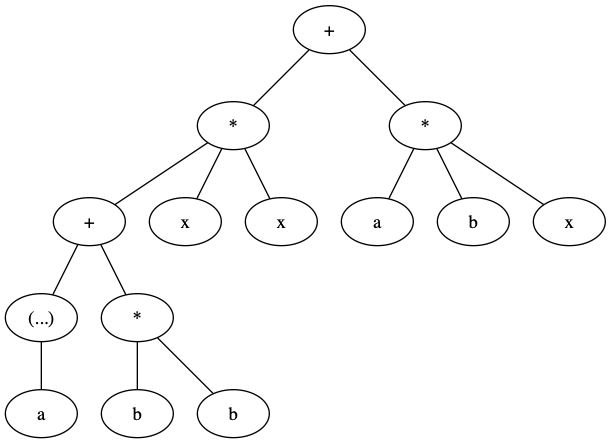
\includegraphics[width=11cm]{GRAPHICS/FORMULA_BUILDER/test_formula}
$$
\caption{\label{fig:ast:formula:example}The abstract synatx tree of the formula}
\end{figure}

\bigskip

The next example evaluates the formula over the field $\bbF_5,$ 
using the assignment $a=2,b=3,x=4$:
{\tt
\input GRAPHICS/THE_MAKEFILE/EXTRACTS/formula_evaluate.tex
}

\bigskip


\section{Basic Number Theory}
\label{sec:basic:number:theory}


\input C03/sec_1.tex


\bigskip




\clearpage



\section{Finite Fields}
\label{sec:finite:fields}


\input C03/sec_2.tex


\bigskip




\clearpage







\section{Extension Fields}
\label{sec:extension:fields}


\input C03/sec_3.tex


\bigskip




\clearpage


\section{Linear Algebra Over Finite Fields}
\label{sec:linear:algebra}


\input C03/sec_4.tex



\bigskip
\clearpage


\section{Advanced Topics in Finite Fields}
\label{sec:finite:field:advanced}


\input C03/sec_5.tex



\bigskip
\clearpage


\section{Basic Ring Theory}
\label{sec:ring:theory:basic}


\input C03/sec_6.tex



\bigskip
\clearpage


Table~\ref{tab:basic:number:theory} shows Orbiter commands for basic number theory, 
including integer factor rings and 
the Euclidean algorithm.
\begin{table}
\begin{center}
\begin{tabular}{|p{4cm}|p{3cm}|p{7cm}|}
\hline
Command & Arguments & Purpose \\
\hline
\hline
\verb'-power_mod' & $a$ $n$ $p$ & Computes $a^n$ mod $p$. \\
\hline
		\verb'-primitive_root' & $p$ & Computes a primitive root modulo $p$. \\
		\hline
		\verb'-discrete_log' & $b$ $a$ $p$ & Computes $n$ such that $a^n \equiv b \mod p$. \\
		\hline
		\verb'-extended_gcd' & $a$ $b$ & Computes integers $g,$ $u,$ and $v$ such that $g = \gcd(a,b) = ua + vb.$ \\
		\hline
		\verb'-square_root_mod' & $a$ $p$ & Computes a square root of $a$ modulo $p$, i.e. an integer $b$ such that $b^2 \equiv a$ mod $p$. \\
		\hline
		\verb'-square_root' & $a$ & Computes $\lfloor\sqrt{a}\rfloor$ of an integer $a$. \\
		\hline
		\verb'-inverse_mod' & $a$ $p$ & Computes the modular inverse of $a$ modulo $p$, i.e. an integer $b$ with $ab \equiv 1$ mod $p$. \\
		\hline
		\verb'-draw_mod_n' & descr & Draws the integers modulo $n$ on a circle. \\
		\hline
		\verb'-order_of_q_mod_n' & $q$ $n_{\min}$ $n_{\max}$ & Computes the order ${\rm ord}(q,n)$ 
		of $q$ modulo $n$ for all $n$ with $n_{\min} \le n \le n_{\max}$ 
		for which $\gcd(n,q) = 1$. Also computes $\varphi(n)$ and $\varphi(n)/{\rm ord}(q,n)$. \\
		\hline
		\verb'-Chinese_remainders' & R M & Solves a system of congruences with remainders R and moduli M. R and M must be vectors whose labels are given. \\
		\hline
\end{tabular}
\end{center}
\caption{\label{tab:basic:number:theory}Basic Number Theory Commands}
\end{table}


To compute primitive roots, the \verb'-primitive_root' command can be used.
The algorithm is randomized. 
For instance,  
{\tt
\input GRAPHICS/THE_MAKEFILE/EXTRACTS/PR29.tex
}
computes a primitive root modulo $29$. The answer in this case is $2.$
For a large example, consider
{\tt
\input GRAPHICS/THE_MAKEFILE/EXTRACTS/PR_915839.tex
}
which computes a primitive root modulo $915839$. The answer is $43085$.
The command 
{\tt
\input GRAPHICS/THE_MAKEFILE/EXTRACTS/PR_915839_check.tex
}
computes 
$$
43085^{49842} \mod 915839
$$
which is $487320$.

\bigskip

The command \verb'-discrete_log' can be used to compute the discrete logarithm of $a$ modulo $p$ with respect to $b$. 
This means, a number $k$ is computed such that 
$$
b^k \equiv a \mod p.
$$
For instance, the discrete log of $487320$ with respect to the base $43085$ modulo $915839$ is $49842,$ 
based on the previous example. 
We can compute the discrete logarithm 
using the command 
{\tt
\input GRAPHICS/THE_MAKEFILE/EXTRACTS/DL_915839.tex
}
This command can be quite expensive.

\bigskip

Computing inverses modulo  a prime $p$ is possible using the \verb'-inverse_mod' command. 
The command
{\tt
\input GRAPHICS/THE_MAKEFILE/EXTRACTS/IM.tex
}
computes the inverse of $1865025205$ modulo $2147483647$ which is $579785381.$

\bigskip


A different way of computing the inverse is using the 1-trick. 
This approach computes the gcd of two numbers $a$ and $b$, say, 
and writes 
$$
\gcd(a,b)  = ua+vb
$$
for some $u,v \in \bbZ$. 
The \verb'-extended_gcd' command can be used. For instance, the following command 
computes the gcd of  $a=2147483647$  and $b=1865025205$.
{\tt
\input GRAPHICS/THE_MAKEFILE/EXTRACTS/IM_gcd.tex
}
The output is
$$
1 = -503526232 * 2147483647 + 579785381 * 1865025205,
$$
from which we see that $\gcd(a,b) = 1$ and $u= -503526232$ and $v = 579785381.$
which is the gcd written as a lattice combination of the input arguments. 
The inverse of $1865025205$  mod $2147483647$ is $v=579785381.$

\bigskip

In order to compute the modular power
$$
a^e \mod n,
$$
the \verb'-power_mod' command can be used. For instance, 
{\tt
\input GRAPHICS/THE_MAKEFILE/EXTRACTS/PM3a.tex
}
computes 
$16807$ raised to the power $1073741823$ modulo $2147483647,$ which is $2147483646.$

\bigskip

The modular square root of $a$ modulo $p$ is any $x$ in 
$$
x^2 \equiv a \mod p.
$$
Thecommand \verb'-square_root_mod' can be used to compute modular square roots using 
the algorithm of Tonelli and Shanks (cf.~\cite{Cohen93}).
For instance, 
{\tt
\input GRAPHICS/THE_MAKEFILE/EXTRACTS/sqrt_mod.tex
}
finds that the square root of $33$ mod $41$ is $19,$
i.e.
$$
19^2 \equiv 33 \mod 41.
$$

\bigskip


The command \verb'order_of_q_mod_n'
computes  ${\rm ord}(q,n)$, the order of $q$ modulo $n$, 
for all $n$ with $n_{\min} \le n \le n_{\max}$ and $\gcd(n,q) = 1$. 
It also computes Euler's totient function $\varphi(n)$ 
and the cofactor $\varphi(n)/{\rm ord}(q,n).$
For instance, 
{\tt
\input GRAPHICS/THE_MAKEFILE/EXTRACTS/order_of_2_mod_n.tex
}
produces the output shown in Table~\ref{tab:order}.
\begin{table}
$$
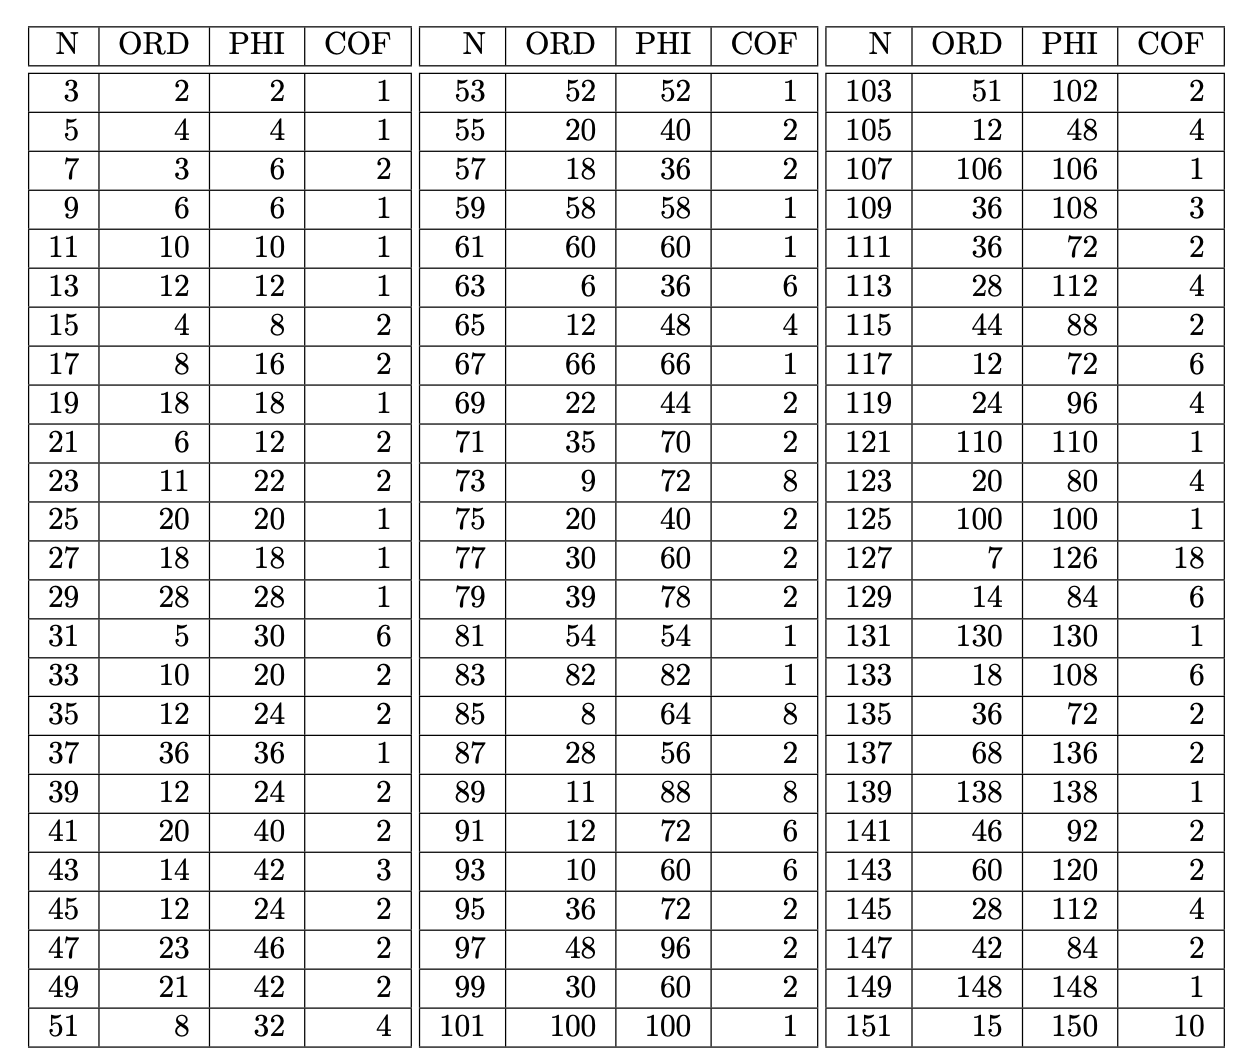
\includegraphics[width=11cm]{GRAPHICS/NUMBER_THEORY/order_of_2}
$$
\caption{\label{tab:order}The order of $2$ modulo $n$}
\end{table}

\bigskip


The command 
{\tt
\input GRAPHICS/THE_MAKEFILE/EXTRACTS/Eulerfunction_150.tex
}
computes Euler's totient function for all integers $n$ with $1 \le n \le 150.$
The result is shown in Table~\ref{tab:eulerfunction}.
\begin{table}
$$
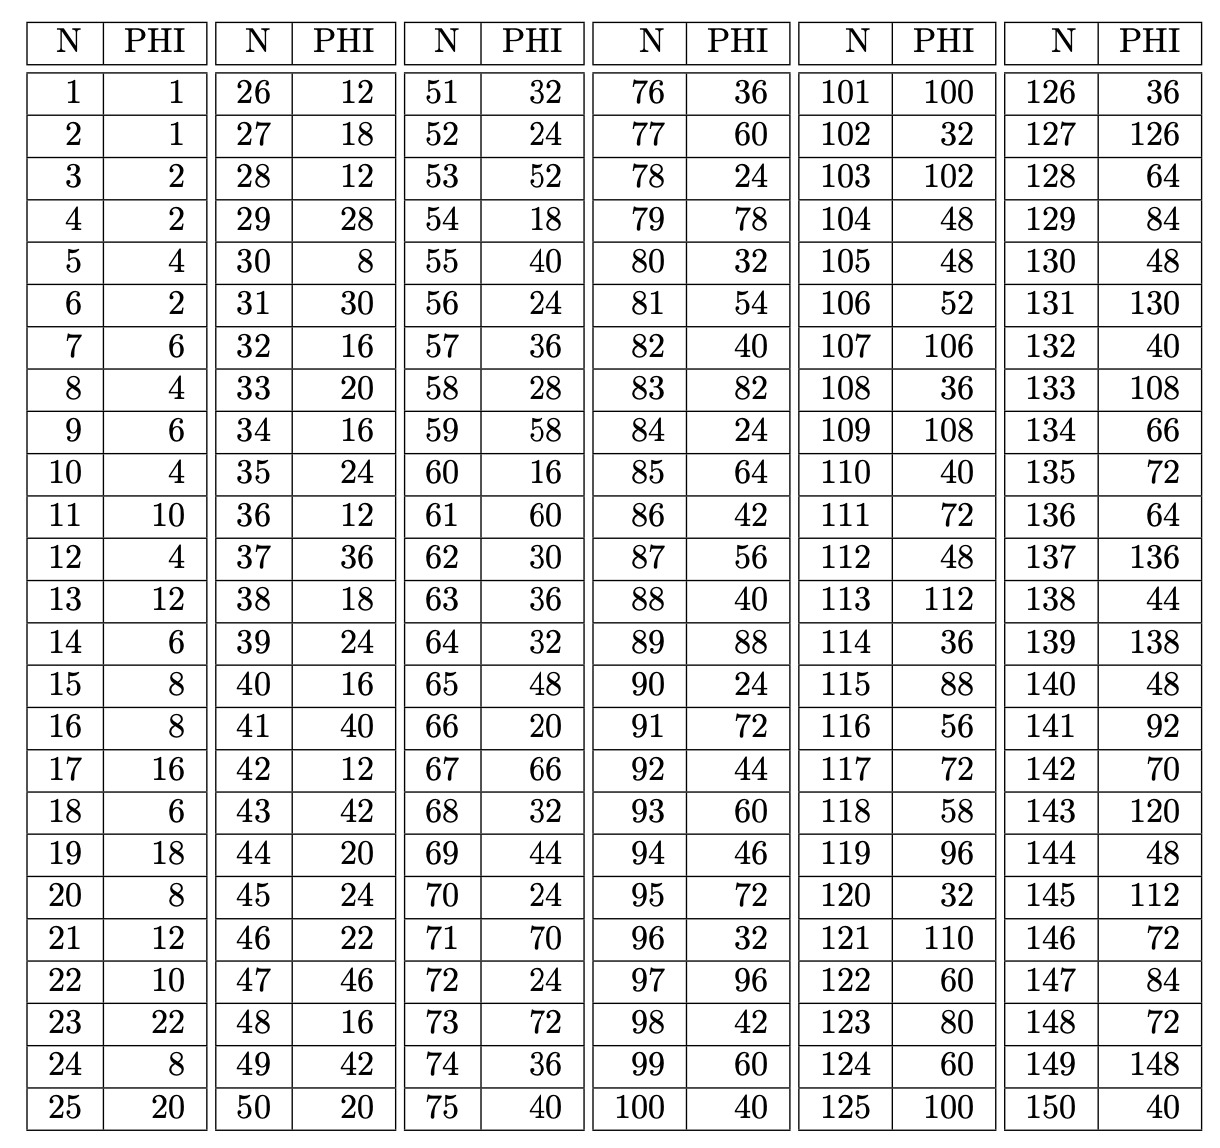
\includegraphics[width=11cm]{GRAPHICS/NUMBER_THEORY/eulerfunction_150}
$$
\caption{\label{tab:eulerfunction}The values of the Eulerfunction}
\end{table}

\bigskip

A power map sends $a$ to $a^k$ for some fixed $k$. 
Orbiter can compute power maps modulo $p$. 
For instance, the following command computes the function $a \mapsto a^k \mod 11$:
{\tt
\input GRAPHICS/THE_MAKEFILE/EXTRACTS/power_function_2_mod_11.tex
}
The result is shown in Table~\ref{tab:eulerfunction}.
\begin{table}
$$
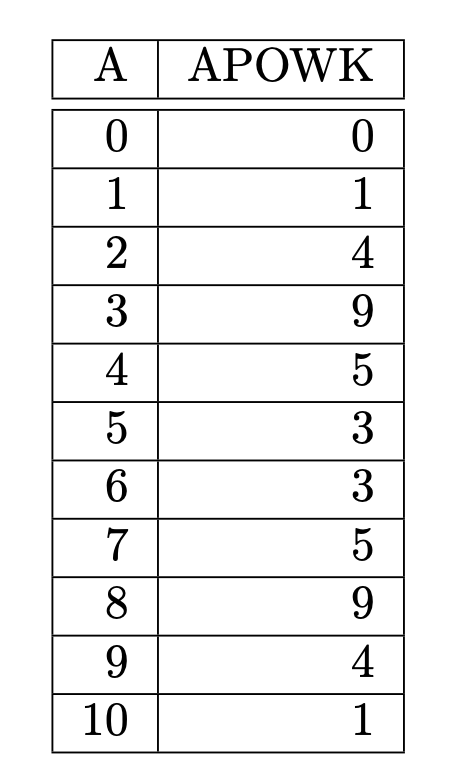
\includegraphics[width=3cm]{GRAPHICS/NUMBER_THEORY/a_pow_2_mod_11}
$$
\caption{\label{tab:power:2:11}The function $a \mapsto a^2$ mod $11$}
\end{table}

\bigskip

It is sometimes helpful to draw the elements modulo $n$ on a circle, 
using the vertices of an $n$-gon to represent the field elements. For instance, for 
the command 
{\tt
\input GRAPHICS/THE_MAKEFILE/EXTRACTS/draw_mod_13.tex
}
uses a $13$-gon to represent the elements modulo $13$. 
It also computes the powers of $2$ mod $13$ and connects 
consecutive powers in the diagram (see Figure~\ref{ref:power:13}).
\begin{figure}
$$
\begin{array}{c}
\input GRAPHICS/MOD13/mod_13_powers_of_2_draw.tex\\
\end{array}
$$
\caption{\label{ref:power:13}Cycle of powers of $2$ modulo $13$}
\end{figure}

\bigskip

The next command illustrates how to solve a system of congruences with coprime moduli 
using the Chinese remainder theorem.
Suppose we want to find the integer $x$ such that 
\begin{eqnarray*}
x & \equiv 2 \; \mbox{mod} \; 5\\
x & \equiv 2 \; \mbox{mod} \; 6\\
x & \equiv 5 \; \mbox{mod} \; 7\\
\end{eqnarray*}
The following command creates one vector for the remainders and one for the moduli and then 
invokes the \verb'-Chinese_remainders' command.
{\tt
\input GRAPHICS/THE_MAKEFILE/EXTRACTS/Chinese_remainders_A.tex
}
The answer is $x \equiv 152$ modulo 210.

\bigskip

The next example shows that the Chinese remainder algorithm is safe for large numbers.
We pick two 10 digit prime numbers as moduli and solve 
\begin{eqnarray*}
x & \equiv 2 \; \mbox{mod} \; 2147483647\\
x & \equiv 3 \; \mbox{mod} \; 5915587277\\
\end{eqnarray*}
using the command
{\tt
\input GRAPHICS/THE_MAKEFILE/EXTRACTS/Chinese_remainders_C2.tex
}
The answer is 
$$
x \equiv 5684294357108828365 \mod 12703626939758759219.
$$
A quick check with Maple shows that 
\begin{eqnarray*}
5684294357108828365 \mod 2147483647 & \equiv 2 \\
5684294357108828365 \mod 5915587277 & \equiv 3 \\
\end{eqnarray*}
as required.



Let $\bbF_q$ denote the finite field with $q$ elements. 
Up to isomorphism, there is only one field of order $q$. 
See Section~\ref{sec:limitations} for a list of limitations of Orbiter.
A finite field $\bbF_q$ can be created using the 
\verb'-finite_field'
command.
Table~\ref{tab:finitefield:create} lists Orbiter commands for creating a finite field.
\begin{table}
	\begin{center}
	\begin{tabular}{|p{4cm}|p{3cm}|p{7cm}|}
		\hline
		Command & Arguments & Purpose \\
		\hline
		\hline
		\verb'-q' & $q$ &  Specify the order of the field. Here, $q=p^k$  for some prime $p$ and some positive integer $k$. \\
		\hline
		\verb'-override_' \verb'polynomial' & $n$  &  Specify the polynomial used to create the finite field. 
		The polynomial is given as integer, using the base $p$ representation. See Section~\ref{sec:extension:fields}. \\
		\hline
		\verb'-without_tables' &  &  Create the field without precomputing the tables.  \\
		\hline
		\end{tabular}
	\end{center}
	\caption{\label{tab:finitefield:create}Options for Creating Finite Fields}
	\end{table}
For instance,  
{\tt
\input GRAPHICS/THE_MAKEFILE/EXTRACTS/F_2.tex
}
creates the finite field $\bbF_2$ and produces a report for it.

\bigskip


Table~\ref{tab:finitefield:activities} lists basic Orbiter activities for finite fields. 
More activities will follow in Section~\ref{sec:extension:fields}.  
\begin{table}
	\begin{center}
	\begin{tabular}{|p{4cm}|p{3cm}|p{7cm}|}
		\hline
		Command & Arguments & Purpose \\
		\hline
		\hline
		\verb'-cheat_sheet_GF' &  &  Produce a cheat sheet in latex which shows information about the field, including addition and multiplication tables.  \\
		\hline
		\verb'-product_of' & $v$ &  Compute the product of all field elements in the vector $v$.  \\
		\hline
		\verb'-sum_of' & $v$ &  Compute the sum of all field elements in the vector $v$.  \\
		\hline
		\verb'-negate' & $v$ &  Negate each field element in the vector $v$.  \\
		\hline
		\verb'-inverse' & $v$ &  Compute the multiplicative inverse of each field element in the vector $v$.  \\
		\hline
		\verb'-power_map' & $k$ $v$ &  Compute the $k$-th power of each field element in the vector $v$.  \\
		\hline
		\end{tabular}
	\end{center}
	\caption{\label{tab:finitefield:activities}Finite Field Activities}
	\end{table}
The command  
{\tt
\input GRAPHICS/THE_MAKEFILE/EXTRACTS/F_7.tex
}
creates a cheat sheet for $\bbF_7$ as shown below. 
The element $\alpha$ is a primitive element. 

\bigskip



\begin{mdframed}[style=MyFrame]
\input GRAPHICS/LATEX/report_finite_field_7.tex
\end{mdframed}



\bigskip



Suppose we want to check Wilson's theorem that the product of all nonzero field elements of negative one.
The following command so so, assuming that $p = 11.$ We first create a vector of all 
nonzero field elements, which we take as the integers from $1$ to $10$. After that, 
we use the \verb'product_of' finite field activity to compute the product of these elements. 
The answer is $10$ which is congruent to $-1$ mod $11:$
{\tt
\input GRAPHICS/THE_MAKEFILE/EXTRACTS/F_11_product_of_all_nonzero_elements.tex
}


\bigskip


Suppose we want to create the Vandermonde matrix whose entries are $x_{i}^j$. 
Here $x_0,\ldots,x_{q-1}$ are the elements of the field $\bbF_q$ 
and $j$ ranges from $0$ to $q-1$. The following command does so for $q=7$. 
The command also computes the inverse of the Vandermonde matrix.
{\tt
\input GRAPHICS/THE_MAKEFILE/EXTRACTS/F_7_vandermonde.tex
}
The output is shown below. The first matrix is $V = (x_{i}^j).$ The second matrix is $V^{-1}$:
\begin{mdframed}[style=MyFrame]
\input GRAPHICS/LATEX/report_finite_field_7_vandermonde.tex
\end{mdframed}


\bigskip



There is a second ordering of the elements which is used occasionally. 
In this labeling, every non-zero element is written as a power of a fixed primitive element.
So, if $\alpha$ is a primitive element, we arrange the elements of $\bbF_p$ as 
$$
0,1,\alpha,\alpha^2,\ldots,\alpha^{q-2}.
$$
The cheat sheet contains this list of field elements at the very end.
In Figure~\ref{fig:fieldtables7rearranged}, 
\begin{figure}
$$
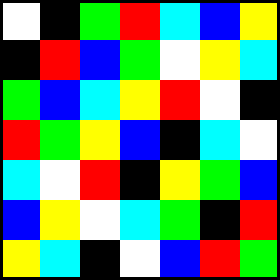
\includegraphics[width=5cm]{GRAPHICS/GF/GF_q7_addition_table_reordered_draw}
\qquad
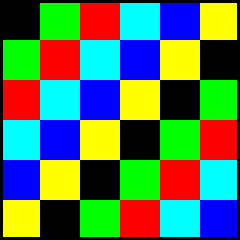
\includegraphics[width=5cm]{GRAPHICS/GF/GF_q7_multiplication_table_reordered_draw}
$$
\caption{\label{fig:fieldtables7rearranged}Addition and multiplication table 
of $\bbF_7$ using a primitive element}
\end{figure}
the addition and multiplication tables of $\bbF_7$ are shown 
with respect to the cyclic ordering of elements as
$$
0,3^0,3^1,3^2,\ldots,3^6 = 0,1,3,2,6,4,5,1.
$$
In the second ordering, the addition table of 
the prime field no longer exhibits cyclic structure.






\bigskip


For small field orders, the Orbiter employs 
precomputed tables for the arithmetic operations such as addition and multiplication and computing inverses.
Precomputing these tables can be time-consuming. 
The option \verb'-without_tables' can be given to avoid precomputing tables. 
Here is an example. 
We create the field $\bbF_{101}$ without precomputed tables:
{\tt
\input GRAPHICS/THE_MAKEFILE/EXTRACTS/F_101_wo.tex
}



\bigskip






Let $F$ be a field. An extension field of $F$ is any field $E$ which contains $F.$
Because $E$ is a vector space over $F$, the dimension of $E/F$ is wel-defined. 
It may be finite or infinite.
An example of a field extension is a field of the form $E = F(\alpha)$, 
where $\alpha$ is any element over $F.$
Here, $F(\alpha)$ is the smallest field which contains $F$ and $\alpha.$
If $\gamma \in E$ satisfies a polynomial equation with coefficients in $F,$ 
then $\gamma$ is called algebraic over $F$.
The minimum polynomial of an element $\gamma$ in $E$ over $F$ is the monic, lowest degree 
polynomial in $F[X]$ which has $\gamma$ as a root. 
A field extension $E/F$ is algebraic if every element in $E$ is algebraic over $F$. 
In particular, $F(\alpha)$ is algebraic over $F$ if $\alpha$ is. 
The degree of $E/F$ equals the degree of the minimum polynomial of $\alpha$ over $F$.

\bigskip


In this section, we will consider algebraic extension of finite fields. 
If $F = \bbF_q$ is a field of order $q$, then any algebraic extension $E$ 
of $F$ has order $q^e$ where $e$ is the degree of $E$ over $F$.
If $E = F(\alpha)$ is algebraic, the degree of $E$ over $F$ 
is the degree of the minimum polynomial of $E$ over $F$.
If $F = \bbF_q$ and $E = F(\alpha)$ is algebraic of degree $e$, then $|F| = q^e.$
Every finite field $E$ is of this form, where $F = \bbF_p$ and $p$ is the characteristic of $E$.

\bigskip

Any such $E$ can be constructed as a polynomial factorring of the ring $\bbF_p[X].$
For a polynomial $m(X)$ we consider the ideal 
$$
\bI(m) = m(X)\bbF_p[X] = \{m(X)k(X) \mid k(X) \in \bbF_p[X] \} 
$$
of all polynomial multiples of $m(X).$
Under the assumption that $m(X)$ has degree $e > 1$ and is irreducible, 
the residue class ring 
$$
\bbF_p[X]/ \bI(m)
$$
is a field with $q = p^e$ elements.
Each residue class has a canonical representative. The canonical representative is the unique element 
in the residue class which has degree less than $e$ and leading coefficient one. 
By means of identification, we can take these polynomials to be the set of standard representatives 
of the residue classes. 
So, for instance, for $q = 4 = 2^2,$ we can pick the irreducible polynmial 
$m(X) = X^2+X+1$ over $\bbF_2$ and have four standard representatives modulo $\bI(m),$ namely
$$
\begin{array}{c}
0, \\
1, \\
X, \\
X + 1.\\
\end{array}
$$
Together, these make up a complete set of representatives of the residue classes modulo  $\bI(m),$ 
and hence can be identified with the elements of $\bbF_4$:
$$
\bbF_4 = \{0, \; 1, \; X, \; X+1 \}.
$$
The addition of polynomials is as in $\bbF_2[X],$ so 
$$
\begin{array}{c|cccc}
 & 0 & 1 & X & X + 1 \\
\hline
0 & 0 & 1 & X & X + 1\\
1 & 1 & 0 & X+1 & X \\
X & X & X + 1 & 0 & 1 \\
X + 1 & X + 1 & X & 1 & 0 \\
\end{array}
$$
To compute the multiplication table for the field $\bbF_4$.
We can use polynomial arithmetic modulo $m(X):$
It is clear how multiplication by $0$ or $1$ works, so we need to focus on the 
polynomials $X$ and $X+1$:
$$
\begin{array}{lllll}
X &\cdot\; X &= X^2 &\equiv X + 1 &\mod X^2 + X + 1, \\
X &\cdot\; (X+1) &= X^2+X &\equiv 1 &\mod X^2 + X + 1, \\
(X+1) &\cdot\; X &= X^2+X &\equiv 1 &\mod X^2 + X + 1, \\
(X+1) &\cdot\; (X+1) &= X^2+1 &\equiv X &\mod X^2 + X + 1, \\
\end{array}
$$
so the multiplication table of $\bbF_4$ turns out to be
$$
\begin{array}{c|cccc}
 & 0 & 1 & X & X + 1 \\
\hline
0     & 0 & 0   & 0 & 0\\
1     & 0 & 1   & X & X+1 \\
X     & 0 & X   & X+1 & 1 \\
X + 1 & 0 & X+1 & 1 & X \\
\end{array}
$$
Figure~\ref{fig:fieldtables4} shows a graphical representation of the 
addition and multiplication tables of $\bbF_4$ using colors to represent the different elements: 
White is zero, black is one, red is $X$ and green is $X+1.$
\begin{figure}
$$
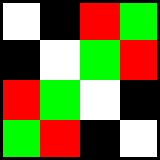
\includegraphics[width=3cm]{GRAPHICS/GF/GF_q4_addition_table_draw} 
\quad 
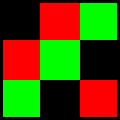
\includegraphics[width=3cm]{GRAPHICS/GF/GF_q4_multiplication_table_draw}
$$
\caption{\label{fig:fieldtables4}Addition and multiplication tables of $\bbF_4$}
\end{figure}
In the multiplication table, the row and column associated with the zero elements are removed.

\bigskip

Table~\ref{tab:finitefield:activities:more} lists Orbiter activities for finite fields. 
This extends Table~\ref{tab:finitefield:activities} in Section~\ref{sec:extension:fields}.  
\begin{table}
	\begin{center}
	\begin{tabular}{|p{4cm}|p{3cm}|p{7cm}|}
		\hline
		Command & Arguments & Purpose \\
		\hline
		\hline
		\verb'-trace' &   &  Computes the partition of the field elements according to the value of their absolute trace.   \\
		\hline
		\verb'-norm' &   &  Computes the partition of the field elements according to the value of their absolute norm.  \\
		\hline
		\verb'-normal_basis' & $d$  &  Computes a normal basis for $\bbF_{q^d}.$  \\
		\hline
		\end{tabular}
	\end{center}
	\caption{\label{tab:finitefield:activities:more}More Finite Field Activities}
	\end{table}


\bigskip


The isomorphism type of the resulting field only depends on the order $q$ of the field, 
and not on the choice of the polynomial. 
However, for practical computations, the choice of the polynomial matters. 
For instance, results can only be shared between different computer algebra systems if the same polynomials are used.
Orbiter has a large collection of polynomials built in. 
Besides these, a polynomial can be specified.
The polynomials that Orbiter offers are in fact primitive, which means that the 
root $\alpha$ is a primitive element for the field $\bbF_q.$ 
This just means that it is a generator of the multiplicative group. 
So, any non-zero element in $\bbF_q$ 
is a suitable power of $\alpha.$


\bigskip

If $\bbF_q$ is an extension of the prime field $\bbF_p$, we use a different labeling.
This time, we exploit the fact that $\bbF_q$ is a vector space over $\bbF_p.$
Let $\alpha$ be a root of the irreducible polynomial $m(X)\in \bbF_p[X]$ used to create the field. 
Suppose that $q=p^e,$ i.e., the degree of $m(X)$  is $e$.
An $\bbF_p$-basis for the vector space $\bbF_q$ over $\bbF_p$ is given by the powers 
$\alpha^i,$ for $0 \le i < e.$ 
Therefore, any element $\gamma$ of $\bbF_q$ has a unique expression of the form 
$$
\gamma = \sum_{h=0}^{e-1} a_i \alpha^i, \quad  0 \le a_i < p  \;\mbox{for all} \; i.
$$
The associated integer rank of $\gamma$ is obtained by replacing $\alpha$ by $p$ in this expression 
and evaluating the expression over the integers. 
So, the rank of $\gamma$ is 
$$
\sum_{h=0}^{e-1} a_i p^i.
$$
As $\gamma$ ranges over all field element in $\bbF_q,$ 
the rank values take on every value in the interval $[0,q-1].$ 
The ordering of elements of $\bbF_q$ according to these ranks is called the lexicographical ordering. 
The numerical rank of zero is $0$ and the numerical rank of one is $1$.
The numerical rank of $\alpha,$ the primitive element, is $p.$
The numerical ranks of the elements of the prime subfield are exactly the elements of $[0,p-1].$
%This makes for an interesting effect when displaying the addition and multiplication tables of the extension field. 

\bigskip

The primitive polynomials used by Orbiter to create small finite fields 
are listed in Table~\ref{tab:primitive:polynomials}. 
The relation is given using the Greek letter that 
is used in orbiter cheat sheets for that particular field.
\begin{table}
\begin{center}
\begin{tabular}{|r|r|r|l|}
\hline
$q$  & Polynomial & Numerical & Relation \\
\hline
\hline
4 & $X^2+X+1$ & 7 & $\omega^2 = \omega+1$ \\
8 & $X^3 + X^2 + 1$ & 13 & $\gamma^3 = \gamma^2+1$ \\
9 & $X^2 + X + 2$ & 14 & \\
16 & $X^4 + X^3 + 1$ & 25 &$\delta^4=\delta^3+1$ \\
25 & $X^{2} + X + 2$ & 22 & \\
27 & $X^3 + 2X + 1$ & 34 & \\
32 & $X^5 + X^2 + 1$ & 37 & $\eta^5=\eta^2+1$ \\
49 & $X^{2} + X + 3$ & 59 & \\
64 & $X^6 + X^5 + 1$ & 97 & \\
81 & $X^4 + X^3 + 2$ & 110 & \\
121 & $X^{2} + 4X + 2$ & 167 & \\
125 & $X^{3} + X^{2} + X + 2$ & 86 & \\
128 & $X^7 + X^6 + 1$ & 193 & $\zeta^7=\zeta^6+1$ \\
169 & $X^{2} + X + 2$ & 184 & \\
243 & $X^5 + 2X + 1$ & 250 & \\
256 & $X^8 + X^4 + X^3 + X^2 + 1$ & 285 & \\
289 & $X^{2} + X + 3$ & 309 & \\
343 & $X^{3} + 3X + 2$ & 366 & \\
361 & $X^{2} + X + 2$ & 382 & \\
512 & $ X^9 + X^4 + 1$ & 529 & \\
529 & $X^{2} + 2X + 5$ & 580 & \\
625 & $X^{4} + X^{3} + X + 2$ & 326 & \\
729 & $X^6 + X^5 + 2$ & 974 & \\
841 & $X^{2} + 5X + 2$ & 988 & \\
961 & $X^{2} + 2X + 3$ & 1026 & \\
1024 & $X^{10} + X^3 + 1$ & 1033 & \\
\hline
\end{tabular}
\end{center}
\caption{\label{tab:primitive:polynomials}Orbiter primitive polynomials for fields $\bbF_q$ with $q \le 1024$}
\end{table}




%The tables of the prime field appear in the upper left corner, as seen for instance in 
%Figure~\ref{fig:fieldtables49} for $\bbF_{49}$.
%\begin{figure}
%$$
%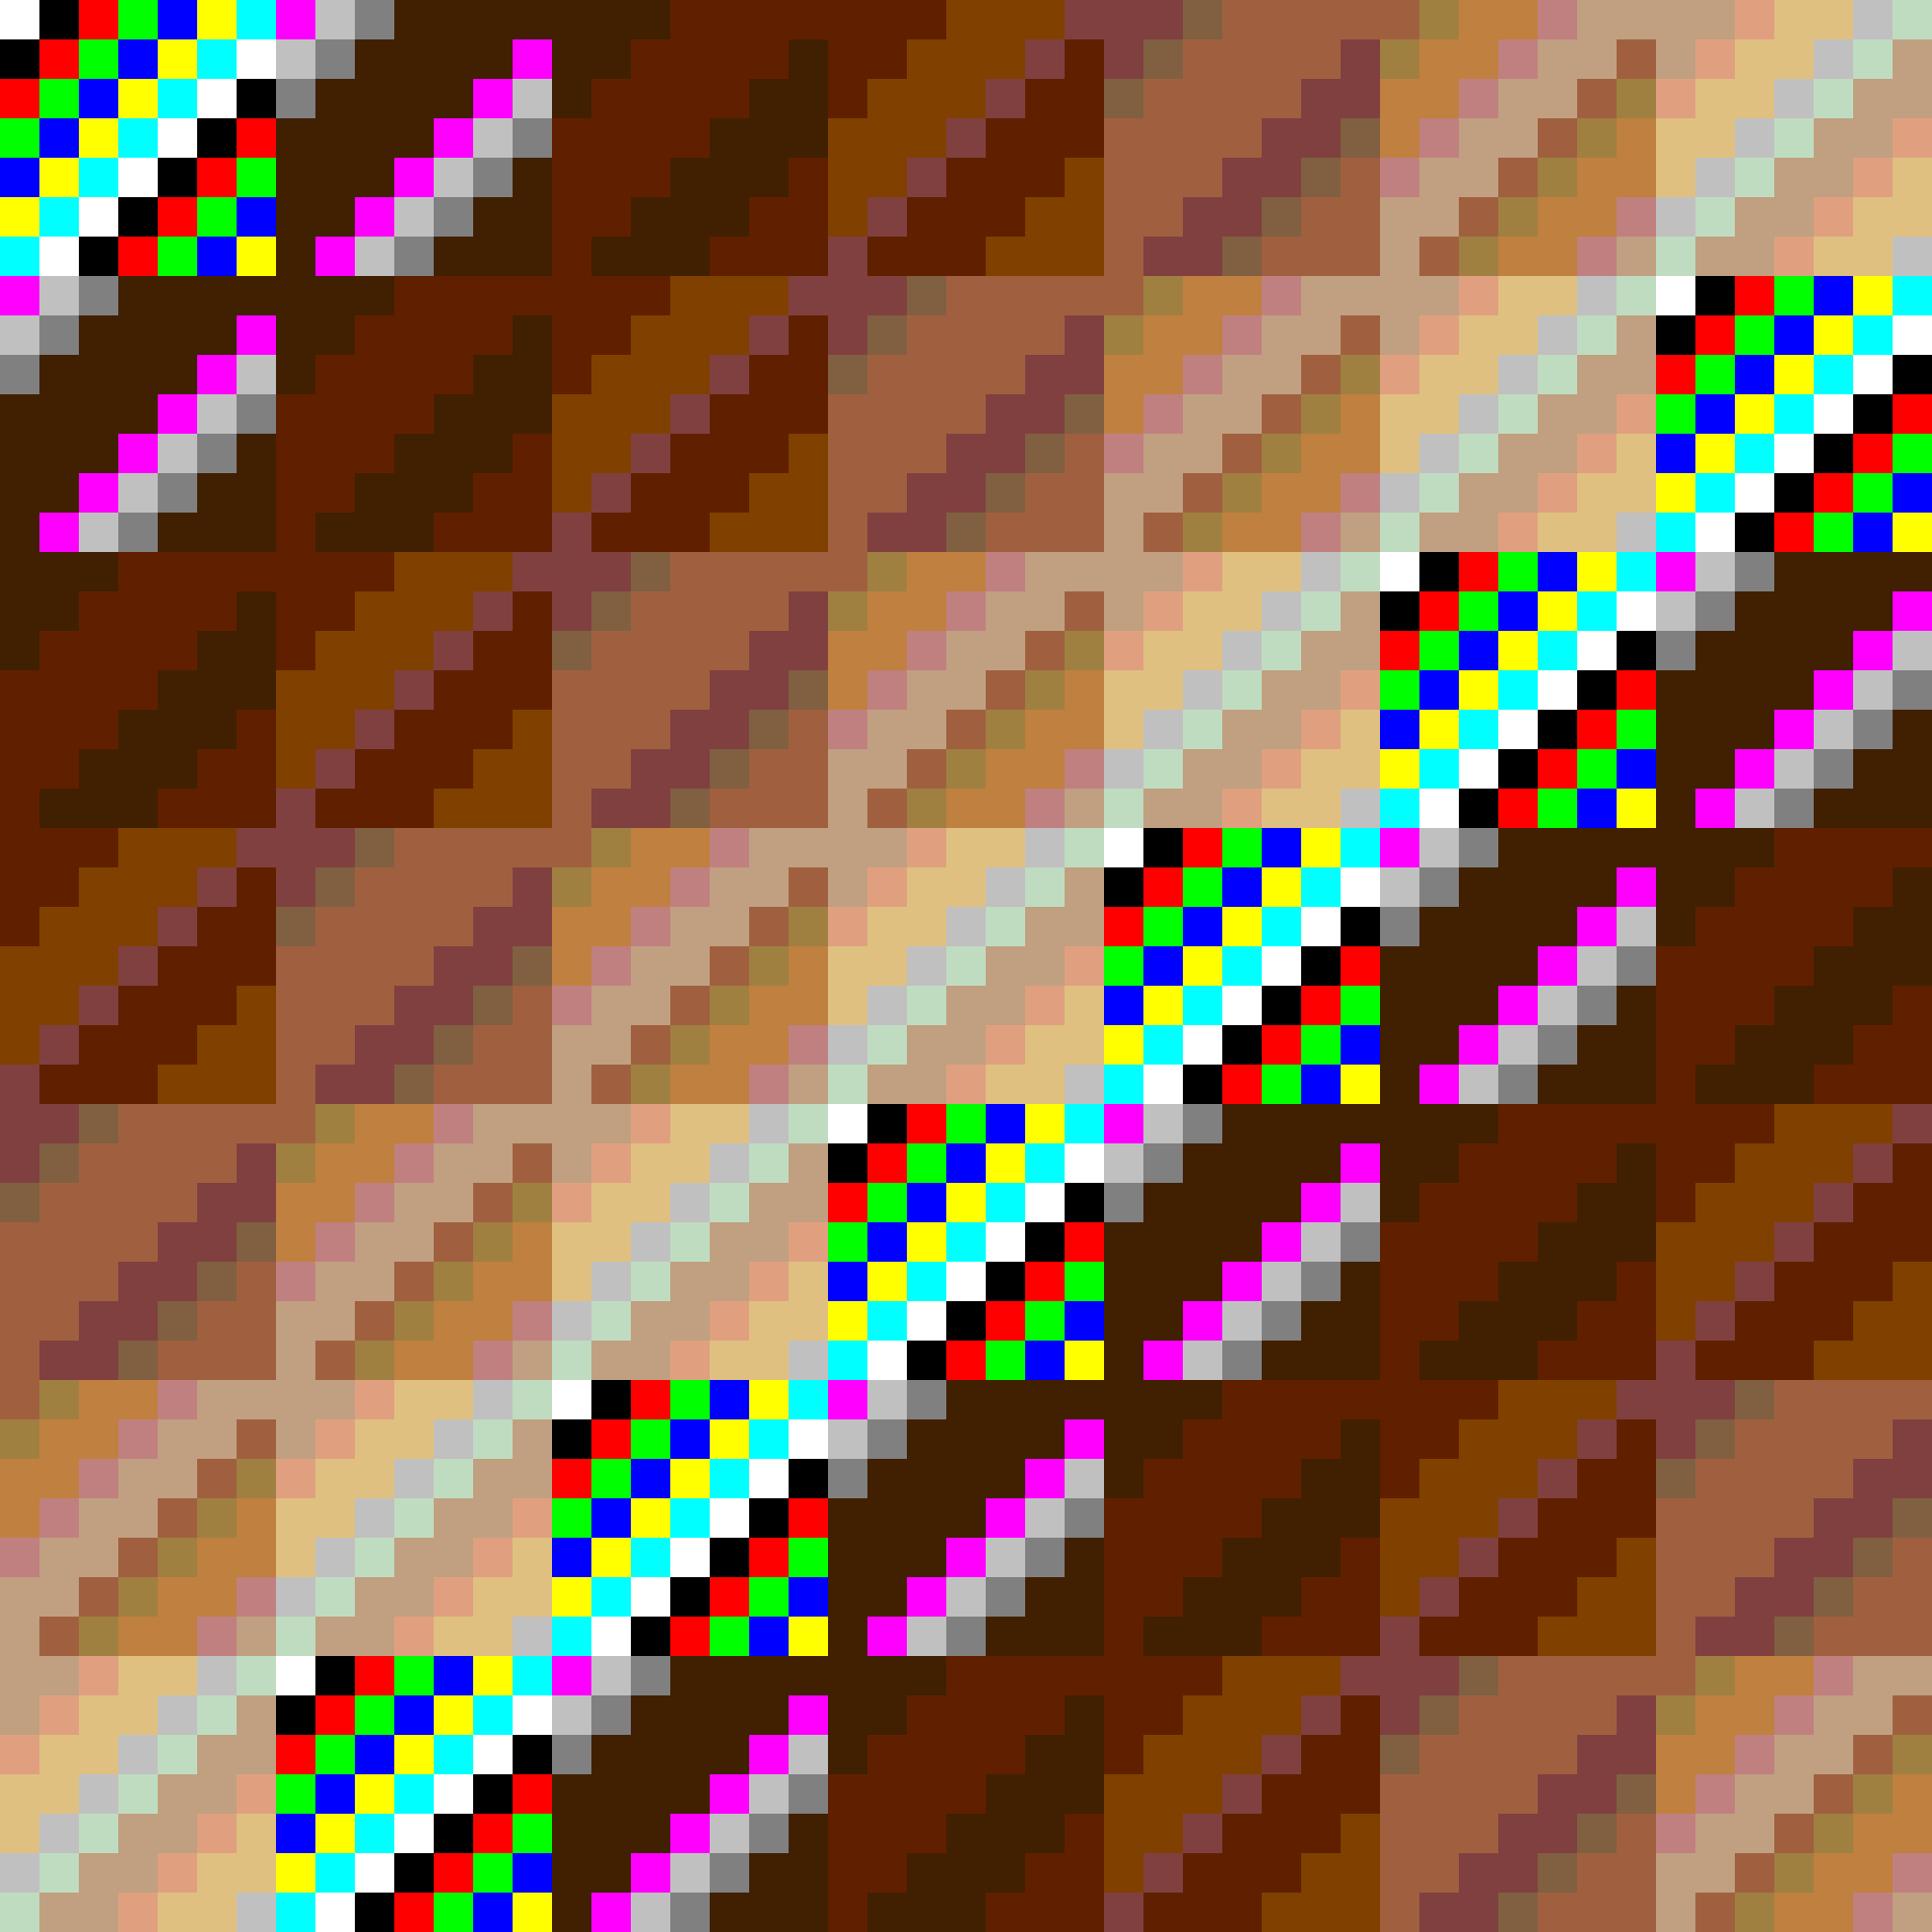
\includegraphics[width=7.5cm]{GRAPHICS/GF/GF_q49_addition_table_draw}
%\qquad
%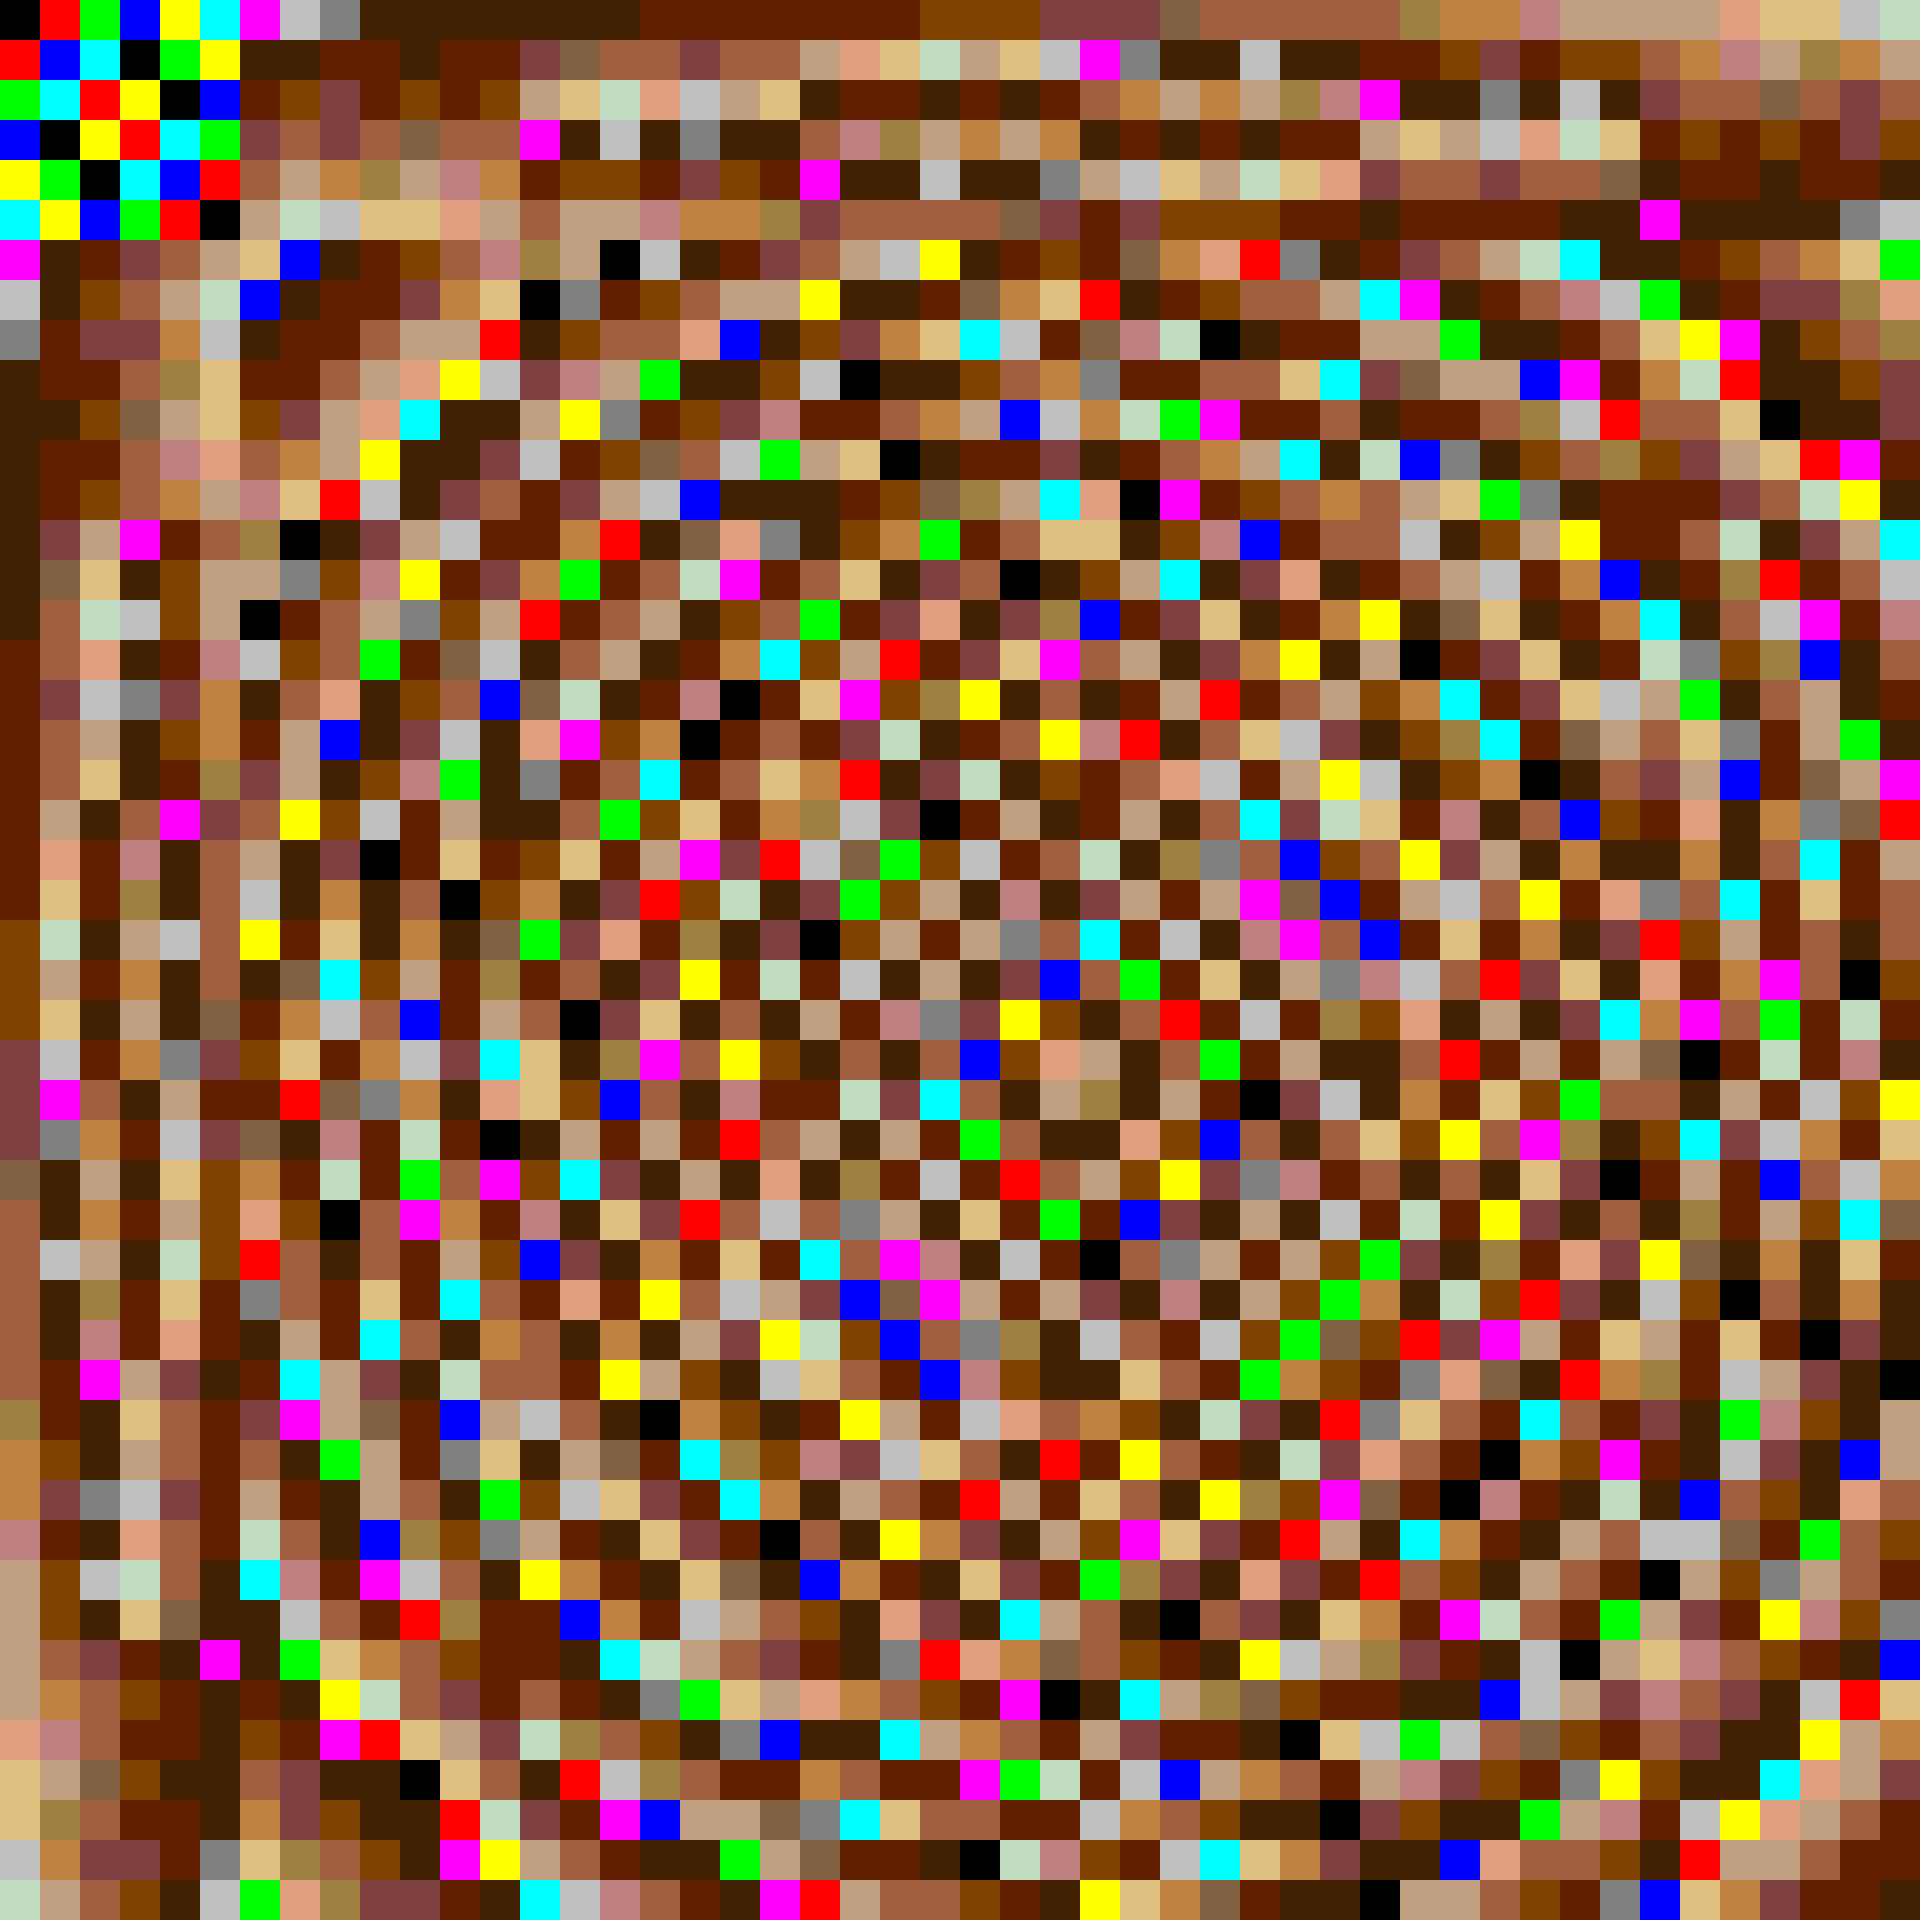
\includegraphics[width=7.5cm]{GRAPHICS/GF/GF_q49_multiplication_table_draw}
%$$
%\caption{\label{fig:fieldtables49}Addition and multiplication table of $\bbF_{49}$ using the lexicographic ordering of elements}
%\end{figure}
%The following Orbiter command was used to create the tables:
%\begin{verbatim}
%orbiter.out -cheat_sheet_GF 49
%\end{verbatim}

\bigskip

Let us look at a few examples. 
The command 
{\tt
\input GRAPHICS/THE_MAKEFILE/EXTRACTS/F_4.tex
}
creates a report for the field $\bbF_4.$
The command 
{\tt
\input GRAPHICS/THE_MAKEFILE/EXTRACTS/F_16.tex
}
creates a cheat sheet for $\bbF_{16}.$
This command produces Table~\ref{tab:GF16}.
\begin{table}
\begin{mdframed}[style=MyFrame]
$$
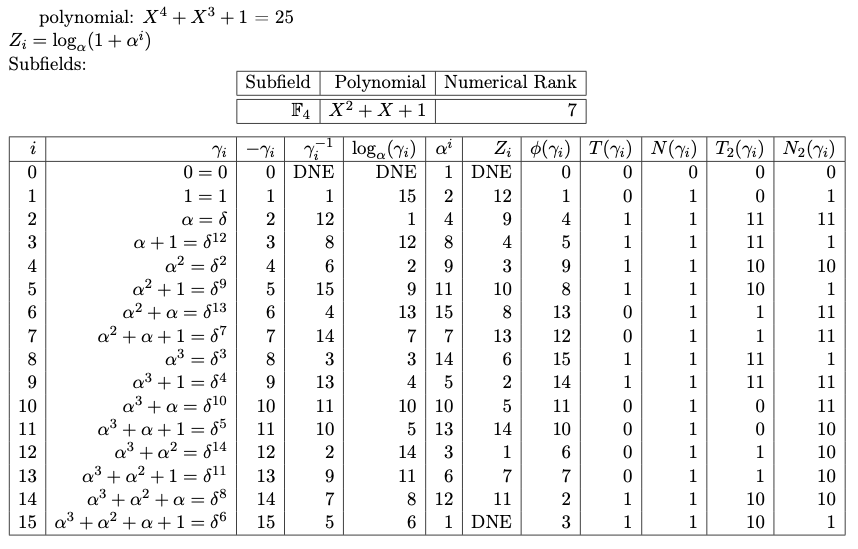
\includegraphics[width=14cm]{GRAPHICS/GF/cheat_sheet_GF16}
$$
\end{mdframed}
\caption{\label{tab:GF16}The field $\bbF_{16}$}
\end{table}




\bigskip


Unlike other computer algebra systems (GAP~\cite{GAP} and Magma~\cite{Magma}),
Orbiter does not use Conway polynomials to create field extensions. 
Instead, it  
provides the option to override the polynomial used to create the finite field.
For subfield relationships, the cheat sheet will indicate the irreducible polynomials 
of all subfields for a given field.  
For instance, Table~\ref{tab:GF64subfields} shows the subfields of $\bbF_{64}$ 
generated by the polynomial $X^{6} + X^{5} + 1$  whose numerical rank is 97.
\begin{table}
$$
\begin{array}{|r|r|r|}
\hline
\mbox{Subfield} & \mbox{Polynomial} & \mbox{Numerical rank} \\
\hline
\hline
\bbF_{4}  & X^{2} + X + 1& 7\\
\hline
\bbF_{8}  & X^{3} + X + 1& 11\\
\hline
\end{array}
$$
\caption{\label{tab:GF64subfields}The subfields of $\bbF_{64}$}
\end{table}


\bigskip

The lexicographic ordering has an interesting side-effect for the ordering of elements in extension fields. The elements of the prime subfield are always listed before any other elements in the extension field. 
For this reason, the addition and multiplication tables of the extension field contain the 
respective table of the prime field in the upper left corner.
For instance, in Figure~\ref{fig:fieldtables:9}, we find the tables for $\bbF_3$ 
in the upper left corners of the tables of $\bbF_9$, for instance.
\begin{figure}
$$
\begin{array}{ll}
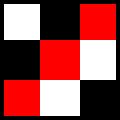
\includegraphics[width=2cm]{GRAPHICS/GF/GF_q3_addition_table_draw}
&
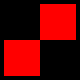
\includegraphics[width=1.5cm]{GRAPHICS/GF/GF_q3_multiplication_table_draw}
\\[10pt]
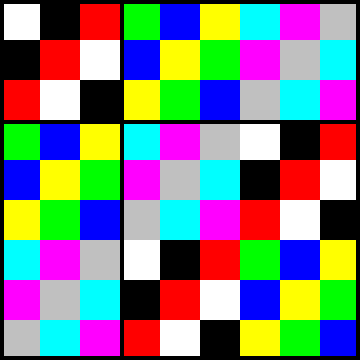
\includegraphics[width=6cm]{GRAPHICS/GF/GF_q9_addition_table_draw}
&
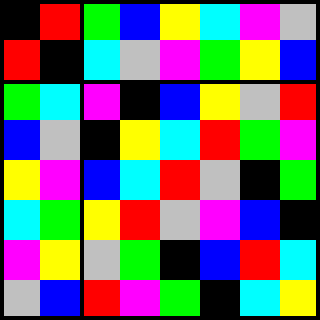
\includegraphics[width=6cm]{GRAPHICS/GF/GF_q9_multiplication_table_draw}
\\
\end{array}
$$
\caption{\label{fig:fieldtables:9}Addition and multiplication table 
of $\bbF_{3}$ and $\bbF_{9}$ using the lexicographic ordering of elements}
\end{figure}
Recall that omit the zero element in the multiplication tables.


\bigskip

Orbiter uses primitive polynomials for creating extension fields. Because of this, 
the element $\alpha$ is always primitive. 
Since the numerical rank of $\alpha$ is $p,$ this means that the rank $p$ 
always represents a primitive element in an extension field.
For the addition and multiplication tables of $\bbF_{9}$ 
arranged with respect to powers of a primitive element, see 
Figure~\ref{fig:fieldtables9rearranged}. 
\begin{figure}
$$
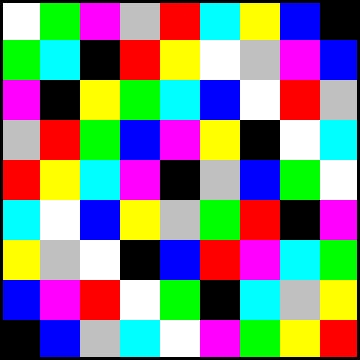
\includegraphics[width=5.5cm]{GRAPHICS/GF/GF_q9_addition_table_reordered_draw}
\qquad
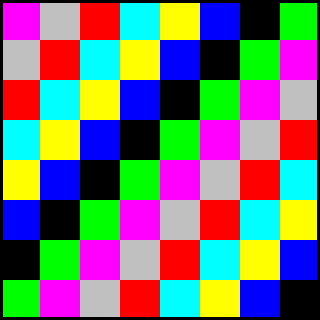
\includegraphics[width=5.5cm]{GRAPHICS/GF/GF_q9_multiplication_table_reordered_draw}
$$
\caption{\label{fig:fieldtables9rearranged}Addition and multiplication table 
of $\bbF_{9}$ using the cyclic ordering of elements}
\end{figure}


\bigskip

In Table~\ref{tab:linear:algebra}, some finite field activities regarding linear algebra are shown.
\begin{table}
	\begin{center}
	\begin{tabular}{|p{4cm}|p{3cm}|p{7cm}|}
		\hline
		Command & Arguments & Purpose \\
		\hline
		\hline
		\verb'-RREF' & $m$ $n$ $L$ & Compute the RREF of the $m \times n$ matrix $L$ over $\bbF_q$\\
		\hline
		\verb'-nullspace' & $m$ $n$ $L$  & Compute a basis for the right nullspace of the $m \times n$ matrix $L$\\
		\hline
		\verb'-normalize_from_' \verb'the_right' &  & Normalizes the result of \verb'-RREF' or \verb'nullspace' from the right\\
		\hline
		\verb'-normalize_from_' \verb'the_left' &  & Normalizes the result of \verb'-RREF' or \verb'nullspace' from the left\\
		\hline
		\verb'-eigenstuff' & $d$  $M$ & Computes the eigenvalues and eigenvectors of the given $d \times d$ matrix $M$ over $\bbF_q$\\
		\hline
		%\verb'-eigenstuff' \verb'_from_file' & $d$ fname & Computes the eigenvalues and eigenvectors of the  $d \times d$ matrix $M$ over $\bbF_q$. The matrix $M$ is read from a csv file.\\
		%\hline
		\verb'-all_rational' \verb'_normal_forms' & $d$   & Produces a report of all rational normal forms of endomorphisms of $\bbF_q^d$\\
		\hline
		\end{tabular}
	\end{center}
	\caption{\label{tab:linear:algebra}Finite Field Activities for Linear Algebra}
	\end{table}
For instance, the command
{\tt
\input GRAPHICS/THE_MAKEFILE/EXTRACTS/RREF.tex
}
computes the RREF form of the 
matrix 
$$
\left[
\begin{array}{ccccc}
1&1&1&1&0\\
1&1&0&0&1\\
\end{array}
\right]
$$
over $\bbF_2.$
The output is the matrix 
\begin{mdframed}[style=MyFrame]
$$
\left[
\begin{array}{*{5}{c}}
1 & 1 & 0 & 0 & 1\\
0 & 0 & 1 & 1 & 1\\
\end{array}
\right].
$$
\end{mdframed}

\bigskip

The \verb'-RREF' command produces a latex log of the steps. 
This can be used to follow the algorithm along. 
For a somewhat longer example, consider the Vandermonde matrix over the field $\bbF_7$.
Suppose we want to compute the inverse matrix directly. We can use the following command to do so. 
Notice how we first create the matrix and an identity matrix next to it. 
After that we apply the \verb'-RREF' command:
{\tt
\input GRAPHICS/THE_MAKEFILE/EXTRACTS/V7_VANDERMONDE_EXTENDED.tex
}
{\tt
\input GRAPHICS/THE_MAKEFILE/EXTRACTS/RREF_V7.tex
}
The following (shortened) output is produced. Observe how the inverse matrix 
appears in the second half once the \verb'-RREF' algorithm is finished: 
\begin{mdframed}[style=MyFrame]
\noindent A matrix over the field ${\mathbb F}_{7}$\\
$$
\left[
\begin{array}{*{14}{c}}
1 & 0 & 0 & 0 & 0 & 0 & 0 & 1 & 0 & 0 & 0 & 0 & 0 & 0\\
1 & 1 & 1 & 1 & 1 & 1 & 1 & 0 & 1 & 0 & 0 & 0 & 0 & 0\\
1 & 2 & 4 & 1 & 2 & 4 & 1 & 0 & 0 & 1 & 0 & 0 & 0 & 0\\
1 & 3 & 2 & 6 & 4 & 5 & 1 & 0 & 0 & 0 & 1 & 0 & 0 & 0\\
1 & 4 & 2 & 1 & 4 & 2 & 1 & 0 & 0 & 0 & 0 & 1 & 0 & 0\\
1 & 5 & 4 & 6 & 2 & 3 & 1 & 0 & 0 & 0 & 0 & 0 & 1 & 0\\
1 & 6 & 1 & 6 & 1 & 6 & 1 & 0 & 0 & 0 & 0 & 0 & 0 & 1\\
\end{array}
\right]
$$
\noindent  Position $(i,j)=(0,0),$ found pivot in column 0\\
$$
\left[
\begin{array}{*{14}{c}}
1 & 0 & 0 & 0 & 0 & 0 & 0 & 1 & 0 & 0 & 0 & 0 & 0 & 0\\
1 & 1 & 1 & 1 & 1 & 1 & 1 & 0 & 1 & 0 & 0 & 0 & 0 & 0\\
1 & 2 & 4 & 1 & 2 & 4 & 1 & 0 & 0 & 1 & 0 & 0 & 0 & 0\\
1 & 3 & 2 & 6 & 4 & 5 & 1 & 0 & 0 & 0 & 1 & 0 & 0 & 0\\
1 & 4 & 2 & 1 & 4 & 2 & 1 & 0 & 0 & 0 & 0 & 1 & 0 & 0\\
1 & 5 & 4 & 6 & 2 & 3 & 1 & 0 & 0 & 0 & 0 & 0 & 1 & 0\\
1 & 6 & 1 & 6 & 1 & 6 & 1 & 0 & 0 & 0 & 0 & 0 & 0 & 1\\
\end{array}
\right]
$$
\noindent After making pivot 1:\\
$$
\left[
\begin{array}{*{14}{c}}
1 & 0 & 0 & 0 & 0 & 0 & 0 & 1 & 0 & 0 & 0 & 0 & 0 & 0\\
1 & 1 & 1 & 1 & 1 & 1 & 1 & 0 & 1 & 0 & 0 & 0 & 0 & 0\\
1 & 2 & 4 & 1 & 2 & 4 & 1 & 0 & 0 & 1 & 0 & 0 & 0 & 0\\
1 & 3 & 2 & 6 & 4 & 5 & 1 & 0 & 0 & 0 & 1 & 0 & 0 & 0\\
1 & 4 & 2 & 1 & 4 & 2 & 1 & 0 & 0 & 0 & 0 & 1 & 0 & 0\\
1 & 5 & 4 & 6 & 2 & 3 & 1 & 0 & 0 & 0 & 0 & 0 & 1 & 0\\
1 & 6 & 1 & 6 & 1 & 6 & 1 & 0 & 0 & 0 & 0 & 0 & 0 & 1\\
\end{array}
\right]
$$

output truncated \\


\noindent After elimination above pivot 0 in position (0,0):\\
$$
\left[
\begin{array}{*{14}{c}}
1 & 0 & 0 & 0 & 0 & 0 & 0 & 1 & 0 & 0 & 0 & 0 & 0 & 0\\
0 & 1 & 0 & 0 & 0 & 0 & 0 & 0 & 6 & 3 & 2 & 5 & 4 & 1\\
0 & 0 & 1 & 0 & 0 & 0 & 0 & 0 & 6 & 5 & 3 & 3 & 5 & 6\\
0 & 0 & 0 & 1 & 0 & 0 & 0 & 0 & 6 & 6 & 1 & 6 & 1 & 1\\
0 & 0 & 0 & 0 & 1 & 0 & 0 & 0 & 6 & 3 & 5 & 5 & 3 & 6\\
0 & 0 & 0 & 0 & 0 & 1 & 0 & 0 & 6 & 5 & 4 & 3 & 2 & 1\\
0 & 0 & 0 & 0 & 0 & 0 & 1 & 6 & 6 & 6 & 6 & 6 & 6 & 6\\
\end{array}
\right]
$$
\end{mdframed}
The inverse matrix agrees with the output obtained in Section~\ref{sec:finite:fields}.



\bigskip


Another task is computing the nullspace of a matrix.
The command 
{\tt
\input GRAPHICS/THE_MAKEFILE/EXTRACTS/nullspace.tex
}
computes the right nullspace of the matrix from the first example.
The output is the matrix
\begin{mdframed}[style=MyFrame]
$$
\left[
\begin{array}{*{5}{c}}
1 & 0 & 0 & 1 & 1\\
0 & 1 & 0 & 1 & 1\\
0 & 0 & 1 & 1 & 0\\
\end{array}
\right].
$$
\end{mdframed}

\bigskip


Orbiter can compute eigenvalues and eigenvectors of matrices over finite fields. 
For instance, the command 
{\tt
\input GRAPHICS/THE_MAKEFILE/EXTRACTS/eigenstuff.tex
}
computes all eigenvectors and eigenvalues of the matrix
$$
\left[
\begin{array}{cccc}
	0&1&0&2\\
	0&1&2&1\\
	4&2&3&1\\
	2&0&4&3\\
\end{array}
\right]
$$
over $\bbF_5.$

\bigskip

Orbiter can produce a list of all conjugacy classes 
of endomorphisms of $\bbF_q^d$ by means of their rational normal forms. 
For instance
{\tt
\input GRAPHICS/THE_MAKEFILE/EXTRACTS/classes_GL_3_2.tex
}
produces a list of all conjugacy classes of $\GL(3,2).$
There are 6 of them.
The report includes the order of the centralizer and the order of the conjugacy class. 
The order of the centralizer is computed using Kung's formula~\cite{Kung81}.
This command relies on the Orbiter catalogue of irreducible polynomials.
For an introduction to the rational normal form of endomorphisms, see~\cite{Lueneburg1987}.
\begin{mdframed}[style=MyFrame]
\section*{Conjugacy Classes of ${\rm GL}(3,2)$}
The number of conjugacy classes of ${\rm GL}(3,2)$ is 6:\\
$$
\left[
\begin{array}{*{3}{r}}
         0 &          0 &          1\\
         1 &          0 &          1\\
         0 &          1 &          0\\
\end{array}
\right]
, 
\left[
\begin{array}{*{3}{r}}
         0 &          0 &          1\\
         1 &          0 &          0\\
         0 &          1 &          1\\
\end{array}
\right]
, 
\left[
\begin{array}{*{3}{r}}
         0 &          1 &          0\\
         1 &          1 &          0\\
         0 &          0 &          1\\
\end{array}
\right]
, 
\left[
\begin{array}{*{3}{r}}
         1 &          0 &          0\\
         1 &          1 &          0\\
         0 &          1 &          1\\
\end{array}
\right]
, 
\left[
\begin{array}{*{3}{r}}
         1 &          0 &          0\\
         1 &          1 &          0\\
         0 &          0 &          1\\
\end{array}
\right]
, 
$$
$$
\left[
\begin{array}{*{3}{r}}
         1 &          0 &          0\\
         0 &          1 &          0\\
         0 &          0 &          1\\
\end{array}
\right]
$$
\bigskip
Class 0 / 6\\
$3,1,0$
$$
\left[
\begin{array}{*{3}{r}}
         0 &          0 &          1\\
         1 &          0 &          1\\
         0 &          1 &          0\\
\end{array}
\right]$$
centralizer order $7$\\class size $24$\\
Class 1 / 6\\
$2,1,0$
$$
\left[
\begin{array}{*{3}{r}}
         0 &          0 &          1\\
         1 &          0 &          0\\
         0 &          1 &          1\\
\end{array}
\right]$$
centralizer order $7$\\class size $24$\\
Class 2 / 6\\
$0,1,0;1,1,0$
$$
\left[
\begin{array}{*{3}{r}}
         0 &          1 &          0\\
         1 &          1 &          0\\
         0 &          0 &          1\\
\end{array}
\right]$$
centralizer order $3$\\class size $56$\\
Class 3 / 6\\
$0,3,0$
$$
\left[
\begin{array}{*{3}{r}}
         1 &          0 &          0\\
         1 &          1 &          0\\
         0 &          1 &          1\\
\end{array}
\right]$$
centralizer order $4$\\class size $42$\\
Class 4 / 6\\
$0,3,1$
$$
\left[
\begin{array}{*{3}{r}}
         1 &          0 &          0\\
         1 &          1 &          0\\
         0 &          0 &          1\\
\end{array}
\right]$$
centralizer order $8$\\class size $21$\\
Class 5 / 6\\
$0,3,2$
$$
\left[
\begin{array}{*{3}{r}}
         1 &          0 &          0\\
         0 &          1 &          0\\
         0 &          0 &          1\\
\end{array}
\right]$$
centralizer order $168$\\class size $1$\\
\end{mdframed}
%Because the rational normal form is tied to irreducible polynomials, 
%this command relies on the built-in 
%knowledge base of irreducible polynomials in Orbiter. 
Let us now look at some advanced topics in the theory of finite fields. 


\bigskip


First, in Tables~\ref{tab:finite:field:activities:A}-\ref{tab:finite:field:activities:B},  a summary of 
finite field activities is shown.
\begin{table}
	\begin{center}
	\begin{tabular}{|p{4cm}|p{3cm}|p{7cm}|}
		\hline
		Command & Arguments & Purpose \\
		\hline
		\hline
		\verb'-write_code_' \verb'for_division' &  fname $A$ $B$ &  Write C++ source code for the polynomial division of $A$ by $B$. See Section~\ref{sec:CRC}.  \\
		\hline
		\verb'-polynomial_' \verb'division' &  $A$ $B$  &  Divides polynomial $B$ by polynomial $A$.  \\
		\hline
		\verb'-extended_gcd_' \verb'for_polynomials' &  $A$ $B$ &  Computes the extended gcd of polynomials $A$ and $B$.  \\
		\hline
		\verb'-polynomial_' \verb'mult_mod' &   $A$ $B$ $M$ &  Computes the product of polynomials $A$ and $B$ modulo the polynomial $M$.  \\
		\hline
		\verb'-polynomial_' \verb'power_mod' &   $A$ $N$ $M$ &  Computes the $n$-th power of the polynomial $A$ modulo the polynomial $M$.  \\
		\hline
		\verb'-Berlekamp_matrix' &  $A$ &  Compute the Berlekamp matrix associated with the polynomial $A$.  \\
		\hline
		\verb'-normal_basis' & $d$  &  Computes a normal basis for $\bbF_{q^d}$ over $\bbF_q$.  \\
		\hline
		\verb'-polynomial_' \verb'find_roots' & $A$  &  Computes the roots of the polynomial $A$.  \\
		\hline
		\verb'-nullspace' & $A$  &  Computes the right nullspace of the matrix $A$.  \\
		\hline
		\verb'-RREF' &  $A$ &  Computes the RREF of the matrix $A$.  \\
		\hline
		\verb'-weight_enumerator' & $A$  &  
		Computes the weight enumerator of the code whose generator matrix is $A$.  \\
		\hline
		\verb'-Walsh_Hadamard_' \verb'transform' & fname $n$  &  
		Computes the Walsh-Hadamard transform for the $n$-variable boolean function in the given file. \\
		\hline
		\verb'-algebraic_normal_' \verb'form' & fname $n$  &  
		Computes the algebraic normal form for the $n$-variable boolean function in the given file. \\
		\hline
		\verb'-apply_trace_' \verb'function' & fname   &  
		Applies the absolute trace function to the function in the given file. \\
		\hline
		\verb'-apply_power_' \verb'function' & fname $d$  &  
		Applies the raise-to-the-power-$d$ function to the function in the given file. \\
		\hline
		\verb'-identity_function' & fname\_csv   &  
		Creates the identity function and stores in the given csv file. \\
		\hline
		\verb'-Walsh_matrix' & $n$  &  Creates the Walsh matrix of order $n$. \\
		\hline
		\end{tabular}
	\end{center}
	\caption{\label{tab:finite:field:activities:A}Finite Field Activities (Part I)}
\end{table}
		
\begin{table}
	\begin{center}
	\begin{tabular}{|p{4cm}|p{3cm}|p{7cm}|}
		\hline
		Command & Arguments & Purpose \\
		\hline
		\hline
		\verb'-Vandermonde_matrix' & $n$  &  Creates the Vandermonde matrix of order $q \times q$. 
		The entry $(i,j)$ is $x_i^j$ where $w_0,\ldots,x_{q-1}$ is the list of field 
		elements in ordered according to the  Orbiter ranks.\\
		\hline
		\verb'-transversal' &  $L1$ $L2$ $P$ & 
		Computes the unique transversal to the lines $L1$ and $L2$ through the point $P$ in $\PG(3,q).$ 
		The linese are given by a basis consisting of $8$ field elements.  \\
		\hline
		\verb'-intersection_' \verb'of_two_lines' &  $L1$ $L2$ &  
		Computes the intersection of two lines in $\PG(3,q)$. 
		The linese are given by a basis consisting of $8$ field elements.  \\
		\hline
		\verb'-rank_point_in_PG' &  $P$ &  
		Computes the orbiter point rank of the point $P$ in $\PG(n,q).$ 
		$P$ is a label of a vector, which is the coefficient vector.  \\
		\hline
		\verb'-unrank_point_in_PG' &  $r$ &  
		Computes the orbiter point in $\PG(n,q)$ from the Orbiter rank value $r$.  \\
		\hline
		%\verb'-move_two_lines_' \verb'in_hyperplane_' \verb'stabilizer' &  $M1$ $M2$ $N1$ $N2$  &  Computes a projectivity  of $\PG(3,q)$ fixing the hyperplan $\bv(X_3)$ moving line $m_i$ to $n_i$ for $i=1,2.$ It assumes that both $m_1,m_2$ and $n_1,n_2$ are skew. The lines $m_i$ and $n_i$ are given through Orbiter line numbers.  \\
		%\hline
		%\verb'-move_two_lines_' \verb'in_hyperplane_' \verb'stabilizer_text' &  $M1$ $M2$ $N1$ $N2$ &  Like \verb'-move_two_lines_' \verb'in_hyperplane_stabilizer', but now each line is given by a $2 \times 4$ generator matrix for the subspace.  \\
		%\hline
		\verb'-inverse_isomor' \verb'phism_klein_quadric' & $L36$  &    \\
		\hline
		\verb'-NTT' &  $k$ $n$ &  Computes the Number-theoretic transform for $n=2^k,$ which must divide $q-1$. \\
		\hline
		\end{tabular}
	\end{center}
	\caption{\label{tab:finite:field:activities:B}Finite Field Activities (Part II)}
\end{table}

\bigskip




A normal basis for a field extension $\bbF_{q^d}$ over $\bbF_q$ 
is a basis of $\bbF_{q^d}$ as vector space over $\bbF_q$ 
which consists of one cycle of the Frobenius 
automorphism of $\bbF_{q^d}$ over $\bbF_q.$
For instance, the command
{\tt
\input GRAPHICS/THE_MAKEFILE/EXTRACTS/normal_basis_2_3.tex
}
computes a normal basis of $\bbF_8$ over $\bbF_2.$
Using the polynomial $X^{3} + X^{2} + 1,$
the normal basis in terms of the 
standard polynomial basis $1,X,X^2,\ldots$ 
is given by the columns of the matrix 
$$
\left[
\begin{array}{ccc}
1 &0 &0\\ 
1 &1 &0 \\
1 &0 &1 \\
\end{array}
\right].
$$
Reading the columns as cofficient vectors with respect to the standard basis, 
the normal basis is 
$$
b_1 = 1 + X + X^2, \quad b_2 = X, \quad b_3 = X^2.
$$
Let us apply the Frobenius mapping $\Phi$ to the elements of the normal bases:
\begin{align*}
b_1^\Phi &= (1+X+X^2)^2 = 1 + X^2 + X^4 = 1 + X^2 + X^3 + X = 1 + X + X^2 + X^2 + 1 = X = b_2,\\
b_2^\Phi &= X^2 = b_3, \\
b_3^\Phi &= X^4 = X^3+X = X^2+X+1 = b_1.
\end{align*}
Thus,
$$
b_1 \mapsto b_2 \mapsto b_3 \mapsto b_1
$$ 
under $\Phi,$ as required.

\bigskip

A field is a vector space over any of its subfields. 
Using a field basis, the elements of the large field can be 
identified with invertible matrices. 
So, for $\bbF_{q^r}$ over $\bbF_q$, and for $a \in \bbF_{q^r},$ 
we consider the $\bbF_q$-linear map 
$$
\bbF_{q^r} \rightarrow \bbF_{q^r} , x \mapsto ax.
$$
The following code computes the field reduction from $\bbF_{64}$ to $\bbF_8$. 
Elements in the small field are represented as colors.
The $(i,j)$-th block is the matrix of $a=i8+j$ in the chosen basis.
{\tt
\input GRAPHICS/THE_MAKEFILE/EXTRACTS/F_64_over_F8_field_reduction.tex
}
The output is shown in Figure~\ref{fic:field:reduction:64:8}.
\begin{figure}
$$
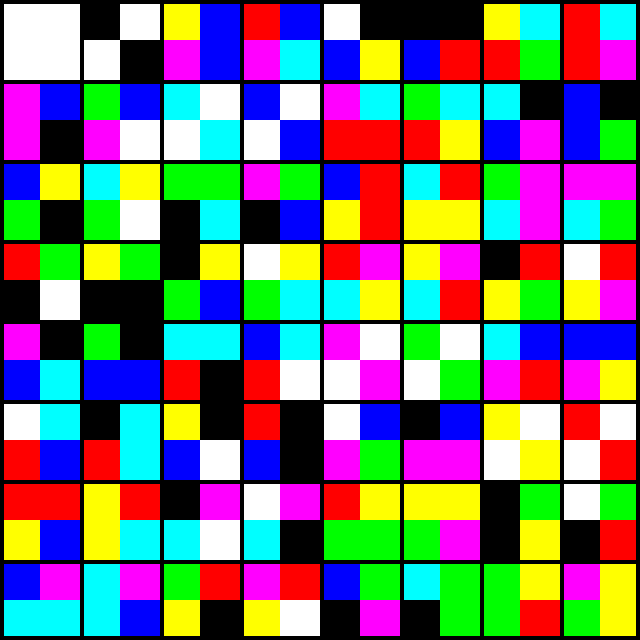
\includegraphics[width=8cm]{GRAPHICS/FIELD_REDUCTION/F64_over_F8_draw}
$$
\caption{\label{fic:field:reduction:64:8}The field reduction from $\bbF_{64}$ to $\bbF_8$}
\end{figure}
Note that the dimension of the vector space is 2, so the block matrices are $2 \times 2.$
Observe that $\bbF_{64}$ has many subfields. 
Figure~\ref{fic:field:reduction:64:4} shows the field reduction from 
$\bbF_{64}$ to $\bbF_4$ (left) and from 
$\bbF_{64}$ to $\bbF_2$ (right).
\begin{figure}
$$
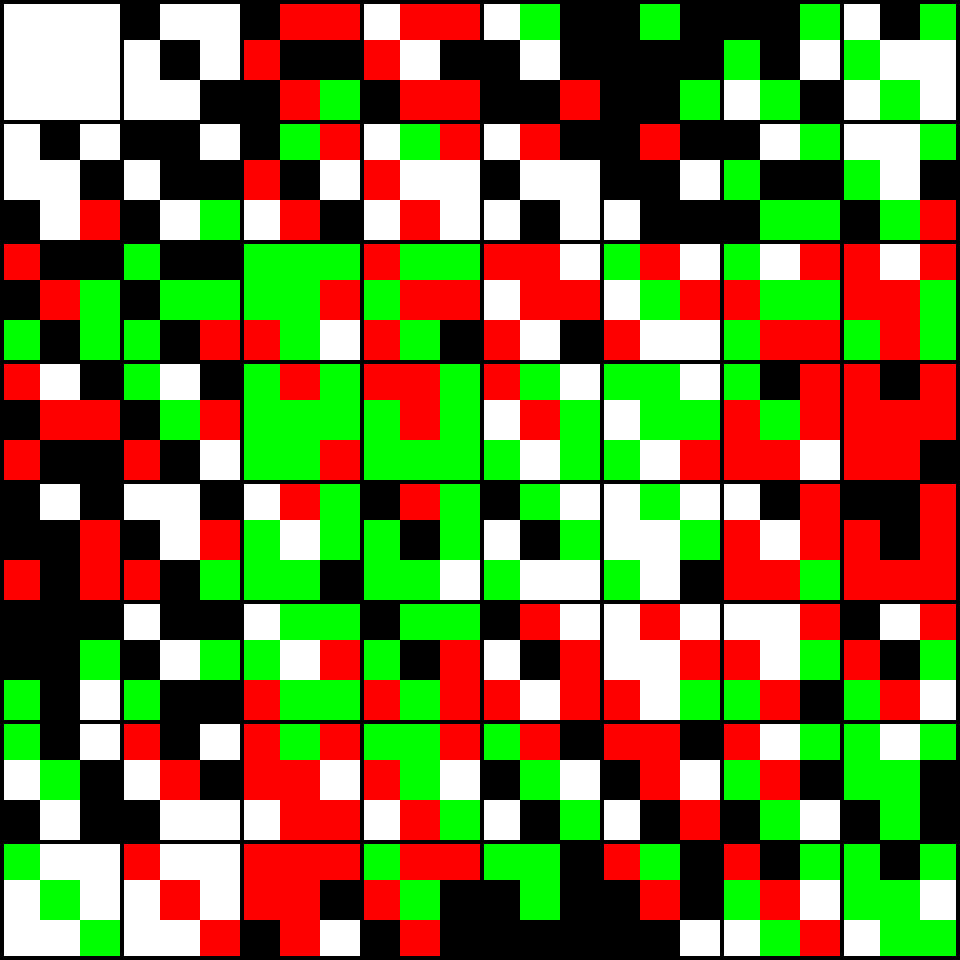
\includegraphics[width=8cm]{GRAPHICS/FIELD_REDUCTION/F64_over_F4_draw}
\;
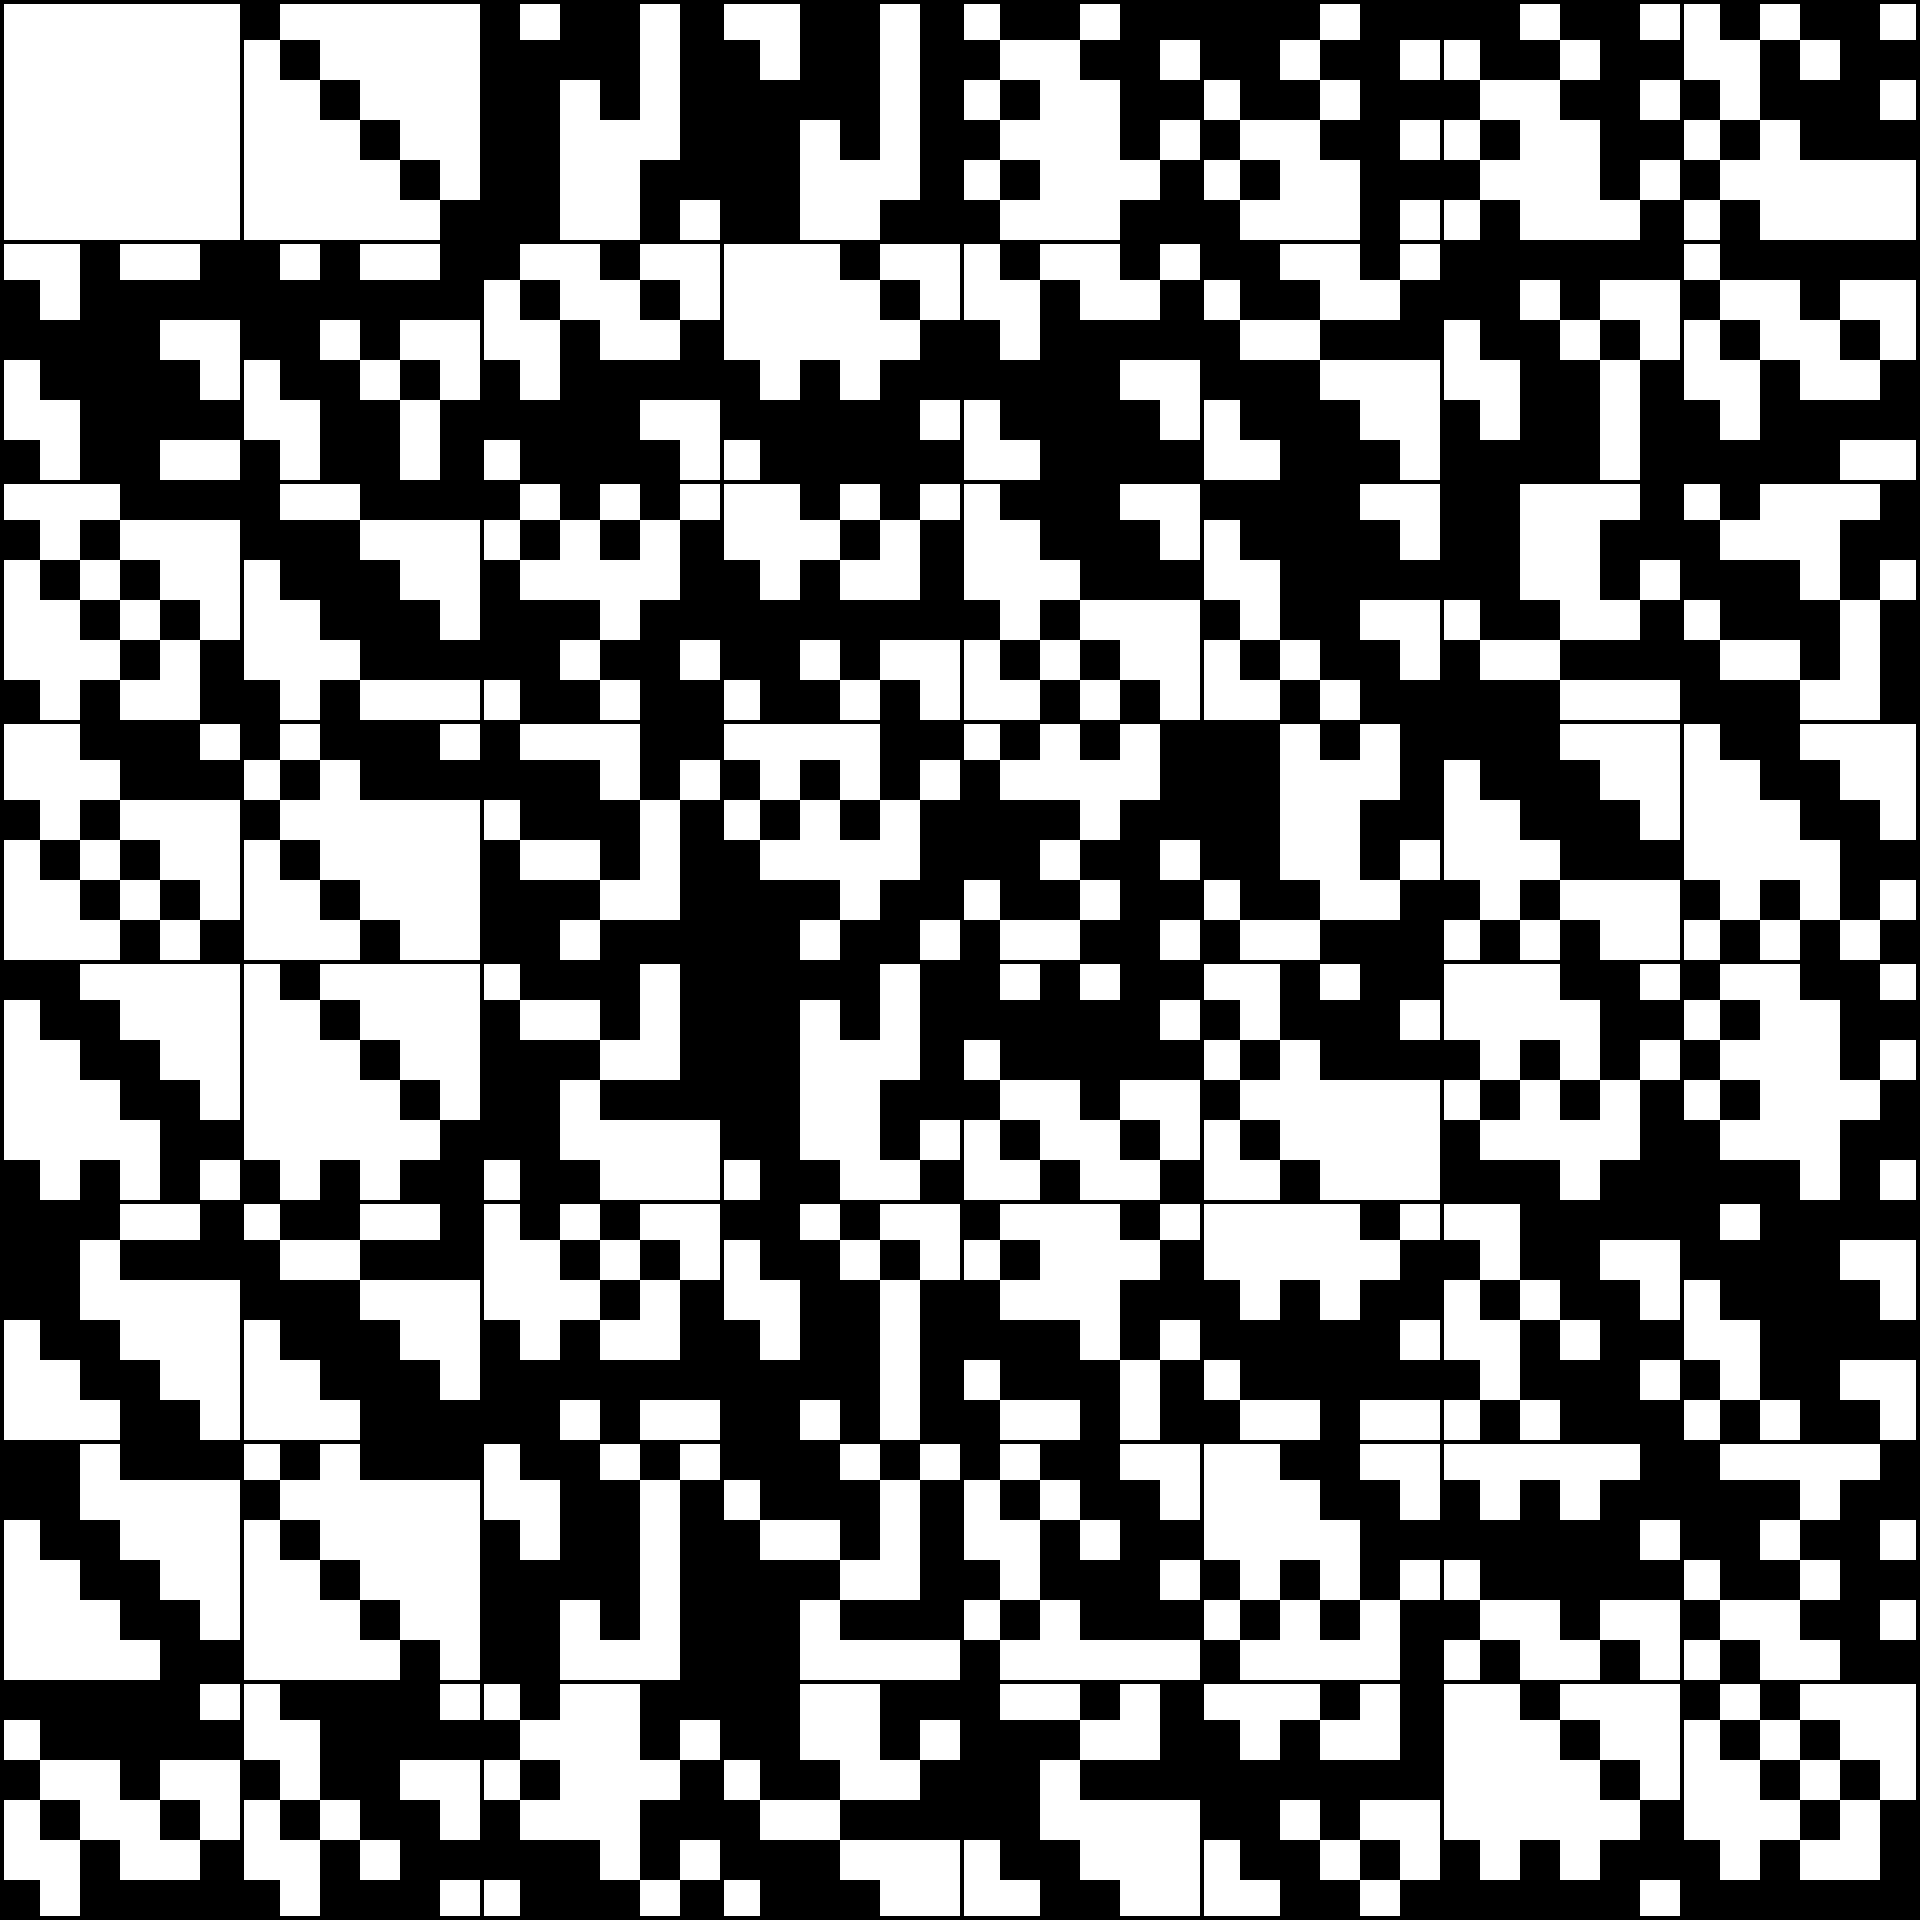
\includegraphics[width=8cm]{GRAPHICS/FIELD_REDUCTION/F64_over_F2_draw}
$$
\caption{\label{fic:field:reduction:64:4}The field reduction from $\bbF_{64}$ to $\bbF_4$ (left) and from $\bbF_{64}$ to  $\bbF_2$ (right)}
\end{figure}
Here, the block matrices have size $3 \times 3$ and $6 \times 6$, respectively.

\bigskip

The minimum polynomials associated with the $n$-th roots 
over $\bbF_q$ can be computed using the \verb'-nth_roots' command, which is a 
finite field activity. 
The activity is aplied to the field $\bbF_q$ over which the $n$-th roots are defined.
The command constructs the filed extension $\bbF_{q^m}$ where $m$ is the order of $q$ modulo $n$. 
This field extension contains the $n$-th roots of unity. 
Let $\alpha$ be a primitive element of $\bbF_{q^m}$ and let $\beta$ be a generator of the subgroup of $n$-th roots. 
Also, let $\gamma$ be the generator of the subgroup of $q-1$ th roots, which are the elements of the multiplicative group of $\bbF_q.$ 
The output lists the $n$-th roots first, generated by $\beta$. After that, the $q-1$th roots are shown, generated by $\gamma$. 
Finally, a table is produced which shows the irreducible polynomials over $\bbF_q$ associated with the $n$-th roots of unity.
For instance, the following command computes the minimum polynomials of all $21$st roots of unity over $\bbF_8$:
{\tt
\input GRAPHICS/THE_MAKEFILE/EXTRACTS/F_8_Nth_roots_21.tex
}
The output is:
\begin{mdframed}[style=MyFrame]

\noindent Let $\alpha$ be a primitive element of GF$(64)$. 
Let $\beta$ be a primitive $21$-th root in GF$(64)$, 
so $\beta=\alpha^{3}.$ \\
$\beta^{0} = 100000 =  1$\\
$\beta^{1} = 000100 =  \alpha^{3}$\\
$\beta^{2} = 100001 =  \alpha^{5} + 1$\\
$\beta^{3} = 111101 =  \alpha^{5} + \alpha^{3} + \alpha^{2} + \alpha + 1$\\
$\beta^{4} = 011111 =  \alpha^{5} + \alpha^{4} + \alpha^{3} + \alpha^{2} + \alpha$\\
$\beta^{5} = 101010 =  \alpha^{4} + \alpha^{2} + 1$\\
$\beta^{6} = 110100 =  \alpha^{3} + \alpha + 1$\\
$\beta^{7} = 100111 =  \alpha^{5} + \alpha^{4} + \alpha^{3} + 1$\\
$\beta^{8} = 101101 =  \alpha^{5} + \alpha^{3} + \alpha^{2} + 1$\\
$\beta^{9} = 011101 =  \alpha^{5} + \alpha^{3} + \alpha^{2} + \alpha$\\
$\beta^{10} = 011011 =  \alpha^{5} + \alpha^{4} + \alpha^{2} + \alpha$\\
$\beta^{11} = 001011 =  \alpha^{5} + \alpha^{4} + \alpha^{2}$\\
$\beta^{12} = 001001 =  \alpha^{5} + \alpha^{2}$\\
$\beta^{13} = 111000 =  \alpha^{2} + \alpha + 1$\\
$\beta^{14} = 000111 =  \alpha^{5} + \alpha^{4} + \alpha^{3}$\\
$\beta^{15} = 101001 =  \alpha^{5} + \alpha^{2} + 1$\\
$\beta^{16} = 111100 =  \alpha^{3} + \alpha^{2} + \alpha + 1$\\
$\beta^{17} = 100110 =  \alpha^{4} + \alpha^{3} + 1$\\
$\beta^{18} = 010100 =  \alpha^{3} + \alpha$\\
$\beta^{19} = 100011 =  \alpha^{5} + \alpha^{4} + 1$\\
$\beta^{20} = 001100 =  \alpha^{3} + \alpha^{2}$\\
\bigskip

\noindent Let $\gamma$ be a primitive $7$-th root in GF$(64)$, 
so $\gamma=\alpha^{9}.$ \\
$\gamma^{0} = 100000 = 1$\\
$\gamma^{1} = 111101 = \alpha^{5} + \alpha^{3} + \alpha^{2} + \alpha + 1$\\
$\gamma^{2} = 110100 = \alpha^{3} + \alpha + 1$\\
$\gamma^{3} = 011101 = \alpha^{5} + \alpha^{3} + \alpha^{2} + \alpha$\\
$\gamma^{4} = 001001 = \alpha^{5} + \alpha^{2}$\\
$\gamma^{5} = 101001 = \alpha^{5} + \alpha^{2} + 1$\\
$\gamma^{6} = 010100 = \alpha^{3} + \alpha$\\
\bigskip

\noindent The $q$-cyclotomic set for $q=8$ are:

\noindent $\{$ 0 $\}$\\
$\{$ 1, 8 $\}$\\
$\{$ 2, 16 $\}$\\
$\{$ 3 $\}$\\
$\{$ 4, 11 $\}$\\
$\{$ 5, 19 $\}$\\
$\{$ 6 $\}$\\
$\{$ 7, 14 $\}$\\
$\{$ 9 $\}$\\
$\{$ 10, 17 $\}$\\
$\{$ 12 $\}$\\
$\{$ 13, 20 $\}$\\
$\{$ 15 $\}$\\
$\{$ 18 $\}$\\
\bigskip

Subfield basis, a basis for GF$(8)$ inside GF$(64)$:
$$
\left[
\begin{array}{*{6}{c}}
1 & 0 & 0 & 0 & 0 & 0\\
1 & 1 & 1 & 1 & 0 & 1\\
1 & 1 & 0 & 1 & 0 & 0\\
\end{array}
\right]
$$
\bigskip

The irreducible polynomials associated with the $21$-th roots over GF$(8)$ are:

\bigskip


{\renewcommand{\arraystretch}{1.5}
$$
\begin{array}{|r|r|l|l|l|}
\hline
i & r_i & {\rm Cyc}(r_i) & m_{\beta^{r_i}}(X) & m_{\beta^{r_i}}(X) \\
\hline
0 & 0 & ( 0 ) & (100000)  X^{0} + (100000)  X^{1} & X + 1\\
\hline
1 & 1 & ( 1, 8 ) & (011101)  X^{0} + (101001)  X^{1} + (100000)  X^{2} & X^{2} + 7X + 3\\
\hline
2 & 2 & ( 2, 16 ) & (010100)  X^{0} + (011101)  X^{1} + (100000)  X^{2} & X^{2} + 3X + 5\\
\hline
3 & 3 & ( 3 ) & (111101)  X^{0} + (100000)  X^{1} & X + 2\\
\hline
4 & 4 & ( 4, 11 ) & (101001)  X^{0} + (010100)  X^{1} + (100000)  X^{2} & X^{2} + 5X + 7\\
\hline
5 & 5 & ( 5, 19 ) & (111101)  X^{0} + (001001)  X^{1} + (100000)  X^{2} & X^{2} + 6X + 2\\
\hline
6 & 6 & ( 6 ) & (110100)  X^{0} + (100000)  X^{1} & X + 4\\
\hline
7 & 7 & ( 7, 14 ) & (100000)  X^{0} + (100000)  X^{1} + (100000)  X^{2} & X^{2} + X + 1\\
\hline
8 & 9 & ( 9 ) & (011101)  X^{0} + (100000)  X^{1} & X + 3\\
\hline
9 & 10 & ( 10, 17 ) & (110100)  X^{0} + (111101)  X^{1} + (100000)  X^{2} & X^{2} + 2X + 4\\
\hline
10 & 12 & ( 12 ) & (001001)  X^{0} + (100000)  X^{1} & X + 6\\
\hline
11 & 13 & ( 13, 20 ) & (001001)  X^{0} + (110100)  X^{1} + (100000)  X^{2} & X^{2} + 4X + 6\\
\hline
12 & 15 & ( 15 ) & (101001)  X^{0} + (100000)  X^{1} & X + 7\\
\hline
13 & 18 & ( 18 ) & (010100)  X^{0} + (100000)  X^{1} & X + 5\\
\hline
\end{array}
$$}
\end{mdframed}


\bigskip

In Section~\ref{sec:finite:fields}, we considered the Vandermonde matrix over $\bbF_7$. 
Let us do the same for the field $\bbF_8$ instead. We use the following command:
{\tt
\input GRAPHICS/THE_MAKEFILE/EXTRACTS/F_8_vandermonde.tex
}
The output is shown below. Again, the first matrix is $V = (x_{i}^j).$ The second matrix is $V^{-1}$:
\begin{mdframed}[style=MyFrame]
$$
\left[
\begin{array}{*{8}{c}}
1 & 0 & 0 & 0 & 0 & 0 & 0 & 0\\
1 & 1 & 1 & 1 & 1 & 1 & 1 & 1\\
1 & 2 & 4 & 5 & 7 & 3 & 6 & 1\\
1 & 3 & 5 & 2 & 6 & 7 & 4 & 1\\
1 & 4 & 7 & 6 & 2 & 5 & 3 & 1\\
1 & 5 & 6 & 4 & 3 & 2 & 7 & 1\\
1 & 6 & 3 & 7 & 5 & 4 & 2 & 1\\
1 & 7 & 2 & 3 & 4 & 6 & 5 & 1\\
\end{array}
\right]
, \qquad
\left[
\begin{array}{*{8}{c}}
1 & 0 & 0 & 0 & 0 & 0 & 0 & 0\\
0 & 1 & 6 & 4 & 3 & 7 & 2 & 5\\
0 & 1 & 3 & 7 & 5 & 2 & 4 & 6\\
0 & 1 & 7 & 6 & 2 & 3 & 5 & 4\\
0 & 1 & 5 & 2 & 6 & 4 & 7 & 3\\
0 & 1 & 4 & 5 & 7 & 6 & 3 & 2\\
0 & 1 & 2 & 3 & 4 & 5 & 6 & 7\\
1 & 1 & 1 & 1 & 1 & 1 & 1 & 1\\
\end{array}
\right]
$$
\end{mdframed}

\bigskip


Let us now do a somewhat larger example of the same problem. 
The next command computes the Vandermonde matrix and its inverse over the field 
$\bbF_{1024}$:
{\tt
\input GRAPHICS/THE_MAKEFILE/EXTRACTS/F_1024_vandermonde.tex
}
This command takes a bit of time to execute. The matrix is not shown. It would be too big to be printed.
In order to save disc space, we delete the output files, using the \verb'rm' command.

\bigskip






Orbiter can create code for the number theoretic transform. 
This is the discrete Fourier transform performed over finite fields.
The generated code can be compiled with the Orbiter library. 
Compiling code requires additional makefile options are necessary. 
Because of this, we define the following makefile variables 
at the top of the makefile.
{\tt
\input GRAPHICS/THE_MAKEFILE/EXTRACTS/SRC.tex
}

\bigskip

Suppose we want to create 
the number theoretic transform for the 16th 
roots of unity inside the field $\bbF_{17}.$ 
Here is the command to generate the Orbiter source code:
{\tt
\input GRAPHICS/THE_MAKEFILE/EXTRACTS/NTT_k4_q17.cpp.tex
}
This produces a C++ file \verb'NTT_k4_q17.cpp'. 
This file should be compiled and linked against the Orbiter library. 
The command 
{\tt
\input GRAPHICS/THE_MAKEFILE/EXTRACTS/F_17_NTT_compile.tex
}
can be used to compile the code and run it. 
Note the dependency on the file \verb'NTT_k4_q17.cpp'. 
This means that \verb'make' would automatically 
invoke the first command if only the second one was issued.

 











Orbiter can deal with multivariate polynomial rings with coefficients 
over finite fields.
Orbiter creates the homogenous components only (so it is technically not a ring).

\bigskip


The following command creates the homogeneous component of degree 3 in 
a polynomial ring in 4 variables. 
The variables are named. They are $x_0,x_1,x_2,x_3.$ 
Note that two sets of names are defined using the \verb'-variables' command. 
The first is the labels for regular text output. 
The second is the set of names for latex output.
Here is the command:
{\tt
\input GRAPHICS/THE_MAKEFILE/EXTRACTS/Polynomial_ring.tex
}

\bigskip

For more on rings, see Chapter~\ref{chapter:ring:theory}.

\section{Finite Projective Spaces}
\label{sec:FPG}


\input C04/sec_1.tex



\bigskip

\clearpage


\section{Indexing Points and Lines}
\label{sec:indexing:points}


\input C04/sec_2.tex



\bigskip

\clearpage




\section{Finite Desarguesian Projective Planes}
\label{sec:finite:desarguesian:planes}


\input C04/sec_3.tex



\bigskip

\clearpage


\section{The Grassmannian}
\label{sec:grassmannian}


\input C04/sec_4.tex



\bigskip

\clearpage


\section{Algebraic Sets}
\label{sec:algebraicsets}



\input C04/sec_5.tex




\clearpage


\section{The Klein Quadric and the Pl\"ucker Map}
\label{sec:klein}


\input C04/sec_6.tex



\bigskip

\clearpage


\section{Orthogonal Spaces}
\label{sec:orthogonal}


\input C04/sec_7.tex



\bigskip

\clearpage


\section{Hermitian Varieties}
\label{sec:hermitian}


\input C04/sec_8.tex



\bigskip

\clearpage


\section{Advanced Topics}
\label{sec:advanced:topics}


\input C04/sec_9.tex



\bigskip

\clearpage


\section{Geometric Objects}
\label{sec:geometric:objects}


\input C04/sec_10.tex



\bigskip

\clearpage

Orbiter can create the projective space $\PG(n,q).$ 
In order to do so, an object of type projective\_space needs to be defined. 
Once the object exists, various commands are available. 
Let us look at a very simple example. 
Suppose we want to create $\PG(3,2).$ 
The following command sequence first creates the finite field $\bbF_2.$
The symbol $F$ is used to store the field.
After that, the projective space $\PG(3,F)$ is created and stored in the symbol $P$.
No other commands are given:
{\tt
\input GRAPHICS/THE_MAKEFILE/EXTRACTS/PG_3_2_easy.tex
}

\bigskip





This means that Orbiter offers indexing for the subspaces of $\PG(n,q)$ of a fixed dimension. 
For instance, there are enumerators for points and lines. 
Besides these, there are enumerators for subspaces of any dimension.
The incidence matrix between points and lines with respect to this ordering can be 
computed. 
The indexing is used to establish the permutation representations of the projective group, 
as will be described in Section~\ref{sec:lineargroups}.
The indexing of points is not the lexicographic ordering. 
It emphasizes the role of frames in the geometry
by assigning the smallest rank values to the members of th standard frame. 
After that, the other points are listed. 

\bigskip


Orbiter can create cheat sheets, 
which summarize the properties of $\PG(n,q)$ and list the various elements. 
The following command creates a cheat sheet for $\PG(2,4)$ using a finite field object:
{\tt
\input GRAPHICS/THE_MAKEFILE/EXTRACTS/PG_2_4.tex
}
The cheat sheet contains a drawing of the plane as shown in Figure~\ref{fig:PG24}.
\begin{figure}
$$
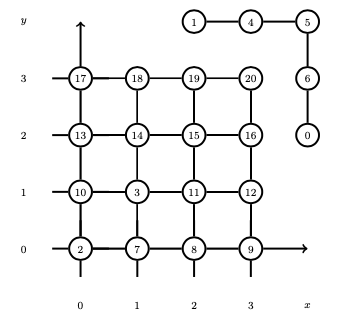
\includegraphics[width=9cm]{GRAPHICS/PG/PG_2_4}
%
\includegraphics[width=7cm]{GRAPHICS/PG_2_4_pic}
$$
\caption{\label{fig:PG24}The plane $\PG(2,4)$}
\end{figure}
The affine plane is shown in the cartesian plane, 
while the line at infinity is wrapped around the top right corner.
The cheat sheet continues by listing the points, including the 
canonical Baer subgeometry $\PG(2,2).$
After that, the points are listed again, but with left-normalized vectors.
Finally, the lines are shown. 
\begin{mdframed}[style=MyFrame]
\input GRAPHICS/LATEX/report_PG_2_4.tex
\end{mdframed}



\bigskip

Here is a slightly larger example. The following command creates a cheat sheet for $\PG(3,2).$
{\tt
\input GRAPHICS/THE_MAKEFILE/EXTRACTS/PG_3_2.tex
}
The cheat sheet shows points, lines and planes. 
The lines are shown together with their Pl\"ucker coordinates. 
The lines whose Pl\"ucker coordinates are unit vectors are shown separately.
\begin{mdframed}[style=MyFrame]
\input GRAPHICS/LATEX/report_PG_3_2.tex
\end{mdframed}

\bigskip





Orbiter can create objects in projective space.
To do so, define an object of type
\verb'-geometric_object'.
The definition of a geometric object requires a projective geometry object. 
For this reason, the definition requires an extra argument, 
which is the label of a previously created projective geometry object.
After that, one of the commands shown in Tables~\ref{tab:objects} and~\ref{tab:objects2} can be issued.
Modifier options as shown in Table~\ref{tab:objects:modifiers} apply.
\begin{table}
\begin{center}
\begin{tabular}{|p{4cm}|l|p{8cm}|}
\hline
Command  & Arguments & Purpose \\
\hline
\hline
\verb'-hyperoval' &  & To create a hyperoval  \\
\hline
\verb'-subiaco_oval' & f\_short & Create the Subiaco oval  \\
\hline
\verb'-subiaco_hyperoval' &  & Create the Subiaco hyperoval  \\
\hline
\verb'-adelaide_hyperoval' &  & Create the Adalaide hyperoval  \\
\hline
\verb'-translation' & $i$ & Create the translation hyperoval with exponent $i$ \\
\hline
\verb'-Segre' &  & Create the Segre hyperoval  \\
\hline
\verb'-Payne' &  & Create the Payne hyperoval  \\
\hline
\verb'-Cherowitzo' &  & Create the Cherowitzo hyperoval  \\
\hline
\verb'-OKeefe_Penttila' &  & Create the O'Keefe, Penttila hyperoval  \\
\hline
\verb'-BLT_database' & $k$ & Create the $k$th BLT-set of order $q$ from the database ($k=0,1,\ldots$) \\
\hline
		\verb'-elliptic_quadric_' \verb'ovoid' &  &  Create an elliptic quadric ovoid in $\PG(3,q)$. \\
		\hline
		\verb'-ovoid_ST' &  &  Create the Suzuki Tits ovoid in $\PG(3,q)$. Here, $q=2^{2r+1}.$ \\
		\hline
\verb'-Baer' &  & Create the (standard) Baer subgeometry \\
\hline
\verb'-orthogonal' & $\epsilon$ & Create the $Q^\epsilon(n,q)$ quadric \\
\hline
\verb'-hermitian' & & Create the Hermitian variety given by $\sum_{i=0}^n X_i^{\sqrt{q}+1} = 0$\\
\hline
\verb'-cuspidal_cubic' & & Create the cuspidal cubic $(s^3,ts^2,t^3)$ in $\PG(2,q)$\\
\hline
\verb'-twisted_cubic' & & Create a twisted cubic $(s^3,s^2t,st^2,t^3)$ in $\PG(3,q)$\\
\hline
\verb'-elliptic_curve' & $a$ $b$ & Create the elliptic curve $y^2=x^3+ax+b$ \\
\hline
\verb'-ttp_construc' \verb'tion_A' &  & Create the twisted tensor product code of type $A$~\cite{Betten2008} \\
\hline
\verb'-ttp_construc' \verb'tion_A_hyperoval' &  & Create the twisted tensor product code of type $A$~\cite{Betten2008} \\
\hline
\verb'-ttp_construc' \verb'tion_B' &  & Create the twisted tensor product code of type $B$~\cite{Betten2008} \\
\hline
\end{tabular}
\end{center}
\caption{\label{tab:objects}Orbiter Objects (Part 1)}
\end{table}
\begin{table}
\begin{center}
\begin{tabular}{|p{4cm}|l|p{8cm}|}
\hline
Command  & Arguments & Purpose \\
\hline
\hline
\verb'-unital_' \verb'XXq_YZq_ZYq' &  &  Create  the unital with equation $XX^q+YZ^q+ZY^q=0$ \\
\hline
\verb'-desarguesian_' \verb'line_spread_' \verb'in_PG_3_q' &  & Create the desarguesian line spread in $\PG(3,q)$ as a set of 2-subspaces \\
\hline
\verb'-Buekenhout_Metz' &  & Create the Buekenhout Metz unital \\
\hline
\verb'-Uab' & $a$ $b$ & Create the Buekenhout Metz unital in the form of Barwick and Ebert~\cite{BarwickEbert2008}\\
\hline
\verb'-whole_space' &  & Create the whole space\\
\hline
\verb'-hyperplane' & pt & Create the hyperplane given by dual coordinates associated with the given point\\
\hline
\verb'-segre_variety' & $a$ $b$ & Create the Segre variety\\
\hline
\verb'-Maruta_Hamada_arc' &  & Create the Maruta Hamada arc\\
\hline
		\verb'-projective_variety' & lab\_ascii lab\_tex $d$ coeffs & 
		Create a projective variety of degree $d$ from an equation. 
		By default, the coefficients of the equation are listed in the partition ordering. 
		A different ordering can be specified. 
		A label for the variety in ascii and in tex is required. See Section~\ref{sec:algebraicsets}. \\
\hline
\verb'-intersection_of_' \verb'zariski_open_sets' & $l$ $d$ $n$ $\cC_1$ ... $\cC_n$ & Create the intersection of the Zariski open sets given by equations $\cC_1,\ldots\cC_n$ of degree $d$ with label $l$, see Section~\ref{sec:algebraicsets}. \\
\hline
\verb'-projective_curve' & $l$ $r$ $d$ $\cC$ & Create the projective curve of degree $d$ with label $l$, 
with coefficient vector $\cC$ in $r$ variables\\
\hline
\end{tabular}
\end{center}
\caption{\label{tab:objects2}Orbiter Objects (Part 2)}
\end{table}
\begin{table}
\begin{center}
\begin{tabular}{|p{4cm}|l|p{8cm}|}
\hline
Command  & Arguments & Purpose \\
\hline
\hline
\verb'-embedded_in_PG_4_q' &  &  \\
\hline
\verb'-BLT_in_PG' &  & Create the BLT-set with ranks in $\PG(n,q)$ instead of orthogonal point ranks \\
\hline
		\verb'-monomial_type_LEX' &  &  Select lexicographic ordering of coefficients in an algebraic equation. \\
		\hline
		\verb'-monomial_type_PART' &  &  Select partition ordering of coefficients in an algebraic equation (default). \\
		\hline
\end{tabular}
\end{center}
\caption{\label{tab:objects:modifiers}Orbiter Objects: Modifiers}
\end{table}





The following command creates an elliptic quadric ovoid on $\PG(3,8)$:
{\tt
\input GRAPHICS/THE_MAKEFILE/EXTRACTS/elliptic_quadric_ovoid_q8.tex
}
The next command creates the Suzuki-Tits ovoid in $\PG(3,8)$:
{\tt
\input GRAPHICS/THE_MAKEFILE/EXTRACTS/ovoid_ST_q8.tex
}
The Edge curve is given by the equation
$$
X^4 -Y^4 -Z^4 +2f^2Y^2Z^2 +4fX^2YZ =0
$$
where $f$ is a primitive element of $\bbF_q.$
Let us pick $q=17.$
The next example creates the Edge curve in $\PG(2,17)$ and saves it to file. 
The equation is encoded using the ordering of quartic monomials 
from Table~\ref{tab:PG2monomials}.
{\tt
\input GRAPHICS/THE_MAKEFILE/EXTRACTS/EDGE_CURVE_Q17_EQUATION.tex
}
{\tt
\input GRAPHICS/THE_MAKEFILE/EXTRACTS/EDGE_CURVE_Q17_AS_POINTS.tex
}
{\tt
\input GRAPHICS/THE_MAKEFILE/EXTRACTS/FILE_Q17.tex
}
{\tt
\input GRAPHICS/THE_MAKEFILE/EXTRACTS/Edge_curve_17.tex
}
The following command computes the line type of the Edge curve:
{\tt
\input GRAPHICS/THE_MAKEFILE/EXTRACTS/Edge_curve_17_line_type.tex
}
The line type is 
$$
( 4^6, 2^{30}, 1^{132}, 0^{139} )
$$
This means that there are 6 4-secants, 
30 2-secants, 132 tangent lines, and 139 external lines to the curve.




The enumerator for points establishes a bijection between 
the set of points and the integers on the 
interval $[0,\theta_n(q)-1],$ 
where 
$$
\theta_n(q) = \frac{q^{n+1}-1}{q-1}.
$$
In order to facilitate the bijection, 
Orbiter enumerates representative vectors 
for the one-dimensional subspaces.
The conditions on the vectors are summarized below:
\begin{enumerate}
\item
The vector is not the zero vector.
\item
The rightmost nonzero entry in the vector is one. 
If it is not, we nomalize the vector 
so that the rightmost nonzero vector is indeed one. 
This operation does not change the projective 
point which is associated with the vector.
\end{enumerate}
The second condition ensures that we list 
each projective point exactly once.
We require two functions, 
{\sc Rank} and {\sc Unrank}. The function {\sc Rank} takes a vector 
$\bx \in \bbF_q^n,$ 
not zero, and maps it to the element in $\bbZ_N$ 
representing the projective point 
$\bP(\bx).$
A frame in $\PG(n,q)$ is a set of $n+2$ points, no $n+1$ in a hyperplane. 
We assume that the coordinates of a vector 
are indexed by the elements of $\bbZ_n.$ 
Also, we let $\be_i$ be the $i$-th unit vector. 
A frame for $\PG(n,q)$ is  
$$
\be_0,\ldots,\be_{n-1}, \be_0+\cdots+\be_{n-1}.
$$
This is the {\em standard frame.} 
We start the labeling of points with the  
standard frame. After these $n+2$ points, 
we list the remaining points 
in lexicographic ordering (utilizing right-normalized representative).
Thus, for $\PG(2,2)$ the  ordering is
\begin{center}
$(1,0,0),$
$(0,1,0),$
$(0,0,1),$
$(1,1,1),$
$(1,1,0),$
$(1,0,1),$
$(0,1,1).$
\end{center}
Let us describe the two functions rank and unrank 
to perform the actual mappings 
between $\PG(n,q)$ and $\bbZ_{N},$ where $N = \theta_n(q).$
For this, assume that ranking and unranking 
functions have already been defined for the 
elements of the finite field $\bbF_q$.
Thus, we assume that for $x \in \bbF_q$, 
{\sc Rank}$(\bbF_q,x)$ is a number $b$ in $\bbZ_q.$
Also, for $b \in \bbZ_q$, 
we assume that {\sc Unrank}$(\bbF_q,b)$ is the 
corresponding $x \in \bbF_q$.
So, we assume that 
{\sc Rank} and {\sc Unrank} are mutually inverse functions.  
\begin{algorithm}
\caption{Rank}\label{algo:Rank}
\begin{algorithmic}[1]
\Procedure{Rank}{\textbf{vector} : $\bx,$ \textbf{field} : $\bbF_q$, $\textbf{int} : n$}
\State \textbf{assert} $\bx$ is a nonzero vector in $\bbF_q^n.$
\If {$\bx = \be_i$} 
\State \Return $i$
\EndIf
\If {$\bx = \bone$} 
\State \Return $n$
\EndIf
\State $i \gets \max\{j \in \bbZ_n \mid x_j \neq 0\}$
\State $\bx \gets \frac{1}{x_i} \bx$
\State $a := 0$
\For {$j=i-1,\ldots,1,0$}
\State $a \gets a + ${\sc Rank}$(\bbF_q, x_j)$
\If {$j > 0 $} 
\State $ a \gets a \cdot q$
\EndIf
\EndFor
\If {$i = n - 1$ and $a \ge \sum_{j=0}^{i-1} q^j$} 
\State $ a \gets a - 1$
\EndIf
\State $ a \gets a+ n - i + \sum_{j=0}^{i-1} q^j$
\State \Return $a$
\EndProcedure
\end{algorithmic}
\end{algorithm}
\begin{algorithm}
\caption{Unrank}\label{algo:Unrank}
\begin{algorithmic}[1]
\Procedure{Unrank}{\textbf{int} : $a,$ \textbf{field} : $\bbF_q$, $\textbf{int} : n$}
\State \textbf{assert} $a \in \bbZ_N$ where $N = \theta_{n-1}(q).$
\If {$a < n$} 
\State \Return $\be_a$
\EndIf
\State $a \gets a - n$
\If {$a = 0$} 
\State \Return $\bone$
\EndIf
\State $a \gets a - 1$
\State $\bx \gets \bzero$
\For {$i=1,\ldots,n-1$}
\If {$a \ge \sum_{j=1}^{i-1}q^j$} 
\State $a \gets a - \sum_{j=1}^{i-1}q^j$
\Else
\State $x_i \gets 1$
\State \textbf{break}
\EndIf
\EndFor
\For {$k=i+1,\ldots,n-1$}
\State $x_k \gets 0$
\EndFor
\State $a \gets a + 1$
\If {$i = n - 1$ and $a \ge \sum_{j=0}^{i-1} q^j$} 
\State $ a \gets a + 1$
\EndIf
\State $j \gets 0$
\While {$a > 0$}
\State $r \gets a \mod q$
\State $x_j \gets $ {\sc Unrank}$(\bbF_q,r)$
\State $j \gets j + 1$
\State $a \gets (a - r)/q$
\EndWhile
\For {$h=j,\ldots,i-1$}
\State $x_h \gets 0$
\EndFor
\State \Return $\bx$
\EndProcedure
\end{algorithmic}
\end{algorithm}
Consider the group $\PGL(3,2)$ acting on $\PG(2,2)$, 
for instance. 
The points of $\PG(2,2)$ are listed in~\ref{tab:PG22}.
\begin{table}
$$
\begin{array}{|c|c|}
\hline
a = \mbox{{\sc Rank}}(x) & \bx = \mbox{{\sc Unrank}}(a) \\
\hline
0 & (1,0,0)\\
1 & (0,1,0)\\
2 & (0,0,1)\\
3 & (1,1,1) \\
4 & (1,1,0)\\
5 & (1,0,1)\\
6 & (0,1,1)\\
\hline
\end{array}
$$
\caption{\label{tab:PG22}Representatives of 
the points of $\PG(2,2)$}
\end{table}


\bigskip

Let us look at an example.
The following command computes the rank of 
$$
\bP(3,3,1) = \bP(\omega+1,\omega+1,1)
$$
in $\PG(2,4)$:
{\tt
\input GRAPHICS/THE_MAKEFILE/EXTRACTS/PG_2_4_rank_point.tex
}
The rank turns out to be 20.
Conversely, runnnig 
{\tt
\input GRAPHICS/THE_MAKEFILE/EXTRACTS/PG_2_4_unrank_point.tex
}
shows that the point with rank 20 is $\bP(3,3,1).$



\bigskip



It is possible to export the incidence matrix of a projective space to a file.
The following example creates $\PG(2,8)$ and exports the incidence matrix to a csv file. 
After that, a graphical representation is produced.
{\tt
\input GRAPHICS/THE_MAKEFILE/EXTRACTS/PG_2_8_incidence_matrix.tex
}
The incidence matrix is shown in Figure~\ref{fig:incidence:matrix:PG:2:8}.
\begin{figure}
$$
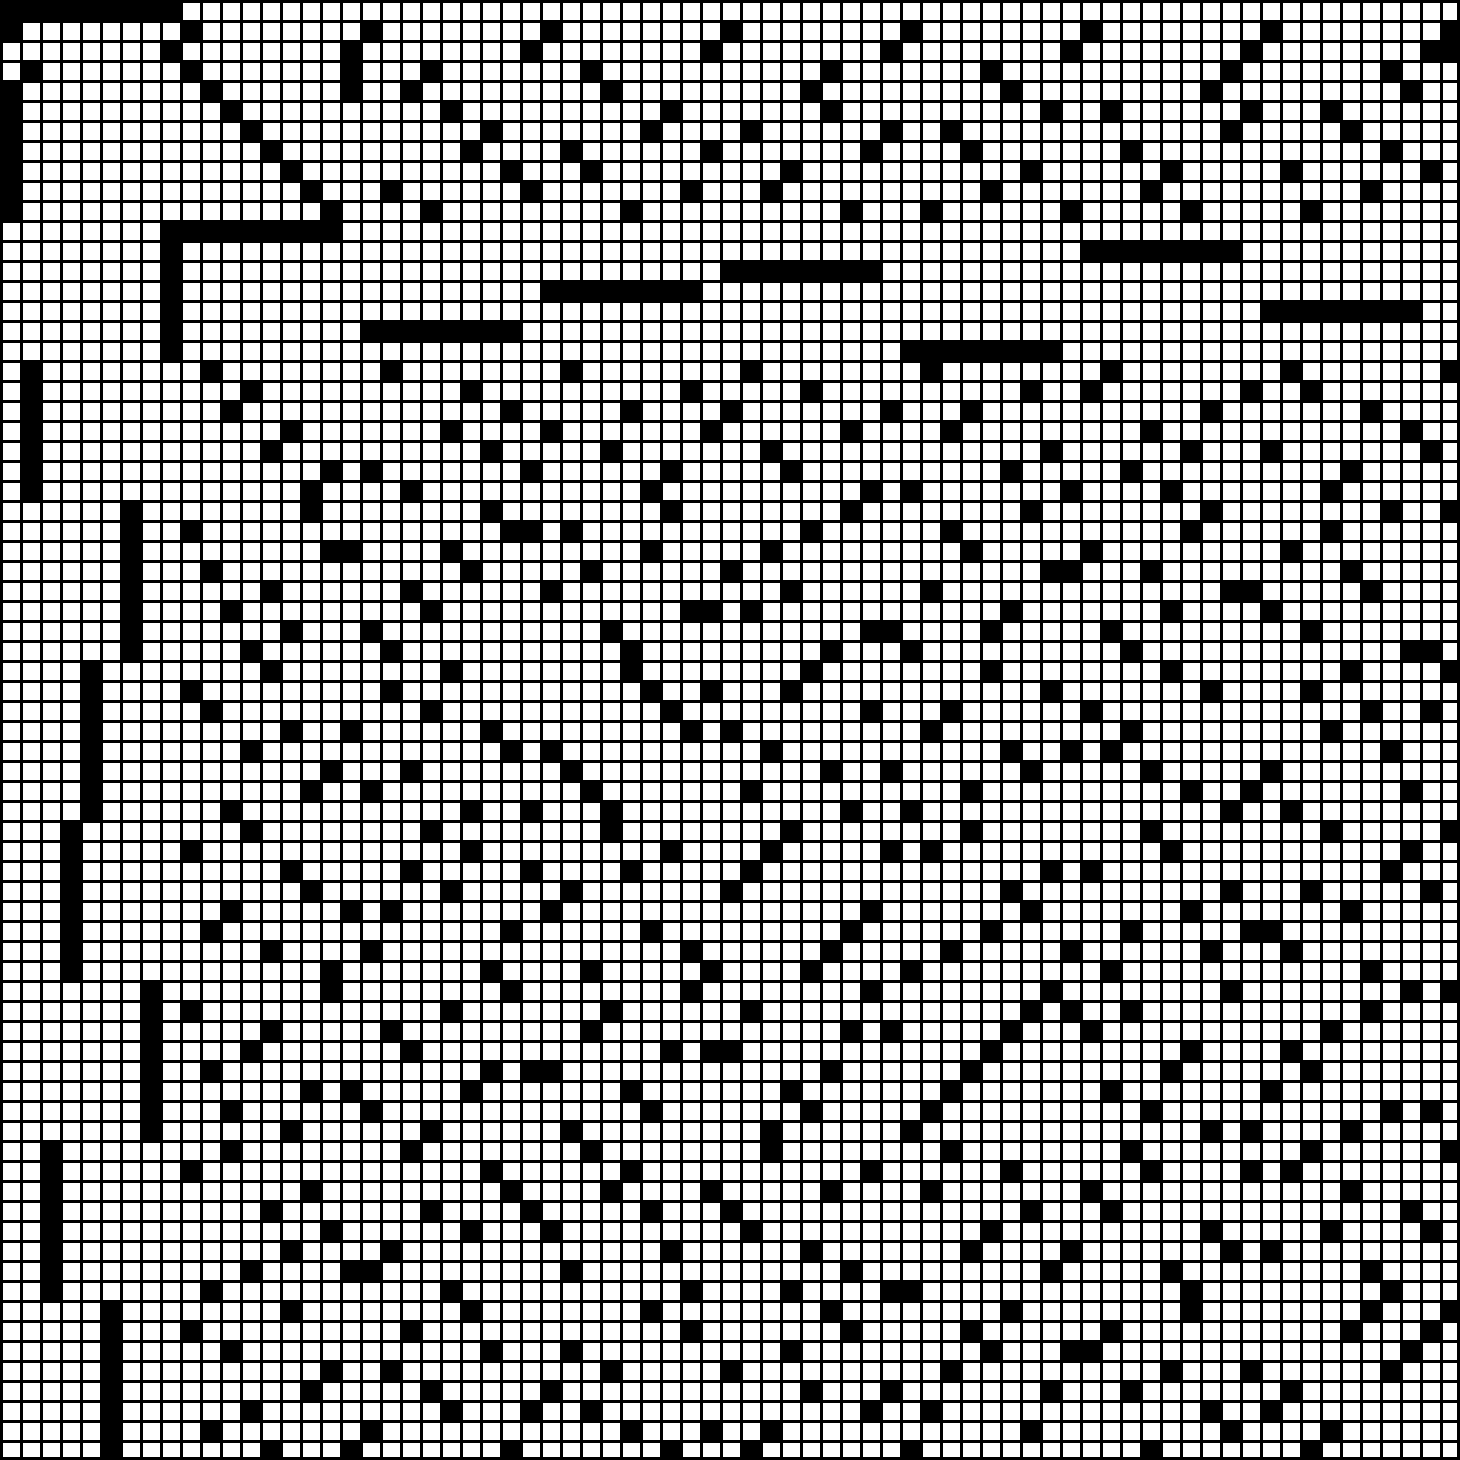
\includegraphics[width=13cm]{GRAPHICS/PG/PG_n2_q8_incidence_matrix_draw}
$$
\caption{\label{fig:incidence:matrix:PG:2:8}Incidence matrix of $\PG(2,8)$ in Orbiter ordering}
\end{figure}
The rows and columns correspond to points and lines, respectively. 
The Orbiter indexing of points and lines determines the ordering of rows and columns.



\bigskip


The projective spaces $\PG(2,q)$ deserve special attention. 
They are examples of a more general structure called projective planes. 
The $\PG(2,F)$, $F$ a field, are distinguished 
in the class of projective planes by the fact that the theorem of Desargues 
always holds.
They are called the desarguesian projective planes.
For other projective planes, see Section~\ref{sec:translation:planes}. 


\bigskip

The points in the dearguesian projective plane $\PG(2,q)$ 
have the coordinates $P(x,y,z),$ with $x,y,z\in \bbF_q.$ 
We can distingish one line, for instance $z=0$, and call it the line at infinity. 
The points not on that line form an affine plane $\AG(2,q).$

\bigskip



The command 
{\tt
\input GRAPHICS/THE_MAKEFILE/EXTRACTS/PG_2_16.tex
}
produces the drawing of $\PG(2,16)$ shown in Figure~\ref{fig:PG:2:16}.
\begin{figure}
$$
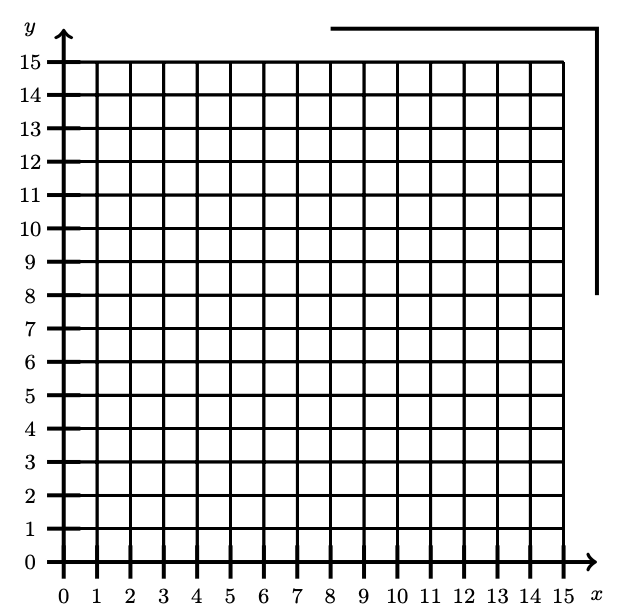
\includegraphics[width=9cm]{GRAPHICS/PG/PG_2_16}
$$
\caption{\label{fig:PG:2:16}The plane $\PG(2,16)$}
\end{figure}
The \verb'-nodes_empty' command is used to suppress the drawing of the nodes.
The \verb'-xin 20000' and \verb'-yin 20000' options double the input coordinate system 
(recall from Table~\ref{tab:draw:options} that the default values are 10000), 
which has the effect that the text appears smaller relative to the 
grid.


\bigskip


Projective spaces has a special property.  They admit a cyclic group action on points and hyperplanes. 
Such a group is often called a Singer cycle. 
It is generated from a projectivity defined by the companion matrix of an irreducible polynomial. 
Let us look at an example. 
The following command creates a Singer cycle of $\PG(2,4)$
{\tt
\input GRAPHICS/THE_MAKEFILE/EXTRACTS/PG_2_4_with_decomposition.tex
}
The ouput is shown below:
\begin{mdframed}[style=MyFrame]
\input GRAPHICS/LATEX/report_PG_2_4_singer.tex
\end{mdframed}

\bigskip

The command produces a csv file containing the cyclic incidence matrix, which can be 
visualized using the follwing command:
{\tt
\input GRAPHICS/THE_MAKEFILE/EXTRACTS/PG_2_4_incma_cyclic.tex
}
The cyclic incidence matrix is shown in Figure~\ref{fig:PG:2:4:cyclic}.
\begin{figure}
$$
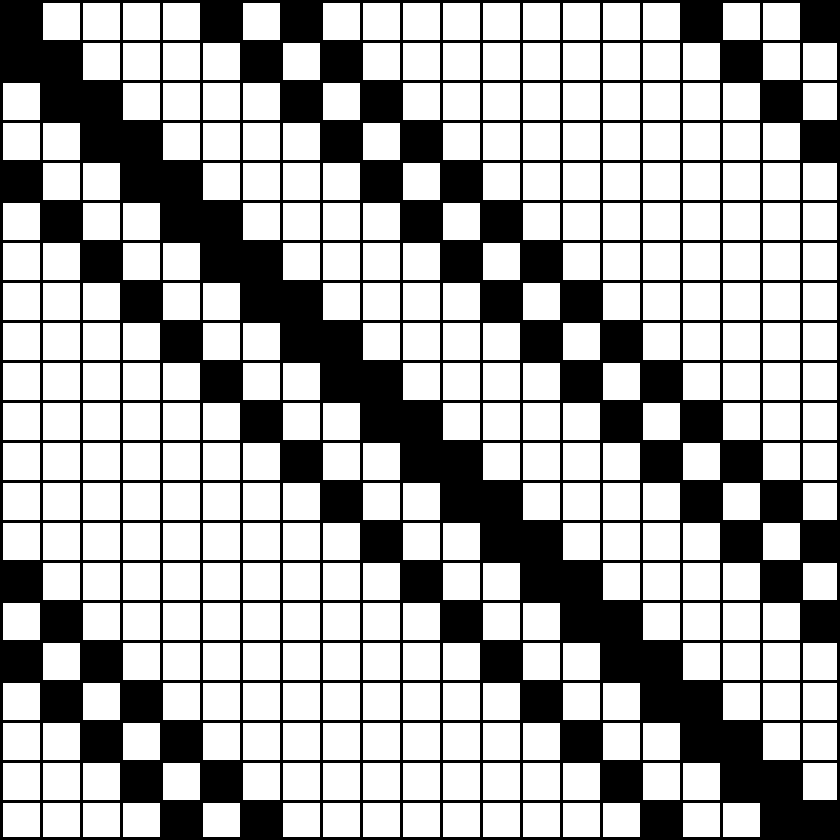
\includegraphics[width=9cm]{GRAPHICS/PG/PG_2_4_singer_incma_cyclic_draw}
$$
\caption{\label{fig:PG:2:4:cyclic}Cyclic incidence matrix of  $\PG(2,4)$}
\end{figure}

\bigskip



If the number of points is not a prime, the group acts imprimitively.
By considering various subgroups, tactical decompositions are created.
For instance, for $\PG(2,4),$ with 21 points, 
we can consider a subgroup the Singer cycle of order 3, which induces a 
partition with 7 classes of size 3 on both points and lines:
{\tt
\input GRAPHICS/THE_MAKEFILE/EXTRACTS/PG_2_4_incma_singer_sub_3.tex
}
The tactical decomposition of the incidence matrix is 
shown in Figure~\ref{fig:PG:2:4:cyclic:subgroup3}.
\begin{figure}
$$
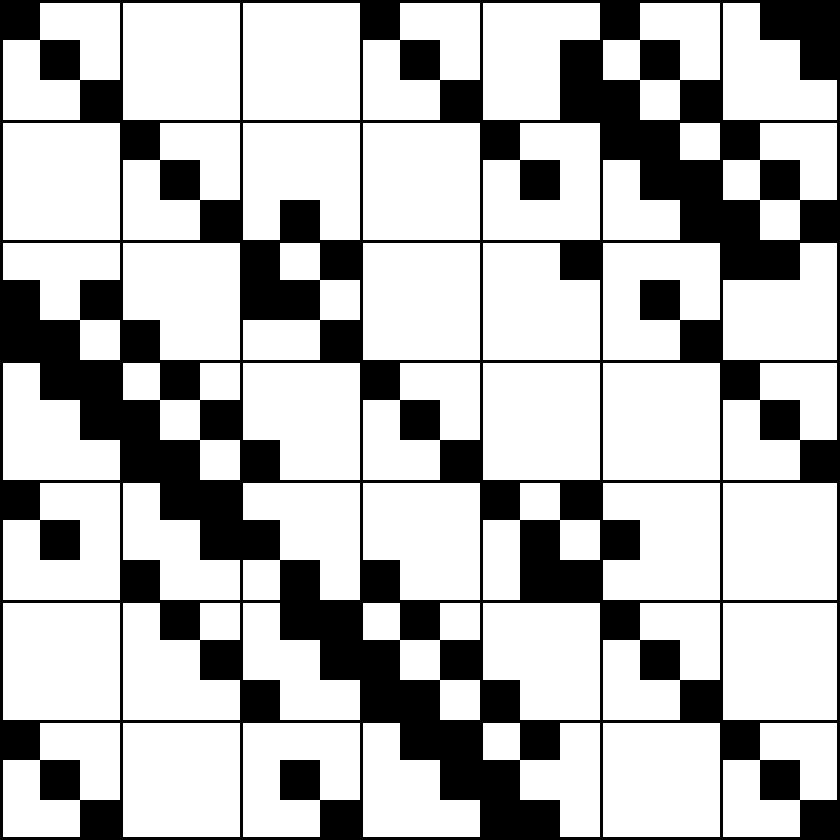
\includegraphics[width=9cm]{GRAPHICS/PG/PG_2_4_singer_incma_subgroup_index_3_draw}
$$
\caption{\label{fig:PG:2:4:cyclic:subgroup3}Tactical decomposition 
of the incidence matrix of  $\PG(2,4)$}
\end{figure}


\bigskip


Let $V$ be a finite dimensional vector space and 
let ${\mathfrak Gr}_k(V)$ be the Grassmannian of $k$-dimensional subspaces 
of $V.$ 
If $\dim(V) = n,$ the notation ${\mathfrak Gr}_{n,k}$ is used for ${\frak Gr}_k(V).$ 
If $V = \bbF_q^n,$ the notation ${\mathfrak Gr}_{n,k,q}$ is used for ${\frak Gr}_k(V).$ 
The order of the set ${\frak Gr}_{n,k,q}$ can be computed as
$$
\left[
n \atop k
\right]_q = 
\prod_{i=0}^{k-1}\frac{q^{n-i}-1}{q^{k-i}-1},
$$
using the $q$-binomial coefficient.

\bigskip

Orbiter has an enumerator for the Grassmannian. 
The purpose of this enumerator is to establish a bijection 
between the Grassmannian and the integers in the interval 
$
[0,N-1],
$ 
where $N = \left[
n \atop k
\right]_q.$
In order to do so, Orbiter picks a basis for each subspace. 
By writing the elements of the basis in the rows of a matrix, a $k\times n$ matrix is obtained. 
In order to make the matrix unique, we assume it to be in RREF. 
In coding theory, such a matrix is called a generator matrix.

\bigskip


The Orbiter cheat sheets for $\PG(n,q)$ (see Section~\ref{sec:FPG}) 
contain lists of all Grassmannians, provided they are not too big.
It is also possible to create cheat sheets specifically for one Grassmannian.
For instance, the command
{\tt
\input GRAPHICS/THE_MAKEFILE/EXTRACTS/GR_3_2_2.tex
}
produces a list of 2-dimensional 
subspaces of $\bbF_2^3,$ i.e. the lines of $\PG(2,2):$
\begin{mdframed}[style=MyFrame]
\input GRAPHICS/LATEX/report_Gr_3_2_2.tex
\end{mdframed}

\bigskip

The following command illustrates how to rank lines.
In the example, we consider lines in $\PG(3,3).$
The lines are given as vectors of length $8.$ Three lines are given in \verb'v1' 
and three lines are given in \verb'v2'.
{\tt
\input GRAPHICS/THE_MAKEFILE/EXTRACTS/PG_3_3_rank_lines.tex
}


\bigskip

In the next example, we unrank six lines in $\PG(3,5).$
{\tt
\input GRAPHICS/THE_MAKEFILE/EXTRACTS/PG_3_5_unrank_lines.tex
}

\bigskip


The following command produces a list of planes through a line. 
In the example, the line is $0$. The projective space is $\PG(3,8)$
{\tt
\input GRAPHICS/THE_MAKEFILE/EXTRACTS/planes_in_pencil.tex
}



\bigskip




A set of points $V$ in $\PG(n,q)$ is algebraic if there is a set 
of homogeneous polynomials $p_1,\ldots,p_r$
whose roots over $\bbF_q$ are the given set. 
In this case, we write $V = \bv(p_1,\ldots,p_r).$ 
The set $V$ is often called the variety of $p_1,\ldots,p_r.$

\bigskip

Conversely, given a set of points $V$ in $\PG(n,q),$ 
the ideal $I(V)$ is the set of homogeneous polynomials 
in $\bbF_q[X_0,\ldots,X_n]$ which vanish on all of $V.$
This set is an ideal in the polynomial ring. 
In $\PG(n,q),$ every set is algebraic 
of degree at most $(n+1)(q-1)$~\cite{GlynnHirschfeld95}. 
The associated polynomial is unique and known as 
the algebraic normal form of the set.


\bigskip


In order to work with algebraic sets, multivariate polynomial rings are required. 
For details, see Section~\ref{sec:ring:theory:multivariate}.

\bigskip


Suppose we are interested in $\bbF_{11}$-rational points of 
the elliptic curve $y^2= x^3+x+3.$
We write $x^3+3-y^2+x = 0.$ 
Homogenizing yields $X^3+3Z^3-Y^2Z+XZ = 0.$
Using $X_0,X_1,X_2$ instead of $X,Y,Z$ yields
$$
X_0^3+3X_2^3 + 10X_1^2X_2  + X_0X_2^2 = 0.
$$
Using the indexing of monomials from 
Table~\ref{tab:PG2monomials}, 
we record the coefficient vector of the equation as sequence
$$
(1,0,3,0,0,0,10,1,0,0).
$$
The Orbiter command
{\tt
\input GRAPHICS/THE_MAKEFILE/EXTRACTS/EC_11_EQUATION.tex
}
{\tt
\input GRAPHICS/THE_MAKEFILE/EXTRACTS/EC_11.txt.tex
}
creates the algebraic set associated to the cubic curve $y^2=x^3+x+3$ in $\PG(2,11).$ 
It turns out that there are exactly $18$ 
points over $\bbF_{11}$ (cf. Figure~\ref{fig:EC_11_1_3}). 
\begin{figure}
$$
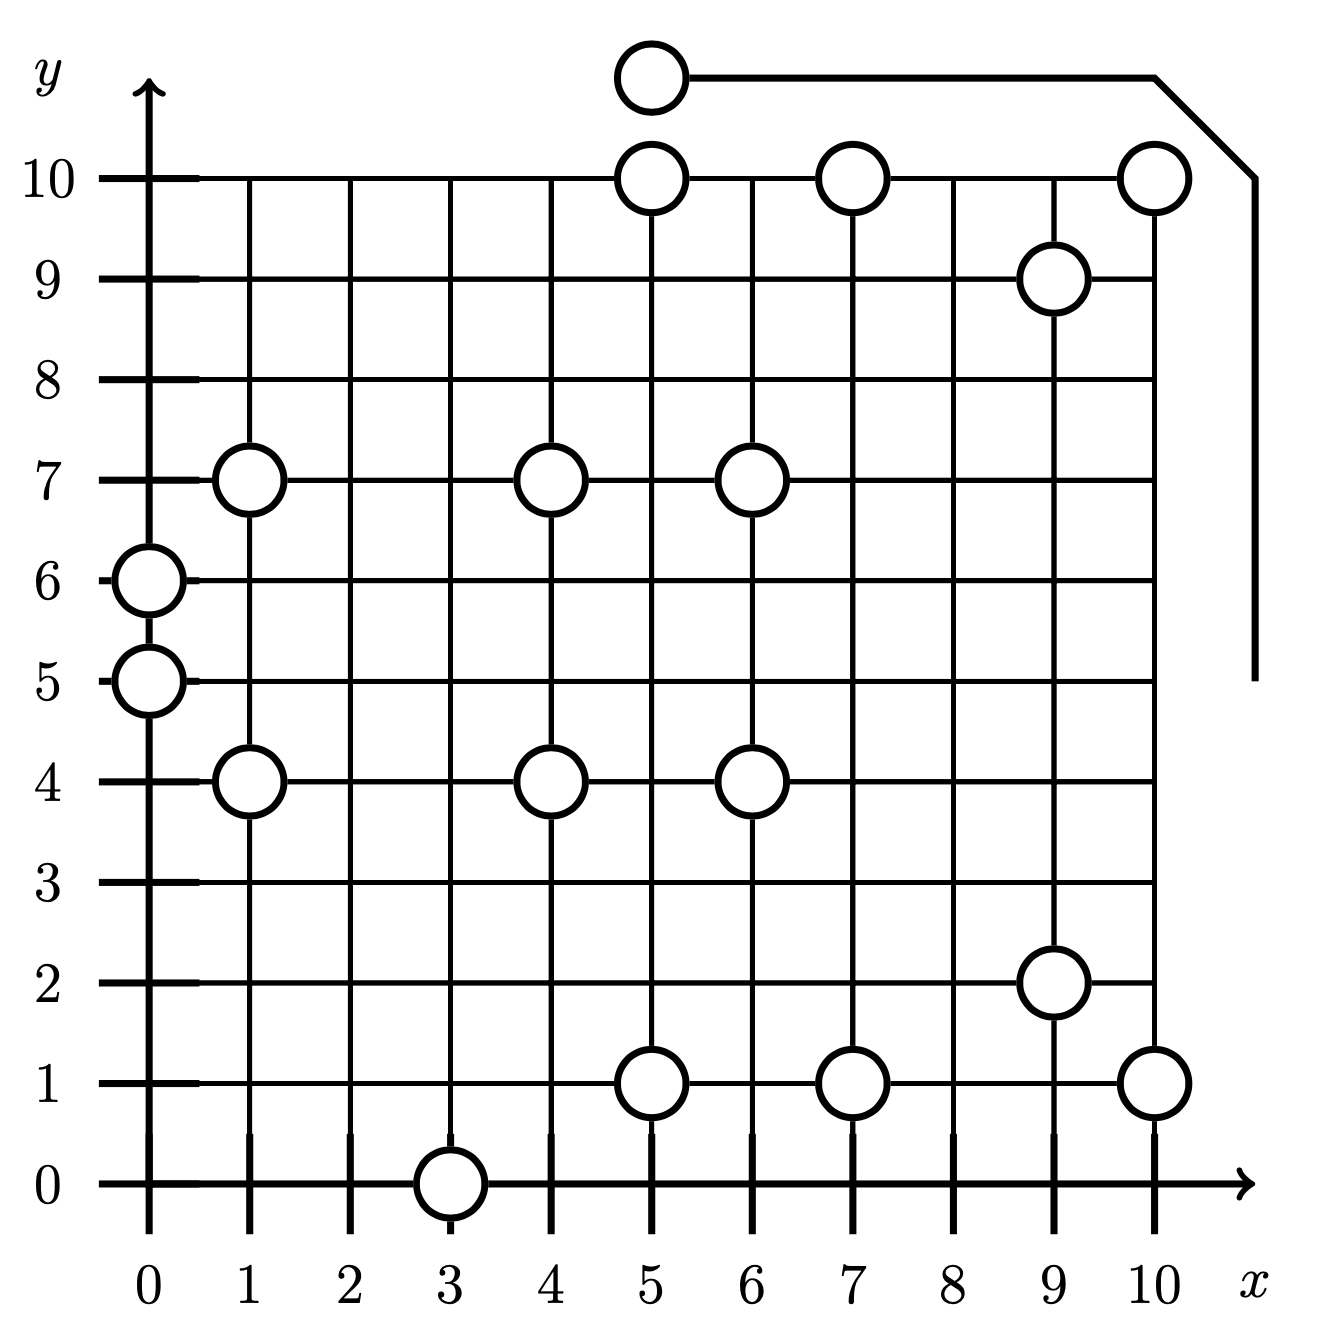
\includegraphics[width=8cm]{CODE/FILES/EC_11_1_3/EC_11_1_3}
$$
\caption{\label{fig:EC_11_1_3}Elliptic curve $y^2\equiv x^3+x+3$ mod $11$}
\end{figure}
Suppose we want to create the Hirschfeld surface with equation
$$
X_0^2X_3 + X_1^2X_2 + X_1X_2^2 + X_0X_3^2=0.
$$  
Based on the partition ordering of Figure~\ref{tab:PG3monomials}, 
the equation is coded as coefficient vector
$$
(0,0,0,0,0,0,1,0,1,0, 0,1,0,1,0,0,0,0,0,0).
$$
The following command can be used to create the variety over $\bbF_4$:
{\tt
\input GRAPHICS/THE_MAKEFILE/EXTRACTS/HIRSCHFELD_SURFACE_EQUATION.tex
}
{\tt
\input GRAPHICS/THE_MAKEFILE/EXTRACTS/Hirschfeld_surface_q4.txt.tex
}
A file called \verb'Hirschfeld_surface_q4.txt' is created. 
The file contains the Orbiter 
ranks of the $45$ points on the surface.


\bigskip

Orbiter can work with the Grassmannian over a finite field. 
In particular, Orbiter offers indexing for subspaces.
For the special case of the Grassmannian ${\mathfrak Gr}_{4,2}(V)$, 
Pl\"ucker coordinates can be used to identify 
${\mathfrak Gr}_{4,2}(V)$ with the $Q^+(5,q)$ (Klein) quadric.
Here is an example. The command 
{\tt
\input GRAPHICS/THE_MAKEFILE/EXTRACTS/GR_4_2_2.tex
}
creates the elements of ${\mathfrak Gr}_{4,2,2}$ 
and lists them together with their Pl\"ucker coordinates.
The following list is produced (output shortened): 
\begin{mdframed}[style=MyFrame]
\input GRAPHICS/LATEX/report_Gr_4_2_2.tex
\end{mdframed}
The Pl\"ucker coordinates satisfy
$$
p_{12}p_{34} - p_{13}p_{24}+p_{14}p_{23}=0
$$
and hence belong to the Klein quadric $Q^+(5,q)$.
Orthogonal spaces and quadrics will 
be discussed in Section~\ref{sec:orthogonal}.

\bigskip


The Orbiter labeling of points of 
the $Q^+(5,q)$ quadric (see Section~\ref{sec:orthogonal}) 
can then be used to enumerate the lines of $\PG(3,q)$ in a second, different way.
In the example of $\PG(3,2),$ 
this yields the following list (output shortened):
\begin{mdframed}[style=MyFrame]
\input GRAPHICS/LATEX/report_Op_5_2.tex
\end{mdframed}


Orbiter can create and work with orthogonal spaces and their groups.
An orthogonal space is created by a quadratic form. 
We assume that the form is nondegenerate.
There are three types of nondegenerate quadratic forms in $\PG(n,q).$ 
Two when $n$ is odd (hyperbolic and elliptic) and one if $n$ is even (parabolic).
Basic information about these quadrics and their representative quadratic forms in Orbiter 
is given in Table~\ref{tab:quadrics}.
Here, $p(X,Y)=c_1X^2+ c_2XY+c_3Y^2 \in \bbF_q[X,Y]$ is irreducible over $\bbF_q.$ 
\begin{table}
	\begin{center}
		{\renewcommand{\arraystretch}{1.5}
	\begin{tabular}{|c|c|c|c|}
		\hline
		Type & Quadratic Form & \# Points  \\
		\hline
		\hline
		\begin{tabular}{c}
		$Q^+(n,q)$\\
		Hyperbolic ($n$ is odd)\\
		\end{tabular}	  & $\displaystyle \sum_{i=0}^{\frac{n-1}{2} - 1} X_{2i}X_{2i+1}$ &  
		$\displaystyle \frac{(q^{(n+1)/2}-1)(q^{(n-1)/2}+1)}{q-1}$ \\
		\hline
		\begin{tabular}{c}
		$Q^-(n,q)$\\
		Elliptic ($n$ is odd) \\
		\end{tabular}
		& $\displaystyle p(X_{n-1}, X_{n}) + \sum_{i=0}^{\frac{n-1}{2} - 1} X_{2i}X_{2i+1}$  &  
		$\displaystyle \frac{(q^{(n+1)/2}+1)(q^{(n-1)/2}-1)}{q-1}$  \\
		\hline
		\begin{tabular}{c}
		$Q(n,q)$\\
		Parabolic ($n$ is even)  \\
		\end{tabular}
		& $\displaystyle X_0^2 + \sum_{i=0}^{\frac{n}{2} - 1} X_{2i+1}X_{2i+2}$  &  $\displaystyle \frac{q^n-1}{q-1}$ \\
		\hline
		\end{tabular}
		}
	\end{center}
	\caption{\label{tab:quadrics}Nondegenerate Quadrics in $\PG(n,q)$ and the canonical form adopted in Orbiter}
	\end{table}
To create an orthogonal space, the 
$$
\verb'-orthogonal_space' \; \epsilon \; d \; q \; \verb'-end'
$$
command can be used. 
Here, $d = n + 1$, $q$ is the order of the finite field, and  
$$
\epsilon = 
\left\{
\begin{array}{cccc}
1 & \mbox{hyperbolic type} & Q^+(d-1,q), &  d \; \mbox{even} \\
0 & \mbox{elliptic type} & Q(d-1,q), & d \; \mbox{odd} \\
-1 & \mbox{hyperbolic type} & Q^-(d-1,q),& d \; \mbox{even} \\
\end{array}
\right.
$$
In Table~\ref{tab:orthogonal}, Orbiter command options for creating orthogonal spaces are shown.
\begin{table}
\begin{center}
\begin{tabular}{|p{4cm}|c|p{8cm}|}
\hline
Command & Arguments & Purpose \\
\hline
\hline
\verb'-label_txt' & L & Set the ascii-label of the space. The label is used for things like file names etc. 
A default label will be used if this option is not given. \\
\hline
\verb'-label_tex' & L & Set the tex-label of the space. The label is used within latex reports. 
A default label will be used if this option is not given. \\
\hline
\verb'-without_group' &  & Do not create the orthogonal group. \\
\hline
\end{tabular}
\end{center}
\caption{\label{tab:orthogonal}Command options to create an orthogonal space}
\end{table}

\bigskip

For instance, the following command creates $Q(3,2)$ together with its group $PGO^+(4,2)$:
{\tt
\input GRAPHICS/THE_MAKEFILE/EXTRACTS/Op_4_2.tex
}

\bigskip

The next command creates $Q(4,2)$ together with its group $PGO(5,2)$. 
There are 15 points and 15 lines.
The geometry is a configuration $15_3$ which is also 
known as the Cremona-Richmond configuration.
{\tt
\input GRAPHICS/THE_MAKEFILE/EXTRACTS/O_5_2_incidence_matrix.csv.tex
}
The command also 
creates a bitmap drawing of the incidence matrix between points and lines of $Q(4,2).$
The incidence matrix is shown in Figure~\ref{fig:O:5:2:incidence}.
The Orbiter indexing for points and lines of quadrics is used to order the rows and columns.
\begin{figure}
$$
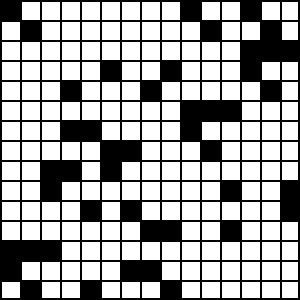
\includegraphics[width=7cm]{GRAPHICS/PGO_5_2/O_5_2_incidence_matrix_draw}
$$
\caption{\label{fig:O:5:2:incidence}Incidence matrix of $Q(4,2)$}
\end{figure}





\bigskip



By default, the orthogonal space is created together with the orthogonal group 
${\rm P}{\Gamma}{\rm O}(n+1,q)$. 
When $q$ is prime, the group ${\rm P}{\rm G}{\rm O}(n+1,q)$ 
is created instead (the groups are isomorphic in this case, 
and ${\rm P}{\rm G}{\rm O}(n+1,q)$ is a bit more efficient). 
For large orthogonal spaces, creating the group is expensive in terms of time and memory. 
The a command \verb'-without_group' can be used to prevent the group from being created. 
For instance
$$
\verb'-define O -orthogonal_space 1 6 2 -end'
$$
creates an object $O$ of type $Q^+(5,2).$
In Table~\ref{tab:orthogonal:activities}, Orbiter activities for orthogonal spaces are shown.
\begin{table}
\begin{center}
\begin{tabular}{|p{4cm}|c|p{8cm}|}
\hline
Command & Arguments & Purpose \\
\hline
\hline
\verb'-create_BLT_set' & descr & Creates a BLT-set of $Q(4,q).$ See Section~\ref{sec:BLT:sets}. \\
\hline
%\verb'-BLT_set_starter' & $s$ & Classify partial BLT-sets of size $\le s$.  \\
%\hline
%\verb'-BLT_set_graphs' & $s$ $r$ $m$ & Create the lifting graphs for all partial BLT-sets of size $s$. Process only the cases whose number is congruent to $r$ mod $m$ ($0 \le r < m$).  \\
%\hline
%\verb'-fname_base_out' & fname & Set file name for output files. \\
%\hline
\verb'-cheat_sheet_' \verb'orthogonal' &  & Create a cheat sheet.  \\
\hline
\verb'-print_points' & $v$ & Print the points whose ranks are given in the vector $v$. \\
\hline
\verb'-print_lines' & $v$ & Print the lines whose ranks are given in the vector $v$. \\
\hline
\verb'-unrank_line_' \verb'through_two_points' & $p1$ $p2$ & 
Determine the rank of the line through the points whose ranks are $p1$ and $p2$. \\
\hline
\verb'-lines_on_point' & $p$ &  Create the ranks of all lines through the point whose rank is $p$. \\
\hline
\verb'-perp'  & $L$ & 
Determine the common perp of a set of points. The point ranks are given in the list $L$.  \\
\hline
\verb'-export_point_' \verb'line_incidence_' \verb'matrix'  &  & 
Create a csv file with the point line incidence matrix of the space.  \\
\hline
\verb'-intersect_with_' \verb'subspace'  & $M$ & 
Find the points in the intersection of the quadric 
with the subspace whose generating matrix has label $M$. \\
\hline
\end{tabular}
\end{center}
\caption{\label{tab:orthogonal:activities}Activities related to orthogonal spaces}
\end{table}

\bigskip


The command 
{\tt
\input GRAPHICS/THE_MAKEFILE/EXTRACTS/Op_6_2.tex
}
produces a cheat sheet for the quadric $Q^+(5,2)$. 
This is the Klein quadric from Section~\ref{sec:klein}.
Orbiter produces the following output. 
At the top is the tactical decomposition of the incidence matrix between points and lines 
with respect to a hyperbolic pair. 
After that, the points and lines are listed (output shortened):
\begin{mdframed}[style=MyFrame]
\input GRAPHICS/LATEX/report_Op_6_2.tex
\end{mdframed}
Orbiter has enumerators for points and lines in orthogonal spaces. 
For small spaces, 
the cheat sheet lists points and lines in the Orbiter ordering.
Creating the groups can be expensive.
For large spaces, it may be necessary 
to disable the group using the \verb'-without_group' option.
The command 
{\tt
\input GRAPHICS/THE_MAKEFILE/EXTRACTS/Op_6_64_line_rank.tex
}
computes the Orbiter rank of the line through 
the points with rank $15447347$ and $15225451$, respectively.
The rank of the line is $16767254$.
These ranks refer to the orthogonal geometry. 
They are different from the ranks of points and lines in projective spaces.

\bigskip

It is possible to create reports for orthogonal spaces without group. 
In this case, the group information will be skipped. 
For instance, the following command creates a report for $Q(5,64)$:
{\tt
\input GRAPHICS/THE_MAKEFILE/EXTRACTS/Op_6_64_report.tex
}
The report does not show information about the group. 
However, it still contains the tactical decomposition with respect to a hyperbolic pair. 
The printing of points is restricted to small spaces only.

\bigskip

\begin{mdframed}[style=MyFrame]
\input GRAPHICS/LATEX/report_Op_6_64.tex
\end{mdframed}


\bigskip

To study BLT-sets in $Q(4,q)$, see Section~\ref{sec:BLT:sets}.

\bigskip


According to Table~\ref{tab:quadrics}, Orbiter uses the equation 
$$
X_0X_1+
X_2X_3+
X_4X_5 = 0
$$
to define the Klein quadric.
An elliptic quadric is an ovoid of the Klein quadric that is 
obtained by intersecting the quadric with a suitable solid.
In $\PG(5,5),$
the subspace generated by the rows of the matrix
$$
\left[
\begin{array}{cccccc}
1&3&0&0&0&0 \\
0&0&1&0&0&0 \\
0&0&0&1&0&0 \\
0&0&0&0&1&1 \\
\end{array}
\right]
$$
is such a subspace.
The ordering of columns corresponds to the natural 
ordering of the variables as $X_0, X_1, X_2, X_3, X_4, X_5.$
The following command produces a list 
of points of an elliptic quadric ovoid in $Q^+(5,5).$
{\tt
\input GRAPHICS/THE_MAKEFILE/EXTRACTS/elliptic_quadric_subspace.tex
}
The elliptic quadric has 26 points.


\bigskip


The coding of points and line in orthogonal spaces 
is different from the coding of points in projective spaces. 
We will create and print a set called BLT set (after~\cite{BaderLunardonThas90}). 
This is a set of $q+1$ points on the $Q(4,q)$ quadric satisfying a special geometric property. 
According to Table~\ref{tab:quadrics}, Orbiter uses the equation 
$$
X_0^2+
X_1X_2+
X_3X_4 = 0
$$
to define the $Q(4,q)$ quadric.
The following example creates the BLT-set with Orbiter catalogue number \#1 in $Q(4,7)$:
{\tt
\input GRAPHICS/THE_MAKEFILE/EXTRACTS/BLT_database_7_1.tex
}
The set is stored in a file.
The next command reads the file and prints the elements of the set:
{\tt
\input GRAPHICS/THE_MAKEFILE/EXTRACTS/BLT_database_7_1_print.tex
}
The command produces the following list of points, 
comprising the second BLT-set over $\bbF_7$.
\begin{mdframed}[style=MyFrame]
\input GRAPHICS/LATEX/report_BLT_q7.tex
\end{mdframed}
More on BLT-sets can be found in Section~\ref{sec:BLT:sets}.

\bigskip

The next command prints points and lines of the $W(2),$ also known as the Doily.
It is an example of a generalized quadrangle.
{\tt
\input GRAPHICS/THE_MAKEFILE/EXTRACTS/Doily_W_2.tex
}

Orbiter has enumerators for points of the hermitian variety ${\rm H}(k,Q)$.
Here, $Q$ is a square, and so $q = \sqrt{Q}$ is an integer. The equation of the variety is 
$$
\sum_{i=0}^k X_i^{q+1} = 0.
$$
The command 
{\tt
\input GRAPHICS/THE_MAKEFILE/EXTRACTS/H_2_4.tex
}
produces a cheat sheet for the variety $H(2,4)$:\\
\begin{mdframed}[style=MyFrame]
\input GRAPHICS/LATEX/report_Hermitian_2_4.tex
\end{mdframed}

\bigskip

The command 
{\tt
\input GRAPHICS/THE_MAKEFILE/EXTRACTS/H_3_4.tex
}
produces a cheat sheet for the variety $H(3,4)$.


\bigskip


\begin{mdframed}[style=MyFrame]
\input GRAPHICS/LATEX/report_Hermitian_3_4.tex
\end{mdframed}

\bigskip

Coincidentally, this Hermitian variety is the Hirschfeld cubic surface over $\bbF_4.$


The Orbiter commands associated with projective space objects are summarized in 
Tables~\ref{tab:projective:space:activities:1}-\ref{tab:projective:space:activities:4}.
\begin{table}
	\begin{center}
	\begin{tabular}{|p{4cm}|p{3cm}|p{7cm}|}
		\hline
		Command & Arguments & Purpose \\
		\hline
		\hline
		\verb'-export_point_' \verb'line_incidence_' \verb'matrix' &  &  Create a csv file of the point line incidence matrix. \\
		\hline
		\verb'-table_of_' \verb'cubic_surfaces_' \verb'compute_properties' &  fname $q_0$ col-offset  &   See Section~\ref{sec:cubicsurfaces:Dickson}. \\
		\hline
		\verb'-cubic_surface_' \verb'properties_analyze' & fname $q_0$    &  See Section~\ref{sec:cubicsurfaces:Dickson}. \\
		\hline
		\verb'-canonical_form_' \verb'of_code' &  label $m$ $n$ matrix  &  Compute the automorphism group of a linear code using Nauty. See Section~\ref{sec:coding}.  \\
		\hline
		\verb'-map' & label parameters   &  evaluate a formula using the given parameters \\
		\hline
		\verb'-analyze_' \verb'del_Pezzo_surface' &  label parameters  &   \\
		\hline
		\verb'-cheat_sheet_for_' \verb'decomposition_by_' \verb'element_PG' & power elt fname   & 
		Analyzes the orbit structure of the cyclic group 
		generated by the given element in the action on $\PG(n,q).$ \\
		\hline
		\verb'-cheat_sheet_for_' \verb'decomposition_by_' \verb'subgroup' & label descr   & 
		Analyzes the orbit structure of the subgroup $H$ in the action on $\PG(n,q).$ 
		The subgroup must be a linear group, 
		and the description of $H$ must come from the commands from Section~\ref{sec:lineargroups}. \\
		\hline
		%\verb'-define_surface' &  label descr  &  To create a cubic surface and add it to the symbol table under the given label. 
		%See Section~\ref{sec:cubicsurfaces:creation}. \\
		%\hline
		\verb'-table_of_' \verb'quartic_curves' &    &  Export the classification of quartic curves to a csv file. \\
		\hline
		\verb'-table_of_' \verb'cubic_surfaces' &    &  Export the classification of cubic surfaces to a csv file. \\
		\hline
		%\verb'-define_' \verb'quartic_curve' &  label descr  &  To create a quartic curve and add it to the symbol table under the given label. 
		%See Section~\ref{sec:cubic:surfaces:quartic:curves}. \\
		%\hline
		\verb'-classify_surfaces_' \verb'with_double_sixes' & label control   & Classify cubic surfaces using the approach of double sixes. 
		See Section~\ref{sec:cubicsurfaces:classification}.  \\
		\hline
		\end{tabular}
	\end{center}
	\caption{\label{tab:projective:space:activities:1}Projective Space Activities (Part 1)}
\end{table}
\begin{table}
	\begin{center}
	\begin{tabular}{|p{4cm}|p{3cm}|p{7cm}|}
		\hline
		Command & Arguments & Purpose \\
		\hline
		\hline
		\verb'-classify_surfaces_' \verb'through_arcs_' \verb'and_two_lines' &    &  
		Classify cubic surfaces using the approach of six-arcs and two skew lines. 
		See Section~\ref{sec:cubicsurfaces:classification}.  \\
		\hline
		\verb'-classify_surfaces_' \verb'through_arcs_' \verb'and_trihedral_pairs' &    & See Section~\ref{sec:cubicsurfaces:classification}.  \\
		\hline
		\verb'-test_nb_Eckardt_' \verb'points' &  $e$  & Restrict to $e$ Eckardt points. See Section~\ref{sec:cubicsurfaces:classification}. To be used in conjunction with \verb'-classify_surfaces_' \verb'through_arcs_' \verb'and_trihedral_pairs'.  \\
		\hline
		%\verb'-create_surface' &  description  & Create a cubic surface  \\
		%\hline
		\verb'-sweep' & fname   &   \\
		\hline
		\verb'-sweep_4' &  fname surface-descr &   \\
		\hline
		\verb'-sweep_4_27' &  fname surface-descr  &   \\
		\hline
		\verb'-six_arcs_' \verb'not_on_conic' &    & Classify six-arcs not on a conic in a plane.   \\
		\hline
		\verb'-filter_by_nb_' \verb'Eckardt_points' & $e$   &  Filter for the number of Eckardt points to be equal to $e$. Used in conjunction with \verb'-six_arcs_' \verb'not_on_conic'. \\
		\hline
		%\verb'-surface_quartic' &    &   \\
		%\hline
		%\verb'-surface_clebsch' &    &   \\
		%\hline
		%\verb'-surface_codes' &    &   \\
		%\hline
		\verb'-trihedra1_control' &   poset-control &  For \verb'-classify_surfaces_' \verb'through_arcs_' \verb'and_trihedral_pairs' \\
		\hline
		\verb'-trihedra2_control' & poset-control   &  For \verb'-classify_surfaces_' \verb'through_arcs_' \verb'and_trihedral_pairs' \\
		\hline
		\verb'-control_six_arcs' &  poset-control  &  For \verb'-classify_surfaces_' \verb'through_arcs_' \verb'and_trihedral_pairs' \\
		\hline
		%\verb'-make_gilbert_' \verb'varshamov_code' & $n$ $d$    & See Section~\ref{sec:Bounds}.  \\
		%\hline
		\end{tabular}
	\end{center}
	\caption{\label{tab:projective:space:activities:2}Projective Space Activities (Part 2)}
\end{table}
\begin{table}
	\begin{center}
	\begin{tabular}{|p{4cm}|p{3cm}|p{7cm}|}
		\hline
		Command & Arguments & Purpose \\
		\hline
		\hline
		%\verb'-spread_classify' &  $k$ control  &  OUTDATED. See Section~\ref{sec:spreads}. \\
		%\hline
		\verb'-classify_' \verb'semifields' & descr   &   \\
		\hline
		\verb'-cheat_sheet' &    & Produce a cheat sheet for $\PG(n,q)$  \\
		\hline
		\verb'-classify_quartic_' \verb'curves_nauty' & fname-mask $N$  fname & Classify quartic curves using Nauty.  \\
		\hline
		\verb'-classify_quartic_' \verb'curves_with_' \verb'substructure' & fname-mask $N$  $k$ $d$ fname & Classify quartic curves using substructure algorithm.  \\
		\hline
		\verb'-set_stabilizer' & $k$ fname-mask $N$  col-label fname-out & Compute canonical form of sets using the substructure algorithm. \\
		\hline
		\verb'-conic_type' & $t$ set & Compute the conic type of the given set (given by its label). Record intersections of size $\ge t$ only.   \\
		\hline
		%\verb'-lift_skew_hexagon' & text & Lift a skew-hexagon. \\
		%\hline
		%\verb'-lift_skew_hexagon_' \verb'with_polarity' & polarity & Lift a skew-hexagon with a given polarity. \\
		%\hline
		\verb'-arc_with_given_' \verb'set_as_s_lines_' \verb'after_dualizing' & $sz$ $d$ $d_{\min}$ $s$  & 
		Finds arcs with the given set as $s$-lines. \\
		\hline
		\verb'-arc_with_two_' \verb'given_sets_of_' \verb'lines_after_' \verb'dualizing' & $sz$ $d$ $d_{\min}$ $s$  $t$ $T$ & 
		Finds arcs with the two given sets as $s$-lines and $t$-lines, respectively. \\
		\hline
		\verb'-arc_with_three_' \verb'given_sets_of_' \verb'lines_after_' \verb'dualizing' & $sz$ $d$ $d_{\min}$ $s$  $t$ $T$  $u$ $U$ & 
		Finds arcs with the three given sets as $s$-lines and $t$-lines and $u$-lines, respectively. \\
		\hline
		\verb'-dualize_hyper' \verb'planes_to_points' & & Turns ranks of hyperplanes into ranks of points. \\
		\hline
		\verb'-dualize_points_' \verb'to_hyperplanes' & & Turns ranks of points into ranks of hyperplanes. \\
		\hline
		\verb'-dualize_rank_' \verb'k_subspaces' & $k$ & Turns ranks of $k$-subspaces into ranks of $n-k$ subspaces. \\
		\hline
		\verb'-classify_arcs' & descr  & Classify arcs. \\
		\hline
		\verb'-classify_cubic_' \verb'curves' &   & Classify cubic curves. \\
		\hline
		\end{tabular}
	\end{center}
	\caption{\label{tab:projective:space:activities:3}Projective Space Activities (Part 3)}
\end{table}
\begin{table}
	\begin{center}
	\begin{tabular}{|p{4cm}|p{3cm}|p{7cm}|}
		\hline
		Command & Arguments & Purpose \\
		\hline
		\hline
		\verb'-latex_homogeneous_' \verb'equation' & $d$ symb-txt symb-tex equation  & 
		Produce a latex rendering of the equation of degree $d$ \\
		\hline
		\verb'-lines_on_point_' \verb'but_within_a_plane' & pt-rk plane-rk  & 
		Compute the lines through a given point contained in a given plane. \\
		\hline
		\verb'-rank_lines_in_PG' & $M$  & Rank the lines given in rows of the matrix $M$. \\
		\hline
		\verb'-unrank_lines_in_PG' & $v$  & Unrank the lines whose ranks are given in the vector $v$. \\
		\hline
		\verb'-move_two_lines_' \verb'in_hyperplane_' \verb'stabilizer_text' & l1 l2 m1 m2  & Find the unique transvection fixing the hyperplane at infinity moving l1 and l2 to m1 and m2. \\
		\hline
		\verb'-planes_through_' \verb'line' & $l$  & Find all planes through the line $l$. \\
		\hline
		\end{tabular}
	\end{center}
	\caption{\label{tab:projective:space:activities:4}Projective Space Activities (Part 4)}
\end{table}


\bigskip



Table~\ref{tab:projective} lists Orbiter global commands 
related to projective geometries. 
These commands do not need an object of type projective space in order to be invoked.
\begin{table}
\begin{center}
\begin{tabular}{|p{5cm}|p{2cm}|p{7cm}|}
\hline
Command & Arguments & Purpose \\
\hline
%\verb'-classify_cubic_curves' &  $q$  & Classifies cubic curves in $\PG(2,q)$. Requires \verb'-control_arcs'. See Section~\ref{sec:cubiccurves}. \\
%\hline
%\verb'-control_arcs' &  description  & Poset classification control for arcs used during the classification of cubic curves. See Table~\ref{tab:pc:options1}. \\
%\hline
\verb'-create_points_' \verb'on_quartic' &  $\epsilon$  & Creates a table of points on a specific quartic curve. Consecutive points are no more than $\epsilon$ apart. \\
\hline
\verb'-create_points_' \verb'on_parabola' &  $\epsilon$  $a$ $b$ $c$  & Creates a table of points on the parabola $y=ax^2+bx+c$. Consecutive points are no more than $\epsilon$ apart. \\
\hline
\verb'-smooth_curve' &  $\epsilon$ $N$ $b$ $t_{\min}$ $t_{\max}$ function  & Creates at least $N$ points on a continuous curve given by ``function''. Consecutive points are no more than $\epsilon$ apart.  The function must be in terms of a parameter $t$. The values of $t$ are taken from the interval $[t_{\min},t_{\max}]$. \\
\hline
%\verb'-create_BLT_set' & description & Creates a BLT-set according to the description. \\
%\hline
%\verb'-create_spread' & description & Creates a spread according to the description. See Section~\ref{sec:spreads}. \\
%\hline
\verb'-make_table_of_' \verb'surfaces' &  & Produces a latex table summarizing the surfaces in the Orbiter catalogue. \\
\hline
\verb'-create_surface_' \verb'reports' & field-orders & Produce reports for all surfaces in the Orbiter catalogue over the give field orders. \\
\hline
\verb'-create_surface_' \verb'atlas' & $q_{\max}$ & Produce reports for all surfaces in the Orbiter catalogue for field orders $q \le q_{\max}$. \\
\hline
\verb'-create_dickson_' \verb'atlas' &  & Produce reports of Dickson surfaces. \\
\hline
\end{tabular}
\end{center}
\caption{\label{tab:projective}Orbiter commands related to projective geometries}
\end{table}


\bigskip


Suppose we want to study the fix structure of a collineation in projective space. 
Suppose we want to do so for the element 
$$
\left[
\begin{array}{cccc}
1&0&0&0\\
0&1&0&0\\
0&0&1&0\\
0&0&0&1\\
\end{array}
\right]_1,
$$
which is a Baer collineation. It fixes a subgeometry $\PG(3,2).$
The command 
{\tt
\input GRAPHICS/THE_MAKEFILE/EXTRACTS/fix_structure_2A.tex
}
can be used.


\bigskip



Suppose we are looking for a projectivity of $\PG(3,16)$ fixing the plane $v(X_3)$ pointwise 
and mapping a pair of skew lines not in that plane to another pair of skew lines not in that plane. 
For instance, suppose we want to map 
$$
M_1=\left[
\begin{array}{cccc}
1&0&0&0 \\
0&0&0&1\\
\end{array}
\right]
\mapsto
N_1=\left[
\begin{array}{cccc}
1&0&0&0 \\
0&0&0&1\\
\end{array}
\right]
$$
$$
M_2=\left[
\begin{array}{cccc}
1&1&0&\delta \\
0&0&1&0\\
\end{array}
\right]
\mapsto
N_2=\left[
\begin{array}{cccc}
0&1&0&1 \\
0&0&1&0\\
\end{array}
\right]
$$
The command 
{\tt
\input GRAPHICS/THE_MAKEFILE/EXTRACTS/trans.tex
}
computes a projectivity (transvection) to do so:
\begin{mdframed}[style=MyFrame]
\input GRAPHICS/LATEX/transvection_PG_3_16.tex
\end{mdframed}
Here, $\delta$ is the primitive element in the built-in 
field $\bbF_{16}$, satisfying $\delta^4=\delta^3+1.$



\bigskip

It is possible to define algebraic varieties directly from an algebraic equation. 
We distinguish between managed variables and arbitrary variables.
We require that the polynomial is homogeneous in the managed variables. 
The other variables can be used to represent scalar parameters, for instance.
Here is an example. Suppose we want to study the del Pezzo surfaces 
$$
f_3: \; w^2 = x^4+y^4+z^4+8x^2y^2+8x^2z^2+8y^2z^2, \quad f_4 :\; w^2 = x^4+y^4+z^4-x^2y^2.
$$
Orbiter assumes that the equation has $w^2$ on the left hand side. 
Therefore, only the right hand side of the equation needs to be given.
We translate the equation into simplified notation as follows:
$$
\verb'x*x*x*x+y*y*y*y+z*z*z*z+8*x*x*y*y+8*x*x*z*z+8*y*y*z*z'
$$
for $f_3$ and 
$$
\verb'x*x*x*x+y*y*y*y+z*z*z*z-x*x*y*y'
$$
for $f_4$.
The following command can be used to produce 
a report on the two surfaces over the field $\bbF_{13}.$
{\tt
\input GRAPHICS/THE_MAKEFILE/EXTRACTS/del_Pezzo_F13ab_report.tex
}
The third argument after the \verb'-formula' command specifies the managed variables, which are $x,y,z.$
The command \verb'-collection' is used to group objects together. In this case, both surfaces 
are grouped together under the new name. 
That way, we can issue the \verb'-analyze_del_Pezzo_surface' once, and it applies to both surfaces. 




\section{Permutation Groups}
\label{sec:permutation:groups}

\input C05/sec_1.tex

\bigskip





\clearpage




\section{Linear Groups}
\label{sec:lineargroups}

\input C05/sec_2.tex

\bigskip


\clearpage

\section{Subgroups}
\label{sec:subgroups}

\input C05/sec_3.tex

\bigskip


\clearpage


\section{Linear Groups, Advanced Topics}
\label{sec:lineargroups:advanced:topics}

\input C05/sec_4.tex

\bigskip


\clearpage



\section{Induced Actions}
\label{sec:induced:actions}

\input C05/sec_5.tex

\bigskip


\clearpage

\section{Group Theoretic Activities}
\label{sec:group:theoretic:activities}

\input C05/sec_6.tex

\bigskip


\clearpage

\section{Group Theoretic Activities Based on Magma}
\label{sec:group:magma}

\input C05/sec_7.tex

\bigskip


\clearpage

Permutation groups can be represented on a computer using the technique of stabilizer chains, or Sims chains 
(cf.~\cite{Holt05,Seress03}). 
The stabilizer chain is define with respect to a sequence of points in the permutation domain called a base. 
A set of generators which allows to generat each group along the chain is called a strong generating set. 
Many algorithms for permutation groups rely on knowing a base and strong generating set. 
In Orbiter, permutation groups can be created from a base and strong generating set. 
Many types of groups come with their own built-in base and strong generating set. 
On the other hand, it is also possible to create groups from generating sets which are either not strong or 
for which a base is not known. For efficiency purposes, small basic orbits are desired.


\bigskip


In order to establish the permutation representation of a group, 
the technique of indexing is used. 
Indexing sets up a fixed bijection between the permutation domain (the set we act on) 
and the integer interval $[0,n-1]$ for some $n$. 
The integer associated to an element in the permutation domain is called the rank. 
Conversely, given an integer in $[0,n-1]$, the element in the permutation domain associated with it 
is obtained by the unrank function. 
The process of converting integers to elements of the permutation domain and vice-versa is indexing. 
We have seen indexing for projective points in Section~\ref{sec:FPG}. 

\bigskip


In Section~\ref{sec:lineargroups}, we will discuss 
matrix groups over finite fields. 
The enumerators for projective points from Section~\ref{sec:FPG} 
are used to realize the permutation domain. 
This enumerator relies on an enumerator for finite fields, 
as discussed in Sections~\ref{sec:finite:fields} and~\ref{sec:extension:fields}.
For extension fields, 
the enumerator for finite fields in turn depends on the choice of 
the irreducible polynomial which is used to create the field. 
For affine groups, a different enumerator is used to describe the permutation domain. 
This enumerator uses the base-$q$ representation of integers, 
which associates a vector over $\bbF_q$  of length $n$
with an integer in $[0,q^n-1].$

\bigskip


Group elements can be defind using a compact representation as integer vectors. 
For instance, for  linear groups, 
the coding of elements consists of the entries of the associated matrix (for projective matrix groups, 
the coding is not unique as scalar multiples of the matrix describe the same group element). 
For semilinear matrix groups, an extra integer is used to describe the associated field automorphism as a power of 
the generator of the group of field automorphisms (the Frobenius endomorphism as transformation).  
For affine groups, the coding consists of a matrix, a vector and possible a integer describing a field automorphism.
Generating sets of groups can be specified by listing generators in coded form.


\bigskip

Let us start with a cyclic group. 
The following command creates a cyclic group of order 6:
{\tt
\input GRAPHICS/THE_MAKEFILE/EXTRACTS/Cyclic_6.tex
}



\bigskip



The following command produces a graphical representation 
of the group table of the cyclic group $C_6$, shown in Figure~\ref{fig:C6:table}.
\begin{figure}
$$
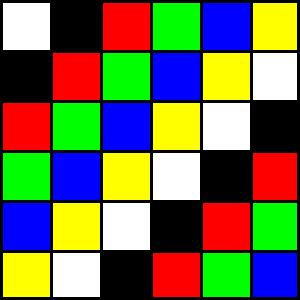
\includegraphics[height=6cm]{GRAPHICS/CYCLIC_6/Perm6_group_table_draw}
$$
\caption{\label{fig:C6:table}The group table of $C_6$}
\end{figure}
{\tt
\input GRAPHICS/THE_MAKEFILE/EXTRACTS/Cyclic_6_group_table.tex
}


\bigskip


Next, let us consider the symmetric group $\Sym(n)$. 
The following command creates $\Sym(3)$:
{\tt
\input GRAPHICS/THE_MAKEFILE/EXTRACTS/Symmetric_3.tex
}

The report is shown below:

\begin{mdframed}[style=MyFrame]
\input GRAPHICS/LATEX/report_group_sym_3.tex
\end{mdframed}


\bigskip


The following command produces a graphical representation 
of the group table of the symmetric group $\Sym(3)$, shown in Figure~\ref{fig:sym3:table}.
\begin{figure}
$$
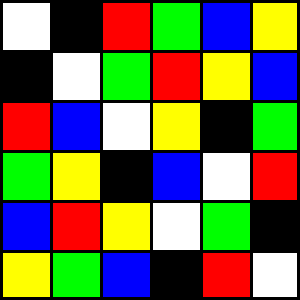
\includegraphics[height=6cm]{GRAPHICS/PERM3/Perm3_group_table_draw}
$$
\caption{\label{fig:sym3:table}The group table of $\Sym(3)$}
\end{figure}
{\tt
\input GRAPHICS/THE_MAKEFILE/EXTRACTS/Symmetric_3_group_table.tex
}



\bigskip



The next command produces a graphical representation 
of the elements of the symmetric group $\Sym(3)$, shown in Figure~\ref{fig:sym3:elts}.
\begin{figure}
$$
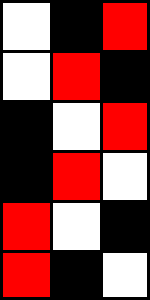
\includegraphics[height=6cm]{GRAPHICS/PERM3/Sym3_elts_matrix_draw}
$$
\caption{\label{fig:sym3:elts}The elements of $\Sym(3)$}
\end{figure}
{\tt
\input GRAPHICS/THE_MAKEFILE/EXTRACTS/Symmetric_3_elements.tex
}










\bigskip

Orbiter provides support for matrix groups and their various permutation representationes. 
For background information about the classical groups of matrices over finite fields, see cf.~\cite{Taylor1992}. 
Any group in Orbiter is associated with a permutation action. 
There can be multiple actions for the same group though.
Using homomorphisms of permutation groups, new actions can be formed from old actions. 
Basic group actions are  projective, affine, and general linear, as well as orthogonal, unitary and tensor product. 
Product actions can be defined also.
In order to establish a permutation representation, the elements (aka points) of the permutation domain 
need to be made available. One way would be to make a table of all elements in the permutation domain. 
However, this would be time and memory intensive. For this reason, a different technique is used that 
creates points only when needed. The way this works is that the permutation domain is encoded implicitly, 
using a fixed bijection to a suitable integer interval (zero based), called the domain. 
Whenever we want the $i$th point in the domain, we can call a function that produces it. 
Conversely, whenever we have a point, we can call a function that tells us what the associated index in the domain.
This is facilitated by two mutually inverse functions. 
The rank function turns a point into an index. 
The unrank function turns an index in the domain into a point. 
Rank and unrank functions are helpful because they eliminate the need for tables of all objects. 
The ranks lead to rather compact storage of objects in files. The objects can be reconstructed from the ranks.
%This way, we avoid storing tables and we make it easier for the computer to store points (namely 
%by storing the associated indices in the domain instead). 

%In addition, there are direct product action and tensor product actions.
%Group theoretic algorithms require short orbits to be efficient. 
%In order to create short orbits, Orbiter tags on an extra permutation domain for product and tensor actions.
%These extra permutation domains can be blended out later by forming a restricted action.

\bigskip

Let $V \simeq \bbF_q^n$
be a finite dimensional vector space over $\bbF_q$. 
The set of subspaces of $V$ form the projective geometry $\PG(n-1,q).$

\bigskip

Let $\pi$ be a projective space.
A collineation of a projective space $\pi$ 
is a bijective mapping from the points of $\pi$ to themselves  
which preserves collinearity. That is, a collineation $\varphi$ maps any 
three collinear points $P,Q,R$ 
to another collinear triple $\varphi(P), \varphi(Q), \varphi(R).$ 
The collineations form a group with respect to composition, the collineation group.
If $M$ is the matrix of an endomorphism, then $\Psi_M$ is the induced 
map on projective space. 
By considering the homomorphism $M \mapsto \Psi_M$, 
the group $\GL(n+1,q)$ of invertible endomorphisms becomes 
a subgroup of the group of collineations of $\PG(n,q).$ 
This is the projectivity group $\PGL(n+1,q).$ 
It is isomorphic to $\GL(n+1,q)/\bbF_q^\times.$ 
Another source of collineations is this: 
Let $\Phi \in \Aut(\bbF_q)$ be a field automorphism. Then 
$\Phi$ acts on projective space by sending 
$P(\bx)$ to $P(\bx\Phi).$ 
This map is another type of collineation, 
called automorphic collineation.
This way, $\Aut(\bbF_q)$ gives rise to a group of collineations.
If $q = p^h$ for some prime $p$ and some integer $h$ then 
$$
\Phi_0: \bbF_q \rightarrow \bbF_q, \; x \mapsto x^p
$$ 
is a generator for the cyclic group $C_h \simeq \Aut(\bbF_q).$ 
The collineation group 
of $\PG(n,q)$ ($n \ge 2$) is isomorphic 
to the semidirect product of the projectivity group and the 
automorphism group of the field. 
The collineation group is 
$\PGGL(n+1,q) = \PGL(n+1,q) \ltimes \Aut(\bbF_q).$
We use the following notation for elements of $\PGGL(n+1,q).$ 
Let $\Phi_0$ be a generator 
for $\Aut(\bbF_q)$ and let $M \in \GL(n+1,q).$ 
The map 
$$
(\Psi_M,\Phi_0^k): \PG(n,q) \rightarrow \PG(n,q), \; 
P(\bx) \mapsto P(\by), \quad \by = (\bx \cdot M)^{\Phi_0^k}
$$
is denoted as 
\begin{equation}\label{eqn:Mk}
M_k.
\end{equation}
The identity element is $I_0$, 
where $I$ is the identity matrix and $0$ is the residue class modulo $h.$
The rules for multiplication and inversion in the collineation group are given as
\begin{eqnarray}\label{eqn:MkNl}
M_k \cdot N_l &=& \Big(M \cdot N^{\Phi^{-k}}\Big)_{k+l},\\
\Big(M_k\Big)^{-1} &=& \Big(\Big(M^{-1}\Big)^{\Phi^{k}}\Big)_{-k}.
\end{eqnarray}
The affine group $\AGL(n,q)$ is the semidirect product of $\GL(n,q)$ with $\bbF_q^n.$ 
The affine semilinear group $\AGGL(n,q)$  is the semidirect product of $\AGL(n,q)$ with $\Aut(\bbF_q).$
The elements of $\AGGL(n,q)$ are triples 
$$
M_{\ba,k} := (M, \ba, k) \in \GL(n,q) \times \bbF_q^n \times \Aut(\bbF_q), 
$$
which act on $\bbF_q^n$:
$$
\Big(\bx, (M, \ba, k)\Big) \mapsto \big(\bx \cdot M + \ba\big)^{\Phi^k}.
$$
The multiplication in $\AGGL(n,q)$ is 
$$
M_{\ba,k}  \cdot N_{\bb,l} = (MN)_{\ba N^{\Phi^{-k}}+ \bb^{\Phi^{-k}},k+l}. 
$$
The inverse of an element is 
$$
\Big(M_{\ba,k} \Big)^{-1} = \Big( M^{-1}\Big)_{\ba^{\Phi^{k}} M^{-1},-k}.
$$

 


\bigskip

A correlation is a one-to-one mapping between the set of 
points and the set of hyperplanes which reverses incidence. 
So, if $\rho$ is a correlation and 
$P$ is a point and $\ell$ is a hyperplane then $P^\rho$ is a hyperplane and $\ell^\rho$ is 
a point and 
$$
\ell^\rho \in P^\rho \iff P \in \ell.
$$
A correlation of order two is called polarity.
The standard polarity is the map 
$$
\rho:  \cP \leftrightarrow \cL, \;P(\bx) \leftrightarrow [\bx].
$$





\bigskip

A group $G$ can act on $V$ in one of the types listed in Table~\ref{tab:actions}.
\begin{table}
	\begin{center}
	{\renewcommand{\arraystretch}{2.1}
	\begin{tabular}{|c|c|c|}
		\hline
		Type & Perm. Domain & Degree \\
		\hline
		\hline
		General linear $\GL(n,q)$ & all vectors of $V$ & $q^n$ \\
		\hline
		Affine $\AGL(n,q)$ & all vectors of $V$ & $q^n$ \\
		\hline
		Projective $\PGL(n,q)$& ${\frak Gr}_1(V)$ & $\frac{q^n-1}{q-1}$ \\
		\hline
		Wreath product $\GL(d,q) \wr \Sym(n)$ & ${\frak Gr}_1((\bbF_q^d)^{\otimes n})$ extended &  $n+nq^d+ \frac{q^{d^n}-1}{q-1}$\\
		\hline
		Orthogonal $\PGO(n,q)$& $Q(V)$ &  $\displaystyle \frac{q^{n-1}-1}{q-1}$\\
		\hline
		Orthogonal $\PGO^+(n,q)$& $Q^+(V)$ &  $\displaystyle \frac{(q^{n/2}-1)(q^{(n-2)/2}+1)}{q-1}$ \\
		\hline
		Orthogonal $\PGO^-(n,q)$& $Q^-(V)$ &  $\displaystyle \frac{(q^{n/2}+1)(q^{(n-2)/2}-1)}{q-1}$\\
		\hline
		\end{tabular}}
	\end{center}
	\caption{\label{tab:actions}Basic actions}
	\end{table}
One can create a matrix group over a finite field $\bbF_q$ is created as described in  in two steps. 
In the first step, the field $\bbF_q$ is created as described in Sections~\ref{sec:finite:fields} and~\ref{sec:extension:fields}.
The field is stored in the symbol table.
Then, the group is created using the symbolic label for the field.
The basic types of matrix groups in Orbiter 
are listed in Table~\ref{tab:matrixgroups}.
\begin{table}
\begin{center}
\begin{tabular}{|l|c|c|}
\hline
Command & Arguments & Group \\
\hline
\hline
\verb'-GL' & $n$ $q$ & $\GL(n,q)$ \\
\hline
\verb'-GGL' & $n$ $q$ & $\GGL(n,q)$ \\
\hline
\verb'-SL' & $n$ $q$ & $\SL(n,q)$ \\
\hline
\verb'-SSL' & $n$ $q$ & $\SSL(n,q)$ \\
\hline
\verb'-PGL' & $n$ $q$ & $\PGL(n,q)$ \\
\hline
\verb'-PGGL' & $n$ $q$ & $\PGGL(n,q)$ \\
\hline
\verb'-PSL' & $n$ $q$ & $\PSL(n,q)$ \\
\hline
\verb'-PSSL' & $n$ $q$ & $\PSSL(n,q)$ \\
\hline
\verb'-AGL' & $n$ $q$ & $\AGL(n,q)$ \\
\hline
\verb'-AGGL' & $n$ $q$ & $\AGGL(n,q)$ \\
\hline
\verb'-ASL' & $n$ $q$ & $\ASL(n,q)$ \\
\hline
\verb'-ASSL' & $n$ $q$ & $\ASSL(n,q)$ \\
\hline
\verb'-PGO' & $n$ $q$ & $\PGO(n,q)$ \\
\hline
\verb'-PGOp' & $n$ $q$ & $\PGO^+(n,q)$ \\
\hline
\verb'-PGOm' & $n$ $q$ & $\PGO^-(n,q)$ \\
\hline
\verb'-PGGO' & $n$ $q$ & $\PGGO(n,q)$ \\
\hline
\verb'-PGGOp' & $n$ $q$ & $\PGGO^+(n,q)$ \\
\hline
\verb'-PGGOm' & $n$ $q$ & $\PGGO^-(n,q)$ \\
\hline
\verb'-GL_d_q_wr_Sym_n' & $d$ $q$ $n$ & $\GL(d,q) \wr \Sym(n)$ \\
\hline
\end{tabular}
\end{center}
\caption{\label{tab:matrixgroups}Basic types of Orbiter matrix groups}
\end{table}


\bigskip


For instance, 
{\tt
\input GRAPHICS/THE_MAKEFILE/EXTRACTS/PGL_4_2.tex
}
creates the group $\PGL(4,2)$ acting on the $15$ elements of ${\frak Gr}_1(\bbF_2^4)$. 
At first, the field $\bbF_2$ is created. 
Secondly, the group $G=\PGL(3,2)$ is created using the previously created field $\bbF_2$, 
and a report is generated.
The report gives information about the permutation group action, 
including the underlying field and the projective geometry.
\begin{mdframed}[style=MyFrame]
\input GRAPHICS/LATEX/report_group_PGL_4_2.tex
\end{mdframed}



\bigskip




We use the following Orbiter command creates $\PGL(4,2)$ again.
The command invokes two activities. 
The first creates a latex report for the group in the file \verb'PGL_4_2_report.tex'.
The second activity exports the permutation representation in Orbiter makefile format.
{\tt
\input GRAPHICS/THE_MAKEFILE/EXTRACTS/PGL_4_2_export.tex
}
The file \verb'PGL_4_2.makefile' is created:
{\tt
\input GRAPHICS/THE_MAKEFILE/EXTRACTS/PGL_4_2_generated.tex
}
This command can be used to recreate the group as permutation group directly.
This group will be considered again in Section~\ref{sec:lineargroups} below.
The permutation representation itself is stored in the file \verb'PGL_4_2_gens.csv':
\begin{verbatim}
Row,C0,C1,C2,C3,C4,C5,C6,C7,C8,C9,C10,C11,C12,C13,C14
0,0,1,2,9,14,5,6,7,8,3,11,10,13,12,4
1,0,1,2,10,13,5,6,7,8,11,3,9,14,4,12
2,0,1,2,12,11,5,6,7,8,13,14,4,3,9,10
3,0,1,3,2,4,5,9,10,11,6,7,8,12,13,14
4,0,2,1,3,4,6,5,7,8,9,12,13,10,11,14
5,1,0,2,3,4,5,7,6,8,10,9,11,12,14,13
END
\end{verbatim}

\bigskip



The command
{\tt
\input GRAPHICS/THE_MAKEFILE/EXTRACTS/L_5_3.tex
}
creates $\PSL(5,3)$ of order $237783237120.$

\bigskip


The command 
{\tt
\input GRAPHICS/THE_MAKEFILE/EXTRACTS/PSP_4_4.tex
}
creates the symplectic group $\PSp(4,4)$ of order $979200.$


\bigskip



The command 
{\tt
\input GRAPHICS/THE_MAKEFILE/EXTRACTS/PGO_5_2.tex
}
creates the group $\PGO(5,2)$ acting on the 15 points of the $Q(4,2)$ quadric. 
The following latex report is produced:
\begin{mdframed}[style=MyFrame]
\input GRAPHICS/LATEX/report_group_PGO_5_2.tex
\end{mdframed}


\bigskip


The symplectic group $\PSp(6,2)$  can be created using the following command: 
{\tt
\input GRAPHICS/THE_MAKEFILE/EXTRACTS/PSP_6_2.tex
}

\bigskip

The group $\PGO(7,2)$, isomorphic to  $\PSp(6,2)$, can be created using the following command: 
{\tt
\input GRAPHICS/THE_MAKEFILE/EXTRACTS/PGO_7_2.tex
}


There are many ways to create subgroups of a group.
Table~\ref{tab:subgroups} lists some commands to do so.
\begin{table}
\begin{center}
\begin{tabular}{|p{4cm}|c|p{8cm}|}
\hline
Command & Arguments & Purpose \\
\hline
\hline
\verb'-Janko1' &  & first Janko group, needs $\PGL(7,11)$ \\
\hline
\verb'-monomial' &  & subgroup of monomial matrices \\
\hline
\verb'-diagonal' &  & subgroup of diagonal matrices \\
\hline
\verb'-null_polarity_' \verb'group' & & null polarity group \\
\hline
\verb'-symplectic_group' & & symplectic group \\
\hline
\verb'-singer' & $k$ & subgroup of index $k$ in the Singer cycle \\
\hline
\verb'-singer_and_' \verb'frobenius' & $k$ & subgroup of index $k$ in the Singer cycle, 
extended by the Frobenius automorphism of $\bbF_{q^n}$ over $\bbF_q$ \\
\hline
\verb'-borel_upper' &  & Borel subgroup of upper triangular matrices \\
\hline
\verb'-borel_lower' &  & Borel subgroup of lower triangular matrices \\
\hline
\verb'-identity_group' &  & identity subgroup \\
\hline
\verb'-subgroup_from_' \verb'file' & $f$ $l$ & read subgroup from file $f$ and give it the label $l$\\
\hline
\verb'-orthogonal' & $\epsilon$ & orthogonal group $O^\epsilon(n,q)$, 
with $\epsilon  \in \{ \pm 1 \}$ when $n$ is even\\
\hline
\verb'-subgroup_by_' \verb'generators' & $l$ $o$ $n$ $s_1$ $\ldots$ $s_n$ & Generate a subgroup from generators. 
The label ``l'' is used to denote the subgroup; $o$ is the order of the subgroup; 
$n$ is the number of generators and $s_1$, $\ldots$, $s_n$ 
are the generators for the subgroup in vector form. \\
\hline
\end{tabular}
\end{center}
\caption{\label{tab:subgroups}Commands for creating subgroups}
\end{table}



We start with an example of an explicit permutation group using a known base and strong generating set, 
using the \verb'bsgs' command.
Here is the cyclic group of order 13 acting on the permutation domain $[0,12]$. 
The base is $(0)$. When creating a group, we supply a label in ascii text and in tex. 
Then we specify the degree of the action, and the group order. 
After that, we specify the number of generators and the generators themselves.
The labels will be used in reports about the group, for instance. 
{\tt
\input GRAPHICS/THE_MAKEFILE/EXTRACTS/GEN_C13.tex
}
{\tt
\input GRAPHICS/THE_MAKEFILE/EXTRACTS/C13.tex
}
The makefile variable \verb'GEN_C13' is used to define the generator of the group, which is 
the cycle 
$$
(0,1,2,3,4,5,6,7,8,9,10,11,12).
$$
The generator is given in list notation, which is the second row in the array
$$
\left[
\begin{array}{ccccccccccccc}
0&1&2&3&4&5&6&7&8&9&10&11&12\\
1&2&3&4&5&6&7&8&9&10&11&12&0\\
\end{array}
\right].
$$
The command creates the group from the known base $0$. 
After that, several activities are invoked.
Specifically, these are group theoretic activities. 
They will be discussed in more detail in Section~\ref{sec:group:theoretic:activities}.

\bigskip

Let us take a closer look at the three activities performed in this example.
The \verb'-export_orbiter' command 
exports the group in Orbiter makefile format.
The file \verb'C13.makefile' is generated,
which can be used to recreate the permutation group in an Orbiter makefile. 
Here is the content of the file:
{\tt
\input GRAPHICS/THE_MAKEFILE/EXTRACTS/C13_generated.tex
}

\bigskip

The activity \verb'-report'
produces a report for the cyclic group, shown below:

\begin{mdframed}[style=MyFrame]
\input GRAPHICS/LATEX/report_subgroup_C13.tex
\end{mdframed}

\bigskip


The command  \verb'-save_elements_csv'
creates a csv file containing all group elements. 
Each group element is listed one-by-one, using the list notation of permutations.
The csv file \verb'C13_elts.csv' has the following content:
\begin{verbatim}
Row,Element
0,"0,1,2,3,4,5,6,7,8,9,10,11,12"
1,"1,2,3,4,5,6,7,8,9,10,11,12,0"
2,"2,3,4,5,6,7,8,9,10,11,12,0,1"
3,"3,4,5,6,7,8,9,10,11,12,0,1,2"
4,"4,5,6,7,8,9,10,11,12,0,1,2,3"
5,"5,6,7,8,9,10,11,12,0,1,2,3,4"
6,"6,7,8,9,10,11,12,0,1,2,3,4,5"
7,"7,8,9,10,11,12,0,1,2,3,4,5,6"
8,"8,9,10,11,12,0,1,2,3,4,5,6,7"
9,"9,10,11,12,0,1,2,3,4,5,6,7,8"
10,"10,11,12,0,1,2,3,4,5,6,7,8,9"
11,"11,12,0,1,2,3,4,5,6,7,8,9,10"
12,"12,0,1,2,3,4,5,6,7,8,9,10,11"
END
\end{verbatim}



\bigskip



It is possible to create a permutation group as a subgroup of the symmetric group, 
using the known base for the symmetric group.
Because the base of the symmetric group is large, 
this way of creating the group 
is less efficient than creating the group with a known (small) base.
Here is an example. We create $C_{13}$ as a subgroup of $\Sym(13)$.
{\tt
\input GRAPHICS/THE_MAKEFILE/EXTRACTS/C13_as_subgroup.tex
}
The \verb'subgroup_by_generators' command will be discussed in more detail in Section~\ref{sec:subgroups}.

\bigskip




For instance, the command
{\tt
\input GRAPHICS/THE_MAKEFILE/EXTRACTS/J1.tex
}
creates the first Janko group as a subgroup of $\PGL(7,11).$ 

\bigskip

The command 
{\tt
\input GRAPHICS/THE_MAKEFILE/EXTRACTS/PGL_3_11_singer.tex
}
creates a subgroup of the Singer cycle of order 7.
The Singer cycle in $\GL(d,q)$ is a generator for a subgroup of order $q^d-1$. 
It induces an element of order  $\frac{q^d-1}{q-1}$ on the associated projective geometry $\PG(d-1,q).$
The additional integer parameter $k$ after the $\verb'-singer'$ command  is used to 
create  the subgroup of index $k$ of the Singer cycle.

\bigskip


The command 
{\tt
\input GRAPHICS/THE_MAKEFILE/EXTRACTS/PGL_3_11_singer_and_frobenius.tex
}
creates a subgroup of index 19 of the Singer cycle of $\PG(2,11)$, 
extended by a group of order $3$ 
that arises from the field extension $\bbF_{11}^3$ over $\bbF_{11}.$ 
The group created by this command has order $21$.


\bigskip




The quaternion group is a group of order $8$ generated by 
the following matrices over $\bbR$:
$$
i = 
\left[
\begin{array}{rr}
1&1\\
1&-1\\
\end{array}
\right], \quad
j = 
\left[
\begin{array}{rr}
-1&1\\
1&1\\
\end{array}
\right], \quad
k = 
\left[
\begin{array}{rr}
0&-1\\
1&0\\
\end{array}
\right].
$$
It is isomorphic to a subgroup of $\SL(2,3).$
The Orbiter command
{\tt
\input GRAPHICS/THE_MAKEFILE/EXTRACTS/quaternion.tex
}
creates the group. 
The command produces the list of group elements shown below.
\begin{mdframed}[style=MyFrame]
\input GRAPHICS/LATEX/report_subgroup_quaternion.tex
\end{mdframed}
The group table is created as csv file:
\begin{mdframed}[style=MyFrame]
\input GRAPHICS/LATEX/report_group_quaternion_table.tex
\end{mdframed}


\bigskip

The group of the cube can be created over the field $\bbF_3$:
{\tt
\input GRAPHICS/THE_MAKEFILE/EXTRACTS/cube_group.tex
}
The tetrahedral subgroup can be created as well:
{\tt
\input GRAPHICS/THE_MAKEFILE/EXTRACTS/tetra_group.tex
}
The Hesse group of order 216 extended by the automorphism group of the field 
can be created in $\PG(3,4)$
{\tt
\input GRAPHICS/THE_MAKEFILE/EXTRACTS/GENERATORS_HESSE_GROUP.tex
}
{\tt
\input GRAPHICS/THE_MAKEFILE/EXTRACTS/Hesse_group.tex
}
The group has order 432.

\bigskip



The Weyl group of type $E_8$ can be generated as a subgroup of $\GL(8,3)$ 
using the following command:
{\tt
\input GRAPHICS/THE_MAKEFILE/EXTRACTS/GENERATORS_WEYL_GROUP_E8.tex
}
{\tt
\input GRAPHICS/THE_MAKEFILE/EXTRACTS/Weyl_E8.tex
}
A latex report is generated in the file \verb'GL_8_3_Subgroup_Weyl_E8_696729600_report.tex'.
This command uses generators found by Gabi Nebe:
$$
\verb'http://www.math.rwth-aachen.de/~Gabriele.Nebe/LATTICES/E8.b.html'
$$


\bigskip


We can test if a group is a subgroup of another. 
In the following example, we test whether 
$\PGO^+(6,2)$ is a subgroup of $\PSp(6,2)$. 
The fact that it is depends on the choice of forms 
associated with the groups and on the fact that the characteristic is two.
{\tt
\input GRAPHICS/THE_MAKEFILE/EXTRACTS/test_subgroup.tex
}
Since the subgroup index is small (36), we create a set of 
coset representatives using the following command:
{\tt
\input GRAPHICS/THE_MAKEFILE/EXTRACTS/coset_reps.tex
}
The coset representatives are written to a csv file.
The (shortened) list of coset representatives in latex is:
\begin{mdframed}[style=MyFrame]
\input GRAPHICS/LATEX/report_group_coset_reps_36.tex
\end{mdframed}

\bigskip


The following command reads the vector of coset representatives from the file just created.
{\tt
\input GRAPHICS/THE_MAKEFILE/EXTRACTS/coset_reps_read.tex
}


It is sometimes necessary to control the finite field 
that is used in the construction of a matrix group.
For prime fields, this is not an issue. 
For extension fields, the choice of polynomial does matter, as 
the generators depend on specific choices made for the finite field. 
Magma and GAP use Conway polynomials, which are difficult to compute.
Orbiter has a built-in table of primitive polynomials. 
As explained in Section~\ref{sec:extension:fields},
Orbiter allows to specify the polynomial that should be used to create the finite field.
The next example shows an instance where choosing 
the polynomial is important. We are recreating a group 
from the electronic Atlas on finite simple groups~\cite{Atlas3}.

\bigskip

The electronic Atlas of finite simple groups~\cite{Atlas3} 
lists generators for $U_3(3)$ as $3 \times 3$ matrices over the field $\bbF_9$
using the following short Magma~\cite{Magma} program:
\begin{verbatim}
F<w>:=GF(9);
x:=CambridgeMatrix(1,F,3,[
"164",
"506",
"851"]);
y:=CambridgeMatrix(1,F,3,[
"621",
"784",
"066"]);
G<x,y>:=MatrixGroup<3,F|x,y>;
\end{verbatim} 
The generators are given using the Magma command \verb'CambridgeMatrix', 
which allows for more efficient coding of field elements.
The field elements are coded as base-3 integers (like in Orbiter) 
with respect to the Magma version of $\bbF_9.$ 
The polynomial for $\bbF_9$ can be determined using the 
following Magma command, 
which can be typed into Magma (or 
the free Magma online calculator at~\cite{MagmaOnline}):
\begin{verbatim}
F<w>:=GF(9);
print DefiningPolynomial(F);
\end{verbatim}
It results in
\begin{verbatim}
$.1^2 + 2*$.1 + 2
\end{verbatim}
which is the Magma way of printing the polynomial $X^2+2X+2.$ 
If $\alpha$ is a root of the polynomial over $\bbF_3$, then
$$
\alpha^2 = \alpha+1.
$$
The coefficient vector of 
the polynomial is $(1,2,2).$ 
As an integer written in base-3, we 
obtain 
$$
1\cdot 3^2 + 2 \cdot 3 + 2 = 17.
$$
%The command  
%\begin{verbatim}
%-finite_field -q 9 -override_polynomial "17"  -end
%\end{verbatim}
%can be used to create $\bbF_9$ using this polynomial.
%The command 
%\begin{verbatim}
%-define F -finite_field -q 9 -override_polynomial "17" -end
%\end{verbatim}
%creates a symbolic variable $F$ for this specific field $\bbF_9$.
%In order to create the linear group over this field, the command 
%\begin{verbatim}
%-linear_group -PGL 3 F -end
%\end{verbatim}
%can be used, where the second argument after 
%the \verb'-PGL' command references the field $\bbF_9$ 
%that we just created through its symbolic name.
The desired subgroup can now be created using the command
{\tt
\input GRAPHICS/THE_MAKEFILE/EXTRACTS/U_3_3.tex
}
Group theoretic activities 
will be discussed in Section~\ref{sec:group:theoretic:activities}.

\bigskip

As an example of a large group, consider the Conway group ${\rm Co}_3.$ 
Following~\cite{SuleimanWilson1997}, the group can be generated using two 
matrices of dimension $22$ over $\bbF_2$. 
We use the makefile variables to give each generator in compact form. 
Then we define vectors for each of the generators. 
We concatenate the two generators to 
form one long vector, 
which is passed to the \verb'-subgroup_by_generators' command.
Finally, we create a report for the group.
{\tt
\input GRAPHICS/THE_MAKEFILE/EXTRACTS/CONWAY_GEN1.tex
}
{\tt
\input GRAPHICS/THE_MAKEFILE/EXTRACTS/CONWAY_GEN2.tex
}
{\tt
\input GRAPHICS/THE_MAKEFILE/EXTRACTS/Co3.tex
}


\bigskip

The next example creates the Ree group 
in 7 dimensions over the field $\bbF_{27}$. 
Again, we use makefile variables to specify the 
two generators as $7 \times 7$ matrices over $\bbF_{27}$ 
and concatenate them, 
before passing them to the \verb'-subgroup_by_generators' command.
{\tt
\input GRAPHICS/THE_MAKEFILE/EXTRACTS/Ree_gen1.tex
}
{\tt
\input GRAPHICS/THE_MAKEFILE/EXTRACTS/Ree_gen2.tex
}
{\tt
\input GRAPHICS/THE_MAKEFILE/EXTRACTS/Ree_27.tex
}
 
It is possible to create new group actions from old.
Table~\ref{tab:modifier} lists Orbiter commands to do so.
\begin{table}
\begin{center}
\begin{tabular}{|p{4cm}|p{3cm}|p{8cm}|}
\hline
Command & Arguments & Purpose \\
\hline
\hline
\verb'-wedge' &  & action on the exterior square \\
\hline
\verb'-wedge_detached' &  & action on the exterior square. Unlike \verb'-wedge', this command does not establish the homomorphism to the original group. Instead, the group is created as subgroup of the larger general linear group.\\
\hline
\verb'-PGL2OnConic' &  & induced action of $\PGL(2,q)$ on the conic in the plane $\PG(2,q)$ \\
\hline
\verb'-subfield_' \verb'structure_action' & $s$ & action by field reduction to the subfield of index $s$\\
\hline
\verb'-on_k_subspaces' & $k$ & induced action on $k$ dimensional subspaces \\
\hline
\verb'-on_tensors' &  & induced action of $\GL(d,q) \wr \Sym(n)$ on the tensor space \\
\hline
\verb'-on_rank_one_' \verb'tensors' &  & induced action of $\GL(d,q) \wr \Sym(n)$ on the tensor space \\
\hline
\verb'-restricted_action' & $s$ & restricted action on the set $s$ \\
\hline
\end{tabular}
\end{center}
\caption{\label{tab:modifier}Commands for creating new actions from old}
\end{table}
For instance, the command 
{\tt
\input GRAPHICS/THE_MAKEFILE/EXTRACTS/T3_on_tensors.tex
}
creates the group $\GL(2,2) \wr \Sym(3)$ acting on the $255$ elements 
of $\PG(7,2)$ which are identified with the 
tensors of type $(2,2,2)$ over $\bbF_2.$  
Elements of this group are denoted in the notation of the semidirect product. 
A vector of elements in the linear group is followed by a permutation of the components. 
%It is also important to observe that the stabilizer chain is very long and has short subgroup indices. 
%This is because $\GL(2,2) \wr \Sym(3)$ is originally created on a larger permutation domain. 
%This larger permutation domain allows for short orbits, making the implementation more efficient.
\begin{mdframed}[style=MyFrame]
\input GRAPHICS/LATEX/report_group_T3_on_tensor.tex
\end{mdframed}
It is also possible to restrict the action on all rank-one tensors, as the following example shows:
{\tt
\input GRAPHICS/THE_MAKEFILE/EXTRACTS/T3r1.tex
}
This creates an action of degree 27. 
Because the degree is small, 
the Orbiter report shows all points in the permutation domain.
\begin{mdframed}[style=MyFrame]
\input GRAPHICS/LATEX/report_group_T3_on_tensor_rank_one.tex
\end{mdframed}


\bigskip

The group of a conic is isomorphic to the group of the projective line. 
This isomorphism from the group of the projective line to the group of the conic can be realized using the 
command \verb'PGL2OnConic'. 
The action is changed using the induced action on the Veronese variety. 
The group elements are still represented as $2 \times 2$ matrices.
Here is an example. 
We create the collineation group $\PGGL(2,8)$ of $\PG(1,8)$ and act on $\PG(2,8)$:
{\tt
\input GRAPHICS/THE_MAKEFILE/EXTRACTS/PGGL_2_8_on_conic.tex
}
This produces the following report. 
The generators are elements of $\PGGL(2,8)$ acting on $\PG(2,8).$ 
The first basic orbit is the conic itself and all other basic orbits are subsets of it.
\begin{mdframed}[style=MyFrame]
\input GRAPHICS/LATEX/report_group_PGGL_2_8_on_conic.tex
\end{mdframed}

\bigskip


In the following example, we will demonstrate two types of induced actions. 
One is the action induced on $k$-dimensional subspaces. 
The second is the restricted action on an invarant subset.
The example we show is related to cubic surfaces.
At first, we create the Eckardt surface in $PG(3,13)$ from 
the arc 
$$
\{0,1,2,3,43,113\}. 
$$
Then we export the set of $45$ tritangent planes to file 
and we produce a report about the surface and its automorphism group.
The next command creates the stabilizer of the surface 
from the generators given in the report, 
creates the induced action on planes, 
and restricts the action to the 45 tritangent planes stored in the file.
Here is the fill command sequence, including a makefile variable 
for the generators of the stabilizer of the surface:
{\tt
\input GRAPHICS/THE_MAKEFILE/EXTRACTS/SURFACE_Q13_STAB_GENS.tex
}
{\tt
\input GRAPHICS/THE_MAKEFILE/EXTRACTS/surface_q13_Eckardt_on_tritangent_planes.tex
}


\bigskip




Once a group has been created as in Section~\ref{sec:lineargroups}, 
a group theoretic activity can be performed.  
For this purpose, Orbiter provides the \verb'-group_theoretic_activity' option. 
Tables~\ref{tab:grouptasks} and~\ref{tab:grouptasks2} 
list the possible commands that can come after it. 
\begin{table}
\begin{center}
\begin{tabular}{|p{4cm}|p{3cm}|p{8cm}|}
\hline
Command & Arguments & Purpose \\
\hline
\hline
\verb'-apply' & $a$ $s$ & 
Applies the group element given by the coded vector $s$ to the element $a$. \\
\hline
\verb'-multiply' & $s_1$ $s_2$ & 
Multiplies group elements $s_1$ and $s_2$, assuming the elements are given in coded form. Produces a latex report. \\
\hline
\verb'-inverse' & $s$ & 
Computes the inverse of $s$, which is given in coded form. Produces a latex report. \\
\hline
\verb'-consecutive_powers' & $s$ $n$ & 
Computes all powers $s^i$ for $i=1,\ldots,n.$ $s$ is given in coded form. Produces a latex report. \\
\hline
\verb'-raise_to_the_power' & $s$ $n$ & 
Computes the $n$-th power of of $s$, which is given in coded form. Produces a latex report. \\
\hline
\verb'-export_orbiter' &  & 
Exports the group to Orbiter. \\
\hline
\verb'-export_gap' &  & 
Exports the group to GAP~\cite{GAP}. \\
\hline
\verb'-export_magma' &  & 
Exports the group to Magma~\cite{Magma}. \\
\hline
\verb'-search_element_' \verb'of_order' & $i$ & 
Finds all elements of order $i$ in the group ($i \in {\mathbb N}$). \\
\hline
\verb'-element_rank' & $s$ & 
Determines the rank of the group element $s$ in the given group. $s$ is given in coded form.\\
\hline
\verb'-element_unrank' & $r$ & 
Produces the group element whose rank is $r$. \\
\hline
\verb'-find_singer_cycle' &  & 
Finds all Singer cycles whose matrix is a companion matrix. \\
\hline
\verb'-poset_classifi' \verb'cation_control' & see Table~\ref{tab:pc:options} & 
Poset classification options. The argument list must be terminated with \verb'-end' \\
\hline
\verb'-classes_based_' \verb'on_normal_form' & & \\
\hline
\verb'-group_table' & & 
Stores the group table as csv-file. \\
\hline
\verb'-report' & & 
Produce a latex report about the group. \\
\hline
\verb'-sylow' & & 
Include Sylow subgroups in the report (requires \verb'-report'). \\
\hline
\verb'-print_elements' & & 
Produces a printout of all group elements. \\
\hline
\verb'-print_elements_tex' & & 
Produces a latex report of all group elements. \\
\hline
\verb'-order_of_products' & $g_1 \ldots g_n$ & 
Creates a table of the orders of all products $g_ig_j$, $1 \le i,j \le n.$\\
\hline
\end{tabular}
\end{center}
\caption{\label{tab:grouptasks}Group theoretic activities (Part 1)}
\end{table}
\begin{table}
\begin{center}
\begin{tabular}{|p{4cm}|p{3cm}|p{8cm}|}
\hline
Command & Arguments & Purpose \\
\hline
\hline
\verb'-classify_arcs' & description & 
Classify arcs in geometries. See Section~\ref{sec:arcs}.\\
\hline
\verb'-linear_codes' & $d$ $n_{\max}$ & 
Classify linear codes with prescribed minimum distance $d$. 
Assumes that the group is $\PGL(r,q)$ or $\PGGL(r,q).$ 
For each $n \le n_{\max}$, the $[n,k, \ge d]$ codes are classified with $n-k=r$. 
See Section~\ref{sec:coding}. \\
\hline
\verb'-tensor_classify' & $d$ & Classifies tensors of tensor-rank at most $d.$ \\
\hline
\verb'-tensor_' \verb'permutations' &  & 
Computes the permutation representation of generators of wreath product. \\
\hline
\verb'-reverse_iso' \verb'morphism_exterior' \verb'_square' & & 
Given a set of generators of a subgroup of $\PGO^+(6,q)$ as $6\times 6$ matrixes, 
compute the inverse image of the generators in $\PGL(4,q)$ (if possible).\\
\hline
\verb'-classify_cubic_' \verb'curves' & descr & 
Classifies cubic curves. 
Expects an arc description options as in Table~\ref{tab:arcs}. \\
\hline
\end{tabular}
\end{center}
\caption{\label{tab:grouptasks2}Group theoretic activities (Part 2)}
\end{table}

\bigskip

The command
{\tt
\input GRAPHICS/THE_MAKEFILE/EXTRACTS/PGL_3_2_elements.tex
}
creates all elements of $\PGL(3,2)$ and writes them into the file \verb'PGL_3_2_elements.csv'.

\bigskip


The command
{\tt
\input GRAPHICS/THE_MAKEFILE/EXTRACTS/Sym_3_elements.tex
}
creates a tree of the elements of $\Sym(3)$ (see Fig~\ref{fig:sym:3:tree}). 
The leaves are ordered lexicographically.
\begin{figure}
$$
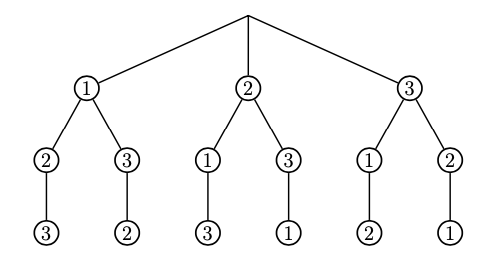
\includegraphics[width=11cm]{GRAPHICS/PERM3/sym_3_tree}
$$
\caption{\label{fig:sym:3:tree}The elements of $\Sym(3)$ in lex-order}
\end{figure}

\bigskip



It is possible to compute all powers of a fixed element, as in the following command:
{\tt
\input GRAPHICS/THE_MAKEFILE/EXTRACTS/Cycle_12_power.tex
}
We create the 12 powers of the cycle 
$$
(0,1,2,3,4,5,6,7,8,9,10,11).
$$
The output is
\begin{mdframed}[style=MyFrame]
\input GRAPHICS/LATEX/report_group_element_powers.tex
\end{mdframed}


\bigskip


The command
{\tt
\input GRAPHICS/THE_MAKEFILE/EXTRACTS/PGL_3_4_singer.tex
}
finds all Singer cycles in $\PGL(3,4)$ 
whose matrix is the companion matrix of a polynomial. 
The first one found is 
\begin{mdframed}[style=MyFrame]
\input GRAPHICS/LATEX/report_group_singer.tex
\end{mdframed}
whose projective order is $21.$ 
Here, we are using the numeric form of field elements, 
so $2$ is $\omega$ and $3$ is $\omega+1.$

\bigskip

Suppose we want to multiply two elements in a group. 
The following command shows an example in $\GL(2,8).$ 
We multiply the elements coded by 0,1,2,3 and 4,5,6,7:
{\tt
\input GRAPHICS/THE_MAKEFILE/EXTRACTS/GL_2_8_multiply.tex
}
The output is
\begin{mdframed}[style=MyFrame]
\input GRAPHICS/LATEX/report_group_multiply_GL_2_8.tex
\end{mdframed}
Note that the output shows the codings of the three group elements. 
This way, the result of this computation can be processed further easily.
The same example over $\bbF_7$, noting that $7 \equiv 0 \mod 7$ is:
{\tt
\input GRAPHICS/THE_MAKEFILE/EXTRACTS/GL_2_7_multiply.tex
}
The output is
\begin{mdframed}[style=MyFrame]
\input GRAPHICS/LATEX/report_group_multiply_GL_2_7.tex
\end{mdframed}
We can compute the inverse of a  group element:
{\tt
\input GRAPHICS/THE_MAKEFILE/EXTRACTS/GL_2_7_inv.tex
}
The output is
\begin{mdframed}[style=MyFrame]
\input GRAPHICS/LATEX/report_group_inverse_GL_2_7.tex
\end{mdframed}
We can raise a group element to a power:
{\tt
\input GRAPHICS/THE_MAKEFILE/EXTRACTS/GL_2_7_power.tex
}
The output is
\begin{mdframed}[style=MyFrame]
\input GRAPHICS/LATEX/report_group_power_GL_2_7.tex
\end{mdframed}

\bigskip


The next example computes the action of a specific group element on the set of planes through a line. 
The planes have been computed in Section~\ref{sec:grassmannian}.
{\tt
\input GRAPHICS/THE_MAKEFILE/EXTRACTS/on_planes.tex
}
The output is
\begin{mdframed}[style=MyFrame]
\input GRAPHICS/LATEX/report_group_on_planes.tex
\end{mdframed}

Through its interface to Magma~\cite{Magma}, Orbiter can perform group theoretic computations. 
Table~\ref{tab:grouptasks:magma} list the group theoretic commands that rely on Magma.
\begin{table}
\begin{center}
\begin{tabular}{|p{4cm}|p{3cm}|p{8cm}|}
\hline
Command & Arguments & Purpose \\
\hline
\hline
\verb'-classes' & & Compute a report of the conjugacy classes of elements. \\
\hline
\verb'-centralizer_' \verb'of_element' & label coding & Compute the centralizer of the coded group element, using label to create file names. \\
\hline
\verb'-normalizer_' \verb'of_cyclic_subgroup' & label $s$ & 
Compute the normalizer of the cyclic subgroup generated by the element $s$. \\
\hline
\verb'-normalizer' & & Compute the normalizer of a subgroup in the larger group. \\
\hline
\end{tabular}
\end{center}
\caption{\label{tab:grouptasks:magma}Group theoretic activities based on Magma}
\end{table}
The communication to and from magma happens through files. This is a three step process: 
An Orbiter session receives a command to compute the conjugacy classes of a group.
The Orbiter session writes a magma file. 
This file is read and executed by Magma. 
Magma writes a second file containing the conjugacy classes in coded form.
Another Orbiter session reads the magma output file, decodes the information and produces the desired list of conjugacy classes. 
A latex report is written containg the classes, as well as related information regarding centralizers and normalizers. 

\bigskip

For instance, the three-step command sequence  
{\tt
\input GRAPHICS/THE_MAKEFILE/EXTRACTS/PGGL_2_4_classes.tex
}
computes the classes of elements in $\PGGL(2,4)$
using Orbiter-Magma-Orbiter. 
The first Orbiter command produces the file \verb'PGGL_2_4_classes.magma'.
The magma command reads this file and produces the file \verb'PGGL_2_4_classes_out.txt'. 
The second Orbiter command reads the file \verb'PGGL_2_4_classes_out.txt' and produces the latex report 
\verb'PGGL_2_4_classes_out.tex'.
%together with the normalizers of the associated cyclic subgroups generated by the class representatives.
%Note that the  orbiter command is repeated twice, with one Magma command in between.
%Upon the first invocation, the file  \verb'PGGL_2_4_classes.magma' is written. 
%The magma command produces the file \verb'PGGL_2_4_classes_out.txt', 
%which is used during the second invocation of the Orbiter command to create 
%the latex file containing the conjugacy classes in the group. 
%This command sequence may have to be changed depending on the location of 
%magma on the system. 
%Also, the open command to display a pdf file is Macintosh specific.

\bigskip


The report produced by Orbiter is too long to be reproduced here fully. 
Let us look at just one conjugacy class. 
Here is the output for class 1 / 7 (numbering starts from 0, so this is the second class):

\bigskip


\begin{mdframed}[style=MyFrame]
\input GRAPHICS/LATEX/magma_classes_PGGL2_4.tex
\end{mdframed}




\bigskip

The command sequence 
{\tt
\input GRAPHICS/THE_MAKEFILE/EXTRACTS/PGGL_2_4_cent_2A.tex
}
computes the centralizer of the Baer involution
$$
\left[
\begin{array}{cccc}
	1&0&0&0\\
	0&1&0&0\\
	0&0&1&0\\
	0&0&0&1\\
\end{array}
\right]_1.
$$
The centralizer is a group of order $40320$, isomorphic to $\PGL(4,2).Z_2.$ 
Orbiter produces a list of strong generators, shown below: 
\begin{mdframed}[style=MyFrame]
\input GRAPHICS/LATEX/magma_centralizer_PGGL_4_2_class_2A.tex
\end{mdframed}
The end of the report has a list of generators in coded form. This list can be used to 
create the centralizer in Orbiter. 

\bigskip


Orbiter can compute the normalizer of a subgroup. 
The group must be constructed as a subgroup $H$ of a larger group $G$ containing $H$.
Typically, the group $G$ is the group in which $H$ is generated as a subgroup 
(either the full linear group of the full symmetric group).
Then, the normalizer of $H$ in $G$ is computed. 
Here is an example in a symmetric group. 
We first greate a subgroup of order 5, using a makefile variable. The generator is 
$$
(0,1,2,3,4)(5,6,7,8,9)(10)(11)(12).
$$
We store it in a makefile variable:
{\tt
\input GRAPHICS/THE_MAKEFILE/EXTRACTS/GENERATORS_H5.tex
}
The command
{\tt
\input GRAPHICS/THE_MAKEFILE/EXTRACTS/Normalizer_of_H5.tex
}
computes the normalizer of $H$ insize $\Sym(13)$. The normalizer is a group of order $1200$. 
Because of the way in which Orbiter and Magma collaborate, the command has to be executed twice. 
After the first execution, a magma session is started.  
The magma session has to be terminated by typing 
$$
\verb'quit;'
$$
The Orbiter command has to be run one more time after that.
The following report is produced:
\begin{mdframed}[style=MyFrame]
\input GRAPHICS/LATEX/magma_normalizer_H5.tex
\end{mdframed}


\bigskip




Consider this example of a subgroup which is not cyclic:
The group 
$$
H = \la
\left[
\begin{array}{*{2}{r}}
\alpha^{4} & 0\\
0 & 1\\
\end{array}
\right]
, 
\left[
\begin{array}{*{2}{r}}
0 & 1\\
1 & 0\\
\end{array}
\right]
\ra \simeq C_2 \times C_2
$$
is a subgroup of $G=\PGL(2,9).$ 
To compute the normalizer of $H$ in $G$, the following command sequence can be used:
{\tt
\input GRAPHICS/THE_MAKEFILE/EXTRACTS/Normalizer_of_Z22_in_PGL_2_9.tex
}
It produces a report showing that the normalizer is a group of order $24$ 
(it is isomorphic to $\Sym(4)$, though the report does not tell us this fact directly):
\begin{mdframed}[style=MyFrame]
\input GRAPHICS/LATEX/magma_normalizer_Z22.tex
\end{mdframed}



\section{Schreier Trees}
\label{sec:orbit:algorithms}

\input C06/sec_1.tex

\bigskip


\clearpage



\section{Poset Classification}
\label{sec:posetclassification}


\input C06/sec_2.tex




\clearpage


\section{Orbits on Subsets}
\label{sec:subsetorbits}


\input C06/sec_3.tex



\bigskip

\clearpage

\section{Orbits on Subspaces}
\label{sec:subspaceorbits}

\input C06/sec_4.tex

\bigskip

\clearpage






\clearpage

\section{Orbits on Set-Partitions}
\label{sec:orbits:setpartition}

\input C06/sec_5.tex

\bigskip

\clearpage







\section{Arcs and Caps in Projective Spaces}
\label{sec:arcs}

\input C06/sec_6.tex

 
\bigskip
\clearpage


\section{Cubic Curves}
\label{sec:cubiccurves}

\input C06/sec_7.tex


\bigskip

\clearpage

Orbiter provides three different orbit algorithms: Schreier trees, poset classification and orderly generation using canonical forms. 
All algorithms are invoked by means of an orbit data structure. 
For background on Schreier trees, see~\cite{Butler91,Holt05,Seress03}.
Posets based algorithms will be discussed in Section~\ref{sec:posetclassification}.
Orderly generation using canonical forms is discussed in Section~\ref{sec:canonical:form:objects:PG}.

\bigskip


Table~\ref{tab:orbits} 
lists the Orbiter commands that can be used
to compute orbits. 
\begin{table}
\begin{center}
\begin{tabular}{|p{4cm}|p{3cm}|p{7cm}|}
\hline
Command & Arguments & Purpose \\
\hline
\hline
\verb'-group' &  G & Specify the group that acts. \\
\hline
\verb'-on_points' &   & Consider the (default) action that comes with $G$. This option will invoke the Schreier tree algorithm. \\
\hline
\verb'-on_subsets' & $k$  & Consider the induced action on subsets of size $k$. This option will invoke the poset algorithm. \\
\hline
\verb'-on_subspaces' & $k$  & Consider the induced action on subspaces of size $k$. We assume that the group action is linear. This option will invoke the poset algorithm. \\
\hline
\verb'-on_tensors' & $d$  & Consider the orbits on the $d$-fold tensor product. \\
\hline
\verb'-on_partition' &  $k$ & Consider the action on partitions of type $k+k+k$. In this case, $3k$ must equal the degree of the defining action of $G$. \\
\hline
\verb'on_polynomials' &  $d$ & Consider the action of $G$ on polynomials of degree $d$ in $n$ variables. Here, the action must be linear on an $n$-dimensional space. \\
\hline
\verb'-group' &  G & Specify the group that acts. \\
\hline
\end{tabular}
\end{center}
\caption{\label{tab:orbits}Commands to compute orbits}
\end{table}
Table~\ref{tab:orbits:activities} lists activities for an object of type orbits.
\begin{table}
\begin{center}
\begin{tabular}{|p{4cm}|p{3cm}|p{8cm}|}
\hline
Command & Arguments & Purpose \\
\hline
\hline
\verb'-report' & & Create a report about the orbits. \\
\hline
\verb'-export_something' & type data & Export orbit data of the given type. \\
\hline
\verb'-export_trees' & & Create drawings of the Schreier trees. \\
\hline
\verb'-draw_tree' & $i$ & Create a drawing of the $i$-th orbit as a tree. \\
\hline
\verb'-stabilizer' & $i$ & Compute the stabilizer of the given point $i$. \\
\hline
\verb'-stabilizer_of_' \verb'orbit_rep' & $i$ & Compute the stabilizer of the orbit representative of orbit $i$. \\
\hline
\verb'-Kramer_Mesner_' \verb'matrix' & $t$ $k$ & Compute the Kramer Mesner matrix of orbits on $t$-subsets and $k$-subsets. This requires a poset type problem. \\
\hline
\verb'-recognize' & $S$ & Recognize $S$ in the orbit data structure. \\
\hline
\verb'-report_options' & descr & Set additional parameters for the report. \\
\hline
\end{tabular}
\end{center}
\caption{\label{tab:orbits:activities}Activities related to an object of type orbits}
\end{table}




\bigskip

Consider the group $\PGL(4,2)$ in the natural action on the set of points of $\PG(3,2).$ 
The degree of the action is 15. The action is transitive. 
The following example computes the Schreier tree for the action:
{\tt
\input GRAPHICS/THE_MAKEFILE/EXTRACTS/orbits_PGL_4_2_on_points_draw_tree.tex
}
To draw the tree, the following command is used:
{\tt
\input GRAPHICS/THE_MAKEFILE/EXTRACTS/orbits_PGL_4_2_on_points_export_trees.tex
}
The Schreier tree is shown in Figure~\ref{fig:schreier:tree:PGL42}.
\begin{figure}
$$
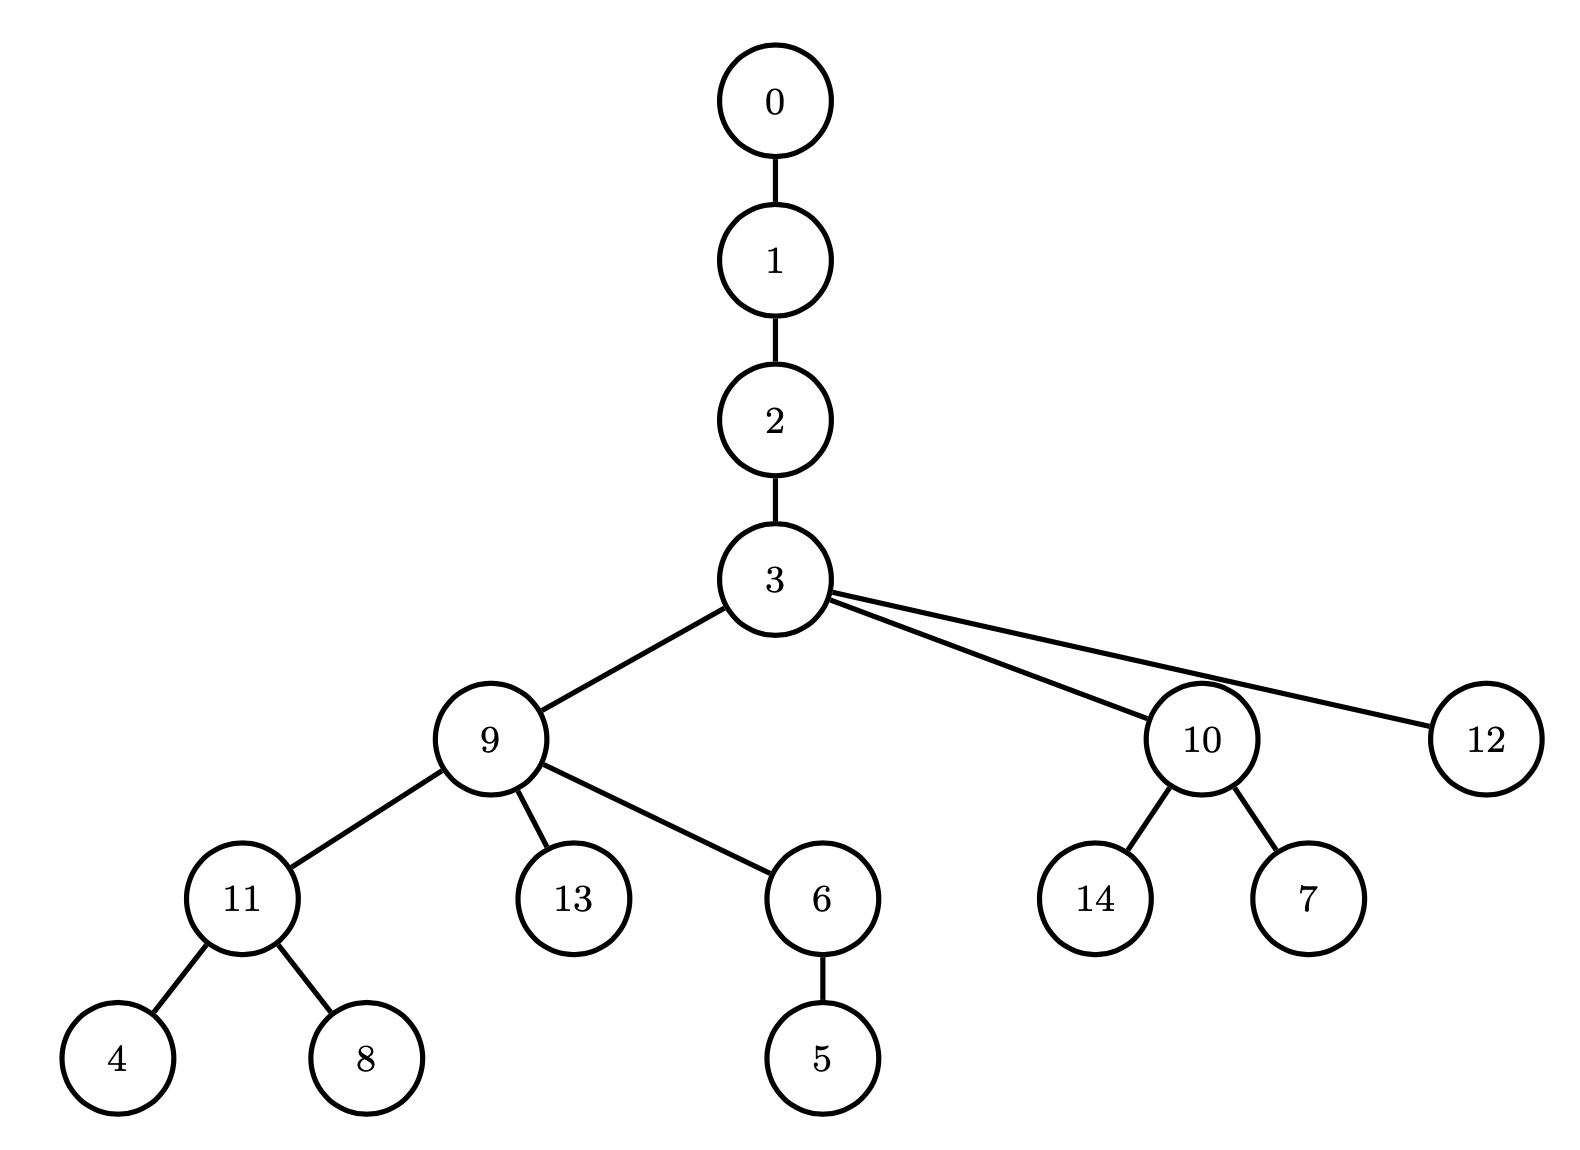
\includegraphics[width=11cm]{GRAPHICS/ORBITS/PGL_4_2_on_points}
$$
\caption{\label{fig:schreier:tree:PGL42}The Schreier tree for the action of $\PGL(4,2)$ on points of $\PG(3,2)$}
\end{figure}



\bigskip

Consider the wreath product acting on rank-one tensors from Section~\ref{sec:induced:actions}.
The following command sequence computes the orbits, 
exports the Schreier tree, and produces the drawing 
shown in Figure~\ref{fig:schreier:tree:wreath:tensor}.
\begin{figure}
$$

\includegraphics[width=11cm]{GRAPHICS/schreier_tree_wreath3_on_rank1_tensors}
$$
\caption{\label{fig:schreier:tree:wreath:tensor}The Schreier tree for the action on rank-one tensors}
\end{figure}
{\tt
\input GRAPHICS/THE_MAKEFILE/EXTRACTS/T3r1_orbits.tex
}

\bigskip


In the next example, we 
compute the orbits of 
the linear group $\PGL(4,2)$  on homogeneous polynomials of degree 3 in 4 variables: 
{\tt
\input GRAPHICS/THE_MAKEFILE/EXTRACTS/orbits_cubic_curves_q2.tex
}
This command computes the orbits of 
on all cubic forms in 4 variables, 
confirming the work of Dickson~\cite{Dickson15} 
and an enumerative result of Cooley~\cite{Cooley14}.


\bigskip

The next example computes orbits in an induced action. 
Induced actions have been described in Section~\ref{sec:induced:actions}. 
One group can have many actions. 
In particular, Orbiter can work with induced actions without changing the representation of the 
group elements. 
This has the advantage that the stabilizers are expressed in terms of the original action. 
To consider an example, 
suppose we want to consider the action of the stabilizer of a conic on the points of the plane 
(this continues an example from Section~\ref{sec:induced:actions}). 
The following command can be used:
{\tt
\input GRAPHICS/THE_MAKEFILE/EXTRACTS/PGGL_2_8_on_conic_orbits.tex
}
The output shown below. 
First, the orbits are listed. Then for each orbit, the stabilizer is 
shown, together with the generators in the action on the plane.
For the sake of space, some of the output has been shortened.
The three orbits correspond to the conic, 
the nucleus and the remaining points of the plane.
\begin{mdframed}[style=MyFrame]
\input GRAPHICS/LATEX/arc_Lunelli_Sce.tex
\end{mdframed}
A partially ordered set (poset) is a set together with a partial order. 
For instance, the set of subsets of a fixed set form an order structure 
with respect to set-inclusion.
The Hasse diagram is a diagram whose nodes represent the element. 
Nodes are arranged from top to bottom, 
and relations are indicated by lines. Transitivity is implied.
For instance, Figure~\ref{fig:subset:lattice:4} 
shows the power set lattice of a four-element subset.
\begin{figure}
$$
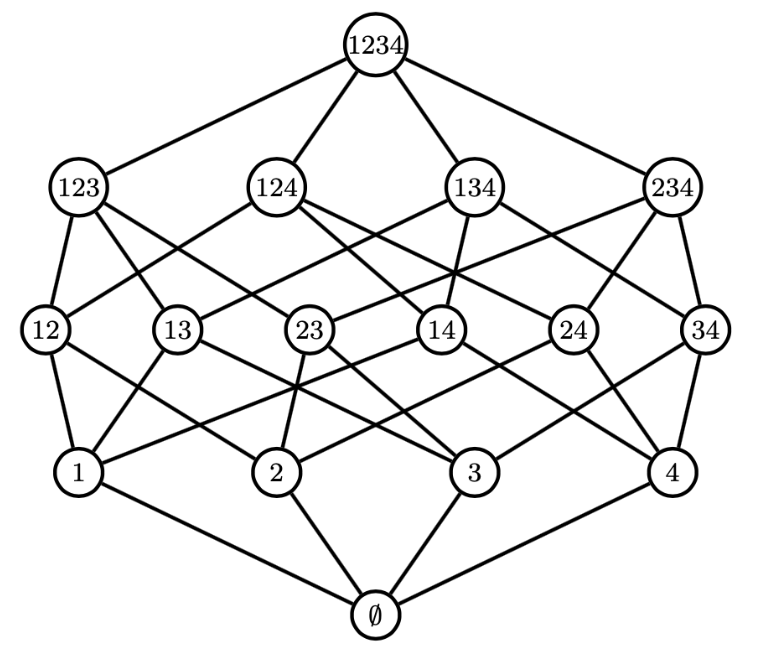
\includegraphics[width=9cm]{GRAPHICS/POSETS/subset_lattice_4}
$$
\caption{\label{fig:subset:lattice:4}Subset lattice of a 4-element set}
\end{figure}


\bigskip


Posets often come with group actions.
We say that a group $G$ acts on a poset $\cP$ if for all $x,y \in \cP$ and all $g \in G,$ 
$$
x \le y \Rightarrow xg \le yg.
$$
For background on poset actions, see Plesken~\cite{Plesken82}.
The orbits of $G$ on $\cP$ form another poset, the poset of orbits. 
The problem of classification of combinatorial objects can often be attacked by using group invariant relations. 
A layered poset can be decomposed into a series of relations. 
The layers allow to reduce the classification problem into small steps, 
namely from on layer to the next. This uses the incidence relation between adjacent layers.  
By iterating this method, one can form a poset of substructures, and the classification problem 
reduces to the problem of determining the orbits of the poset, 
which we will henceforth call the poset classification problem.
Many classification problem in Combinatorics reduce to poset classification problems. 


\bigskip


Orbiter uses the algorithm of Schmalz~\cite{Schmalz90} to perform poset classification.
Two versions are available: one for subset-type posets and one for subspace-type posets.
Figure~\ref{fig:subspace:lattice:V32} shows the subspace lattice of $V(3,2)=\bbF_2^3.$
\begin{figure}
$$
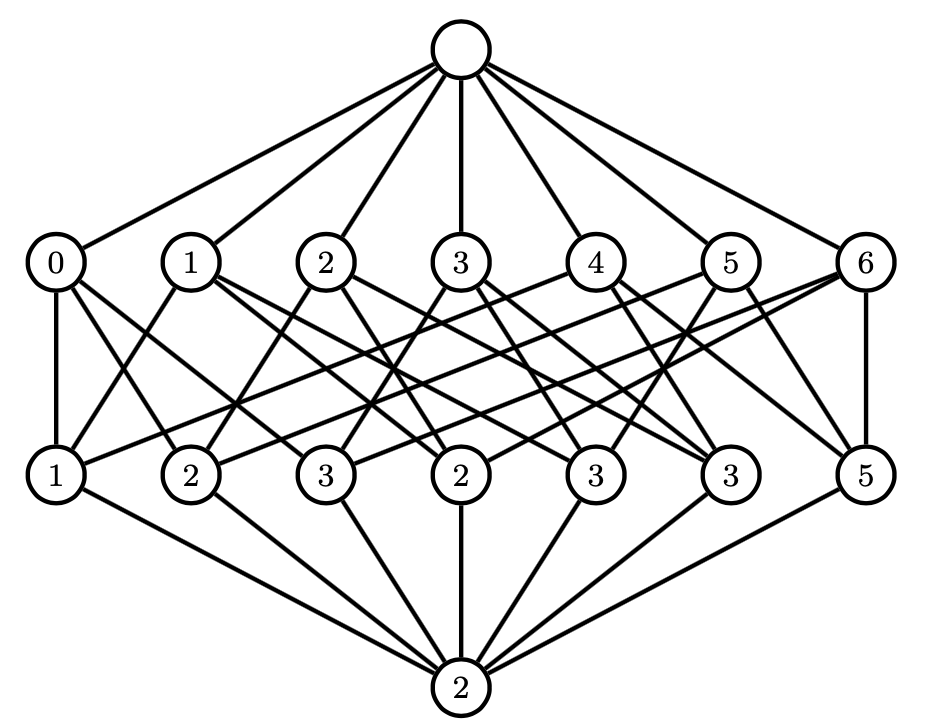
\includegraphics[width=9cm]{GRAPHICS/POSETS/V_3_2}
$$
\caption{\label{fig:subspace:lattice:V32}Subspace lattice of $V(3,2)$}
\end{figure}
The basis elements are listed, using the enumerator for 
elements on the projective geometry $\PG(2,2)$ 
explained in Section~\ref{sec:FPG}.


%A different algorithm is McKay~\cite{McKay98}.
%The way in which isomorph checking is handled in the two algorithms is very different. McKay relies on the notion of a 
%function that can compute a canonical form of an object. Such a function is difficult to provide and 
%in most cases relies on expensive backtracking. The Schmalz variant does not require such a function. 
%Instead, it can do isomorphism testing based on precomputed isomorphisms at lower levels in the poset. 
%By induction on the level, the complete orbit or posets is created one level at a time, in a breadth first manner. 
%On the other hand, McKay's algorithm proceeds depth-first, 
%and never needs to revisit a node that has been dealt with, 
%resulting in a smaller memory-footprint. 
%A more in-depth  comparison of the two algorithms has 
%yet to be done (See~\cite{Betten18a} for a brief attempt). 
%It seems that there are problems for which the Schmalz 
%variant has an advantage, for instance problems in the finite geometry. 
%On the other hand, McKay's algorithm performs very well on graphs. 
%The need for a canonical form algorithm somewhat limits the scope of problems for which McKay's algorithm 
%can be applied. At present, canonical form algorithms are available for very limited classes of objects. 
%McKay's software package Nauty~\cite{Nauty2020} deals with graphs. 
%Leon's software Part~\cite{Leon97} is devoted to codes and designs.
%On the other hand, the applications of Orbiter's classification algorithm are potentially unlimited. 
%At the moment, two types of 
%posets are avaliable. The poset can be a subposet of either the subset-lattice and the subspace-lattice. 
%The way that the poset is defined is by means of a test function. 
%This test function is provided by the user. The purpose of this test function is 
%to determine if an element in the corresponding lattice belongs to the poset or not. 


\bigskip


The commands shown in Table~\ref{tab:pc:options}
can be used to control the poset classification algorithm.
\begin{table}
\begin{center}
\begin{tabular}{|p{4cm}|p{3cm}|p{8cm}|}
\hline
Command & Arguments & Purpose \\
\hline
\hline
\verb'-problem_label' & str   & Use str as a prefix for files that are created. \\
\hline
\verb'-path' & $p$   & Use path $p$ for files that are created. \\
\hline
\verb'-depth' & $d$  & Set search depth to $d$. \\
\hline
\verb'-v' & $v$  & Set verbosity to $v$. Larger numbers mean more output. \\
\hline
\verb'-gv' & $v$  & Set verbosity for group theoretic operations to $v$. Larger numbers mean more output. \\
\hline
\verb'-recover' & fname  & Recover from the given file. \\
\hline
\verb'-lex' &   & Use the lexicographic ordering to speed up the search. \\
\hline
\verb'-w' &   & Save orbits at level $d$ only. \\
\hline
\verb'-W' &   & Save orbits at all levels. \\
\hline
\verb'-write_data_files' &   & Save data to files. \\
\hline
\verb'-t' &   & Write a file containing the search tree at level $d$.  \\
\hline
\verb'-T' &   & Write a file containing the search tree at all levels. \\
\hline
\verb'-draw_options' & options & Drawing options according to Table~\ref{tab:draw:options}. \\
\hline
\verb'-preferred_choice' & $n$ $a$ $b$ & 
At node $n$, choose $b$ instead of $a$ as orbit representative. This option can be repeated. \\
\hline
\verb'-clique_test' & graph  & 
Classify cliques in the given graph. \\
\hline
%\verb'-has_invariant_subset_for_root_node' & $S$  & 
%Set an invariant subset at the root node. \\
%\hline
%\verb'-do_group_extension_in_upstep' &  & 
%Use group extension in upstep. \\
%\hline
%\verb'-write_tree' &   & Write the poset of orbits as a tree file. \\
%\hline
%\verb'-find_node_by_' \verb'stabilizer_order' & $i$  & Find all nodes whose stabilizer has order $i$. \\
%\hline
%\verb'-draw_poset' &   & Produce a drawing of the poset of orbits. \\
%\hline
%\verb'-draw_full_poset' &   & Produce a drawing of the full poset with elements grouped by orbits. \\
%\hline
%\verb'-plesken' &   & Compute Plesken matrices Asup and Ainf. \\
%\hline
%\verb'-print_data_' \verb'structure' &   & Print the data structure. \\
%\hline
%\verb'-list' &   & List orbits at level $d$. \\
%\hline
\end{tabular}
\end{center}
\caption{\label{tab:pc:options}Options to control the poset classification algorithm}
\end{table}
%\begin{table}
%\begin{center}
%\begin{tabular}{|p{4cm}|p{3cm}|p{8cm}|}
%\hline
%Command & Arguments & Purpose \\
%\hline
%\hline
%\verb'-list_all' &   & List orbits at all levels. \\
%\hline
%\verb'-table_of_nodes' &   & Produce a spreadsheet of all orbits. \\
%\hline
%\verb'-make_relations_' \verb'with_flag_orbits' &   & Produce a bitmap drawing of the neighboring relations in the poset with flag orbits. \\
%\hline
%\verb'-Kramer_Mesner_' \verb'matrix' &  $t$ $k$ & Compute the Kramer-Mesner matrix $M_{t,k}$. \\
%\hline
%\verb'-level_summary_csv' &   & Write a summary of number of orbits at each level to a csv file. \\
%\hline
%\verb'-orbit_reps_csv' &   & Write orbit representatives to a csv file. \\
%\hline
%\verb'-report' .. \verb'-end' &   & Produce a latex report. Requires \verb'-orbiter_path' option from Section~\ref{sec:session}. \\
%\hline
%\verb'-node_label_' \verb'is_group_order' &   & When drawing the poset of orbits, display the group order in the orbit nodes. \\
%\hline
%\verb'-node_label_' \verb'is_element' &   & When drawing the poset of orbits, display the element rank in the orbit nodes. \\
%\hline
%\verb'-show_orbit_' \verb'decomposition' &   & Show the orbits of the stabilizers. \\
%\hline
%\verb'-show_stab' &   & Show the stabilizers. \\
%\hline
%\verb'-save_stab' &   & Save the stabilizer generators. \\
%\hline
%\verb'-show_whole_orbits' &   & Show the whole orbits. \\
%\hline
%\verb'-recognize' & $L$  & Recognize the given object in the classified list and compute a transporter that maps the given object to the canonical form. Here, $L$ must be a list of integers (comma separated and enclosed in double quotes) encoding an object. This option can be repeated. \\
%\hline
%\verb'-export_' \verb'schreier_trees' &   & Export all Schreier trees. \\
%\hline
%\verb'-draw_' \verb'schreier_trees' &  args  & Draw all Schreier trees. \\
%\hline
%\end{tabular}
%\end{center}
%\caption{\label{tab:pc:options2}Options to control the poset classification algorithm (Part 2)}
%\end{table}
By default, Orbiter will choose the lexiographically least orbit representatives. 
It is possible to direct Orbiter to choose different orbit representatives. 
To this end, the nodes in the orbit tree are labeled. 
The node number is the zero-based number of a given node in the tree, 
using the breadth first ordering. 

\bigskip


Suppose that orbiter chooses element $a$ at node $n.$ 
Suppose we are interested in choosing element $b$ instead. 
The command 
$$
\verb'-preferred_choice' \; n \; a \; b
$$
can be used to force Orbiter to choose $b$ instead of $a$ at node $n$.

The lattice of subsets of a set $X$ is $\frakP(X),$ the set of all subsets of $X$, ordered with respect to inclusion. 
%For instance, Figure~\ref{fig:subsets4} shows the lattice of subsets of a 4-element set.
%\begin{figure}
%$$
%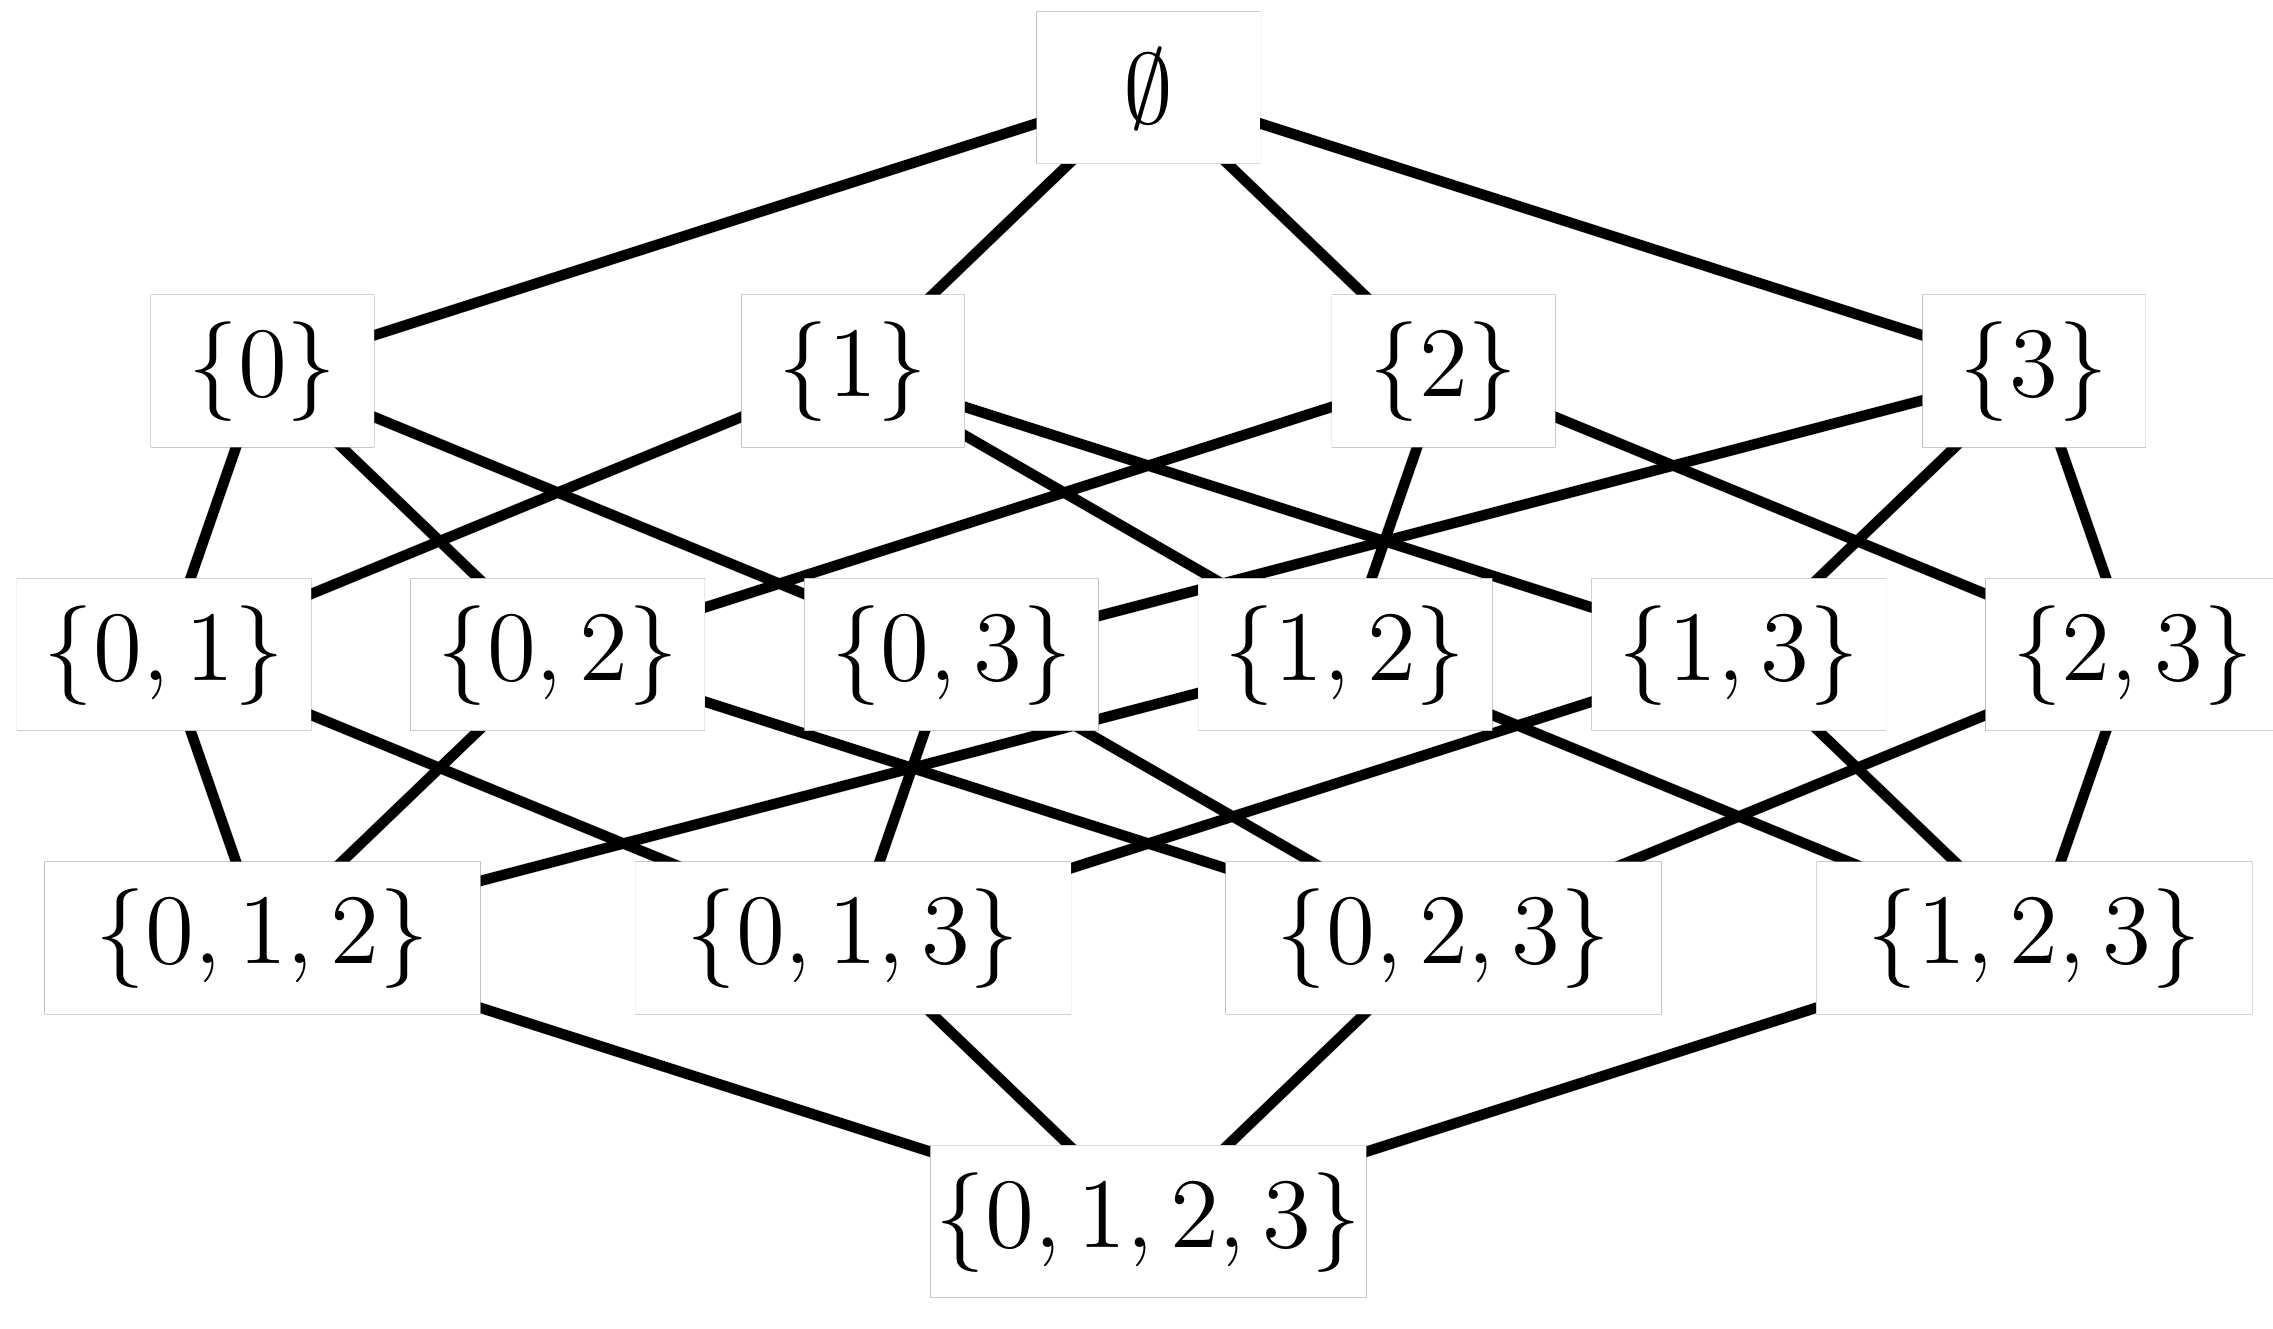
\includegraphics[width=10cm]{GRAPHICS/POSETS/poset_of_subsets4_modified}
%$$
%\caption{\label{fig:subsets4}The lattice of subsets of a 4-element set}
%\end{figure}
Assume that a group $G$ acts on $X$, and hence on the lattice by means of the induced action on subsets. 
The orbits of $G$ on subsets form a new poset, the poset of orbits. 
Poset classification is the process of computing the poset of orbits. 
Orbiter has an algorithm to perform poset classification. 
In many cases, we are not interested in the full lattice of subsets $\frakP(X)$ 
but rather in a subposet of it.
We require that the subposet is closed under the group action and that the following property holds:
$$
x, y \in \frakP(X) \; \mbox{and} \; x \le y \;  \Rightarrow \; \Big( y \in \cP \rightarrow x \in \cP \Big).
$$
The join of two subsets in the poset may or may not belong to the poset.
Let us consider the action of the Singer cycle on $\PG(3,2).$
The following command computes the orbits of the group $G$ generated by a Singer cycle in $\PG(3,2)$:
{\tt
\input GRAPHICS/THE_MAKEFILE/EXTRACTS/PGL_3_2_singer.tex
}

\bigskip

The next command computes the orbits of the projective group $\PGL(4,2)$ 
acting on all subsets of $\PG(3,2)$:
{\tt
\input GRAPHICS/THE_MAKEFILE/EXTRACTS/PG_3_2_subsets.tex
}
A drawing of the poset of orbits as in Figure~\ref{PGL42:on:subsets} is produced.
\begin{figure}
$$
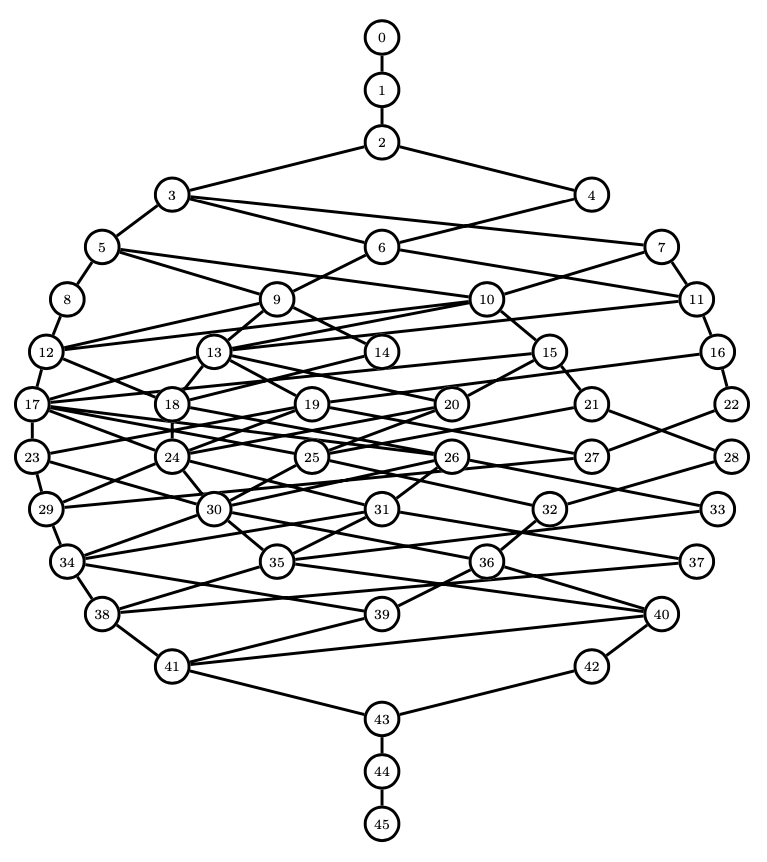
\includegraphics[width=11cm]{GRAPHICS/PGL_4_2/PGL_4_2_orbits_on_subsets}
$$
\caption{\label{PGL42:on:subsets}The orbits of $\PGL(4,2)$ on subsets}
\end{figure}


\bigskip

Orbiter can compute orbits of groups acting in various different actions. 
The following example computes the orbits of $\PGL(3,2)$ 
on the subsets of lines of $\PG(2,2).$
{\tt
\input GRAPHICS/THE_MAKEFILE/EXTRACTS/PGL_3_2_on_lines.tex
}


\bigskip

The following example computes the orbits of $\PGO(5,2)$ 
on the power set lattice of points of $Q(4,2)$:
{\tt
\input GRAPHICS/THE_MAKEFILE/EXTRACTS/PGO_5_2_on_subsets.tex
}
The poset of orbits is shown in Figure~\ref{fig:PGO:5:2:orbits}.
\begin{figure}
$$
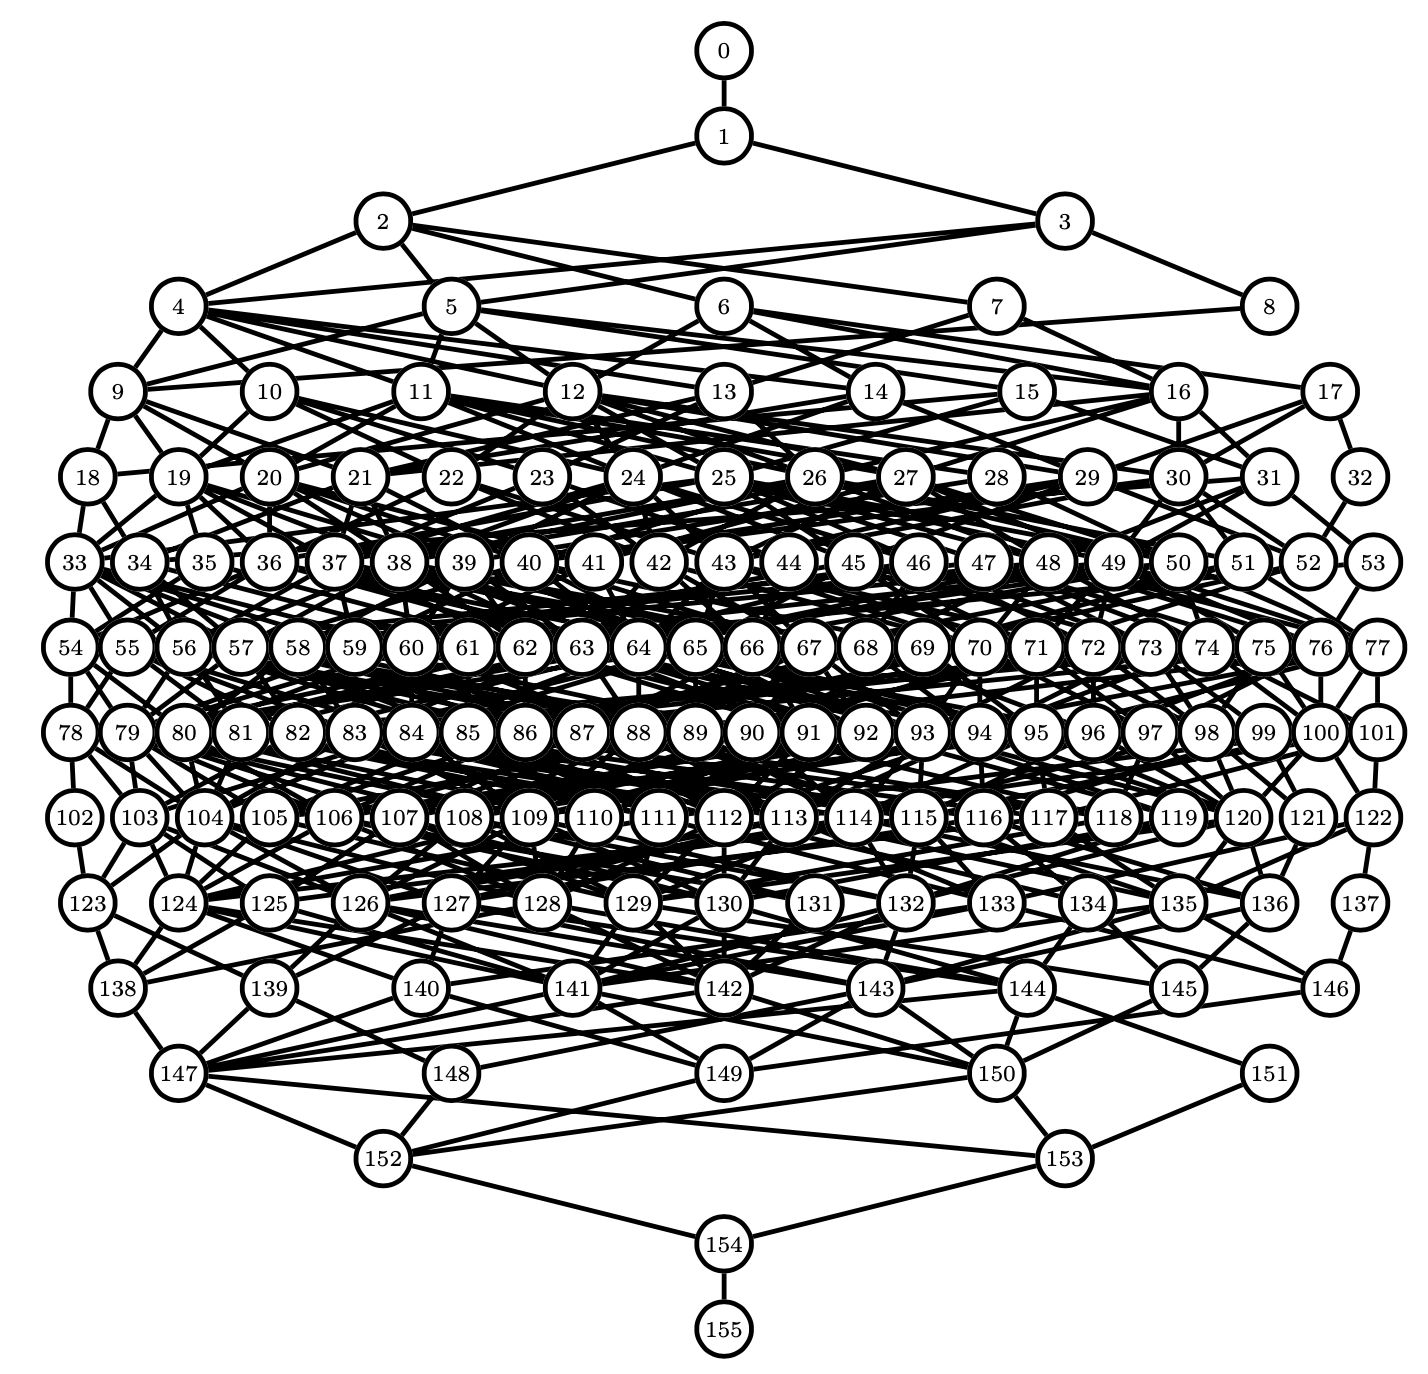
\includegraphics[width=15cm]{GRAPHICS/PGO_5_2/poset_orbits}
$$
\caption{\label{fig:PGO:5:2:orbits}Orbits of $\PGO(5,2)$ on the poset of subsets of $Q(4,2)$}
\end{figure}
Orbiter can compute the orbits of a group on 
the lattice of subspaces of a finite vector space.

\bigskip


The orthogonal group is the stabilizer of a non-degenerate quadric.  
Suppose we want to classify the subspaces in $\PG(3,2)$ under 
the action of the orthogonal group. 
In $\PG(3,2)$ there are two distinct nondegenerate quadrics, 
$Q^+(3,2)$ and $Q^-(3,2).$ 
The $Q^+(3,2)$ quadric is a finite version of the quadric given by the equation 
$$
x_0x_1 + x_2x_3 = 0,
$$
and depicted over the real numbers in Figure~\ref{fig:H3}.
\begin{figure}
$$
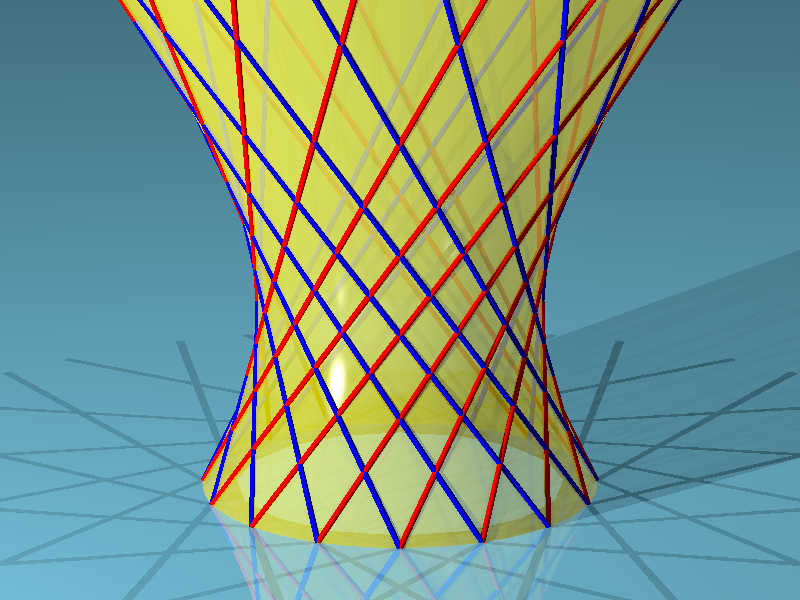
\includegraphics[width=9cm]{GRAPHICS/POVRAY/hyperboloid}
$$
\caption{\label{fig:H3}The hyperbolic quadric in affine space $\bbR^3$}
\end{figure}
$\PG(3, 2)$ has 15 points:\\
\begin{multicols}{4}
$P_{0}=( 1, 0, 0, 0 )$\\
$P_{1}=( 0, 1, 0, 0 )$\\
$P_{2}=( 0, 0, 1, 0 )$\\
$P_{3}=( 0, 0, 0, 1 )$\\
$P_{4}=( 1, 1, 1, 1 )$\\
$P_{5}=( 1, 1, 0, 0 )$\\
$P_{6}=( 1, 0, 1, 0 )$\\
$P_{7}=( 0, 1, 1, 0 )$\\
$P_{8}=( 1, 1, 1, 0 )$\\
$P_{9}=( 1, 0, 0, 1 )$\\
$P_{10}=( 0, 1, 0, 1 )$\\
$P_{11}=( 1, 1, 0, 1 )$\\
$P_{12}=( 0, 0, 1, 1 )$\\
$P_{13}=( 1, 0, 1, 1 )$\\
$P_{14}=( 0, 1, 1, 1 )$\\
\end{multicols}
The $Q^+(3,2)$ quadric given by the equation above consists of 
the nine points
$$
P_0, P_1, P_2, P_3, P_4, P_6,P_7,P_9,P_{10}.
$$
The quadric is stabilized by the group $\PGO^+(4,2)$ of order 72.
The command
{\tt
\input GRAPHICS/THE_MAKEFILE/EXTRACTS/subspaces_Op_4_2.tex
}
produces a classification of all 
subspaces of $\PG(3,2)$ under $\PGO^+(4,2).$ 
The option \verb'-draw_poset'
creates a Hasse diagram of the classification as shown in Figure~\ref{fig:H32}.
\begin{figure}
$$
%
\includegraphics[width=6cm]{GRAPHICS/O4_2}
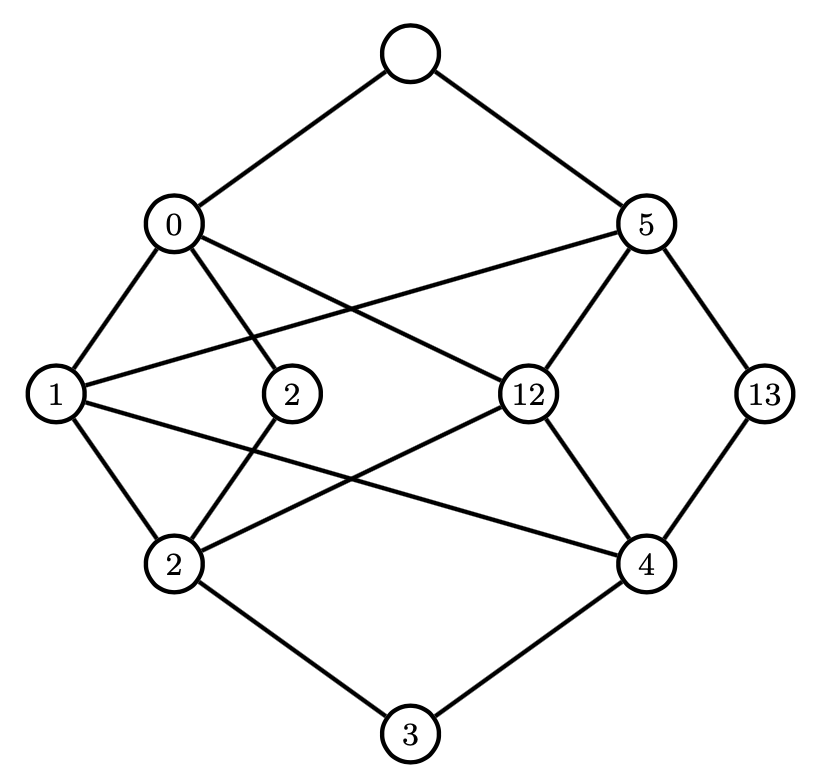
\includegraphics[width=7cm]{GRAPHICS/POSETS/Op_4_3_element}
$$
\caption{\label{fig:H32}Hasse-diagram for the orbits of the 
orthogonal group $\PGO^+(4,2)$ on subspaces of $\PG(3,2)$}
\end{figure}
The nodes show the ranks of points in $\PG(3,2)$ as described in Section~\ref{sec:FPG}.
Orbiter can compute the orbits of a group on set-partitions. 
The set-partition needs to have three parts of equal size.

\bigskip




The command
{\tt
\input GRAPHICS/THE_MAKEFILE/EXTRACTS/C6_on_partition.tex
}
computes the orbits of the cyclic group $C_6$ on set-partitions of type $2+2+2$.
There are 15 set-partitions, and they fall into 5 orbits, with stabilizer orders
$$
3,1,2,2,6.
$$
The orbit count gives 
$$
6\Big(
\frac{1}{3}+
\frac{1}{1}+
\frac{1}{2}+
\frac{1}{2}+
\frac{1}{6}
\Big)
=15.
$$

\bigskip


The command
{\tt
\input GRAPHICS/THE_MAKEFILE/EXTRACTS/PGL_2_17_on_partition.tex
}
computes the orbits of the  group $\PGL(2,17)$ on set-partitions of type $6+6+6$.
The number of set-partitions is 
$$
\frac{{18 \choose 6} \cdot {12 \choose 6}}{3!}
=2858856
$$
There are 720 orbits. The orbit stabilizer statistic is 
$$
( 1^{480}, 2^{184}, 3^{11}, 4^{20}, 6^{15}, 8, 12^6, 18, 24, 36 ).
$$
The orbit-stabilizer count confirms that
$$
4896
\Big(
\frac{480}{1}+
\frac{184}{2}+
\frac{11}{3}+
\frac{20}{4}+
\frac{15}{6}+
\frac{1}{8}+
\frac{6}{12}+
\frac{1}{18}+
\frac{1}{24}+
\frac{1}{36}+
\Big)
=2858856.
$$
In $\PG(n,q)$, an arc is a set of points, no $n+1$ in a hyperplane.
A cap is  set of points, no three collinear.
Here, we restrict our attention to arcs in $\PG(2,q).$  
Arcs in higher dimensional  projective spaces 
are equivalent to MDS codes and will be treated in Section~\ref{sec:coding}.
Our main examples will be the construction of the Lunelli-Sce hyperoval in $\PG(2,16)$ 
(cf.~\cite{LunelliSce58})
and the Pellegrino cap in $\AG(4,3).$ 
The uniqueness of this cap was proven by Hill~\cite{Hill83}.

\bigskip


A $(k,d)$-arc in a projective plane $\pi$ 
is a set $S$ of $k$ points such that very line intersects $S$ in at most $d$ 
points. Arcs are related to linear codes and other structures. Two arcs $S_1$ and $S_2$ 
are equivalent if there is a projectivity $\Phi$ such that $\Phi(A) = B.$ The problem of classifying arcs 
is the problem of determining the orbits of the projectivity group on arcs. At times, 
we consider the larger group of collineations. In that case, the problem of classifying arcs is the 
problem of determining the orbits of the collineation group on arcs. 
Orbiter can solve such classification problems, at least for small parameter cases. 
Table~\ref{tab:arcs} list the commands available to classify arcs.
\begin{table}
\begin{center}
\begin{tabular}{|p{4cm}|p{3cm}|p{8cm}|}
\hline
Command  & Arguments & Purpose \\
\hline
\hline
\verb'-q' & $q$ & Specify the size of the field $\bbF_q$. \\
\hline
\verb'-d' & $d$ & Require that no more than $d$ points lie on a line. \\
\hline
\verb'-n' & $n$ & The size of the matrix group. \\
\hline
\verb'-target_size' & $t$ & Specify the size of the arc to be $t$. \\
\hline
\verb'-conic_test' & & Require that no $6$ points of the arc lie on a conic. \\
\hline
\verb'-affine' & & Classify arcs in the affine geometry, assuming that $x_0 = 0$ is the hyperplane at infinity. The condition that no more that $d$ point lie on a line applies to affine lines only. \\
\hline
\verb'-no_arc_testing' & & Do not test the at most $d$ points per line condition. \\
\hline
\verb'-forbidden_' \verb'point_set' & set & The arc must not contain any of the given points. \\
\hline
\end{tabular}
\end{center}
\caption{\label{tab:arcs}Commands for Classifying Arcs}
\end{table}
Here is an example. A hyperoval in a plane $\PG(2,2^e)$ is a $(2^e + 2,2)$-arc. 
It is interesting to classify the hyperovals up to collineation equivalence under the group $\PGGL(3,2^e).$ 
The command 
{\tt
\input GRAPHICS/THE_MAKEFILE/EXTRACTS/subspaces_Op_4_2.tex
}
performs the classification of hyperovals in $\PG(2,16).$ 
There are exactly two hyperovals in this plane. 
Orbiter also finds the stabilizers of these arcs. 
They have orders $16320$ and $144,$ respectively.
The two hyperovals are the regular hyperoval and the Lunelli-Sce hyperoval. 
Here is the relevant output from the Orbiter report 
(in the output, the Lunelli-Sce hyperoval is orbit 0, and the 
regular hyperoval is orbit 1):
\begin{mdframed}[style=MyFrame]
\input GRAPHICS/LATEX/arc_Lunelli_Sce.tex
\end{mdframed}


\bigskip



\bigskip

In the theory of cubic surfaces, we are interested in non-conical arcs. 
These are arcs which do not lie on a conic.
The following example demonstrates how this can be done in Orbiter:
{\tt
\input GRAPHICS/THE_MAKEFILE/EXTRACTS/nc_arcs_16.tex
}
Cubic surfaces are associated with arcs of size 6 
(in a many-to-one relationship when considering isomorphism classes).
The number of Eckardt points of the surface can be recovered from properties of the arc.
For this reason, it is interesting to classify arcs so that the associated 
cubic surface has a fixed number of Eckardt points.
The following command shows how to create all arcs associated 
with cubic surfaces with 13 Eckardt points over the field $\bbF_{32}$:
{\tt
\input GRAPHICS/THE_MAKEFILE/EXTRACTS/nc_arcs_32_E13.tex
}

Orbiter can classify cubic curves in $\PG(2,q)$. 
To this end, the $(9,3)$-arcs in $\PG(2,q)$ are classified first.
From this classification, the classification of curves is computed.
This classification only works for arcs which contain a $(9,3)$ arc. 
For very small fields, this is not always the case. 

Here is an example. The command  
{\tt
\input GRAPHICS/THE_MAKEFILE/EXTRACTS/cubic_curves_PG_2_8.tex
}
classifies the cubic curves in $\PG(2,8).$
\section{Creation}
\label{sec:cubicsurfaces:creation}

\input C07/sec_1.tex


\bigskip

\clearpage


\section{Quartic Curves}
\label{sec:cubic:surfaces:quartic:curves}

\input C07/sec_2.tex


\bigskip

\clearpage


\section{Classification}
\label{sec:cubicsurfaces:classification}

\input C07/sec_3.tex


\bigskip

\clearpage


\section{Isomorphism Testing and Recognition}
\label{sec:cubicsurfaces:iso:rec}

\input C07/sec_4.tex


\bigskip

\clearpage


\section{Dickson Surfaces}
\label{sec:cubicsurfaces:Dickson}

\input C07/sec_5.tex


\bigskip

\clearpage


\section{ATLAS and Tables}
\label{sec:cubicsurfaces:ATLAS}

\input C07/sec_6.tex


\bigskip

\clearpage
Orbiter can create, classify and investigate cubic surfaces over small finite fields. 
In this section, we describe ways in which surfaces can be created. 
The following sections will be about classification and investigation.

\bigskip

Orbiter contains a built-in catalogue of cubic surfaces with 27 
lines for small finite fields $\bbF_q.$ 
The surfaces in the catalogue all come with their automorphism group.
It is also possible to create surfaces from known families, 
or to create surfaces from associated objects like 6-arcs. 
Some of these constructions only create the surface, 
not the automorphism group.

\bigskip

Tables~\ref{tab:createsurface:one}-\ref{tab:createsurface:three} 
summarize the Orbiter commands that can be used
to create cubic surfaces. 
The commands are applied to a projective space object, 
which must be created first.
Not all of the surfaces created may have 27 lines, 
and some of the constructions may yield degenerate surfaces. 
\begin{table}
\begin{center}
\begin{tabular}{|p{4cm}|p{3cm}|p{7cm}|}
\hline
Command & Arguments & Purpose \\
\hline
\hline
\verb'-space' &  P & Specify the 3-dimensional projective space P $=\PG(3,q)$. \\
\hline
\verb'-label_txt' & label & Override the ascii label of the curve. \\
\hline
\verb'-label_tex' & label & Override the latex label of the curve. \\
\hline
\verb'-label_for_summary' & label & Override the ascii label of the curve, to be used in summary commands. \\
\hline
\verb'-catalogue' & $i$   & 
Create the $i$-th surface in the Orbiter catalogue. 
Here, $i$ is an index variable used to index all surfaces in $\PG(3,q)$. 
The index $i$ is zero-based. 
The automorphism group is created as well. \\
\hline
\verb'-by_coefficients'& list-of-coeff-pairs  & 
Create a surface from a list of coefficient-monomial pairs. 
The automorphism group is not created. \\
\hline
\verb'-by_rank'& rank $q_0$  & 
Create a surface from the numerical rank of the equation over the 
subfield $\bbF_{q_0}$. 
Here, we think of the equation as a 
point in $\PG(19,q_0)$ and use the Orbiter point rank. \\
\hline
\verb'-family_Eckardt' & $a$ $b$  & 
Create the Eckardt surface with parameters $(a,b)$ 
as in see~\cite{BettenKaraoglu19a} 
(where it is called the Hilbert, Cohn-Vossen surface). 
The equation is 
$X_3^3-b^2(X_0^2+X_1^2+X_2^2)X_3+ 
\frac{b^3}{a}(a^2+1)X_0X_1X_2 = 0.$ 
The automorphism group is created as well. \\
\hline
\end{tabular}
\end{center}
\caption{\label{tab:createsurface:one}Commands to create a cubic surface (Part 1)}
\end{table}
\begin{table}
\begin{center}
\begin{tabular}{|p{4cm}|p{3cm}|p{7cm}|}
\hline
Command & Arguments & Purpose \\
\hline
\hline
\verb'-family_G13' & $a$   & 
Create a member of the $G_{13}$ family with parameter $a$. 
The surface has 13 Eckardt points. \\
\hline
\verb'-family_F13' & $a$   & 
Create a member of the $F_{13}$ family with parameter $a$. 
The surface has 13 Eckardt points. \\
\hline
\verb'-family_bes' & $a$ $c$  & 
Create a member of the ``bes''-family with parameter $a$. 
The surface has 5 Eckardt points. \\
\hline
\verb'-family_general_' \verb'abcd' & $a$ $b$ $c$ $d$  & 
Create a member of the general family with parameters $a,b,c,d$. \\
\hline
\verb'-arc_lifting' & $A$    & 
Create the surface associated with the arc 
$A=a_1,\ldots,a_6$ in $\PG(2,q)$ by means of the Clebsch map. 
Each of the $a_i$ is the rank of a point in $\PG(2,q).$ 
Use the trihedral pair algorithm. 
Here, $A$ is a comma-separated string containing the numerical 
ranks of the $P_i$ in $\PG(2,q).$\\
\hline
\verb'-arc_lifting_' \verb'with_two_lines' & $A$  $L$  & 
Create the surface associated with the arc 
$A=a_1,\ldots,a_6$ in $\PG(2,q)$ by means of the Clebsch map, 
defined by the lines $\ell_1$ and $\ell_2$ whose ranks are given in $L$.
If both of the lines are given as 0, the program will pick a 
suitable set of lines automatically.\\ 
\hline
\end{tabular}
\end{center}
\caption{\label{tab:createsurface:two}Commands to create a cubic surface (Part 2)}
\end{table}
\begin{table}
\begin{center}
\begin{tabular}{|p{4cm}|p{3cm}|p{7cm}|}
\hline
Command & Arguments & Purpose \\
\hline
\hline
\verb'-Cayley_form' & $k$ $l$ $m$ $n$   & 
Create the surface from Cayley's normal form, using the parameters $k,l,m,n.$\\
\hline
\verb'-by_equation' &    & 
Create the surface from an equation.\\
\hline
\verb'-by_double_six' &  $D$  & 
Create the surface from a double six $D$.\\
\hline
\verb'-by_skew_hexagon' &  label label  & 
Create the surface from a skew hexagon.\\
\hline
\verb'-select_double_six' &  $L$   & 
Relabel the lines by choosing the 12 lines in $L$ as new double six. 
The entries in $L$ are line indices with respect to the old double six. 
They are integers in the interval $[0,26].$ 
This command can be repeated. 
In each application, the double six refers to the previous labeling. \\
\hline
\verb'-override_group' & descr & Override the automorphism group of the surface by the given group. \\
\hline
\verb'-transform' & elt & Apply the transformation given by the group element. \\
\hline
\verb'-transform_inverse' & elt & Apply the inverse transformation given by the group element. \\
\hline
\end{tabular}
\end{center}
\caption{\label{tab:createsurface:three}Commands to create a cubic surface (Part 3)}
\end{table}


Table~\ref{tab:cubic:surface:activities} lists activities for a cubic surface object.
\begin{table}
\begin{center}
\begin{tabular}{|p{4cm}|p{3cm}|p{8cm}|}
\hline
Command & Arguments & Purpose \\
\hline
\hline
\verb'-report' & & Produce a latex report about the cubic surface. \\
\hline
%\verb'-report_with_group' & & Produce a latex report about the cubic surface. The report include group theoretic information about the automorphism group and the action on the surface. \\
%\hline
\verb'-export_something' & type & Exports data about the surface to a file. The type of data to be exported must be specified according to Table~\ref{tab:cubic:surface:export}. \\
\hline
\verb'-all_quartic_curves' & & Creates all quartic curves with 28 bitangents from the surface by projecting along the tangent cone of a point not on any line.   \\
\hline
\verb'-export_all_' \verb'quartic_curves' & & Creates all quartic curves with 28 bitangents from the surface by projecting along the tangent cone of a point not on any line. Writes a csv file with the curves that have been created.  \\
\hline
%\verb'-export_' \verb'tritangent_planes' & & Writes a file containing all tritangent planes of the surface.\\
%\hline
\end{tabular}
\end{center}
\caption{\label{tab:cubic:surface:activities}Activities related to cubic surfaces}
\end{table}

\begin{table}
\begin{center}
\begin{tabular}{|p{4cm}|p{8cm}|}
\hline
Command  & Purpose \\
\hline
\hline
\verb'points' & The points on the surface. \\
\hline
\verb'points_off' & The points off the surface. \\
\hline
\verb'Eckardt_points' & The Eckardt points of the surface. \\
\hline
\verb'double_points' & The double points of the surface. \\
\hline
\verb'single_points' & The single points of the surface. \\
\hline
\verb'zero_points' & The zero points of the surface. A point is a zero point if it does not lie on any line.\\
\hline
\verb'singular_points' & The singular points of the surface. \\
\hline
\verb'lines' & The set of lines of the surface. \\
\hline
\verb'tritangent_planes' & The set of tritangent planes of the surface. \\
\hline
\verb'Hesse_planes' & The set of Hesse planes of the surface. \\
\hline
\end{tabular}
\end{center}
\caption{\label{tab:cubic:surface:export}Options for exporting data}
\end{table}


Let us look at some examples. 
The next command creates the unique surface with 27 lines 
over the field $\bbF_4.$ 
It is the Hirschfeld surface. 
In this command, the surface is pulled from Orbiter's built-in catalogue of cubic surfaces. 
The surface has Orbiter Catalogue Number (OCN) equal to 0.
{\tt
\input GRAPHICS/THE_MAKEFILE/EXTRACTS/surface_4_0.tex
}
A report is created and several data elements 
of the surface are exported: the set of points on and off the surface, 
the set of lines, and the set of Hesse planes.

\bigskip


In the following command, the surface over $\bbF_7$ with catalogue number 0 is created, a reportis written, 
and the set of lines is exported:
{\tt
\input GRAPHICS/THE_MAKEFILE/EXTRACTS/surface_7_0.tex
}

\bigskip



Another way of creating surfaces is as members of known infinite families.
For instance, 
{\tt
\input GRAPHICS/THE_MAKEFILE/EXTRACTS/surface_eckardt_13_4_12.tex
}
creates the member of the Eckardt family  
described in~\cite{BettenKaraoglu19a} 
with parameters $(a,b) = (4,12)$ over the field $\bbF_{13}.$

\bigskip



It is often desired to produce a nice equation of a cubic surface. This can be done by applying 
coordinate changes. In the following example, a ``nice'' equation for the cubic surface over $\bbF_{16}$
with catalogue number 0 is produced:
{\tt
\input GRAPHICS/THE_MAKEFILE/EXTRACTS/surface_16_0.tex
}


\bigskip



Let us try the 4-parameter normal form of cubic surfaces with parameters $a,b,c,d.$ 
The formula can be encoded in a makefile variable:
{\tt
\input GRAPHICS/THE_MAKEFILE/EXTRACTS/F_abcd_eqn_no_exponents.tex
}
The following command parses the formula and creates the surface with $(a,b,c,d)=(4,2,2,4)$ over $\bbF_7$:
{\tt
\input GRAPHICS/THE_MAKEFILE/EXTRACTS/surface_F_abcd_q7.tex
}


\bigskip

It is possible to recreate the surface with the generators for the automorphism group.
The following command creates two reports about the surface. 
One with and one without information about the group action.
{\tt
\input GRAPHICS/THE_MAKEFILE/EXTRACTS/surface_F_alpha_beta_gamma_delta_q7_override_group.tex
}



Cubic surfaces with 27 lines are associated with 
quartic curves with 28 bitangents (see~\cite{Hirschfeld82}), 
which in turn are associated with del Pezzo surfaces. 
Orbiter can classify quartic curves based on a known classification of cubic surfaces.
Orbiter also has a catalogue of quartic curves for small field sizes.

\bigskip


Table~\ref{tab:quartic:curves:create} lists options to create a quartic curve object.
\begin{table}
\begin{center}
\begin{tabular}{|p{4cm}|p{3cm}|p{8cm}|}
\hline
Command & Arguments & Purpose \\
\hline
\hline
\verb'-space' & P & Specify the 2-dimensional projective space P $=\PG(2,q)$. \\
\hline
\verb'-label_txt' & label & Override the ascii label of the curve. \\
\hline
\verb'-label_tex' & label & Override the latex label of the curve. \\
\hline
\verb'-label_for_summary' & label & Override the ascii label of the curve, to be used in summary commands. \\
\hline
\verb'-catalogue' & OCN & Create the quartic curve from the Orbiter catalogue with the given Orbiter catalogue number.\\
\hline
\verb'-by_coefficients' & coeffs & Create a quartic curve given the coefficients of the equation. \\
\hline
\verb'-by_equation' & eqn & Create a quartic curve from an equation. \\
\hline
\verb'-from_cubic_surface' & $S$ $i$ & Create the quartic curve from $i$th orbit of the automorphism group of the surface $S$ on points not on lines ($i$ is zero based). \\
\hline
\verb'-override_group' & descr & Override the automorphism group of the curve by the given group. \\
\hline
\verb'-transform' & elt & Apply the transformation given by the group element. \\
\hline
\verb'-transform_inverse' & elt & Apply the inverse transformation given by the group element. \\
\hline
\end{tabular}
\end{center}
\caption{\label{tab:quartic:curves:create}Options to create a quartic curve}
\end{table}


\bigskip
Table~\ref{tab:quartic:curves:activities} lists activities for a quartic curve object.
\begin{table}
\begin{center}
\begin{tabular}{|p{4cm}|p{3cm}|p{8cm}|}
\hline
Command & Arguments & Purpose \\
\hline
\hline
\verb'-report' & & Produce a latex report about the curve. \\
\hline
\verb'-export_something' & type & Exports data of the quartic curve to a file. The type of data to be exported must be specified according to Table~\ref{tab:quartic:curve:export}. \\
\hline
\verb'-create_surface' & & Create a cubic surface from the curve. \\
\hline
\verb'-extract_orbit_' \verb'on_bitangents_' \verb'by_length' & $l$ & Extract the bitangents in the unique orbit of length $l$. If there is no orbit of length $l$, or if there are multiple orbits of length $l$, an error is raised. \\
\hline
\verb'-extract_specific' \verb'_orbit_on_' \verb'bitangents_' \verb'by_length' & $l$ $i$ & Extract the $i$th orbit on bitangents of length $l$. \\
\hline
\verb'-extract_specific' \verb'_orbit_on_' \verb'kovalevski_points_' \verb'by_length' & $l$ $i$ & Extract the $i$th orbit on Kovalevski points of length $l$. \\
\hline
\end{tabular}
\end{center}
\caption{\label{tab:quartic:curves:activities}Activities related to quartic curves}
\end{table}


\begin{table}
\begin{center}
\begin{tabular}{|p{4cm}|p{8cm}|}
\hline
Command  & Purpose \\
\hline
\hline
\verb'points' & The points on the quartic curve. \\
\hline
\verb'equation' & The equation of the quartic curves as a coefficient vector of length 15. \\
\hline
\verb'bitangents' & The 28 bitangents. \\
\hline
\verb'Kovalevski_points' & The Kovalevski points (points off the curve where 4 bitangents meet). \\
\hline
\verb'singular_points' & The singular points of the curve. \\
\hline
\end{tabular}
\end{center}
\caption{\label{tab:quartic:curve:export}Options for exporting data}
\end{table}




\bigskip


Suppose we want to study the (unique) quartic curve for $q=9$.
The follwing command creates the curve whose catalogue number is 0, and produces a report:
{\tt
\input GRAPHICS/THE_MAKEFILE/EXTRACTS/quartic_curve_9_0_report.tex
}
The report contains the following information:
\begin{mdframed}[style=MyFrame]
\input GRAPHICS/QUARTIC_CURVES/report_9_0.tex
\end{mdframed}


\bigskip

The follwing command creates the curve over $\bbF_{13}$ with catalogue number 0 
and produces a report. The comand also exports the orbit of bitangents of length 4:
{\tt
\input GRAPHICS/THE_MAKEFILE/EXTRACTS/quartic_curve_13_0_report.tex
}


\bigskip


Suppose we want to create reports on all quartic curves for a given value of $q$, 
utilizing the Orbiter knowledge base of quartic curves.
Here is an example, considering the quartic curves over $\bbF_{19}$. 
We use a makefile variable to set the number of curves:
{\tt
\input GRAPHICS/THE_MAKEFILE/EXTRACTS/NB_QUARTIC_CURVES_Q19.tex
}
Now, we create each curve one-by-one and produce a report. 
To do so, we utilize the loop command. 
Once done, we translate the latex files:
{\tt
\input GRAPHICS/THE_MAKEFILE/EXTRACTS/quartic_curves_19_report.tex
}


\bigskip

In the next example, we will study the generation 
of a quartic curve from a cubic surface. 
The example is the quartic curve over $\bbF_9.$ 
It is interesting, as it contains the maximum number of Kovalevski points, 
which is 63 (a Kovalevski point is a point where 4 bitangents meet). 
There are two cubic surfaces with 27 lines over $\bbF_9.$ 
The first one has 10 Eckardt points, 
whereas the second one has 9. 
The quartic curve arises from the surface with 9 Eckardt points (OCN=1). 
The surface has a unique point not on any line. 
For this reason, we set the orbit number 
on points not on lines to zero. Here is the command:
{\tt
\input GRAPHICS/THE_MAKEFILE/EXTRACTS/quartic_curve_q9_1.tex
}


\bigskip

Let us now address the problem of classification of quartic curves.
For a fixed field $\bbF_q$, $q$ odd, 
we can exploit the previously classified list 
of cubic surfaces as a start. 
For each surface, and for each orbit on points not on lines, 
we perform the projection along the tangent cone to create one quartic curve. 
This guarantees that each isomorphism type of quartic curve with 28 bitangents will be created.
Afterwards, we apply isomorphism testing based on canonical forms. 
This is based on subtructures 
and using canonical froms for graphs using the built-in package Nauty.

\bigskip

Let us look at some examples of this algorithm.
We try $q=7$ and then $q=13.$
We will set  a 
makefile variable to the number of (isomorphism types of) cubic surfaces 
with 27 lines over $\bbF_q$. 
For $q=7$, there is exactly one isomorphism type, so we put 
{\tt
\input GRAPHICS/THE_MAKEFILE/EXTRACTS/NB_CUBIC_SURFACES_Q7.tex
}
The next command creates a list of quartic curves using a projection construction. 
For each isomorphism type of cubic surface, 
and for each point not on any line, we 
consider the intersection of the tangent cone 
with the surface and project onto a plane not containing the point. 
Because of symmetry, it suffices to perform this projection 
only for a set of representatives of the orbits 
on points not on lines. 
Here is the Orbiter command for $q=7$:
{\tt
\input GRAPHICS/THE_MAKEFILE/EXTRACTS/quartic_curves_q7.tex
}
The resulting curves are written to file. 
Unfortunately, in this example, 
there is no point which does not lie on any line of the surface.
This means that no quartic curve with 28 lines exists over $\bbF_7.$ 


\bigskip


We move on to the next example, which is $q=13$.
Again, we use a makefile variable to set the number of isomorphism types of 
cubic surfaces with 27 lines over $\bbF_{13}$. 
There are exactly 4 types:
{\tt
\input GRAPHICS/THE_MAKEFILE/EXTRACTS/NB_CUBIC_SURFACES_Q13.tex
}
Just like before, we create all quartic curves arising from projections:
{\tt
\input GRAPHICS/THE_MAKEFILE/EXTRACTS/quartic_curves_q13.tex
}
Each cubic surface creates a number of quartic curves 
(one for each orbit of the automorphism group on points not on lines). 
The curves arising from one surface are written to file. 
There is one file for each surface.
First, we combine the output files into one big file:
{\tt
\input GRAPHICS/THE_MAKEFILE/EXTRACTS/quartic_curves_q13_combine.tex
}
The next command 
performs a classification up to isomorphism based 
on the combined file that we have just created. 
The result is the classification of quartic curves 
with 28 bitangents over the field $\bbF_{13}$:
{\tt
\input GRAPHICS/THE_MAKEFILE/EXTRACTS/quartic_curves_q13_classify.tex
}
We find exactly two isomorphism types. 
%The data is exported to C++ source code. 
%The file \verb'quartic_curves_q13.cpp' is created. 
%This file is now part of Orbiters knowledge base of geometric objects.

\bigskip




There are several different approaches to classify 
cubic surfaces with 27 lines over finite fields $\bbF_q$ in Orbiter.
Classification means to determine the non-equivalent surfaces under the action of the 
collineation group $\PGGL(4,q)$ of $\PG(3,q).$
The approach described in~\cite{BettenKaraoglu19a} relies on Schlaefli's notion of 
a double six as a substructure~\cite{Schlaefli58}.
The approach described in~\cite{Karaoglu18} 
utilizes the relation to non-conical six-arcs in a plane.
A third approach is described in~\cite{KaraogluBetten21}.
All three approaches are available in Orbiter.

\bigskip


In $\PG(3,4)$, there is only one type of cubic surfaces with 27 lines. 
It is a member of the Hirschfeld family, described in~\cite{Hirschfeld64}.
The following Orbiter command can be used to construct this surface and to prove its uniqueness 
for $\bbF_4$. 
The following command utilizes the algorithm of~\cite{BettenKaraoglu19a} to do so:
{\tt
\input GRAPHICS/THE_MAKEFILE/EXTRACTS/surface_classify_q4.tex
}
The \verb'-report' option creates a latex report.
After some redactions, the report contains the following elements.
\begin{mdframed}[style=MyFrame]
\input GRAPHICS/LATEX/report_suface_classify_q4.tex
\end{mdframed}

\bigskip


Karaoglu~\cite{Karaoglu18} describes a different algorithm, 
based on non-conical six-arcs and Steiner trihedral pairs. 
The command 
{\tt
\input GRAPHICS/THE_MAKEFILE/EXTRACTS/surface_classify_q4_arc_lifting_two_lines.tex
}
classifies all cubic surfaces with 27 lines over 
the field $\bbF_{4}$ using the algorithm of Karaoglu.
The result agrees with the previous algorithm. 
In $\PG(3,4),$ the only surface with 27 lines is the Hirschfeld surface.



\bigskip




Besides classification, Orbiter provides recognition and isomorphism testing of cubic surfaces. 
Table~\ref{tab:surfaces:study} lists the relevant Orbiter commands.
These commands are activities of type ``classification of cubic surfaces with double sixes.''
\begin{table}
\begin{center}
\begin{tabular}{|p{4cm}|p{3cm}|p{8cm}|}
\hline
Command & Arguments & Purpose \\
\hline
\hline
\verb'-identify_Eckardt' & & 
Identifies the isomorphism type of the Eckardt surface with parameter $a$. All values of $a$ are considered. \\
\hline
\verb'-identify_F13' & & 
Identifies the isomorphism type of the $F_{13}$ surface with parameter $a$. All values of $a$ are considered. \\
\hline
\verb'-identify_Bes' & & 
Identifies the isomorphism type of the Bes surface with parameters $a$ and $c$. All values of $a,c$ are considered.\\
\hline
\verb'-identify_general_' \verb'abcd' & & 
Identifies the isomorphism type of the general surface with parameters $a,b,c,d$. All values of $a,b,c,d$ are considered.\\
\hline
\verb'-isomorphism_' \verb'testing' &  S1 S2 & 
Computes an isomorphism from surface S1 to surface S2 or concludes that none exists. \\
\hline
\verb'-recognize' &  S & 
Identifies the isomorphism type of the given surface $S$. \\
\hline
\verb'-create_source_code' &   & 
Creates source code for the classification of cubic surfaces 
with 27 lines over the given field. \\
\hline
\verb'-sweep_Cayley' &   & 
Identifies all surfaces given by the Cayley normal form over the given field. \\
\hline
\end{tabular}
\end{center}
\caption{\label{tab:surfaces:study}Activities related to the classification of cubic surfaces}
\end{table}





\bigskip


The \verb'-recognize' option can be used to identify a given surface 
in the list produced by the classification.
The command computes an isomorphism between the given surface and the surface in the catalogue.
For instance, 
{\tt
\input GRAPHICS/THE_MAKEFILE/EXTRACTS/surface_recognize_q7_abcd_2_3_3_4.tex
}
identifies 
the surface (cf. Table~\ref{tab:PG3monomials})
\begin{equation}\label{eqn:surface8}
X_0^2X_3+X_1^2X_2+X_1X_2^2+X_0X_3^2+X_1X_2X_3 = 0
\end{equation}
in the classification of surfaces over the field $\bbF_7.$
This means that an isomorphism from the given surface 
to the surface in the list is computed.
Also, the generators of the automorphism group of the 
given surface are computed, 
using the known generators for the automorphism group 
of the surface in the classification. 
For instance, executing the command above produces the isomorphism
\begin{mdframed}[style=MyFrame]
\input GRAPHICS/LATEX/surface_isomorphism.tex
\end{mdframed}

\bigskip


Orbiter can compute isomorphism between two given surfaces. 
Both surfaces must have 27 lines. Let us consider an example.
Suppose we want to find an isomorphism between the surfaces 
$$
\begin{array}{p{14cm}}
$X_0^2X_2 + X_1^2X_2 + X_1^2X_3 + X_0X_2^2 + X_1X_2^2 + X_2^2X_3 +$ 
$\delta^{13}X_1X_3^2 + \delta^{13}X_2X_3^2 + \delta^{7}X_0X_2X_3 +\delta^{7}X_1X_2X_3$
\end{array}
=0
$$
and
$$
\delta^{11}X_0^2X_3 + \delta^{12}X_1^2X_2 + \delta^{12}X_1X_2^2 + \delta^{11}X_0X_3^2 + X_1X_2X_3=0,
$$
over the field $\bbF_{16}.$	
The command 
{\tt
\input GRAPHICS/THE_MAKEFILE/EXTRACTS/surface_isomorph_16.tex
}
computes an isomorphism from the first surface to the second, given by the matrix:
\begin{mdframed}[style=MyFrame]
\input GRAPHICS/LATEX/surface_isomorphism_q16.tex
\end{mdframed}

\bigskip


Orbiter can recognize the isomorphism type of 
a cubic surface with 27 lines inside the Orbiter catalogue. 
Given a surface, Orbiter will return the orbiter catalogue number 
of the surface isomorphic to it.
Let us consider an example. 
Suppose we want to determine the isomorphism type of the surface
$$
X_0^2X_3 + X_1^2X_2 + X_1X_2^2 + X_0X_3^2 + X_1X_2X_3 = 0.
$$
The command 
{\tt
\input GRAPHICS/THE_MAKEFILE/EXTRACTS/surface_recognize_8.tex
}
finds that the surface is isomorphic to the surface with OCN equal to 0.
An isomorphism will be computed as well.


\bigskip


The command 
{\tt
\input GRAPHICS/THE_MAKEFILE/EXTRACTS/surface_sweep_Cayley_13.tex
}
creates all surfaces in Cayley's 4-parameter normal form over the field $\bbF_{13}$ 
and determines their isomorphism types.






For very small values of $q$, the cubic surfaces over $\bbF_q$ can be classified using the 
basic Schreier algorithm from Section~\ref{sec:orbit:algorithms}.
Let us look at an example. 
Suppose we want to classify all cubic surfaces in $\PG(3,2).$ 
The non-singular ones have been classified by 
Dickson~\cite{Dickson15}.
Orbiter can be used to recreate this classification and to investigate these surfaces further.

\bigskip


In Section~\ref{sec:orbit:algorithms},  cubic surfaces in $\PG(3,2)$ 
were classified using this Orbiter command:
{\tt
\input GRAPHICS/THE_MAKEFILE/EXTRACTS/orbits_cubic_curves_q2.tex
}
To investigate the properties of these surfaces, 
the following two commands can be used:
{\tt
\input GRAPHICS/THE_MAKEFILE/EXTRACTS/poly_orbits_d3_n3_q2_F2.csv.tex
}
and
{\tt
\input GRAPHICS/THE_MAKEFILE/EXTRACTS/Dickson_q2_analyze.tex
}
To investigate the properties of these surfaces over the extension field $\bbF_4$, 
the following two commands can be used:
{\tt
\input GRAPHICS/THE_MAKEFILE/EXTRACTS/poly_orbits_d3_n3_q2_F4.csv.tex
}
and
{\tt
\input GRAPHICS/THE_MAKEFILE/EXTRACTS/Dickson_q4_analyze.tex
}
The data in Orbiter can be exported to be used for automated processing. 
It is possible to create a csv file with the cubic surfaces with 27 lines for a given $q$.
The following example shows how to export the data about cubic surfaces with $q=17$:
{\tt
\input GRAPHICS/THE_MAKEFILE/EXTRACTS/MAKE_TABLE_OF_CUBIC_SURFACES.tex
}
{\tt
\input GRAPHICS/THE_MAKEFILE/EXTRACTS/cubic_surfaces_tables_17.tex
}
A file \verb'table_of_cubic_surfaces_q17_info.csv' is created.
The command 
{\tt
\input GRAPHICS/THE_MAKEFILE/EXTRACTS/cubic_surfaces_table_latex_17.tex
}
produces a latex table from the csv file.


\section{Polynomials Over Finite Fields}
\label{sec:polynomials}


\input C08/sec_1.tex


\bigskip




\clearpage

\section{Multivariate Polynomial Rings}
\label{sec:ring:theory:multivariate}

\input C08/sec_2.tex


\bigskip



\clearpage


For $p$ prime, the finite field $\bbF_p$ of 
order $p$ can be constructed as factorring of the integers moulo $p$. 
In this section, we will consider polynomials over $\bbF_p.$
The ring of polynomials in one variable with coefficients in $\bbF_p$ is denoted as $\bbF_p[X].$ 
Table~\ref{tab:finitefield:activities:poly} lists Orbiter activities for polynomials over finite fields. The activities are finite field activities.
\begin{table}
	\begin{center}
	\begin{tabular}{|p{4cm}|p{3cm}|p{7cm}|}
		\hline
		Command & Arguments & Purpose \\
		\hline
		\hline
		\verb'-polynomial_' \verb'division' & $A(X)$ $B(X)$  & Polynomial division of $A(X)$ by $B(X)$ over $\bbF_q$. $A(X)$ and $B(X)$ are given as coefficient list, starting from the lowest coefficient. \\
		\hline
		\verb'-extended_gcd_' \verb'for_polynomials' & $A(X)$ $B(X)$  & Extended gcd for polynomials $A(X)$ and $B(X)$ over $\bbF_q$. $A(X)$ and $B(X)$ are given as coefficient list, starting from the lowest coefficient. \\
		\hline
		\verb'-polynomial_' \verb'mult_mod' & $A(X)$ $B(X)$ $M(X)$ &  Multiply the polynomials $A(X)$ and $B(X)$ modulo $M(X)$ in $\bbF_q[X]$. \\
		\hline
		\verb'-Berlekamp_matrix' & $A(X)$  &  Computes the rank of the Berlekamp matrix associated to the polynomial $A(X)$ over $\bbF_q$. The polynomial $A(X)$ is irreducible over $\bbF_q$ if the Berlekamp matrix has rank $d-1$ where $d$ is the degree of $A(X).$ The Berlekamp matrix is $F-I$ where $F$ is the Frobenius matrix and $I$ is the identity matrix. The Frobenius matrix is the matrix of the Frobenius endomorphism with repsect to the standard basis of the polynomial ring: $1,X,X^2,\ldots,X^{d-1}.$\\
		\hline
		\verb'-polynomial_' \verb'find_roots' & $A(X)$  &  Find the roots of $A(X)$ over $\bbF_q.$  \\
		\hline
		\verb'-make_table_of_' \verb'irreducible_' \verb'polynomials' &  $d$ &  Produces a list of all irreducible polynomials of degree $d$ over $\bbF_q.$  \\
		\hline
		\end{tabular}
	\end{center}
	\caption{\label{tab:finitefield:activities:poly}Finite Field Activities Related to Polynomials}
	\end{table}
For instance, the command 
{\tt
\input GRAPHICS/THE_MAKEFILE/EXTRACTS/poly_division.tex
}
computes the polynomial long division of $A(X)$ by $B(X)$ over $\bbF_2$ where 
$$
A(X) = X^{10} + 1, \quad B(X) = X^3+X^2+1.
$$
The result is $Q(X)$ and $R(X)$
with 
$$
A(X) = Q(X) \cdot B(X) + R(X)
$$
with 
$$
Q(X) = X^{7} + X^{6} + X^{5} + X^{3} + 1, \quad R(X) = X^{2}.
$$
The coefficient lists in the arguments are from the lowest term up.

\bigskip


It is perhaps more convenient to create the polynomials
as vectors, as in Section~\ref{sec:vector:builder}. 
The following example uses vectors named $A$ and $B.$
After that, the division command is called. 
{\tt
\input GRAPHICS/THE_MAKEFILE/EXTRACTS/poly_division2.tex
}


\bigskip





The command 
\verb'-extended_gcd_for_polynomials' takes two polynomials $A(X)$ and $B(X)$ and 
computes polynomials $U(X)$ and $V(X)$ and $G(X)$ such that $G(X)$ 
is the greatest common divisor of $A(X)$ and $B(X)$ and 
$$
G(X) = U(X) \cdot A(X) + V(X) \cdot B(X).
$$
For instance, 
{\tt
\input GRAPHICS/THE_MAKEFILE/EXTRACTS/poly_gcd.tex
}
computes 
$$
U(X)=X + 1, \quad 
V(X)=X^{8} + X^{5} + X^{4} + X^{3} + X, \quad 
G(X)=1.
$$


\bigskip

The next command computes 
$$
\big( 3X^2 + 2X + 1 \big) \cdot \big( 5X^2+4X+3\big) \mod \big( X^3 +7\big) \mod 7.
$$
{\tt
\input GRAPHICS/THE_MAKEFILE/EXTRACTS/poly_mult_mod1.tex
}
which has a result of 
$$
X^2+4X+4.
$$
The coefficients are given from the lowest to the highest term. 
For the opposite order, the following command computes 
$$
\big(2X^{2} + X + 3\big) \cdot  \big(4X^{2} + 3X + 5\big) \mod \big( X^3 +7\big) \mod 7.
$$
{\tt
\input GRAPHICS/THE_MAKEFILE/EXTRACTS/poly_mult_mod2.tex
}
The result is 
$$
4X^{2} + X + 4.
$$

\bigskip


The finite field $\bbF_4$ can be defined by using polynomial arithmetic over $\bbF_2$ 
modulo $X^2+X+1.$
Here is a command that computes the three non-trivial products of polynomials:
{\tt
\input GRAPHICS/THE_MAKEFILE/EXTRACTS/poly_mult_mod_F4.tex
}


\bigskip

It is possible to use numerical values for polynomials, using the representation in radix $q.$
The following command computes the product of the polynomials $5$ and $7$ over $\bbF_2$:
{\tt
\input GRAPHICS/THE_MAKEFILE/EXTRACTS/mult_polynomials_2_5_7.tex
}
The next command performs polynomial long division based on numerical polynomials:
{\tt
\input GRAPHICS/THE_MAKEFILE/EXTRACTS/polynomial_division_ranked_2_27_13.tex
}

\bigskip

Here is a somewhat larger example for numerical arguments. 
We whish to multiply $999$ by $997$ modulo $1033$. 
The first command performs multiplication: 
{\tt
\input GRAPHICS/THE_MAKEFILE/EXTRACTS/mult_polynomials_1024_999_997.tex
}
The next command performs division with remainder:
{\tt
\input GRAPHICS/THE_MAKEFILE/EXTRACTS/polynomial_division_ranked_2_349147_1033.tex
}
The next command performs an independent check, using the finite field with $1024$ elements. 
This check relies on the fact that the irreducible polynomial to create the field 
$\bbF_{1024}$ is exactly the polynomial by which we did mod out in the example before:
{\tt
\input GRAPHICS/THE_MAKEFILE/EXTRACTS/mult_polynomials_1024_999_997_check.tex
}
In this last command, the formula \verb'a*b' is used and evaluated over 
$\bbF_{1024}$, using  $a=999$ and $b=997$.


\bigskip

Orbiter allows polynomial arithmetic modulo a factor polynomial.
The coefficient vector of the polynomial can be created as a vector.
Here is an example which performs arithmetic modulo the CRC32 polynomial. 
The goal is to compute the multiplicative inverse of $X$. In order to do so, 
we use the fact that the CRC32 polynomial is irreducible, and hence the factor ring is a finite field 
of order $2^{32}.$ The inverse of a polynomial can be computed by raising to the 
power of $2^{32}-2$:
{\tt
\input GRAPHICS/THE_MAKEFILE/EXTRACTS/CRC32_SPARSE.tex
}
{\tt
\input GRAPHICS/THE_MAKEFILE/EXTRACTS/TWO_TO_THE_32_MINUS_2.tex
}
{\tt
\input GRAPHICS/THE_MAKEFILE/EXTRACTS/power_mod_inverse.tex
}
This command produces the polynomial 
$$
B(X)=X^{31} + X^{25} + X^{22} + X^{21} + X^{15} + X^{11} + X^{10} + X^{9} + X^{7} + X^{6} + X^{4} + X^{3} + X + 1
$$
In order to test that this polynomial really is the multiplicative inverse of $X$ modulo CRC32, 
we perform the following command:
{\tt
\input GRAPHICS/THE_MAKEFILE/EXTRACTS/INVERSE_SPARSE.tex
}
{\tt
\input GRAPHICS/THE_MAKEFILE/EXTRACTS/mult_mod_to_get_one.tex
}
The product is indeed $1$.


\bigskip




The Berlekamp matrix can be used to test if 
a polynomial is irreducible over a given finite field.
The polynomial is irreducible if and only if the rank of 
the Berlekamp matrix is $d-1$, where $d$ is the degree of the polynomial.
For instance, the command
{\tt
\input GRAPHICS/THE_MAKEFILE/EXTRACTS/Berlekamp_matrix_2_3.tex
}
computes the Berlekamp matrix associated with the polynomial $X^3+X+1$ over $\bbF_2.$ 
The matrix is 
$$
\left[
\begin{array}{ccc}
0 &0 &0\\ 
0 &1 &1 \\
0 &1 &0 \\
\end{array}
\right].
$$
Since the matrix has rank $2$, the polynomial is irreducible.

\bigskip




Orbiter can compute irreducible polynomials.
For a given degree over a given field $\bbF_q.$
We distinguish two tasks: 
The first task is finding {\em one} 
irreducible polynomial of the given degree and with the given field of coefficients.
The second task is finding {\em all} 
irreducible polynomials given that one has already been found.

\bigskip


For instance, the command
{\tt
\input GRAPHICS/THE_MAKEFILE/EXTRACTS/search_primitive_poly_2.tex
}
searches for primitive polynomials over $\bbF_2$ of degree $2$ to $10.$ 
The unix commnd \verb'grep' is used to filter the output for 
lines containing the given pattern ``//''. 
This yields the list
\begin{mdframed}[style=MyFrame]
\input GRAPHICS/LATEX/ring_theory_irred_poly_q2.tex
\end{mdframed}
Primitive polynomials over the base field $\bbF_s$ 
are converted into integers, using the base-$s$ representation of integers.
For instance, the polynomial $X^{2} + X + 1$ is read as binary string $111$, 
which in turn translates to the integer $7$ (we use $s=2$).


\bigskip

The following command creates a list of all irreducible polynomials of 
degree $3$ over $\bbF_4$:
{\tt
\input GRAPHICS/THE_MAKEFILE/EXTRACTS/irred_3_4.tex
}
The output is:
\begin{mdframed}[style=MyFrame]
\input GRAPHICS/LATEX/ring_theory_irred_poly_3_4.tex
\end{mdframed}


\bigskip




Orbiter can work with multivariate polynomial rings. 
Table~\ref{tab:polynomial:ring} lists the commands 
for creating a multivariate polynomial ring.
\begin{table}
\begin{center}
\begin{tabular}{|p{4cm}|p{3cm}|p{7cm}|}
\hline
Command & Arguments & Purpose \\
\hline
\hline
\verb'-field' & label & Specify the field of coefficients. \\
\hline
\verb'-homogeneous_' \verb'of_degree' & $d$ & Specify the degree $d$ of polynomials. \\
\hline
\verb'-number_of_' \verb'variables' & $n$ & Specify the number $n$ of variables. \\
\hline
\verb'-monomial_' \verb'ordering_partition' &  & Set monomial ordering to partition ordering. \\
\hline
\verb'-monomial_' \verb'ordering_lex' &  & Set monomial ordering to lexicographic ordering. \\
\hline
\verb'-variables' & label-txt label-tex & Specify variable labels in ascii and in latex. \\
\hline
\end{tabular}
\end{center}
\caption{\label{tab:polynomial:ring}Commands to create a multivariate polynomial ring}
\end{table}

Table~\ref{tab:polynomial:ring:activities} lists the activities  
for a multivariate polynomial ring.
\begin{table}
\begin{center}
\begin{tabular}{|p{4cm}|p{3cm}|p{7cm}|}
\hline
Command & Arguments & Purpose \\
\hline
\hline
\verb'-cheat_sheet' &  & Create a cheat sheet. \\
\hline
\verb'-ideal' & label-txt label-tex label-set & Compute the ideal of the set of points. \\
\hline
\verb'-apply_' \verb'transformation' & eqn elt & Apply the transformation given by the group element to the given equation using the contragredient action on equations. \\
\hline
\end{tabular}
\end{center}
\caption{\label{tab:polynomial:ring:activities}Activities for a multivariate polynomial ring}
\end{table}


\bigskip


There are two orderings of the monomials which can be chosen:
\begin{enumerate}
\item
The partition ordering is grouping terms according to the partition 
that results from the degrees of the variables first, 
and then applies the lexicographic ordering as a tie breaker. 
\item
The lexicographic ordering orders the monomials lexicographically.
\end{enumerate}
By default, the partition ordering is used.
Table~\ref{tab:PG2monomials} shows the monomials in the partition ordering 
for degrees $1,$ $2,$ $3$ and $4$ in a plane.
\begin{table}
$$
\begin{array}{c}
\begin{array}{|r|r|r|}
\hline
h &  \mbox{mon} & \mbox{vector} \\
\hline
\hline
0 & X_0 & ( 1, 0, 0 )\\
1 & X_1 & ( 0, 1, 0 )\\
2 & X_2 & ( 0, 0, 1 )\\
\hline
\end{array}\\
\ \\
\begin{array}{|r|r|r|}
\hline
h &  \mbox{mon} & \mbox{vector} \\
\hline
\hline
0 & X_0^2 & ( 2, 0, 0 )\\
1 & X_1^2 & ( 0, 2, 0 )\\
2 & X_2^2 & ( 0, 0, 2 )\\
3 & X_0X_1 & ( 1, 1, 0 )\\
4 & X_0X_2 & ( 1, 0, 1 )\\
5 & X_1X_2 & ( 0, 1, 1 )\\
\hline
\end{array}
\end{array}
\quad
\begin{array}{|r|r|r|}
\hline
h &  \mbox{mon} & \mbox{vector} \\
\hline
\hline
0 & X_0^3 & ( 3, 0, 0 )\\
1 & X_1^3 & ( 0, 3, 0 )\\
2 & X_2^3 & ( 0, 0, 3 )\\
3 & X_0^2X_1 & ( 2, 1, 0 )\\
4 & X_0^2X_2 & ( 2, 0, 1 )\\
5 & X_0X_1^2 & ( 1, 2, 0 )\\
6 & X_1^2X_2 & ( 0, 2, 1 )\\
7 & X_0X_2^2 & ( 1, 0, 2 )\\
8 & X_1X_2^2 & ( 0, 1, 2 )\\
9 & X_0X_1X_2 & ( 1, 1, 1 )\\
\hline
\end{array}
\quad
\begin{array}{|r|r|r|}
\hline
h &  \mbox{mon} & \mbox{vector} \\
\hline
\hline
0 & X_0^4 & ( 4, 0, 0 )\\
1 & X_1^4 & ( 0, 4, 0 )\\
2 & X_2^4 & ( 0, 0, 4 )\\
3 & X_0^3X_1 & ( 3, 1, 0 )\\
4 & X_0^3X_2 & ( 3, 0, 1 )\\
5 & X_0X_1^3 & ( 1, 3, 0 )\\
6 & X_1^3X_2 & ( 0, 3, 1 )\\
7 & X_0X_2^3 & ( 1, 0, 3 )\\
8 & X_1X_2^3 & ( 0, 1, 3 )\\
9 & X_0^2X_1^2 & ( 2, 2, 0 )\\
10 & X_0^2X_2^2 & ( 2, 0, 2 )\\
11 & X_1^2X_2^2 & ( 0, 2, 2 )\\
12 & X_0^2X_1X_2 & ( 2, 1, 1 )\\
13 & X_0X_1^2X_2 & ( 1, 2, 1 )\\
14 & X_0X_1X_2^2 & ( 1, 1, 2 )\\
\hline
\end{array}
$$
\caption{\label{tab:PG2monomials}The partition ordering of monomials of degree $1$, $2,$ $3$ and $4$ in a plane}
\end{table}

\bigskip

Table~\ref{tab:PG3monomials} shows the partition ordering monomials of 
degreeat most $3$ in $\PG(3,q)$.
\begin{table}
$$
\begin{array}{|r|r|r|}
\hline
h &  \mbox{mon} & \mbox{vector} \\
\hline
\hline
0 & X_0 & ( 1, 0, 0, 0 )\\
1 & X_1 & ( 0, 1, 0, 0 )\\
2 & X_2 & ( 0, 0, 1, 0 )\\
3 & X_3 & ( 0, 0, 0, 1 )\\
\hline
\end{array}
\quad
\begin{array}{|r|r|r|}
\hline
h &  \mbox{mon} & \mbox{vector} \\
\hline
\hline
0 & X_0^2 & ( 2, 0, 0, 0 )\\
1 & X_1^2 & ( 0, 2, 0, 0 )\\
2 & X_2^2 & ( 0, 0, 2, 0 )\\
3 & X_3^2 & ( 0, 0, 0, 2 )\\
4 & X_0X_1 & ( 1, 1, 0, 0 )\\
5 & X_0X_2 & ( 1, 0, 1, 0 )\\
6 & X_0X_3 & ( 1, 0, 0, 1 )\\
7 & X_1X_2 & ( 0, 1, 1, 0 )\\
8 & X_1X_3 & ( 0, 1, 0, 1 )\\
9 & X_2X_3 & ( 0, 0, 1, 1 )\\
\hline
\end{array}
\quad
\begin{array}{|r|r|r|}
\hline
h &  \mbox{mon} & \mbox{vector} \\
\hline
\hline
0 & X_0^3 & ( 3, 0, 0, 0 )\\
1 & X_1^3 & ( 0, 3, 0, 0 )\\
2 & X_2^3 & ( 0, 0, 3, 0 )\\
3 & X_3^3 & ( 0, 0, 0, 3 )\\
4 & X_0^2X_1 & ( 2, 1, 0, 0 )\\
5 & X_0^2X_2 & ( 2, 0, 1, 0 )\\
6 & X_0^2X_3 & ( 2, 0, 0, 1 )\\
7 & X_0X_1^2 & ( 1, 2, 0, 0 )\\
8 & X_1^2X_2 & ( 0, 2, 1, 0 )\\
9 & X_1^2X_3 & ( 0, 2, 0, 1 )\\
10 & X_0X_2^2 & ( 1, 0, 2, 0 )\\
11 & X_1X_2^2 & ( 0, 1, 2, 0 )\\
12 & X_2^2X_3 & ( 0, 0, 2, 1 )\\
13 & X_0X_3^2 & ( 1, 0, 0, 2 )\\
14 & X_1X_3^2 & ( 0, 1, 0, 2 )\\
15 & X_2X_3^2 & ( 0, 0, 1, 2 )\\
16 & X_0X_1X_2 & ( 1, 1, 1, 0 )\\
17 & X_0X_1X_3 & ( 1, 1, 0, 1 )\\
18 & X_0X_2X_3 & ( 1, 0, 1, 1 )\\
19 & X_1X_2X_3 & ( 0, 1, 1, 1 )\\
\hline
\end{array}
$$
\caption{\label{tab:PG3monomials}The partition ordering 
of monomials of degree $1$, $2$ and $3$ in $\PG(3,q)$}
\end{table}


\bigskip



The following example shows how a Cremona map can be defined. 
At first, we define 4 polynomials as makefile variables. After that, 
we invoke Orbiter to create a polynomial ring and to evaluate the map.
{\tt
\input GRAPHICS/THE_MAKEFILE/EXTRACTS/CREMONA_MAP_Y0.tex
}
{\tt
\input GRAPHICS/THE_MAKEFILE/EXTRACTS/CREMONA_MAP_Y1.tex
}
{\tt
\input GRAPHICS/THE_MAKEFILE/EXTRACTS/CREMONA_MAP_Y2.tex
}
{\tt
\input GRAPHICS/THE_MAKEFILE/EXTRACTS/CREMONA_MAP_Y3.tex
}
{\tt
\input GRAPHICS/THE_MAKEFILE/EXTRACTS/Cremona_map.tex
}


\bigskip

Next, we will consider ideals. As an application, we 
classify arcs in a projective plane and see which conics we get.
The next command classifies the $(5,2)$-arcs in $\PG(2,11)$:
{\tt
\input GRAPHICS/THE_MAKEFILE/EXTRACTS/arcs_5_2_q11.tex
}
It finds exactly two isomorphism types of arcs. 
The representative sets are 
$$
\{0, 1, 2, 3, 37\}, \quad 
\{ 0, 1, 2, 3, 49\}.
$$
They are stored in the file \verb'arcs_5_2_q11_lvl_5'. Let us now create the ideal 
in the quadratic component of the polynomial ring in three variables over $\bbF_{11}$:
{\tt
\input GRAPHICS/THE_MAKEFILE/EXTRACTS/arcs_5_2_q11_ideal.tex
}
The ideals are generated by  
$$
\verb'7*x0*x1 + 5*x0*x2 + 10*x1*x2'
$$
and
$$ 
\verb'4*x0*x1 + 8*x0*x2 + 10*x1*x2',
$$
respectively.


\bigskip


Let us consider a smooth cubic surface with 9 lines and 4 Eckardt points.
Suppose we have the set of points and we wish to determine the equation of the object. 
To do so, we first define the object from the given set of points. 
{\tt
\input GRAPHICS/THE_MAKEFILE/EXTRACTS/PTS_OF_SURFACE_ORBIT211_Q3_L9_E4.tex
}
Then, we create a ring and compute the ideal:
{\tt
\input GRAPHICS/THE_MAKEFILE/EXTRACTS/surface_9lines_4E_ideal.tex
}
We find a two-dimensional ideal. Generators are:
$$
\verb'x0*x0*x1 + 2*x0*x1*x1 + 2*x0*x1*x3'
\quad\mbox{and}\quad
\verb'2*x2*x2*x3 + 2*x2*x3*x3'.
$$
Let us take the sum of the two polynomials and create the cubic surface:
{\tt
\input GRAPHICS/THE_MAKEFILE/EXTRACTS/SURFACE_F_9.tex
}
{\tt
\input GRAPHICS/THE_MAKEFILE/EXTRACTS/F_9_q7.tex
}


\bigskip

In the next example, 
we wish to explore the relationship between conics and $(5,2)$-arcs. 
We consider the plane $\PG(2,11).$
Instead of classification, we will try random generation this time. 
Since there are 133 points, we create a number of 5-subsets of a set of size 133. In this case, we create 20 sets at random:
{\tt
\input GRAPHICS/THE_MAKEFILE/EXTRACTS/random_k_subsets_PG_2_11.tex
}
The sets are stored in the file \verb'random_k_subsets_n133_k5_nb20.csv'.
Now, let's compute the line type of these subsets, to see which ones are arcs:
{\tt
\input GRAPHICS/THE_MAKEFILE/EXTRACTS/line_type_in_PG_2_11.tex
}
It turns out that the second set is an arc. It is the set $\{3,33,40,83,102\}.$
We create the conic through these 5 points:
{\tt
\input GRAPHICS/THE_MAKEFILE/EXTRACTS/random_arc_5_2_q11_ideal.tex
}
The ideal is generated by 
$$
\verb'10*x0*x0 + 3*x0*x1 + 8*x0*x2 + 2*x1*x1 + 10*x2*x2'.
$$
The conic contains the following 12 points:
$$
\{3, 15, 19, 33, 40, 42, 46, 50, 83, 88, 102, 108\}.
$$


\bigskip




The next command creates the Endrass surface over $\bbF_7$. 
The surface is defined as a makefile variable in sparse form.
{\tt
\input GRAPHICS/THE_MAKEFILE/EXTRACTS/ENDRASS_SPARSE.tex
}
{\tt
\input GRAPHICS/THE_MAKEFILE/EXTRACTS/Endrass_F7.txt.tex
}


\bigskip


Suppose we want to create the monomials of degree 8 in 4 variables. 
We use an diophantine system to do so. 
The following command creates the system and solves it. 
After that, it applies the unix sort command to sort the monomials:
{\tt
\input GRAPHICS/THE_MAKEFILE/EXTRACTS/octic_prepare.tex
}
There are 165 monomials. 
They are listed in the file \verb'octic_monomials_sorted.txt'.


\bigskip




\section{Number Theory}
\label{sec:number:theory}

\input C09/sec_1.tex


\bigskip



\clearpage


\section{Representation Theory}
\label{sec:representation:theory}


\input C09/sec_2.tex



\bigskip
\clearpage



\section{Cryptography}
\label{sec:crypto}


\input C09/sec_3.tex




\bigskip
\clearpage
In Table~\ref{tab:nt}, some number theoretic commands are shown.
\begin{table}
	\begin{center}
	\begin{tabular}{|p{4cm}|p{3cm}|p{7cm}|}
		\hline
		Command & Arguments & Purpose \\
		\hline
		\hline
		\verb'-jacobi' & $a$ $p$ & Computes the Jacobi symbol $\left( \frac{a}{p} \right)$\\
		\hline
		\verb'-sift_smooth' & $a$ $n$ primes  & Computes all smooth numbers in the interval $[a,a+n-1]$. Smooth means that they factor completely over the list of primes given. \\
		\hline
		\verb'-random' & $n$ fname & Creates $n$ random numbers and writes them to the csv file \verb'fname' \\
		\hline
		\verb'-random_last' & $n$  & Creates $n$ random numbers prints the last one \\
		\hline
		\verb'-affine_sequence' & $a$ $b$ $p$  & Splits the interval $[0,p-1]$ into affine sequences of the form $x_{n+1} = a x_n + b \mod p$ \\
		\hline
		\end{tabular}
	\end{center}
	\caption{\label{tab:nt}Number Theoretic Commands}
	\end{table}
For instance,
{\tt
\input GRAPHICS/THE_MAKEFILE/EXTRACTS/inverse_mod_a.tex
}
computes the inverse of $18059241$ modulo $58014043$.

\bigskip


The Legendre symbol tells us if a number $a$ is a square modulo an odd prime $p$. 
By definition,  
$$
\left(
\frac{a}{p}
\right) = 
\left\{
\begin{array}{cl}
	1 & \mbox{if there exists $r$ s.t.} \; r^2 \equiv a \mod p \\ 
	-1 & \mbox{if there does not exist $r$ s.t.} \; r^2 \equiv a \mod p \\ 
	0 & \mbox{if $p$ divides $a$.}\\
	\end{array}
\right.
$$
The Jacobi symbol 
generalizes the Legendre symbol to allow non-prime bottom arguments.
By definition,
$$
\left(
\frac{a}{b}
\right) 
= 
\prod_{i=1}^k 
\left(
\frac{a}{r_i}
\right)^{e_i},
$$
where 
$$
b = \prod_{i=1}^k r_i^{e_i}
$$
is the prime factorization of $b$ with pairwise distinct primes $r_i.$
The Jacobi symbol agrees with the Legendre symbol whenever the bottom argument $b$ is an odd prime.
Because there is no ambiguity, the same notation is used for the Jacobi symbol as for the Legendre symbol.
Orbiter can compute Jacobi symbols. 
For instance, the command 
{\tt
\input GRAPHICS/THE_MAKEFILE/EXTRACTS/jacobi_a.tex
}
computes the Jacobi symbol 
$$
\left(
\frac{2221}{7817}
\right).
$$
In the Jacobi symbol, the denominator $p$ has to be a positive odd integer.
This command creates the file \verb'jacobi_2221_7817.tex' 
which contains a detailed step-by-step description 
of the computation. 
The steps correspond to the basic rules for computing the Jacobi symbol and can be found in many textbooks.
After reformatting, the description looks like this:

\begin{mdframed}[style=MyFrame]
\input GRAPHICS/LATEX/jacobi_2221_7817.tex
\end{mdframed}

%$\Big( \frac{2221 }{ 7817}\Big)$
%$=\Big( \frac{7817 }{ 2221}\Big) \cdot (-1)^{\frac{2221-1}{2} \cdot \frac{7817 - 1}{2}}$
%$=\Big( \frac{7817 }{ 2221}\Big)$
%$= \Big( \frac{1154 }{ 2221}\Big)$
%$=\Big( \frac{2}{ 2221}\Big) \cdot \Big( \frac{577 }{ 2221}\Big)$
%$=(-1)^{\frac{2221^2-1}{8}} \cdot \Big( \frac{577 }{ 2221}\Big)$
%$=(-1) \cdot \Big( \frac{577 }{ 2221}\Big)$
%$=(-1) \cdot \Big( \frac{2221 }{ 577}\Big) \cdot (-1)^{\frac{577-1}{2} \cdot \frac{2221 - 1}{2}}$
%$=(-1) \cdot \Big( \frac{2221 }{ 577}\Big)$
%$=(-1) \cdot  \Big( \frac{490 }{ 577}\Big)$
%$=(-1) \cdot \Big( \frac{2}{ 577}\Big) \cdot \Big( \frac{245 }{ 577}\Big)$
%$=(-1) \cdot (-1)^{\frac{577^2-1}{8}} \cdot \Big( \frac{245 }{ 577}\Big)$
%$=(-1) \cdot \Big( \frac{245 }{ 577}\Big)$
%$=(-1) \cdot \Big( \frac{577 }{ 245}\Big) \cdot (-1)^{\frac{245-1}{2} \cdot \frac{577 - 1}{2}}$
%$=(-1) \cdot \Big( \frac{577 }{ 245}\Big)$
%$=(-1) \cdot  \Big( \frac{87 }{ 245}\Big)$
%$=(-1) \cdot \Big( \frac{245 }{ 87}\Big) \cdot (-1)^{\frac{87-1}{2} \cdot \frac{245 - 1}{2}}$
%$=(-1) \cdot \Big( \frac{245 }{ 87}\Big)$
%$=(-1) \cdot  \Big( \frac{71 }{ 87}\Big)$
%$=(-1) \cdot \Big( \frac{87 }{ 71}\Big) \cdot (-1)^{\frac{71-1}{2} \cdot \frac{87 - 1}{2}}$
%$=\Big( \frac{87 }{ 71}\Big)$
%$= \Big( \frac{16 }{ 71}\Big)$
%$=\Big( \frac{2}{ 71}\Big)^{4} \cdot \Big( \frac{1 }{ 71}\Big)$
%$=\Big( (-1)^{\frac{71^2-1}{8}} \Big)^{4} \cdot \Big( \frac{1 }{ 71}\Big)$
%$=\Big( \frac{1 }{ 71}\Big)$
%$=1$.\\

The answer $1$ tells us that $2221$ is a square modulo $7817.$
Because $7817$ is prime, the Jacobi symbol and the Legendre symbol agree on this input pair. 
We can use the \verb'square_root_mod' command from Section~\ref{sec:basic:number:theory} 
to compute a square root of $2221$ modulo $7817$ and verify this fact.
The command 
{\tt
\input GRAPHICS/THE_MAKEFILE/EXTRACTS/sqrt_mod_7817.tex
}
yields that $7634$ is a square root. Indeed,
$$
7634^2 \equiv 2221 \mod 7817.
$$

\bigskip

Orbiter has some commands for representations of finite groups.
Table~\ref{tab:representation:theory} list the commands available to classify arcs.
\begin{table}
\begin{center}
\begin{tabular}{|p{4cm}|p{3cm}|p{8cm}|}
\hline
Command  & Arguments & Purpose \\
\hline
\hline
\verb'-orbits_on_' \verb'polynomials' & $d$ & Computes the representation of the group $G$ on homogeneous polynomials of degree $d$. 
This is a group theoretic activity as described in Section~\ref{sec:group:theoretic:activities}. 
The group $G$ must be constructed first.\\
\hline
\end{tabular}
\end{center}
\caption{\label{tab:representation:theory}Representation Theory Commands}
\end{table}
The command
{\tt
\input GRAPHICS/THE_MAKEFILE/EXTRACTS/representation_on_polynomials_of_degree_3.tex
}
creates $G=\PGL(4,3)$ and computes the representation 
on polynomials of degree $3$ in $4$ variables. 
The representation has degree $20.$
The second command produces bitmap drawings for the representing matrices 
associated with a generating set of the group.
Figure~\ref{fig:PGL43:rep} shows the representing matrices 
for a generating set of size $9.$
\begin{figure}
$$
\begin{array}{ccc}
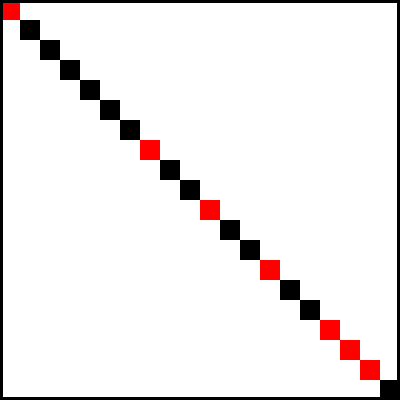
\includegraphics[width=4cm]{GRAPHICS/PGL_4_3/PGL_4_3_rep_3_0_draw} &
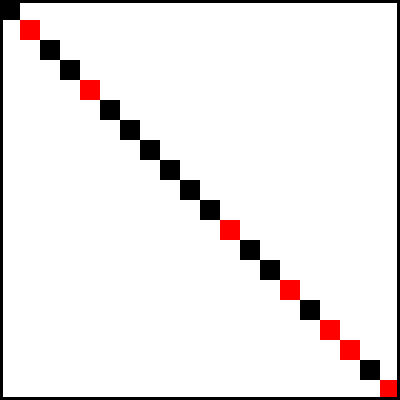
\includegraphics[width=4cm]{GRAPHICS/PGL_4_3/PGL_4_3_rep_3_1_draw} &
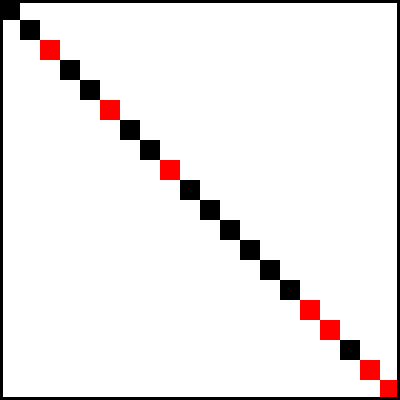
\includegraphics[width=4cm]{GRAPHICS/PGL_4_3/PGL_4_3_rep_3_2_draw} \\
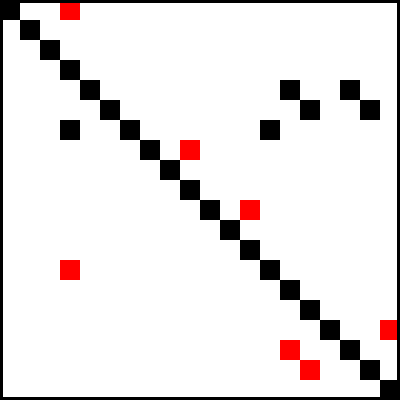
\includegraphics[width=4cm]{GRAPHICS/PGL_4_3/PGL_4_3_rep_3_3_draw} &
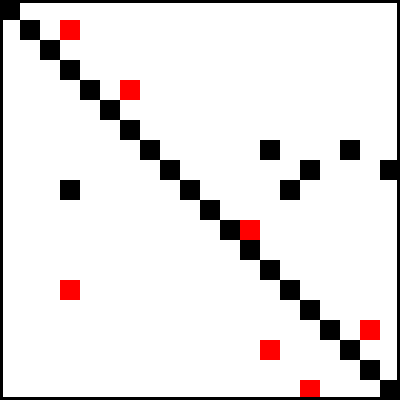
\includegraphics[width=4cm]{GRAPHICS/PGL_4_3/PGL_4_3_rep_3_4_draw} &
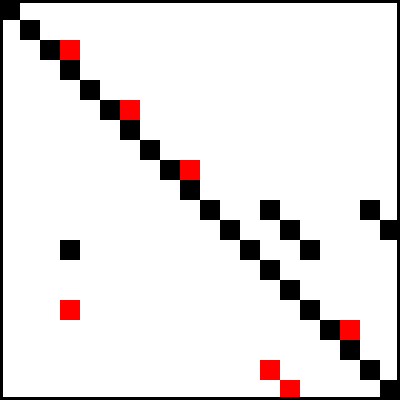
\includegraphics[width=4cm]{GRAPHICS/PGL_4_3/PGL_4_3_rep_3_5_draw} \\
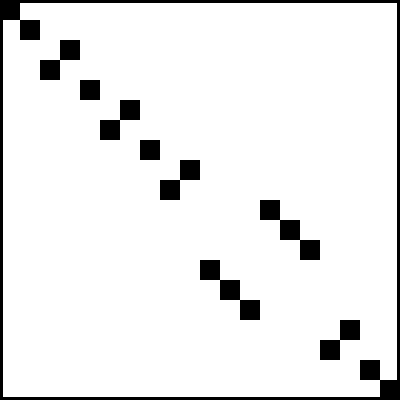
\includegraphics[width=4cm]{GRAPHICS/PGL_4_3/PGL_4_3_rep_3_6_draw} &
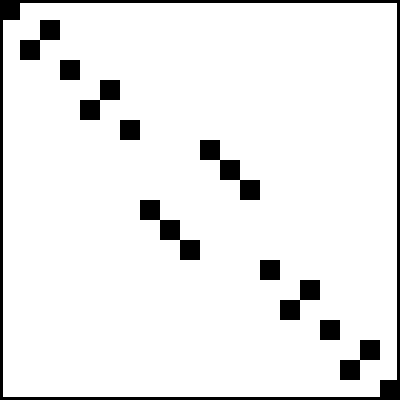
\includegraphics[width=4cm]{GRAPHICS/PGL_4_3/PGL_4_3_rep_3_7_draw} &
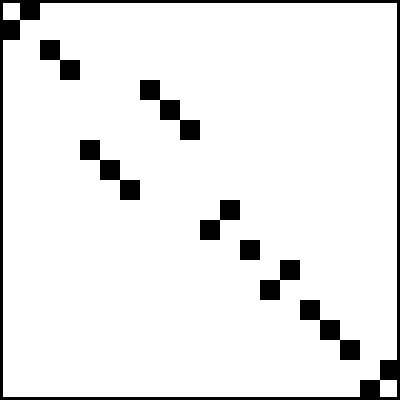
\includegraphics[width=4cm]{GRAPHICS/PGL_4_3/PGL_4_3_rep_3_8_draw} \\
\end{array}
$$
\caption{\label{fig:PGL43:rep}Representation of $\PGL(4,3)$ on cubic polynomials}
\end{figure}


In Table~\ref{tab:crypto}, some global cryptographic commands are shown.
\begin{table}
	\begin{center}
	\begin{tabular}{|p{4cm}|p{3cm}|p{7cm}|}
		\hline
		Command & Arguments & Purpose \\
		\hline
		\verb'-solovay_' \verb'strassen' & $a$ $n$  & Performs $n$ Solovay / Strassen tests on the number $a$\\
		\hline
		\verb'-miller_rabin' & $a$ $n$  & Performs $n$ Miller / Rabin tests on the number $a$\\
		\hline
		\verb'-fermat' & $a$ $n$  & Performs $n$ Fermat tests on the number $a$\\
		\hline
		\verb'-find_pseudoprime' & $a$ $n_1$ $n_2$ $n_3$  & Computes a pseudoprime which survives $n_1$ Fermat tests, $n_2$ Miller Rabin tests, $n_3$ Solovay Strassen tests\\
		\hline
		\verb'-find_strong_' \verb'pseudoprime' & $a$ $n_1$ $n_2$  & Computes a pseudoprime which survives $n_1$ Fermat tests and  $n_2$ Miller Rabin tests \\
		\hline
		\verb'-RSA_encrypt_text' & $d$ $n$ $b$ text & Using blocks of $b$ letters at a time, encrypt ``text'' using RSA with exponent $d$ modulo $n$\\
		\hline
		\verb'-RSA' & $d$ $n$  list-of-integers & encrypt the given sequence of integers using RSA with exponent $d$ modulo $n$\\
		\hline
\end{tabular}
\end{center}
\caption{\label{tab:crypto}Cryptographic Commands}
\end{table}
Some cryptographic commands require a finite field and appear as a finite field activity, see Table~\ref{tab:crypto2}.
\begin{table}
	\begin{center}
	\begin{tabular}{|p{4cm}|p{3cm}|p{7cm}|}
		\hline
		Command & Arguments & Purpose \\
		\hline
		\verb'-EC_add' & $a$ $b$ $i_1$ $i_2$ & On the elliptic curve $y^2\equiv x^3 + ax+b$ in $\bbF_q$, 
		add the points with indices $i_1$ and $i_2$, each given as a pair $x,y$\\
		\hline
		\verb'-EC_points' & $a$ $b$  & Computes all points of the elliptic curve $y^2\equiv x^3 + ax+b$ over $\bbF_q$ \\
		\hline
		\verb'-EC_multiple_of' & $a$ $b$ pt $n$ & Computes the $n$ fold multiple of the given point pt on the elliptic curve $y^2\equiv x^3 + ax+b$ over $\bbF_q$\\
		\hline
		\verb'-EC_cyclic_' \verb'subgroup' & $a$ $b$ pt  & Computes the cyclic subgroup generated by the given point pt on the elliptic curve $y^2\equiv x^3 + ax+b$ over $\bbF_q$\\
		\hline
		\verb'-EC_Koblitz_' \verb'encoding' & $a$ $b$ $s$ pt plain  & Computes the Koblitz encoding of ``plain'' (all caps) on the elliptic curve $y^2\equiv x^3 + ax+b$ over $\bbF_q$ using the base point pt and the secret exponent $s$ \\
		\hline
		\verb'-EC_bsgs' & $a$ $b$ pt $n$ cipher  & Prepare the baby-step giant-step tables for the ciphertext ``cipher'' on the elliptic curve $y^2\equiv x^3 + ax+b$ over $\bbF_q$ using the base point pt of order $n$\\
		\hline
		\verb'-EC_bsgs_decode' & $a$ $b$ pt $n$ cipher round-keys & Decodes the ciphertext ``cipher'' on the elliptic curve $y^2\equiv x^3 + ax+b$ over $\bbF_q$ using the base point pt of order $n$ and the round keys ``keys''\\
		\hline
		\verb'-EC_discrete_log' & $a$ $b$ pt base-pt & Computes the elliptic curve discrete log analogue of pt with respect to base-pt on the elliptic curve $y^2\equiv x^3 + ax+b$ over $\bbF_q$ \\
		\hline
		\verb'-NTRU_encrypt' & $N$ $p$ $H$ $R$ $M$ & NTRU encryption for the message $M(X)$ using the public key $H(X)$ and one-time-key $R(X)$. \\
		\hline
		\verb'-polynomial_' \verb'center_lift' & $A(X)$   & Compute the center lift mod $q$ for the coefficients of $A$ \\
		\hline
		\verb'-polynomial_' \verb'reduce_mod_p' & $p$ $A(X)$   &  Reduce the coefficients of the polynomial $A$ modulo $p$\\
		\hline
		\end{tabular}
	\end{center}
	\caption{\label{tab:crypto2}Finite Field Activities related to Cryptography}
	\end{table}
For instance,
{\tt
\input GRAPHICS/THE_MAKEFILE/EXTRACTS/EC_add.tex
}
adds the point $(1,4)$ on the curve $y^2 = x^3 + x + 3 \mod 11$ to itself.
The command 
{\tt
\input GRAPHICS/THE_MAKEFILE/EXTRACTS/EC_cyclic_subgroup.tex
}
computes the cyclic subgroup generated by the point $(1,4)$ on the curve $y^2 = x^3 + x + 3 \mod 11.$
The command
{\tt
\input GRAPHICS/THE_MAKEFILE/EXTRACTS/EC_points_199.tex
}
computes all points on the curve $y^2 = x^3 + 5x + 7 \mod 199$ 
and produces a bitmap drawing of the points in the affine plane 
shown in Figure~\ref{fig:EC:199:5:7:points}.
Both the $x$-axis and the $y$-axis are indexed by the field elements from 0 to 198.
\begin{figure}
$$
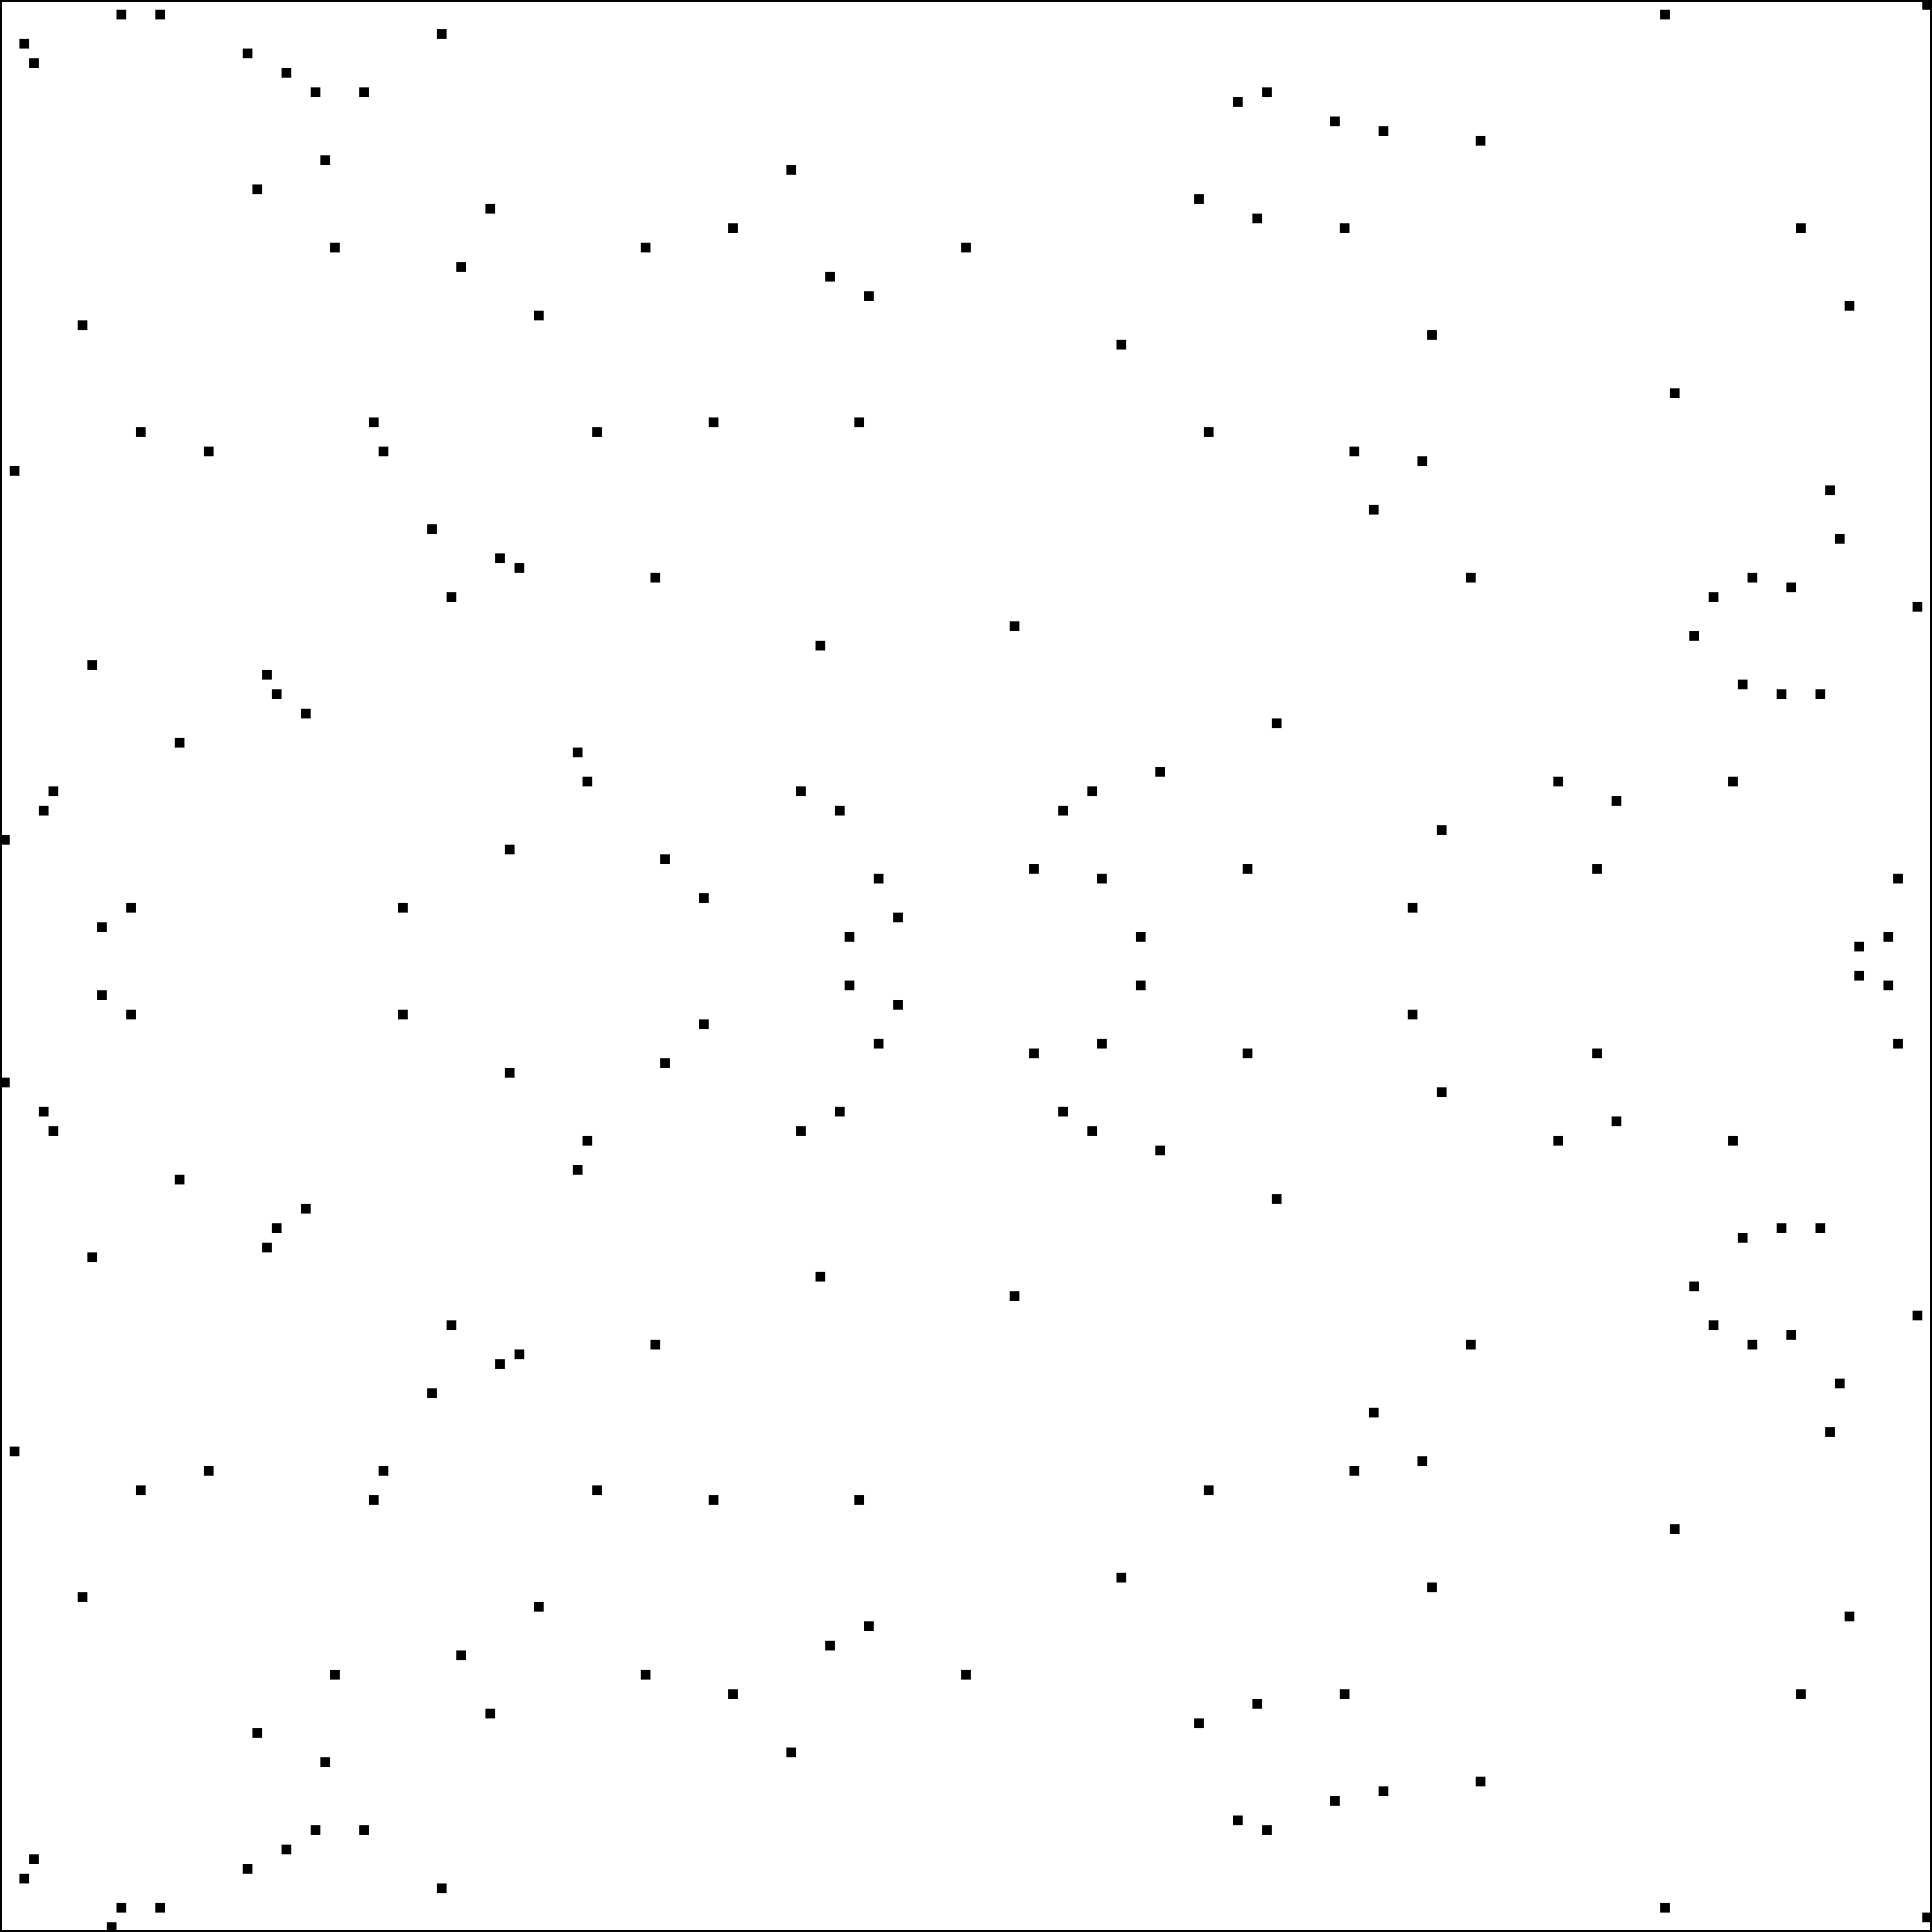
\includegraphics[width=11cm]{GRAPHICS/EC_199/EC_5_7_q199_points_xy_draw}
$$
\caption{\label{fig:EC:199:5:7:points}The elliptic curve $y^2 = x^3 + 5x + 7 \mod 199$}
\end{figure}


\bigskip

The command
{\tt
\input GRAPHICS/THE_MAKEFILE/EXTRACTS/EC_Koblitz_encoding.tex
}
encode the message ``DEADBEEF'' on the curve  $y^2 = x^3 + 5x + 7 \mod 199$ 
using the base point $(147,164)$ and the secret key $67.$
The $i$th input character is encoded as two points $(R_i,T_i)$ on the curve using the Elgamal scheme.
A random round key is generated for each plaintext symbol. 
As seen in this example, the \verb'-seed' command can be used to seed the random number generator with 
an arbitrary integer (here 17).

\bigskip


The command
{\tt
\input GRAPHICS/THE_MAKEFILE/EXTRACTS/EC_bsgs.tex
}
performs a baby-step-giant-step brute force attack on the ciphertext sequence
\begin{align*}
R_i &= (172,158),(45,195),(50,22),(10,103),(55,33),\\
&(50,22),(145,105),(31,74),(73,155),(67,60),(25,6),
\end{align*} 
using the base point $(147,164)$ on the curve  $y^2 = x^3 + 5x + 7 \mod 199,$ 
assuming a group order of $212.$ 
The command 
{\tt
\input GRAPHICS/THE_MAKEFILE/EXTRACTS/EC_bsgs_decode.tex
}
decodes the ciphertext sequence
\begin{align*}
T_i &= (127,188),(51,141),(85,29),(106,90),(41,105),(179,71),\\
&(171,2),(16,197),(183,72),(27,129),(37,10),
\end{align*} 
assuming round keys 
$$
k_i = 50,179,169,13,153,169,115,116,188,110,176,
$$
using the base point $(147,164)$ on the curve  $y^2 = x^3 + 5x + 7 \mod 199,$ 
and assuming a group order of $212.$ 

\bigskip


The next sequence of examples discusses the NTRU cryptosystem 
(cf. Example 7.53 in~\cite{Hoffstein2014}).
In the example, we choose the parameters of the cryptosystem to be $(N,p,q,d) = (7,41,3,2).$
Orbiter uses the following convention for polynomials over a finite field $\bbF_q$: 
The coefficients of $A(X) = a_0 + a_1X + \cdots + a_dX^d$ 
are listed as a sequence, starting with the constant term and ending with the leading coefficient.
The cryptosystem requires coefficients $a_i$ in the range $-\frac{p}{2} \le a_i \le \frac{p}{2}.$ 
So, in an extension to the conventionas for field elements in $\bbF_q$, 
Orbiter allows negative coefficients as well. 
The assumption is that $q$ is prime and 
negative coefficients are considered modulo $q.$
In the example, Alice picks the private polynomials 
$f(x) = x^6-x^4+x^3+x^2-1$ (with $d+1$ coefficients equal to 
plus one and $d$ coefficients equal to minus one) and 
$g(x) = x^6+x^4-x^2-x$ with $d$ coefficients plus one and $d$ coefficients minus one.
We also need the polynomial $x^N-1$. 
The makefile commands 
{\tt
\input GRAPHICS/THE_MAKEFILE/EXTRACTS/NTRU_N.tex
}
{\tt
\input GRAPHICS/THE_MAKEFILE/EXTRACTS/NTRU_P.tex
}
{\tt
\input GRAPHICS/THE_MAKEFILE/EXTRACTS/NTRU_Q.tex
}
{\tt
\input GRAPHICS/THE_MAKEFILE/EXTRACTS/NTRU_D.tex
}
{\tt
\input GRAPHICS/THE_MAKEFILE/EXTRACTS/NTRU_XN1.tex
}
{\tt
\input GRAPHICS/THE_MAKEFILE/EXTRACTS/ALICE_PRIVATE_F.tex
}
{\tt
\input GRAPHICS/THE_MAKEFILE/EXTRACTS/ALICE_PRIVATE_G.tex
}
are used to set up the appropriate variables according to these  choices. 

\bigskip


Regarding the NTRU set-up, Alice needs to compute her private keys 
$F_p(x)$ and $F_q(x).$ These two polynomials are defined as follows:
\begin{enumerate}
\item
	$F_p(x)$ is the inverse of $f(x)$ in $\bbF_p[x]/(x^n-1),$ 
\item
$F_q(x)$ the inverse of $f(x)$ in $\bbF_q[x]/(x^n-1).$
\end{enumerate}
To this end, we can use the \verb'extended_gcd_for_polynomials' 
command from Table~\ref{tab:nt}.
The following two makefile commands do the job: 
{\tt
\input GRAPHICS/THE_MAKEFILE/EXTRACTS/NTRU_Alice1.tex
}
{\tt
\input GRAPHICS/THE_MAKEFILE/EXTRACTS/ALICE_PRIVATE_FQ.tex
}
{\tt
\input GRAPHICS/THE_MAKEFILE/EXTRACTS/NTRU_Alice2.tex
}
The resulting polynomials 
(indicated as comments by means of the  \verb'#' symbol) 
are again encoded as makefile variables. 
{\tt
\input GRAPHICS/THE_MAKEFILE/EXTRACTS/ALICE_PRIVATE_FP
}
There is a chance that the polynommial 
$f(x)$ does not have an inverse in either $\bbF_p[x]$ 
or in $\bbF_q[x].$ 
In that case, Alice simply chooses a different 
polynomial $f(x)$ and tries again.
Alice can now compute her public key:
{\tt
\input GRAPHICS/THE_MAKEFILE/EXTRACTS/NTRU_Alice_public_key.tex
}
{\tt
\input GRAPHICS/THE_MAKEFILE/EXTRACTS/ALICE_PUBLIC_KEY.tex
}
The public key is assigned to the makefile variable \verb'ALICE_PUBLIC_KEY'.
Now, Bob chooses his message to Alice and his one-time-key. 
The message must be the center lift of a polynomial in $\bbF_p[x].$
The round-key must have exactly $d$ coefficients one 
and $d$ coefficients $-1$ (rest zeroes).
{\tt
\input GRAPHICS/THE_MAKEFILE/EXTRACTS/BOB_MESSAGE.tex
}
{\tt
\input GRAPHICS/THE_MAKEFILE/EXTRACTS/BOB_ONE_TIME_KEY.tex
}
The encryption proceeds using the \verb'NTRU_encrypt' command, 
and the result is stored in the makefile variable \verb'BOB_ENCRYPT':
{\tt
\input GRAPHICS/THE_MAKEFILE/EXTRACTS/NTRU_encrypt.tex
}
{\tt
\input GRAPHICS/THE_MAKEFILE/EXTRACTS/BOB_ENCRYPT.tex
}
Decryption is done in five steps. 
{\tt
\input GRAPHICS/THE_MAKEFILE/EXTRACTS/NTRU_decrypt1.tex
}
{\tt
\input GRAPHICS/THE_MAKEFILE/EXTRACTS/ALICE_C1.tex
}
{\tt
\input GRAPHICS/THE_MAKEFILE/EXTRACTS/NTRU_decrypt2.tex
}
{\tt
\input GRAPHICS/THE_MAKEFILE/EXTRACTS/ALICE_C2.tex
}
{\tt
\input GRAPHICS/THE_MAKEFILE/EXTRACTS/NTRU_decrypt3.tex
}
{\tt
\input GRAPHICS/THE_MAKEFILE/EXTRACTS/ALICE_C3.tex
}
{\tt
\input GRAPHICS/THE_MAKEFILE/EXTRACTS/NTRU_decrypt4.tex
}
{\tt
\input GRAPHICS/THE_MAKEFILE/EXTRACTS/ALICE_C4.tex
}
{\tt
\input GRAPHICS/THE_MAKEFILE/EXTRACTS/NTRU_decrypt5.tex
}
Decryption produces Bob's message to Alice.

\bigskip

ToDo:

\begin{itemize}
\item
RSA
\item
sqrt mod
\item
quadratic sieve
\item
pseudoprimes
\end{itemize}

\bigskip

\label{sec:coding}



\section{Introduction}
\input C10/sec_1.tex


\clearpage

\section{Linear Codes}
\label{sec:linear:codes}



\input C10/sec_2.tex


\clearpage

\section{Golay Codes}
\label{sec:Golay}



\input C10/sec_3.tex


\clearpage

\section{CRC Codes}
\label{sec:CRC}



\input C10/sec_4.tex


\clearpage

\section{Reed-Muller Codes}
\label{sec:Reed:Muller}



\input C10/sec_5.tex


\clearpage

\section{BCH Codes}
\label{sec:BCH}



\input C10/sec_6.tex


\clearpage

\section{Reed-Solomon Codes}
\label{sec:Reed:Solomon}



\input C10/sec_7.tex


\clearpage

\section{Bounds}
\label{sec:Bounds}



\input C10/sec_8.tex


\clearpage

\section{Classification of Optimal Linear Codes}
\label{sec:coding:classification}



\input C10/sec_9.tex


\clearpage
Orbiter supports research in coding thory. 
Global Orbiter commands for coding theory 
are summarized in Table~\ref{tab:coding:global}. 
Additional commands, associated with objects of type code will be discussed below and in later sections.
\begin{table}
	\begin{center}
	\begin{tabular}{|p{4cm}|p{3cm}|p{7cm}|}
		\hline
		Command & Arguments & Purpose \\
		\hline
		\hline
		\verb'-make_macwilliams' \verb'_system' & $q$ $n$ $k$ & Create the MacWilliams equations for the weight enumerator of the dual code. \\
		\hline
		\verb'-table_' \verb'of_bounds' & $n_{\max}$ $q$ & Make a table of bounds for $q$-ary linear code for all $k \le n \le n_{\max}$ \\
		\hline
		\verb'-make_bounds_' \verb'for_d_given_n_' \verb'and_k_and_q' & $n$ $k$ $q$ & Make bounds for the minimum distance of a $[n,k]_q$ code\\
		\hline
		\verb'-Hamming_space_' \verb'distance_matrix' & $n$ $q$ & Make the distance matrix of the Hamming graph $H(n,q).$ \\
		\hline
		\verb'-random_noise_' \verb'in_bitmap_file' & $f1$ $f2$ $n$ $d$ & Apply random noise a the $d/n$ level to the bitmap file $f1$ and write to $f2.$ \\
		\hline
		\verb'-introduce_errors' & CRC-options & 
		Introduce errors to a file. See Table~\ref{tab:CRC:options}.\\
		\hline
		\verb'-check_errors' & CRC-options & 
		Find errors in a CRC coded file. See Table~\ref{tab:CRC:options}.\\
		\hline
		\verb'-extract_block' & CRC-options & 
		Extract a block from a CRC coded file. See Table~\ref{tab:CRC:options}. \\
		\hline
		\end{tabular}
	\end{center}
	\caption{\label{tab:coding:global}Global Coding Theoretic Commands}
	\end{table}

\bigskip



The command 
{\tt
\input GRAPHICS/THE_MAKEFILE/EXTRACTS/Allen_Gates_noise_1_percent.tex
}
simulates random noise at the 1 percent level applied to the file \verb'allen_Gates.bmp', see Figure~\ref{fig:allen:gates:1percent}. 
\begin{figure}
$$
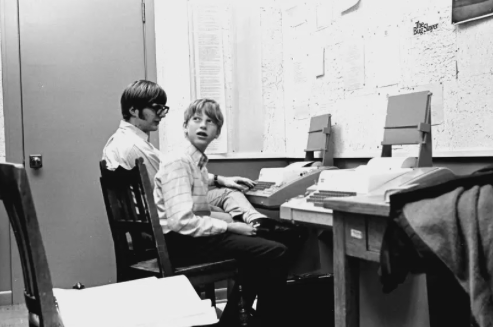
\includegraphics[width=8cm]{GRAPHICS/CODING_THEORY/allen_Gates}
\quad
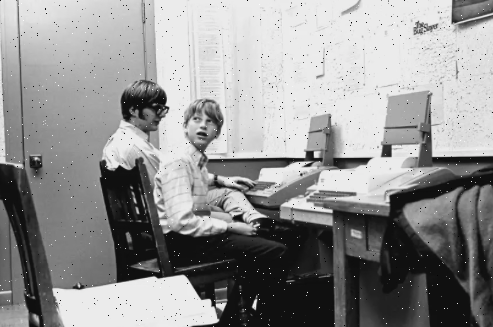
\includegraphics[width=8cm]{GRAPHICS/CODING_THEORY/allen_Gates_1}
$$
\caption{\label{fig:allen:gates:1percent}Random noise at the 1\% level}
\end{figure}
The original is on the left. 
The effect of noise can be seen on the right.
The picture 
shows Paul Allen and Bill Gates in the early 1970s. 

\bigskip

The command
{\tt
\input GRAPHICS/THE_MAKEFILE/EXTRACTS/Hamming_space_4_2_distance_matrix.tex
}
creates the distance matrix of the Hamming graph $H(n,q).$ 
The data is written to the file \verb'Hamming_n4_q2.csv'. 
The command
{\tt
\input GRAPHICS/THE_MAKEFILE/EXTRACTS/Hamming_space_4_2_distance_matrix_draw.tex
}
produces the bitmap graphic \verb'Hamming_n4_q2_draw.bmp'
shown in Figure~\ref{fig:Hamming42}.
\begin{figure}
$$
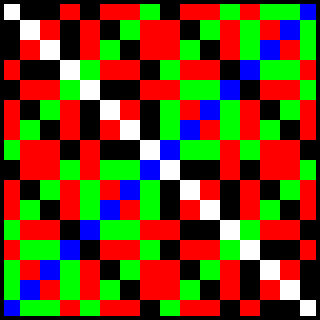
\includegraphics[width=8cm]{GRAPHICS/CODES/Hamming_n4_q2_draw}
$$
\caption{\label{fig:Hamming42}The color-coded distance matrix of the Hamming graph $H(4,2)$}
\end{figure}




\bigskip


The command
{\tt
\input GRAPHICS/THE_MAKEFILE/EXTRACTS/Hamming_code_macwilliams.tex
}
creates the coefficient matrix of the MacWilliams system for the $[7,4,2]$ Hamming code:
\begin{mdframed}[style=MyFrame]
\input GRAPHICS/LATEX/code_MacWilliams_Hamming.tex
\end{mdframed}



\bigskip

For examples concerning the bounds, see Section~\ref{sec:Bounds}.

\bigskip




Tables~\ref{tab:finitefield:activities:coding1} and~\ref{tab:finitefield:activities:coding2} list coding theoretic activities in Orbiter. 
Depending on the activity, an object of type code or an object of type finite field is required.
\begin{table}
	\begin{center}
	\begin{tabular}{|p{4cm}|p{3cm}|p{7cm}|}
		\hline
		Command & Arguments & Purpose \\
		\hline
		\hline
		\verb'-BCH' & $n$ $q$ $t$  & Compute a table of BCH codes of length $n$ over $\bbF_q$. \\
		\hline
		\verb'-BCH_dual' &   &  \\
		\hline
		\verb'-general_code_' \verb'binary' &  $n$ text &  \\
		\hline
		\verb'-code_diagram' & label codewords n  &  \\
		\hline
		\verb'-code_diagram_' \verb'from_file' & fname  &  \\
		\hline
		\verb'-enhance' &  radius &  \\
		\hline
		\verb'-metric_balls' & radius  &  \\
		\hline
		\verb'-long_code' & $n$ generators  &  \\
		\hline
		\verb'-encode_text_5bits' & input fname  &  \\
		\hline
		\verb'-field_induction' & fname-in fname-out nb-bits  &  \\
		\hline
		\verb'-crc32' & text  &  \\
		\hline
		\verb'-crc32_hexdata' & hexdata  &  \\
		\hline
		\verb'-crc32_test' &  block-length &  \\
		\hline
		\verb'-crc256_test' & message-length $R$ $k$  &  \\
		\hline
		\verb'-crc32_remainders' & msg-length  &  \\
		\hline
		\verb'-crc32_file_based' & fname-in fname-out block-length  &  \\
		\hline
		\verb'-crc_new_file_based' & fname  &  \\
		\hline
		\verb'-weight_enumerator' &  matrix &  
		Compute the complete weight enumerator of the 
		linear code generated by the $m \times n$ matrix $L$  \\
		\hline
		\end{tabular}
	\end{center}
	\caption{\label{tab:finitefield:activities:coding1}Coding Theoretic Activities (Part I)}
	\end{table}
\begin{table}
	\begin{center}
	\begin{tabular}{|p{4cm}|p{3cm}|p{7cm}|}
		\hline
		Command & Arguments & Purpose \\
		\hline
		\hline
		\verb'-minimum_distance' &  code-object-label &  
		Compute the minimum distance of the linear code object.  \\
		\hline
		\verb'-generator_matrix_' \verb'cyclic_code' & $n$ poly  &  \\
		\hline
		\verb'-nth_roots' & $n$  &  \\
		\hline
		\verb'-make_BCH_code_' \verb'and_encode' & $n$ $d$ text fname  &  \\
		\hline
		\verb'-NTT' & $n$ $q$  &  \\
		\hline
		\verb'-find_CRC_' \verb'polynomials' & nb-errors info-bits check-bits  &  \\
		\hline
		\verb'-write_code_' \verb'for_division' &  fname $A$ $B$ &  \\
		\hline
		\verb'-polynomial_' \verb'division_from_file' &  fname $r1$ &  \\
		\hline
		\verb'-polynomial_' \verb'division_from_' \verb'file_all_k_bit_' \verb'error_patterns' &  fname $r1$ $k$ &  \\
		\hline
		\verb'-export_magma' &  fname &  \\
		\hline
		\verb'-export_codewords' & fname  &  \\
		\hline
		\verb'-export_genma' &  fname &  \\
		\hline
		\verb'-export_checkma' & fname  &  \\
		\hline
		\end{tabular}
	\end{center}
	\caption{\label{tab:finitefield:activities:coding2}Coding Theoretic Activities (Part II)}
	\end{table}


\bigskip


The following command creates the $[5,2]_2$ code whose codewords are $\{0,7,25,30\}$:
{\tt
\input GRAPHICS/THE_MAKEFILE/EXTRACTS/CODE_5_2_3_CODEWORDS.tex
}
{\tt
\input GRAPHICS/THE_MAKEFILE/EXTRACTS/code_5_2_3_diagram.tex
}
The Hamming graph $H(5,2)$ can be created with the following command:
{\tt
\input GRAPHICS/THE_MAKEFILE/EXTRACTS/Hamming_5_2_graph.tex
}
Using the unix dot program, this command sequence creates the drawing of $H(5,2)$ 
shown in Figure~\ref{fig:H52:drawing}.
\begin{figure}
$$
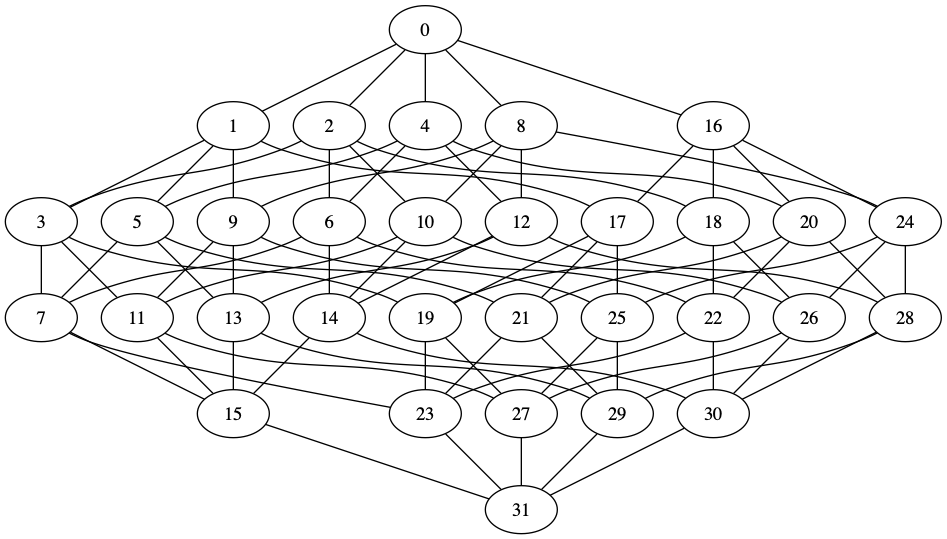
\includegraphics[width=15cm]{GRAPHICS/CODES/Hamming_5_2}
$$
\caption{\label{fig:H52:drawing}Drawing of the Hamming graph $H(5,2)$}
\end{figure}

\bigskip



In this section, we will see how linear codes can be created and studied in Orbiter. 
A code object is used to represent a specific code. 
Table~\ref{tab:code:object} list the commands  to create a code object. 
\begin{table}
	\begin{center}
	\begin{tabular}{|p{4cm}|p{3cm}|p{7cm}|}
		\hline
		Command & Arguments & Purpose \\
		\hline
		\hline
		\verb'-field' & $F$ & Specify the field of definition. \\
		\hline
		\verb'-linear_code_' \verb'through_generator_' \verb'matrix' & $M$ & Create a code defined by a generator matrix. \\
		\hline
		\verb'-linear_code_from_' \verb'projective_set' & $nmk$ $S$ & Create a code defined by a projective set in the dual. \\
		\hline
		\verb'-linear_code_by_' \verb'columns_of_parity_' \verb'check' & $nmk$ $M$ & Create a code defined by a affine set in the dual. \\
		\hline
		\verb'-first_order_' \verb'Reed_Muller' & $m$ & Create a first order Reed-Muller code of degree $m$. \\
		\hline
		\verb'-BCH' & $n$ $d$ & BCH code of length $n$ with prescribed minimum distance $d$. \\
		\hline
		\verb'-Reed_Solomon' & $n$ $d$ &  Not yet implemented. \\
		\hline
		\verb'-Gilbert_Varshamov' & $n$ $k$ $d$ & Create a Gilbert-Varshamov code of length $n$ with dimension $k$ and minimum distance at least $d.$ \\
		\hline
		\end{tabular}
	\end{center}
	\caption{\label{tab:code:object}Commands to Create Codes}
	\end{table}
Table~\ref{tab:code:object:modifications} list code modifications. 
These are commands used to create a new code from an old one. 
\begin{table}
	\begin{center}
	\begin{tabular}{|p{4cm}|p{3cm}|p{7cm}|}
		\hline
		Command & Arguments & Purpose \\
		\hline
		\hline
		\verb'-dual' &  & Compute the dual code. \\
		\hline
		\end{tabular}
	\end{center}
	\caption{\label{tab:code:object:modifications}Code modifications}
	\end{table}

\bigskip


The following command creates the first order Reed-Muller code in three variables:
{\tt
\input GRAPHICS/THE_MAKEFILE/EXTRACTS/RM_3_1.tex
}
Let us create the Hamming code.
The dual of the Hamming code is the simplex code, so we create the simplex code first.
The following makefile variable is defined to hold the generator matrix of the simplex code:
{\tt
\input GRAPHICS/THE_MAKEFILE/EXTRACTS/SIMPLEX_CODE_GENERATOR.tex
}
The following command computes the nullspace of this matrix, which is the Hamming code:
{\tt
\input GRAPHICS/THE_MAKEFILE/EXTRACTS/simplex_code.tex
}
The following latex output is produced:
\begin{mdframed}[style=MyFrame]
\input GRAPHICS/LATEX/code_simplex.tex
\end{mdframed}

\bigskip

It is possible to create the Hamming code by taking the dual of the simplex code. 
The following command does so:
{\tt
\input GRAPHICS/THE_MAKEFILE/EXTRACTS/Hamming_code.tex
}
The command also exports the code to magma by means of the magma file \verb'Hamming.magma', shown below:
\begin{verbatim}
K<w> := GF(2);
V := VectorSpace(K, 7);
C := LinearCode(sub<V |
[1,1,1,0,0,0,0],
[1,0,0,1,1,0,0],
[0,1,0,1,0,1,0],
[1,1,0,1,0,0,1]>);
\end{verbatim}


\bigskip

The next command creates the first order Reed-Muller code in $3$ variables. 
All codewords are created.
The codewords and the generator matrix are exported to files.
{\tt
\input GRAPHICS/THE_MAKEFILE/EXTRACTS/RM_3_1_and_codewords.tex
}
Alternatively, we can store the generator matrix in a makefile variable: 
{\tt
\input GRAPHICS/THE_MAKEFILE/EXTRACTS/CODE_RM_3_1_GENMA.tex
}
The following command creates the Hamming code from its 
generator matrix directly:
{\tt
\input GRAPHICS/THE_MAKEFILE/EXTRACTS/RM_3_1_from_generator_matrix.tex
}

\bigskip


%Suppose we want to look at the codewords of the Hamming code in the Hamming space. 
%The following command will produce Figure~\ref{fig:Hamming}.
The following command creates the Hamming code and produces a list of codewords.
{\tt
\input GRAPHICS/THE_MAKEFILE/EXTRACTS/RM_3_1_and_codewords.tex
}
\begin{figure}
$$

\includegraphics[width=4cm]{GRAPHICS/code_matrix_16_8_draw}
$$
\caption{\label{fig:Hamming}The Hamming code}
\end{figure}

\bigskip



The Hamming code is cyclic. 
To see this, we need to consider the action of the Singer cycle on
the set of points of $\PG(2,2).$
The following command creates the Singer cycle:
{\tt
\input GRAPHICS/THE_MAKEFILE/EXTRACTS/Hamming_singer.tex
}
This produces the following output:
\begin{mdframed}[style=MyFrame]
\input GRAPHICS/LATEX/code_Hamming_singer.tex
\end{mdframed}
From this, we know how to rearrange the points 
of $\PG(2,2)$ to exhibit the cyclic structure.
We issue the following command to recreate the Hamming code:
{\tt
\input GRAPHICS/THE_MAKEFILE/EXTRACTS/SIMPLEX_CODE_GENMA_CYCLIC.tex
}
{\tt
\input GRAPHICS/THE_MAKEFILE/EXTRACTS/Hamming_cyclic_generator.tex
}
This produces the following output:
\begin{mdframed}[style=MyFrame]
\input GRAPHICS/LATEX/code_Hamming_cyclic.tex
\end{mdframed}

\bigskip

Orbiter can compute the weight enumerator and the minimum distance of codes.
Let us consider the Hamming code, for example.
We use a makefile variable for the generator matrix: 
{\tt
\input GRAPHICS/THE_MAKEFILE/EXTRACTS/HAMMING_CODE_GENERATOR.tex
}
The next command computes the weight enumerator:
{\tt
\input GRAPHICS/THE_MAKEFILE/EXTRACTS/Hamming_weight_enumerator.tex
}
We find that the weight enumerator is
$$
( 1, 0, 0, 7, 7, 0, 0, 1 ).
$$
The next command computes the minimum distance of the code:
{\tt
\input GRAPHICS/THE_MAKEFILE/EXTRACTS/Hamming_minimum_distance.tex
}
The following command computes the minimum distance 
of the Golay code of length $23$:
{\tt
\input GRAPHICS/THE_MAKEFILE/EXTRACTS/Golay23_minimum_distance.tex
}


The Golay code of length 23 is a perfect code of dimension 12 and minimum distance 7.
The metric balls of radius three centered around codewords cover the whole Hamming space.
We can create the code by listing the columns of a generator matrix in Orbiter ranks of points in $\PG(11,2)$.
The following makefile variable does that:
{\tt
\input GRAPHICS/THE_MAKEFILE/EXTRACTS/GOLAY_23_COLUMN_RANKS_PROJECTIVELY.tex
}
Suppose we want to list the code words. The following command can be used:
{\tt
\input GRAPHICS/THE_MAKEFILE/EXTRACTS/Golay23_code_words.tex
}

A CRC code can be used to detect communication errors. 
It is a cyclic code, and hence generated by a polynomial over a finite field. 
The message is encoded as a string, which is then thought of as a polynomial, 
called the information polynomial. 
Assume that the check polynomial has degree $d$.
The information polynomial is then divided by the check polynomial. 
The remainder is added to the information polynomial multiplied by $X^d.$
This is the codeword, which is sent.

\bigskip

Table~\ref{tab:CRC:options} summarizes options associated with commands for CRC-codes. 
\begin{table}
	\begin{center}
	\begin{tabular}{|p{4cm}|p{3cm}|p{7cm}|}
		\hline
		Command & Arguments & Purpose \\
		\hline
		\hline
		\verb'-input' & fname & Input file name. \\
		\hline
		\verb'-output' & fname & Output file name. \\
		\hline
		\verb'-block_length' & $L$ & Set block length to $L$ field elements. \\
		\hline
		\verb'-block_based_' \verb'error_generator' &  & Apply block-based error generator. \\
		\hline
		\verb'-file_based_' \verb'error_generator' & threshold & Apply file-based error generator. \\
		\hline
		\verb'-nb_repeats' & $N$ & Set the number of repeats to $N$. \\
		\hline
		\verb'-threshold' & $t$ & Set probability of error per experiment to $t/1000000$. \\
		\hline
		\verb'-error_log' & fname & Set file name for error logging. \\
		\hline
		\verb'-selected_block' & $i$ & Set block number. \\
		\hline
		\end{tabular}
	\end{center}
	\caption{\label{tab:CRC:options}CRC options}
	\end{table}


\bigskip

Here is an example. 
We consider a short string of English text and encode it with 5 bits per character. 
This is done using the \verb'-encode_text_5bits' command. 
The encoded text is stored in a csv file, which we decide to call \verb'text.csv'.
{\tt
\input GRAPHICS/THE_MAKEFILE/EXTRACTS/encode_text_5bits.tex
}
We decide to pick the binary polynomial $13 = X^3+X^2+1$.
We divide the information polynomial by the check polynomial: 
{\tt
\input GRAPHICS/THE_MAKEFILE/EXTRACTS/encode_text_5bits_check.tex
}
This creates the following output:
\begin{mdframed}[style=MyFrame]
{\small
\input GRAPHICS/LATEX/CRC_polynomial_division.tex
}
\end{mdframed}
The remainder after division by the check polynomial is 5, or 
the polynomial $X^2+1,$ or the bit-sequence $101.$ 


\bigskip


The following command investigates all 1-bit errors, to see which of them can be detected
using the given CRC-polynomial: 
{\tt
\input GRAPHICS/THE_MAKEFILE/EXTRACTS/encode_text_5bits_1error.tex
}
The following output is created:
\begin{mdframed}[style=MyFrame]
{\small
\input GRAPHICS/LATEX/CRC_table_of_remainders.tex
}
\end{mdframed}
It shows that 5 single bit errors are undetected.

\bigskip

The following command performs an exhaustive search over all binary CRC polynomials of degree $k=10$ 
which can detect every error pattern of Hamming weight at most $t=3$ in messages of length $n=128.$ 
{\tt
\input GRAPHICS/THE_MAKEFILE/EXTRACTS/CRC_3_128_10.tex
}
The program finds 244 polynomials in about 1 minute.



\bigskip

Here is a collection of CRC polynomials from various sources:
{\tt
\input GRAPHICS/THE_MAKEFILE/EXTRACTS/CRC4.tex
}
{\tt
\input GRAPHICS/THE_MAKEFILE/EXTRACTS/CRC7.tex
}
{\tt
\input GRAPHICS/THE_MAKEFILE/EXTRACTS/CRC8_ATM.tex
}
{\tt
\input GRAPHICS/THE_MAKEFILE/EXTRACTS/CRC16_CCITT.tex
}
{\tt
\input GRAPHICS/THE_MAKEFILE/EXTRACTS/CRC32_ETHERNET.tex
}
{\tt
\input GRAPHICS/THE_MAKEFILE/EXTRACTS/CRC32_CASTAGNOLI.tex
}
{\tt
\input GRAPHICS/THE_MAKEFILE/EXTRACTS/CRC64_ECMA182.tex
}
{\tt
\input GRAPHICS/THE_MAKEFILE/EXTRACTS/CRC64_ROCKSOFT.tex
}


\bigskip


%We test an incorrect implementation of CRC32:
%{\tt
%\input GRAPHICS/THE_MAKEFILE/EXTRACTS/crc32_test.tex
%}
%{\tt
%\input GRAPHICS/THE_MAKEFILE/EXTRACTS/crc32_test_hexdata.tex
%}

We test whether the polynomial crc32 is irreducible:
{\tt
\input GRAPHICS/THE_MAKEFILE/EXTRACTS/crc32_Berlekamp_matrix.tex
}

\bigskip

Now, we create some new CRC polynomials over the field $\bbF_{256}.$
To begin with, we create the 771st roots over $\bbF_{256}$:
{\tt
\input GRAPHICS/THE_MAKEFILE/EXTRACTS/CRC_F256_roots_771.tex
}
We create a BCH code of length 771 over $\bbF_{256}$ with designed distance 2:
{\tt
\input GRAPHICS/THE_MAKEFILE/EXTRACTS/CRC_F256_BCH_code_d2.tex
}
The polynomial in dense coding
{\tt
\input GRAPHICS/THE_MAKEFILE/EXTRACTS/CRC_POLY_Q256_DEG2_DENSE.tex
}
We generate C++ source code for the use of this polynomial:
{\tt
\input GRAPHICS/THE_MAKEFILE/EXTRACTS/CRC_F256_BCH_write_code_for_division_d2.tex
}
We create a BCH code of length 771 over $\bbF_{256}$ with designed distance 16:
{\tt
\input GRAPHICS/THE_MAKEFILE/EXTRACTS/F256_BCH_code_d16.tex
}
The polynomial in sparse coding is:
{\tt
\input GRAPHICS/THE_MAKEFILE/EXTRACTS/POLY_Q256_DEG30_SPARSE.tex
}
The polynomial in dense coding is:
{\tt
\input GRAPHICS/THE_MAKEFILE/EXTRACTS/POLY_Q256_DEG30_DENSE.tex
}
We generate C++ source code for the use of this polynomial:
{\tt
\input GRAPHICS/THE_MAKEFILE/EXTRACTS/F256_BCH_write_code_for_division_d16.tex
}


%The generator polynomial is printed in two ways, sparse and dense. 
%The notion of sparse and dense agrees with that of Section~\ref{sec:vector:builder}.
%Dense means that the coefficient vector of the polynomial is listed in full.
%Sparse means that only the nonzero terms are listed as pairs, the nonzero coefficient and the index of %the term. 
%The coefficient vector determines the generator polynomial 
%$g(X) \in \bbF_{256}[X]$ of the BCH code of length $771$ over $\bbF_{256}.$
%Next, we test if $g(x)$ divides $X^{771}-1$, as it should:
%{\tt
%\input GRAPHICS/THE_MAKEFILE/EXTRACTS/POLY_Q256_DEG30_DENSE.tex
%}
We confirm that the polynomial divides $X^{771}-1$ as it should:
{\tt
\input GRAPHICS/THE_MAKEFILE/EXTRACTS/F256_BCH_code_d16_division.tex
}
%This confirms that the remainder after dividing $X^{771}-1$ by $g(X)$ is indeed zero.
The next example introduces three errors. 
The remainder is not zero, so the errors are detected:
{\tt
\input GRAPHICS/THE_MAKEFILE/EXTRACTS/F256_BCH_code_d16_error.tex
}








The following command creates the Reed Muller code $\mbox{RM}_{3,1}.$ 
{\tt
\input GRAPHICS/THE_MAKEFILE/EXTRACTS/RM_3_1_Hamming_space_diagram.tex
}
The following command produces a diagram of the characteristic 
function of the code in the Hamming space $H(8,2),$
shown in Figure~\ref{fig:RM31codewords:Hamming}. 
The different codewords are given different colors.
{\tt
\input GRAPHICS/THE_MAKEFILE/EXTRACTS/RM_3_1_draw.tex
}
\begin{figure}
$$

\includegraphics[width=5cm]{GRAPHICS/RM/RM_3_1_diagram_8_16_draw}
$$
\caption{\label{fig:RM31codewords:Hamming}Boolean function representation of ${\rm RM}_{3,1}$ in $H(8,2)$}
\end{figure}



Let $\beta$ be an $n$-th root of unity over $\bbF_q$. 
The minimum polynomial of $\beta$ over $\bbF_q$ is denoted as $m_{\beta,\bbF_q}.$
The BCH code of length $n$ and designed distance $d$ is 
the cyclic code with generator polynomial 
$$
{\rm lcm}\Big(m_{\beta^1,\bbF_q}, m_{\beta^2,\bbF_q},\ldots, m_{\beta^{d-1},\bbF_q}\Big).
$$
To create the polynomial $m_{\beta^a,\bbF_q}$, we consider the $q$-cyclotomic set of $a$ modulo $n,$ 
which is 
$$
\{aq^i \mod n \mid i \in \bbZ \}.
$$

\bigskip

Suppose we want to make a BCH-code of length $21$ over $\bbF_8.$
In Section~\ref{sec:extension:fields}, we considered the $q$-cyclotomic sets modulo $21$ for $q=8.$
Let us produce a pictorial representation. Omitting the singletons, a transversal is given by the 
sets containing $1,2,4,5,7,10,13.$ For this reason, we issue the command 
{\tt
\input GRAPHICS/THE_MAKEFILE/EXTRACTS/draw_cyclotomic_mod_21_q8.tex
}
The output is shown in Figure~\ref{fig:cyc:21:q8}.
\begin{figure}
$$
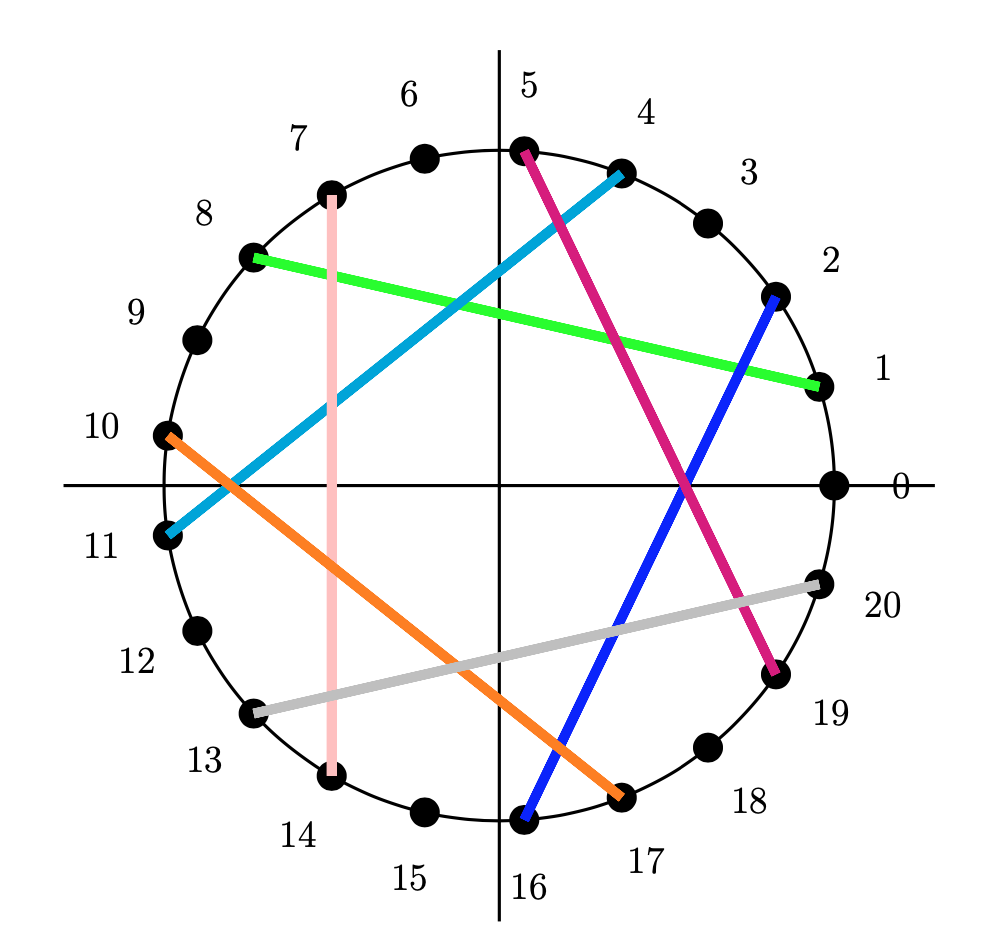
\includegraphics[width=9cm]{GRAPHICS/BCH/mod_21_q8}
$$
\caption{\label{fig:cyc:21:q8}The $8$-cyclotomic sets modulo $21$}
\end{figure}
We will try BCH-codes with minimum distances $3,$ $5$ and $7$.
Here is distance $3$:
{\tt
\input GRAPHICS/THE_MAKEFILE/EXTRACTS/F_8_BCH_code_d3.tex
}
The code is described in a latex output file:
\begin{mdframed}[style=MyFrame]
\input GRAPHICS/LATEX/code_BCH_8_3.tex
\end{mdframed}

\bigskip

And now for $d=5$:
{\tt
\input GRAPHICS/THE_MAKEFILE/EXTRACTS/F_8_BCH_code_d5.tex
}
The output file is:
\begin{mdframed}[style=MyFrame]
\input GRAPHICS/LATEX/code_BCH_8_5.tex
\end{mdframed}


We compute the minimum distance:
{\tt
\input GRAPHICS/THE_MAKEFILE/EXTRACTS/F_8_BCH_code_d5_minimum_distance.tex
}
The minimum distance turns out to be $d=5$.


\bigskip

Finally, we create the BCH code with minimum distance $d=7$:
{\tt
\input GRAPHICS/THE_MAKEFILE/EXTRACTS/F_8_BCH_code_d7.tex
}
The output file is:
\begin{mdframed}[style=MyFrame]
\input GRAPHICS/LATEX/code_BCH_8_7.tex
\end{mdframed}



\bigskip



As a larger example, let us consider the 2-cyclotomic sets of $2$ and $3$ modulo 255. 
The following command produces 
a graphical representation on a circle (similar to the unit circle in complex analysis). 
The $255$-th roots of unity are placed in the appropriate position.
{\tt
\input GRAPHICS/THE_MAKEFILE/EXTRACTS/draw_mod_255_cyclotomic_1_and_3.tex
}
The drawing is shown in Figure~\ref{fig:BCH:cyclotomic}.
\begin{figure}
$$
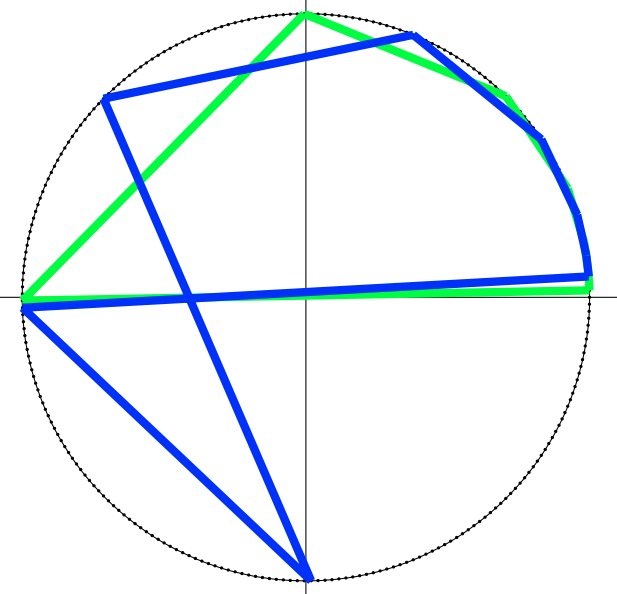
\includegraphics[width=8cm]{GRAPHICS/CODES/BCH_255_cyclotomic_stets_1_3}
$$
\caption{\label{fig:BCH:cyclotomic}Cyclotomic sets modulo 255}
\end{figure}

\bigskip

Suppose we want to make a BCH-code over $\bbF_{256}.$
In order to keep the degree of the generator polynomial low, we try a quadratic field extension. 
This way, each cyclotomic set has size either 1 or 2.
Since 
$$
256^2-1 = (256+1)(256-1) = 257 \cdot 3 \cdot 5 \cdot 17,
$$
we can consider a code of length $n=771=257\cdot 3.$ 
The following command computes the $256$-cyclotomic cosets modulo 771:
{\tt
\input GRAPHICS/THE_MAKEFILE/EXTRACTS/BCH_F256_roots_771.tex
}
The next command creates a BCH-code of length 771 over $\bbF_{256}$ with minimum distance at least 16:
{\tt
\input GRAPHICS/THE_MAKEFILE/EXTRACTS/BCH_F256_BCH_code_d16.tex
}

\bigskip

Reed-Solomon codes are BCH-codes where the length $n$ divides $q-1.$
In particular, they are cyclic codes. They are almost never binary.

\bigskip

To create a Reed-Solomon code over $\bbF_7$, we use the primitive element $\alpha=3$.
The Reed-Solomon code of designed distance 3 over $\bbF_7$ is the cyclic code generated by 
$$
(X-\alpha)(X-\alpha^2) = (X-3)(X-2)= X^2+2X+6.
$$
The generator matrix of the code in cyclic form is
$$
\left[
\begin{array}{*{6}c}
6  & 2  & 1  & 0  & 0  & 0\\
0  & 6  & 2  & 1  & 0  & 0\\
0  & 0  & 6  & 2  & 1  & 0\\
0  & 0  & 0  & 6  & 2  & 1\\
\end{array}
\right].
$$
Let us investigate this code. We start with the weight enumerator. 
The command 
{\tt
\input GRAPHICS/THE_MAKEFILE/EXTRACTS/CODE_RS_6_4_7.tex
}
{\tt
\input GRAPHICS/THE_MAKEFILE/EXTRACTS/RREF_RS_6_4_7_weight_enumerator.tex
}
computes the weight enumerator, which turns out to be
$$
( 1, 0, 0, 120, 360, 972, 948 ).
$$
In polynomial form, this is
$$
1y^6 + 120x^3y^3 + 360x^4y^2 + 972x^5y + 948x^6.
$$
This confirms that the minimum distance is three.

\bigskip

Let us consider an example of a Reed-Solomon code in characteristic two:
The Reed Solomon code of designed distance 3 over $\bbF_8$ 
is the cyclic code generated by 
$$
(X-\alpha)(X-\alpha^2) = X^2+6X+5.
$$
The associated cyclic generator matrix is 
$$
\left[
\begin{array}{*{7}c}
5  & 6  & 1  & 0  & 0  & 0  & 0\\
0  & 5  & 6  & 1  & 0  & 0  & 0\\
0  & 0  & 5  & 6  & 1  & 0  & 0\\
0  & 0  & 0  & 5  & 6  & 1  & 0\\
0  & 0  & 0  & 0  & 5  & 6  & 1\\
\end{array}
\right].
$$
We use the makefile variable \verb'CODE_RS_8' to hold this generator matrix.
The following command computes the weight enumerator
{\tt
\input GRAPHICS/THE_MAKEFILE/EXTRACTS/CODE_RS_8.tex
}
{\tt
\input GRAPHICS/THE_MAKEFILE/EXTRACTS/RREF_RS_8_weight_enumerator.tex
}
which turns out to be 
$$
y^7 + 245x^3y^4 + 1225x^4y^3 + 5586x^5y^2 + 12838x^6y + 12873x^7.
$$
Computing the automorphism group of the code is computationally infeasible.
The next command performs field reduction on the code. 
This produces a $[21,15]_2$ code.
{\tt
\input GRAPHICS/THE_MAKEFILE/EXTRACTS/RS_8_field_reduction.tex
}
The reduced matrix is shown in Figure~\ref{fig:RS:field:reduction}.
\begin{figure}
$$
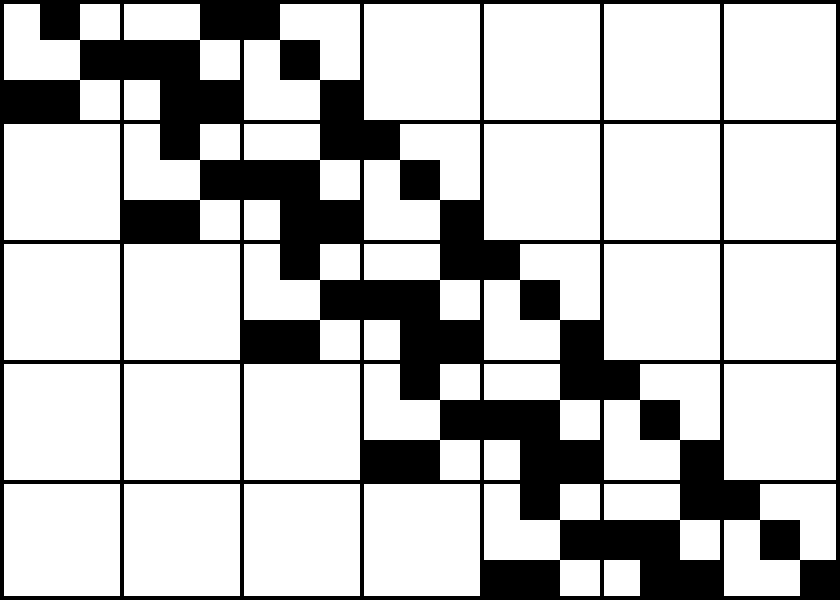
\includegraphics[width=12cm]{GRAPHICS/RS/RS_8_red_2_draw}
$$
\caption{\label{fig:RS:field:reduction}Field reduction of a Reed-Solomon code}
\end{figure}
Let us compute the weight enumerator of the reduced code.
The command 
{\tt
\input GRAPHICS/THE_MAKEFILE/EXTRACTS/RS_8_reduced.tex
}
{\tt
\input GRAPHICS/THE_MAKEFILE/EXTRACTS/RREF_RS_8_reduced_weight_enumerator.tex
}
computes the weight enumerator of the binary code. It is
$$
\begin{array}{p{12cm}}
$1y^{21} + 28x^3y^{18} + 84x^4y^{17} + 273x^5y^{16} + 924x^6y^{15} + 1956x^7y^{14} + 2982x^8y^{13} + 4340x^9y^{12} + 5796x^{10}y^{11} + 5796x^{11}y^{10} + 4340x^{12}y^9 + 2982x^{13}y^8 + 1956x^{14}y^7 + 924x^{15}y^6 + 273x^{16}y^5 + 84x^{17}y^4 + 28x^{18}y^3 + 1x^{21}$
\end{array}
$$
In particular, the field reduced Reed-Solomon code is not optimal. 
It has minimum distance three, but there are codes of minimum distance 4.
Here is one. We store the code to a file and then draw the generator matrix as bitmap.
{\tt
\input GRAPHICS/THE_MAKEFILE/EXTRACTS/CODE_21_15_4.tex
}
{\tt
\input GRAPHICS/THE_MAKEFILE/EXTRACTS/CODE_21_15_4_store.tex
}
We compute the weight enumerator
{\tt
\input GRAPHICS/THE_MAKEFILE/EXTRACTS/CODE_21_15_4_weight_enumerator.tex
}
which turns out to be
$$
\begin{array}{p{12cm}}
$1y^{21} + 221x^4y^{17} + 1600x^6y^{15} + 6498x^8y^{13} + 10912x^{10}y^{11} + 9250x^{12}y^9 + 3584x^{14}y^7 + 669x^{16}y^5 + 32x^{18}y^3 + 1x^{20}y.$
\end{array}
$$
This shows that this code is a $[21,15,4]_2.$ It is optimal.



In coding theory, one main question is 
to determine the best value of $d_{\max}$ for a fixed $n$, $k$ and $q$ such that 
a linear $[n,k,d]_q$ code exists.
There are many bounds, both upper and lower bounds. An upper bound tells us that no code with $d \ge d_{\max}$ exists.
A lower bound tells us that a code with $d \ge d_{\max}$ exists. 
The command  
{\tt
\input GRAPHICS/THE_MAKEFILE/EXTRACTS/bounds_for_d_given_n15_k6_q2.tex
}
gives upper and lower bounds on the optimal minimum distance $d_{max}$ of a $[15,6]_2$ code.
The values of the Gilbert-Varshamov lower bound and the Singleton, Hamming, Plotkin and Griesmer upper bounds are computed. 
The output is:
\begin{verbatim}
d_GV = 5
d_singleton = 10
d_hamming = 6
d_plotkin = 7
d_griesmer = 6
\end{verbatim}
This shows that $5 \le d_{\max} \le 6.$
The command 
{\tt
\input GRAPHICS/THE_MAKEFILE/EXTRACTS/coding_theory_bounds_q2.tex
}
produces a table of bounds for binary codes with $n,k \le 20.$
A file 
$$
\verb'table_of_bounds_n20_q2.csv'
$$ 
is computed.
The command 
{\tt
\input GRAPHICS/THE_MAKEFILE/EXTRACTS/GV_n15_k6_d5.tex
}
creates a $[15,6,d]_2$ with minimum distance $g \ge 5$ 
using a greedy algorithm based on the proof of the Gilbert-Varshamov bound.
The code that is produced has the following generator matrix:
\begin{verbatim}
1 1 1 1 1 1 1 1 1 1 0 0 0 0 0 
1 1 1 1 1 0 0 0 0 0 1 0 0 0 0 
1 1 1 0 0 1 1 0 0 0 0 1 0 0 0 
1 1 0 1 0 1 0 1 0 0 0 0 1 0 0 
1 0 1 0 1 0 1 1 0 0 0 0 0 1 0 
1 0 1 1 0 1 0 0 1 0 0 0 0 0 1 
\end{verbatim}
To compute the  minimum distance of the code, we do:
{\tt
\input GRAPHICS/THE_MAKEFILE/EXTRACTS/CODE_GV_N15_K6.tex
}
{\tt
\input GRAPHICS/THE_MAKEFILE/EXTRACTS/GV_n15_k6_d5_weight_enumerator.tex
}
The weight enumerator is
$$
1y^{15} + 27x^6y^9 + 24x^8y^7 + 9x^{10}y^5 + 3x^{12}y^3.
$$
From this, we see that the code has minimum distance $6,$ 
which is better than predicted.
%# surprise: d = 6

\bigskip
The classification problem of optimal codes 
in coding theory is the problem of determining the 
equivalence classes of codes for a given set of values 
of $n$ and $k$ and $q$ with a lower bound on $d.$ 
Orbiter can be used to classify linear codes with given redundancy and bounded minimum distance. 
The redundancy of a linear $[n,k]$ code is the parameter $r = n - k.$
Codes with redundancy $r$ can be identified with subsets of $\PG(r-1,q).$
Under this correspondence, 
a code with minimum distance at least $d$ corresponds to a subset such that any $d-1$ elements are independent.
We use the notation  $\Lambda_{r-1,s}(q)$ to denote the poset of 
subsets of $\PG(r-1,q)$ for which any $d-1$-subset (if any) is independent. 
Under the correspondence, 
the action of $\PGGL(r,q)$ on $\Lambda_{r-1,s}(q)$ corresponds to the orbits of equivalent linear codes.
For this reason, we are interested in determining the orbits of $\PGGL(r,q)$ on $\Lambda_{r-1,s}(q).$ 
An orbit of size $n$ represents an isometry class of  $[n,n-r,d;q]$ codes with $d \ge s +1.$
The projective stabilizer of the subset is the automorphism group of the code.
The Orbiter command 
{\tt
\input GRAPHICS/THE_MAKEFILE/EXTRACTS/codes_8_4_4.tex
}
classifies linear codes with redundancy $4$ and minimum distance at least $4$. 
Orbiter confirms that there is exactly one such code, and it 
computes the code together with the projective stabilizer.
Orbiter creates the action of 
the group $\PGL(4,2)$ on the poset $\Lambda_{3,3}(2).$ 
Using poset classification, Orbiter then produces the 
poset of orbits shown in Figure~\ref{fig:codes844}.
\begin{figure}
$$

\includegraphics[width=15cm]{GRAPHICS/codes_8_4_4}
$$
\caption{\label{fig:codes844}Orbits of $\PGL(4,2)$ on the poset $\Lambda_{3,3}(2)$}
\end{figure}
In this diagram, the numbers stand for Orbiter ranks of points in $\PG(3,2).$ 
All nodes except for the root node have a number attached to it.
The nodes represent subsets. In order to determine the set associated to a node, 
follow the path from the root node to the node and collect the points according to their labels. 
The root node represents the empty set.
The $[8,4,4;2]$-code is represented by the set $\{0,1,2,3,8,11,13,14\}.$
The fact that there is only one node at level $8$ 
in the poset of orbits tells us that the code is unique up to equivalence.
Let us look at the code. The elements of the set $\{0,1,2,3,8,11,13,14\}$
are points in $\PG(3,2)$. 
We write the coordinate vectors in the columns of a matrix $H$:
$$
H=\left[
\begin{array}{cccccccc}
1&0&0&0&1&1&1&0\\
0&1&0&0&1&1&0&1\\
0&0&1&0&1&0&1&1\\
0&0&0&1&0&1&1&1\\
\end{array}
\right].
$$
This matrix is the parity check matrix $H$ of the code $\cC.$
This means that the words of the code are the vectors $\bc$ such that $\bc\cdot H^\top = 0.$
Observe that the vectors that we put in the columns of $H$ all have odd weight. 
They are in fact the points of the hyperplane $x+y+z+w = 0.$ 
This shows that the stabilizer of the code which is the stabilizer of the set is 
equal to $\AGL(3,2)$, a group of order $1344.$

\bigskip
\section{Introduction}
\label{sec:combinatorics:intro}


\input C11/sec_1.tex

\bigskip


\clearpage


\section{Diophantine Systems}
\label{sec:diophant}


\input C11/sec_2.tex

\bigskip


\clearpage

\section{Combinatorial Linear Spaces}
\label{sec:combinatorial:linear:spaces}


\input C11/sec_3.tex

\bigskip


\clearpage


\section{Classification of Configurations and Geometries}
\label{sec:configurations}


\input C11/sec_4.tex

\bigskip


\clearpage


\section{Design Theory}
\label{sec:design}




\input C11/sec_5.tex




\bigskip
\clearpage

\section{Design Theory -- Large Sets}
\label{sec:large:sets}




\input C11/sec_6.tex




\bigskip
\clearpage
\section{Design Theory -- Delandtsheer-Doyen}
\label{sec:design:DD}




\input C11/sec_7.tex




\bigskip
\clearpage


\section{Tactical Decompositions}
\label{sec:tactical:decompositions}



\input C11/sec_8.tex




\bigskip
\clearpage

In Tables~\ref{tab:combi} and~\ref{tab:combi:2},  
global Orbiter commands for Combinatorics are summarized.
\begin{table}
	\begin{center}
	\begin{tabular}{|p{4cm}|p{3cm}|p{7cm}|}
		\hline
		Command & Arguments & Purpose \\
		\hline
		\hline
		\verb'-random_permutation' &  $n$ fname & Crates a random permutation in $\Sym(n)$ and stores it in the given file.\\
		\hline
		\verb'-create_random' \verb'_k_subsets' & $n$ $k$ $N$  & Creates $N$ random $k$-subsets of an $n$-set. \\
		\hline
		\verb'-read_poset_file' & fname  & Reads a poset from the given file. \\
		\hline
		\verb'-read_poset_file' \verb'_with_grouping' & fname x-stretch  & Reads a poset from the given file and sets stretch factor for orbit grouping. \\
		\hline
		\verb'-list_parameters' \verb'_of_SRG' &  $v_{\max}$ & Performs a sift for putative parameter sets of SRGs. \\
		\hline
		\verb'-conjugacy_classes' \verb'_Sym_n' & $n$  & Compute a list of conjugacy classes of $\Sym(n).$ \\
		\hline
		\verb'-tree_of_all' \verb'_k_subsets' & $n$ $k$  & Creates a tree-file for all $k$-subsets of an $n$-set. \\
		\hline
		\verb'-Delandtsheer_Doyen' &   & See Section~\ref{sec:design:DD}. \\
		\hline
		\verb'-tdo_refinement' &   & See Section~\ref{sec:tactical:decompositions}. \\
		\hline
		\verb'-tdo_print' &   & See Section~\ref{sec:tactical:decompositions}. \\
		\hline
		\verb'-convert_stack' \verb'_to_tdo' &   & See Section~\ref{sec:tactical:decompositions}. \\
		\hline
		\verb'-maximal_arc' \verb'_parameters' &   & See Section~\ref{sec:tactical:decompositions}. \\
		\hline
		\verb'-arc_parameters' &   & See Section~\ref{sec:tactical:decompositions}. \\
		\hline
		\verb'-pentomino_puzzle' &   &  \\
		\hline
		\end{tabular}
	\end{center}
	\caption{\label{tab:combi}Commands related to Combinatorics (Part 1)}
	\end{table}
\begin{table}
	\begin{center}
	\begin{tabular}{|p{4cm}|p{3cm}|p{7cm}|}
		\hline
		Command & Arguments & Purpose \\
		\hline
		\hline
		\verb'-draw_layered_graph' &  options & Draws a graph. \\
		\hline
		\verb'-make_elementary_' \verb'symmetric_functions' & $n$ $k_{\max}$ & Computes the elementary symmetric functions in $n$ 
		variables of degree $1, \ldots, k_{\max}$\\
		\hline
		\verb'-Dedekind_numbers' & $n_{\min}$  $n_{\max}$ $q_{\min}$  $q_{\max}$ & Computes the Dedekind numbers $D_{n,q}$ 
		for $n_{\min} \le n \le n_{\max}$ and $q_{\min} \le q \le q_{\max}$\\
		\hline
		\verb'-rank_k_subset' & $n$ $k$ $L$  & Computes the ranks of $k$-subsets chosen from an $n$-set. $L$ is a list of $k$-sets taken from an $n$-set. \\
		\hline
		\verb'-geometry_builder' &   & See Section~\ref{sec:configurations}.\\
		\hline
		\verb'-character_table_' \verb'symmetric_group' & $n$  & Computes the character table of  $\Sym(n)$ using the algorithm of Burnside. \\
		\hline
		\verb'-domino_portrait' & $D$ $s$ fname  & Computes a domino portrait for a graphics file in r/g/b format using double $D$ domino sets. \\
		\hline
		\end{tabular}
	\end{center}
	\caption{\label{tab:combi:2}Commands related to Combinatorics (Part 2)}
	\end{table}

\bigskip

The command 
{\tt
\input GRAPHICS/THE_MAKEFILE/EXTRACTS/Sym_10_conj_classes.tex
}
produces a list of the conjugacy classes of $\Sym(10).$ The list is written to a csv file. 
A pie chart 
of the class size distribution is shown in Fig.~\ref{fig:sym:10:classes}.
\begin{figure}
$$
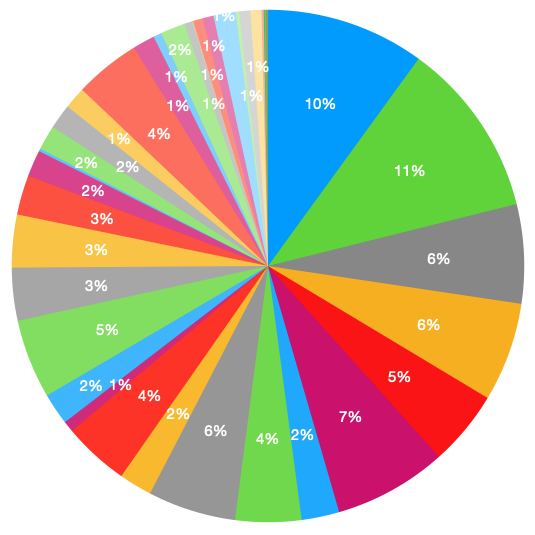
\includegraphics[width=10cm]{GRAPHICS/GROUPS/classes_Sym_10}
$$
\caption{\label{fig:sym:10:classes}The conjugacy classes of $\Sym(10)$ arranged by size}
\end{figure}


\bigskip


The next command computes the character table of the symmetric group $\Sym(4)$:
{\tt
\input GRAPHICS/THE_MAKEFILE/EXTRACTS/Char_Sym_4.tex
}
The command produces the following output:
\begin{mdframed}[style=MyFrame]
\input GRAPHICS/LATEX/character_table_sym_4.tex
\end{mdframed}

\bigskip

The following command creates the character table of $\Sym(4)$.
{\tt
\input GRAPHICS/THE_MAKEFILE/EXTRACTS/Char_Sym_4.tex
}


\bigskip

The following command illustrates how to create random $k$-subsets of a set of size $n$.
In the example, we create $20$ $5$-subsets of a $10$-element set:
{\tt
\input GRAPHICS/THE_MAKEFILE/EXTRACTS/random_k_subsets.tex
}


\bigskip

Using the lexicographic order, the $k$-subsets of an $n$-element set are ranked.
The following command computes the ranks of a number of $3$-subsets of a $10$-element set:
{\tt
\input GRAPHICS/THE_MAKEFILE/EXTRACTS/rank_k_subsets_test.tex
}


\bigskip

Orbiter can create the Sylvester type Hadamard matrix of size $2^n$ (also called the Walsh matrix). 
The following command creates the matrix of size $2^4 \times 2^4$ and produces a graphical representation:
{\tt
\input GRAPHICS/THE_MAKEFILE/EXTRACTS/Walsh_matrix_4.tex
}


\bigskip

The following command creates the matrix of Dedekind numbers of order at most 10:
{\tt
\input GRAPHICS/THE_MAKEFILE/EXTRACTS/Dedekind_10_10.tex
}


\bigskip




The following command creates the elementary symmetric functions in $4$ variables.
{\tt
\input GRAPHICS/THE_MAKEFILE/EXTRACTS/elementary_symmetric_functions_4.tex
}
The output is:
\begin{verbatim}
k=1 : 
x0 + x1 + x2 + x3
k=2 : 
x0*x1 + x0*x2 + x0*x3 + x1*x2 + x1*x3 + x2*x3
k=3 : 
x0*x1*x2 + x0*x1*x3 + x0*x2*x3 + x1*x2*x3
k=4 : 
x0*x1*x2*x3
\end{verbatim}

\bigskip

Orbiter can compute domino portraits. 
To do so, we need an input file in r/g/b format 
of size $(D+1)s \times Ds,$ where $D=7$ for double-six dominos.
{\tt
\input GRAPHICS/THE_MAKEFILE/EXTRACTS/domino_portrait.tex
}
The portrait is shown in Figure~\ref{fig:domino:portrait}. 
\begin{figure}
$$
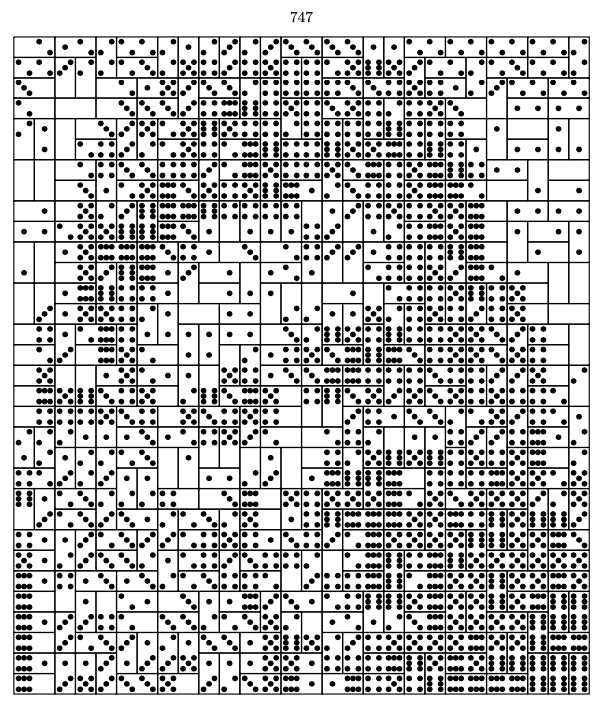
\includegraphics[width=10cm]{GRAPHICS/DOMINO/anton_domino}
$$
\caption{\label{fig:domino:portrait}Domino Portrait}
\end{figure}
It is possible to compare the domino portrait with a grayscale verson of the input image.
The following command creates a grayscale image of the input file 
that was written during the previous command.
{\tt
\input GRAPHICS/THE_MAKEFILE/EXTRACTS/domino_portrait_input.tex
}
The grayscale version of the input file is shown in Figure~\ref{fig:domino:grayscale}. 
\begin{figure}
$$
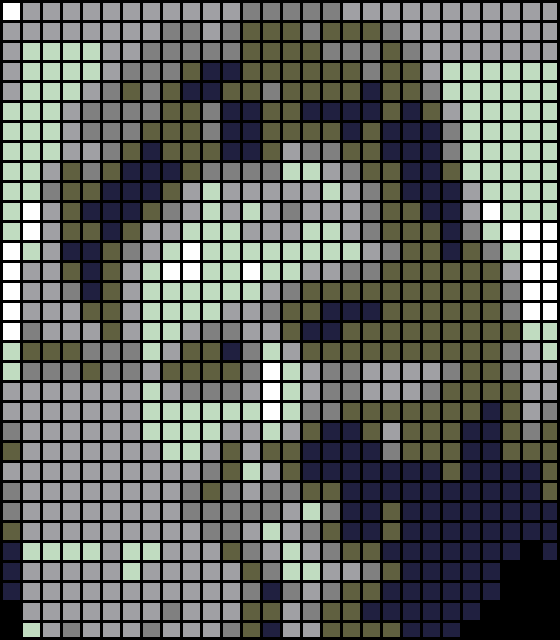
\includegraphics[width=8cm]{GRAPHICS/DOMINO/anton_28x32_m_draw}
$$
\caption{\label{fig:domino:grayscale}Domino portrait input file in grayscale}
\end{figure}




\bigskip


Diophantine systems of equations and inequalities arise frequently in Combinatorics.
In Table~\ref{tab:diophant}, Orbiter commands for creating and solving diophantine systems are shown.
\begin{table}
	\begin{center}
	\begin{tabular}{|p{4cm}|p{3cm}|p{7cm}|}
		\hline
		Command & Arguments & Purpose \\
		\hline
		\hline
		\verb'-label' & label & Use the given name as file name. \\
		\hline
		\verb'-coefficient_' \verb'matrix' & A  & Set the coefficient matrix to the previously created vector with format information. \\
		\hline
		\verb'-coefficient_' \verb'matrix_csv' & fname  & Read the coefficient matrix from the given csv-file.\\
		\hline
		\verb'-RHS' & list-of-integers  & $3n$ values: (RHS-low, RHS-high, RHS-type) for each row of the system.\\
		\hline
		\verb'-RHS_csv' & fname  & Read the RHS information from the given csv file.\\
		\hline
		\verb'-RHS_constant' & low,high,type  & Set the RHS according to low,high,type.\\
		\hline
		\verb'-x_max_global' & $a$  & Set the upper bound for all variables to $a$ \\
		\hline
		\verb'-x_min_global' & $a$  & Set the lower bound for all variables to $a$ \\
		\hline
		\verb'-x_bounds' & list-of-values  & Set the lower and upper bounds for all variables. \\
		\hline
		\verb'-x_bounds_csv' & fname  & Read the lower and upper bounds for all variables from the given file. \\
		\hline
		\verb'-has_sum' & $s$  & For the sum of the variables to be $s.$ \\
		\hline
		\verb'-maximal_arc' & $s$ $d$ secants subset & Create system for a maximal arc of size $s$ and degree $d$ in $\PG(2,q)$. Use the given set of two pencil lines. The subset picks the lines from the given pencils which are external.  \\
		\hline
		\verb'-q' & $q$  & Use $\PG(2,q)$ for maximal arcs. \\
		\hline
		\verb'-override_' \verb'polynomial' & $a$  & Use polynomial numerically coded as $a$ for creating $\bbF_q.$ \\
		\hline
		\end{tabular}
	\end{center}
	\caption{\label{tab:diophant}Orbiter Commands to create Diophantine systems}
	\end{table}
In Table~\ref{tab:diophant:activities}, Orbiter activities for diophantine systems are shown.
\begin{table}
	\begin{center}
	\begin{tabular}{|p{4cm}|p{3cm}|p{7cm}|}
		\hline
		Command & Arguments & Purpose \\
		\hline
		\hline
		\verb'-print' &  & Print the system. \\
		\hline
		\verb'-solve_mckay' &  & Solve the system using McKay's possolve.\\
		\hline
		\verb'-solve_DLX' &  & Solve the system using Knuth's dancing links.\\
		\hline
		\verb'-solve_standard' &  & Solve the system using the standard solver.\\
		\hline
		\verb'-draw' &  & Produce a drawing of the coefficient matrix of the system.\\
		\hline
		\verb'-draw_as_bitmap' & $w$ $b$ & Produce a bitmap 
		drawing of the coefficient matrix of the system, 
		using boxes of $w$ pixels with. 
		Set the color bit-depth to $b$ ($b=8$ or $b=24$). The output is a bmp-file. \\
		\hline
		\verb'-perform_' \verb'column_reductions' &  & 
		Eliminate variables which must be zero and write a reduced system.\\
		\hline
		\verb'-test_single' \verb'_equation' &  & For each row of the system, 
		compute the number of solutions of the system restricted to the nonzero coefficients. \\
		\hline
		\verb'-project_to_' \verb'single_equation' \verb'_and_solve' & $i$ $j$ & 
		Solve the system assuming the $j$th solution to the 
		restricted system consisting of the $i$th row. \\
		\hline
		\verb'-project_to_' \verb'two_equations' \verb'_and_solve' & $i$ $j$ $r$ $m$ & 
		Solve the system assuming any solution to the restricted system consisting of the $i$th 
		and the $j$-th row  whose number is congruent to $r$ mod $m$. \\
		\hline
		\end{tabular}
	\end{center}
	\caption{\label{tab:diophant:activities}Orbiter activities for Diophantine systems}
	\end{table}


Consider the matrix 
$$
A= 
\left[
\begin{array}{cccccc}
0&1&0&1&0&0\\
0&0&1&0&1&0\\
1&0&1&0&0&0\\
0&1&0&1&0&1\\
1&0&0&0&0&1\\
1&0&1&0&0&0\\
0&1&0&0&1&1\\
\end{array}
\right]
$$
Suppose we want to find all column vectors $\bx$ with entries in $0,1$ such that 
$$
A \bx = \bone
$$
where $\bone$ is the all-one column vector.
Orbiter offers two algorithms to do this. 
One is McKay's possolve, the other is Knuth's dancing links (DLX).
In order to get started, we need to create a diophant object.
In the following example, we use the makefile variable \verb'TEST_SYSTEM' for the 
coefficient matrix and \verb'TEST_RHS' for the right hand side.
{\tt
\input GRAPHICS/THE_MAKEFILE/EXTRACTS/TEST_SYSTEM.tex
}
{\tt
\input GRAPHICS/THE_MAKEFILE/EXTRACTS/TEST_RHS.tex
}
{\tt
\input GRAPHICS/THE_MAKEFILE/EXTRACTS/solve_test_system.tex
}

There are two commands to solve a diophantine system: \verb'-solve_mckay' and \verb'-solve_DLX'. The latter is more restrictive, 
as it allows only 0,1 variables.
Here is the McKay solver:
{\tt
\input GRAPHICS/THE_MAKEFILE/EXTRACTS/McKay_test.tex
}
The solutions are written to the file \verb'DLX_test.sol'. 
And now the dancing links solver:
{\tt
\input GRAPHICS/THE_MAKEFILE/EXTRACTS/DLX_test.tex
}


\bigskip


A linear space is a pair $(S,\cL)$ where $S$ is a set and $\cL$ is a set of subsets of $S$ such that 
each set $L \in \cL$ satisfies $|L| \ge 2$ and 
morover for any two $a,b \in S$ there is exactly one element $L \in \cL$
such that both $a$ and $b$ belong to $L.$ 
The usual notions of isomorphism and automorphism apply.
For finite linear spaces, a first combinatorial property is the number $a_i$ 
which counts the number of sets $L \in \cL$ of size $i.$ 
The vector $(a_2,\ldots,a_n)$ is the line type of $(S,\cL)$.
The equation 
\begin{equation}\label{eqn:linetype}
{n \choose 2} = \sum_{j=2}^n a_j {j \choose 2}
\end{equation}
is satisfied. 
The equation 
can be used to generate all possible line types of a putative linear space.
Here is an example. For $|S| = 6,$~(\ref{eqn:linetype}) becomes
$$
x_0 {6 \choose 2} + x_1 {5 \choose 2} + x_2 {4 \choose 2} + x_3 {3 \choose 2} + x_4 {2 \choose 2} = {6 \choose 2}.
$$
Here, $(x_0,x_1,\ldots,x_4)$ is the line type of a putative linear space on $6$ points. 
That is, $x_i = a_{6-i}$ is the number of lines of size $6-i.$
The extended coefficient matrix of the system is 
$$
\left[ 
15 \; 
10 \; 
6 \; 
3 \; 
1 \; 
\mid 
15 
\;
\right].
$$
The Orbiter command
{\tt
\input GRAPHICS/THE_MAKEFILE/EXTRACTS/linsp6.tex
}
solves the system using  McKay's program possolve~\cite{Possolve}. 
The program finds 15 solutions, written to the file \verb'linsp6.sol'.


\bigskip

Let us consider a problem from~\cite{BettenBetten10}.
Suppose we are interested in linear spaces on 30 points.
with line type $(7,5^{27},4^{24})$. 
This notation means that we assume 
one $7$-line, $27$ $5$-lines and $24$ $4$-lines. 
The type of a point $P$ is the set of integers 
$$
p_{j} = \# j\mbox{-lines though $P$}.
$$
We are trying to precompute the matrix of point types  
$$
(p_{ij})
$$
where $j=7,5,4$ and $i$ belongs to an index set of all possible point types.
Fixing a point $P$, counting points $Q \neq P$ collinear with $P$ yields
$$
6p_7 + 4p_5+3p_4 = 29, \quad p_7 \le 1, \; p_5 \le 27, p_4 \le 24.
$$
Using the Orbiter commands 
{\tt
\input GRAPHICS/THE_MAKEFILE/EXTRACTS/linsp30_pt_types.tex
}
we determine the possibilities 
$$
(p_7,p_5,p_4) = \left\{
\begin{array}{ccc}
1 & 5 & 1 \\
1 & 2 & 5 \\
0 & 5 & 3 \\
0 & 2 & 7 \\
\end{array}
\right.
$$
The rows in this matrix are called the point types $(i=0,1,2,3).$
Let $b_i$ be the number of points of type  $i.$
By counting points, incident (point,line) pairs by $j$-lines 
and pairs of intersecting $j$-lines, we arrive at the following system:
\begin{align*}
	b_0 + b_1 + b_2 + b_3 & = 30 \\
	b_0 + b_1 & = 7\\
	5b_0 + 2b_1 + 5b_2 + 2b_3 &= 135 = 27 \cdot 5\\
	b_0 + 5b_1+3b_2+7b_3 & = 96 = 24 \cdot 4\\
	10b_0 + b_1 + 10b_2 + b_3 & \le 351 = {27 \choose 2}\\
	10b_1+3b_2+21b_3 & \le 276 = {24 \choose 2}
\end{align*}
Using the Orbiter commands 
{\tt
\input GRAPHICS/THE_MAKEFILE/EXTRACTS/linsp30_pt_distribution.tex
}
we determine the possibilities 
$$
(b_0,b_1,b_2,b_3) = \left\{
\begin{array}{cccc}
2 &5 &23 &0 \\
3 &4 &22 &1 \\
4 &3 &21 &2 \\
5 &2 &20 &3 \\
6 &1 &19 &4 \\
7 &0 &18 &5 \\
\end{array}
\right.
$$
A partial linear space is a set system on a fixed set $V$. 
We write $\cL=(V,\cB),$ where $\cB$ is a set of distinct subsets of $V$, called lines. 
The members of $V \cup \cB$ are called elements. 
For two elements $x,y$, we say that $x$ is incident with $y$, written $xIy$, 
if either $x \in y$ or $y \in x.$
We require that any line has at least two points 
and any two points are contained in at most one line. 
A {\em decomposition} of a linear space is a partition $\Pi= (C_1,\ldots,C_n)$ of $V \cup \cB$ 
such that each $C_i$ either is a subset of $V$ or a subset of $\cB.$
A decomposition is called {\em tactical} if for all $i,$ the incidence number 
$$
\iota(C_i,C_j) = \# \{y \in C_j, xIy\}
$$
does not depend on the choice of $x \in C_i.$
Any linear space has a tactical decomposition, 
as the discrete partition (every element is in its own class) 
is tactical. 
Let $\Aut(\cL)$ be the automorphism group of the linear space, which is the subgroup of 
$\Sym(V)$ which preserves incidence. 
For $\alpha \in \Aut(\cL)$ we say that 
the decomposition $\Pi$ preserves $\alpha$ if $\alpha$ fixes every class of $\Pi.$ 
For $A \le  \Aut(\cL),$ we say that $\Pi$ preserves $A$ is $\Pi$ preseves every element $\alpha \in A.$
Mostly, we are interested in those decompositions $\Pi$ which preserve $\Aut(\cL).$
In light of this, the discrete decomposition is not that interesting. 

\bigskip


Any linear space has a coarsest tactical decomposition that preserves its automorphism group: 
The orbit partition of the automorphism group acting on $V \cup \cB$ will do. 
Up to ordering of the classes, the coarsest tactical refinement is unique.
Computing the orbit decomposition is challenging as it involves computing the automorphism group. 
Computationally, there are easier ways to get to admissible decompositions. 
One is by means of successive refinements. 
If a class $C_i$ does not have the property that $\iota(C_i,C_j)$ is well-defined 
for all $x \in C_i,$ then a refinement of $C_i$ will do. 
The coarsest refinement of $C_i$ has the property that 
if $C_i$ preserves some group $A$ then the refinement will do, too.
This shows that there is an algorithm to compute a tactical decompostion of any given linear space $\cP.$ 
Simply start with the decomposition of two classes, one the set of points and one the set of blocks, and refine. 
The output may or may not be equal to the decomposition arising from the orbit partition of $\Aut(\cL).$

\bigskip

Let us consider the opposite question. 
Given a tactical decomposition, does there exist a linear space
whose coarsest tactical decomposition is the given one? 
If so, how many nonisomorphic partial linear spaces are there 
for a given tactical decomposition? 
in other words, we would like to classify the linear spaces which admit a given tactical decomposition.
The \verb'-geometry_builder' option can answer these kinds of questions. 
Table~\ref{tab:geometry:builder} shows the options for the geometry builder.
\begin{table}
	\begin{center}
	\begin{tabular}{|p{4cm}|p{3cm}|p{7cm}|}
		\hline
		Command & Arguments & Purpose \\
		\hline
		\hline
		\verb'-V' & part  & The initial partition of points (rows). \\
		\hline
		\verb'-B' & part & The initial partition of blocks (columns). \\
		\hline
		\verb'-TDO' & tdo & The initial row-tactical decomposition scheme. \\
		\hline
		\verb'-fuse' & fuse & The partition of row classes. \\
		\hline
		\verb'-girth_test' & $g$ & Require the girth of the collinearity graph to be at least $g$. \\
		\hline
		\verb'-lambda' & $\lambda$ & Set $\lambda$ for two-design test. Every pair of points lies in $\lambda$ blocks. \\
		\hline
		\verb'-find_square' &  &  Construct linear spaces. \\
		\hline
		\verb'-simple' &  & Construct simple designs (needs \verb'-lambda') \\
		\hline
		\verb'-search_tree' &  & Write a file containing the search tree (at the level of rows of the partial geometry). \\
		\hline
		\verb'-search_tree_flags' &  & Write a file containing the search tree (at the level of flags of the partial geometry). A flag is an incident point-block pair. \\
		\hline
		\verb'-orderly' &  & User orderly generation. \\
		\hline
		\verb'-special_test_' \verb'orderly' &  & Use a special test. This option only applies to orderly generation. \\
		\hline
		\verb'-split' & $l$ $r$ $m$ & Split the search tree. After $l$ lines, continue only cases congruent to $r$ modulo $m$. \\
		\hline
		\verb'-fname_GEO' & fname & Set the output file name base (no extension). \\
		\hline
		\verb'-output_to_' \verb'inc_file' &  & Set output to inc file.  \\
		\hline
		\verb'-output_to_' \verb'sage_file' &  & Set output to sage file. \\
		\hline
		\verb'-output_to_' \verb'blocks_file' &  & Set output to a file containing the blocks in coded form. \\
		\hline
		\verb'-output_to_' \verb'blocks_latex_file' &  & Set output to a file containing the blocks in latex. \\
		\hline
		\end{tabular}
	\end{center}
	\caption{\label{tab:geometry:builder}Orbiter commands to build geometries}
	\end{table}


\bigskip

The command 
{\tt
\input GRAPHICS/THE_MAKEFILE/EXTRACTS/geo_10_3.tex
}
classifies the configuations $10_3$. 
It uses isomorphism tests after $4,$ $5,$ $6,$ $7,$ $8,$ $9$ and $10$ points.
The positions of the tests is defined using a set called \verb'Test_lines'. 
The set of test lines is defined using a loop command.
The command shows that 
there are exactly 10 configurations of this kind. 
One of them is the Desargues configuration. 
Four different output files can be written.
Each contains all geometries, but the file format is different.
\begin{enumerate}
\item
The option \verb'-output_to_inc_file'
writes \verb'10_3.inc'. 
The file contains the incidences in increasing order. 
The position in the incidence matrix is given.
One linear space is given per row, except for the first row and the last. 
The first row contains the number of points, the number of lines, and the number of incidences.
The incidences are given in numeric form. 
The last row start with $-1.$
Each incidence is the numerical position of the point/block pair in the 
incidence matrix. 
The position is the numbering of the matrix entries 
in the incidence matrix in row-major ordering, 
starting with zero for the top left entry. 
The index of the incidence in row $i$ (zero-based) and column $j$  is $b\cdot i + j,$ 
where $b$ is the number of blocks in the geometry.
In this case, with $b=10,$ zero represents the incidence between point 0 and block zero. 
The number 99 represents the incidence between point 9 and block 9.
Here is the file \verb'10_3.inc':

{\scriptsize
\begin{verbatim}
10 10 30
0 1 2 10 13 14 20 25 26 31 33 35 41 44 47 52 53 58 62 66 69 74 78 79 85 87 89 96 97 98 
0 1 2 10 13 14 20 25 26 31 33 35 41 44 47 52 54 58 62 66 69 73 78 79 85 87 89 96 97 98 
0 1 2 10 13 14 20 25 26 31 33 35 41 44 47 52 54 58 62 67 69 73 76 79 85 88 89 96 97 98 
0 1 2 10 13 14 20 25 26 31 33 35 41 44 47 52 56 58 62 67 69 73 78 79 84 86 89 95 97 98 
0 1 2 10 13 14 20 25 26 31 33 35 41 47 48 52 54 57 62 66 68 73 77 79 84 86 89 95 98 99 
0 1 2 10 13 14 20 25 26 31 33 35 41 47 48 52 54 57 62 66 68 73 78 79 84 86 89 95 97 99 
0 1 2 10 13 14 20 25 26 31 33 35 41 47 48 52 54 57 62 66 69 73 78 79 84 86 88 95 97 99 
0 1 2 10 13 14 20 25 26 31 33 37 41 45 48 52 54 57 62 66 68 73 75 79 84 86 89 97 98 99 
0 1 2 10 13 14 20 25 26 31 33 37 41 45 48 52 54 57 62 66 68 73 75 79 84 88 89 96 97 99 
0 1 2 10 13 14 20 25 26 31 33 37 41 45 48 52 54 57 62 66 68 73 76 79 84 88 89 95 97 99 
-1 10
120, 24, 12, 10, 6, 4^2, 3^2, 2
\end{verbatim}}
\item
The option \verb'-output_to_sage_file'
writes \verb'10_3.sage'. 
This file is meant to be read by Sage~\cite{SteinJoyner2005}.
\item
The option \verb'-output_to_blocks_file'
writes \verb'10_3.blocks'. 
Here is the content of the file \verb'10_3.blocks':
\begin{verbatim}
10 10 3
0 15 26 44 51 68 81 109 114 116 
0 15 26 46 49 68 81 109 114 116 
0 15 26 46 49 68 83 106 115 116 
0 15 26 46 52 69 77 106 114 116 
0 15 26 46 56 69 80 101 106 119 
0 15 26 46 56 69 80 103 104 119 
0 15 26 46 56 69 80 103 107 117 
0 15 26 46 56 72 80 93 106 119 
0 15 26 46 56 72 81 93 105 119 
0 15 26 46 56 74 79 93 105 119 
-1 10
120, 24, 12, 10, 6, 4^2, 3^2, 2
\end{verbatim}
contains the blocks. 
Each number represents the rank of a 3-subset corresponding to a block 
in the lexicographic ordering of all 3-subsets. 
\item
The option \verb'-output_to_blocks_latex_file'
writes \verb'10_3.blocks_long'. 
The file 
\verb'10_3.blocks_long' contains a list of all blocks written out in a format ready for use in latex.
\end{enumerate}

\bigskip

It is possible to create graphical representations of the search tree. 
The command below does so for the example that we just did. 
Note the additional option \verb'-search_tree'. 
This option causes Orbiter to create a file containing the search tree. 
The name of the file is derived from the file name given with the \verb'fname_GEO' option. 
Here, the \verb'fname_GEO' option sets the output file to \verb'10_3'. The \verb'-search_tree'
option then creates the file \verb'10_3_tree.txt'.
In a second invocation of Orbiter,
the \verb'-tree_draw' command is used to draw a tree 
from the file \verb'10_3_tree.txt' that was just created.
The vertex color represents the outcome of the isomorphism test. 
A green node is accepted. A red node is rejected. 
The search will continue for the green nodes only. 
A green node at the bottom of the tree corresponds 
to an isomorphism type of a geometry satisfying all the requirements. 
Here, the 10 green nodes at the very bottom 
of the diagram represent the 10 isomorphism types of configurations $10_3$.
{\tt
\input GRAPHICS/THE_MAKEFILE/EXTRACTS/geo_10_3_tree.tex
}
The size of the tree can be determined by counting the lines of the file \verb'10_3_tree.txt' and subtracting one:
\begin{verbatim}
wc 10_3_tree.txt
\end{verbatim}
The word count command yields the following output:
\begin{verbatim}
    1471   13543   37633 10_3_tree.txt
\end{verbatim}
This means that there are 1471 lines in the file. 
Hence the search tree has 1470 nodes.
The resulting tree is shown in Figure~\ref{fig:geo:10:3:tree}.
\begin{figure}
%\begin{mdframed}[style=MyFrame]
$$
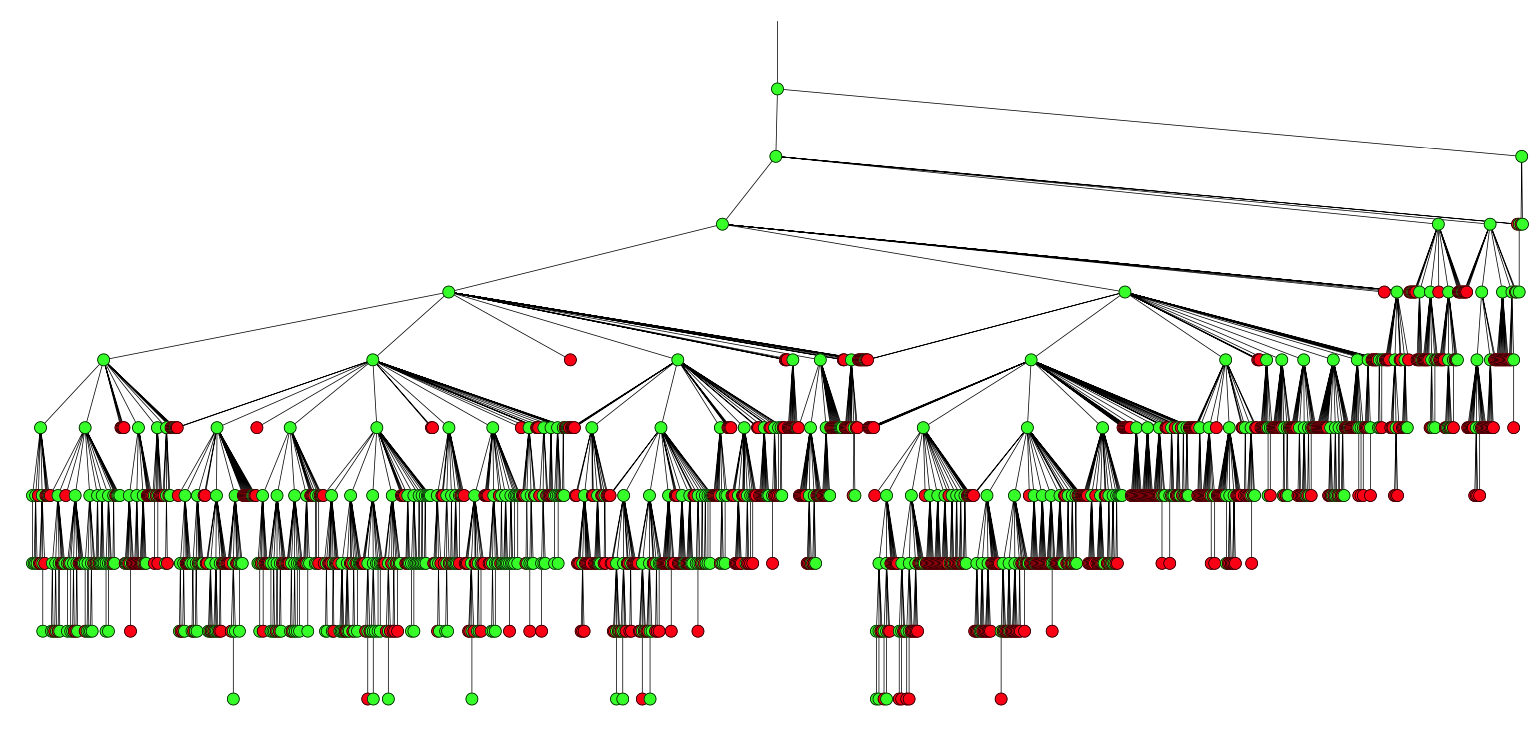
\includegraphics[width=15cm]{GRAPHICS/CONF/search_tree_conf_10_3}
$$
%\end{mdframed}
\caption{\label{fig:geo:10:3:tree}Search tree for the classification of $10_3$ configurations}
\end{figure}

\bigskip


Any incidence structure defines a graph on its underlying set of points. 
The vertices are the points of the incidence structure.
Two vertices are adjacent if and only if the incidence structure contains a block 
which contains the associated points. 
In a geometric context, the graph is known as the collinearity graph of the geometry.
The distance between two points is the distance of the associated vertices in the collinearity graph. 
The girth is the length of the shortest cycle. 
It is often desired to classify incidence structures with a given girth.  
This means that we are given an integer $g$ (the girth), and that we are looking for incidence structures 
whose collinearity graph has no cycles of length less than $g.$
For instance, the following example classifies all cubic graphs on 10 vertices with girth at least 5:
{\tt
\input GRAPHICS/THE_MAKEFILE/EXTRACTS/geo_petersen.tex
}
There is a unique graph with these properties. 
It is the Petersen graph. 
Its automorphism group is $\Sym(5)$ of order $120.$

\bigskip

We can classify configurations with a given girth. 
For instance, while there are $245342$ isomorphism classes of configurations $15_3$, 
only one of them has girth 4. This is the Cremona Richmond configuration. 
It is associated to a cubic surface.
The following command classifies all configurations $15_3$:
{\tt
\input GRAPHICS/THE_MAKEFILE/EXTRACTS/15_3.inc.tex
}
This command takes about 8 minutes of time to complete.

\bigskip


The next command classifies the configurations $15_3$ with girth $4.$ 
Only one configuration arises, 
the Cremona Richmond, with automorphism group $\Sym(6)$ of order 720. 
{\tt
\input GRAPHICS/THE_MAKEFILE/EXTRACTS/geo_15_3_g4.tex
}

\bigskip


The next command classifies the configurations $40_4$ with girth $4.$ 
Exactly two configuration arise, both with a group of order 51840. 
Note the extra option \verb'-special_test_not_orderly' to speed up the search.
{\tt
\input GRAPHICS/THE_MAKEFILE/EXTRACTS/40_4_g4.inc.tex
}
The search tree is shown in Figure~\ref{fig:40:4:search:tree}.
\begin{figure}
$$
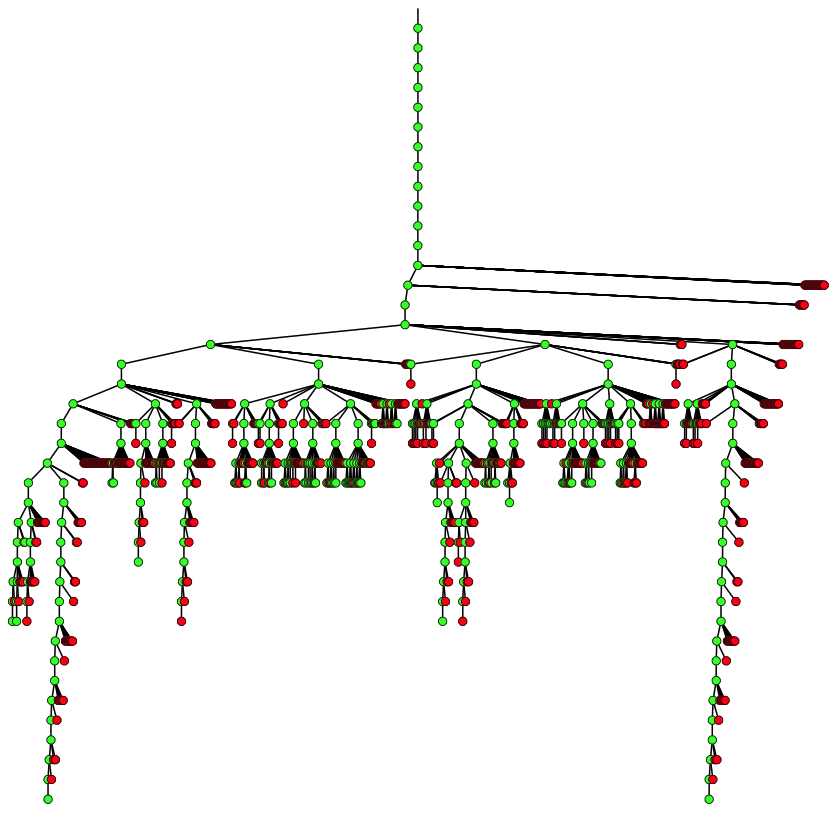
\includegraphics[width=15cm]{GRAPHICS/CONF/search_tree_conf_40_4_g4}
$$
\caption{\label{fig:40:4:search:tree}The search tree for the configurations $40_4$ with girth $4$}
\end{figure}


\bigskip

The next command classifies the configurations $63_3$ with girth $6.$ 
Exactly two configuration arise, both with a group of order 12096. 
Note the extra option \verb'-special_test_orderly' to speed up the search.
{\tt
\input GRAPHICS/THE_MAKEFILE/EXTRACTS/geo_63_3_g6.tex
}
The search tree is much larger than for the previous problem.


\bigskip



A design is an incidence structure of points and blocks. 
The incidence matrix of a design has rows corresponding to the points 
and columns corresponding to the blocks. 
An entry in a certain row and column is one if and only if the point associated with the row 
is contaned in the block associated with the column, zero otherwise.
A decomposition of the design is a partition of the points and blocks such that 
each class consists either exclusively of points or exclusively of blocks. 

\bigskip


A decomposition is point-tactical if for all points, 
the number of incident lines in the $j$th block class depends only on the class of the point.
It the point belongs to class $i,$ this number is denoted as $a_{ij}.$
A decomposition is block-tactical if for all blocks, 
the number of incident points in the $i$th point class depends only on the class of the block.
If the block belongs to class $j,$ this number is denoted as $b_{ij}.$

\bigskip

A projective plane of order $n$ is a 
design with $n^2+n+1$ points and equally many blocks (also called lines), each of size $n+1$ such that 
any two points lie in exactly one block and any two blocks have exactly one point in common.
Projective planes are known to exist for all $n = q$ which are a power of a prime. 
This follows from a construction which utilizes the projective geometry $\PG(2,q).$ 
Points are the one-dimensional subspaces of $\bbF_q^3,$
blocks are the two-dimensional subspaces of $\bbF_q^3,$ and
incidence is natural (inclusion of subspaces). 
The automorphism group of this design is the collineation group of the projective space.
Projective planes other than these exist, though none are known when $n$ is not a prime power.
The number of lines through a point equals the number of points on a line. 
The fact that these numbers exist imply that there is a tactical decomposition. 
Namely, the trivial decomposition with two classes, one containing all points and one containing all lines.
The structure constants of the decomposition are the numbers just described.

\bigskip

The command 
{\tt
\input GRAPHICS/THE_MAKEFILE/EXTRACTS/design_PG_2_3.tex
}
creates the design $\PG(2,3).$ 
\begin{mdframed}[style=MyFrame]
\input GRAPHICS/LATEX/design_PG_2_3.tex
\end{mdframed}
The blocks of the design are encoded in the lexicographic ordering of $k$-subsets (here $k=4$)
The program also displays the tactical decomposition schemes of the design, which are
\begin{mdframed}[style=MyFrame]
\input GRAPHICS/LATEX/design_PG_2_3_td.tex
\end{mdframed}
In Section~\ref{sec:canonical:form:objects:design:theory}, we will show how to compute 
further properties of the design.


\bigskip

The command 
{\tt
\input GRAPHICS/THE_MAKEFILE/EXTRACTS/wreath_product_designs_n4_k2_inc.txt.tex
}
creates a design on $8$ points invariant under the wreath product $\Sym(4) \wr \Sym(2).$
The design has 12 blocks of size 4. 
The command 
{\tt
\input GRAPHICS/THE_MAKEFILE/EXTRACTS/wreath_product_designs_n8_k6_inc.txt.tex
}
creates a design on $16$ points invariant under the wreath product $\Sym(8) \wr \Sym(2).$
The design has 3920 blocks of size 6. 
We will compute the automorphism groups of these two designs in Section~\ref{sec:canonical:form:objects:incidence:geometries}.


\bigskip

One way to construct designs is by assuming a suitable group of symmetries. 
Let us consider an example. 
It is possible to construct $t$-$(v,k,\lambda)$ designs invariant under a permutation group $G$ 
acting on a set $V$ with $|V| = v$ as follows: 
Classify the orbits of $G$ on subsets of size $k$ and less. 
Construct a matrix which describes the relationship between the orbits on $t$-sets and the orbits on $k$-sets. 
This matrix is often referred to as the Kramer-Mesner matrix (cf.~\cite{KramerMesner76}).
For each pair of $t$-orbit and $k$-orbit, for instance with representatives $T$ and $K$, say, 
we count the number of elements in the orbit of $K$ which contain $T$. 
The rows of the matrix are in correspondence to the $t$-orbits, while the columns are in correspondence to the $k$-orbits. 
The matrix entry $a_{ij}$ is the number just defined where $T$ is the representative of the 
$i$-th orbit on $t$-sets,  and where $K$ is the representative of the $j$-th orbit on $k$-sets. 
Let $M_{t,k}(G)$ be the Kramer-Mesner matrix 
for the group $G \le \Sym(V)$ defined in this way. 
The 
$t$-$(v,k,\lambda)$ designs invariant under $G$ are in one-to-one correspondence to the solutions of 
$$
M_{t,k}(G)\cdot \bx = \lambda {\bf 1},
$$
where $\bx$ is a column vector of zeros and ones and ${\bf 1}$ is the column vector of all ones.
The length of $\bx$ is the number of $k$-orbits of $G$ on $V$, 
while the length of $\bone$ is the number of $t$-orbits of $G$ on $V$. 
Any vector $\bx$ satisfying the matrix equation corresponds to a design invariant under $G$.
Simply take the  blocks of the design to be the union of those orbits of $G$ on $k$-subsets 
whose associated entry in $\bx$ is one.
We assume the group $\PGGL(2,32)$ in the action on points of the projective line $\PG(1,32)$ 
over the field $\bbF_{32}.$
The parameters of the design are $7$-$(33,8,10)$, that is, each $7$-subset of $\PG(1,32)$
is covered exactly 10 times by the chosen $8$-subsets comprising the design.
The first orbiter command creates the group $\PGGL(2,32)$ and computes the Kramer-Mesner matrix 
$$
M_{7,8}(\PGGL(2,32)).
$$
The number of $7$-orbits is 32. The number of $8$-orbits is $97.$
Correspondingly, the Kramer-Menser matrix has 32 rows and 97 columns.
The matrix is stored in the csv-file 
$$
\verb'KM_PGGL_2_32_KM_7_8.csv'.
$$
The second command produces the graphical representation of the matrix shown in Figure~\ref{fig:KMPGGL} 
\begin{figure}
$$

\includegraphics[width=15cm]{GRAPHICS/KM_PGGL_2_32_KM_7_8_draw}
$$
\caption{\label{fig:KMPGGL}Kramer-Mesner matrix $M_{7,8}(\PGGL(2,32))$}
\end{figure}
(different colors represent different values of entries in the matrix).
The third Orbiter command creates the diophantine system associated with the Kramer-Mesner matrix. 
{\tt
\input GRAPHICS/THE_MAKEFILE/EXTRACTS/KM_PGGL_2_32.tex
}
The last command performs a complete enumeration of all solutions by solving the system and producing 
the solution vectors $\bx$ 
which correspond to the designs. 
Fix a set of size $v$ and an integer $k$ with $1 <k < v.$ Is it possible to partition the set of 
$k$-subsets of $v$ into designs, all with the same parameters? 
If so, the resulting set of designs is called a large set (of designs).
So, a large set of designs is a set of designs, all of the same types, 
on a fixed $v$-element set 
whose block sets are pairwise disjoint and partition the set of 
$k$-subsets. 
Let us see how Orbiter can help construct and classify small large sets.


\bigskip

Suppose we consider $\AG(2,3)$, the affine plane of order 3. 
It is a configuration with 9 points, 12 lines, 4 lines on each point and 3 points on each line.
To see if it is unique, we use the following command:
{\tt
\input GRAPHICS/THE_MAKEFILE/EXTRACTS/AG_2_3.inc.tex
}
The command produces the file \verb'AG_2_3.inc', which contains the following lines:
{\scriptsize
\begin{verbatim}
9 12 36
0 1 2 3 12 16 17 18 24 31 32 33 37 40 43 46 49 53 56 59 62 64 69 71 74 78 80 82 87 89 93 94 99 102 103 107 
-1 1
432
\end{verbatim}}
This shows that the design is unique, and has an automorphism group of order $432$.
For the following commnds, we will treat blocks of the design as sets of ranks of $k$-subsets. 
We can now create a table of all designs $\AG(2,3),$ as orbit under the group $\Sym(9).$
The following command does that:
{\tt
\input GRAPHICS/THE_MAKEFILE/EXTRACTS/AG_2_3_BLOCKS.tex
}
{\tt
\input GRAPHICS/THE_MAKEFILE/EXTRACTS/LS_AG_2_3_design_table_create.tex
}
The number of designs is $|\Sym(9)|/432 = 362880/432 = 840.$
To find all large sets, we establish the block-disjointness graph 
on this set of designs. After that, we find all cliques of size 7:
{\tt
\input GRAPHICS/THE_MAKEFILE/EXTRACTS/LS_AG_2_3_disjoint_sets_graph_and_cliques.tex
}
The files \verb'AG_2_3_design_table_disjoint_sets_sol.txt' and \verb'AG_2_3_design_table_disjoint_sets_sol.csv' are created, each containing the cliques of size 7. 
There are exactly 15360 cliques of size 7.
It remains to classify the resulting 15360 large sets up to isomorphism. 
To do that, we first need to create the actual large sets from the cliques.
The following command does that:
{\tt
\input GRAPHICS/THE_MAKEFILE/EXTRACTS/LS_AG_2_3_export_solutions.tex
}
The final step to classify the large sets up to isomorphism 
will be discussed in Section~\ref{sec:canonical:form:objects:design:theory}.



Delandtsheer and Doyen in~\cite{DelandtsheerDoyen1989} study 
line-transitive and point-imprimitive designs 
and show that they are rare in a certain sense.
Orbiter can be used to construct such designs 
assuming that there is a grid structure on the set 
of points and assuming that the design is invariant under a chosen group $G$. 
The group $G$ is assumed to be a subgroup of the group 
$\AGL(d_1,q_1) \times \AGL(d_2,q_2)$ acting on a grid of size 
$q_1^{d_1} \times a_2^{d_2}$ in product action.

\bigskip

Finite projective planes often arise in this context. 
However, not all examples are projective planes. Orter can help to classify small examples.
Let us consider an example. 
Suppose we want to classify all designs on 21 points with blocks of size $k=5$ 
invariant under a cyclic group of order $21$ preserving a grid of type $3 \times 7.$ 
To this end, we consider the group $\AGL(1,3) \times \AGL(1,7).$ 
The subgroup is generated by the map
$$
(\tau_1,\tau_2), \bbZ_3 \times \bbZ_7 \rightarrow  \bbZ_3 \times \bbZ_7,
$$ 
where 
$$
\tau_1: \bbZ_3 \rightarrow \bbZ_3, \; x \mapsto x+1 \mod 3,
\quad
\tau_2: \bbZ_7 \rightarrow \bbZ_7, \; y \mapsto y+1 \mod 7.
$$
With blocks of size 5, we cover $10$ pairs each. 
The group of order 21 allows to cover each of the $210={21\choose 2}$ pairs 
exactly once using a single orbit of a block.
The question remains to construct all blocks and to classify the resulting designs.
The Desarguesian plane $\PG(2,4)$ provides a solution. 
The question is to decide whether there are any other, nonisomorphic designs.
The following Orbiter commands can be used:
{\tt
\input GRAPHICS/THE_MAKEFILE/EXTRACTS/PP4.tex
}
{\tt
\input GRAPHICS/THE_MAKEFILE/EXTRACTS/PP4_GROUP1.tex
}
{\tt
\input GRAPHICS/THE_MAKEFILE/EXTRACTS/PP4_MASK1.tex
}
The command \verb'DD_PP4' sets up the orbits of the group 
on pairs and writes the file \verb'PP4_pair_covering.csv'.
{\tt
\input GRAPHICS/THE_MAKEFILE/EXTRACTS/DD_PP4.tex
}
The command \verb'DD_PP4_system' creates a diophantine system of Steiner type
and solves it. 
{\tt
\input GRAPHICS/THE_MAKEFILE/EXTRACTS/DD_PP4_system.tex
}
It finds exacly one solution. 
This must be the $\PG(2,4)$ design.
Since there are no more designs, isomorphism testing is not needed.

%# 18603 = 27 * 53 * 13

Table~\ref{tab:tdo:refine} lists the Orbiter commands for decomposition refinement.
\begin{table}
	\begin{center}
	\begin{tabular}{|p{4cm}|p{3cm}|p{7cm}|}
		\hline
		Command & Arguments & Purpose \\
		\hline
		\hline
		\verb'-lambda3' & $\lambda_3$ $s$ &  Refine as 3-design with $\lambda_3$ and with block-size $s$  \\
		\hline
		\verb'-solution' & $i$ fname  &  Use solutions to system $i$ from file fname. \\
		\hline
		\verb'-range' & $f$ $l$  & Refine cases $i$ with $f \le i < f + l$ only.   \\
		\hline
		\verb'-select' & label   &  Select the case for refinement by label.  \\
		\hline
		\verb'-o1' &  $s$ & Omit $s$ variables from the first refinement system.   \\
		\hline
		\verb'-o2' & $s$  &  Omit $s$ variables from the second refinement system.   \\
		\hline
		\verb'-D1_upper_bound_x0' &  $b$ &  Add the bound $x_0\le b$ in the first refinement. \\
		\hline
		\verb'-reverse' &   & Sort the distributions in reverse order.   \\
		\hline
		\verb'-reverse_inverse' &   &    \\
		\hline
		\verb'-nopacking' &   &  Do not use packing inequalities.  \\
		\hline
		\verb'-dual_is_' \verb'linear_space' &   &  Assume that the dual incidence structure is a linear space also. This is valid for projective planes, for instance.  \\
		\hline
		\verb'-geometric_test' &   &  Subject the distributions to the geometric test.  \\
		\hline
		\verb'-once' &   &  Find at most one refinement in each case. This can be used to test which cases can be refined. \\
		\hline
		\verb'-mckay' &   &  Use McKay's solver instead (by default, a lexicographic solver is used).  \\
		\hline
		\verb'-input_file' & fname  &  Specify the input TDO-file for refinement.  \\
		\hline
		\end{tabular}
	\end{center}
	\caption{\label{tab:tdo:refine}TDO refinement options}
	\end{table}

\bigskip

Suppose we want to study projective planes of order $16.$ 
It is a linear space with $16^2+16+1=273$ points and equally many lines. 
Each point lies on $17$ lines and each line contains $17$ points. 
Any two points lie on exactly one line and any two lines intersect in exactly one point.

\bigskip

We decide to 
study maximal arcs of degree $4$ in this plane (the degree has to divide the order of the plane).
A maximal arc of degree $d$ is a set of points so that each line intersects in either $d$ or zero points.
A line which intersects in $d$ points is called a secant.  
A line which intersects in no point is called an external line.
The command 
{\tt
\input GRAPHICS/THE_MAKEFILE/EXTRACTS/max_arc_16_4_start.tex
}
creates a decomposition stack for the parameters of the arc and writes the file \verb'max_arc_q16_r4.stack' 
\begin{verbatim}
<HTDO type=pt ptanz=2 btanz=2 fuse=simple>
             221       52 
      52      17        0 
     221      13        4 

  1  1
</HTDO>
\end{verbatim}
This is a point-tactical decomposition with 2 point-classes and 2 block-classes. 
The point classes are associated with the rows. 
The block-classes are associated with the columns. 
The first row and column indicates the size of the classes.
The entries $a_{ij}$ count the number of blocks in the column class $j$ 
that are incident with a given point in the $i$th row  class.
The fuse information at the bottom (\verb'1 1') 
is a partition of the row classes which indicates the ancestor decomposition which was column tactical.
The next step is to convert the stack file to a tdo file.
The command
{\tt
\input GRAPHICS/THE_MAKEFILE/EXTRACTS/max_arc_16_4_convert_stack_tdo.tex
}
does that. 
It creates the file \verb'max_arc_q16_r4.tdo'. It also 
prints the decomposition stack:
\begin{verbatim}
lambda_scheme at level 2 : 
is 1 x 1
          | 273_{  1}
=====================
273_{  0} | 

row_scheme at level 4 : 
is 2 x 2
          | 221_{  1} 52_{  2}
==============================
 52_{  0} |        17        0
221_{  3} |        13        4

col_scheme at level 3 : 
is 1 x 2
          | 221_{  1} 52_{  2}
==============================
273_{  0} |        17       17
\end{verbatim}
Next, we can compute all coarsest column-tactical refinements of the decomposition. 
To this end, the command 
{\tt
\input GRAPHICS/THE_MAKEFILE/EXTRACTS/max_arc_16_4_refine.tex
}
is used. 
Because the incidence structure is a projective plane, the dual is a linear space also. 
Hence the option \verb'-dual_is_linear_space' can be used, which is helpful to reduce possibilities. 
As it turns out, there is exactly one refinement, and it is tactical. 
The file \verb'max_arc_q16_r4r.tdo' is produced. 
Note the added letter \verb'r' at the end of the file name (r for refinement).
We can use the following command to display the decomposition stack in the file:
{\tt
\input GRAPHICS/THE_MAKEFILE/EXTRACTS/max_arc_16_4r_print.tex
}
This produces the following output:
\begin{verbatim}
decomposition 0.1:
lambda_scheme at level 2 : 
is 1 x 1
          | 273_{  1}
=====================
273_{  0} | 

row_scheme at level 4 : 
is 2 x 2
          | 221_{  1} 52_{  2}
==============================
 52_{  0} |        17        0
221_{  3} |        13        4

col_scheme at level 4 : 
is 2 x 2
          | 221_{  1} 52_{  2}
==============================
 52_{  0} |         4        0
221_{  3} |        13       17

extra_col_scheme at level 3 : 
is 1 x 2
          | 221_{  1} 52_{  2}
==============================
273_{  0} |        17       17
\end{verbatim}


\section{Spreads}
\label{sec:spreads}

\input C12/sec_1.tex


\bigskip

\clearpage


\section{Translation Planes}
\label{sec:translation:planes}

\input C12/sec_2.tex


\bigskip

\clearpage


\section{Packings}
\label{sec:packings}

\input C12/sec_3.tex

	

\clearpage

\section{BLT-Sets}
\label{sec:BLT:sets}

\input C12/sec_4.tex

\clearpage



A $t$-spread of $\PG(n,q)$ is a set of disjoint $\PG(t,q)$ that cover all of $\PG(n,q)$ pointwise. 
$t$-spreads in $\PG(n,q)$ exist if and only if $t+1$ divides $n+1.$
In order to create a spread, Orbiter offers several commands, as summarized in Table~\ref{tab:spreads:define}.
\begin{table}
	\begin{center}
	\begin{tabular}{|p{4cm}|p{3cm}|p{7cm}|}
		\hline
		Command & Arguments & Purpose \\
		\hline
		\hline
		\verb'-kernel_field' & $F$ & Define the kernel of the spread. $F$ must be an object of type finite field.\\
		\hline
		\verb'-group' & $G$ & Define the group acting on the spread. Should be $\PGGL(2k,F)$. \\
		\hline
		\verb'-k' & $k$ & Set the dimension of the spread. \\
		\hline
		\verb'-catalogue' & $i$ & Pull spread number $i$ from the catalogue of spreads associated with the given field and the given dimension. \\
		\hline
		\verb'-family' & $L$ & Define a spread from a named family $L.$ So far, no family has been provided. \\
		\hline
		\verb'-spread_set' & $S$ & 
		Define a spread from the named spreadset $S$. 
		The spreadset $S$ must be a vector object. It must contain $q^3k^2$ entries over $F.$ \\
		\hline
		\end{tabular}
	\end{center}
	\caption{\label{tab:spreads:define}Orbiter commands to define a spread}
	\end{table}
The following two commands create the two spreads of order 9, relying on the Orbiter knowledge base.
{\tt
\input GRAPHICS/THE_MAKEFILE/EXTRACTS/create_spread_9a.tex
}
{\tt
\input GRAPHICS/THE_MAKEFILE/EXTRACTS/create_spread_9b.tex
}
The first spread is the Desarguesian spread, with automorphism group of order 5760.
The second spread is the Hall spread with automorphism group of order 1920.

\bigskip

Spreads can be defined using spread sets. 
A spread set is a set of $q^k$ matrices of size $k \times k$ over $\bbF_q$ such that $A_i-A_j$ 
is nonsingular for all $i \neq j.$ 
Let us look at an example. 
The spread due to Rao and Rao~\cite{RaoRao1976} 
can be defined using the following makefile variable. 
{\tt
\input GRAPHICS/THE_MAKEFILE/EXTRACTS/SPREAD_SET_27_RAO_RAO.tex
}
Each line represents one matrix of the spread set, with matrix entries being listed consecutively.
The following command can be used to define the spread:
{\tt
\input GRAPHICS/THE_MAKEFILE/EXTRACTS/create_spread_Rao_Rao_27.tex
}


%The reason is the existence of the Desarguesian spread (also called the regular spread). 
%The Desarguesian spread is created from $\PG(m-1,Q)$ where $Q = q^s$ for some integer $s.$ 
%The spread elements are the subspaces which arise by considering the elements of $\PG(m-1,Q)$ as vector %spaces over 
%$\bbF_q$. As such, they are rank $s$ subspaces in $\PG(n-1,q)$. 
%So, with $t = s-1$, we have a $t$-spread in $\PG(n-1,q)$. 

\bigskip


The following command creates the Desarguesian line-spread in $\PG(3,2)$: 
% (so $s=2,$ $t=s-1=1$, $m=2$, $q=2$, and $Q=4$):
{\tt
\input GRAPHICS/THE_MAKEFILE/EXTRACTS/desarguesian_spread_in_PG_3_2.tex
}
The cheat sheet contains the following spread:\\
\begin{mdframed}[style=MyFrame]
\input GRAPHICS/LATEX/desarguesian_spread_PG_3_2.tex
\end{mdframed}

\bigskip

The following command creates the Desarguesian plane-spread in $\PG(5,2)$:
{\tt
\input GRAPHICS/THE_MAKEFILE/EXTRACTS/desarguesian_spread_in_PG_5_2.tex
}
\begin{mdframed}[style=MyFrame]
\input GRAPHICS/LATEX/desarguesian_spread_PG_5_2.tex
\end{mdframed}

\bigskip



%Apart from the second spread element, 
%the left halves of the generator matrices of the subspaces in the Desarguesian spread 
%are the elements of $\bbF_8$ in a matrix representation over $\bbF_2$.

%\bigskip

Two $t$-spreads are isomorphic if there is a collineation which maps one to the other. 
The classification problem for $t$-spreads is the problem of determining a complete set of pairwise non-isomorphic 
$t$-spreads. The problem is computationally difficult. 
Orbiter can be used to classify spreads for small parameters. 
For greater classification power, the method of classification by substructure is used.
Let us look at some examples. 



\bigskip

At first, we look at an example which is sufficiently small and can be 
solved using the standard method. 
Here, the standard method is poset classification algorithm for partial spreads.
Suppose we want to classify the line spreads in $\PG(3,4)$ under the action of $\PGGL(4,4).$ 
Under the Andr\'e, Bruck-Bose construction~\cite{Andre54,BruckBose64}, 
these spreads correspond to translation planes of order $16$ with kernel $\bbF_4.$
In order to classify the spreads of $\PG(3,4)$, we use the command
{\tt
\input GRAPHICS/THE_MAKEFILE/EXTRACTS/classify_spreads_16_4.tex
}
The command uses poset classification to classify the spreads. 
To this end, it computes the poset of orbits for the group $G =\PGGL(4,4)$ acting on 
the poset of partial spreads in $\PG(3,4)$, 
shown in Figure~\ref{fig:spreads:16:4}.
\begin{figure}
$$
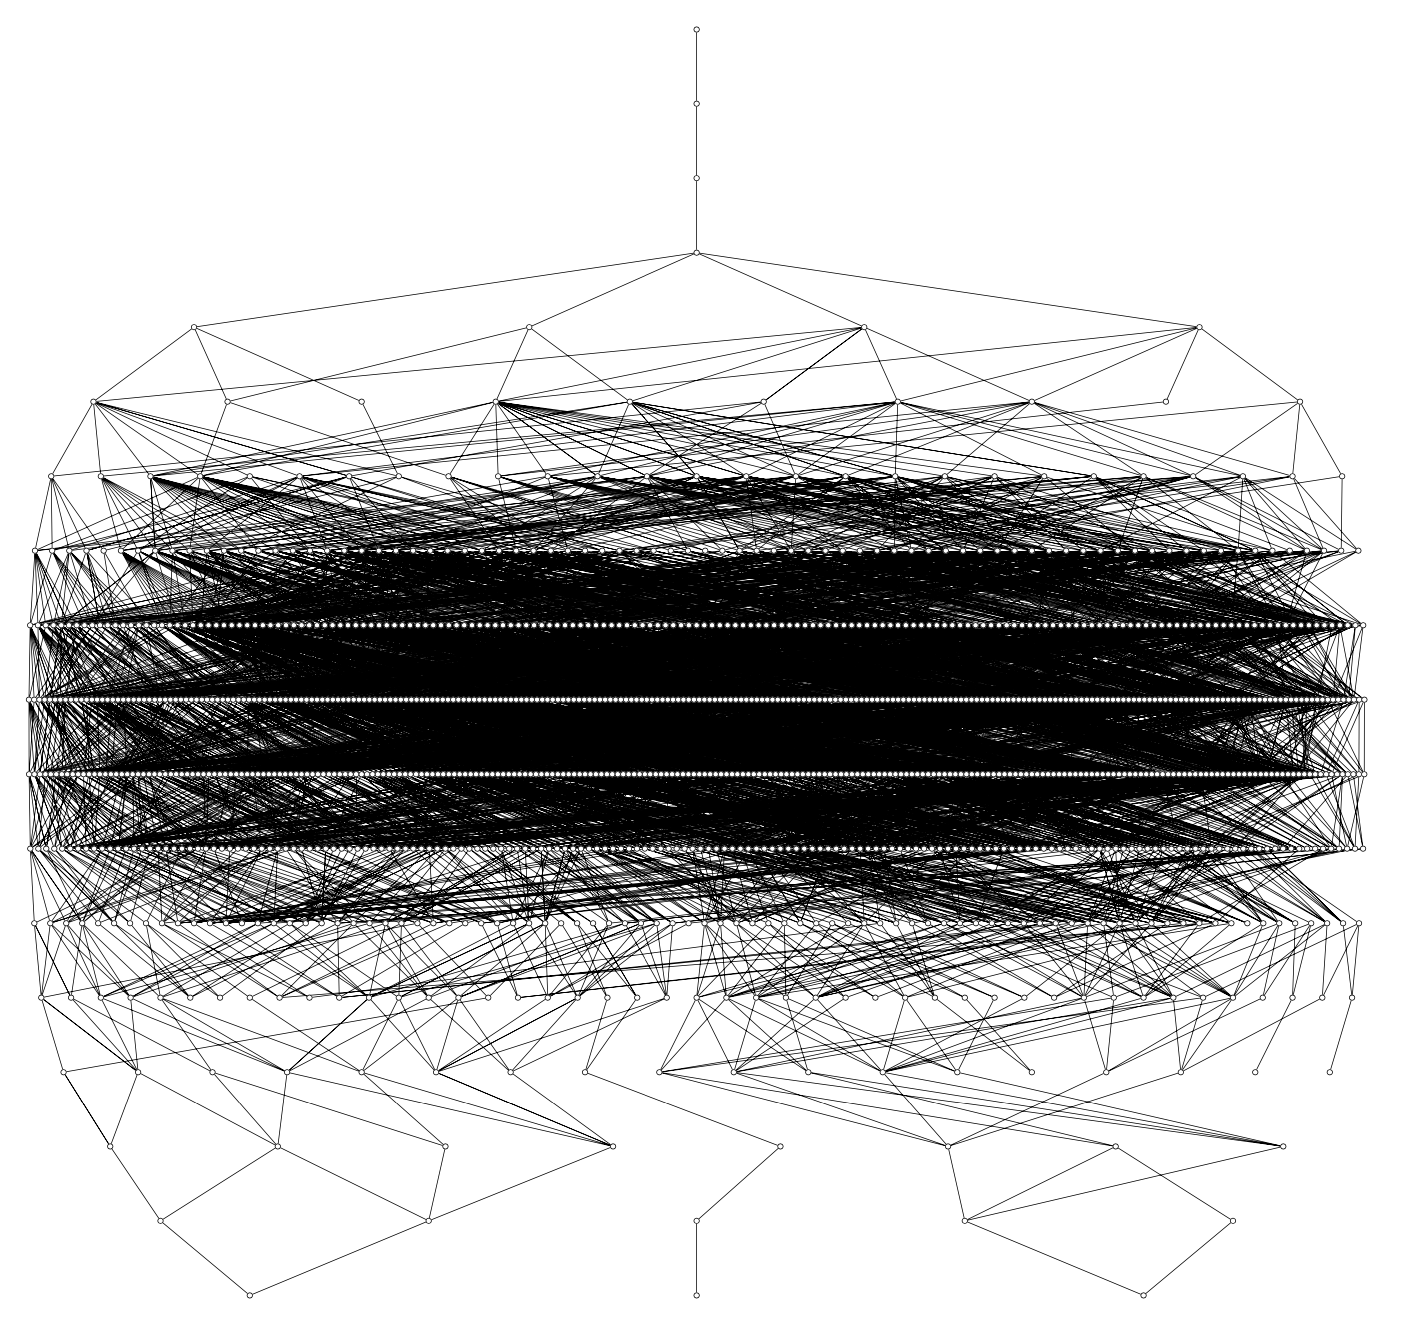
\includegraphics[width=16cm]{GRAPHICS/SPREADS/spreads_16_4}
$$
\caption{\label{fig:spreads:16:4}The poset of orbits of partial spreads in $PG(3,4)$}
\end{figure}
Up to isomorphism, there are exactly 
three line-spreads in $\PG(3,4)$ (corresponding 
to the three nodes at the bottom of the poset of orbits in the figure). 
These three spreads are the dearguesian spread, 
the Hall spread, and the semifield spread, respectively. 
Here is the relevant output taken from the latex report:
\begin{mdframed}[style=MyFrame]
\input GRAPHICS/LATEX/partial_spreads_PG_3_4.tex
\end{mdframed}
The three spreads in $\PG(3,4)$ can be distinguished by their stabilizer orders.
Table~\ref{tab:spreads:3:4} lists the line spreads in $\PG(3,4)$ according to their orbiter catalogue number (OCN).
\begin{table}
\begin{center}
\begin{tabular}{|r|c|r|}
\hline
OCN & $|\mbox{Aut}|$ & Name \\
\hline
0 & 1200 & Hall spread \\
1 & 81600 & Desarguesian spread \\
2 & 576 & Semifield spread\\
\hline
\end{tabular}
\end{center}
\caption{\label{tab:spreads:3:4}Spreads in $\PG(3,4)$  in the Orbiter Catalogue}
\end{table}


\bigskip

Let us now look at a more difficult problem. 
We wish to classify the spreads in $\PG(3,5).$
To this end, we will use the method of classification by substructure. 
We pick a size $s$ of a partial spread, and classify all partial spreads of size $s$. 
These are the substructures. 
Next, we perform the lifting, which means we construct all spreads of $\PG(3,5)$ 
containing one of the orbit representatives of the substructures. 
In a final step, we perform an isomorph classification on the set of liftings. 
This will furnish the desired classification of spreads of $\PG(3,5).$
From a computational point of view, the lifting process is the bottleneck in this procedure. 
Because of this, we use specialized algorithms from graph theory, which enhance the performance of the lifting. 
Specifically, we perform a search for rainbow cliques. 
We will go over some examples to illustrate the technique. 
To begin with, we choose the parameter $s=5.$

\bigskip


The command 
{\tt
\input GRAPHICS/THE_MAKEFILE/EXTRACTS/classify_spreads_25_starter_lift_case_0.tex
}
classifies the partial spreads of size $s=5$ and 
prepares for the lifting of the first case only. 
In order to prepare for the lifting, a graph is constructed which 
describes the lines that can be added to the first partial spread. 
The vertices of the graph are the lines disjoint from the initial set of 5 lines in the partial spread. Two vertices are joined by an edge of the associated lines are disjoint. 
The vertices of the graph are colored according to the very first basis vector in the 
generator matrix of the subspace in reduced row echelon form.
In order to find the rianbow clique in the graph, the command 
{\tt
\input GRAPHICS/THE_MAKEFILE/EXTRACTS/spreads_25_starter_0_cliques.tex
}
can be used. 

\bigskip

The command 
{\tt
\input GRAPHICS/THE_MAKEFILE/EXTRACTS/classify_spreads_25_starter_lift_all_cases.tex
}
recomputes the partial spreads of size $s=5$ and prepares for the lifting of all 
orbit representatives (there are 28). This leads to 28 graphs, each of which is 
written to a file.
The next command performs the rainbow clique finding in each of the 28 graphs:
{\tt
\input GRAPHICS/THE_MAKEFILE/EXTRACTS/spreads_25_starter_cliques.tex
}
The resulting cliques are again stored in files. 
The command 
{\tt
\input GRAPHICS/THE_MAKEFILE/EXTRACTS/classify_spreads_25_isomorph.tex
}
performs the final isomorph rejection on the spreads arising from the 
rainbow cliques in all cases. 
It results in a transversal of the isomorphism classes 
of spreads of $\PG(3,5).$ 
In total, 21 spreads are found. 
Of course, this agrees with the results in the literature, 
see~\cite{CzerwinskiOakden92}.






\bigskip




Table~\ref{tab:spreads:7:2} lists the solid spreads in $\PG(7,2)$ 
according to their Orbiter catalogue number (OCN).
\begin{table}
\begin{center}
\begin{tabular}{|r|c|r|}
\hline
OCN & $|\mbox{Aut}|$ & Name \\
\hline
0 & 1008 & \\
1 & 1008 & \\
2 & 1728 & \\
3 & 216 & \\
4 & 360 & \\
5 & 288 & \\
6 & 3600 & \\
7 & 244800 & \\
\hline
\end{tabular}
\end{center}
\caption{\label{tab:spreads:7:2}Spreads in $\PG(7,2)$ in the Orbiter Catalogue}
\end{table}



Orbiter can create translation planes from spreads. 
The construction of translation planes from spreads is due to Andr\'e and Bruck, Bose (cf.~\cite{Andre54,BruckBose64}). 
In order to perform the construction, we need a field $F=\bbF_q$ which is the kernel of the plane, 
a spread of $k$-subspaces, and the groups $\PGGL(2k,F)$ and $\PGGL(2k+1,F)$.
For instance, the command 
{\tt
\input GRAPHICS/THE_MAKEFILE/EXTRACTS/create_translation_plane_9b.tex
}
creates the (projective) Hall plane of order 9 from the Hall spread.
In this example, we use the fact that $\PGGL(n,q) = \PGL(n,q)$ if $q$ is prime.
The example also creates a bitmap drawing of the incidence matrix of the plane, shown in Figure~\ref{fig:plane:hall:9}.
\begin{figure}
$$
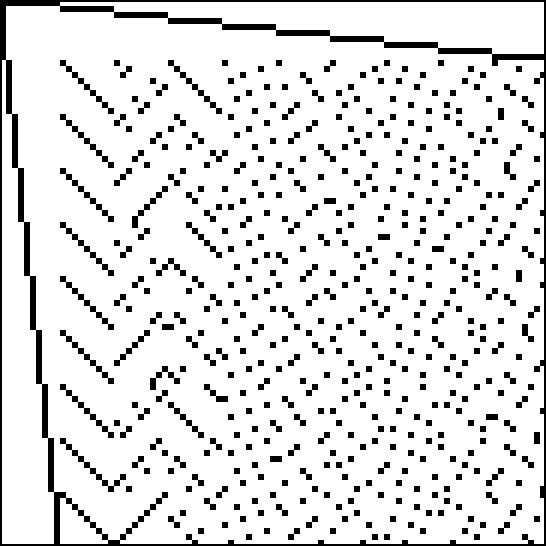
\includegraphics[width=11cm]{GRAPHICS/TRANSLATION_PLANES/plane_catalogue_q3_k2_1_incma_draw}
$$
\caption{\label{fig:plane:hall:9}Incidence matrix of the Hall plane of order 9}
\end{figure}

\bigskip

In the next example, we create a translation plane of order 16 with kernel of order 4:
{\tt
\input GRAPHICS/THE_MAKEFILE/EXTRACTS/create_translation_plane_16_4_0.tex
}
This plane is the Hall plane, and the spread is the Hall spread. 
The spread has a stabilizer of order 1200.

\bigskip

In the next example, we create a translation plane of order 16 with kernel of order 2:
{\tt
\input GRAPHICS/THE_MAKEFILE/EXTRACTS/create_translation_plane_16_2_0.tex
}
The spread has a stabilizer of order 1008, which means that the associated translation plane has a stabilizer of order $1008 \cdot 256 = 258045.$
According to~\cite{Moorhouse:tables:16}, there are two planes 
whose associated spreads have this automorphism group order. They can be distinguished by the 2-rank of their incidence matrices. 
The Johnson-Walker plane has a 2-rank of 100. 
The Lorimer-Rahilly plane has a 2-rank of 106. 
Using Orbiter, we compute the 2-rank of the translation plane that we have created:
{\tt
\input GRAPHICS/THE_MAKEFILE/EXTRACTS/RREF_plane_16_2_0_rank_of_incma.tex
}
It turns out that the 2-rank of our plane is 106, so the plane is Lorimer-Rahilly.


\bigskip

Let us investigate the Rao / Rao plane from Section~\ref{sec:spreads}, which we know is isomorphic to the spread in the Orbiter catalogue with number 0 and projective stabilizer of order 84.
The command  
{\tt
\input GRAPHICS/THE_MAKEFILE/EXTRACTS/create_translation_plane_27_Rao_Rao.tex
}
creates the translation plane from the spread 
(there is an error message which we can ignore; 
this is because we did not create the stabilizer of the spread).
To compute the 3-rank of the incidence matrix, we issue the following comand:
{\tt
\input GRAPHICS/THE_MAKEFILE/EXTRACTS/RREF_Rao_Rao_plane_incma_rank.tex
}
The 3-rank turns out to be 271. According to the Moorhouse tables~\cite{Moorhouse:tables:27}, 
the plane is Moorhouse IV.


A packing of $\PG(3,q)$ 
is a set of pairwise line-disjoint spreads of $\PG(3,q)$ of size $q^2+q+1.$ 
Each spread contains $q^2+1$ lines. 
A simple counting argument shows that 
every line is contained in exactly one spread of the packing.
The classification problem for packings 
is the problem of determining a complete set of pairwise non-isomorphic 
packings. 
Orbiter can be used to classify packings for small parameters. 
It is sometimes useful to make a symmetry assumption.
This means that only those packings will be found that satisfy the symmetry assumption. 
The reason for making such an assumption is that the problem becomes easier and hence more tractable.
Often, an assumption is made that the packings are invariant under a (nontrivial) group $H$.
This section describes various ways in which Orbiter can help find and classify packings, 
with or without symmetry assumption.

\bigskip


Table~\ref{tab:packings:was} list Orbiter commands related 
to the construction of packings with assumed symmetry.
\begin{table}
\begin{center}
\begin{tabular}{|p{5cm}|p{2cm}|p{7cm}|}
\hline
Command & Arguments & Purpose \\
\hline
\verb'-H' & description   & 
Specify the assumed group $H$ of symmetries. 
The orbits of $H$ on the set of spreads are considered. 
The packings will be constructed as union of orbits. \\
\hline
\verb'-N' & description   & Specify the normalizer of $H$.\\
\hline
%\verb'-spreads_invariant_' \verb'under_H' &    &  \\
%\hline
\verb'-cliques_on_' \verb'fixpoint_graph' &  $s$  & 
Using poset classification, 
classify the orbits of $N$ on cliques of size $\le s$ in the graph on fixed points. \\
\hline
\verb'-cliques_on_' \verb'fixpoint_graph_control' &  descr  & 
Specify poset classification options related to the classification 
of cliques on the fixed point graph as in Table~\ref{tab:pc:options}. \\
\hline
\verb'-fixp_clique_types_' \verb'save_individually' &    & 
Sort the cliques on fixed points by the type 
of their spreads and write one csv file for each possible 
type containing the index of the cliques of the given type.  \\
\hline
\verb'-process_long_orbits' &  descr  & 
Proceed on to long orbits using Table~\ref{tab:packings:long:orbits}. \\
\hline
%\verb'-problem_label' &  $L$  &  Use label $L$ within output file names. \\
%\hline
\verb'-spread_tables_prefix' &  $P$  &  Use prefix $P$ to access spread tables. \\
\hline
%\verb'-output_path' &  $P$  & Use prefix $P$ for output files. \\
%\hline
\verb'-report' &    & Create a report of the classification process. \\
\hline
\verb'-regular_packing' &    &  
Initialize Klein correspondence and identify (regular) 
spreads with external lines to the Klein quadric 
using the polarity of the Klein quadric. \\
\hline
\end{tabular}
\end{center}
\caption{\label{tab:packings:was}Orbiter commands related to the 
construction of packings with assumed symmetry}
\end{table}

\bigskip

Table~\ref{tab:packings:long:orbits} list Orbiter commands related to the construction 
of packings with assumed symmetry by picking long orbits.
\begin{table}
\begin{center}
\begin{tabular}{|p{5cm}|p{2cm}|p{7cm}|}
\hline
Command & Arguments & Purpose \\
\hline
\verb'-list_of_cases_' \verb'from_file' & fname   &  
Define a subset of cases of fixed point cliques to be worked on.  
Only the cases listed the given file are considered.  \\
\hline
\verb'-split' & $r$ $m$   & 
Define a subset of cases of fixed point cliques to be worked on. 
Only those cases whose number is congruent to $r$ modulo $m$ are considered. \\
\hline
\verb'-orbit_length' & $l$   &  Use orbits of length $l$. \\
\hline
\verb'-clique_size' &  $s$  & Use exactly $s$ orbits of length $l$. \\
\hline
\verb'-solution_path' &  $P$  &  Use $P$ as a prefix for all solution files. \\
\hline
\verb'-create_graphs' &    & 
For each case, create the graph that describes whether two orbits of length $l$ are compatible. \\
\hline
\verb'-solve' &    & 
Perform clique finding and write solutions to file. \\
\hline
\verb'-read_solutions' &    &  
Read solutions from file. \\
\hline
\end{tabular}
\end{center}
\caption{\label{tab:packings:long:orbits}Orbiter commands related to the construction 
of packings with assumed symmetry related to picking long orbits}
\end{table}


\bigskip

The following command creates a table of all labeled spreads in $\PG(3,4).$ 
There are three isomorphism types of spreads in $\PG(3,4)$. The command computes the orbits of each.
In total, this gives 5096448 labeled spreads. 
{\tt
\input GRAPHICS/THE_MAKEFILE/EXTRACTS/spread_table_PG_3_4.tex
}

\bigskip

There are 21 isomorphism types of spreads in $\PG(3,5).$ 
The regular spread has Orbiter catalogue number equal to 12. 
The following command creates a table of all labeled regular spreads:
{\tt
\input GRAPHICS/THE_MAKEFILE/EXTRACTS/spread_table_PG_3_4.tex
}
There are $155000$ regular spreads.




A BLT-set of $Q(4,q)$ is a set of $q+1$ point on the quadric 
such that no point on the quadric is collinear to more than two points of the set. 
BLT sets are related to spreads of $\PG(3,q),$ to flocks 
of the quadratic cone in $\PG(3,q)$, and to many other objects in combinatorics and finite geometry.
They exist whenever $q$ is odd. 
BLT-sets have been defined in~\cite{BaderLunardonThas90}.
It is an interesting problem to classify BLT-sets of $Q(4,q)$ under the orthogonal group.
Some references are 
Law~\cite{Law03}, Penttila-Royle~\cite{PenttilaRoyle98}, 
Penttila-Law~\cite{LawPenttila03,LawPenttila04}, 
Betten~\cite{Betten13}, AlAzemi-Betten-Chowdhury~\cite{AlAzemiBettenChowdhury18}.

\bigskip


Orbiter can be used to create members of known families of BLT-sets 
and sets from a catalogue of BLT-sets over small fields. 
Besides that, 
Orbiter can be used to classify all BLT-sets for a given value of $q$. 
We will see how we create known examples of BLT-sets either from the catalogue or from known families. 
Afterwards, we will consider the problem of classification.


\bigskip

Table~\ref{tab:BLT:create} shows options to create known BLT-sets.
\begin{table}
\begin{center}
\begin{tabular}{|p{4cm}|c|p{8cm}|}
\hline
Command & Arguments & Purpose \\
\hline
\hline
\verb'-catalogue' & $i$ & Create BLT-set number $i$ from the Orbiter catalogue ($i$ is zero-based). \\
\hline
\verb'-family' & $F$ & Create a BLT-set from family $F$. See Table~\ref{tab:BLT:families} for possibilities for $F$.\\
\hline
\end{tabular}
\end{center}
\caption{\label{tab:BLT:create}Commands for creating BLT-sets}
\end{table}
Table~\ref{tab:BLT:families} shows options for known families or sporadic sets.
\begin{table}
\begin{center}
\begin{tabular}{|p{4cm}|c|p{8cm}|}
\hline
Command & Condition & Purpose \\
\hline
\hline
\verb'Linear' &  & Linear BLT-set. \\
\hline
\verb'Fisher' &  & Fisher BLT-set~\cite{FisherThas79}. \\
\hline
\verb'Mondello' & $q \equiv \pm 1 \mod 10$ & Mondello BLT-set due to Penttila~\cite{Penttila98}. \\
\hline
\verb'FTWKB' & $q \equiv \pm 2 \mod 3$ & Fisher, Thas, Walker~\cite{Walker76}, Kantor, Betten~\cite{Betten73} BLT-set. \\
\hline
\verb'Kantor1' & $q=p^e, \; e > 1$ & Kantor's first family. \\
\hline
\verb'Kantor2' & $q \equiv \pm 2 \mod 5$ & Kantor's second family. \\
\hline
\verb'LP_37_72' & $q=37$ & BLT-set for $q=37$ with ago=72 due to Law and Penttila~\cite{LawPenttila04}. \\
\hline
\verb'LP_37_41a' & $q=37$  & First BLT-set for $q=37$ with ago=4, due to Law and Penttila~\cite{LawPenttila04}. \\
\hline
\verb'LP_37_41b' & $q=37$  & Second BLT-set for $q=37$ with ago=4, due to Law and Penttila~\cite{LawPenttila04}. \\
\hline
\verb'LP_71' & $q=71$  & BLT-set for $q=71$ due to Law and Penttila~\cite{LawPenttila04}. \\
\hline
\end{tabular}
\end{center}
\caption{\label{tab:BLT:families}Families of BLT-sets}
\end{table}
For instance, the command
{\tt
\input GRAPHICS/THE_MAKEFILE/EXTRACTS/BLT_11_0.tex
}
creates the BLT-set \#0 in $Q(4,11).$
The command
{\tt
\input GRAPHICS/THE_MAKEFILE/EXTRACTS/BLT_11_Mondello.tex
}
creates the Mondello BLT-set in $Q(4,11).$
Orbiter creates the following report:
\begin{mdframed}[style=MyFrame]
\input GRAPHICS/LATEX/BLT_mondello.tex
\end{mdframed}



\bigskip

The classification of BLT-sets is a difficult problem. 
For recent contributions, see~\cite{AlAzemiBettenChowdhury18,Betten13,Law03}.
One approach is by means of the poset of partial BLT-sets. 
The following command classifies the poset of partial BLT-sets in  $Q(4,13)$:
{\tt
\input GRAPHICS/THE_MAKEFILE/EXTRACTS/BLT_13_deep_search.tex
}
The poset of partial BLT-sets is too big, and there are too many orbits. 
The technique of classification via substructure can help. 
Here is an example. We consider the same problem of BLT-sets of order 13. 
In the beginning, we classify all partial BLT-sets 
of size $5$, and then create colored graphs for each 
of them: 
{\tt
\input GRAPHICS/THE_MAKEFILE/EXTRACTS/BLT_13_classify_starter.tex
}
In the next step, we compute all rainbow cliques in each of the graphs:
{\tt
\input GRAPHICS/THE_MAKEFILE/EXTRACTS/BLT_13_cliques.tex
}
Next, we create a data structure for isomorphism testing. 
The first step is to create a database of 
all partial BLT-sets of order at most 5:
{\tt
\input GRAPHICS/THE_MAKEFILE/EXTRACTS/BLT_13_isomorph_read_DB.tex
}
The next step is to read the rainbow cliques from the clique finding process:
{\tt
\input GRAPHICS/THE_MAKEFILE/EXTRACTS/BLT_13_isomorph_read_solutions.tex
}
Then, we compute the stabilizer orbits, which are also known as the flag orbits:
{\tt
\input GRAPHICS/THE_MAKEFILE/EXTRACTS/BLT_13_isomorph_stabilizer_orbits.tex
}
Finally, we perform isomorphism testing:
{\tt
\input GRAPHICS/THE_MAKEFILE/EXTRACTS/BLT_13_isomorph_testing.tex
}
This last command results in three isomorphism types of BLT-sets of order 13.



\section{Creating Graphs}
\label{sec:graphtheory}


\input C13/sec_1.tex



\bigskip


\clearpage


\section{Graph Theoretic Activities}
\label{sec:graph:theoretic:acivities}


\input C13/sec_2.tex



\bigskip


\clearpage

\section{Classification of Graphs and Tournaments}
\label{sec:graphtheory:classification}


\input C13/sec_3.tex



\bigskip


\clearpage


\section{Clique Finding}
\label{sec:graphtheory:cliques}


\input C13/sec_4.tex



\bigskip


\clearpage

Tables~\ref{tab:graphtypes:one}-\ref{tab:graphtypes:two} show Orbiter commands to create graphs.
\begin{table}
\begin{center}
\begin{tabular}{|p{4cm}|c|p{7cm}|}
\hline
Command & Arguments & Purpose \\
\hline
\hline
\verb'-load' & filename  & Read a graph from file in Orbiter format. \\
\hline
\verb'-load_csv_no_border' & filename  & Read a graph from a csv file. Ignore the first row and first column. \\
\hline
\verb'-load_dimacs' & filename  & Read a graph from file in dimacs format. \\
\hline
\verb'-edge_list' & $n$ list-of-edges  & Create a graph on $n$ vertices from a list of edges as ranked pairs. \\
\hline
\verb'-edges_as_pairs' & $n$ edges-as-pairs  & Create a graph on $n$ vertices from a list of edges as pairs. \\
\hline
\verb'-cycle' & $n$   & Cycle graph on $n$ vertices. \\
\hline
\verb'-Hamming' & $n$ $q$  & Hamming graph $H(n,q)$ \\
\hline
\verb'-Johnson' & $n$ $k$ $s$  & Johnson graph \\
\hline
\verb'-Paley' & $q$  & Paley graph \\
\hline
\verb'-Sarnak' & $p$ $q$  & Lubotzky-Phillips-Sarnak graph~\cite{Lubotzky1988} \\
\hline
\verb'-Schlaefli' & $q$  & Schlaefli graph \\
\hline
\verb'-Shrikhande' &   & Shrikhande graph \\
\hline
\verb'-Winnie_Li' & $q$ $i$  & Winnie-Li graph~\cite{Li1992} \\
\hline
\verb'-Grassmann' & $n$ $k$ $q$ $r$  & Grassmann graph \\
\hline
\verb'-coll_orthogonal' & $\epsilon$ $d$ $q$   & Collinearity graph of $O^\epsilon(d,q)$\\
\hline
\verb'-trihedral_pair_' \verb'disjointness_graph' &    & Triheral pair disjointness graph\\
\hline
\verb'-non_attacking_' \verb'queens_graph' &  $n$  & Create the graph for non-attacking queens 
on a $n \times n$ chess board. \\
\hline
\end{tabular}
\end{center}
\caption{\label{tab:graphtypes:one}Orbiter commands to define graphs (Part 1)}
\end{table}
\begin{table}
\begin{center}
\begin{tabular}{|p{4cm}|c|p{7cm}|}
\hline
Command & Arguments & Purpose \\
\hline
\hline
\verb'-subset' & label  labeltex subset  & Define vertex coloring with two colors based on a subset of vertices. \\
\hline
\verb'-disjoint_sets_' \verb'graph' & fname  & Define a graph on a system of sets. Adjacency is when two sets are disjoint. The sets are taken from the given file. \\
\hline
\verb'-orbital_graph' & $G$ $i$    & Define orbital graph from 
the $i$-th orbit of the group $G$ acting on pairs.  \\
\hline
\verb'-collinearity_graph' & inc-matrix   & Collinearity graph of the given incidence matrix.\\
\hline
\verb'-chain_graph' & P1 P2   & Chain graph with respect to the partitions P1 and P2.\\
\hline
\verb'-Cayley_graph' & $G$ gens   & Cayley graph with respect to group $G$ and generating set gens.\\
\hline
\end{tabular}
\end{center}
\caption{\label{tab:graphtypes:two}Orbiter commands to define graphs (Part 2)}
\end{table}



\bigskip

For instance, the command 
{\tt
\input GRAPHICS/THE_MAKEFILE/EXTRACTS/Cycle_graph_13.tex
}
creates the cycle graph of degree 13. 

\bigskip 

There are many ways to read graphs from file. 
One way is by means of an adjacency matrix stored as 
a csv file. 
Consider an example. 
The \verb'-load_csv_no_border' command can be used to create a graph 
from a csv file containing the adjacency matrix. 
The following command sequence uses a makefile variable to store the adjacency matrix of a graph. 
The matrix is then copied into a file and the graph is created from the file. 
Here is the makefile variable containing the adjacency matrix:
{\tt
\input GRAPHICS/THE_MAKEFILE/EXTRACTS/TRIANGLE_GRAPH.tex
}
And here is the command to create the csv file from the makefile variable and to create the graph from the csv file:
{\tt
\input GRAPHICS/THE_MAKEFILE/EXTRACTS/make_triangle_graph.tex
}
This will create the three-cycle graph. 



\bigskip


The command 
{\tt
\input GRAPHICS/THE_MAKEFILE/EXTRACTS/Chain_232.tex
}
creates the chain graph with respect to the partitions $(2,3,2)$ and $(2,3,2)$. 



\bigskip

The command 
{\tt
\input GRAPHICS/THE_MAKEFILE/EXTRACTS/Paley_13_graph.tex
}
creates the Paley graph on 13 vertices.

\bigskip

The command 
{\tt
\input GRAPHICS/THE_MAKEFILE/EXTRACTS/trihedral_pair_graph.tex
}
creates the graph of trihedral pairs. 
Two vertices are adjacent if the associated trihedral pairs are line-disjoint.


\bigskip


The command 
{\tt
\input GRAPHICS/THE_MAKEFILE/EXTRACTS/small_graph.tex
}
creates a graph by listing the edges in pairs. In this case, the graph
$$

\includegraphics[width=6cm]{GRAPHICS/a_small_graph}
$$
is created.


\bigskip

The command 
{\tt
\input GRAPHICS/THE_MAKEFILE/EXTRACTS/petersen.tex
}
creates the Petersen graph. 

\bigskip

The command 
{\tt
\input GRAPHICS/THE_MAKEFILE/EXTRACTS/Johnson_6_2_0.tex
}
creates the Johnson graph $J(6,2,0).$ 

\bigskip


The command 
{\tt
\input GRAPHICS/THE_MAKEFILE/EXTRACTS/Hamming_graph_3.tex
}
creates the Hamming graph of order 3. 

\bigskip

There is a graph on 315 vertices that arises from the Cohen-Tits near octagon (see~\cite{Brouwer315}). 
The graph was first constructed in~\cite{Cohen1981} 
and has automorphism group equal to $\Aut(HJ)$, the automorphism group of the Higman-Sims sporadic simple group.
The graph is distance-regular.
An incidence matrix can be found in Ascii format on the web site~\cite{Bayley}. 
In the following, we assume that a file \verb'halljanko315.csv' is present, containing the incidence matrix of the graph. 
The following command creates the graph from the file:
{\tt
\input GRAPHICS/THE_MAKEFILE/EXTRACTS/HJ_graph.tex
}
In Section~\ref{sec:canonical:form:objects:graphs}, we will compute the automorphism group of the graph (of order 1209600). 
This will create a file \verb'halljanko315_gens.csv' which we use here to create an orbital graph.
An orbital graph is a graph whose adjacency matrix corresponds to an orbit of a permutation group in the action on pairs. 
The group is the automorphism group of the graph.
The following command creates the third orbital graph:
{\tt
\input GRAPHICS/THE_MAKEFILE/EXTRACTS/HJ315_orbital_graph_3.tex
}

\bigskip

Table~\ref{tab:graph:modifiers} shows some Orbiter commands to modify graphs.
The commands replace the given graph by the graph obtained after applying the specified modification.
\begin{table}
\begin{center}
\begin{tabular}{|p{4cm}|c|p{7cm}|}
\hline
Command & Arguments & Purpose \\
\hline
\hline
\verb'-complement' &  & Complementary graph. \\
\hline
\verb'-distance_2' &  & Distance two graph: Two vertices are adjacent 
if and only if they have distance two in the original graph. \\
\hline
\end{tabular}
\end{center}
\caption{\label{tab:graph:modifiers}Orbiter commands to modify graphs}
\end{table}

\bigskip


For a graph $\Gamma$, the distance 2 graph $\Delta$ has the same vertices as $\Gamma$, 
and two vertices in $\Delta$ are adjacent if and only if the distance in $\Gamma$ is two.
The following command creates the distance 2 graph of the Cohen-Tits graph. 
{\tt
\input GRAPHICS/THE_MAKEFILE/EXTRACTS/HJ_d2_graph.tex
}



\bigskip


Let us look at some examples of Cayley graphs. 
The first graph has $G = \bbZ_{11}$ 
and connection set all elements congruent $1$ mod $3$. We create the group as a subgroup of 
the one-dimensional affine group over $\bbF_{11}.$ 
This means that the map $x \mapsto ax+b$ mod $11$ is encoded as a pair $(a,b).$  
{\tt
\input GRAPHICS/THE_MAKEFILE/EXTRACTS/Cayley_Z11_1mod3.tex
}
The vertices of the Cayley graph are ordered. The ordering is determined by the stabilizer chain. 
This is a total ordering.

\bigskip

 
In the following example, we create a Cayley graph based on the symmetric group on 4 things. 
We take the Coxeter generators as connection set:
{\tt
\input GRAPHICS/THE_MAKEFILE/EXTRACTS/Cayley_Sym4_coxeter.tex
}
The star graph is another Cayley graph for the symmetric group. 
The connection set is given by the permutations 
$(0,\,i)$ for $i=1,\ldots,n-1.$
The next example creates the star graph on 4 vertices:
{\tt
\input GRAPHICS/THE_MAKEFILE/EXTRACTS/Cayley_Sym4_star.tex
}




Graph theoretic activities allow us to perform tasks on graphs.
Table~\ref{tab:graphactivities} shows the commands for graph theoretic activities.
These are activities that can be applied to objects of type graph. 
\begin{table}
\begin{center}
\begin{tabular}{|p{4cm}|c|p{7cm}|}
\hline
Command & Arguments & Purpose \\
\hline
\hline
\verb'-find_cliques' & options  & Find all cliques. See Section~\ref{sec:graphtheory:cliques}. \\
\hline
\verb'-export_magma' &   & Export to Magma~\cite{Magma}. \\
\hline
\verb'-export_maple' &   & Export to Maple~\cite{Maple}. \\
\hline
\verb'-export_csv' &   & Export to csv-file. \\
\hline
\verb'-export_graphviz' &   & Export to graphviz-file. \\
\hline
\verb'-print' &   & Print the graph. \\
\hline
\verb'-sort_by_colors' &   & Sort the vertices by color classes. \\
\hline
\verb'-split' & file  & Split the graph into subgraphs. \\
\hline
\verb'-split_by_starters' & file  & Split the graph into subgraphs according to starters. \\
\hline
\verb'-split_by_clique' & label clique  & Compute the neighborhood graph of the given clique. \\
\hline
\verb'-save' &   & Save the graph to file in binary format. \\
\hline
\verb'-automorphism_group' &   & Compute the automorphism group and write a report. See Section~\ref{sec:canonical:form:objects:graphs}. \\
\hline
\verb'-properties' &   & Compute properties of the graph. \\
\hline
\verb'-eigenvalues' &   & Compute the eigenvalues of the graph. \\
\hline
\verb'-draw' &   & Draw the graph. \\
\hline
\end{tabular}
\end{center}
\caption{\label{tab:graphactivities}Graph Theoretic Activities}
\end{table}


\bigskip

Continuing the example of the three-cycle, the command 
{\tt
\input GRAPHICS/THE_MAKEFILE/EXTRACTS/triangle_graph_properties.tex
}
computes the degree type of the graph. 
This is the distribution of degrees in the degree sequence of the graph.
It prints the distribution of degree values in exponential notation. 
The multiplicities are indicated as exponent. 
For instance, the graph in this example has three vertices of degree 2, 
so the degree sequence is printed as $2^3.$

\bigskip



We can export the adjacency matrix and create a bitmap drawing like so:
{\tt
\input GRAPHICS/THE_MAKEFILE/EXTRACTS/Cycle_13_draw.tex
}
The command first creates the cycle graph of order 13, 
and then exports the adjacency matrix as 
csv file. 
It then draws the adjacency matrix as a bitmap graphics. 

\bigskip

Suppose we want to compute the eigenvalues of the adjacency matrix of a graph.
In the following example, 
the command \verb'-eigenvalues' is used to compute 
the eigenvalues (both regular and Laplace) 
of the 9-cycle: 
{\tt
\input GRAPHICS/THE_MAKEFILE/EXTRACTS/Cycle_9_eigenvalues.tex
}
The following output is produced:
\begin{mdframed}[style=MyFrame]
\input GRAPHICS/LATEX/eigenvalues_Cycle_9.tex
\end{mdframed}


\bigskip



The command 
{\tt
\input GRAPHICS/THE_MAKEFILE/EXTRACTS/Paley_13_draw.tex
}
draws the Paley graph of order 13 created 
in Section~\ref{sec:graphtheory} using the external tool graphviz.

\bigskip

Let us consider the Cayley graphs from Section~\ref{sec:graphtheory}.
Here is a command that draws the first graph and computes the eigenvalues:
{\tt
\input GRAPHICS/THE_MAKEFILE/EXTRACTS/Cayley_Z11_1mod3_eigenvalues_and_draw.tex
}
The drawing is shown in Figure~\ref{fig:Cayley_Z11:1mod3}.
\begin{figure}
$$
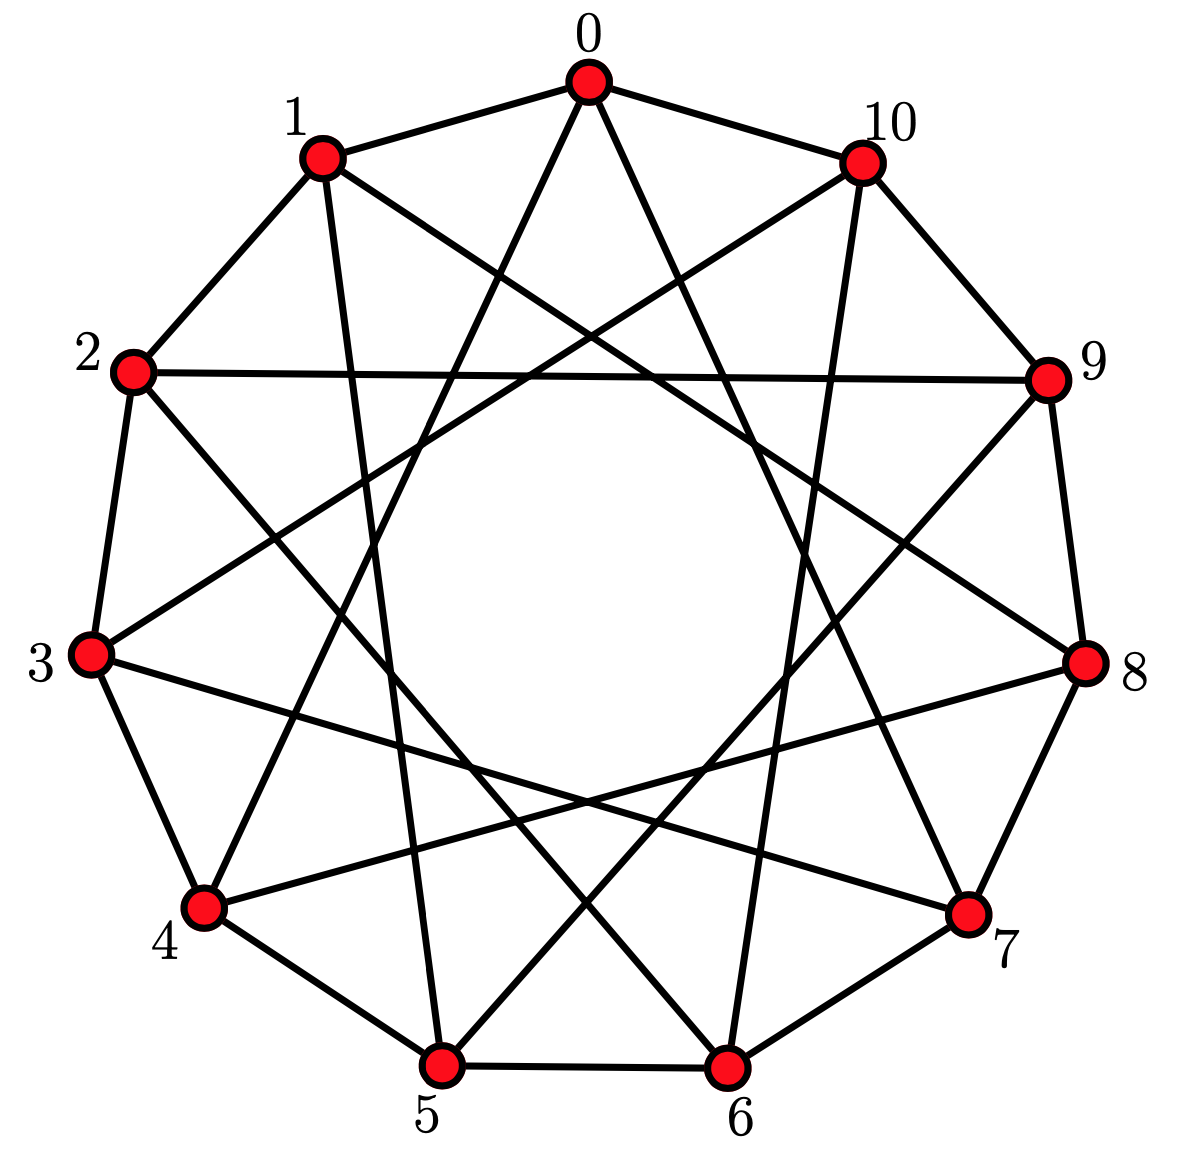
\includegraphics[width=8cm]{GRAPHICS/GRAPHS/cayley_mod11_1mod3}
$$
\caption{\label{fig:Cayley_Z11:1mod3}The Cayley graph in $\bbZ_{11}$}
\end{figure}
Let us draw the Cayley graph of $\Sym(5)$ with respect to the Coxter generators:
{\tt
\input GRAPHICS/THE_MAKEFILE/EXTRACTS/Cayley_Sym5_coxeter_draw.tex
}
The drawing is shown in Figure~\ref{fig:Cayley_Sym5:coxeter}.
\begin{figure}
$$
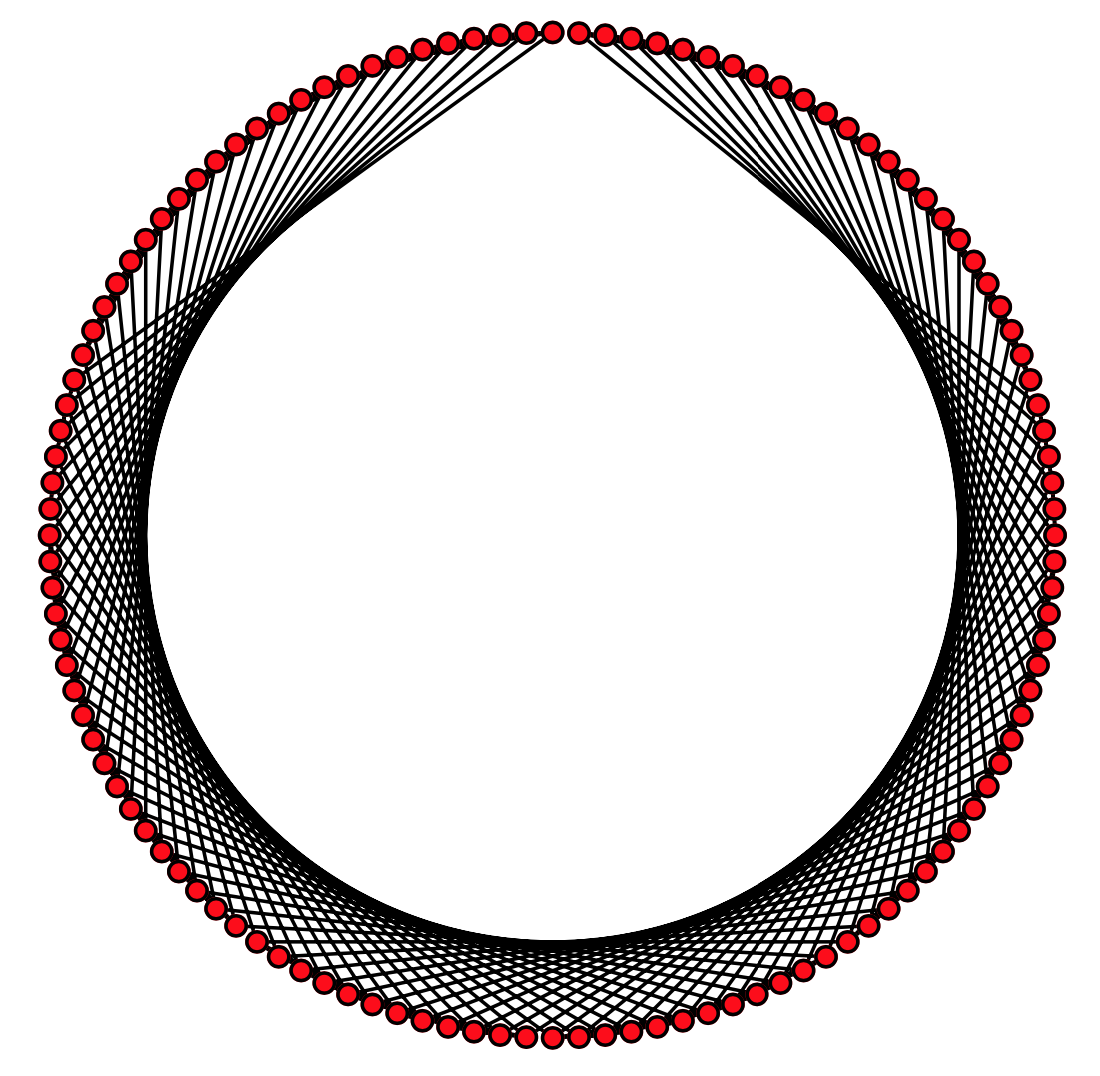
\includegraphics[width=9cm]{GRAPHICS/GRAPHS/sym5_coxeter}
$$
\caption{\label{fig:Cayley_Sym5:coxeter}The  Cayley graph of $\Sym(5)$ w.r.t. the Coxeter generators}
\end{figure}


\bigskip


It is possible to create the collinearity graph of an incidence structure. 
The incidence structure must be encoded by means of an incidence matrix. 
Let us continue an example from Section~\ref{sec:orthogonal}, 
where the incidence matrix of $Q(4,2)$ was created. 
At that time, we wrote the incidence matrix to file. 
Here, we read the incidence matrix from file and create the collinearity graph of it:
{\tt
\input GRAPHICS/THE_MAKEFILE/EXTRACTS/PGO_5_2_collinearity_graph.tex
}
The command also computes properties of the graph. 
The graph has 15 vertices of degree 6. 
This is because in the geometry, each point lies on three lines, 
and hence is collinar with 6 other points.




\bigskip



%Many more examples.




Table~\ref{tab:graphoptions} lists the Orbiter commands to classify graphs and tournaments. 
\begin{table}
\begin{center}
\begin{tabular}{|p{4cm}|c|p{7cm}|}
\hline
Command & Arguments & Purpose \\
\hline
\hline
\verb'-girth' & $d$ & Girth at least $d$ \\
\hline  
\verb'-regular' & $r$ & Regular of degree $r$ \\
\hline
\verb'-no_transmitter' & & Tournament without transmitter (requires \verb'-tournament') \\
\hline
\end{tabular}
\end{center}
\caption{\label{tab:graphoptions}Options for classifying graphs}
\end{table}
The following command classifies all graphs on 5 vertices:
{\tt
\input GRAPHICS/THE_MAKEFILE/EXTRACTS/graph_classify_5.tex
}
After the classification, the graphs with 5 edges are shown. 
The graph drawings are shown in Figure~\ref{fig:graph:drawings:v5}.
\begin{figure}
\input GRAPHICS/GRAPHS_5/graphs_v5_rep_5_0.tex
\input GRAPHICS/GRAPHS_5/graphs_v5_rep_5_1.tex
\input GRAPHICS/GRAPHS_5/graphs_v5_rep_5_2.tex
\input GRAPHICS/GRAPHS_5/graphs_v5_rep_5_3.tex
\input GRAPHICS/GRAPHS_5/graphs_v5_rep_5_4.tex
\input GRAPHICS/GRAPHS_5/graphs_v5_rep_5_5.tex
\caption{\label{fig:graph:drawings:v5}The graphs on 5 vertices with 5 edges}
\end{figure}


\bigskip


The next command classifies all tournaments on 4 vertices:
{\tt
\input GRAPHICS/THE_MAKEFILE/EXTRACTS/tournament_classify_4.tex
}
There are four tournaments. 
The graph drawings are shown in Figure~\ref{fig:graph:drawings:v5}.
\begin{figure}
\input GRAPHICS/TOURNAMENT_4/tournament_4_rep_6_0.tex
\input GRAPHICS/TOURNAMENT_4/tournament_4_rep_6_1.tex
\input GRAPHICS/TOURNAMENT_4/tournament_4_rep_6_2.tex
\input GRAPHICS/TOURNAMENT_4/tournament_4_rep_6_3.tex
\caption{\label{fig:graph:drawings:tournaments}The tournaments}
\end{figure}


%Figure~\ref{fig:t4} shows the resulting list of 4 tournaments.
%\begin{figure}
%$$
%
\includegraphics[width=11cm]{GRAPHICS/t4}
%$$
%\caption{\label{fig:t4}The four isomorphism types of tournaments on 4 vertices}
%\end{figure}

\bigskip

The next command classifies all cubic graphs on 8 vertices:
{\tt
\input GRAPHICS/THE_MAKEFILE/EXTRACTS/graph_classify_8_r3.tex
}
There are six cubic graphs. 
The graph drawings are shown in Figure~\ref{fig:graph:drawings:cubic:8}.
\begin{figure}
\input GRAPHICS/GRAPHS_CUBIC_8/graphs_v8_r3_rep_12_0.tex
\input GRAPHICS/GRAPHS_CUBIC_8/graphs_v8_r3_rep_12_1.tex
\input GRAPHICS/GRAPHS_CUBIC_8/graphs_v8_r3_rep_12_2.tex
\input GRAPHICS/GRAPHS_CUBIC_8/graphs_v8_r3_rep_12_3.tex
\input GRAPHICS/GRAPHS_CUBIC_8/graphs_v8_r3_rep_12_4.tex
\input GRAPHICS/GRAPHS_CUBIC_8/graphs_v8_r3_rep_12_5.tex
\caption{\label{fig:graph:drawings:cubic:8}The cubic graphs}
\end{figure}



A clique in a graph $\Gamma = (V,E)$ is a subset $S$ of the vertices 
such that any two elements of $S$ are adjacent in $\Gamma.$
Finding and classifying cliques in graphs is important for many applications of graph theory. 
Orbiter can help. 
The command \verb'-find_cliques' command from 
Table~\ref{tab:graphactivities} can be used to find all cliques in a graph.
Additional options for this command are shown in 
Table~\ref{tab:graphcliques}.
\begin{table}
\begin{center}
\begin{tabular}{|p{4cm}|c|p{7cm}|}
\hline
Command & Arguments & Purpose \\
\hline
\hline
\verb'-rainbow' &  & Find all rainbow cliques. The size of the cliques is the number of vertex colors. \\
\hline
\verb'-target_size' & $s$  & Find all cliques of size $s$. \\
\hline
\verb'-weighted' & $s$  & Find weighted cliques. \\
\hline
\verb'-Sajeeb' &   & Use the implementation by Sajeeb Chowdhury. \\
\hline
\verb'-output_file' &  fname & Write cliques to the named file. \\
\hline
\verb'-restrictions' &  $l$ $r$  $m$ & Restricted search: At level $l$, restrict to all branches congruent to $r$ modulo $m$. Here, $0 \le r < m.$ \\
\hline
\end{tabular}
\end{center}
\caption{\label{tab:graphcliques}Clique Finding Options}
\end{table}
For instance, the cliques of size 3 in the graph \verb'graph_v5_e7.colored_graph' from Section~\ref{sec:graphtheory} can be found using
{\tt
\input GRAPHICS/THE_MAKEFILE/EXTRACTS/small_graph_cliques.tex
}
This command finds three cliques of size 3.

\bigskip

It is also possible to classify all cliques under the automorphism group of the graph. 
This is a multi-step process, though. At first, the automorphism group of the graph has to be computed. 
Then, poset classification can be invoked to classify the cliques of a certain size. 
Here is an example.
We wish to classify the cliques in the Paley graph of order 13. 
The first command creates the graph and computes the automorphism group:
{\tt
\input GRAPHICS/THE_MAKEFILE/EXTRACTS/Paley_13_aut.tex
}
The command writes a file \verb'Paley_13_group.makefile', shown below: 
{\tt
\input GRAPHICS/THE_MAKEFILE/Paley_13_group_makefile.tex
}
The group is given using a base and strong generating set. 
The base 
consists of the two points $0,1.$ 
Three strong generators with respect to this base are given in a csv file.
Using this group, 
the next command classifies all cliques of size at most 5 in the Paley graph of order 13 
under the action of the automorphism group. 
It turns out that there are no 5-cliques, and that the largest cliques have size 3. 
The command shows that there is a unique orbit of 3-cliques:
{\tt
\input GRAPHICS/THE_MAKEFILE/EXTRACTS/Paley_13_cliques_classify.tex
}
For comparison, the command 
{\tt
\input GRAPHICS/THE_MAKEFILE/EXTRACTS/Paley_13_cliques_all.tex
}
finds all cliques of size 3. There are exactly 26 of them. 
Because of the previous command, we know that they are all equivalent under 
the automorphism group of the graph.


\bigskip

Let us consider the orbital graph created in Section~\ref{sec:graphtheory}.
We wish to study the 5-cliques. 
We first determine the number of 5-cliques, 
and then the number of orbits of 5-cliques under the automorphism group. 
The following command computes all 5-cliques:
{\tt
\input GRAPHICS/THE_MAKEFILE/EXTRACTS/HJ64_cliques5.tex
}
It turns out that there are exactly 1008 5-cliques.
Concerning the classification with respect to the automorphism group of the graph, 
we apply the following command:
{\tt
\input GRAPHICS/THE_MAKEFILE/EXTRACTS/HJ64_cliques5_classify.tex
}
This command shows that all of the 1008 $5$-cliques lie in one orbit under the group. 
The orbit representative picked by Orbiter is $\{0,8,31,110,283\}.$ 
These numbers refer to the vertices of the graph. They are zero-based.
The stabilizer of the clique has order 1200.


\bigskip


Let us look at the collinearity graph of $Q(4,2)$ one more time. The following command computes the 
cliques of size 3:
{\tt
\input GRAPHICS/THE_MAKEFILE/EXTRACTS/PGO_5_2_cliques.tex
}
There are 15 cliques of size 3. They correspond to the lines in the geometry.

\bigskip


\section{Combinatorial Objects}
\label{sec:combinatorial:objects}


\input C14/sec_1.tex
	

\bigskip


\clearpage

\section{Encoding Combinatorial Objects}
\label{sec:combinatorial:objects:files}


\input C14/sec_2.tex
	

\bigskip


\clearpage

Combinatorial objects are objects that are defined by means of a finite group action.  
The isomorphism problem for combinatorial objects is the question 
to decide whether two objects of the same type belong to 
the same orbit under the relevant group action. 
Orbiter offers a unified treatment of such questions for various types of objects.
The main tool is the computation of a canonical form, as well as the automorphism group. 

\bigskip

Combinatorial objects are coded as sequences of integers.
Each type of object has its own coding. 
Coding of objects as integer sequences allows easy handling of objcts. 
For instance, objects can be specified in a command line argument, or they can be stored in a file.
Large numbers of objects can be stored in files.

\bigskip

In order to apply Orbiter commands, an input stream is defined. 
An input stream is a sequence of objects, all of the same kind. 
The objects can be defined using any of the commands listed in Table~\ref{tab:combinatorial:objects}.
The file types will be discussed in more detail in the next section.
\begin{table}
	\begin{center}
	\begin{tabular}{|p{4cm}|p{3cm}|p{7cm}|}
		\hline
		Command & Arguments & Purpose \\
		\hline
		\hline
		\verb'-set_of_points' &  & A set consisting of points.  \\
		\hline
		\verb'-set_of_lines' &  & A set consisting of lines.  \\
		\hline
		\verb'-set_of_points_' \verb'and_lines' &  & A set consisting of points and a second set consisting of lines.  \\
		\hline
		\verb'-set_of_packing' &  &  A set of packings. \\
		\hline
		\verb'-file_of_points' &  &  A set consisting of points read from file. \\
		\hline
		\verb'-file_of_lines' &  &  A set consisting of lines read from file. \\
		\hline
		\verb'-file_of_packings' &  &   A set consisting of packings read from file. \\
		\hline
		\verb'-file_of_packings' \verb'_through_spread' \verb'_table' &  & A file of packings.  \\
		\hline
		\verb'-file_of_point_set' &  & A file containing point sets.  \\
		\hline
		\verb'-file_of_designs' &  &  A file containing designs or large sets. \\
		\hline
		\verb'-file_of_incidence' \verb'_geometries' & $v$ $b$ $f$ &  
		A file of incidence geometries defined by their set of flags. 
		Here, $v$ is the number of points, $b$ is the number of blocks and $f$ is the number of flags.\\
		\hline
		\verb'-file_of_incidence' \verb'_geometries_by' \verb'_row_ranks' &  &  A file describing incidence geometries defined by their row ranks. \\
		\hline
		\verb'-incidence_geometry' & flags $v$ $b$ $f$  & An incidence geometry defined by a set of flags. 
		Here, $v$ is the number of points, $b$ is the number of blocks and $f$ is the number of flags.\\
		\hline
		\verb'-incidence_geometry' \verb'_by_row_ranks' &  & An incidence geometry defined by row ranks. \\
		\hline
		\verb'-from_parallel_' \verb'search' &  &   \\
		\hline
		\end{tabular}
	\end{center}
	\caption{\label{tab:combinatorial:objects}Defining Combinatorial Objects}
\end{table}
Here are some examples. First, we create the Hirschfeld surface.
Since the Hirschfeld surface is a cubic surface, 
the object is defined using point ranks in the relevant projective space 
as described in Section~\ref{sec:indexing:points}. 
For instance, the Hirschfeld surface in $\PG(3,4)$ is defined as 45 points, 
coded as 45 integers which are point ranks.
A makefile variable is employed to define the set.
The makefile variable is then used to define a set-object:
{\tt
\input GRAPHICS/THE_MAKEFILE/EXTRACTS/HIRSCHFELD_SURFACE_Q4_SET_OF_POINTS.tex
}
{\tt
\input GRAPHICS/THE_MAKEFILE/EXTRACTS/Hirschfeld_q4_from_set.tex
}
The next example creates the two hyperovals in $\PG(2,16).$ 
The hyperovals are stored in makefile variables:
{\tt
\input GRAPHICS/THE_MAKEFILE/EXTRACTS/HYPEROVAL_16_144.tex
}
{\tt
\input GRAPHICS/THE_MAKEFILE/EXTRACTS/HYPEROVAL_16_16320.tex
}
{\tt
\input GRAPHICS/THE_MAKEFILE/EXTRACTS/hyperoval_16_create.tex
}
In the next example, we read the points 
of an elliptic curve from file (see Section~\ref{sec:indexing:points}):
{\tt
\input GRAPHICS/THE_MAKEFILE/EXTRACTS/EC_read.tex
}
In the next example, we read a packing, 
using a previously defined table of spreads, stored in a csv file.
{\tt
\input GRAPHICS/THE_MAKEFILE/EXTRACTS/PG_3_5_assume_31_read.tex
}
The following command reads a file of large sets of designs:
{\tt
\input GRAPHICS/THE_MAKEFILE/EXTRACTS/LS_AG_2_3_read.tex
}
The next command reads incidence geometries from a file containing the flags:
{\tt
\input GRAPHICS/THE_MAKEFILE/EXTRACTS/geo_7_3_read.tex
}
The next command creates incidence geometries from a file containing row-ranks:
{\tt
\input GRAPHICS/THE_MAKEFILE/EXTRACTS/Desargues_path_lex_least_read.tex
}

Combinatorial objects can be stored in text files. 
There can be any number of objects in one file.
The objects themselves are coded. 
For instance, a set of points in projective space 
is given as a set of integers, using the Orbiter point ranks. 
Likewise, a set of lines is coded using Orbiter line ranks. 
For designs, there are several ways in which the object can be stored. 
One way is by listing the incidences in a numerical form. 
One number is one incidence. 
Another way is by describing the incidence matrix in a row-by-row fashion, using ranks of $k$-subsets.
This assumes that the number of incidences per row is constant over all rows.  
Yet another way is by listing the columns of the incidence matrix, again using ranks of $k$-subsets. 
This version requires that the column sums of the incidence matrix are constant.
Let us go over some of these file formats, using small examples to illustrate the ideas informally.


\bigskip


Suppose we want to work with the Pasch configuration. 
This is the configuration of 6 points and 4 lines 
shown in Figure~\ref{fig:Pasch}.
\begin{figure}
$$
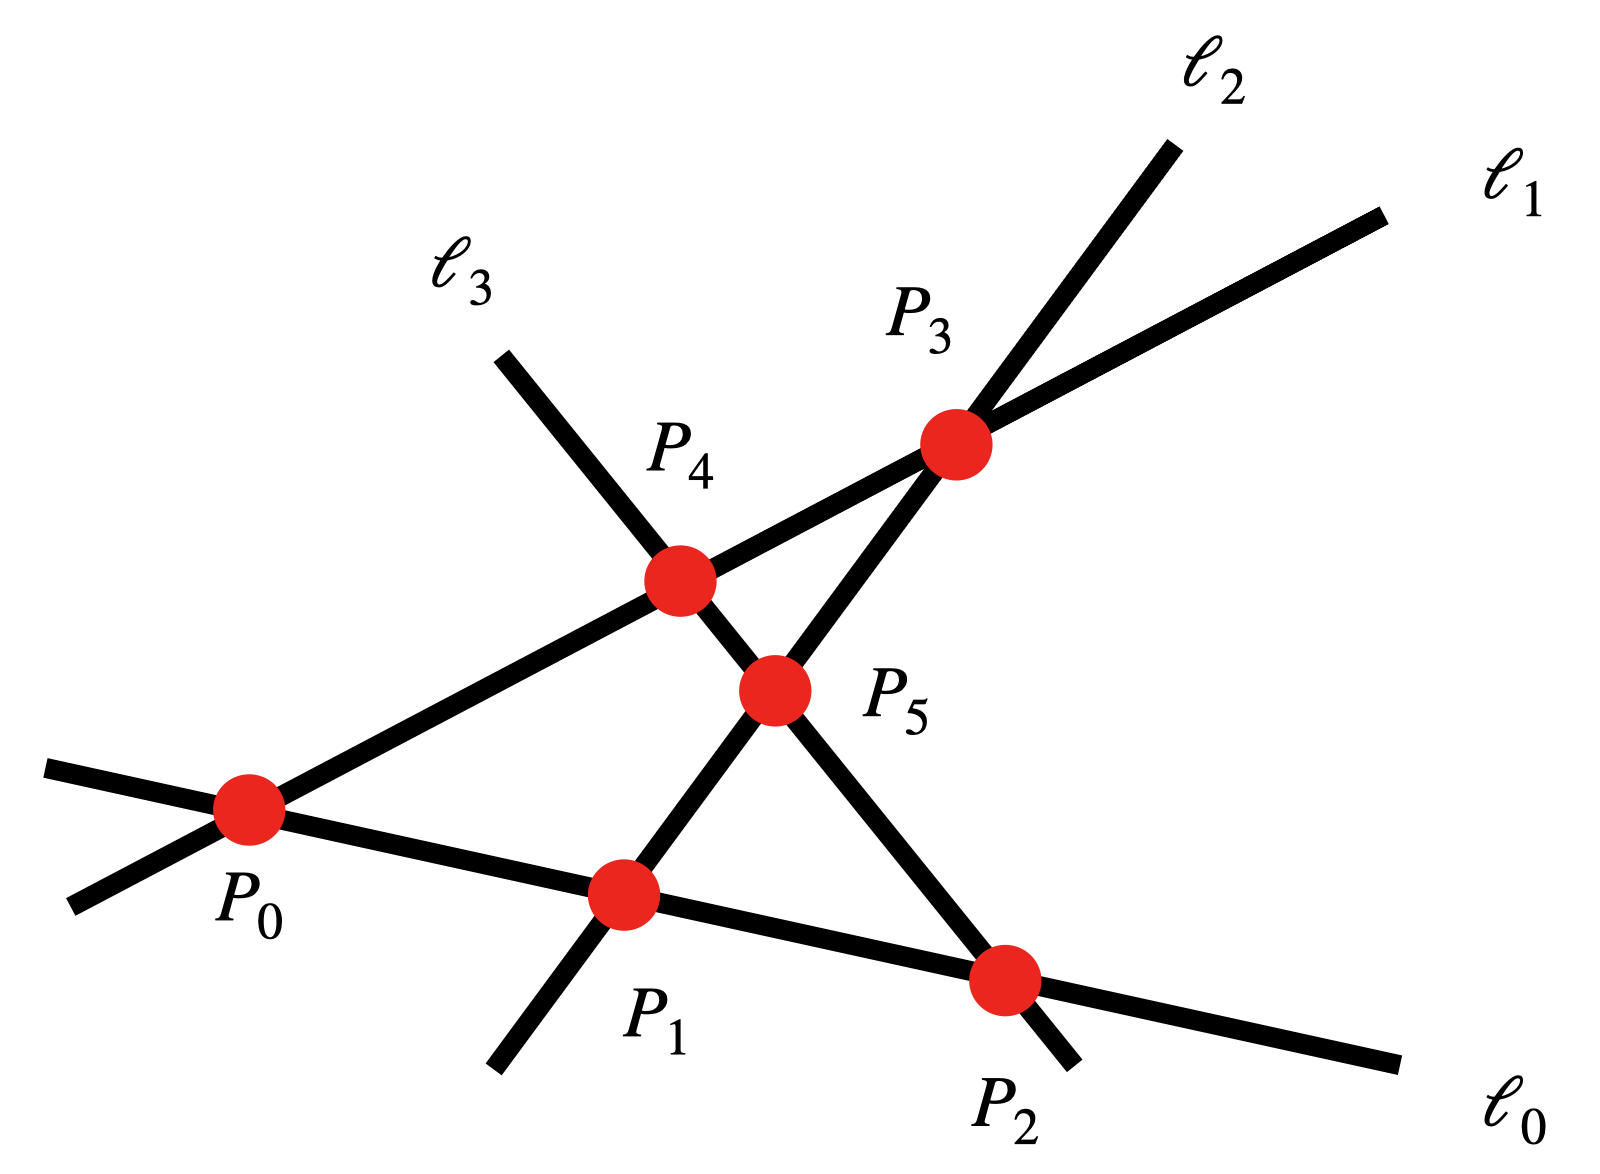
\includegraphics[width=10cm]{GRAPHICS/PASCH/pasch}
$$
\caption{\label{fig:Pasch}The Pasch configuration}
\end{figure}
In the geometry, we have 4 lines, which we can identify with the index sets of the points as
$\{0,1,2\},$ $\{0,3,4\},$ $\{1,3,5\}$ and $\{2,4,5\}.$ 
The incidence matrix of the configuration is shown in Figure~\ref{fig:Pasch:incma}.
Row labels are on the left, column labels are on top.
The $(i,j)$-entry is one if $P_i$ lies on $\ell_j,$ and it is zero otherwise.
\begin{figure}
$$
\begin{array}{c|cccc}
& \ell_0 & \ell_1 & \ell_2 & \ell_3 \\
\hline
P_0 & 1 & 1 & 0 & 0 \\
P_1 & 1 & 0 & 1 & 0 \\
P_2 & 1 & 0 & 0 & 1 \\
P_3 & 0 & 1 & 1 & 0 \\
P_4 & 0 & 1 & 0 & 1 \\
P_5 & 0 & 0 & 1 & 1 \\
\end{array}
$$
\caption{\label{fig:Pasch:incma}The incidence matrix of the Pasch configuration}
\end{figure}
There are three ways to encode the incidence structure. 
One way encodes the flags of the geometry.
This will be described next.
The flag space is the set of all possible flags in the incidence matrix between the given number of points and lines.
The space is totally ordered 
using the row-major ordering (see Figure~\ref{fig:Pasch:incma:row:major}).
\begin{figure}
$$
\begin{array}{c|cccc}
& \ell_0 & \ell_1 & \ell_2 & \ell_3 \\
\hline
P_0 & 0 & 1 & 2 & 3 \\
P_1 & 4 & 5 & 6 & 7 \\
P_2 & 8 & 9 & 10 & 11 \\
P_3 & 12 & 13 & 14 & 15 \\
P_4 & 16 & 17 & 18 & 19 \\
P_5 & 20 & 21 & 22 & 23 \\
\end{array}
$$
\caption{\label{fig:Pasch:incma:row:major}Row-major ordering of the flag space}
\end{figure}
The Pasch configuration can now be coded as 
$$
\{0,1,4,6,8,11,13,14,17,19,22,23\}.
$$
The file \verb'pasch.inc' contains:
\begin{verbatim}
6 4 12
0 1 4 6 8 11 13 14 17 19 22 23 
-1 1
24
\end{verbatim}
The first line lists the number of rows and columns of the incidence matrix, and the number of incidences. 
The geometry is encoded on the next line. After that, a marker of -1 shows that this is the only 
geometry in this file (the file format allows for any number of incidence geometries, all with the same parameters).
The final row is the order of the automorphism group of the geometry. 
This row is optional. In case that there are several geometries in the file, 
the orders will all be listed. In this case, the possible values will be 
collected with multiplicities, and listed in decreasing order.
The command 
{\tt
\input GRAPHICS/THE_MAKEFILE/EXTRACTS/geo_pasch_read.tex
}
reads the incidence geometry from the file \verb'pasch.inc'.
It is also possible to enter the incidence geometry directly from the command line. The following example 
uses the \verb'-incidence_geometry' command to do so:
{\tt
\input GRAPHICS/THE_MAKEFILE/EXTRACTS/geo_pasch_given.tex
}



\section{Overview of Canonical Forms}
\label{sec:canonical:form:overview}


\input C15/sec_1.tex
	

\bigskip


\clearpage




\section{Canonical Forms of Objects in Projective Space}
\label{sec:canonical:form:objects:PG}


\input C15/sec_2.tex
	

\bigskip


\clearpage

\section{Canonical Forms of Incidence Geometries}
\label{sec:canonical:form:objects:incidence:geometries}


\input C15/sec_3.tex


\bigskip


\clearpage


\section{Canonical Forms of Objects from Design Theory}
\label{sec:canonical:form:objects:design:theory}


\input C15/sec_4.tex


\bigskip


\clearpage


\section{Canonical Forms of Linear Codes}
\label{sec:canonical:form:objects:linear:codes}


\input C15/sec_5.tex


\bigskip


\clearpage

\section{Canonical Forms of General Codes}
\label{sec:canonical:form:objects:general:codes}


\input C15/sec_6.tex


\bigskip


\clearpage




\section{Canonical Forms of Graphs}
\label{sec:canonical:form:objects:graphs}


\input C15/sec_7.tex


\bigskip


\clearpage



\section{Canonical Forms of Quartic Curves}
\label{sec:canonical:form:objects:quartic:curvs}


\input C15/sec_8.tex


\bigskip


\clearpage




What is a combinatorial object? For the purposes of Orbiter, 
it is any kind of  object that has a representation as a set of sets, 
all drawn from an underlying finite set. 
We allow colorings of the elements of the underlying set and of the sets in the set-system.
The representation is functorial. 
Isomorphisms between the combinatorial objects 
must correspond to color preserving bijections of the set-representation and vice-versa.
Under these conditions, the isomorphisms  between  combinatorial objects and automorphisms from one object to itself 
correspond to the mappings between the associated set representations. 


\bigskip

The set-representation of combinatorial objects can help us computationally approach the isomorphism problem. 
We simply search for color-preserving bijections that take the set-representation of the object to 
the set-representation of the other object. Automorphisms can be found by mapping 
the set-representation of the object to itself.


\bigskip

Canonical labelings can be used to eliminate the need to do pairwise isomorphism testing. 
This is particularly helpful if the number of objects to test is large. 
If we have $N$ objects, say,  then pairwise isomorphism testing requires ${N\choose 2}$ tests. 
With canonical forms, we only need $N$ canonical forms computations.

\bigskip


Sets of sets are incidence structures.
The Levi graph of an incidence structure is the bipartite graph 
whose two classes correspond to rows and columns 
of the incidence matrix. The partition of the set system (underlying point set and set of sets) 
reduces to a coloring of the vertices of the graph.
Two combinatorial objects are isomorphic if and only if the associated colored 
Levi graphs are isomorphic in the sense of graph isomorphism. 
This allows to settle many questions associated with combinatorial object, such as 
isomorphism testing and determining the automorphism group.

\bigskip

A canonical labeling of a graph is a bijection of the vertices. 
The property is that if two graphs are isomorphic, then the 
graphs become identical if the canonical labeling permutation is applied 
(each graph has its own canonical labeling). 
It is therefore important to compute canonical forms.
If there is a vertex coloring, 
we implicitly assume that the canonical labeling preserves the coloring.

\bigskip

The graph theory package Nauty~\cite{Nauty2020} provides a canonical form algorithm for graphs. 
Using the Levi graph construction, this technique allows to solve the isomorphism problem for 
combinatorial objects in the more general sense just defined.

\bigskip


The technique of isomorphism testing can be lifted to combinatorial objects in projective spaces 
or other types of finite incidence geometries. 
For instance, arcs in projective planes have been 
classified this way (cf.~\cite{AlogaidiBetten}).

\bigskip


Table~\ref{tab:canonical} list Orbiter commands related 
to canonical labelings of combinatorial objects.
\begin{table}
\begin{center}
\begin{tabular}{|p{5cm}|p{2cm}|p{7cm}|}
\hline
Command & Arguments & Purpose \\
\hline 
\verb'-max_TDO_depth' & $d$  & Limit TDO depth to $d$ in the report.\\
\hline
\verb'-classification_prefix' & prefix  & Use the given prefix when writing files related to the classification.\\
\hline
\verb'-save_ago' &   & Save the automorphism group orders to file.\\
\hline
\verb'-save_transversal' &   & Save the indices of the elements chosen for the transversal.\\
\hline
\end{tabular}
\end{center}
\caption{\label{tab:canonical}Orbiter commands related to canonical labelings}
\end{table}

\bigskip




Suppose we want to compute the stabilizer of an elliptic curve.
In Section~\ref{sec:FPG}, we have created an elliptic curve over $\bbF_{11}$ 
and stored the set of $\bbF_q$-points in the file 
$$
\verb'elliptic_curve_b1_c3_q11.txt'.
$$
The following example computes the set stabilizer of the curve.
This means it computes the set stabilizer of the points on the curve. 
In order to do so, an input stream is created which referst to the file 
containing the Orbiter point ranks of points on the curve. 
{\tt
\input GRAPHICS/THE_MAKEFILE/EXTRACTS/EC_canon.tex
}
Orbiter shows that the curve has a collineation stabilizer of order 6, 
generated by 
\begin{mdframed}[style=MyFrame]
\input GRAPHICS/LATEX/nauty_stab_EC.tex
\end{mdframed}

\bigskip

The following example computes the canonical form 
and the automorphism group of the Hirschfeld surface in $\PG(3,4)$. 
Using indexing of points in $\PG(3,4)$, we encode the 
surface as a set of points using Orbiter ranks.
We use a makefile variable to provide these ranks as input for the canonical form procedure.
{\tt
\input GRAPHICS/THE_MAKEFILE/EXTRACTS/HIRSCHFELD_SURFACE_Q4_SET_OF_POINTS.tex
}
{\tt
\input GRAPHICS/THE_MAKEFILE/EXTRACTS/Hirschfeld_q4_c.tex
}
{\tt
\input GRAPHICS/THE_MAKEFILE/EXTRACTS/Hirschfeld_q4_set_c.tex
}

\bigskip

In the next example, we compute the canonical form of the two hyperovals in $\PG(2,16).$
{\tt
\input GRAPHICS/THE_MAKEFILE/EXTRACTS/hyperoval_16_canonical_form.tex
}

\bigskip

In the next example, we compute the set stabilizers of orbits of $\PGL(4,2)$ on subsets of $\PG(3,2),$ 
as computed earlier in Section~\ref{sec:subsetorbits}, using the command \verb'PG_3_2_subsets'.
These orbits are relevant for Section~\ref{sec:cubicsurfaces:Dickson}. 
Concerning the work in Dickson~\cite{Dickson15} only subsets whose size is odd are relevant, 
so we restrict to those subsets:
{\tt
\input GRAPHICS/THE_MAKEFILE/EXTRACTS/Dickson_sets_stabilizer.tex
}

\bigskip

There are two ovoids in $\PG(3,2).$ The classical ovoid is the elliptic quadric. It was created using the command \verb'elliptic_quadric_ovoid_q8' in Section~\ref{sec:geometric:objects}.
The following command computes the stabilizer of the ovoid:
{\tt
\input GRAPHICS/THE_MAKEFILE/EXTRACTS/ovoid_q8_canon.tex
}
The other ovoid is the Suzuki Tits ovoid,  which was created using the command \verb'ovoid_ST_q8' in Section~\ref{sec:geometric:objects}.
The stabilizer of the Suzuki Tits ovoid is the Suzuki group.
The following command computes this group for $q=8.$
{\tt
\input GRAPHICS/THE_MAKEFILE/EXTRACTS/ovoid_ST_q8_canon.tex
}
We can store the generators in a makefile variable as follows:
{\tt
\input GRAPHICS/THE_MAKEFILE/EXTRACTS/SUZUKI_8_GENERATORS.tex
}
We can now recover the Suzuki group using the command:
{\tt
\input GRAPHICS/THE_MAKEFILE/EXTRACTS/Suzuki_8.tex
}


\bigskip


Let us consider system of subsets. 
This subsets are chosen from the same set, which we call the underlying set. 
The elements of the group set are often called points.
In many cases, there are conditions that restrict the way in which the sets can be chosen. 
There is a notion of isomorphism on such set systems. 
Two set systems are isomorphic is there is a bijection between the underlying 
sets which takes one to the other. 
The incidence matrix is the 0/1 matrix whose rows correspond to the elements of the group set, 
and whose columns correspond to the chosen subsets. An entry 1 indicates that the 
corresponding point belongs to the corresponding set.

\bigskip


An incidence geometry is a set system with the following properties:
No set appears twice, and no pair of elements in the set appear in two different sets. 
The elements of the set are called points. 
The sets are called lines (or sometimes planes). 
A flag is an incident point-line pair.
An anti-flag is a non-incident point-line pair.
Two points are said to be collinear of there is a line in the geometry containing both points.

\bigskip


It is interesting to study the action of the automorphism group on the elements of a gemetry. 
Properties of interest are various levels of transitivity on the elements of the geometry. 
For instance, a geometry is line-transitive if the automorphism group is transitive on lines. 
Likewise, it is flag transitive if the automorphism group is transitive on flags.
The collinearity graph of a geometry is the graph whose vertices correspond to the points, 
with two vertices adjacent of the associated points are collinear.
The girth of the incidence geometry is the girth of the associated collineation graph. 
A geometry is triangle free if its girth is at least 4.



\bigskip


A configuration $v_r b_k$ is an incidence geometry 
on a set of size $v$ and with $b$ lines such that 
each line has size $k$ and each point is contained in exactly $r$ lines.
In the special case where $b=v$ and $k=r$, the name symmetric configuration $v_r$ is used 
(the term symmetric is somewhat misleading because the 
incidence matrix of a symmetric configuration need not be symmetric). 
Orbiter can be used to classify incidence geometries. 
One of the important steps in this process is computing a canonical form of the incidence gometry. 

\bigskip

We will also be producing drawings of the incidence matrices of geometries.
In these drawings, flags are indicated as heavy squares while 
anti-flags are drawn as small squares. 
The coloring will indicate the orbits of the automorphism group on flags and anti-flags. 
Objects with the same color belong to the same orbit. For a flag-transitive geometry, 
there is only one color for the incidences. 


\bigskip

The following command computes the canonical form  and a report 
of the projective plane $\PG(2,2)$, which is a configuration $7_3.$
{\tt
\input GRAPHICS/THE_MAKEFILE/EXTRACTS/geo_7_3_c.tex
}
A bitmap drawing is produced, as shown in Figure~\ref{fig:PG:2:2}.
\begin{figure}
$$
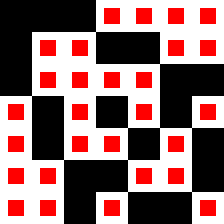
\includegraphics[width=6cm]{GRAPHICS/CONF/7_3_object0_INP_flag_orbits_draw}
$$
\caption{\label{fig:PG:2:2}Incidence matrix of the projective plane $\PG(2,2)$}
\end{figure}
The command also produces the following report of the geometry:
\begin{mdframed}[style=MyFrame]
\input GRAPHICS/LATEX/canon_7_3.tex
\end{mdframed}

\bigskip



The following command computes the canonical form  and a report 
of the affine plane $\AG(2,3)$, which is a configuration $9_4 12_3.$
{\tt
\input GRAPHICS/THE_MAKEFILE/EXTRACTS/AG_2_3_c.tex
}
A bitmap drawing is produced, shown in Figure~\ref{fig:AG:2:3}.
\begin{figure}
$$
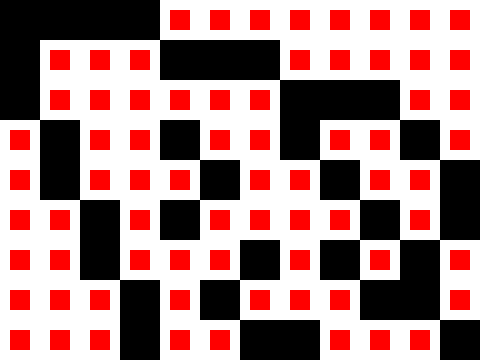
\includegraphics[width=8cm]{GRAPHICS/CONF/AG_2_3_object0_INP_flag_orbits_draw}
$$
\caption{\label{fig:AG:2:3}The affine plane $\AG(2,3)$ is a configuration $9_4 12_3$}
\end{figure}
Because the geometry is flag transitive, there is only one color being used for the incidence. 
In fact, all incidences are in black.
The geometry is also anti-flag transitive. This can be seen from the fact that there is 
only one color in the picture for the smaller boxes, which represent anti-flags.
Orbiter also produces the following report of the geometry:
\begin{mdframed}[style=MyFrame]
\input GRAPHICS/LATEX/canon_AG_2_3.tex
\end{mdframed}

\bigskip



It is possible to perform isomorph classification for configurations based on incidence files. 
Suppose we want to check that the configurations in \verb'10_3' are infact all nonisomorphic. We apply the 
canonical form algorithm given by Nauty.
This produces a transversal of the isomorphism types of incidence geometries from the given list of input objects.
The objects are specified by means of the \verb'combinatorial_objects' command. 
The classification algorithm can print a report which lists the transversal and all elements in it in latex form. 
{\tt
\input GRAPHICS/THE_MAKEFILE/EXTRACTS/geo_10_3_c.tex
}
The report is shown below. It is truncated for reasons of space.
Only the first two geometries are shown. 
Note that the ordering of geometries in the report may be different from the ordering in the input file. 
This is because the classification program sorts the geometries according to the canonical form.
Also, note that the report includes the incidence geometry in the form 
it is given as well as the tactical decomposition 
induced by the orbits of the automorphism group.
\begin{mdframed}[style=MyFrame]
\input GRAPHICS/10_3/10_3_report_truncated.tex
\end{mdframed}



\bigskip







The following command computes 
the canonical form for the three triangle free configurations $24_3$ found by Abdullah Alazemi. 
These configurations have $24$ points,
$24$ lines, each line consists of $3$ points and each point is on $3$ lines. 
{\tt
\input GRAPHICS/THE_MAKEFILE/EXTRACTS/FILE_24_3_TFC_INC.tex
}
{\tt
\input GRAPHICS/THE_MAKEFILE/EXTRACTS/TFC_24_3_c.tex
}
The command also computes the tactical decomposition induced by the automorphism group. 
In addition, the command also computes the orbits on flags and on anti-flags. 
The third of the three geometries is flag transitive.
A bitmap drawing is produced, shown in Figure~\ref{fig:flag:transitive:24}.
Because the geometry is flag transitive, there is only one color being used for the incidence. 
In fact, all incidences are in black.
\begin{figure}
$$
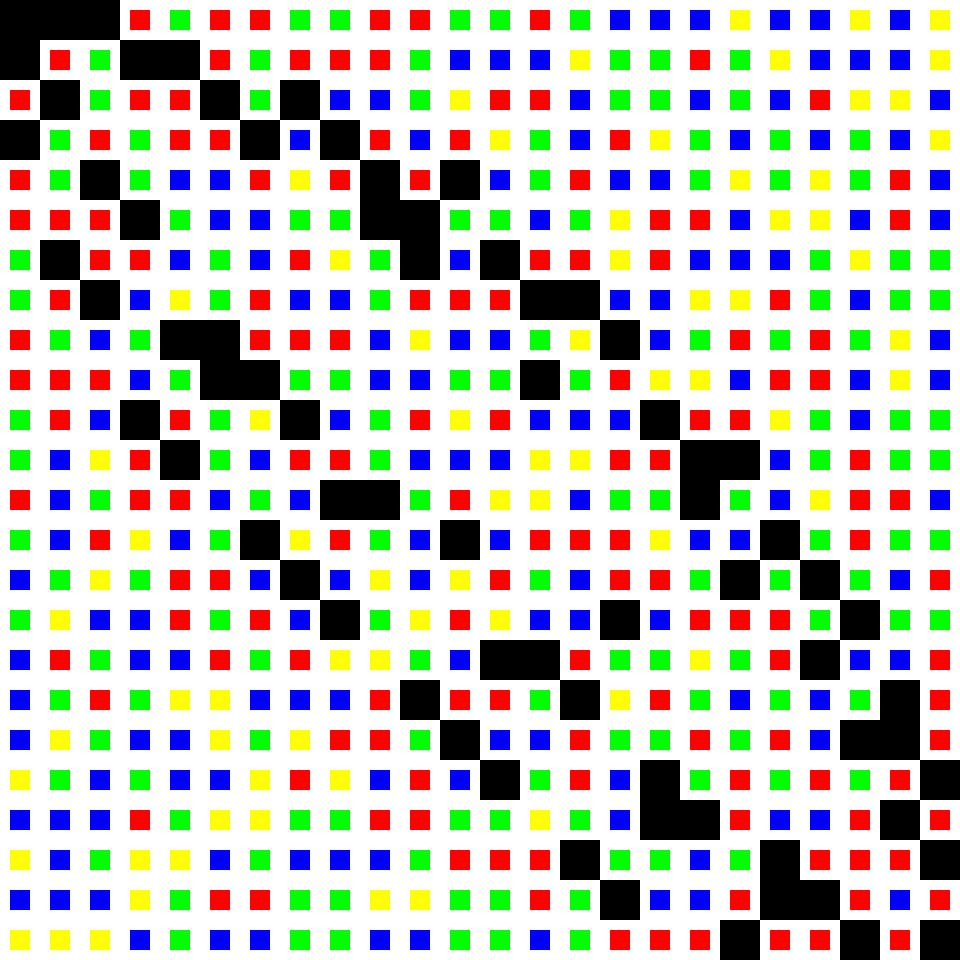
\includegraphics[width=8cm]{GRAPHICS/CONF/24_3_TFC_object2_TDA_flag_orbits_draw}
$$
\caption{\label{fig:flag:transitive:24}A flag transitive $24_3$ configuration}
\end{figure}
In Section~\ref{sec:design}, designs have been created. 
In order to compute properties of the design, we export the incidence matrix to file. 
After that, we compute the canonical form of the design, which allows us to determine many properties.
The following example computes the properties of $\PG(2,3)$:
{\tt
\input GRAPHICS/THE_MAKEFILE/EXTRACTS/design_PG_2_3_canonical.tex
}



\bigskip


The command 
{\tt
\input GRAPHICS/THE_MAKEFILE/EXTRACTS/wreath_product_designs_n4_k2_c.tex
}
computes the automorphism group of the design on 8 points created in Section~\ref{sec:design}.
The group is $\Sym(4) \wr \Sym(2)$.
The command 
{\tt
\input GRAPHICS/THE_MAKEFILE/EXTRACTS/wreath_product_designs_n8_k6_c.tex
}
computes the automorphism group of the design on 16 points created in Section~\ref{sec:design}.
The group is $\Sym(8) \wr \Sym(2)$.


\bigskip



In Section~\ref{sec:large:sets}, some large sets of $\AG(2,3)$ were constructed. 
The final isomorphism classifcation is performed using the Nauty interface. 
A list of combinatorial objects is created, and the  \verb'-canonical_form' command is applied as activity.
This will produce a list of pairwise non-isomorphic designs.
The size of this list is the number of isomorphism types of large sets of $\AG(2,3).$
{\tt
\input GRAPHICS/THE_MAKEFILE/EXTRACTS/LS_AG_2_3_solutions_classify.tex
}
It turns out that there are exactly two isomorphism types, 
with automorphism groups of order 54 and 42, respectively.

\bigskip

Orbiter can compute canonical forms and automorphism groups of codes using Nauty.
For linear codes, the semilinear automorphism group can be computed.

\bigskip


Consider the $[3,2,2]$ code generated by 
$$
\left[
\begin{array}{ccc}
	1&0&1\\
	0&1&1\\
\end{array}
\right]
$$
The semilinear automorphism group can be computed using the following command:
{\tt
\input GRAPHICS/THE_MAKEFILE/EXTRACTS/code_3_2_aut.tex
}
The code has a semilinear automorphism group of order 6.
The following report is written:
\begin{mdframed}[style=MyFrame]
\input GRAPHICS/LATEX/summary_of_orbits_code_3_2.tex
\end{mdframed}

\bigskip




The command 
{\tt
\input GRAPHICS/THE_MAKEFILE/EXTRACTS/CODE_RM_3_1_GENMA.tex
}
{\tt
\input GRAPHICS/THE_MAKEFILE/EXTRACTS/RM_3_1_group.tex
}
computes the automorphism group of the Reed-Muller code, of order 1344. 
It is the affine group $\AGL(3,2).$
A report is created, showing the automorphism group and the action on $\PG(3,2),$ with the Reed-Muller code distinguished.


\bigskip

The following command creates a drawing of the incidence matrix between points 
and lines in $\PG(3,2),$ 
with the Reed-Muller code distinguished:
%{\tt
%\input GRAPHICS/THE_MAKEFILE/EXTRACTS/REED_MULLER_3_1_CODEWORDS.tex
%}
{\tt
\input GRAPHICS/THE_MAKEFILE/EXTRACTS/RM_3_1_group_and_diagram.tex
}
The drawing in Figure~\ref{fig:RM:3:1:draw} is created.
\begin{figure}
$$
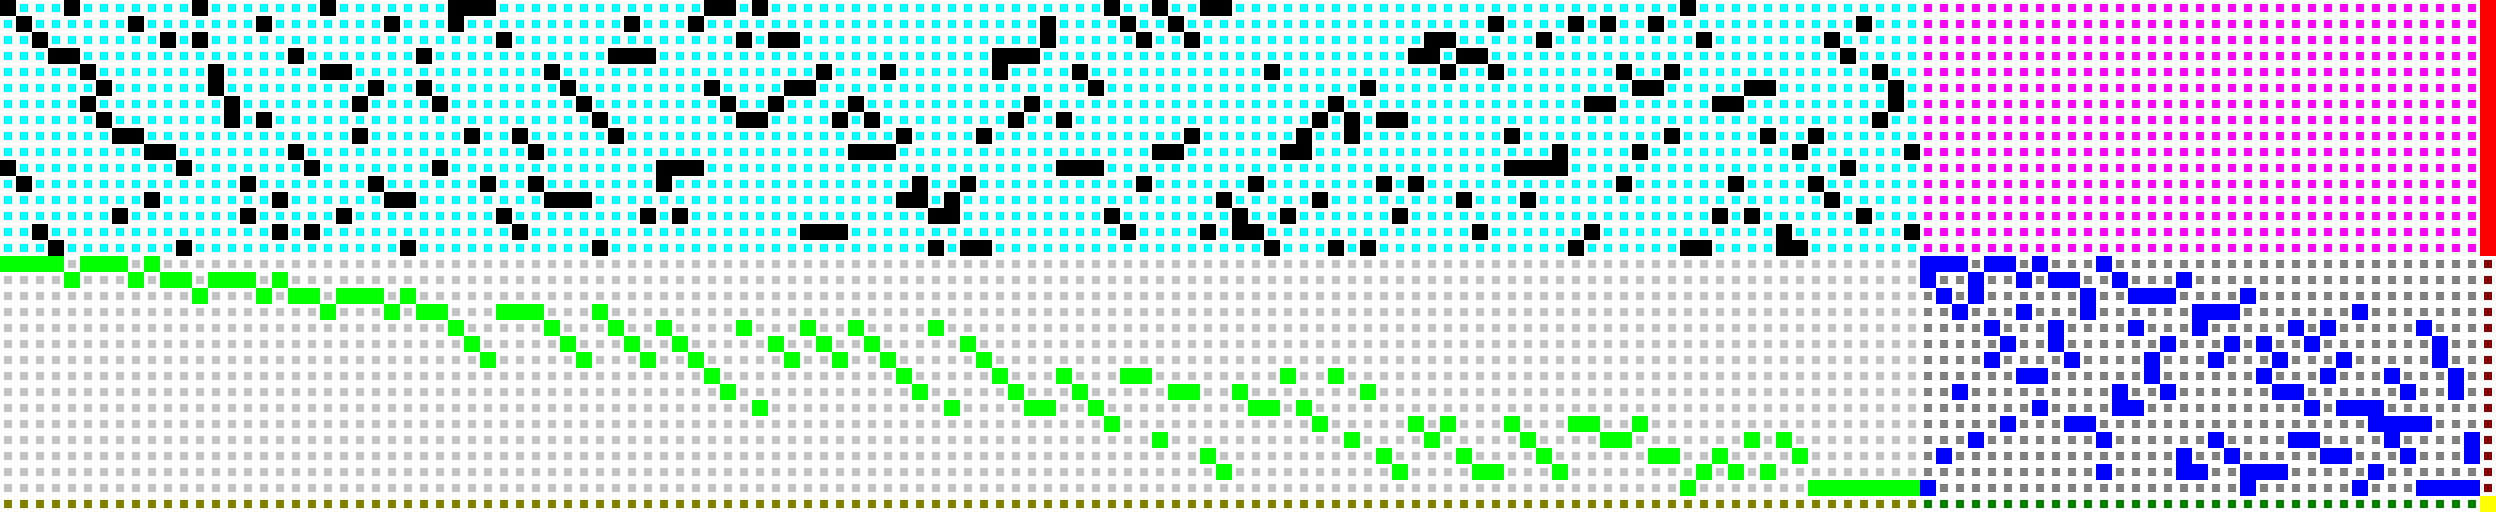
\includegraphics[width=15cm]{GRAPHICS/SEC_CODES/RM_4_1_object0_TDA_flag_orbits_draw}
$$
\caption{\label{fig:RM:3:1:draw}$\PG(3,2)$ with the Reed-Muller code distinguished}
\end{figure}


\bigskip




The command 
{\tt
\input GRAPHICS/THE_MAKEFILE/EXTRACTS/RS_6_4_7_group.tex
}
shows that the automorphism group has order $12$.
After some shortening, the output is:
\begin{mdframed}[style=MyFrame]
\input GRAPHICS/LATEX/RS_6_4_7.tex
\end{mdframed}

\bigskip


The command 
{\tt
\input GRAPHICS/THE_MAKEFILE/EXTRACTS/GV_n15_k6_d5_group.tex
}
computes the automorphism group of the Gilbert-Varshamov code from Section~\ref{sec:Bounds}. 
It has order $12$.

\bigskip

The command
{\tt
\input GRAPHICS/THE_MAKEFILE/EXTRACTS/HAMMING_CODE_CODEWORDS.tex
}
{\tt
\input GRAPHICS/THE_MAKEFILE/EXTRACTS/Hamming_graph_7_with_Hamming_code.tex
}
computes the set stabilizer of the Hamming code inside the automorphism group of the Hamming graph. 
The group has order $2688 = 16 \cdot 168$.

\bigskip
Orbiter can compute isomorphism and automorphism between graphs. 
Here are some examples.


\bigskip


Suppose we want to compute the automorphism group of the cycle graph of order 13:
{\tt
\input GRAPHICS/THE_MAKEFILE/EXTRACTS/Cycle_13_aut.tex
}
The output is two files: The first one, \verb'Cycle_13_group.makefile' is a makefile containing an Orbiter command to 
create the automorphism group:
The second file is \verb'Cycle_13_gens.csv', which contains the permutation representation of the group, and which is needed 
for the makefile.


\bigskip


The next command computes the automorphism group of the chain graph with respect to the partition $(2,3,2)$.
{\tt
\input GRAPHICS/THE_MAKEFILE/EXTRACTS/Chain_232_aut.tex
}
The following report is written:
\begin{mdframed}[style=MyFrame]
\input GRAPHICS/LATEX/chain_graph_aut.tex
\end{mdframed}




\bigskip

Junttila and Kaski maintain a collection of graphs that can be used as test cases.
The graphs are stored in Dimacs format and can be read in through 
the Orbiter \verb'-load_dimacs' command. 
For instance, the following command 
computes the automorphism group of the 
Levi graph of the desarguesian projective plane of order 16:
{\tt
\input GRAPHICS/THE_MAKEFILE/EXTRACTS/JK_graph_pp16_1.tex
}
The command shows a group of order 34217164800. 
As a measurement of the complexity, 
the number of backtrack nodes in Nauty is recorded:
\begin{verbatim}
nb_backtrack1 = 6
nb_backtrack2 = 134
nb_backtrack3 = 134
nb_backtrack4 = 1
\end{verbatim}
Here, 
\verb'nb_backtrack1' is the number of calls to \verb'firstpathnode', 
\verb'nb_backtrack2' is the number of calls to \verb'othernode', 
\verb'nb_backtrack3' is the number of calls to \verb'processnode', 
\verb'nb_backtrack4' is the number of calls to \verb'firstterminal'.
These are the four recursive functions in Nauty.

\bigskip

Unfortunately, the complexity of graph isomorphism is not well-understood. 
We can see this here.
While the first projective plane of order 16 can be handled relatively easily, 
the second one causes problems. The following command hardly finishes:
{\tt
\input GRAPHICS/THE_MAKEFILE/EXTRACTS/JK_graph_pp16_2.tex
}
The difference between the two planes is that the first plane 
has a very large automorphism group, while the second one has not. 
For any $q$, the Desarguesian plane $\PG(2,q)$ 
has the largest automorphism group 
of all projective planes of order $q$.




\bigskip


The following example considers the block intersection graph of 
a Steiner triple system (``STS'') of order 13. 
There are exactly two STS$(13)$. The one we consider here has a group of order 39. 
The block intersection graph has the same automorphism group.
{\tt
\input GRAPHICS/THE_MAKEFILE/EXTRACTS/JK_graph_sts_13.tex
}
The automorphism group has order 39 and is generated by:
\begin{verbatim}
(
(1, 25, 16)(2, 18, 20)(3, 7, 15)(4, 13, 11)(5, 6, 17)
(9, 12, 19)(10, 14, 24)(21, 23, 22), 
(0, 1, 2)(3, 4, 5)(7, 8, 9)(11, 12, 13)(14, 16, 18)
(15, 17, 19)(20, 22, 24)(21, 23, 25))
\end{verbatim}



\bigskip



Graphs can be created from groups by means of orbitals. An orbital is an orbit of a permutation 
group $G$ on the set of pairs. 
Here is an example. We start from the Coxeter-Tits graph on 315 vertices, whose automorphism group 
is the Hall-Janko group $J_2:2.$ 
We first read the graph from file \verb'halljanko315.csv' 
and compute the automorphism group using Nauty:
{\tt
\input GRAPHICS/THE_MAKEFILE/EXTRACTS/HJ_aut.tex
}
The next step is to compute the orbits of the automorphism group on pairs, using the following command:
{\tt
\input GRAPHICS/THE_MAKEFILE/EXTRACTS/HJ_group_and_orbits.tex
}
There are 4 orbits on pairs. 
We decide to pick the fourth orbit to create a new graph. Because indexing is zero-based, 
we give the orbit index of 3:
{\tt
\input GRAPHICS/THE_MAKEFILE/EXTRACTS/HJ_orbital_graph_3.tex
}
The graph is regular of degree 64. 

\bigskip

The next command computes the automorphism group of the collinearity graph of the $Q(4,2)$ quadric.
{\tt
\input GRAPHICS/THE_MAKEFILE/EXTRACTS/PGO_5_2_graph_group.tex
}
The group is $\PGO(5,2)$ of order 720. 
The command creates the group as a permutation group on the 15 vertices of the graph. 
The group is no longer treated as a matrix group. 

 
We wish to study the automorphism groups of certain quartic curves introduced by Edge.
We start by creating a cheat sheet of the field $\bbF_{17}$
{\tt
\input GRAPHICS/THE_MAKEFILE/EXTRACTS/F_17_edge.tex
}
Next, we compute the canonical form of the Edge quartic. 
This command also computes generators for the automorphism group of the curve.
{\tt
\input GRAPHICS/THE_MAKEFILE/EXTRACTS/Edge_curve_17_nauty.tex
}
Using the generators that have just been computed, 
we can recreate the group of the quartic curve:
{\tt
\input GRAPHICS/THE_MAKEFILE/EXTRACTS/Edge_curve_17_group.tex
}


\section{Graphical Output}
\label{sec:draw}


\input C16/sec_1.tex



\bigskip

\clearpage





\section{The Povray Interface}
\label{sec:povray}



\input C16/sec_2.tex



\bigskip
\clearpage




\section{Creating Animations}
\label{sec:animations}


\input C16/sec_3.tex



\bigskip

\clearpage






\section{Continuous Function Plotter}
\label{sec:function:plotter}


\input C16/sec_4.tex



\bigskip

\clearpage


Orbiter can produce graphical output in a variety of formats:
\begin{enumerate}
\item
TikZ / Latex~\cite{tantau:2022},
\item
Metapost~\cite{metapost2010},
\item
Bitmap files (.bmp)~\cite{bitmap},
\item
Povray, see Section~\ref{sec:povray}.
\end{enumerate}


\bigskip


Bitmaps can be created using the \verb'-draw_matrix' command. 
The input is an integer-valued matrix in csv format.
The matrix entries are translated into colors.
The possible commands after \verb'-draw_matrix' are shown in Table~\ref{tab:bitmap}.
\begin{table}
	\begin{center}
	\begin{tabular}{|p{4cm}|p{3cm}|p{7cm}|}
		\hline
		Command & Arguments & Purpose \\
		\hline
		\hline
		\verb'-input_csv_file' & csv-file  & Specify the inputcsv- file \\
		\hline
		\verb'-partition' & $w$ $R$ $C$  & Specify a partition $R$ of rows and $C$ of columns. Use separating lines of with $w$. \\
		\hline
		\verb'-box_width' & $w$  & Use $w$ pixels per matrix entry. \\
		\hline
		\verb'-bit_depth' & $d$  & Use  color bit depth of $d$ bits ($d=8$ or $d=24$). \\
		\hline
		\verb'-invert_colors' &   & Use an inverted color scheme. \\
		\hline
		\end{tabular}
	\end{center}
	\caption{\label{tab:bitmap}Commands to Create Bitmap Graphics}
\end{table}
Suppose we want to create a graphical representation of the addition table of the finite field $\bbF_7$.
The following command sequence first creates the addition and multiplication tables of the field, 
and then produces a bitmap graphic for the addition table:
{\tt
\input GRAPHICS/THE_MAKEFILE/EXTRACTS/F_7_tables.tex
}
The finite field activity  \verb'-cheat_sheet_GF' creates the file 
$$
\verb'GF_q7_addition_table.csv'
$$
which is used as the input for the second command. The file content is:
\begin{mdframed}[style=MyFrame]
\input GRAPHICS/LATEX/bitmap_output_csv_file.tex
\end{mdframed}
The second command 
creates the diagram in Figure~\ref{fig:F7}.
\begin{figure}
$$
\begin{array}{c}
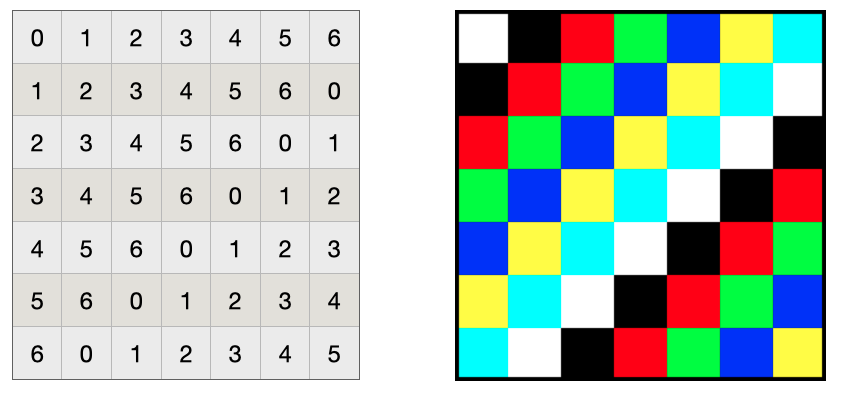
\includegraphics[width=13cm]{GRAPHICS/GF/F7_addition_table}\\
\end{array}
$$
\caption{\label{fig:F7}Addition table of $\bbF_7$}
\end{figure}
The \verb'-partition' command is used to define an outline of width 3 pixes. 
The all-in-one partition 7 is used as both row-partition and column-partition. 

\bigskip


The planes $\PG(2,q)$ admit a cyclic automorphism group known as the Singer cycle. 
The command 
{\tt
\input GRAPHICS/THE_MAKEFILE/EXTRACTS/PG_2_4_cyclic_incma.tex
}
produces a cyclically ordered incidence matrix of the plane $\PG(2,4),$ shown in 
Figure~\ref{fig:PG24:incma:transitive}.
\begin{figure}
$$
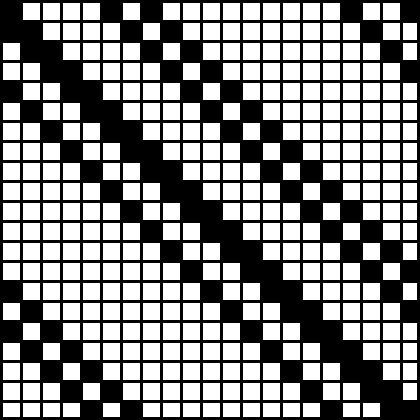
\includegraphics[width=7cm]{GRAPHICS/PG/PG_2_4_singer_incma_transitive_draw}
$$
\caption{\label{fig:PG24:incma:transitive}A cyclic ordering of the incidence matrix of $\PG(2,4)$}
\end{figure}
The 
Singer cycle is the projectivity defined by the companion matrix of an irreducible polynomial. 
We may pick the irreducible polynomial $X^2+X+\omega$ over $\bbF_4.$ 
The associated Singer cycle is the projectivity defined by the companion matrix 
$$
\left[
\begin{array}{ccc}
0&1&0\\
0&0&1\\
2&1&1\\
\end{array}
\right].
$$

\bigskip


The poset classification algorithm from Sections~\ref{sec:subsetorbits} 
and~\ref{sec:subspaceorbits} computes partially ordered sets. 
The posets are created using the \verb'-draw_poset' option in 
the poset classification control command package, see Table~\ref{tab:pc:options}. 
The posets are stored in a file with extension \verb'.layered_graph'.
These files can be drawn using the \verb'-draw_layered_graph' command.
The commands in Table~\ref{tab:draw:options} and Table~\ref{tab:draw:options:b} 
show ways in which to customize the drawings.
\begin{table}
\begin{center}
	\begin{tabular}{|p{4cm}|p{3cm}|p{7cm}|}
\hline
Command & Arguments & Purpose \\
\hline
\verb'-file' &  fname  & Use the given file name for output files. \\
\hline
\verb'-xin' &  $a$  & Assume input $x$-coordinates are in the interval $[0,a]$. Default value: 10000. \\
\hline
\verb'-yin' &  $a$  & Assume input $y$-coordinates are in the interval $[0,a]$. Default value: 10000. \\
\hline
\verb'-xout' &  $a$  & Assume output $x$-coordinates are in the interval $[0,a]$. Default value: 1000000. \\
\hline
\verb'-yout' &  $a$  & Assume output $y$-coordinates are in the interval $[0,a]$. Default value: 1000000. \\
\hline
\verb'-spanning_tree' &   & Place nodes according to a spanning tree. Default value: off.\\
\hline
\verb'-circle' &   & Circle all nodes. Default value: on.\\
\hline
\verb'-corners' &   & Draw corners at the outside of the drawing. Default value: off.\\
\hline
\verb'-rad' & $r$  & Use radius $r$ for drawing circles around nodes. Default value: 50.\\
\hline
\verb'-embedded' &   & Create latex headers for stand-alone latex files. Default value: off. \\
\hline
\verb'-sideways' &   & Create latex figure sideways. Default value: off.\\
\hline
\verb'-label_edges' &   & Label the edges in Schreier trees. Default value: off. \\
\hline
\verb'-x_stretch' & $s$  & Apply $x$-axis scaling by a factor of $s$. Default value: $s=1.0$. 
This option does not affect the drawing of Schreier trees.\\
\hline
\verb'-y_stretch' & $s$  & Apply $y$-axis scaling by a factor of $s$. Default value: $s=1.0$. 
This option does not affect the drawing of Schreier trees.\\
\hline
\end{tabular}
\end{center}
\caption{\label{tab:draw:options}Drawing Options for Layered Graph Files (Part 1)}
\end{table}
\begin{table}
\begin{center}
	\begin{tabular}{|p{4cm}|p{3cm}|p{7cm}|}
\hline
Command & Arguments & Purpose \\
\hline
\verb'-scale' & $s$  & Use tikz global scale-factor of $s$. Default value: $s=0.45$.\\
\hline
\verb'-line_width' & $s$  & Set tikz line width to $s$. Default value: $s=1.5$. \\
\hline
\verb'-nodes_empty' &   & Draw nodes empty. Do not label. Default value: off.\\
\hline
\verb'-select_layers' &  $S$ & Draw layers whose index is given in the list $S$ only. \\
\hline
\verb'-paths_in_between' & $l_1$ $i_1$ $l_2$ $i_2$ & Draw all paths from node $(l_1,i_1)$ to node $(l_2,i_2)$. 
Here, $(l,i)$ is the $i$-th node at layer $l$ (counting from zero). 
Delete all other edges between layers $l_1$ and $l_2.$ \\
\hline
\end{tabular}
\end{center}
\caption{\label{tab:draw:options:b}Drawing Options for Layered Graph Files (Part 2)}
\end{table}
Let us consider an example. 
Suppose we are interested in the Schreier trees 
of a permutation group represented in a Stabilizer chain.
We take $\PGL(4,2)$ in its action on the wedge product.
The command
{\tt
\input GRAPHICS/THE_MAKEFILE/EXTRACTS/PGL_4_2_Wedge_4_0_graphical_output.tex
}
produces a report about this group action.
Figure~\ref{fig:PGL42:basic:orbit} shows the first basic orbit in the stabilizer chain of the group in that action.
\begin{figure}
\input GRAPHICS/LATEX/orbits_PGL42_wedge_detached.tex
\caption{\label{fig:PGL42:basic:orbit}The first basic orbit of $\PGL(4,2)$ as a subgroup of $\PGO^+(6,2)$}
\end{figure}

\bigskip



The command 
{\tt
\input GRAPHICS/THE_MAKEFILE/EXTRACTS/schreier_tree_graphical_output.tex
}
draws the $6$th Schreier tree in the classification of orbits of $\PGL(4,2)$ on 
homogeneous polynomials of degree 3 in 4 variables. 
The drawing is shown in Figure~\ref{fig:onpoly:schreier:tree:6}.
\begin{figure}
$$
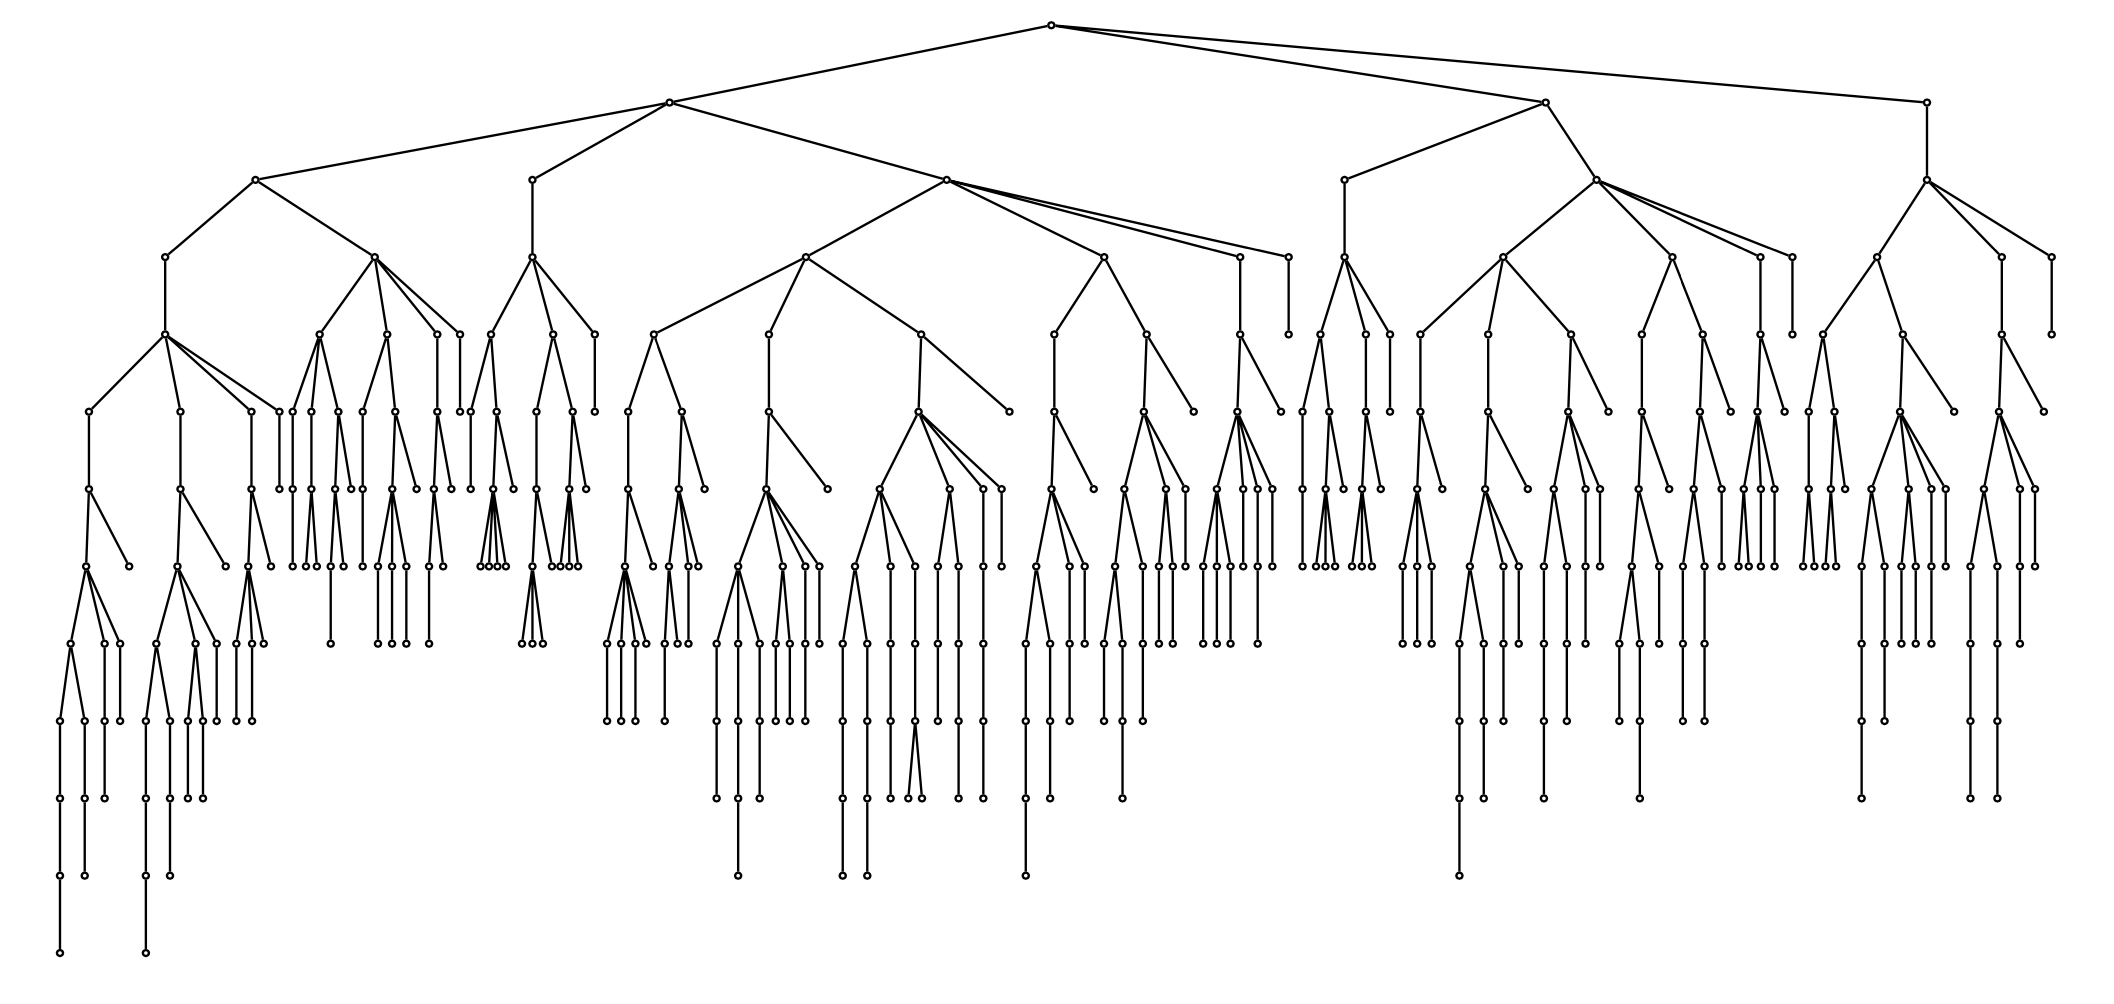
\includegraphics[width=14cm]{GRAPHICS/ON_POLY/schreier_tree_6}
$$
\caption{\label{fig:onpoly:schreier:tree:6}A Schreier tree in the action on polynomials}
\end{figure}
This particular orbit has length $420,$ so there are that many nodes in the tree.

\bigskip


%Suppose we want to draw the set of points in a graphical representation of the plane.
%The following command produces a picture of an ellitic curve shown earlier in Figure~\ref{fig:EC_11_1_3}.
%\begin{verbatim}
%orbiter.out -v 2 -process_combinatorial_objects -q 11 -n 2  \
%  -draw_points_in_plane EC_11_1_3 \
%  -fname_base_out EC_11_1_3 -embedded \
%  -input -file_of_points elliptic_curve_b1_c3_q11.txt -end \
%  -end
%\end{verbatim}
Orbiter can be used to create raytracing 3D-graphics.
Orbiter serves as a front end for the raytracing software Povray~\cite{povray}.
This is a multi step process: 
A 3D scene is defined through orbiter commands. 
Next, Orbiter produces Povray files. 
After that, the 
povray files are processed through povray, and turned into graphics files (png), called frames. 
The frames can be turned into a video 
by using tools like ffmpeg (see Section~\ref{sec:animations}).
By default, an rotational animation is produced. 

\bigskip

The Orbiter Povray interface requires some general information about the animation, 
the camera position, the boundary box for clipping, 
the font size for text and others.
Tables~\ref{tab:povray1}-~\ref{tab:povray2} list the commands to control the 3D-povray frontend.
\begin{table}
\begin{center}
\begin{tabular}{|p{4cm}|p{3cm}|p{7cm}|}
\hline
Command & Arguments & Purpose \\
\hline
\hline
\verb'-do_not_rotate' &  & No rotation. By default, the animation consists of a full rotation around a vertical axis.\\
\hline  
\verb'-rotate_about_' \verb'z_axis' &  & Rotate around $z$-axis. \\
\hline  
\verb'-rotate_about_111' &  & Rotate around $(1,1,1)$-axis (default). \\
\hline  
\verb'-rotate_about_' \verb'custom_axis' & axis & Rotate around a custom axis. The axis is specified as a vector of length 3. \\
\hline  
\verb'-boundary_none' &  & Remove the clipping. \\
\hline  
\verb'-boundary_box' &  & Clip using a box shape. \\
\hline  
\verb'-boundary_sphere' &  & Clip using a sphere (default). \\
\hline  
\verb'-font_size' & $s$  & Set font size to $s.$ \\
\hline  
\verb'-stroke_width' & $s$  & Set text depth to $s$. \\
\hline  
\verb'-omit_bottom_plane' &  & Remove the bottom plane. \\
\hline  
\verb'-W' & $w$ & Set output dimension to $w$ pixels wide. \\
\hline  
\verb'-H' & $h$ & Set output dimension to $h$ pixels height. \\
\hline  
\verb'-nb_frames' & $n$ & Set number of frames to $n$. One revolution around the axis is split into $n$ frames. \\
\hline  
\verb'-zoom' & $r$ $a_s$ $a_t$ $c_s$ $c_t$ & Set zoom angle and clipping with in round $r$ to change from $a_s$ to $a_t$ and from $c_s$ to $c_t$, respectively. \\
\hline  
\verb'-pan' & $r$ $F$ $T$ $C$ & In round $r$, pan the camera from location $F$ to location $T$ in a rotational movement with center at $C$. Each of $F,T,C$ are three dimensional coordinates.\\
\hline  
\verb'-pan_reverse' & $r$ $F$ $T$ $C$ & Same as \verb'-pan', but camera movement is in opposite order. \\
\hline  
\verb'-no_background' &  & Remove background. \\
\hline  
\verb'-no_bottom_plane' & $r$ & Remove bottom plane in round $r$. \\
\hline  
\verb'-camera' & $r$ $S$ $C$ $L$ & In round $r$, set camera location at $C$, sky at $S$ and pointing towards $L$. Each of $S,C,L$ are three-dimensional coordinate vectors. \\
\hline  
\end{tabular}
\end{center}
\caption{\label{tab:povray1}Options for Orbiter 3D-graphics (Part 1)}
\end{table}
\begin{table}
\begin{center}
\begin{tabular}{|p{4cm}|p{3cm}|p{7cm}|}
\hline
Command & Arguments & Purpose \\
\hline
\hline
\verb'-clipping' & $r$ $c$ & In round $r$, set clipping radius to $c$. \\
\hline  
\verb'-text' & $r$ $a$ text & In round $r$, produce running text \verb'text'  with sustain value $a$. \\
\hline  
\verb'-label' & $r$ $s$ $a$ $g$ text & In round $r$, produce running text \verb'text' with start value $s$, sustain $s$ and gravity $g$.  \\
\hline  
\verb'-latex' & $r$ $s$ $a$ praeamble $g$ text $l$ fname & In round $r$, produce running latex text \verb'text' with start value $s$, sustain $s$ and gravity $g$. Put \verb'praeamble' in the latex source code. Use \verb'fname' for the latex file names (no extension). \\
\hline  
\verb'-global_picture_' \verb'scale' & $d$ & Set scaling factor to $d$. \\
\hline  
\verb'-picture' & $r$ $d$ fname options & In round $r$, place picture \verb'fname' scaled by $d$ using options. \\
\hline  
\verb'-picture' & $r$ $d$ fname options & In round $r$, place picture \verb'fname' scaled by $d$ using options. \\
\hline  
\verb'-look_at' & $L$ & Override camera look-at value to $L$. $L$ is a three-dimensional vector. \\
\hline  
\verb'-default_angle' & $a$ & Set default camera angle to $a$. \\
\hline  
\verb'-clipping_radius' & $f$ & Set default clipping radius to $f$. \\
\hline  
\verb'-scale_factor' & $s$ & Set default scale factor to $s$. \\
\hline  
\verb'-line_radius' & $s$ & Set default line radius to $s$. \\
\hline  
\end{tabular}
\end{center}
\caption{\label{tab:povray2}Options for Orbiter 3D-graphics (Part 2)}
\end{table}
The main part in a 3D graphics is the scene desription. This tells the system what will be in the picture. 
A scene is composed of objects. Various types of objects are available: 
points, lines, planes, faces, algebraic surfaces, reguli, 3D-text,  
and others.
Some complex objects are predefined, for instance the Hilbert, Cohn-Vossen surface. 
Once the objects are defined, output commands can be invoked to draw them in various colors and with various options.
At times, there are many objects in one scene. In order to make drawing easier, it is possible to group objects. 
All objects in a group must have the same type. 
One group of object can be drawn with one command.
Tables~\ref{tab:scene1} and~\ref{tab:scene2} summarize the Orbiter commands to build objects of a 3D scene.
\begin{table}
	\begin{center}
	\begin{tabular}{|p{4.5cm}|c|p{8cm}|}
		\hline
		Command & Arguments & Purpose \\
		\hline
		\hline
		\verb'-cubic_lex' & coeffs & Cubic surface given by 20 coefficients in lexicographic ordering \\
		\hline
		\verb'-cubic_orbiter' & coeffs & Cubic surface given by 20 coefficients in Orbiter ordering \\
		\hline
		\verb'-cubic_Goursat' & $A$ $B$ $C$ & Cubic surface with tetrahedral symmetry given by 3 Goursat coefficients as $Axyz + B(x^2+y^2+z^2)+C=0$ \\
		\hline
		\verb'-quadric_lex_10' & coeffs & Quadric surface given by 10 coefficients in lexicographic ordering \\
		\hline
		\verb'-quartic_lex_35' & coeffs & Quartic surface given by 35 coefficients in lexicographic ordering \\
		\hline
		\verb'-octic_lex_165' & coeffs & Octic surface given by 165 coefficients in lexicographic ordering \\
		\hline
		\verb'-point' & coeffs & Point given by three coordinates \\
		\hline
		\verb'-point_list_' \verb'from_csv_file' & fname & List of points with coordinates given in a csv file \\
		\hline
		\verb'-line_through_two_' \verb'points_recentered_' \verb'from_csv_file' & fname & List of lines through two points with point coordinates given in a csv file \\
		\hline
		\verb'-line_through_two_' \verb'points_from_csv_file' & fname & List of lines through two points with point coordinates given in a csv file \\
		\hline
		\verb'-point_as_inter' \verb'section_of_two_lines' & $i_1$ $i_2$  & Create a point from the intersection of two lines $i_1$ and $i_2$ \\
		\hline
		\verb'-edge' & $i_1$ $i_2$  & Create an edge (line segment) between points $i_1$ and $i_2$ \\
		\hline
		\verb'-text' & $i_1$ $s$  & Create a label $s$ located at the point $i$  \\
		\hline
		\verb'-triangular_face_' \verb'given_by_three_lines' & $i_1$ $i_2$ $i_3$  & Create a triangular face give by three lines $i_1,i_2,i_3$ \\
		\hline
		\verb'-face' & pts  & Create a face through the vertices pts, ordered cyclically \\
		\hline
		\verb'-quadric_through_' \verb'three_skew_lines' & $i_1$ $i_2$ $i_3$  & Create a quadric through three skew lines \\
		\hline
		\verb'-plane_defined_by_' \verb'three_points' & $i_1$ $i_2$ $i_3$  & Create a plane through three noncollinear points \\
		\hline
		\verb'-line_through_two_' \verb'points_recentered' & pt-coords   & Create a line through two points given by 6 coordinates, recentered \\
		\hline
		\end{tabular}
	\end{center}
	\caption{\label{tab:scene1}Scene definition commands (part 1)}
	\end{table}
	\begin{table}
	\begin{center}
	\begin{tabular}{|p{4.5cm}|c|p{8cm}|}
		\hline
		Command & Arguments & Purpose \\
		\hline
		\hline
		\verb'-line_through_two_' \verb'points' & pt-coords   & Create a line through two points given by 6 coordinates \\
		\hline
		\verb'-line_through_two_' \verb'existing_points' & $i_1$ $i_2$   & Create a line through two points \\
		\hline
		\verb'-line_through_' \verb'point_with_direction' & $x$ $y$ $z$ $u_x$ $u_y$ $u_z$   & Create a line through a point $(x,y,z)$ with a given direction $(u_x,u_y,u_z)$ \\
		\hline
		\verb'-plane_by_dual_' \verb'coordinates' & $a$ $b$ $c$ $d$   & Create the plane $ax+by+cz+d=0$ given in dual coordinates \\
		\hline
		\verb'-dodecahedron' &    & Create a Dodecahedron centered at the origin (20 points, 30 edges, 12 faces) \\
		\hline
		\verb'-Hilbert_Cohn_' \verb'Vossen_surface' &    & Create the Hilbert, Cohn-Vossen surface (1 cubic surface, 45 tritangent planes, 27 lines) \\
		\hline
		\verb'-obj_file' &  fname  & Read points and faces from the given .obj file \\
		\hline
		\verb'-group_of_' \verb'things' &  list  & Create a group of things from the given list \\
		\hline
		\verb'-group_of_' \verb'things_with_offset' &  list offset & Create a group of things from the given list, each value is increase by offset \\
		\hline
		\verb'-group_of_' \verb'things_as_interval' &  $a$ $b$ & Create a group of things indexed by the interval $a, \ldots, a+b -1$ \\
		\hline
		\verb'-group_of_' \verb'things_as_interval_' \verb'with_exceptions' &  $a$ $b$ ex & Create a group of things indexed by the interval $a, \ldots, a+b -1$ with the exceptional elements in the list ex removed\\
		\hline
		\verb'-group_of_all_points' &   & Create a group of things from all points currently defined\\
		\hline
		\verb'-group_of_all_faces' &   & Create a group of things from all faces currently defined\\
		\hline
		\verb'-group_subset_' \verb'at_random' & $i$ $f$  & Create a group of things from the existing group $i$ by picking a random subset with probability $f$ \\
		\hline
		\verb'-create_regulus' & $i$ $N$  & Create a regulus for quadric $i$ with $N$ lines \\
		\hline
		\end{tabular}
	\end{center}
	\caption{\label{tab:scene2}Scene definition commands (part 2)}
	\end{table}
Building the scene itself does not create any graphical output. 
To this end, the commands in Table~\ref{tab:3doutput} are used.
Each of these commands applies to a group of objects of the same kind. 
Groups of objects are created using the commands in 
Table~\ref{tab:scene2} which start with \verb'group_of'.
	\begin{table}
	\begin{center}
	\begin{tabular}{|p{4.5cm}|c|p{8cm}|}
		\hline
		Command & Arguments & Purpose \\
		\hline
		\hline
		\verb'-spheres' & $i$ $r$ prop & For each element in point group $i$, create a sphere of radius $r$ with given Povray properties.\\
		\hline
		\verb'-cylinders' & $i$ $r$ prop & For each element in edge group $i$, create a cylinder of radius $r$ with given Povray properties.\\
		\hline
		\verb'-prisms' & $i$ $d$ prop & For each element in face group $i$, create a prism of half-thickness $d$ with given Povray properties.\\
		\hline
		\verb'-planes' & $i$ prop & For each element in plane group $i$, create a plane with given Povray properties.\\
		\hline
		\verb'-lines' & $i$ $r$ prop & For each element in line group $i$, create a line of radius $r$ with given Povray properties.\\
		\hline
		\verb'-cubics' & $i$ prop & For each element in group $i$ of cubics, create a surface with given Povray properties.\\
		\hline
		\verb'-quadrics' & $i$ prop & For each element in group $i$ of quadrics, create a surface with given Povray properties.\\
		\hline
		\verb'-quartics' & $i$ prop & For each element in group $i$ of quartics, create a surface with given Povray properties.\\
		\hline
		\verb'-octics' & $i$ prop & For each element in group $i$ of octics, create a surface with given Povray properties.\\
		\hline
		\verb'-texts' & $i$ $d$ $s$ prop & For each element in group $i$ of labels, create a text element with half-thickness $d$ and size $s$ with given Povray properties.\\
		\hline
		\end{tabular}
	\end{center}
	\caption{\label{tab:3doutput}Graphical output commands}
	\end{table}
Here is a simple example which combines scene building and graphical output.
The example creates a cube with vertices, edges and faces:
{\tt
\input GRAPHICS/THE_MAKEFILE/EXTRACTS/cube.tex
}
This command instructs Orbiter to create 30 povray files (extension .pov), 
one for each frame of a rotating scene. 
The scene containes a cube whose vertices are shown in chrome, 
whose edges are in red, and whose faces are yellow and transparent. 
The cube turns around a vertical axis of symmetry.
Here is the first frame of the result:
$$
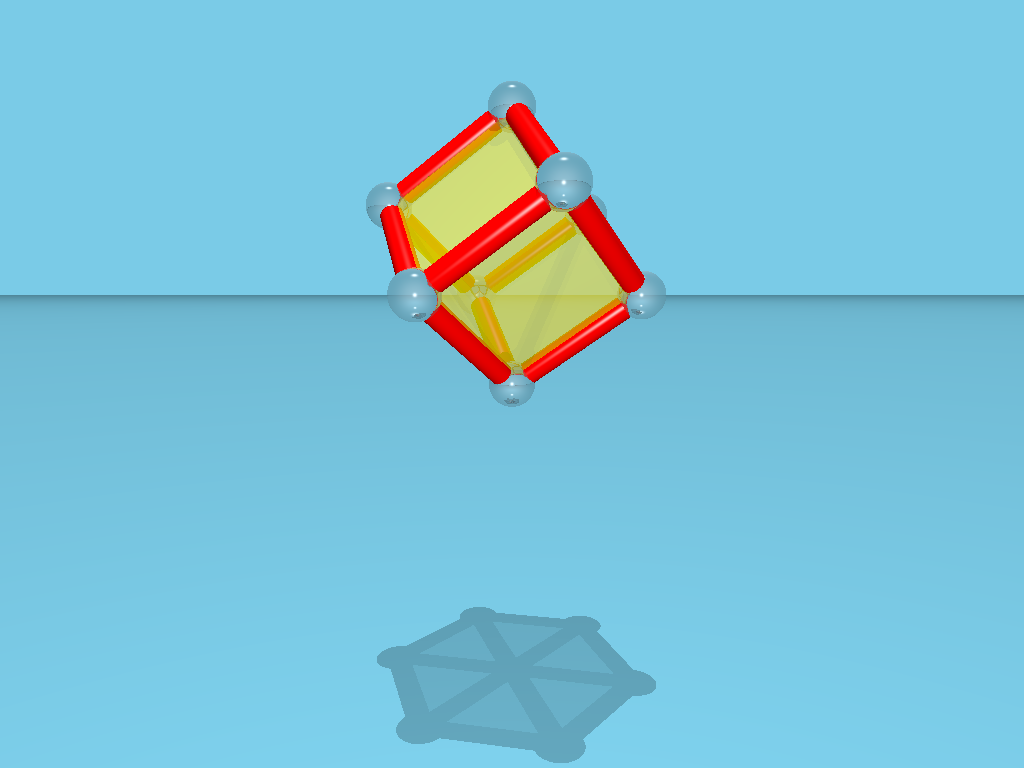
\includegraphics[width=9cm]{GRAPHICS/POVRAY/cube_0_000}
$$
The coordinates of the cube are stored in an object file \verb'cube_centered.obj'.
The content of this file is:
\begin{verbatim}
v -1 -1 -1 
v 1 -1 -1 
v -1 1 -1 
v 1 1 -1 
v -1 -1 1 
v 1 -1 1 
v -1 1 1 
v 1 1 1 
f 1 2 4 3
f 1 2 6 5 
f 1 3 7 5 
f 2 4 8 6 
f 3 4 8 7 
f 5 6 8 7
\end{verbatim}
The monkey saddle is a cubic surface, given by the equation 
$$
z = x^3-3xy^2
$$
The next example plots the surface knowns as the monkey saddle. 
The tangent plane at $(0,0,0)$ is drawn as well. 
An animation is created by rotating the scene around the $z$-axis.
{\tt
\input GRAPHICS/THE_MAKEFILE/EXTRACTS/MONKEY_SADDLE_CUBIC.tex
}
{\tt
\input GRAPHICS/THE_MAKEFILE/EXTRACTS/monkey.tex
}
Here is one of the frames that are created:
$$
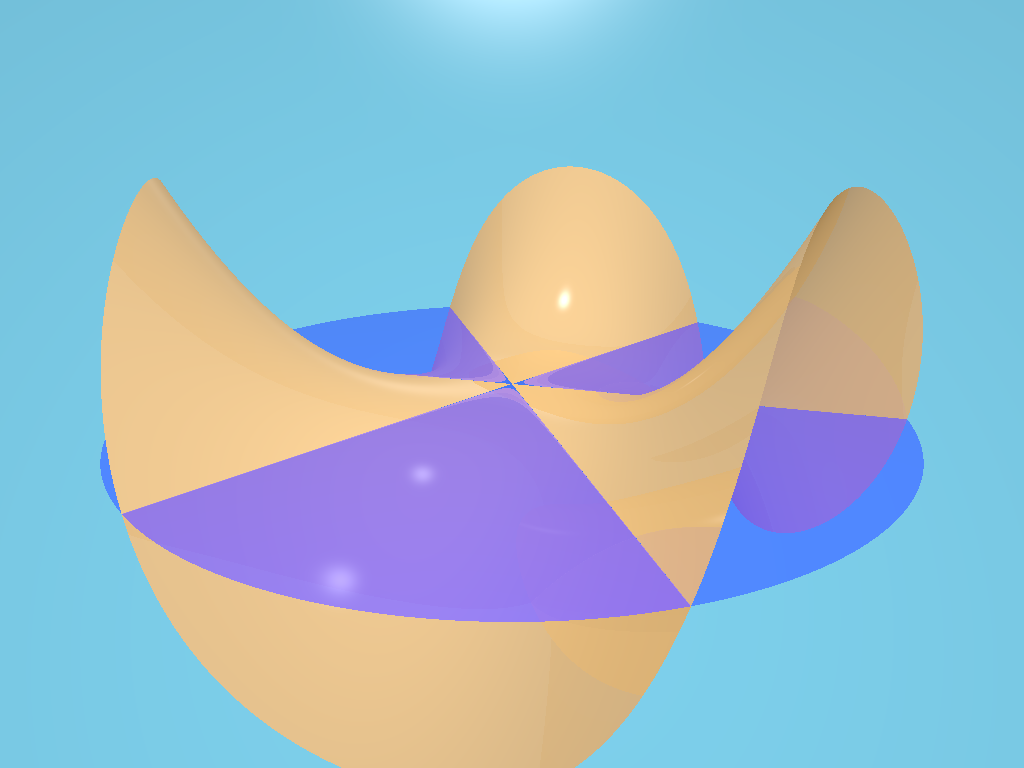
\includegraphics[width=9cm]{GRAPHICS/POVRAY/monkey_0_000}
$$
The Eckardt surface is given by the equation
$$
\frac{5}{2}xyz-(x^2+y^2+z^2)+1=0.
$$
We use the following code to plot the surface and the lines on it. 
The Schl\"afli labeling of the lines is indicated.
{\tt
\input GRAPHICS/THE_MAKEFILE/EXTRACTS/Eckardt.tex
}
Figure~\ref{fig:HCV} shows the final product. 
\begin{figure}
$$
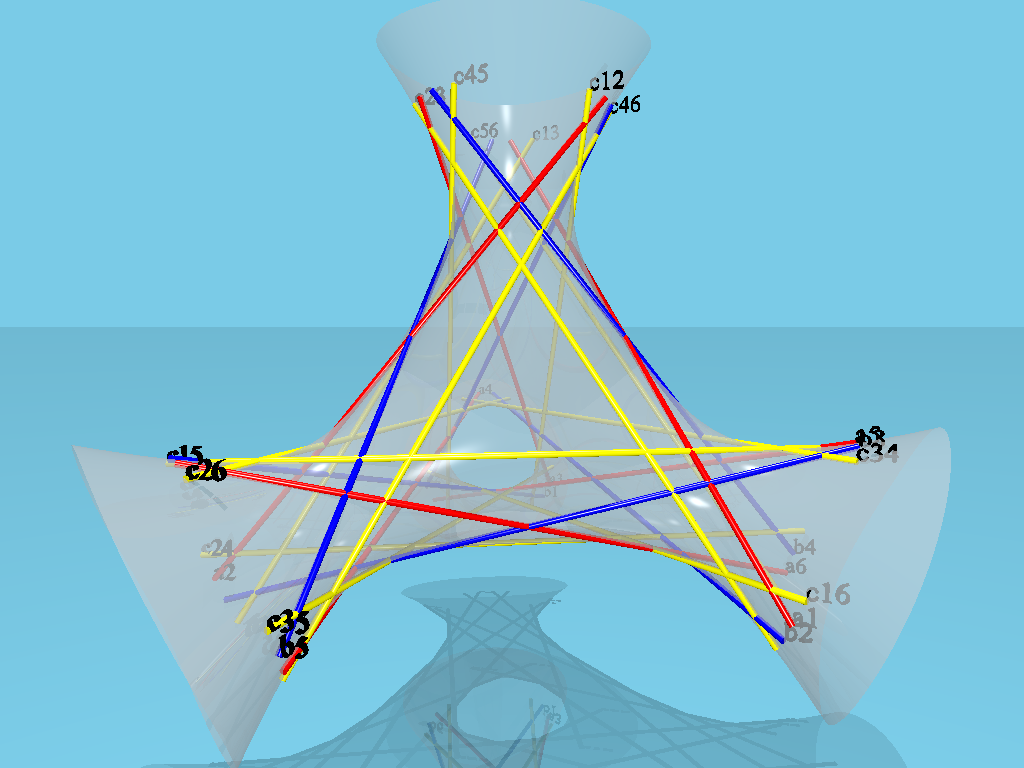
\includegraphics[width=15cm]{GRAPHICS/POVRAY/HCV_0_029}
$$
\caption{\label{fig:HCV}The Eckardt surface}
\end{figure}





\bigskip

The Endrass octic~\cite{Endrass97} is the algebraic surface given by the equation
$$
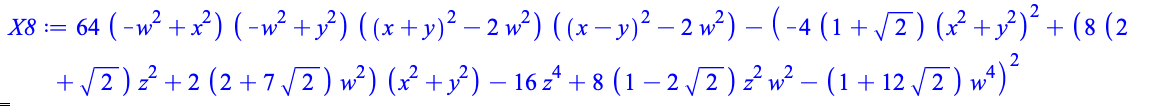
\includegraphics[width=15cm]{GRAPHICS/POVRAY/X8_as_given}
$$
The following Orbiter command creates a povray graphics of the octic, shown in Figure~\ref{fig:octic}:
{\tt
\input GRAPHICS/THE_MAKEFILE/EXTRACTS/ENDRASS_OCTIC_LEX_165.tex
}
{\tt
\input GRAPHICS/THE_MAKEFILE/EXTRACTS/endrass8.tex
}
\begin{figure}
$$
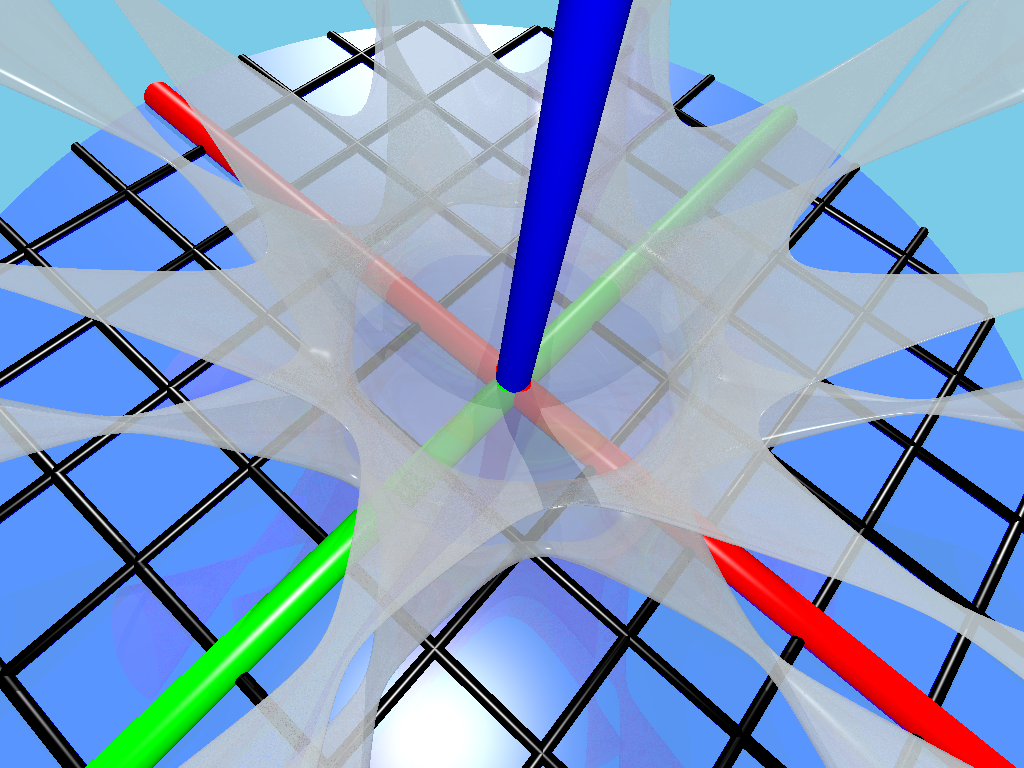
\includegraphics[width=9cm]{GRAPHICS/POVRAY/endrass_octic_0_004}
$$
\caption{\label{fig:octic}The Endrass Octic}
\end{figure}
This illustration includes coordinate axes and the $x,y$-plane. 

\bigskip

Orbiter can be used to create animations. 
This relies on the software \verb'ffmpeg'.
In a first step, all frames (i.e. individual graphics files) are created using Orbiter's povray interface. 
After that, the frames are used to create the animation. 
In order to use \verb'ffmpeg', the frames should have a uniform file naming scheme, 
using a consecutive numbering to arrange the files in order. 
This is achieved by using a printf style mask, with \verb'%d' representing the number of the current frame.
In order to do so, Orbiter can be used to copy and rename files. 
A temporary directory can be used to collect the files.
The Orbiter command \verb'perpare_frames' can be used. For a list of commands, see Tables~\ref{tab:prepareframes}.
	\begin{table}
	\begin{center}
	\begin{tabular}{|p{4.5cm}|c|p{8cm}|}
		\hline
		Command & Arguments & Purpose \\
		\hline
		\hline
		\verb'-i' & $s$ $l$ mask & Specify the input file names 
by running a printf command with the given mask applied to the index $i$ where $i$ goes from $s$ to $s+l-1.$ This option can be repeated. \\
		\hline
		\verb'-step' & $s$  & Increment the index in steps of size $s$. \\
		\hline
		\verb'-o' & mask & Create the output file using the given mask.\\
		\hline
		\verb'-output_starts_at' & $i$ & Start output file indices at $i$ (default is 0).\\
		\hline
		\end{tabular}
	\end{center}
	\caption{\label{tab:prepareframes}Prepare frames commands}
	\end{table}
For instance, the command 
{\tt
\input GRAPHICS/THE_MAKEFILE/EXTRACTS/monkey_video.tex
}
creates a video \verb'monkey.mp4' from a set of 30 files. The individual 
filenames are created using the printf format string \verb'monkey_0_%03d.png', 
with an integer index that is drawn from the interval $[0,29].$ 
The part that starts with a percent sign and ends with a ``d'' character
defines the way in which the integer is formatted. 
The number three before the ``d'' indicates 
that three characters will be printed. 
The zero indicates the use of leading zeros.
So, the first file would be \verb'monkey_0_000.png' 
and the very last file is \verb'monkey_0_029.png'. 
The description of the printf format string can be found in the 
documentation of the C standard library~\cite{KernighanRitchie78}.
Orbiter can plot functions using a built-in function tracker.
The functions must be continuous apart from a finite number of poles.
The function can have multiple components, each described using an expression. 
Each expression is specified in Reverse Polish Notation (RPN).
Consider an example. 
A Lissajous curve is defined using coordinate functions of the form 
$$
x = r \sin\big(at + c\big), \quad
y = r \sin\big(bt\big), \quad a,b,c,r \in \bbR.
$$
The terms 
$$
r \sin\big(at + c\big), \quad r \sin\big(bt\big)
$$
are the expressions of the two coordinate functions.
RPN means that the operator is listed after the operands. 
A stack data structure is used to hold temporary values. 
Operators are pushed to the top of the stack using the push commands.
A binary operator pops the two elements from the stack, performs the operation, 
and pushes the resulting value back onto the stack. 
For a unary operator, only one element is popped and replaced by the result.
Here are some examples of expressions rewritten in RPN:
\begin{align*}
\sin(x) &\mapsto \; \mbox{push} \; x \; \sin,\\
a+b & \mapsto \; \mbox{push} \; a \; \mbox{push} \; b \; \mbox{add},\\
a\cdot b & \mapsto \; \mbox{push} \; a \; \mbox{push} \; b \; \mbox{mult}.
\end{align*}
The coordinate functions are enclosed between \verb'-code' and \verb'-code_end' commands. 
Each coordinate function is described in RPN and terminated using a \verb'return' keyword.
By the time the \verb'return' keyword is reached, the RPN expression must have exactly 
one value on the stack which is considered the value of the expression.
Constants are declared between the \verb'-const' and \verb'-const_end' keywords. 
Likewise, variables are declared between the \verb'-var' and \verb'-var_end' keywords.
Picking $a=3$, $b=2,$ $c = \pi/2$ and $r=7$, the function is computed using 
{\tt
\input GRAPHICS/THE_MAKEFILE/EXTRACTS/lissajous.tex
}
The sequence
$$
\verb'push t push a mult push c add sin push r mult'
$$
is $r\sin(at+c)$ expressed in RPN.
The constants are defined in the line 
$$
\verb'-const a 3 b 2 c 1.57 r 7 -const_end'
$$
The input variable is defined using the line 
$$
\verb'-var t -var_end'
$$
The sequence 
$$
\verb'-smooth_curve "lissajous" 0.07 2000 15 0 18.85'
$$
defines the name of the output file, the fact that two consecutive 
points are never further than $\epsilon =0.07$ away, 
the fact that points that are 15 or more away from the origin should be ignored, 
and the fact that the variable $t$ loops over the range $[0,18.85]$ 
with a default of $2000$ steps.
The evaluator automatically reduces the step-size 
if consecutive image points are more than $\epsilon$ apart.  
The code to produce the plot is
{\tt
\input GRAPHICS/THE_MAKEFILE/EXTRACTS/lissajous_plot.tex
}
The plot is shown in Figure~\ref{fig:lissajous}.
\begin{figure}
$$
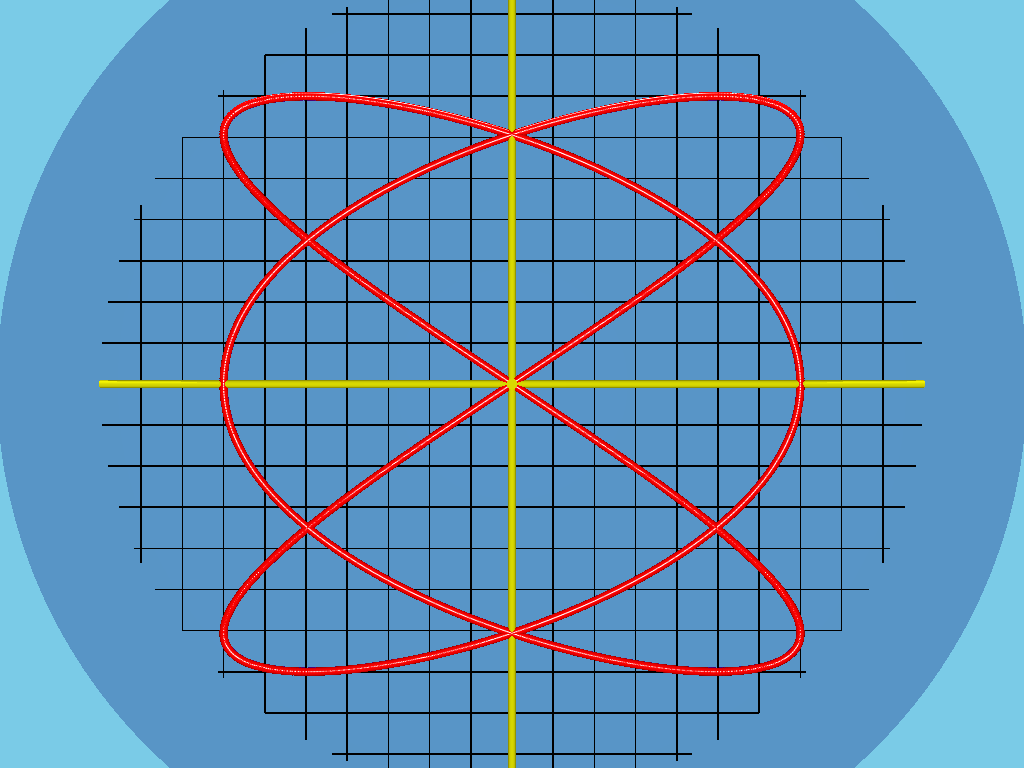
\includegraphics[width=9cm]{GRAPHICS/POVRAY/lissajous_0_000}
$$
\caption{\label{fig:lissajous}Lissajous figure}
\end{figure}


\bigskip


We can turn it into a 3D plot by using the $t$ value for the $z$ coordinate. 
The 
function is computed using the command 
{\tt
\input GRAPHICS/THE_MAKEFILE/EXTRACTS/lissajous_3d.tex
}
The code to produce the 3D plot is
{\tt
\input GRAPHICS/THE_MAKEFILE/EXTRACTS/lissajous_3d_plot.tex
}
The 3D curve is shown in Figure~\ref{fig:lissajous3d}.
\begin{figure}
$$
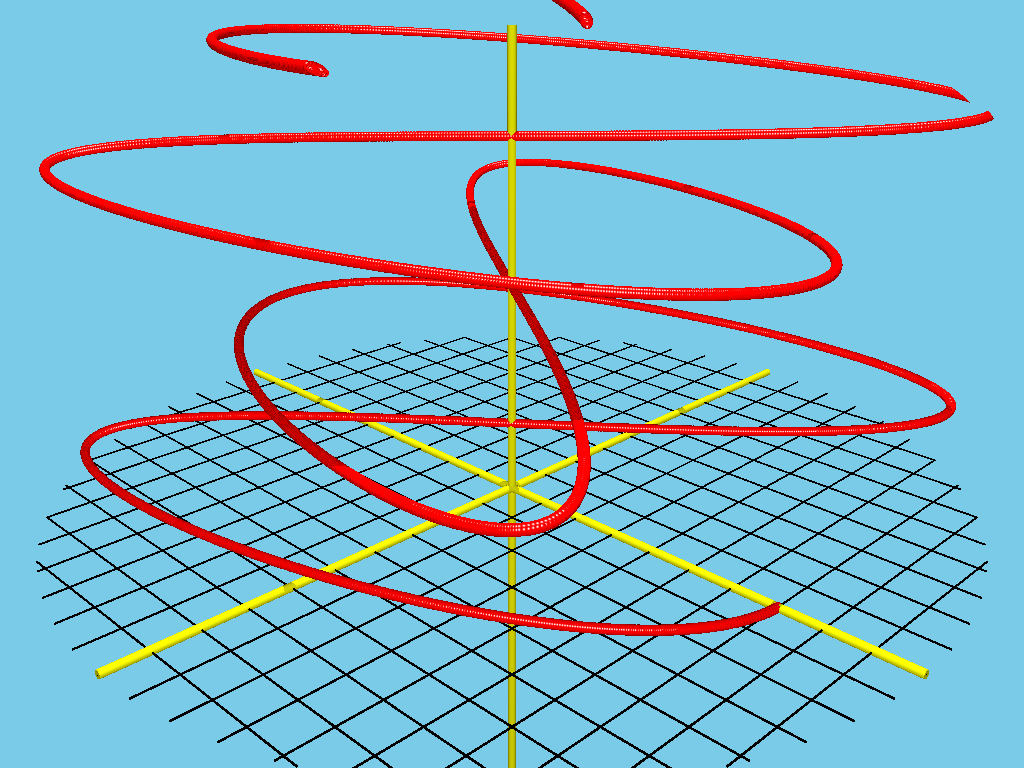
\includegraphics[width=9cm]{GRAPHICS/POVRAY/lissajous_3d_0_000}
$$
\caption{\label{fig:lissajous3d}Lissajous Spacecurve}
\end{figure}
\section{Miscellaneous}
\label{sec:miscellaneous}


\input C17/sec_1.tex



\bigskip

\clearpage



\section{Limitations}
\label{sec:limitations}


\input C17/sec_2.tex



\bigskip

\clearpage

Table~\ref{tab:misc} list miscellaneous Orbiter commands.
\begin{table}
\begin{center}
\begin{tabular}{|p{4cm}|p{3cm}|p{7cm}|}
\hline
Command & Arguments & Purpose \\
\hline
\hline
\verb'-csv_file_select_' \verb'rows' & fname $R$ & Selects rows listed in $R$ from the csv-file fname. \\
\hline  
\verb'-csv_file_select_' \verb'cols' & fname $R$ & Selects columns listed in $R$ from the csv-file fname. \\
\hline  
\verb'-csv_file_select_' \verb'rows_and_cols' & fname $R$ $C$ & Selects rows listed in $R$ and columns listed in $C$ from the csv-file fname. \\
\hline  
\verb'-csv_file_join' & fname col-label  & Joins csv file fname according to column with label col-label. This option is given once for each file that should be joined. \\
\hline  
\verb'-csv_file_latex' & fname   & Produces a latex table from the given csv-file. \\
\hline  
\verb'-store_as_csv_file' & fname $m$ $n$ $L$  & Stores the data in $L$ to a csv file. The data is an $m \times n$ matrix in row-major ordering. \\
\hline  
\end{tabular}
\end{center}
\caption{\label{tab:misc}Miscellaneous Orbiter Commands}
\end{table}
The command \verb'-csv_file_select_rows' can be used to select rows from a csv file. 
The command \verb'-csv_file_select_cols' can be used to select columns from a csv file. 
The command \verb'-csv_file_select_rows_and_cols' selects rows and columns. 
Here is an example. We create the multiplication table of the finite field $\bbF_7$, 
ordered according to the powers of a primitive element:
$$
\alpha^0, \alpha^1, \alpha^2, \alpha^3, \alpha^4, \alpha^5.
$$
After that, we pull the rows and columns corresponding to even powers $\alpha^0, \alpha^2, \alpha^4.$
{\tt
\input GRAPHICS/THE_MAKEFILE/EXTRACTS/misc_select.tex
}
The even powers of $\alpha$ create a multiplicative subgroup. 
Figure~\ref{fig:fieldtables7rearranged:selected} shows the table of the 
multiplicative group $\bbF_7^*$ and the subgroup of squares 
(compare with Figure~\ref{fig:fieldtables7rearranged} in Section~\ref{sec:finite:fields}).
\begin{figure}
$$
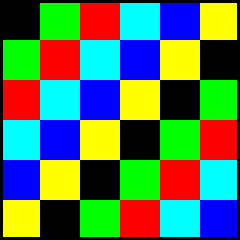
\includegraphics[width=5cm]{GRAPHICS/GF/GF_q7_multiplication_table_reordered_draw}
\qquad
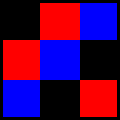
\includegraphics[width=5cm]{GRAPHICS/GF/GF_q7_multiplication_table_reordered_select_draw}
$$
\caption{\label{fig:fieldtables7rearranged:selected}Cyclic multiplication table 
of $\bbF_7$ and subgroup of squares}
\end{figure}
Here is the file \verb'GF_q7_multiplication_table_reordered.csv'
\begin{mdframed}[style=MyFrame]
\begin{verbatim}
Row,C0,C1,C2,C3,C4,C5
0,1,3,2,6,4,5
1,3,2,6,4,5,1
2,2,6,4,5,1,3
3,6,4,5,1,3,2
4,4,5,1,3,2,6
5,5,1,3,2,6,4
END
\end{verbatim}
\end{mdframed}
and next the file that is created by selecting rows and columns $0,2,4$:
\begin{mdframed}[style=MyFrame]
\begin{verbatim}
Row,"C0","C2","C4"
0,"1","2","4"
1,"2","4","1"
2,"4","1","2"
END
\end{verbatim}
\end{mdframed}

Several limitations exist in Orbiter. Here is a list:

\begin{enumerate}
\item
Field elements are encoded as  $\verb'int'$. This limits the size of fields that can be handled to $2^{8s-1}$ where $s=$\verb'sizeof(int)'.
\item
The ranks of elements in the permutation domain are encoded as  $\verb'long int'$. 
This limits the size of permutation domains that can be handled.
The degree of a permutation group must be less that $2^{8s-1}$ where $s=$\verb'sizeof(long int)'.
\item
The finite field class builds tables for the addition and multiplication of field elements. 
This restricts the size of the fields that can be created.
\item
The projective geometry class tries to build a bitmatrix for the adjacency matrix if the number of lines is less than 
\verb'MAX_NUMBER_OF_LINES_FOR_INCIDENCE_MATRIX' which is defined in \verb'src/lib/foundations/geometry/projective_space.cpp'. 
If the number of lines is too big, the table is not created. In this case, the projective geometry class may behave slower.
\item
The projective geometry class tries to build a table for the lines if the number of points is less that \verb'MAX_NUMBER_OF_POINTS_FOR_POINT_TABLE' and the number of 
lines is less than 
\verb'MAX_NUMBER_OF_LINES_FOR_LINE_TABLE', both of which are  defined in \verb'src/lib/foundations/geometry/projective_space.cpp'.
If the number of points is too big, the table is not created. In this case, the projective geometry class may behave slow.
\item
The projective geometry class tries to build a table for the lines through any two points if the number of points is less than 
\verb'MAX_NB_POINTS_FOR_LINE_THROUGH_TWO_POINTS_TABLE' which is defined in \verb'src/lib/foundations/geometry/projective_space.cpp'.
If the number of points is too big, the table is not created. In this case, the projective geometry class may behave slow.
\item
The projective geometry class tries to build a table for the intersection points of pairs of lines if the number of points is less than 
\verb'MAX_NB_POINTS_FOR_LINE_INTERSECTION_TABLE' which is defined in \verb'src/lib/foundations/geometry/projective_space.cpp'.
If the number of points or lines is too big, the table is not created. In this case, the projective geometry class may behave slow.
\item
For Windows users: Cygwin by default uses 32 bit integers for both \verb'int' and \verb'long int'. Using Cygwin 64 to compile Orbiter recommended.
\item
A limited list of primitive polynomials are hard-coded in Orbiter. For large fields, the user must provide their own primitive polynomial.
The polynomials encoded in orbiter are not guaranteed to be compatible with the subfield relationship.
%\item
%The base and strong generators used by Orbiter (see Section~\ref{sec:permutation:groups}) do not lead to optimal Schreier trees. 
%This is a performance issue for projective linear groups. The techniques of shallow Schreier trees (cf. Seress~\cite{Seress03}) 
%would be useful.
%\item
%Orbiter uses long integer arithmetic for the orders of finite groups, so there is no restriction in the order of finite groups from that point of view. 
\end{enumerate}
\section{Using Windows Subsystem Linux}



\input C18/sec_1.tex


\bigskip

\clearpage



The following quote from \url{https://docs.microsoft.com/en-us/windows/wsl/} 
summarizes the function of the Windows Subsystem for Linux:
\begin{quote}
Windows Subsystem for Linux (WSL) lets developers run a GNU/Linux environment -- 
including most command-line tools, utilities, and applications -- 
directly on Windows, unmodified, 
without the overhead of a traditional virtual machine or dual-boot setup.
You can:
\begin{enumerate}
\item
Choose your favorite GNU/Linux distributions from the Microsoft Store.
\item
Run common command-line tools such as grep, sed, awk, or other ELF-64 binaries.
\item
Run Bash shell scripts and GNU/Linux command-line applications including:
\item
Tools: vim, emacs, tmux
\item
Languages: NodeJS, Javascript, Python, Ruby, C/C++, C\# \& F\#, Rust, Go, etc.
\item
Services: SSHD, MySQL, Apache, lighttpd, MongoDB, PostgreSQL.
\item
Install additional software using your own GNU/Linux distribution package manager.
\item
Invoke Windows applications using a Unix-like command-line shell.
\item
Invoke GNU/Linux applications on Windows.
\end{enumerate}
\end{quote}

\bigskip


The following set of slides will ilustrate the installation of Orbiter under WSL.

\clearpage

$$

\includegraphics[width=15cm]{GRAPHICS/WIN/win1}
$$
$$
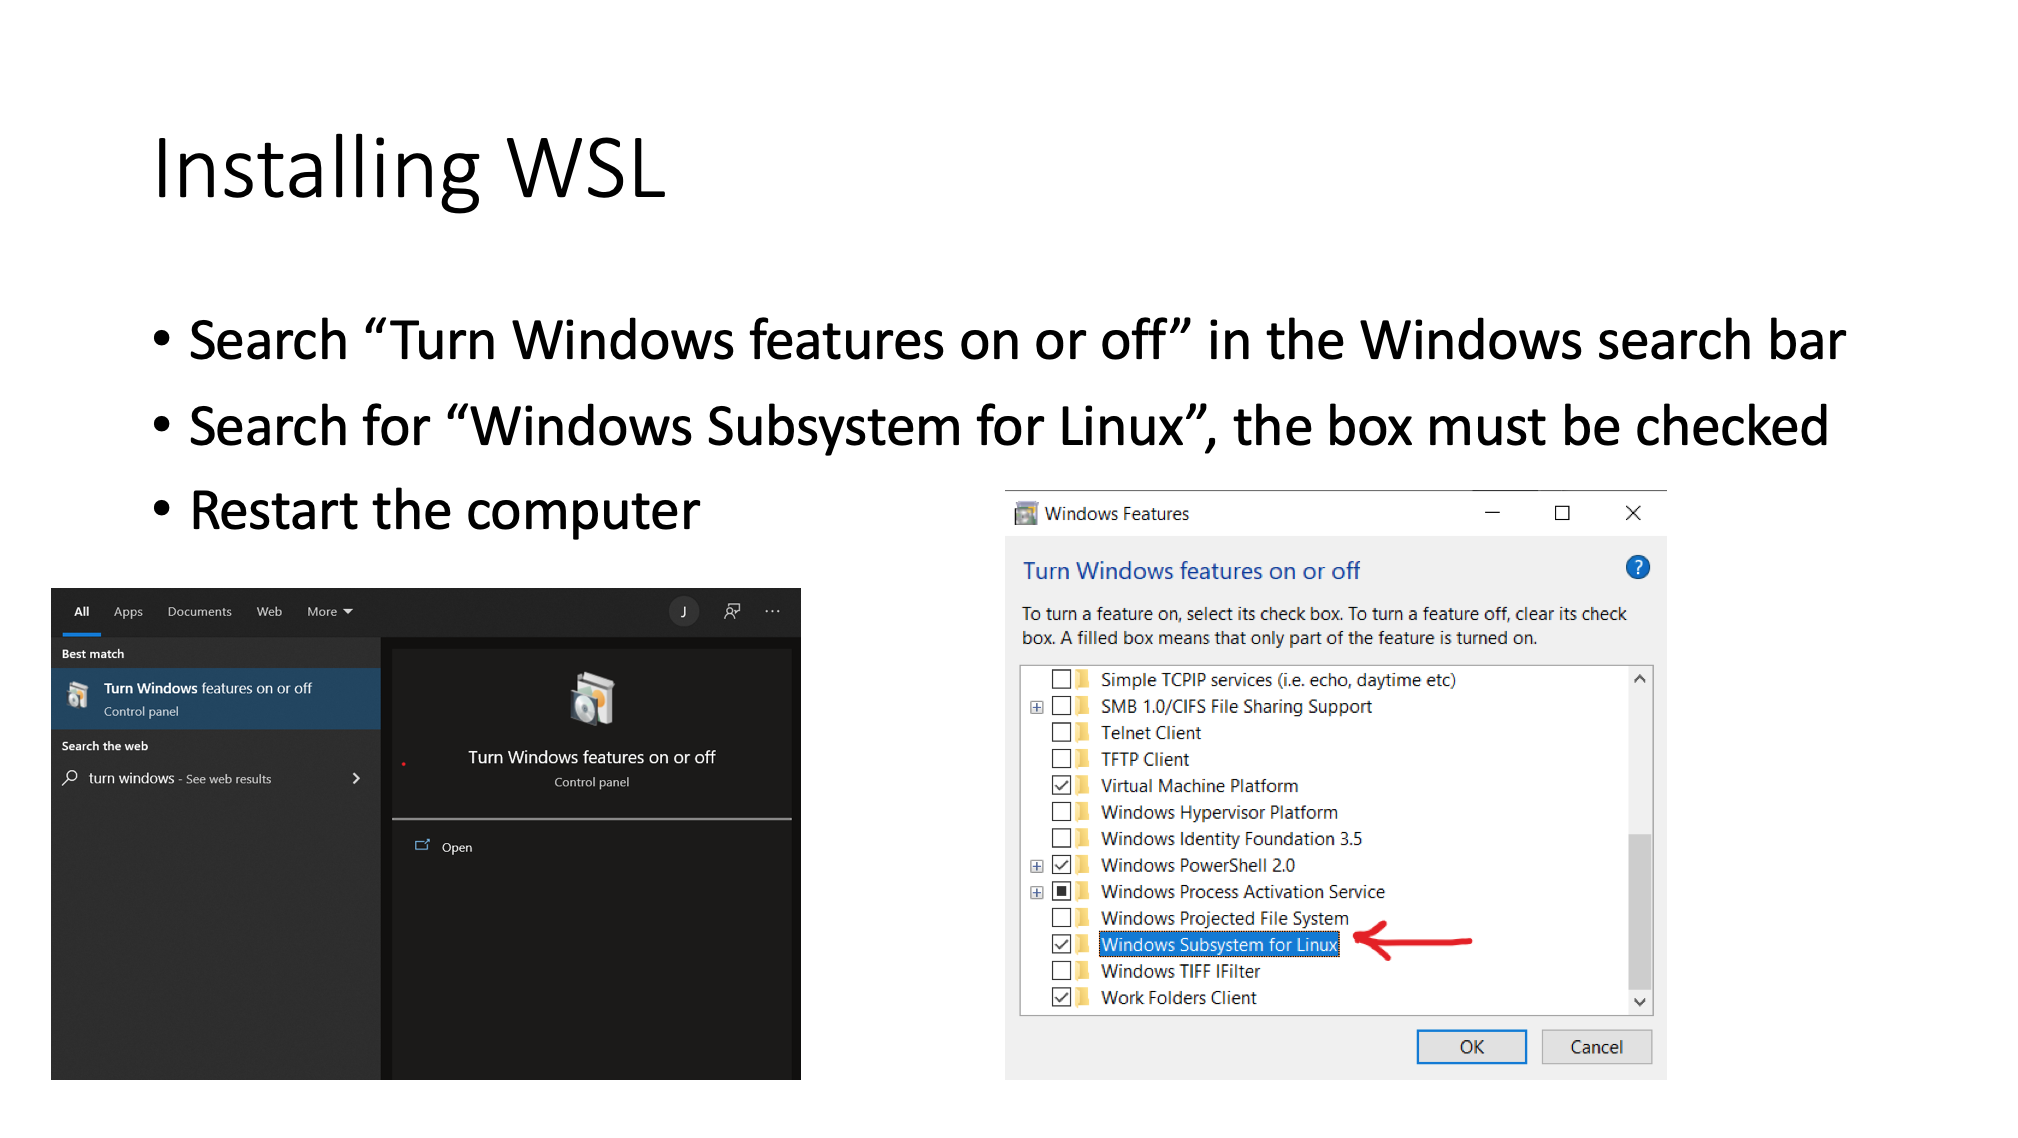
\includegraphics[width=15cm]{GRAPHICS/WIN/win2}
$$

\clearpage

$$
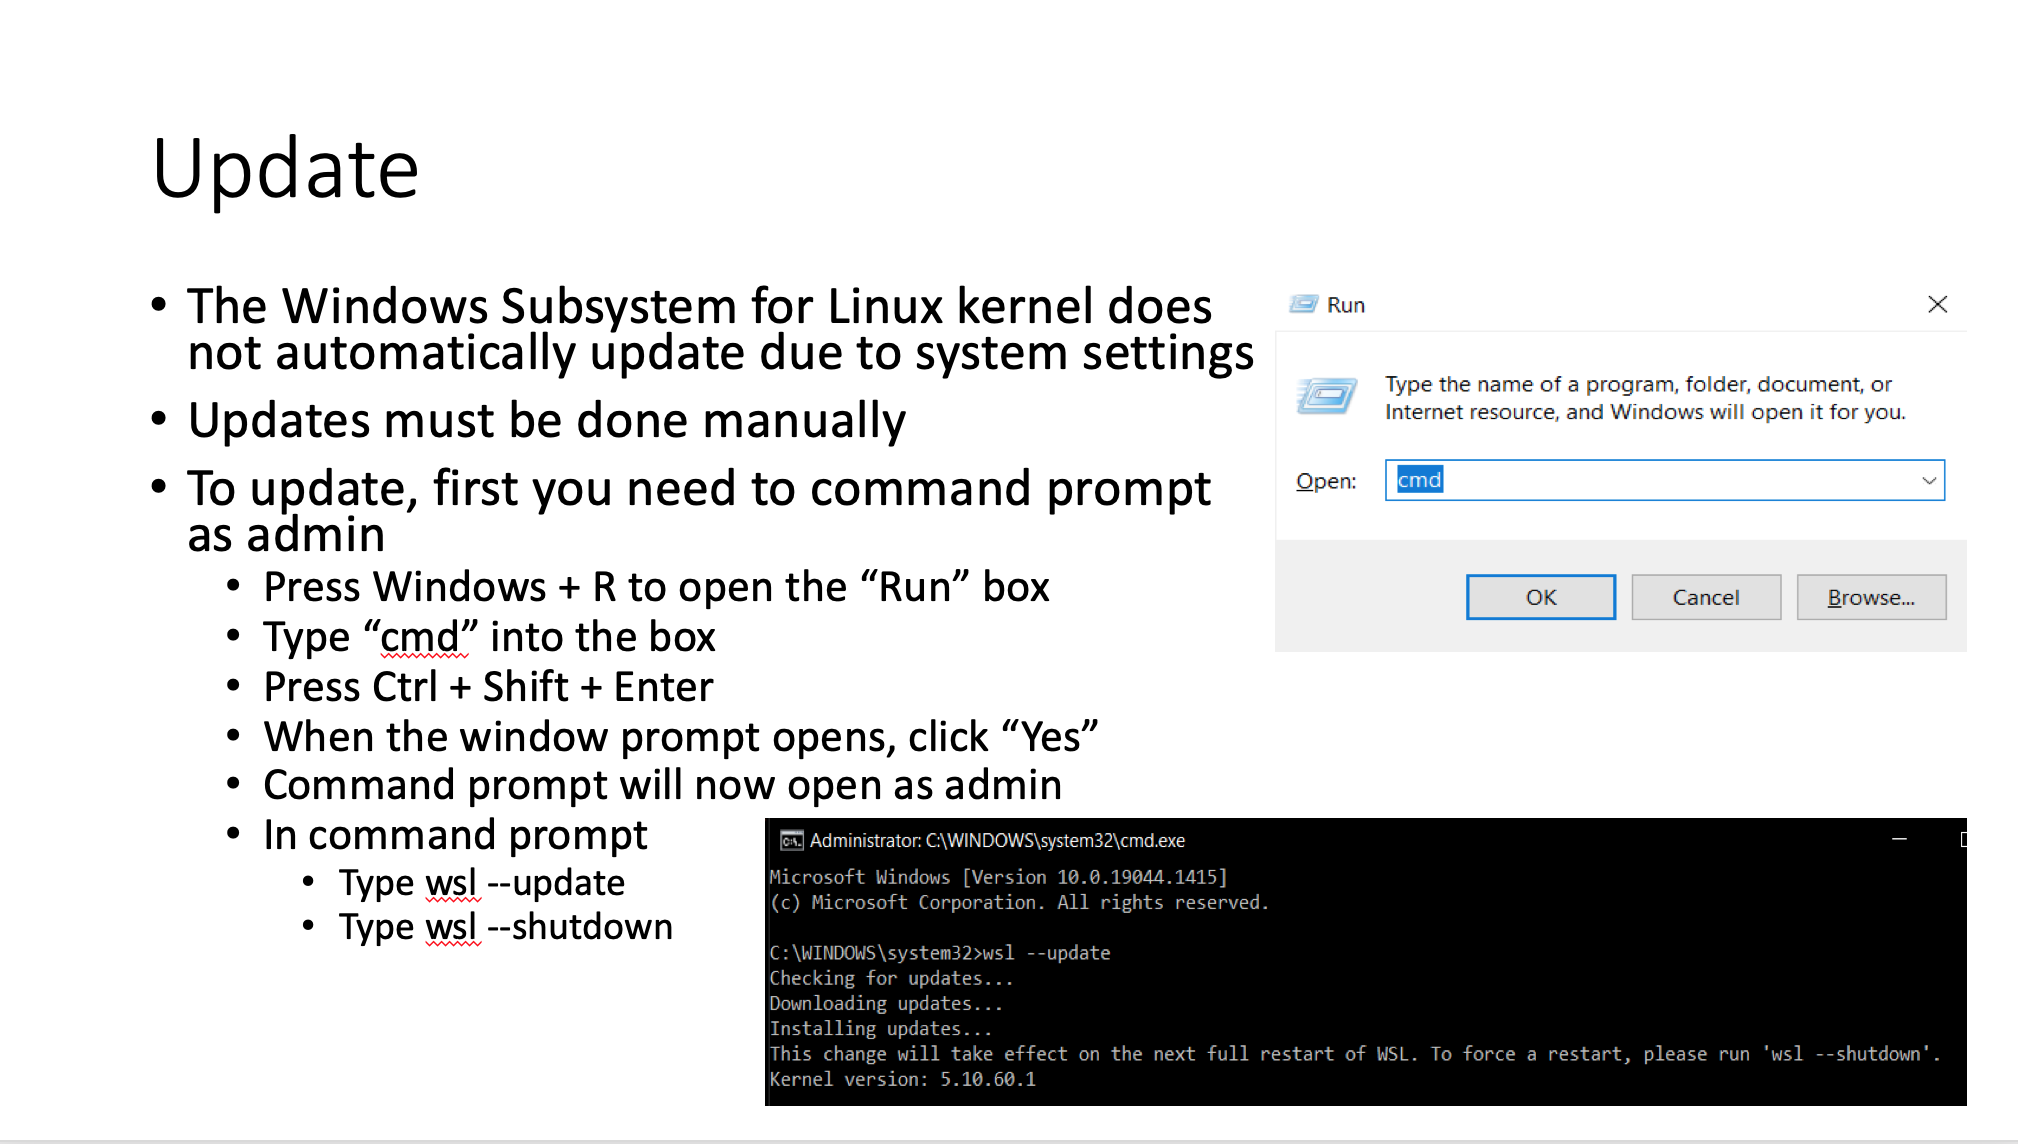
\includegraphics[width=15cm]{GRAPHICS/WIN/win3}
$$
$$
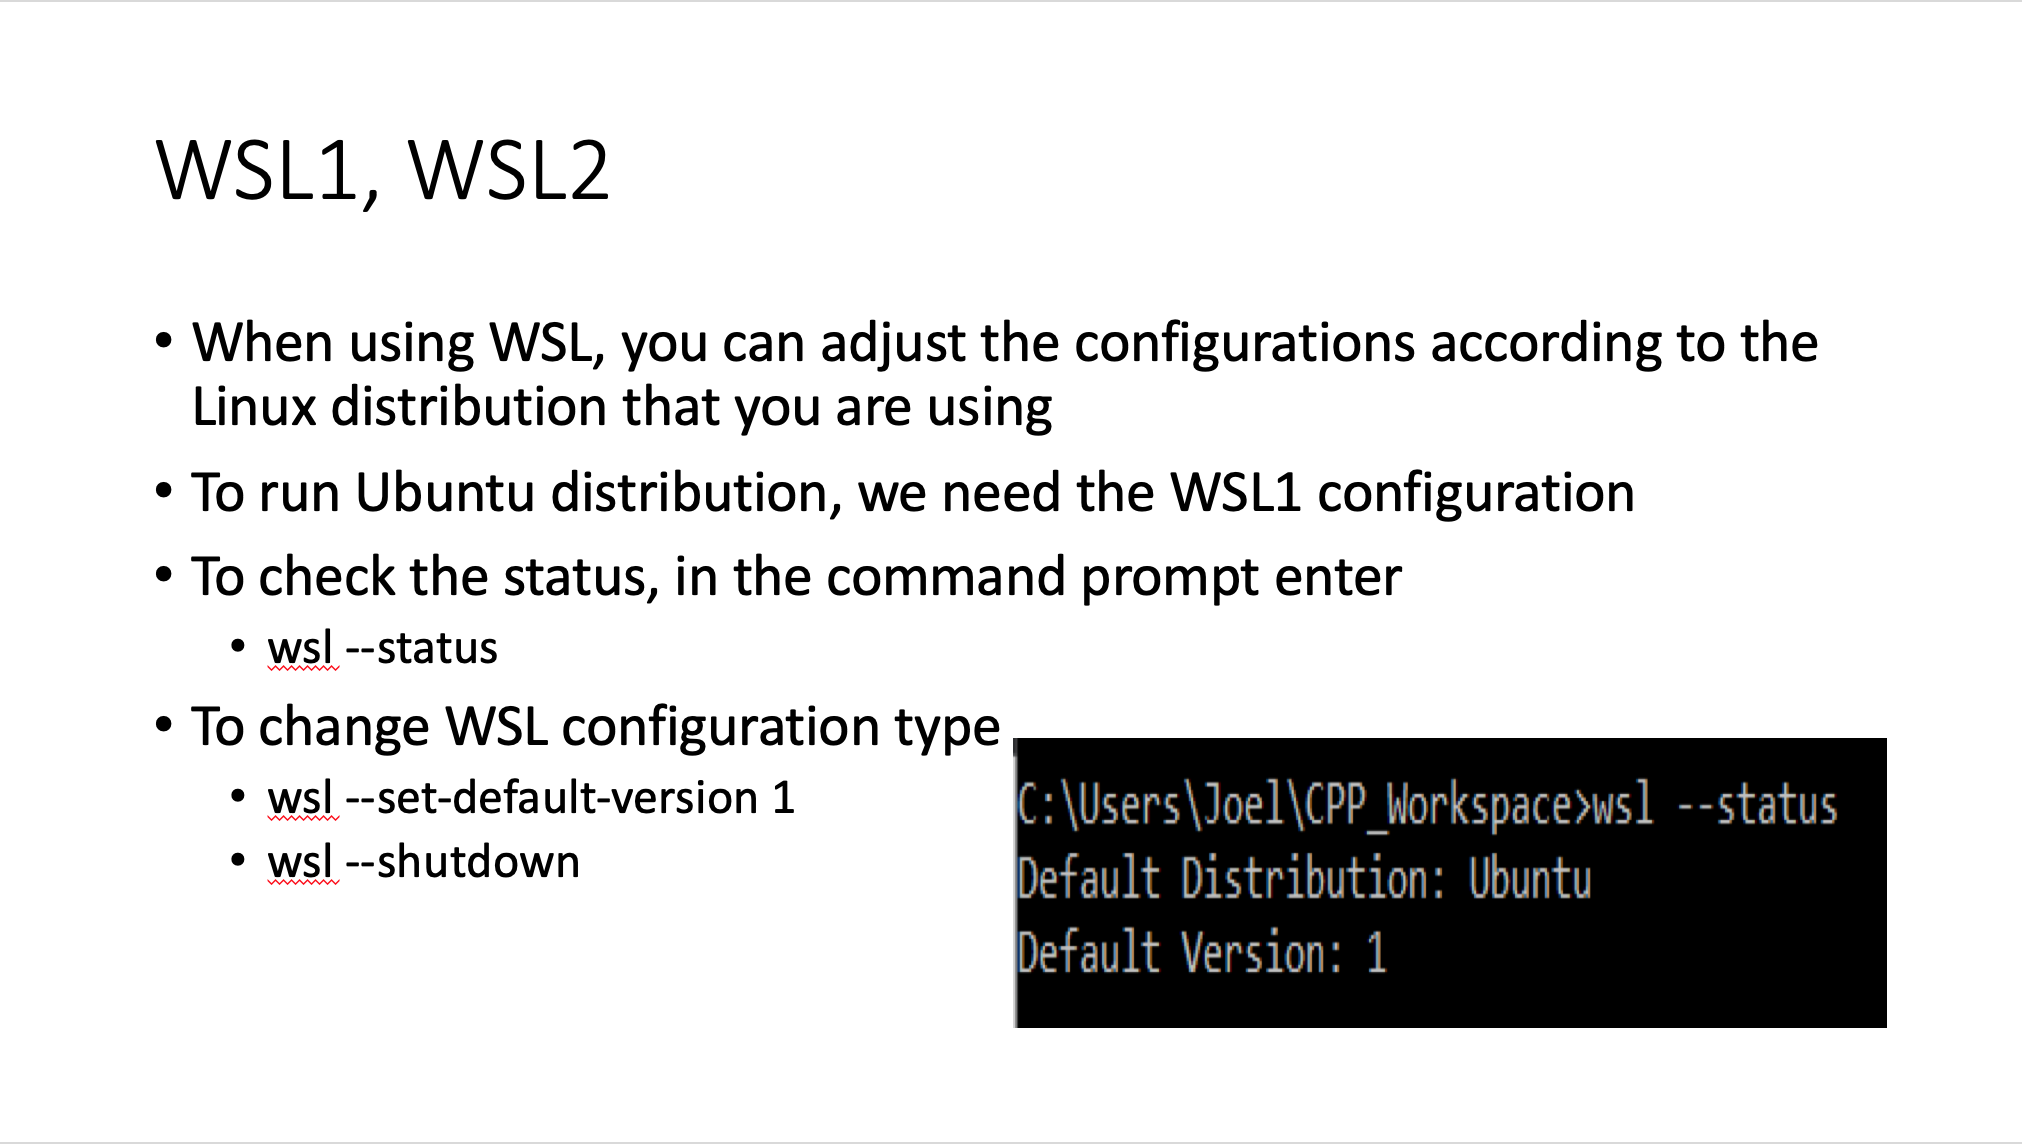
\includegraphics[width=15cm]{GRAPHICS/WIN/win4}
$$

\clearpage

$$
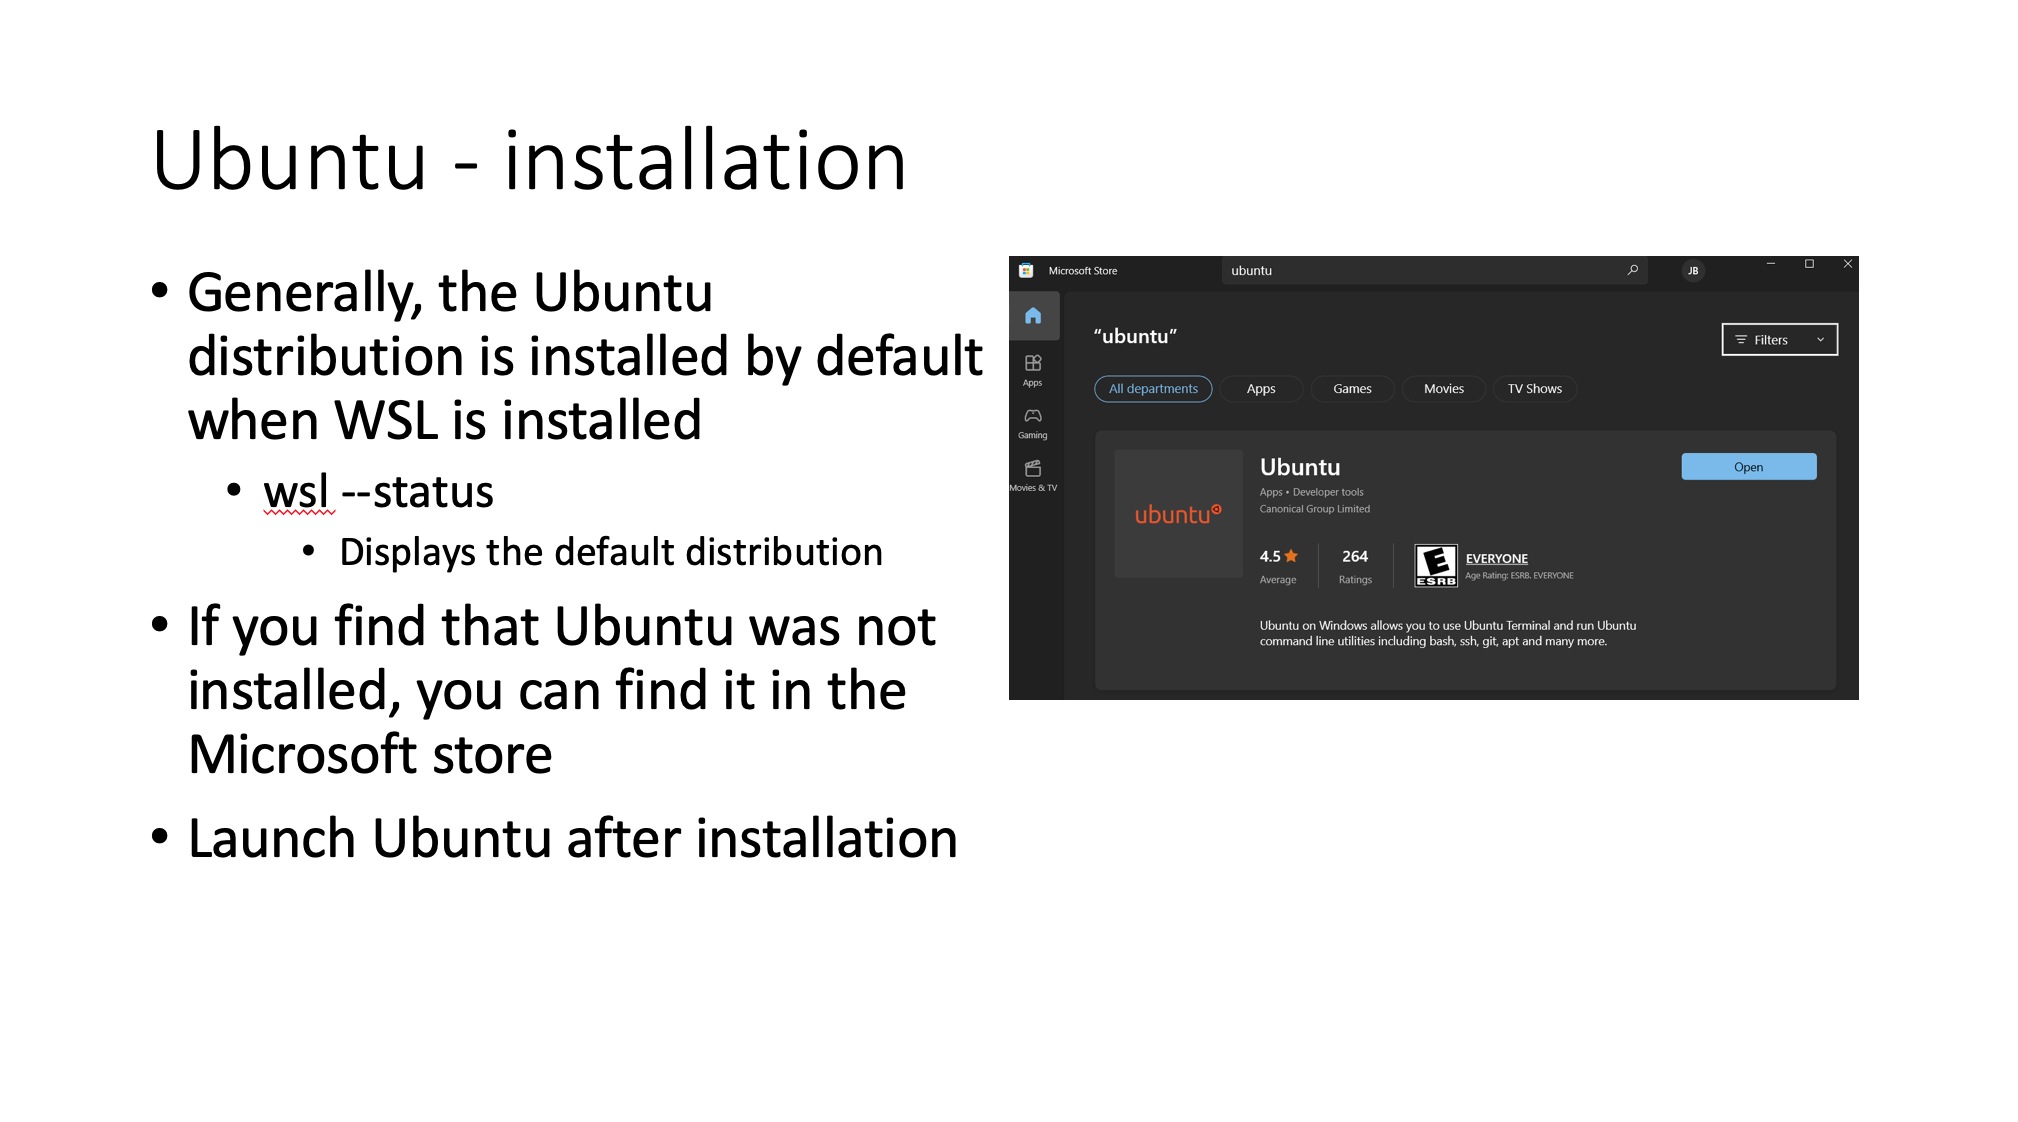
\includegraphics[width=15cm]{GRAPHICS/WIN/win5}
$$
$$
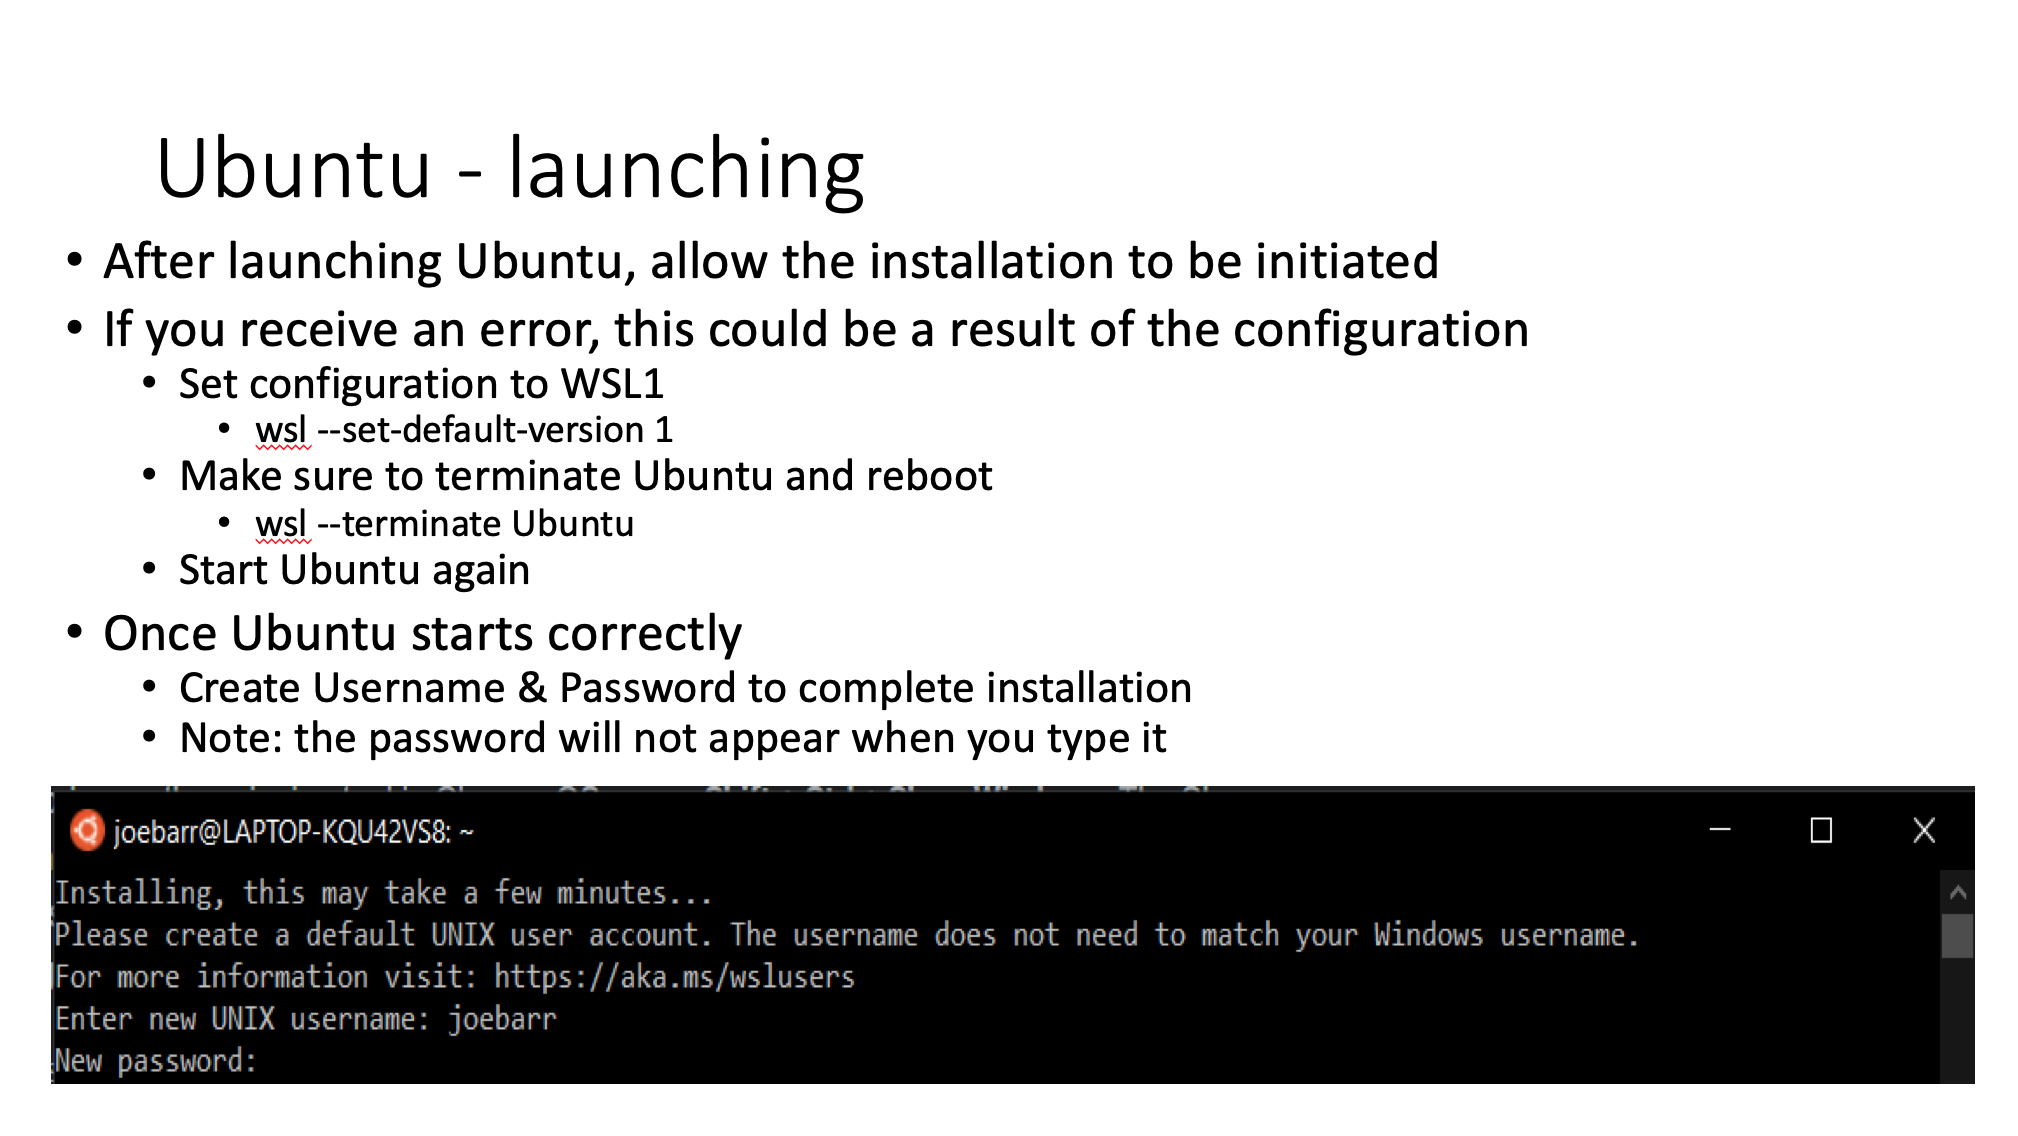
\includegraphics[width=15cm]{GRAPHICS/WIN/win6}
$$

\clearpage


$$
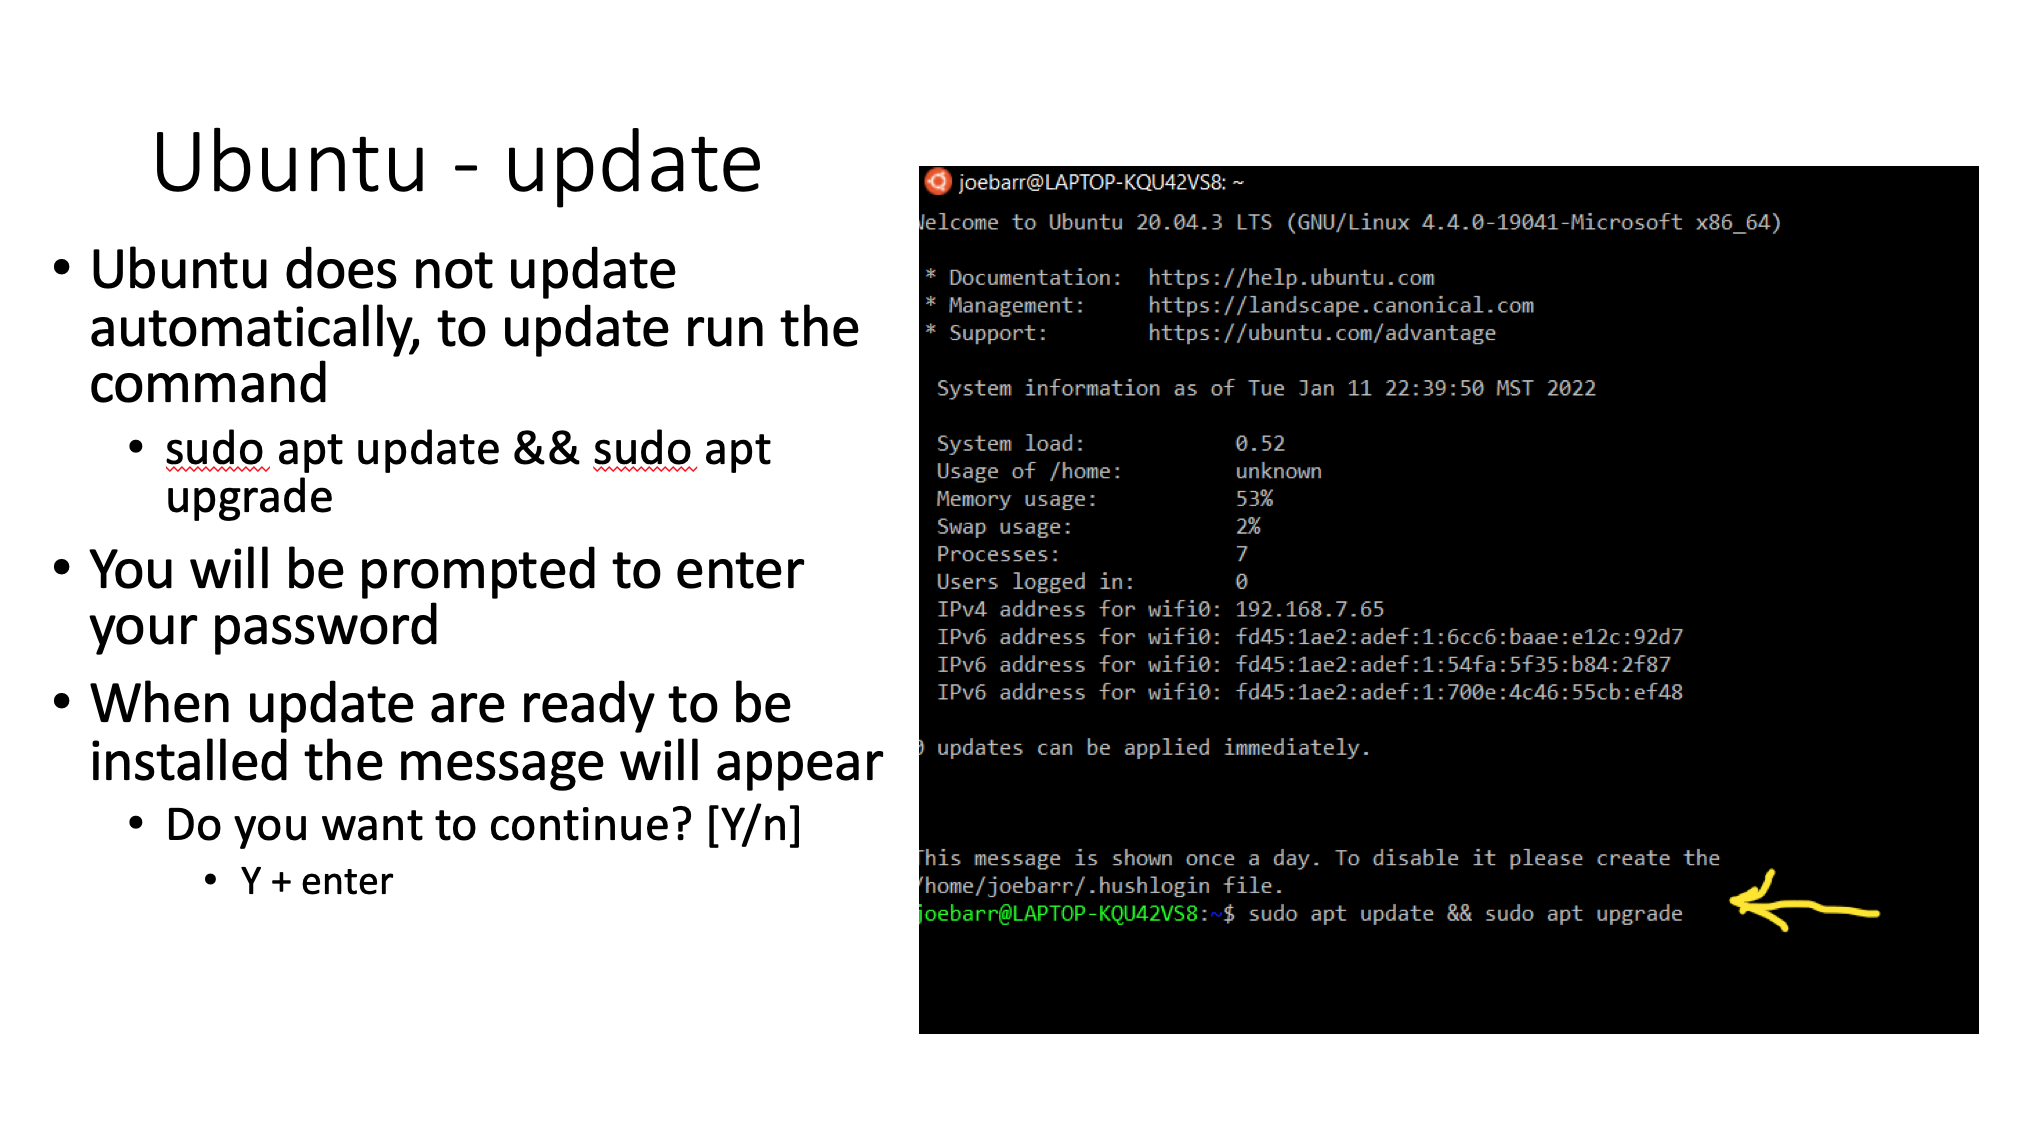
\includegraphics[width=15cm]{GRAPHICS/WIN/win7}
$$
$$
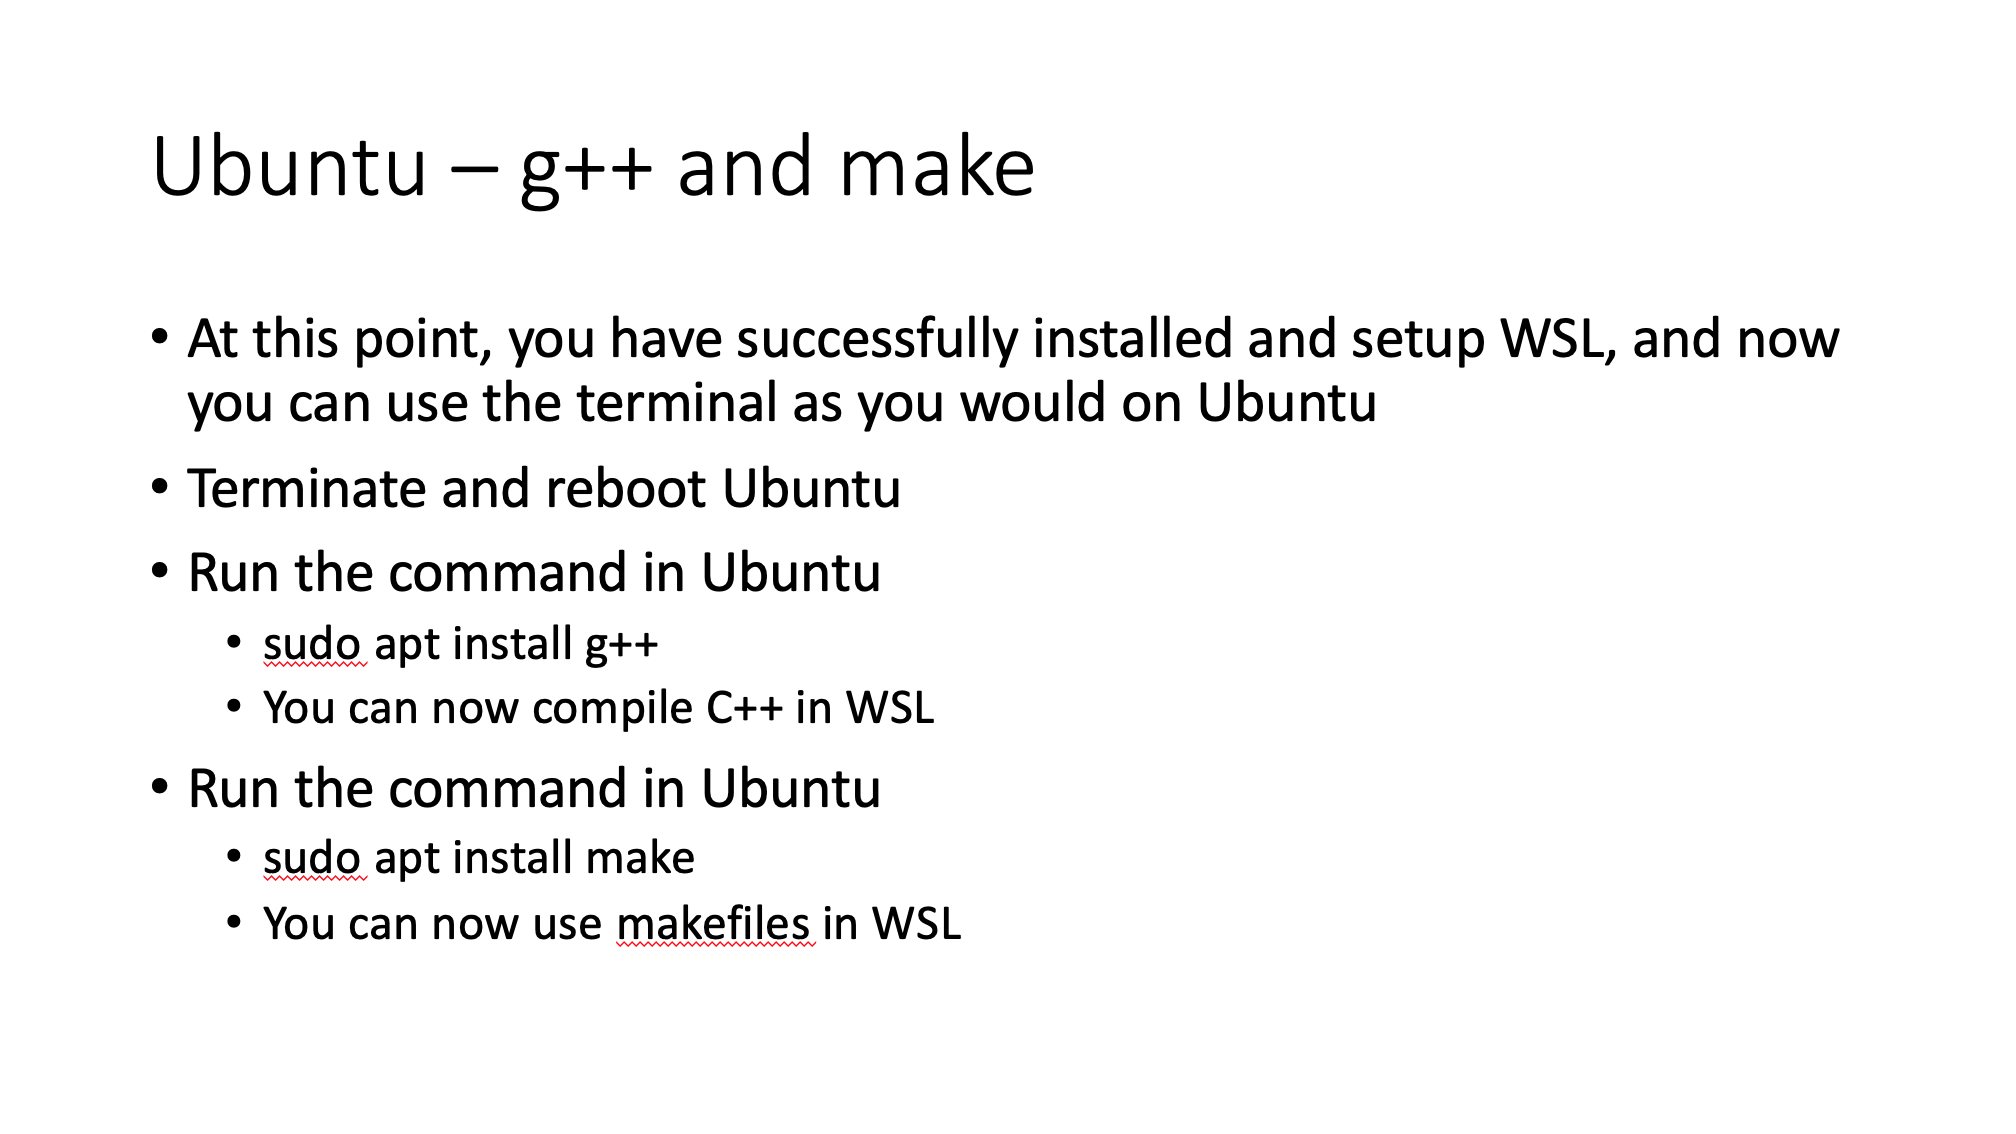
\includegraphics[width=15cm]{GRAPHICS/WIN/win8}
$$

\clearpage

$$
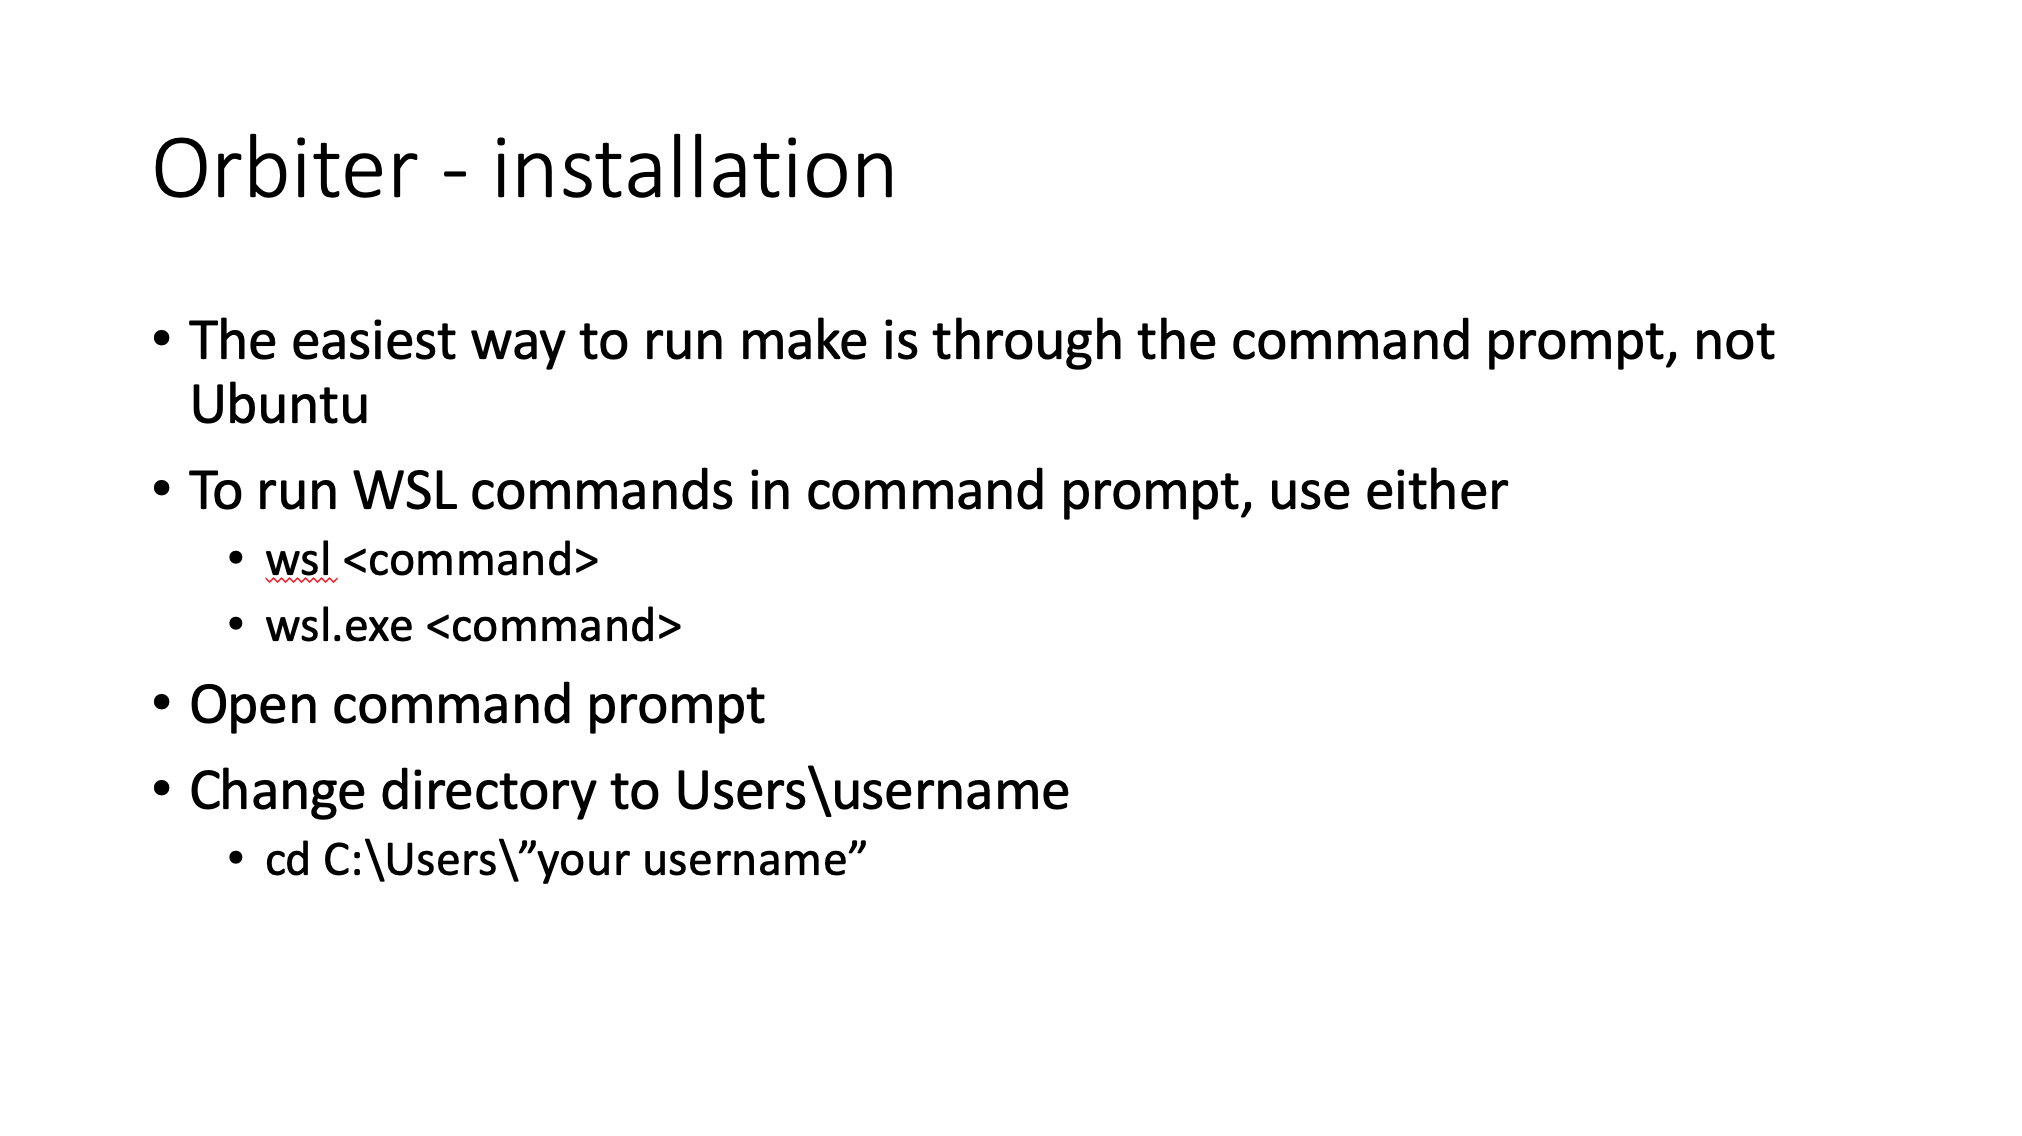
\includegraphics[width=15cm]{GRAPHICS/WIN/win9}
$$
$$
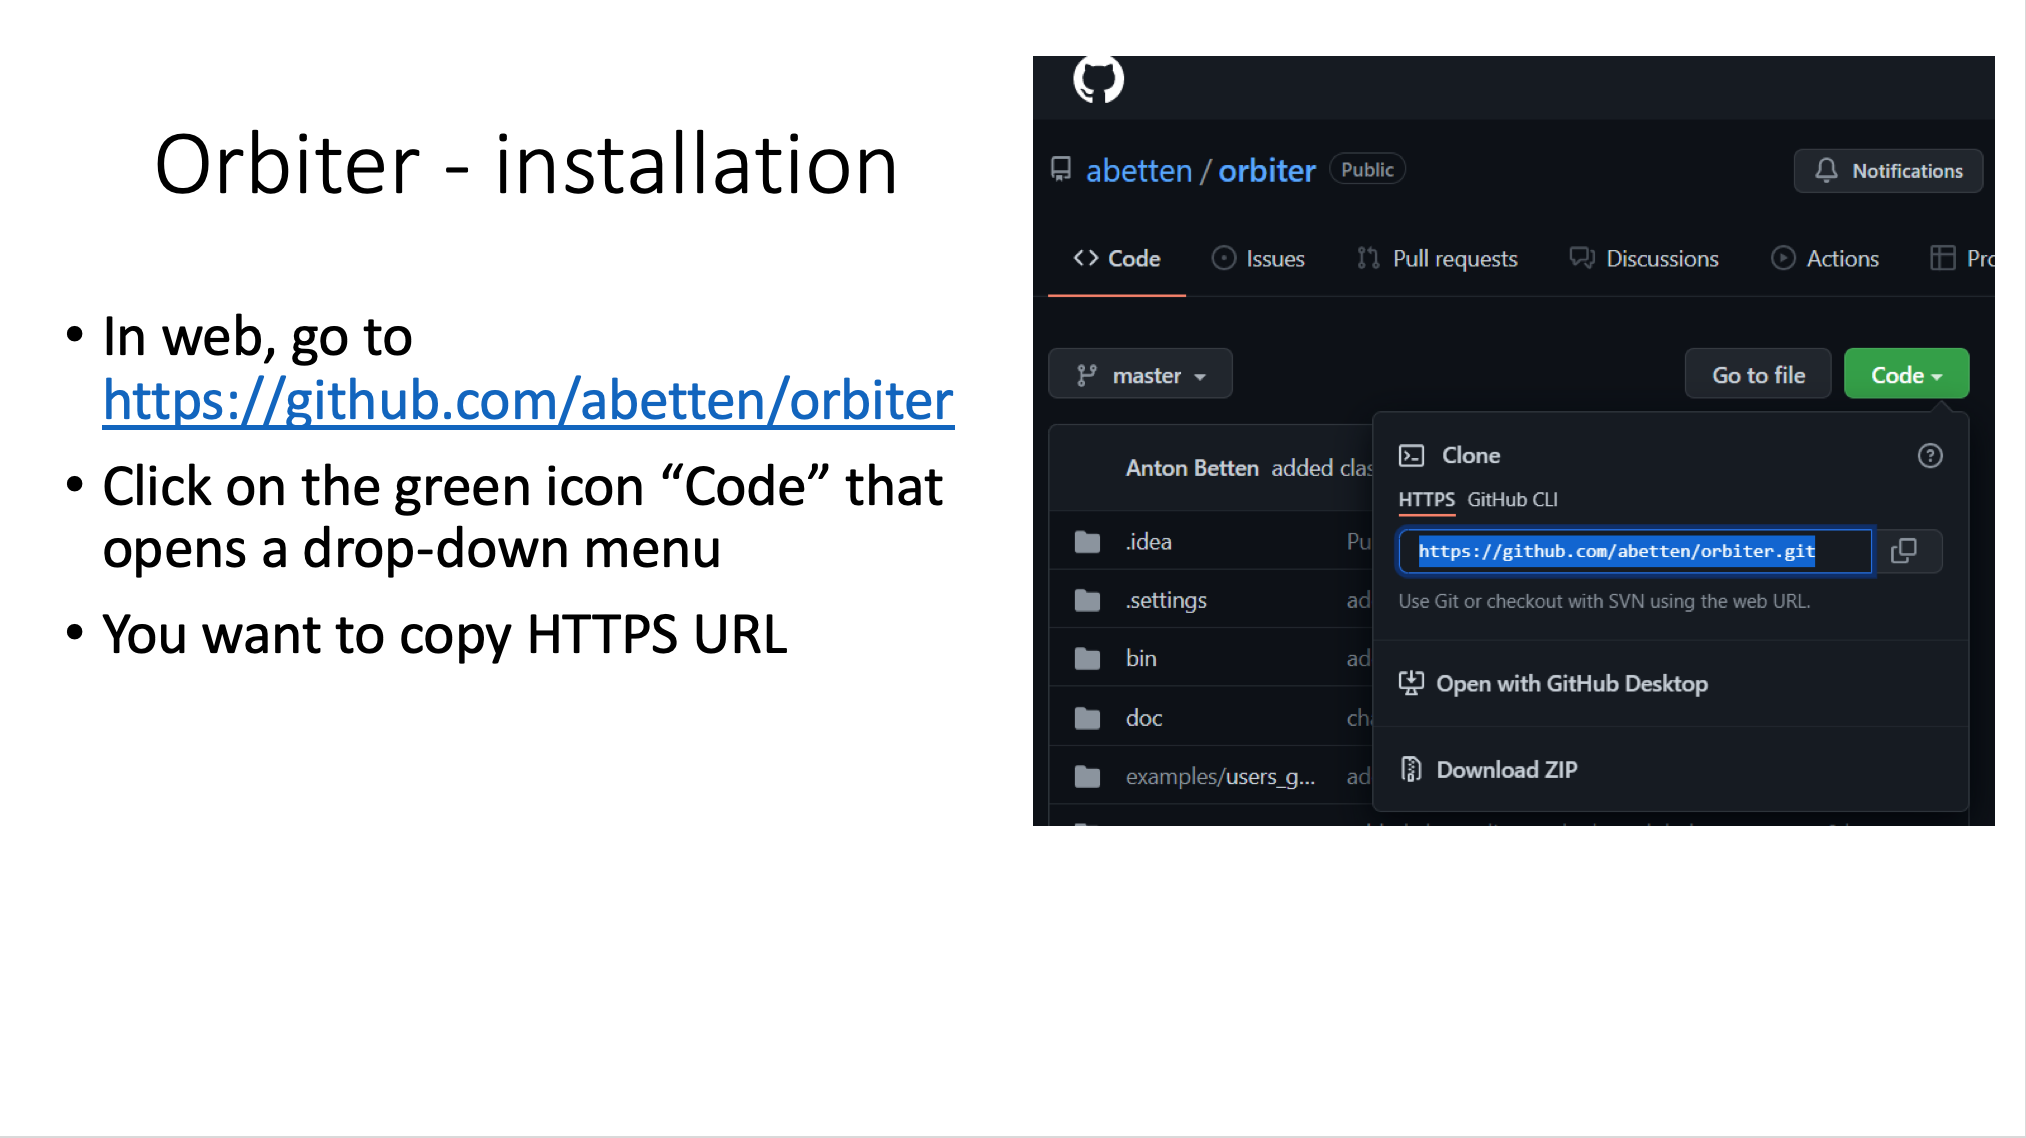
\includegraphics[width=15cm]{GRAPHICS/WIN/win10}
$$

\clearpage

$$
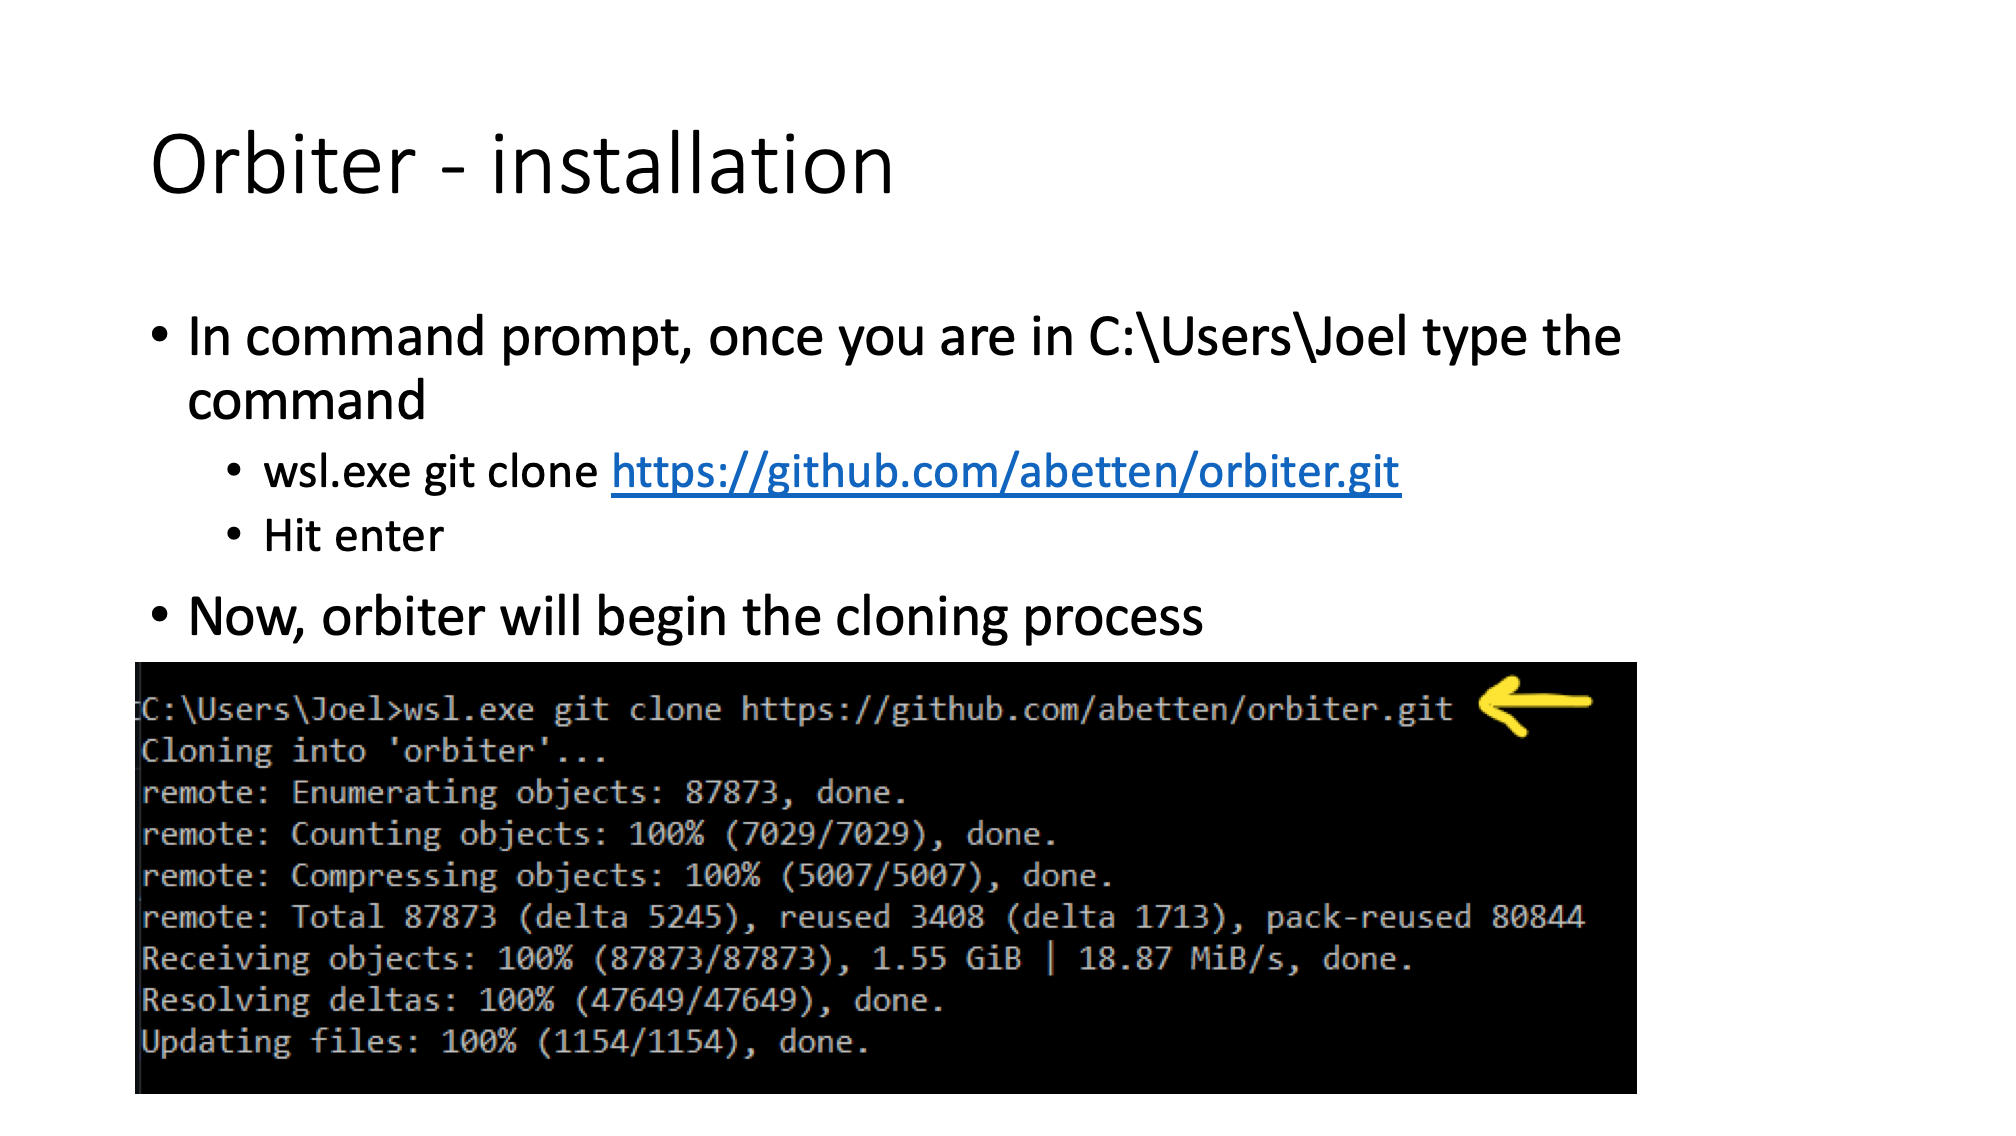
\includegraphics[width=15cm]{GRAPHICS/WIN/win11}
$$
$$
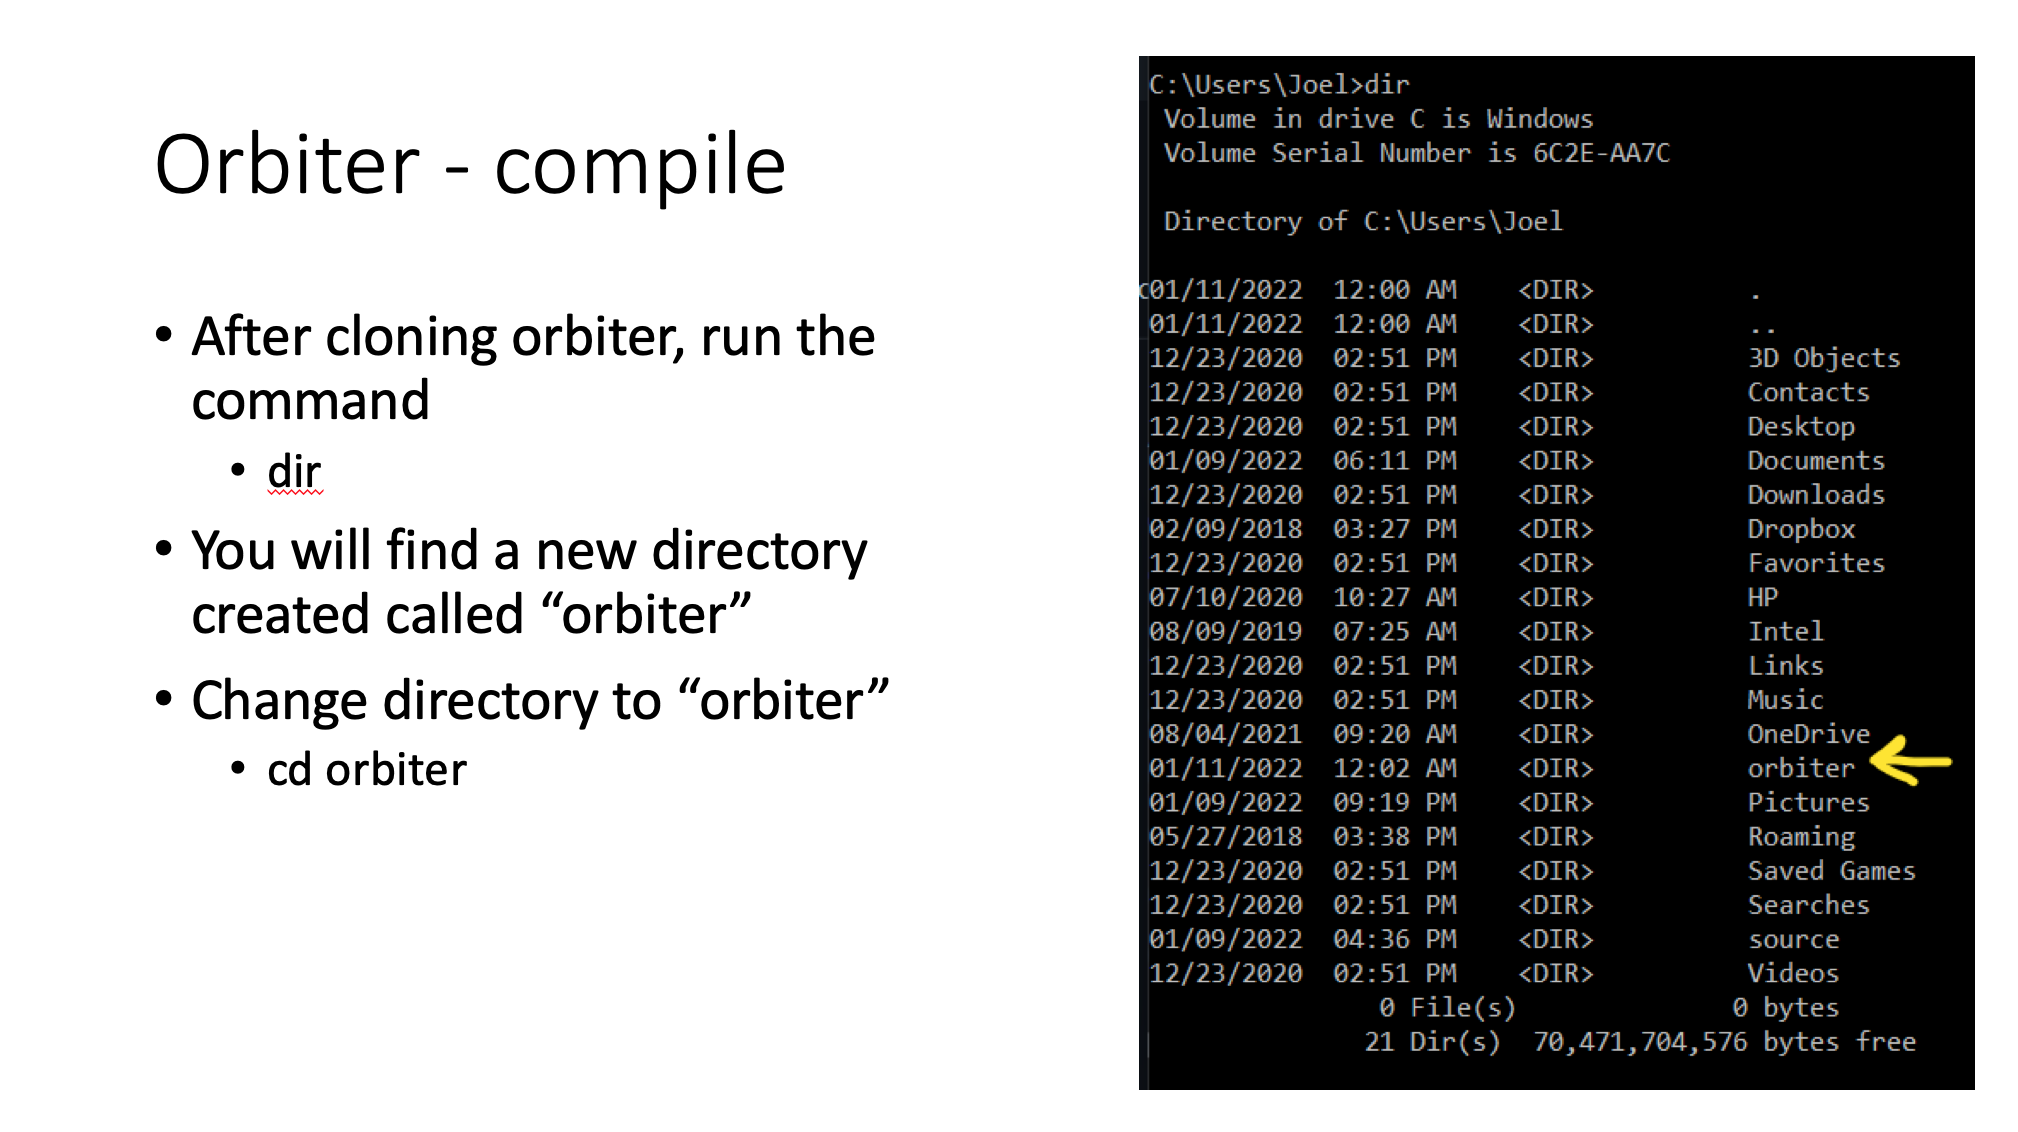
\includegraphics[width=15cm]{GRAPHICS/WIN/win12}
$$

\clearpage

$$
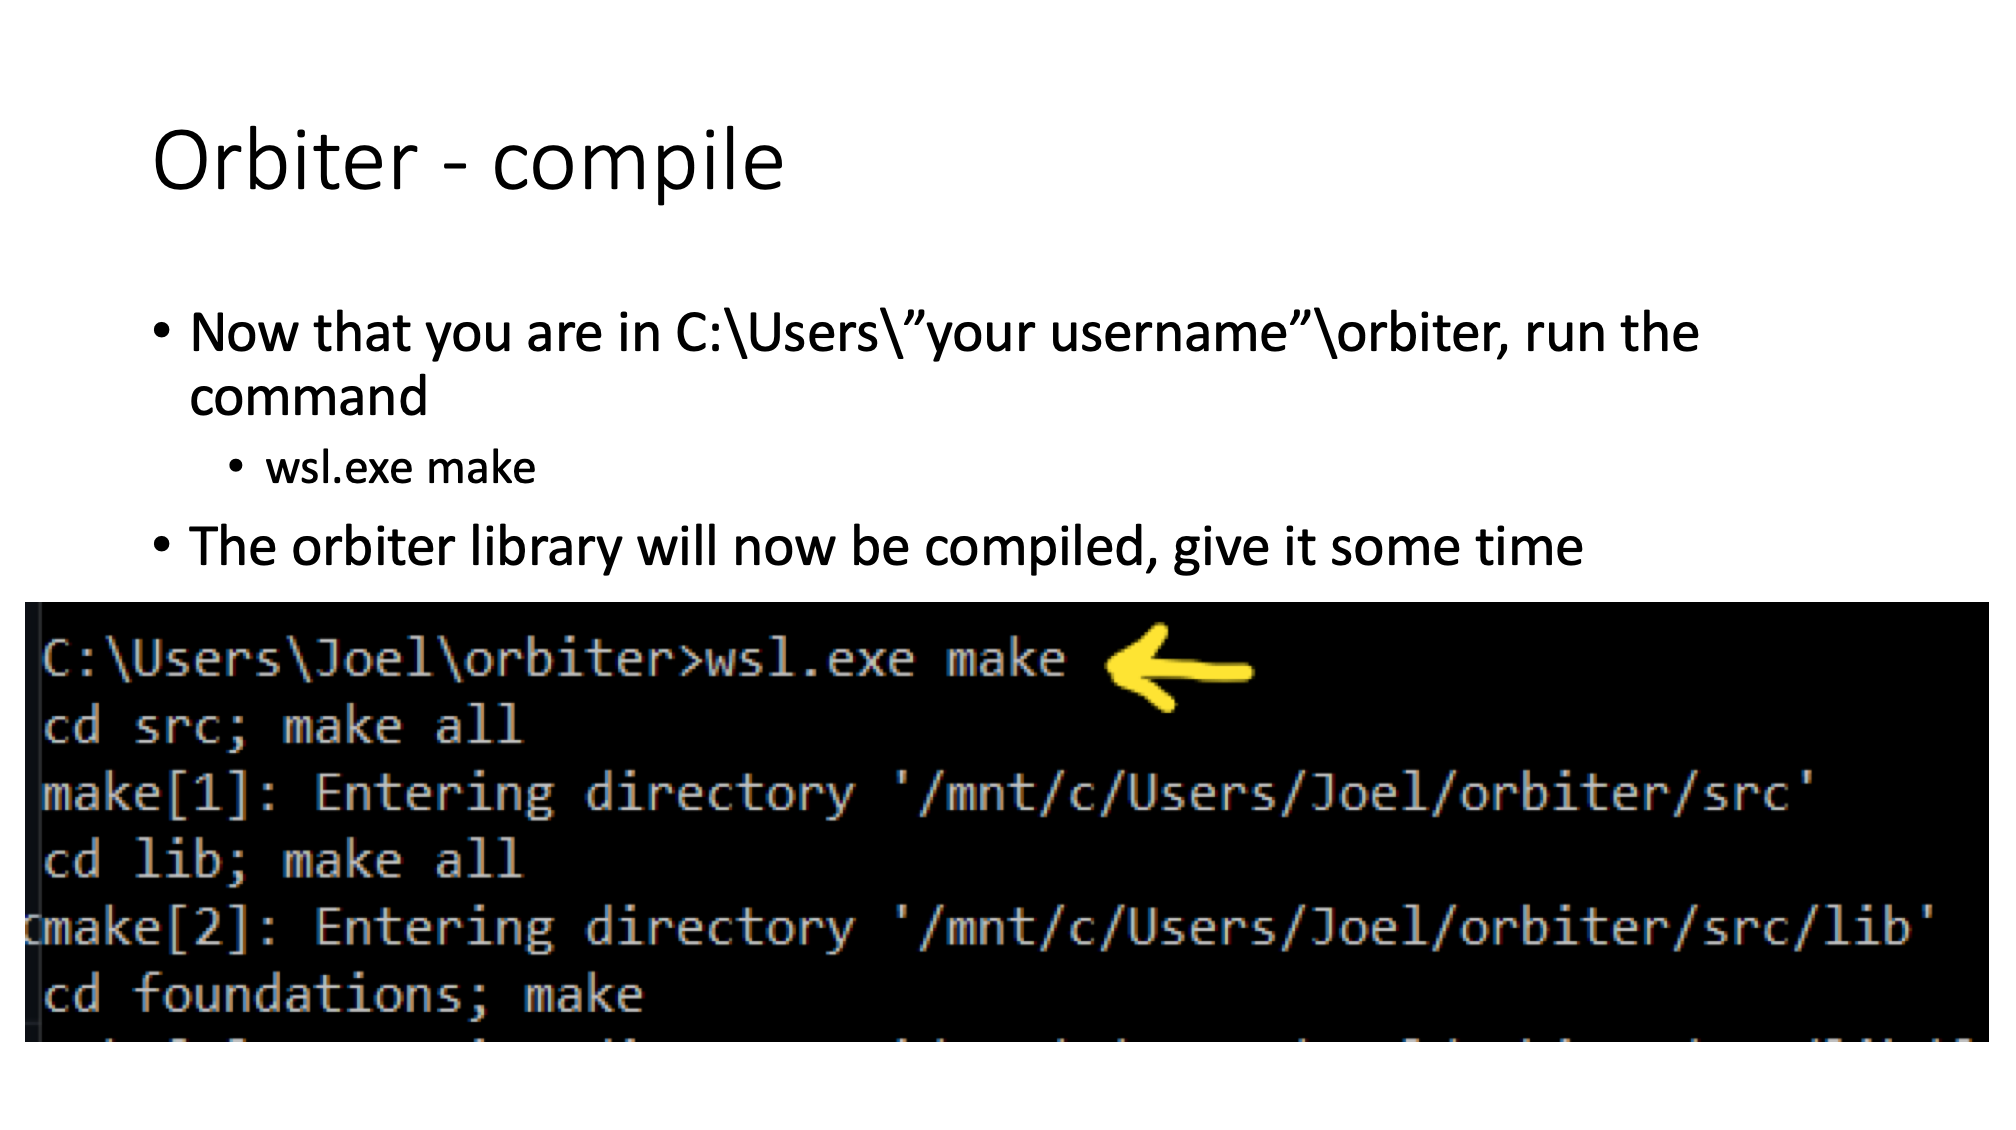
\includegraphics[width=15cm]{GRAPHICS/WIN/win13}
$$
$$
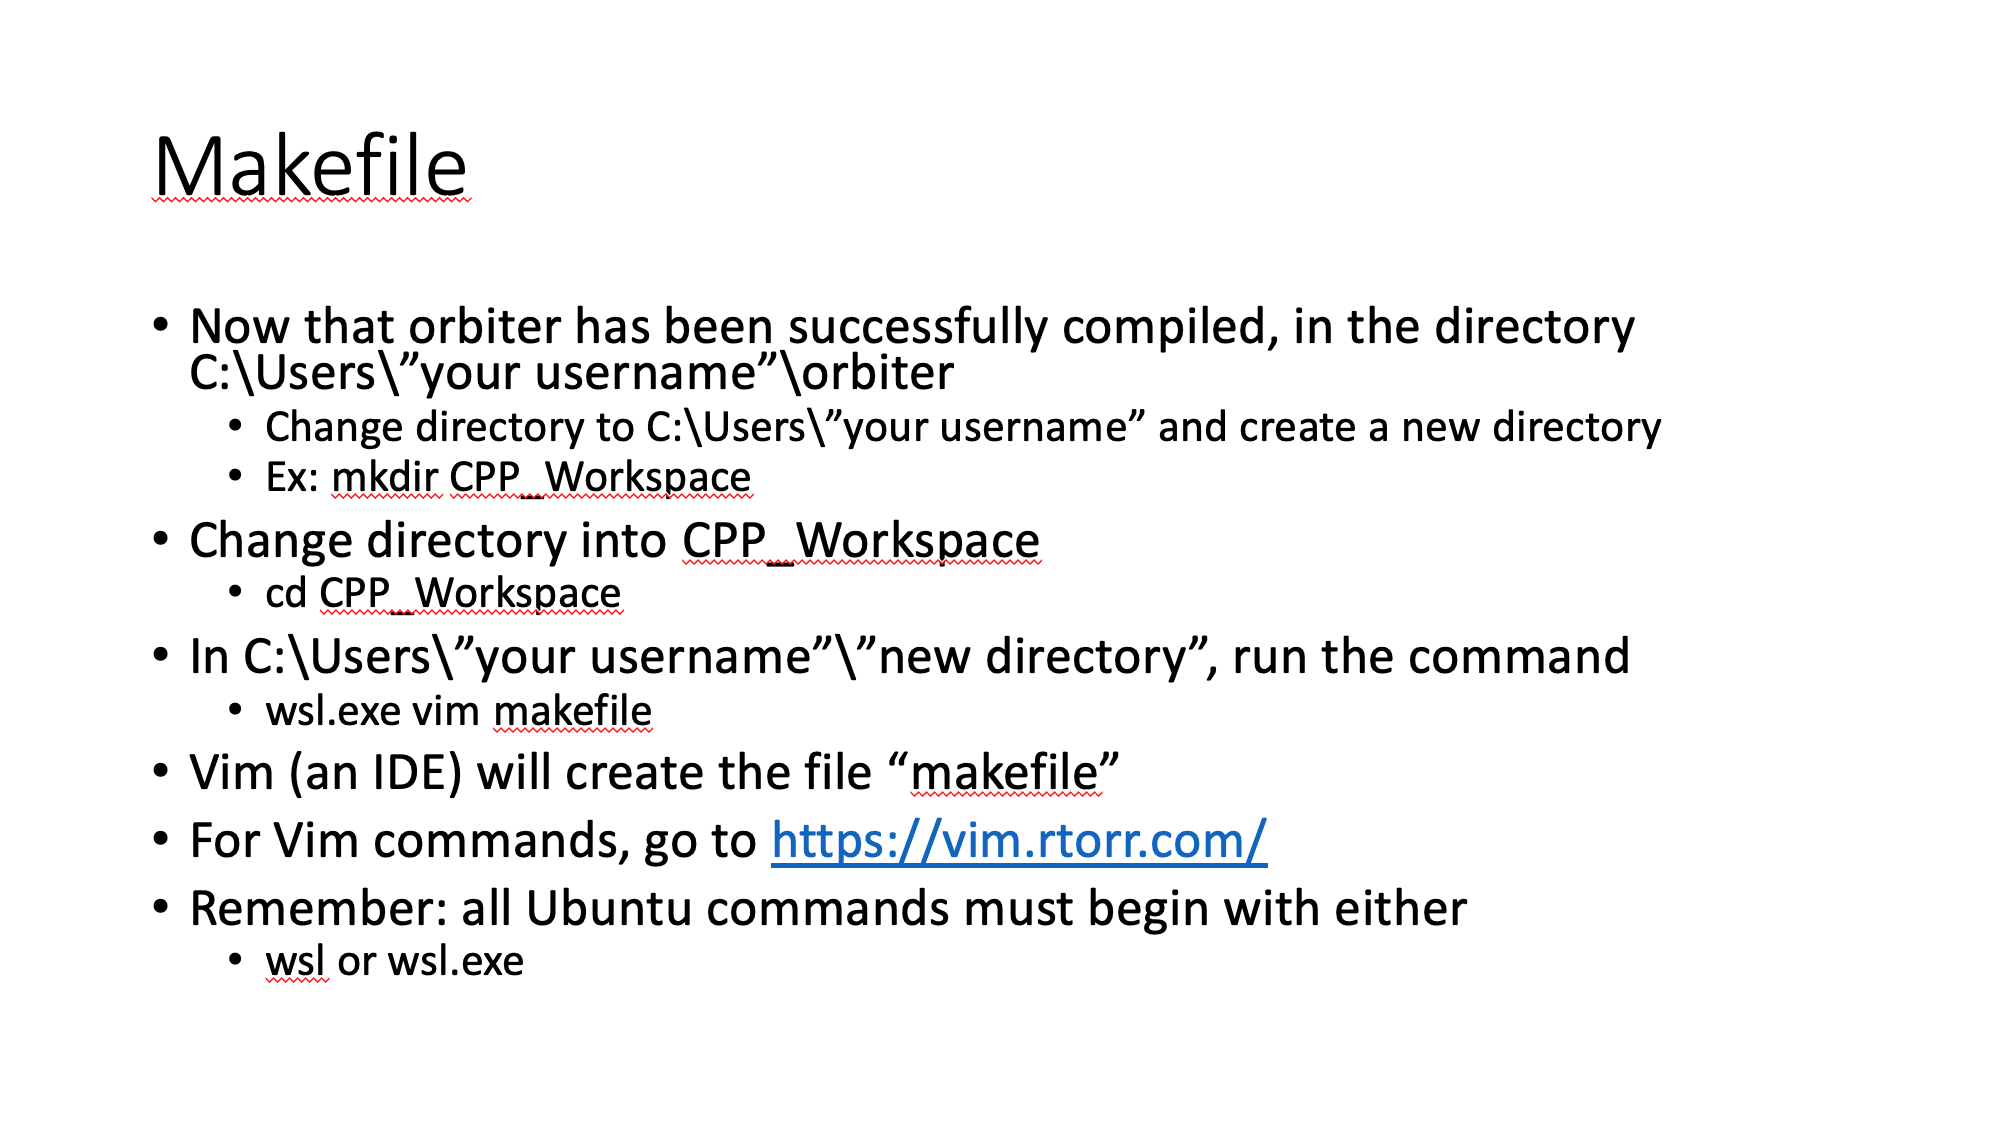
\includegraphics[width=15cm]{GRAPHICS/WIN/win14}
$$

\clearpage

$$
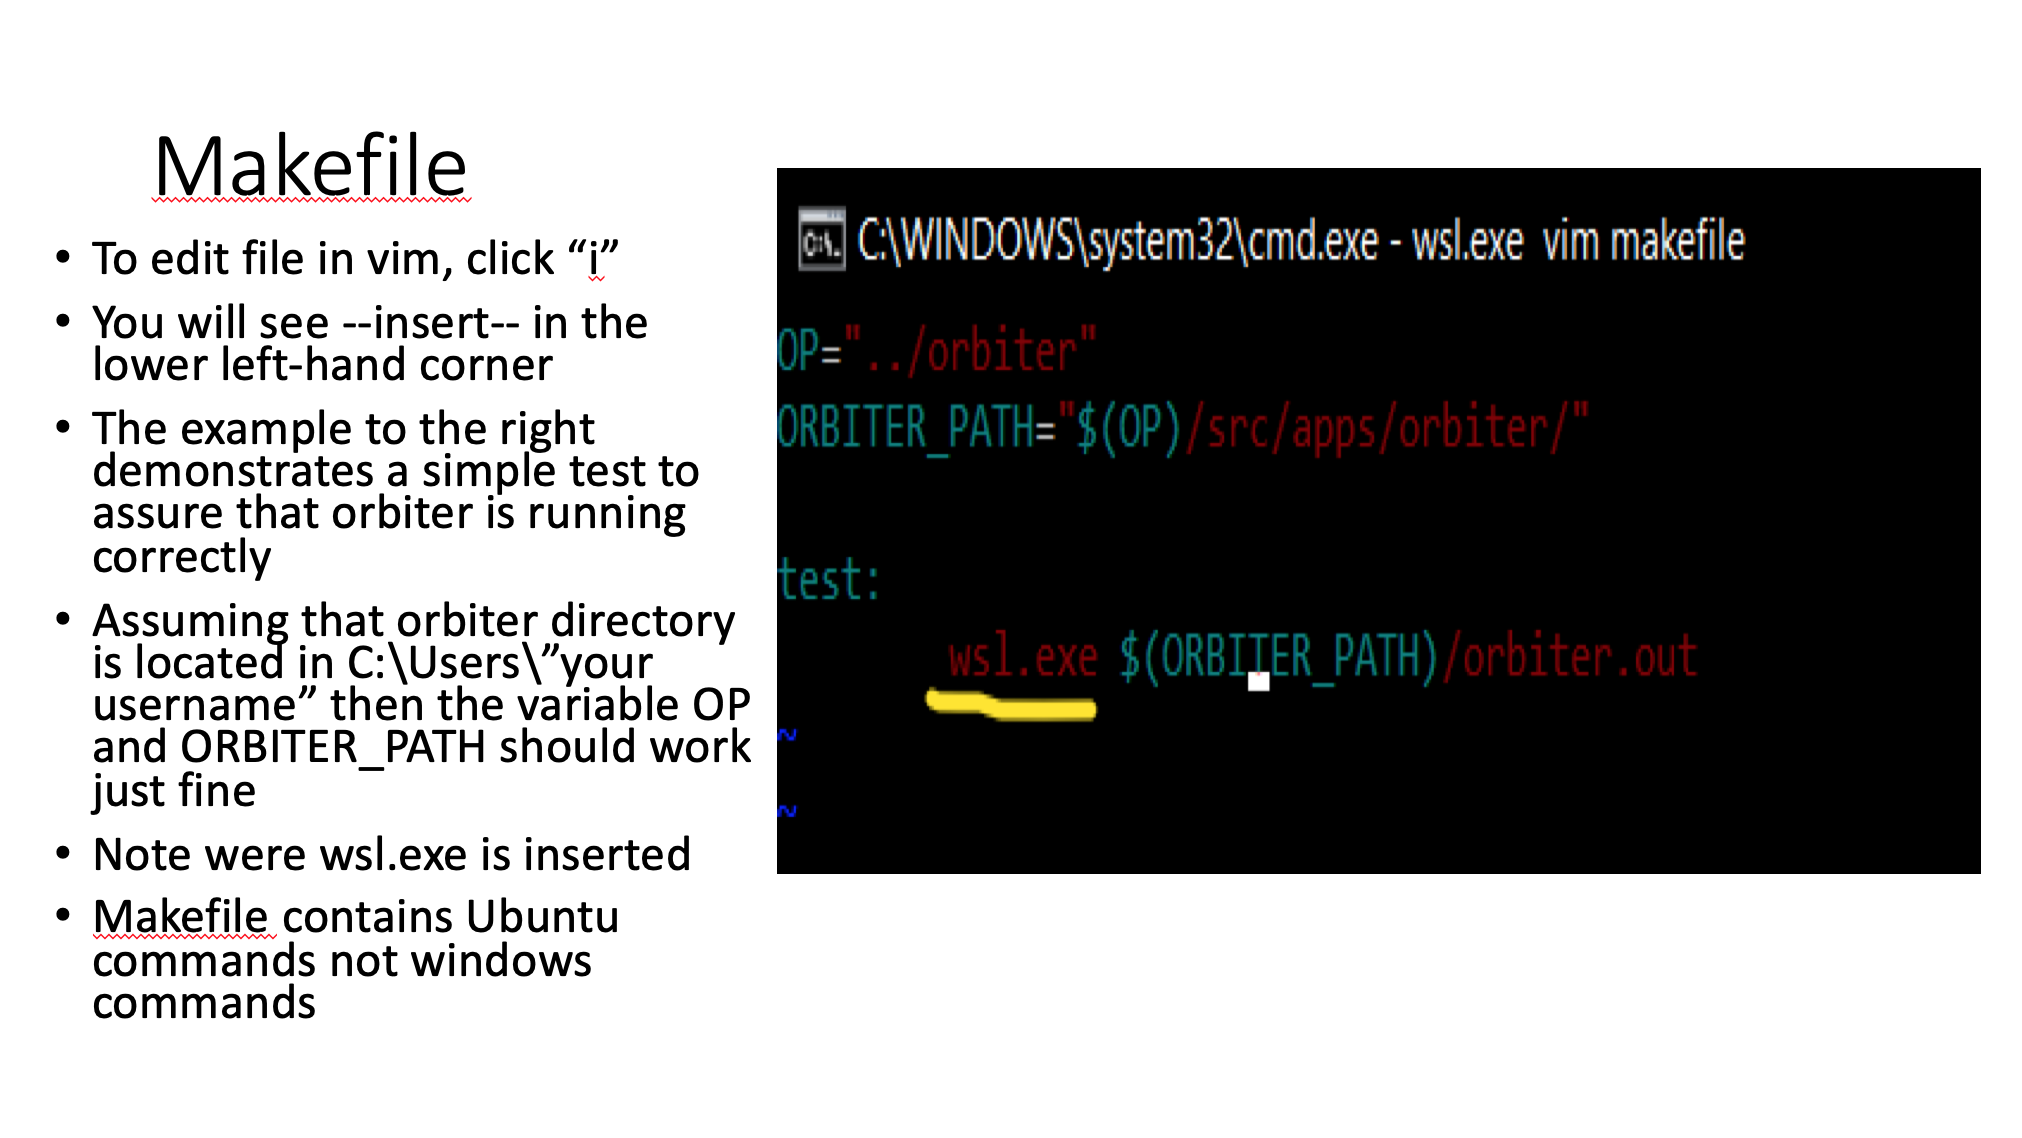
\includegraphics[width=15cm]{GRAPHICS/WIN/win15}
$$
$$
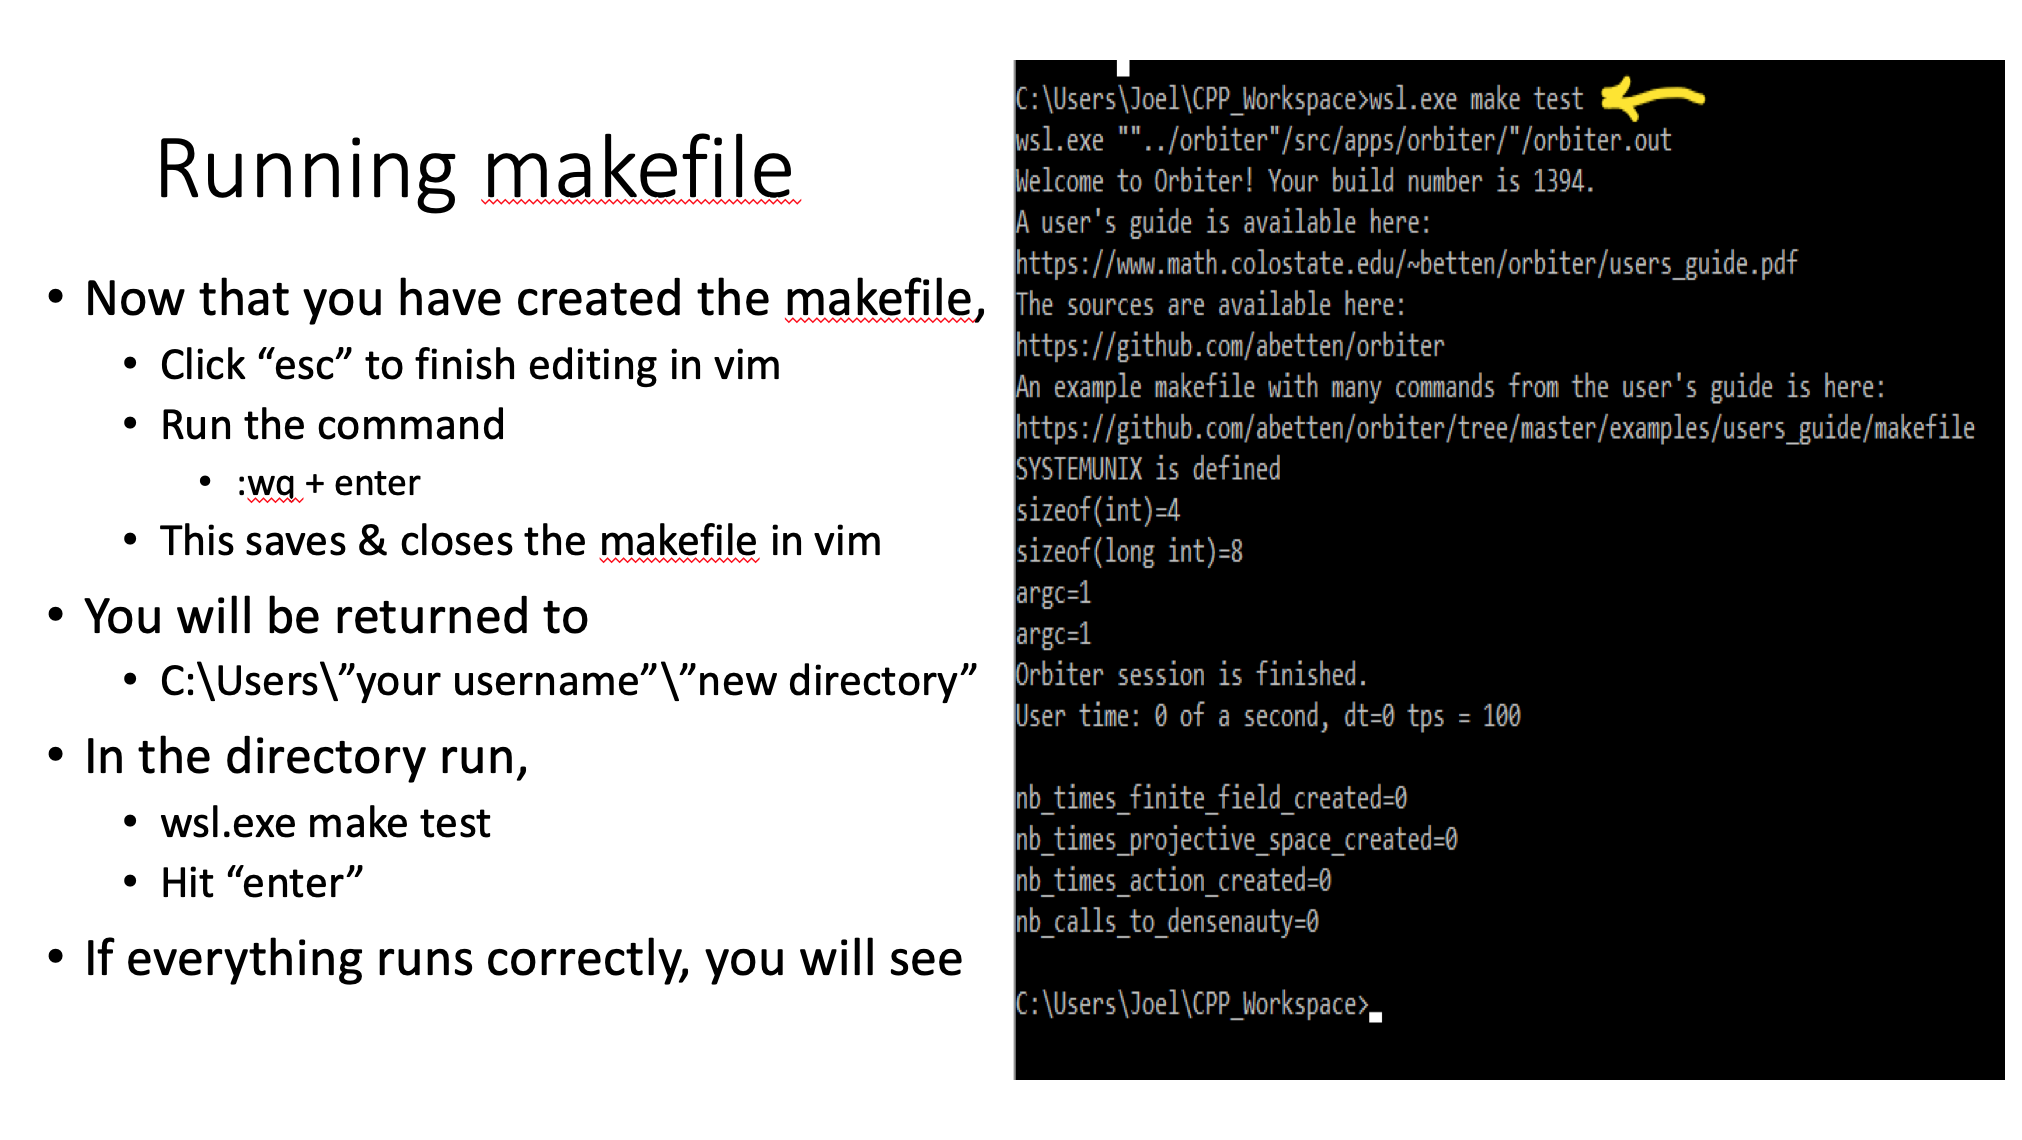
\includegraphics[width=15cm]{GRAPHICS/WIN/win16}
$$

\clearpage

$$
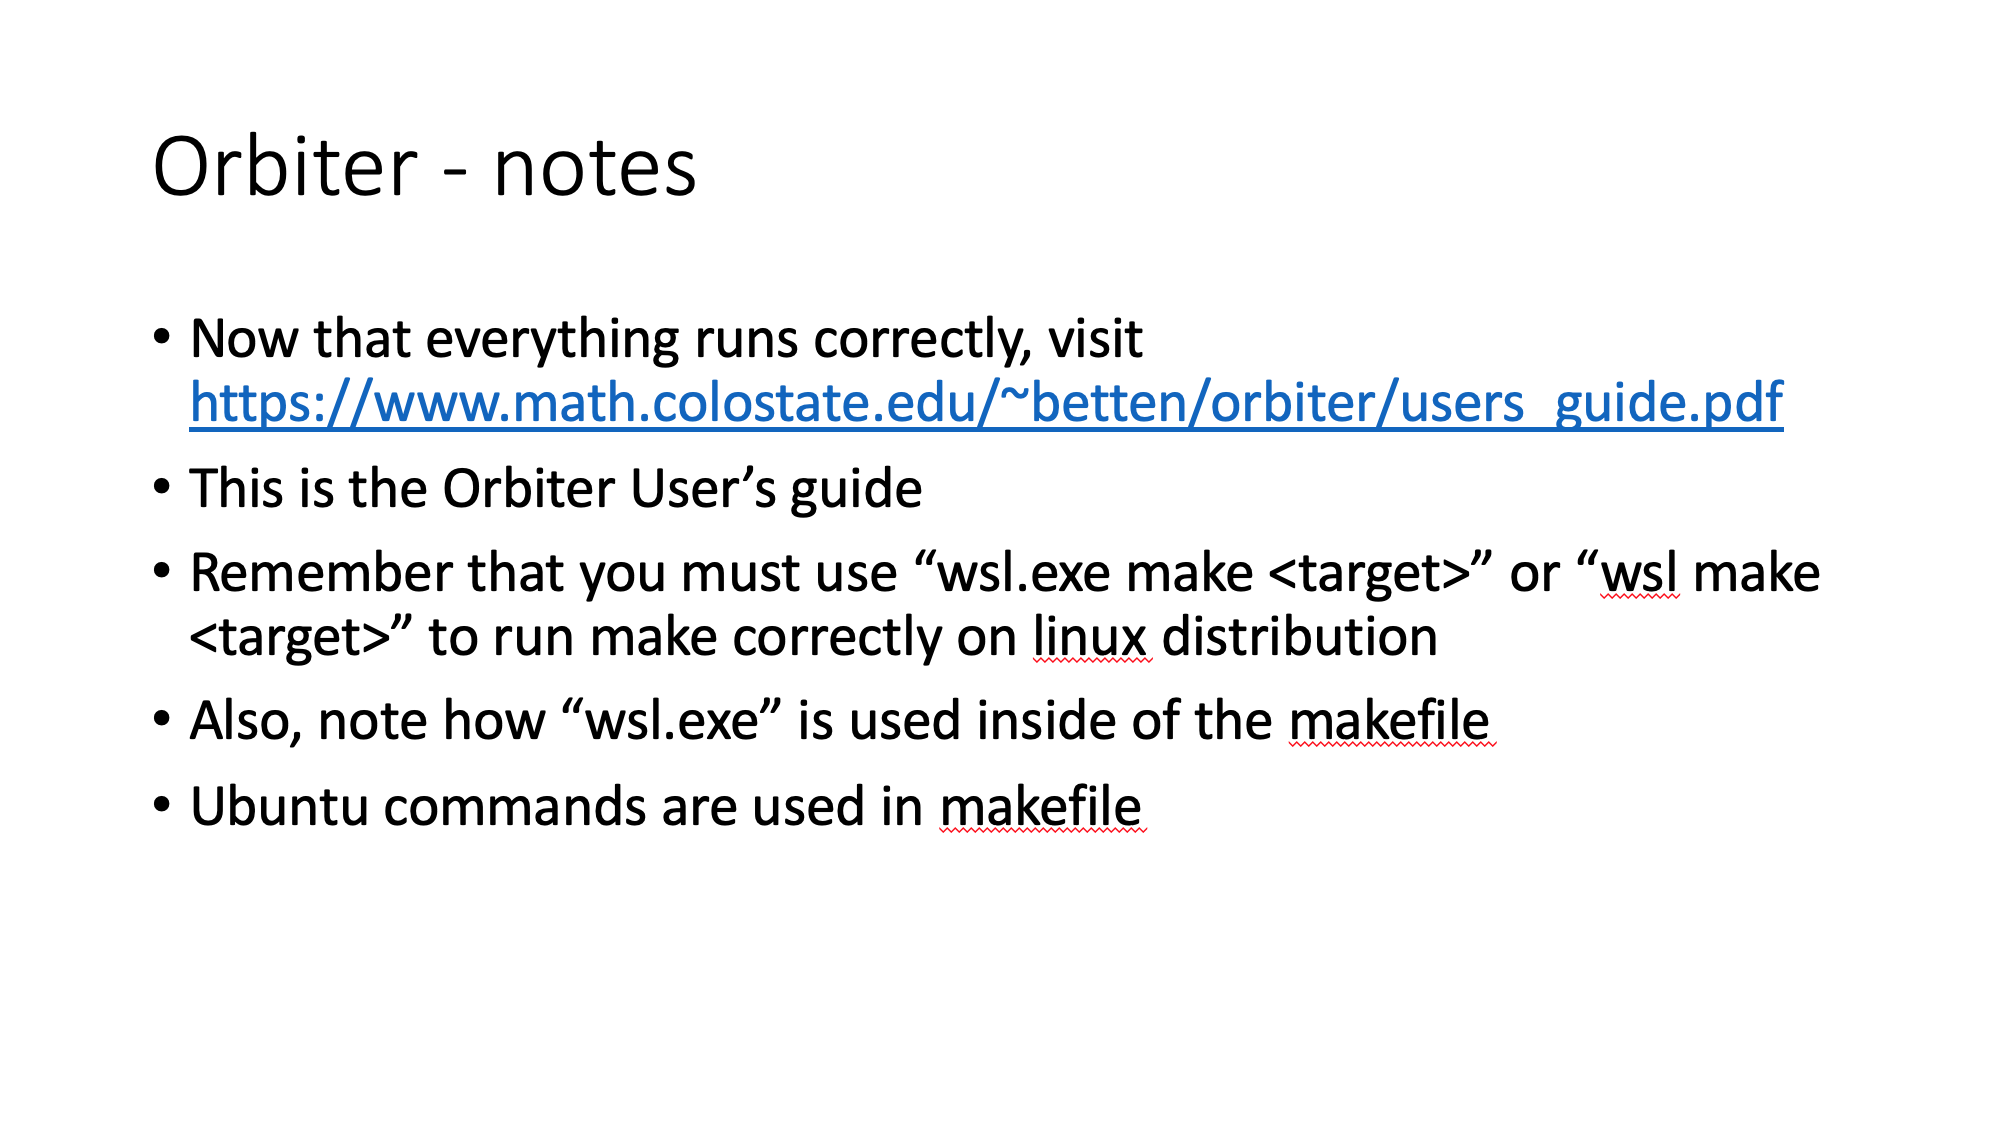
\includegraphics[width=15cm]{GRAPHICS/WIN/win17}
$$
$$
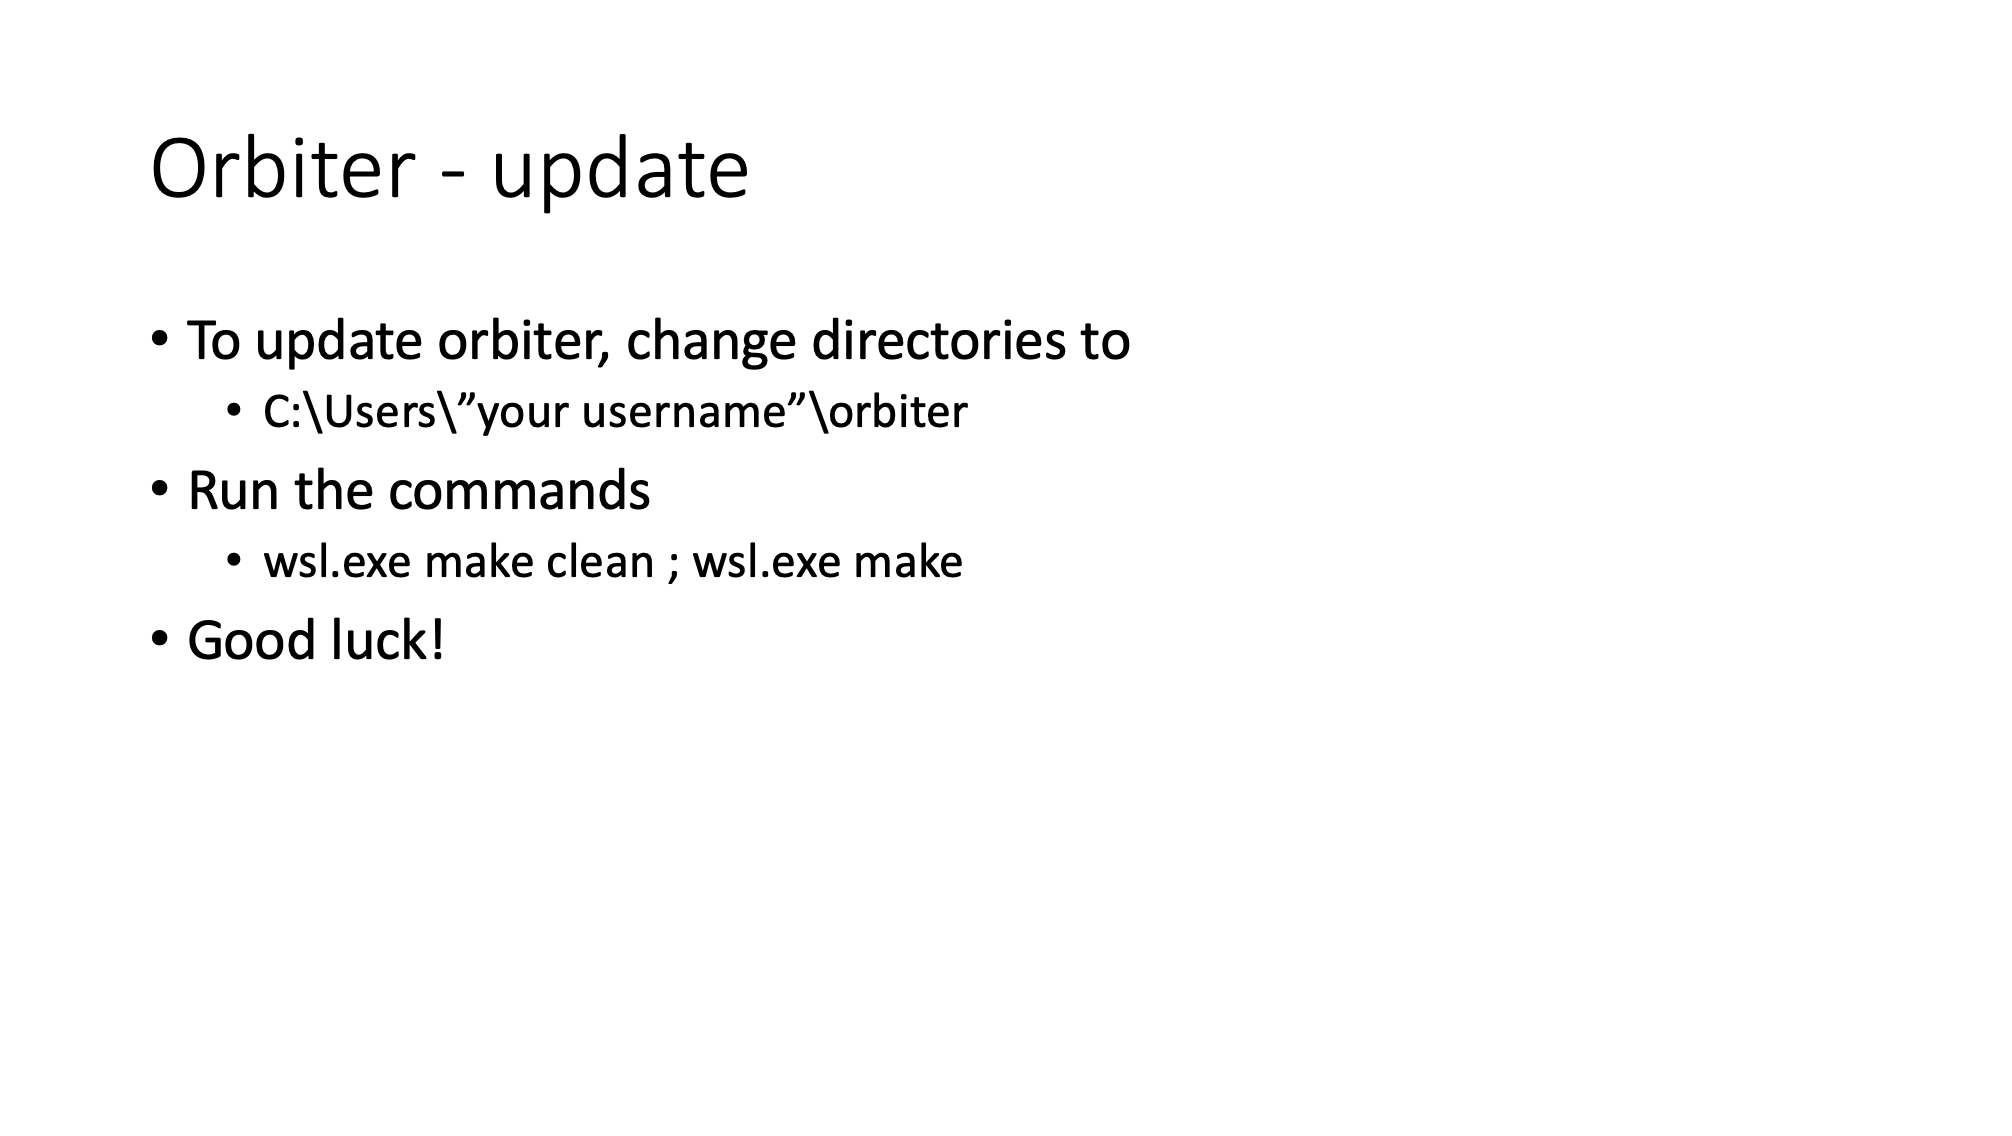
\includegraphics[width=15cm]{GRAPHICS/WIN/win18}
$$

\clearpage



